\documentclass{vutinfth} % Remove option 'final' to obtain debug information.

% Load packages to allow in- and output of non-ASCII characters.
\usepackage{lmodern}        % Use an extension of the original Computer Modern font to minimize the use of bitmapped letters.
\usepackage[T1]{fontenc}    % Determines font encoding of the output. Font packages have to be included before this line.
\usepackage[utf8]{inputenc} % Determines encoding of the input. All input files have to use UTF8 encoding.

% Extended LaTeX functionality is enables by including packages with \usepackage{...}.
\usepackage{amsmath}    % Extended typesetting of mathematical expression.
\usepackage{amssymb}    % Provides a multitude of mathematical symbols.
\usepackage{mathtools}  % Further extensions of mathematical typesetting.
\usepackage{microtype}  % Small-scale typographic enhancements.
\usepackage[inline]{enumitem} % User control over the layout of lists (description, enumerate, description).
\usepackage{multirow}   % Allows table elements to span several rows.
\usepackage{booktabs}   % Improves the typesettings of tables.
\usepackage{subcaption} % Allows the use of subfigures and enables their referencing.
% \usepackage[ruled,linesnumbered,algochapter]{algorithm2e} % Enables the writing of pseudo code.
\usepackage[usenames,dvipsnames,table]{xcolor} % Allows the definition and use of colors. This package has to be included before tikz.
% \usepackage{nag}       % Issues warnings when best practices in writing LaTeX documents are violated.
% \usepackage{todonotes} % Provides tooltip-like todo notes.
\usepackage[colorlinks=false,hidelinks]{hyperref}  % Enables cross linking in the electronic document version. This package has to be included second to last.
% \usepackage[acronym,toc]{glossaries} % Enables the generation of glossaries and lists fo acronyms. This package has to be included last.

\usepackage{breakcites}
\usepackage{amsthm}
\usepackage[normalem]{ulem}
\usepackage{multirow,bigdelim}
\usepackage{enumitem}
\usepackage{siunitx}
\usepackage{musicography}
\usepackage{tcolorbox}

\tcbuselibrary{theorems}
\tcbuselibrary{skins}
\tcbuselibrary{breakable}


%% Colors
%grey
\definecolor{darkCharcoal}{RGB}{30,30,30} % theorem
\definecolor{davys}{RGB}{60,60,60} % proof
\definecolor{sonicSilver}{RGB}{90,90,90} % proposition
\definecolor{gray}{RGB}{120,120,120} % lemma
\definecolor{spanish}{RGB}{150,150,150} % corollary
\definecolor{argent}{RGB}{180,180,180} % example

% blues
\definecolor{azure}{RGB}{0,128,255}
\definecolor{egyptian}{RGB}{16,52,166}
\definecolor{navy}{RGB}{17,30,108}
\definecolor{pastelBlue}{RGB}{0,119,190}

% reds
\definecolor{renate}{RGB}{227,25,113}
\definecolor{burgundy}{RGB}{141,2,31}
\definecolor{salmon}{RGB}{250,128,114}
\definecolor{spanishCrimson}{RGB}{229,26,76}

% yellows
\definecolor{honey}{RGB}{235,150,5}

% green 
\definecolor{pearlAcqua}{RGB}{135,220,192}


%% Environments using tcolorbox
\newtcbtheorem[number within=chapter]
    {thm}
    {Theorem}
    {
        colframe = darkCharcoal,
        colback = white,
        coltitle = white,
        breakable,
        parbox = false,
        separator sign none,
        description delimiters parenthesis,
        enhanced jigsaw,
        sharp corners,
        boxrule = 0.5pt,
        toprule = 1pt,
        bottomrule = 1pt,
        left = 0.2cm,
        right = 0.2cm,
        top = 0.2cm,
        titlerule = 0.5em,
        toptitle = 0.3em,
        bottomtitle = -0.2em,
        %title style={white!25!black},   & <---- remove
        % fonttitle=\bfseries,
        fontupper = \normalsize
    }
    {thm}

\newtcbtheorem
    {prf}
    {Proof}
    {
        colframe = davys,
        colback = white,
        coltitle = white,
        breakable,
        parbox = false,
        enhanced jigsaw,
        sharp corners,
        boxrule = 0.5pt,
        toprule = 1pt,
        bottomrule = 1pt,
        left = 0.2cm,
        right = 0.2cm,
        top = 0.2cm,
        titlerule = 0.5em,
        toptitle = 0.3em,
        bottomtitle = -0.2em,
        %title style={white!25!black},   & <---- remove
        fonttitle=\itshape,
        fontupper = \normalsize
    }
    {prf}

\newtcbtheorem[number within=chapter]
    {prp}
    {Proposition}
    {
        colframe = sonicSilver,
        colback = white,
        coltitle = white,
        breakable,
        parbox = false,
        separator sign none,
        description delimiters parenthesis,
        enhanced jigsaw,
        sharp corners,
        boxrule = 0.5pt,
        toprule = 1pt,
        bottomrule = 1pt,
        left = 0.2cm,
        right = 0.2cm,
        top = 0.2cm,
        titlerule = 0.5em,
        toptitle = 0.3em,
        bottomtitle = -0.2em,
        %title style={white!25!black},   & <---- remove
        % fonttitle=\bfseries,
        fontupper = \normalsize
    }
    {prop}

\newtcbtheorem[number within=chapter]
    {crl}
    {Corollary}
    {
        colframe = gray,
        colback = white,
        coltitle = white,
        breakable,
        parbox = false,
        separator sign none,
        description delimiters parenthesis,
        enhanced jigsaw,
        sharp corners,
        boxrule = 0.5pt,
        toprule = 1pt,
        bottomrule = 1pt,
        left = 0.2cm,
        right = 0.2cm,
        top = 0.2cm,
        titlerule = 0.5em,
        toptitle = 0.3em,
        bottomtitle = -0.2em,
        %title style={white!25!black},   & <---- remove
        % fonttitle=\bfseries,
        fontupper = \normalsize
    }
    {cor}

\newtcbtheorem[number within=chapter]
    {lem}
    {Lemma}
    {
        colframe = spanish,
        colback = white,
        coltitle = white,
        breakable,
        parbox = false,
        separator sign none,
        description delimiters parenthesis,
        enhanced jigsaw,
        sharp corners,
        boxrule = 0.5pt,
        toprule = 1pt,
        bottomrule = 1pt,
        left = 0.2cm,
        right = 0.2cm,
        top = 0.2cm,
        titlerule = 0.5em,
        toptitle = 0.3em,
        bottomtitle = -0.2em,
        %title style={white!25!black},   & <---- remove
        % fonttitle=\bfseries,
        fontupper = \normalsize
    }
    {lem}

\newtcbtheorem[number within=chapter]
    {xmpl}
    {Example}
    {
        colframe = argent,
        colback = white,
        coltitle = white,
        breakable,
        parbox = false,
        % enhanced jigsaw,
        sharp corners,
        boxrule = 0.5pt,
        toprule = 1pt,
        bottomrule = 1pt,
        left = 0.2cm,
        right = 0.2cm,
        top = 0.2cm,
        titlerule = 0.5em,
        toptitle = 0.3em,
        bottomtitle = -0.2em,
        %title style={white!25!black},   & <---- remove
        % fonttitle=\bfseries,
        fontupper = \normalsize
    }
    {ex}

    
%% notation
\newcommand{\poo}[1]{\textcolor{renate}{{#1}-poo}}
\renewcommand{\phi}{\varphi} % variable for formula
\newcommand{\set}[1]{\{{#1}\}} % set
\newcommand{\mods}[1]{[#1]} % models of a formula
\newcommand{\defeq}{\stackrel{\mathclap{\normalfont\mbox{\tiny def}}}{=}} % definition equality






%% propositional logic
\newcommand{\Atoms}{A} % set of propositional atoms
\renewcommand{\L}{\mathcal{L}} % language of propositional logic
\newcommand{\U}{\mathcal{U}} % set of all interpretations
\newcommand{\W}{\mathcal{W}} % set of interpretations
\newcommand{\cn}{{\operatorname{con}}} % consistent
\newcommand{\rf}{{\operatorname{ref}}} % refutable
\newcommand{\comp}{{\operatorname{comp}}} % complete
\newcommand{\dual}[1]{\overline{#1}} % dual of something
\newcommand{\rnm}{\rho} % renaming
\renewcommand{\P}{{\vec{\phi}}} % propositional profile
\newcommand{\append}[2]{{{#1}+{#2}}} % appending a profile to another
\newcommand{\px}{\varepsilon} % proxy for a set of interpretations

%% fragments
\newcommand{\cl}{{\operatorname{Cl}}} % closure
\newcommand{\oocl}[1]{\mathrm{CL}_{#1}} % properties of a closure operator
\newcommand{\oofr}[1]{\mathrm{FR}_{#1}} % properties of a fragment
\newcommand{\horn}{\mathrm{Horn}} % Horn fragment


%% assignments
\newcommand{\as}{\preccurlyeq} % assignment
\newcommand{\totalPre}{\mathrm{total}} % total
\newcommand{\partialPre}{\mathrm{partial}} % partial


%% preferences
\newcommand{\oop}[1]{\mathrm{Pr}_{#1}} % properties of a preference relation
\newcommand{\SPO}{\mathcal{O}} % strict partial orders on a set X
\newcommand{\LIN}{\mathcal{F}} % linear, or full, orders on a set X
\newcommand{\CHN}{\mathcal{C}} % linear, or full, orders on a set X
\newcommand{\PRE}{\mathcal{P}} % preorders on a set X
\newcommand{\TPRE}{\mathcal{T}} % total preorders on a set X
\newcommand{\PP}{{\vec{\le}}} % preference profile


%% distances
\newcommand{\dd}{d} % distance symbol
\newcommand{\ood}[1]{\mathrm{D}_{#1}} % property of a dissimilarity measure
\newcommand{\hamming}{{\operatorname{H}}} % hamming distance
\newcommand{\drastic}{{\operatorname{D}}} % drastic distance





%% aggregation functions
\newcommand{\agg}{{\operatorname{\oplus}}} % aggregation function
\newcommand{\ooa}[1]{\mathsf{Ag}_{{#1}}} % properties of an aggregation function
\newcommand{\ssum}{{\operatorname{sum}}} % sum aggregation function
\newcommand{\leximin}{{\operatorname{leximin}}} % leximin
\newcommand{\leximax}{{\operatorname{leximax}}} % leximax
\newcommand{\lex}{{\operatorname{lex}}} % lexicographic order
\newcommand{\ascending}{{\operatorname{asc}}}
\newcommand{\descending}{{\operatorname{des}}}
\renewcommand{\max}{{\operatorname{max}}}
\renewcommand{\min}{{\operatorname{min}}}







% choice functions 
\newcommand{\cf}{\mathit{c}} % choice function
\newcommand{\ooch}[1]{\mathrm{C}_{#1}} % property for choice function
\newcommand{\scf}{\mathit{sc}} % social choice function
\newcommand{\swf}{\mathit{sw}} % social welfare function
\newcommand{\VV}{\vec{V}} % approval profile
\newcommand{\abc}{{\operatorname{abc}}} % abc voting rule



%% varieties of belief change
\newcommand{\bc}{\musFlat{}} % general elief change operator
\newcommand{\re}{\circ} % revision operator
\newcommand{\en}{\triangleright} % enforcement operator
\newcommand{\up}{\diamond} % update operator
\newcommand{\me}{\Delta} % merging operator

\newcommand{\ppr}[1]{\mathrm{R}_{#1}} % postulate for revision
\newcommand{\ppu}[1]{\mathrm{U}_{#1}} % postulate for update
\newcommand{\ppe}[1]{\mathrm{E}_{#1}} % postulate for enforcement
\newcommand{\ppm}[1]{\mathrm{M}_{#1}} % postulate for merging
\newcommand{\ppp}[1]{\mathrm{P}_{#1}} % postulate for preference change

\newcommand{\oor}[1]{\mathrm{r}_{#1}} % properties of the assignment for revision
\newcommand{\oou}[1]{\mathrm{u}_{#1}} % properties of the assignment for update
\newcommand{\ooe}[1]{\mathrm{e}_{#1}} % properties of the assignment for enforcement
\newcommand{\oom}[1]{\mathrm{m}_{#1}} % properties of the assignment for merging

\newcommand{\exh}{{\operatorname{exh}}} % exhaustive revealed assignment
\newcommand{\exc}{{\operatorname{exc}}} % exclusive revealed assignment 

\newcommand{\wb}{\mathrm{wb}} % worst-to-best levels
\newcommand{\bw}{\mathrm{bw}} % best-to-worst levels
\newcommand{\rem}{\mathtt{rem}} % remove operator

\newcommand{\symdiff}{\mathtt{symdiff}} % symmetric difference

\newcommand{\add}{{\operatorname{add}}} % add operator





%% revision with varying attitudes
\newcommand{\ctr}{\mathrm{cen}} % centrality
\newcommand{\dis}{\mathrm{dis}} % displacement
\newcommand{\agr}{\mathrm{agr}} % agreeability index
\newcommand{\dagr}{\mathrm{dagr}} % disagreeability index
\newcommand{\summing}{\mathrm{sum}} % sum
\newcommand{\forgetful}{\mathrm{F}}

\newcommand{\bld}{{\mathrm{bold}}}
\newcommand{\conservative}{{\mathrm{csrv}}}

\newcommand{\IAHB}{\mathsf{IAHB}} % indifference to already held beliefs
\newcommand{\STAB}{\mathsf{STAB}} % stability
\newcommand{\NEUT}{\mathsf{NEUT}} % neutrality


%% social merging
\newcommand{\perm}{\sigma} % permutations
\newcommand{\bndl}{\rightsquigarrow} % bundling operator

\newcommand{\supp}{{\operatorname{supp}}} % support of one interpretation over another

\newcommand{\MAJ}{\mathsf{MAJ}}
\newcommand{\ARB}{\mathsf{ARB}}

\newcommand{\ANON}{\mathsf{ANON}}
\newcommand{\BNDL}{\mathsf{BNDL}}
\newcommand{\NOND}{\mathsf{NOND}} % non-dictatorship
\newcommand{\WPRT}{\mathsf{wPAR}} % weak Pareto
\newcommand{\SPRT}{\mathsf{sPAR}} % strong Pareto
\newcommand{\CSOV}{\mathsf{CSOV}} % citizen sovereignty
\newcommand{\COND}{\mathsf{COND}} % condorcet
\newcommand{\MAJR}{\mathsf{MAJR}} % majority
\newcommand{\MONO}{\mathsf{MONO}}
\newcommand{\PART}{\mathsf{PART}}
\newcommand{\RSYM}{\mathsf{RSYM}}
\newcommand{\RSVB}{\mathsf{RSVB}}
\newcommand{\ICLN}{\mathsf{ICLN}}
\newcommand{\CONS}{\mathsf{CONS}}
\newcommand{\HOMG}{\mathsf{HOMG}}
\newcommand{\INDC}{\mathsf{INDC}}
\newcommand{\SLFA}{\mathsf{SLFA}}
 




%% manipulability
\newcommand{\w}{w}
\newcommand{\hammingdist}{d_H}
\newcommand{\drasticdist}{d_D}
\newcommand{\aggsum}{\Sigma}
\newcommand{\aggmax}{\mathtt{max}}
\newcommand{\agggmax}{\mathtt{gmax}}
\newcommand{\aggop}[2]{\Delta^{#1}_{#2}}
\newcommand{\Aggop}[1]{\Delta^{#1}}
\newcommand{\Agg}[3]{\Aggop{{#1}}_{{#2}}({#3})}
\newcommand{\df}{d,\,f}
\newcommand{\hs}{\hammingdist,\,\aggsum}
\newcommand{\hg}{\hammingdist,\,\agggmax}
\newcommand{\hm}{\hammingdist,\,\aggmax}
\newcommand{\ds}{\drasticdist,\,\aggsum}
\newcommand{\dg}{\drasticdist,\,\agggmax}
\newcommand{\dm}{\drasticdist,\,\aggmax}

\newcommand{\Amp}{\Agg{}{\mu}{P}}
\newcommand{\Adfmp}{\Agg{\df}{\mu}{P}}
\newcommand{\Ahsmp}{\Agg{\hs}{\mu}{P}}
\newcommand{\Ahmmp}{\Agg{\hm}{\mu}{P}}
\newcommand{\Ahgmp}{\Agg{\hg}{\mu}{P}}
\newcommand{\Adsmp}{\Agg{\ds}{\mu}{P}}
\newcommand{\Adgmp}{\Agg{\dg}{\mu}{P}}

\newcommand{\Am}[1]{\Agg{}{\mu}{{#1}}}
\newcommand{\Adfm}[1]{\Agg{\df}{\mu}{{#1}}}
\newcommand{\Ahsm}[1]{\Agg{\hs}{\mu}{{#1}}}
\newcommand{\Ahmm}[1]{\Agg{\hm}{\mu}{{#1}}}
\newcommand{\Ahgm}[1]{\Agg{\hg}{\mu}{{#1}}}
\newcommand{\Adsm}[1]{\Agg{\ds}{\mu}{{#1}}}
\newcommand{\Adgm}[1]{\Agg{\dg}{\mu}{{#1}}}

\newcommand{\acc}{{\operatorname{acc}}}
\newcommand{\cred}{{\operatorname{cred}}}
\newcommand{\skept}{{\operatorname{skept}}}
\newcommand{\no}{\mathtt{No}}
\newcommand{\credsupp}{{\cred\operatorname{supp}}}
\newcommand{\skeptsupp}{{\skept\operatorname{supp}}}

\newcommand{\icred}{i_{\cred}}
\newcommand{\iskept}{i_{\skept}}
\newcommand{\ino}{i_{\no}}

\newcommand{\idw}{i_{\mathtt{dw}}}
\newcommand{\ids}{i_{\mathtt{ds}}}
\newcommand{\ip}{i_{\mathtt{p}}}

\newcommand{\truth}[1]{{#1}^{\mathtt{t}}}
\newcommand{\manip}[1]{{#1}^{\mathtt{f}}}







% proportionality
\newcommand{\sat}{s} % satisfaction

\newcommand{\amax}{\mathrm{max}}
\newcommand{\amin}{\mathrm{min}}
\newcommand{\mer}[2]{\Delta^{#1}_{#2}}

\newcommand{\IC}[1]{\mathsf{IC}_{#1}} % IC postulates
\newcommand{\MI}[1]{\mathsf{D}_{#1}} % properties of a maximizing assignment
\newcommand{\MA}[1]{\mathsf{O}_{#1}} % properties of a minimizing assignment
\newcommand{\SM}[1]{\mathsf{S}_{#1}} % properties of a satisfaction measure

\newcommand{\av}{\mathrm{AV}}
\newcommand{\sav}{\mathrm{SAV}}
\newcommand{\pav}{\mathrm{PAV}}
\newcommand{\bpav}{\mathrm{bPAV}}
\newcommand{\hd}{{h(s_d)}}
\newcommand{\hhamming}{\mathrm{hH}}
\newcommand{\hdrastic}{\mathrm{hD}}
\newcommand{\sdrastic}{\mathrm{sD}}
%\newcommand{\csat}{\mathit{csat}}
%\newcommand{\bsat}{\mathit{bsat}}
\newcommand{\CPROP}{\mathsf{CPROP}} % weak classical proportionality
\newcommand{\BPROP}{\mathsf{BPROP}} % weak binary proportionality





%Horn update
\newcommand{\HPH}{{\mathrm{HPH}}}
\newcommand{\HHH}{{\mathrm{HHH}}}

\newcommand{\intrs}{\operatorname{ints}} % intersect function

\newcommand{\PCMPL}{\mathrm{pC}} % pair compliance
\newcommand{\TCMPL}{\mathrm{tC}} % triple compliance
\newcommand{\dTCMPL}{\mathrm{dTCMPL}} % extended triple compliance
\newcommand{\HC}{\mathrm{HC}} % Horn compliance

\newcommand{\SCON}{{\mathrm{SC}}}
\newcommand{\HSCON}{{\mathrm{HSC}}}
\newcommand{\SCXH}{{\mathrm{SC}{-}\mathrm{exh}}} % Suzumura consistency for exhaustive 
\newcommand{\SCXC}{{\mathrm{SC}{-}\mathrm{exc}}} % Suzumura consistency for exclusive

\newcommand{\A}{\mathsf{A}}
\newcommand{\Astar}{\mathsf{A}\star}
\newcommand{\prop}{\mathcal{L}}
\newcommand{\krom}{\mathsf{2CNF}}
\newcommand{\lits}{\mathsf{1CNF}}
\newcommand{\Lhorn}{\L_{\mathsf{Horn}}}
\newcommand{\Lkrom}{\L_{\mathsf{2CNF}}}
\newcommand{\Llits}{\L_{\mathsf{1CNF}}}
\newcommand{\closureOp}{\mathsf{Cl}}
\newcommand{\maj}{\mathrm{maj}}
\newcommand{\id}{\mathrm{id}}

\newcommand{\sd}{\bigtriangleup} %sd for symmetric difference
\newcommand{\mins}[1]{\min_\subseteq {#1}}
\newcommand{\mint}[1]{\min_{\le_w^T}  {#1}}
\newcommand{\minb}[1]{\min_{\le_w^B}  {#1}}
\newcommand{\minc}[1]{\min_{\textnormal{\tiny card}} {#1}}

\newcommand{\ffrm}[2]{\px^{{#1}}_{{#2}}} % formula representing #2 in fragment #1
\newcommand{\frm}[1]{\px_{{#1}}} % formula representing #1
\newcommand{\srev}{\lhd} % revealed ranking strict
\newcommand{\rev}{\unlhd} % revealed ranking

\newcommand{\rop}{\circ} %change operator
\newcommand{\uop}{\diamond} %update operator
\newcommand{\uopB}{\diamond^B} % basic update operator
\newcommand{\uopT}{\diamond^T} %trivial update operator
\newcommand{\upB}[2]{{#1}\uopB {#2}} % basic update #1 by #2
\newcommand{\upT}[2]{{#1}\uopT {#2}} % trivial update #1 by #2
\newcommand{\upp}[3]{{#1}\uop^{#3} {#2}} % update #1 by #2 of type #3
\newcommand{\upF}{\uop^F}
\newcommand{\upW}{\uop^W}
\newcommand{\fo}[2]{#1\upF #2} %Forbus's operator
\newcommand{\wi}[2]{#1\upW #2} %Winslett's operator

%% postulates and properties
\newcommand{\faith}[1]{$\mathsf{f}_{#1}$} % faithful assignment properties


%% preference change
\newcommand{\p}{\pi} % preference order being revised
\renewcommand{\d}{\delta} % set of direct comparisons
\renewcommand{\o}{o} % preference order that is revising
\newcommand{\pP}{\mathsf{P}} % postulate for preference revision
\newcommand{\cyc}[2]{\kappa_{#1}^{#2}} % direct comparisons of #1 involved in a cycle induced by #2
\newcommand{\cycfree}[2]{\alpha_{#1}^{#2}} % cycle free part of #1 \cup #2
\newcommand{\upper}[1]{\lfloor{#1}\rfloor} % 
\newcommand{\upperd}[1]{\lfloor{#1}\rfloor^\mathsf{D}} % 

\newcommand{\addc}{{\operatorname{addc}}} % add comparison operator


\newcommand{\dir}{\delta} % direct comparisons
\newcommand{\nb}{\mathrm{nb}} % next-best elements
\newcommand{\lvl}{\mathit{lvl}} % best-to-worst levels
\newcommand{\tightplus}[2]{{#1}{+}{#2}} % writes #1 {+} #2
\newcommand{\drc}[1]{({#1},\tightplus{#1}{1})} % direct comparison starting with #1
\newcommand{\asignment}{a} % assignment
% Define convenience functions to use the author name and the thesis title in the PDF document properties.
\newcommand{\authorname}{Adrian Haret} % The author name without titles.
\newcommand{\thesistitle}{Choosing What to Believe} % The title of the thesis. The English version should be used, if it exists.

% Set PDF document properties
\hypersetup{
    pdfpagelayout   = TwoPageRight,           % How the document is shown in PDF viewers (optional).
    linkbordercolor = {Melon},                % The color of the borders of boxes around crosslinks (optional).
    pdfauthor       = {\authorname},          % The author's name in the document properties (optional).
    pdftitle        = {\thesistitle},         % The document's title in the document properties (optional).
    pdfsubject      = {Subject},              % The document's subject in the document properties (optional).
    pdfkeywords     = {Belief Change, Rational Choice} % The document's keywords in the document properties (optional).
}

\setpnumwidth{2.5em}        % Avoid overfull hboxes in the table of contents (see memoir manual).
\setsecnumdepth{subsection} % Enumerate subsections.

\nonzeroparskip             % Create space between paragraphs (optional).
\setlength{\parindent}{0pt} % Remove paragraph identation (optional).

%\makeindex      % Use an optional index.
%\makeglossaries % Use an optional glossary.
%\glstocfalse   % Remove the glossaries from the table of contents.

% Set persons with 4 arguments:
%  {title before name}{name}{title after name}{gender}
%  where both titles are optional (i.e. can be given as empty brackets {}).
\setauthor{}{\authorname}{MSc}{male}
\setadvisor{Univ.Prof. Dipl.-Ing. Dr.techn.}{Stefan Woltran}{}{male}

% For bachelor and master theses:
%\setfirstassistant{Pretitle}{Forename Surname}{Posttitle}{male}
%\setsecondassistant{Pretitle}{Forename Surname}{Posttitle}{male}
%\setthirdassistant{Pretitle}{Forename Surname}{Posttitle}{male}

% For dissertations:
\setfirstreviewer{Prof.}{James Delgrande}{}{male}
\setsecondreviewer{Prof.}{Nicolas Maudet}{}{male}

% For dissertations at the PhD School and optionally for dissertations:
\setsecondadvisor{O.Univ.Prof. Dipl.-Ing. Dr.techn.}{Thomas Eiter}{}{male} % Comment to remove.

% Required data.
\setregnumber{01328338}
\setdate{26}{06}{2020} % Set date with 3 arguments: {day}{month}{year}.
\settitle{\thesistitle}{\thesistitle} % Sets English and German version of the title (both can be English or German). If your title contains commas, enclose it with additional curvy brackets (i.e., {{your title}}) or define it as a macro as done with \thesistitle.
\setsubtitle{Belief Change Through the Lens of Rational Choice}{Belief Change Through the Lens of Rational Choice} % Sets English and German version of the subtitle (both can be English or German).

% Select the thesis type: bachelor / master / doctor / phd-school.
% Bachelor:
%\setthesis{bachelor}
%
% Master:
%\setthesis{master}
%\setmasterdegree{dipl.} % dipl. / rer.nat. / rer.soc.oec. / master
%
% Doctor:
\setthesis{doctor}
\setdoctordegree{techn.}% rer.nat. / techn. / rer.soc.oec.
%
% Doctor at the PhD School
%\setthesis{phd-school} % Deactivate non-English title pages (see below)

% For bachelor and master:
% \setcurriculum{Media Informatics and Visual Computing}{Medieninformatik und Visual Computing} % Sets the English and German name of the curriculum.

% For dissertations at the PhD School:
\setfirstreviewerdata{Simon Fraser University, Canada}
\setsecondreviewerdata{Sorbonne University, France}



\begin{document}

\frontmatter % Switches to roman numbering.
% The structure of the thesis has to conform to the guidelines at
%  https://informatics.tuwien.ac.at/study-services

\addtitlepage{naustrian} % German title page (not for dissertations at the PhD School).
\addtitlepage{english} % English title page.
\addstatementpage
%
%\begin{danksagung*}
%%\todo{Ihr Text hier.}
%\end{danksagung*}
%
\begin{acknowledgements*}
    Writing can be an excruciating affair, 
partly because one is forced to confront the 
gap between what is in one's head and what comes out on the page,
and partly because \LaTeX is so tedious.
So the fact that this thesis managed to get done is proof 
that many stars were aligned, and many thanks are in order.

Most of the text to follow was written during January--April, 2020,
and the influence of events unfolding across the world 
can be felt in the tone of the examples: 
from examples about Oscar nominees, conceived at the beginning of the year,
to examples about doctors who have to decide on treatments for novel diseases, added in March.
Conditions like these can be rattling at the best of times.
In my case, they brought back memories of the Otto Wagner Spital (OWS) in Vienna, 
where I spent a few weeks in June, 2019. It is to the doctors and staff of the OWS
that I want to extend my first thanks and gratitude.

The thesis itself grew out of successful collaborations and careful guidance.
First acknowledgments go to my advisor, Stefan Woltran, who took a chance 
on me some years ago and hired me as a research assistant in his project, 
then guided me along the winding footpaths of academic research.
Along the way there was help and encouragement: in the early days from Stefan R\"ummele;
in the latter years from Johannes Wallner, who so finely took up the role of 
employer, inspiration and colleague; and, not least, from Thomas Eiter, 
my second advisor.

Equally important were all the co-authors and collaborators I was fortunate to work with,
listed here in chronological order:
Thomas Linsbichler, Martin Diller, Jean-Guy Mailly, J\'er\^ome Delobelle, S\'ebastien Konieczny,
Julien Rossit, Andreas Pfandler, Nadia Creignou, Odile Papini and Martin Lackner.  
Thanks go out to the OeAD for funding my research stay at Univ. Paris-Dauphine,
in Paris, during February--July, 2018, through a Marietta Blau grant. 
It was in Paris that I got my first taste of working on social choice topics, 
with Umberto Grandi, Arianna Novaro, Meltem \"Ozt\"urk, Stefano Moretti and Hossein Khani.
Special thanks go to J\'er\^ome Lang, who hosted me in Paris; 
to Umberto, who hosted me in Toulouse; 
and to Nadia and Odile, who hosted me in Marseille.

Key in all this was the kindness and expertise of so many dedicated people,
whose commitment to making things run smoothly was frankly invaluable:
first and foremost are Juliane, Eva and Beatrix, along with the entire 
team behind the LogiCS program; then there is the team at the OeAD 
that coaches students in how to apply for their grants; and Eleni, at Dauphine.

Over the years I have been lucky to spend time with many splendid people,
important for me in ways I cannot, and do not want to quantify, but still wish 
to acknowledge:
Anna, Jan, Martin, Tobi, Thomas, Wolfgang and Zeynep, in Vienna, 
without whom lunches would have not been the same; 
my cousin Raluca, whose spare room in Vincennes I occupied in early 2018;
Audrey, Emma and Harold, whose spare room in the 9$^{\text{th}}$ arrondissement in Paris
I occupied in mid-2018; 
Arianna and Dennis, in Toulouse;
Hossein, at Dauphine.

Lastly, my gratitude goes out to Cătălin, a man for all seasons;
my parents, who were there throughout it all;
and Renate, who was there during the most difficult moments.
\end{acknowledgements*}

\begin{kurzfassung}
    Ans\"atze der Wissensadaption die der AGM Schule folgen bilden eine wesentliche Grundlage um eine Vielzahl von Operationen, im speziellen in Bereichen in denen Agenten miteinander agieren, zu studieren.  Bei der Untersuchung dieser Operatoren dient Aussagenlogik als lingua franca, nicht zuletzt um Bedingungen an diese Operatoren zu spezifieren, welche es erlauben rationale Operatoren von irrationalen zu unterscheiden. Aufgrund unterschiedlicher Auffassungen von Rationalit\"at ergeben sich dadurch auch verschiedene und vernetzte Definitionen von Aspekten von Rationalit\"at, die diese Verschiedenartigkeit widerspiegeln.

In dieser Disseration vertreten wir die These, dass Wissensadaption eine Verwandtschaft mit dem allgemeinen Problem der Entscheidungsfindung aufweist. Insbesonders muss ein Agent, oder eine Gruppe von Agenten, die Entscheidung treffen wie Wissen adaptiert werden sollte, wenn neue Informationen vorhanden sind und dabei sowohl die eigenen Positionen als auch die angesprochenen Bedingungen an Rationalit\"at ber\"ucksichtigen. Beispielsweise sollte das Resultat der Adaption konsistent sein.  Die Parallele zwischen Wissensadaption und Theorien zur Entscheidungsfindung wird durch den Gedankengang gest\"arkt, dass die jeweiligen Forschungsgebiete die gleichen Mechanismen f\"ur eine Auswahl von Optionen verwenden. Insbesonders werden gleiche Ans\"atze verwendet um zu zeigen, dass man die jeweiligen Operationen der Gebiete als rational ansehen kann.

Obwohl die Verbindung zwischen Wissensadaption und Entscheidungstheorie schon fr\"uher aufgezeigt wurde, argumentieren wir, dass noch viele Grundlagen offen sind. So können Operatoren der Wissensadaption als Entscheidungsprozesse angesehen werden, indem man die möglichen Resultate einer Adaption nach Pr\"aferenzen reiht. Durch diese Sichtweise können nicht nur Intuitionen die solchen Operatoren zugrunde liegen sichtbar gemacht werden, es können auch verschiedene Eigenschaften von verwandten Gebieten, die sich mit Theorien von rationalen Entscheidungen und der Sozialwahltheorie besch\"aftigen, auf Operationen der Wissensadaption angewendet werden. Ergebnisse solcher Untersuchungen f\"uhren, unter anderem, zu neuen Operationen in der Wissensadaption, welche auf diesen Eigenschaften beruhen.

Die wissenschaftlichen Beitr\"age dieser Dissertation sind zum einen eine Erweiterung der Studie von drei prominenten Familien von Operationen in der Wissensadaption: Revision, Update und Vereinigung von Wissen. F\"ur alle drei Familien erweitern wir deren Anwendungsspektrum durch die oben genannten Ans\"atze. F\"ur Wissensrevision schlagen wir neue Postulate vor, die sich damit besch\"aftigen, wie bereits vorhandenes Wissen die Revision beinflusst. F\"ur Wissensvereinigung, welche sich mit der Integration von Wissen im Kontext von Gruppen von Agenten besch\"aftigt, n\"utzen wir Eigenschaften aus der Sozialwahltheorie, insbesondere solche Eigenschaften die sich damit befassen ob eine Operation manipuliert werden kann und solche die sich auf des Konzept der Proportionalit\"at beziehen. Weiters erweitern wir vorangegangene Arbeiten im Bereich der Revision und des Updates von Wisssen welches in Hornlogik, einem Fragment der Aussagenlogik, formuliert ist. Wir sehen uns hierf\"ur schw\"achere Varianten der g\"angigen Postulate an. Zum anderen beinhaltet die Disseration eine Untersuchung einer neuen Familie von Wissensadaptionoperationen, welche wir Enforcement nennen und als Grundlage f\"ur Revision von Pr\"aferenzen heranziehen.

In all unseren wissenschaftlichen Beitr\"agen verfolgen wir die in der Wissensadaption \"ubliche Postulat-basierte Methodologie, um, im Einklang mit der oben genannten Verwandtschaft zur Entscheidungstheorie, diese Postulate als Wahlprozesse, sprich als Auswahlfunktionen von möglichen Resultaten, zu interpretieren. Durch Repr\"asentationsresultate zeigen wir, dass die Postulate durch Verwendung von Ordnungen rationalisiert werden können.
\end{kurzfassung}

\begin{abstract}
    Belief change, in the AGM tradition, 
gathers under a common methodological umbrella
an array of operations, covering both single-agent and multi-agent processes. 
These operations are linked by the use of propositional logic as a \emph{lingua franca},
are related by a network of interconnected rationality constraints
and are united by the idea that they all describe, 
in some way or another, the dynamics of beliefs and information. 

In this thesis we want to see belief change, thus construed,
as akin to making a decision: according to this perspective an agent,
or group of agents, faced with new information must make a decision 
as to what part of the new information to adopt, 
in a manner that balances both the agents' own positions,
as well as certain rationality constraints, e.g., consistency. 
The parallel between changing a belief and making a decision
is encouraged by the observation that 
both areas use the same underlying mechanisms of choices and preferences 
to rationalize their operations, in the process employing 
strikingly similar rationality constraints.

Though we are not the first to make this observation, 
we argue that there is still space to explore its implications.
Seeing belief change operators as choice procedures that rely on 
preferences over outcomes allows us to tap both a series of useful intuitions 
about what belief change operators do,
and a set of properties, scattered throughout the rational and social 
choice literature, that can aid the design of new instruments for belief change.

Thus, one side to our contribution to this thesis 
revolves around three existing prominent belief change operations,
i.e., revision, update and merging, where these insights are employed
in order to expand their range of application.
For the case of revision we propose new postulates 
that deal with the way in which the prior information influences the 
revision process. 
For merging, which is a multi-agent operation, we adapt properties 
from the social choice literature, such as strategyproofness 
and proportionality, that formalize various aspects of fairness.
We also look towards applications of revision and update to 
the Horn fragment of propositional logic, and extend existing work
by studying weaker variants of the traditional postulates 
used in these cases.
Another part of our contribution consists of a new type 
of belief change operation, which we call enforcement, 
and which we put forward both as a belief change operation 
in its own right and as theoretical 
background for a model of preference revision.

In all these cases we use the usual belief change tools 
of logical postulates, which we reinterpret,
as part of our choice perspective, as
constraints on a choice function over possible outcomes.
Through a set of representation results we are able to show, then,
that the postulates can be rationalized in the familiar way using 
rankings on possible outcomes.
\end{abstract}

% Select the language of the thesis, e.g., english or naustrian.
\selectlanguage{english}

% Add a table of contents (toc).
\tableofcontents % Starred version, i.e., \tableofcontents*, removes the self-entry.

% Switch to arabic numbering and start the enumeration of chapters in the table of content.
\mainmatter


% Remove following line for the final thesis.
\chapter{Introduction}\label{ch:1}

The theme of this work is that belief change,
as it emerged from the seminal contributions of the late $1980$s
\cite{AlchourronM85,AlchourronGM85,Gardenfors88},
and rational choice,
as shaped in the foundries of decision theory a few decades earlier
\cite{vonNeumannM44,Arrow51,Arrow59,Sen70,Suzumura83},
have much in common.
This similarity, we argue, has two aspects to it.

At first blush, there is the simple observation that 
belief change and rational choice
can be seen to share a common mathematical framework:
indeed, a peek at the formal structure
shows that, beyond the distinct motivation 
and the different terminology,
the methodology of one area dovetails nicely 
with the methodology of the other.
The standard recipe for approaching 
a belief change operation is 
to propose a set of appealing normative properties,
usually in the form of \emph{logical postulates},
and, in parallel, to look for constructive ways 
of satisfying these postulates;
often this is aided by the illuminating instrument 
of a representation result,
which serves as a bridge between the 
postulates and a broad range of constructive 
procedures put forward.
On its side, rational choice proceeds along the same lines:
there are abstract axioms describing reasonable choice procedures,
concrete decision mechanisms,
and characterization results showing how to relate the two.
Both fields, in short, rely on the axiomatic method to 
understand the objects of study.
What is more, some of the main concepts used also 
bear a striking semblance to each other:
belief change usually involves agents who rank possible states of 
the world in terms of their plausibility: 
an agent changing its mind, we will see, 
is required to make a judgment over what is more 
likely to be the case given some information it receives.
These rankings, then, can be equated 
with the preferences that decision makers, 
in rational choice, have over alternatives:
formally, thinking that an outcome is more plausible than another
and saying that an alternative is better than another
are modeled by the same types of relations.

The existence of this common ground, we propose,
opens up a wellspring of techniques that 
can be exploited to mutual benefit,
and the present thesis is devoted to exploring the
consequences of this particular viewpoint.
Though belief change is ostensibly not about choice,
the formal similarity alone warrants the expectation
that some traffic of ideas would be valuable.
And, while the results offered here are focused mostly 
on how rational choice informs belief change,
some glimpses of how the relationship can be reversed 
are scattered along the way.

Going further, we suggest that belief change and rational choice
share not just a mathematical skeleton, but also a common intuition.
That is to say, it is not just that both areas use postulates and 
representation results to structure their content:
but the postulates express the same principles,
and the representation results are used to characterize
one single, underlying mechanism.

\subsubsection{Rational choice}
The mechanism is that of \emph{choice}, 
and the principles surrounding it are 
the conditions that, in the theory of decision making,  
guarantee that choice can be thought of as rational.
These are the same principles underlying
the economic view of \emph{homo economicus} 
as maximizer of utility,
and that have been used as a 
starting point for much research in
the foundations of economic theory.

Choice, here, covers both the individual case,
i.e., that in which one agent has to choose among a set of alternatives,
with the prototypical example being that of a 
decision maker choosing a bundle of goods
subject to a budget constraint,
as well as the social case,
i.e., that in which a collective of agents 
has to choose among a set of alternatives,
with the prototypical example being that 
of a society organizing an election.

\begin{xmpl}{Treating a novel disease}{1-choice-motivation}
	A doctor, who we will call here Doctor $1$,
	is on the frontlines of medical assistance 
	for a newly discovered respiratory disease.
	The doctor has to choose among four possible 
	ways to treat patients diagnosed with this disease. 
	At the moment of the decision there is no clinically 
	proven treatment for the disease, but $a$ and $b$,
	two existing drugs, have shown a certain amount of promise.
	The doctor has to decide between the option of administering 
	both drugs together, only one, or neither. 
	After some deliberation, the doctor chooses to administer
	both $a$ and $b$, only to be told that $b$ is momentarily out of stock.
	The doctor goes ahead and administers $a$.
	
	Later in the week, all five doctors in the infectious disease
	wing of the hospital meet to decide on a common strategy for how to 
	treat the disease.
	Doctor $1$ has the following to say:

	\begin{description}
		\item[Doctor $1$:] Based on my understanding of this disease, 
			drug $a$ has the highest chance to work against this disease,
			slightly higher than $b$ even. 
			But $a$ and $b$ probably have the largest impact when administered together. 
			In any case, it seems to beyond doubt that administering either 
			is preferable to doing nothing.
	\end{description}
	But, in general, opinions are all over the place:
	\begin{description}
		\item[Doctor $2$:] I am more concerned with the possible harm using untested drugs
			might have on our patients. 
			Since there have been no clinical trials on these drugs, 
			I think there's no good ground to push either of them, 
			$b$ more so than $a$; adding $a$ might make the combo less potent, 
			but I would think that the safest bet is to use neither.
		\item[Doctor $3$:] I'd say that drug $b$ is a good bet, 
			and using it is probably better overall than leaving it out
			of the treatment plan.
			But $a$ is known to cause certain bad side effects
			if administered in the wrong dosage, 
			and mixing it in would maybe harm the patient.
		\item[Doctor $4$:]	Drug $a$ has been shown to be effective for other diseases,
			so we might give it a shot here as well; 
			giving $b$ might be better than doing nothing,
			but I think $a$ and $b$ should definitely not be mixed. 	
		\item[Doctor $5$:] Drug $a$ sounds good, 
			and maybe in combination with $b$ it might be 
			effective, 
			certainly more effective than doing nothing. 
			But drug $b$ is already in use for other diseases,
			and basing therapy just on it might create a shortage
			of $b$ for those patients.
			So I am strongly opposed to using $b$ by itself.
	\end{description}
	Settling on one course of action will be difficult.
\end{xmpl}

Example \ref{ex:1-choice-motivation} shows two cases 
where choices need to be made.
One is the single-agent case of Doctor $1$ choosing among 
four different treatment options, 
then having to adjust the choice to stay within the `budget'
of what medication is actually on stock.
The second is a multi-agent case in which a choice 
about the treatment is made on the basis of input 
from several doctors: 
each doctor, presumably, brings with them experience 
and expertise, and their opinions are to be treated equally. 
In both cases a decision needs to be made: 
all these options, what to choose? 
And, in both cases, the challenge is to come up 
with a formal model of what it 
means for a decision to be \emph{good}.  

Most existing work in rational choice can be traced back to
a model of what makes for a good decision 
that, in its basic form, says:
always choose the best alternatives available.
This is a view that, at first glance, does not seem particularly informative,
but it carries some important implications.
First of all: good for whom?
If the decision concerns only one agent, then ostensibly 
that agent gets to have the final say:
when Doctor $1$ in Example \ref{ex:1-choice-motivation} has to choose 
by themselves, then the choice depends only on their own assessment 
of what would work best.
But if the decision concerns a group of agents, 
then the answer can vary.
In Example \ref{ex:1-choice-motivation}, 
it is not obvious what the collectively best option is:
perhaps the majority should prevail;
maybe priority should be given, instead, 
to the worst-off agents;
or perhaps the spoils should be distributed proportionally,
in accordance with the composition of the group.
There is no pretense that any of these is the 
undisputed right answer: 
social choice is committed to studying all these options,
and we will see that they are equally relevant for multi-agent
belief change.

Second, what does it even mean for something to be good?
To avoid the matter becoming too perplexing,
a formal analysis might only consider an ordinal ranking 
of alternatives: how good alternatives are, not in absolute terms,
but only relative to each other.
This makes it possible to identify the best alternatives,
without having to go into metaphysical details about 
what makes something good, or desirable. 
But, though easier to model, this assumption still 
requires an impressive feat: 
the agent (or collective of agents) must 
be able to pick out the best alternatives 
out of a given lineup,
i.e., it (or they) must possess the ability 
to rank alternatives according to their quality,
and to do so in a way that is coherent across 
the set of alternatives.
This is where preferences come in:
in Example \ref{ex:1-choice-motivation},
each doctor has their own assessment of how the
various treatment options stack up against each other.
These assessments differ in their motivations: 
Doctor $1$ evaluates the treatments in terms 
of which has the highest chance of being effective,
whereas Doctor $2$ evaluates them in terms of
their likelihood to cause harm,
while the other doctors land somewhere in between
and use a variety of other criteria.
This use of different scales means that judging such 
preferences in absolute terms would be difficult,
if not, as has been claimed elsewhere, meaningless \cite{Arrow51}.
But through the intermediary of an ordinal ranking, 
the preferences can be put side by side and aggregated.

How can we rationalize that an agent prefers 
an alternative $x_1$ over an alternative $x_2$?
Does it make sense to say that a society, 
as a whole, prefers $x_1$ over $x_2$?
Such questions lie at the heart of rational agency 
and democratic decision making.
Showing that an ordinal ranking of alternatives, 
which we will call here a \emph{preference order},
exists and has desirable properties
turns out to be a far from trivial matter,
and significant contributions in rational choice have focused on 
the conditions under which it can be settled:
this includes results in the theory of individual choice on 
the constraints that have to be imposed on choice behavior
to guarantee conformance with a desirable preference order \cite{Sen69,Sen70},
or Arrow's celebrated impossibility theorem in social choice
showing that under mild assumptions such a preference order does not even exist 
\cite{Arrow51}.

The insight that emerges from these results, 
and that we will exploit in the present work,
is that, in a minimally rational agent, 
there is a tight connection between preference and choice.
This connection runs in two directions.
On the one hand, preference can be taken to determine choice, 
by making clear what the best alternatives are:
if an agent believes alternative $x_1$ is better than $x_2$, then, 
faced with a choice between the two, and all thinge being equal,
the agent will choose $x_1$.
On the other hand, preference can be inferred from choice, 
by taking choice behavior to be indicative of what the best 
alternatives are considered to be:
if an agent chooses $x_1$ over $x_2$ when both alternatives are on the table,
then that must be because the agent thinks $x_1$ is better than $x_2$.
The key question is whether the two directions 
can be shown to cohere with one another:
if the agent chooses $x_1$ over $x_2$ once, $x_2$ over $x_3$ later, 
and $x_1$ over $x_3$ at yet some other time, 
then all is well; this behavior is consistent with our inference 
that the agent thinks $x_1$ is better than $x_2$,
$x_2$ is better than $x_3$, and hence $x_1$ is better than $x_3$. 
But if the agent chooses $x_3$ over $x_1$, then something has gone wrong: 
this indicates that there is a cycle in the agent's preference,
and our intuitions about what constitutes rational behavior have been violated. 

In this work we want to focus mainly on what 
has to happen for things to go smoothly,
i.e., the conditions under which there exists 
a preference order driving choice behavior, 
this order is transitive (or, at the very least, avoids cycles),
and satisfies whatever other properties we find appealing.
A more detailed exposition of these properties,
together with the constraints on the choice function needed 
to make them happen,
is offered in Section \ref{sec:2-choice-functions}.

The mark of a rational agent, in this setting, is not 
so much in what, concretely, it prefers,
but that, whatever the agent's preferences are, 
choices made on their basis are coherent and successful.
Formally, we know we are on the right track when the setup created
allows us to derive a \emph{representation theorem},
i.e., a result saying that choice under whatever axioms we have come up with 
is equivalent to having an intended type of preference order over alternatives 
and selecting the best alternatives on offer.
Ultimately, a representation theorem validates the view according to which
rational choice is equivalent to optimizing over the space of alternatives,
and in Section \ref{sec:2-choice-functions} we will get a glimpse of 
some significant representation results for choice functions.

But what does all this have to do with belief change?

\subsubsection{Belief change}
Belief change, on a first approximation, is concerned with epistemic states, 
i.e., the information that agents hold in their `heads' at any given moment,
and their dynamics, i.e., the ways in which epistemic states are supposed to change
in light of new information.
The main types of belief change we will focus on in this work are the established operations of
revision \cite{KatsunoM92}, 
update \cite{KatsunoM91},
and merging \cite{KoniecznyP02,KoniecznyP11},
as well as the relatively new operation of 
enforcement \cite{HaretWW18}.
Revision, update and enforcement study the dynamics of 
a single agent's epistemic state,
whereas merging studies the dynamics of the epistemic states 
of groups of agents.
All these operations are instances of a formal framework that
has been in place since the seminal first contributions to the field
\cite{AlchourronGM85,AlchourronM85,GardenforsM88,Gardenfors88},
but whose main ideas certainly go back even further 
\cite{Harper76,Levi80}.
The main tools of this framework are a language, usually propositional logic,
in which beliefs are written down;
a set of postulates that capture our intuitions about 
how a rational belief change operator should behave;
and a set of concrete procedures that perform the operations,
validated by representation results.

Nominally, all these operations study the dynamics of beliefs:
it is customary to speak of \emph{belief} revision, 
\emph{belief} update, and so on,
and many motivating examples are constructed 
around agents that find out they are wrong, or that 
the world has changed. 
However, as a note for what is to come,
we believe it is important not to read too much into this term:
indeed, the barebones AGM model of revision 
usually taken as a reference point for work in belief change \cite{AlchourronGM85},
is flexible enough to account for the dynamics of not just beliefs,
but also, possibly, intentions, goals, or desires:
in general, any type of attitude towards an item of information 
that makes the agent partial, in some way, to that information.
Though some parallels between the `beliefs' of belief change
and beliefs as studied in philosophy \cite{Schwitzgebel19}
are welcome, and we will draw such parallels here too,
we do not want to be particularly dogmatic about the meaning 
assigned to the inputs and outputs of belief change operators.
And certainly, nothing in the AGM model, or its various offshoots, 
commits us to any particular metaphysical doctrine of what 
these inputs are.
For the rest of this work the beliefs we will look at 
are a moving target, and the only uniform assumption we want to make about 
them is that they are particular to an agent,
and the agent is interested in seeing them come to pass.
In this respect, we want to say,
change of beliefs becomes something like a decision problem
studied in the field of rational choice.

\subsubsection{Belief change and rational choice}
It is by now fairly well documented that
revision is guided by similar principles 
as those that govern rational individual choice
\cite{Doyle91,Rott92,Bonanno09,Arlo-CostaP10,MaLD15},
with some of the prototypical representation theorems
\cite{GardenforsM88,Grove88,KatsunoM92}
showing that revision operators
can be seen to rely on preference orders 
in just the same way that choice functions do.
Likewise, it has never been a secret that 
merging has many points in common with social choice,
with several existing works,
including some that provide the material for this thesis,
dedicated to exploiting the connection between the two
\cite{EckertP05,EveraereKM07,GabbayPR07,EveraereKM14,LangX16,HaretPW16,HaretW19b,HaretLPW20}.

The connection, we want to say upfront, is straightforward.
Revising a belief is like choosing
from the outcomes consistent with
the new, accepted information.
Which outcomes? The ones that are, 
of course, `best' according to 
some preference order.
Merging is aggregating 
information provided by different 
agents, similar to how individual preferences 
in an election would be aggregated.
% Though belief change is ostensibly not about choice,
But, though this viewpoint can be summarized in a few
lines, its implications, we think,
are yet to be fully explored.
Our aim in this work is to build on the connection
between belief change and rational choice and use it 
to both make sense of some existing work in
belief change---not just revision and merging,
but also update and enforcement---and also to 
suggest new avenues of research.
The guiding thought is that seeing belief change 
as a form of choice opens up
an entire raft of new and exciting possibilities:
from a rich set of properties that have traditionally been used to 
understand decision procedures, individual and collective, 
and that can be brought to bear on existing belief change operators,
to an assortment of tools that can facilitate the application of 
belief change techniques to novel contexts. 
Making the choice component of belief change
explicit brings with it clarity and ideas for how to 
go further.
Or so we will argue. 

In our view, the choice perspective
is relevant to the belief change operations
mentioned above in three main ways.
First, it provides a good set of intuitions 
for understanding aspects of belief change
that have been present since the AGM beginnings, 
such as the role and interaction between the basic postulates:
the motivation behind the more arcane postulates for revision,
for instance, becomes more vivid when interpreted in terms of coherence of choice;
the difference between revision and update becomes clearer
when the operators are reinterpreted as choice functions over possible worlds;
and the mechanics of a merging operator is illuminated by understanding 
that merging can be seen as an election 
whose aim is to decide the correct bits of information
and be fair towards the participants.
All these aspects are presented in more detail in Chapter \ref{ch:3}.

Second, the choice perspective suggests 
new tools for analyzing familiar notions:
the literature on rational choice is rich 
with distinctions and properties 
that can be readily adapted to the 
context of belief change, if we allow ourselves 
to see belief change operators as social procedures 
that rely on (some type of) preference rankings.
The applications we have in mind include tweaking 
the way in which rankings are generated for revision
to reflect the agent's bias towards its own belief,
which we look at in Chapter \ref{ch:4},
or coming up with new postulates for merging 
aimed at capturing various aspects of fairness, 
which we study in Chapter \ref{ch:5}.
Notably, the literature on rational choice also anticipates 
the acyclicity postulate needed to make Horn 
revision work \cite{DelgrandeP15,DelgrandePW18},
in the form of \emph{Suzumura consistency} \cite{Suzumura76,Suzumura83,BossertS10}.
This will be discussed in Chapter \ref{ch:6}.

Finally, seeing belief change operators as choice functions 
over the set of possible worlds
provides guidelines for what to look for when exporting 
the formalism of belief change to other contexts,
in this way paving the way for new applications of belief change.
We will see this mindset at work in Chapter \ref{ch:6},
where we try to understand revision and update applied to Horn formulas,
and where the property of Suzumura consistency will serve as 
a guide to pinpointing the exact type of preference order 
we need to capture,
and in Chapter \ref{ch:7}, where we look at revision of preference orders.

\subsubsection{Choosing what to believe}
The line of reasoning we want to 
pursue in this work can be better grasped 
by looking at some examples
of belief change in action,
with no better place to start 
than the paradigmatic case of \emph{revision}.

\begin{xmpl}{A monopoly on tool use?}{1-revision-motivation}
	It used to be widely believed, among primatologists, 
	that humans were the only animals to use tools.
	Then, in the $1960$s, a young researcher studying chimpanzees in the 
	Gombe Stream National Park in Tanzania, observed a male chimpanzee
	named David Graybeard, using straws and intentionally 
	stripping branches to fish for termites.
	Here was a non-human primate
	using tools in an undoubtedly sophisticated way,
	something considered impossible at the time.
	The researcher, who was none other than Jane Goodall,
	was on track to overturn a centuries old orthodoxy.

	After some tussle with getting her work published and 
	acknowledged by the primatology community,
	Jane Goodall's discoveries were finally accepted.
	But incorporating these discoveries into the corpus 
	of existing data posed a dilemma,
	for what Jane Goodall had unearthed did not fit with 
	the rest of the beliefs in place.
	In a telegram, prominent British paleonathropologist Louis Leakey 
	wrote to Goodall: 
	``Now we must redefine tool, redefine Man, 
	or accept chimpanzees as humans.''
	\cite{Goodall10}
\end{xmpl}

Example \ref{ex:1-revision-motivation} already announces 
some of the intricacies of belief change
that a formal analysis will have to contend with.
It highlights that beliefs, no matter how entrenched, 
may come under scrutiny by new discoveries; 
that, if such discoveries are accepted, 
they might interfere with older beliefs; 
and that, in order to maintain sanity, 
some of the old beliefs must be reshuffled 
to accommodate the new ones.
The basic, no-frills model of revision
we will present in Section \ref{sec:3-revision}
captures only the final step 
in Example \ref{ex:1-revision-motivation}:
that in which the new information 
has already been vetted and accepted,
and the existing beliefs need to make space for it.

Example \ref{ex:1-revision-motivation} also anticipates, 
through Louis Leakey's telegram, the theme of this work:
that belief change often involves some kind of choice,
in this case over what items of the prior beliefs to give up.
Indeed, Leakey seems to suggest
that the best response to Jane Goodall's finding is either 
to redefine the concept of tool or that of human being, 
(presumably, to give up the notion that humans use tools),
or to accept chimpanzees as humans
(presumably, to give up the notion that chimpanzees and humans are different species).
Either of these possibilities, we are led to understand, were thought by Leakey 
to be more plausible than simple acceptance of the fact that a non-human animal
could be capable of tool use.
Though this sounds like an odd revision policy,
and it is likely that it was put forward as a joke,
it illustrates how the process of reshuffling opens up several possibilities, 
and that resolving them requires an act of choice.
We will elaborate this aspect in Section \ref{sec:3-revision},
where we will see that revision can be understood as choosing 
the most likely outcomes from the ones considered feasible.
All this expository work will rely on existing, classical results,
our only input being to draw attention to the way 
in which revision can be reconceptualized 
as a sort of decision the agent has to make about what to keep 
and what to give up among its most cherished states of the world.
In doing so, we will also see that standard models of revision 
rely on a particular assumption, intended to cover cases when no 
choice needs to be made: namely, that if the new information does not 
contradict the prior beliefs, then revision amounts to simply incorporating 
the new information into the existing beliefs.
This will allow us, in Chapter \ref{ch:4} to see that such an
assumption involves an element of choice architecture
(i.e., about how the prior beliefs are prioritized in the revision process),
that it is not always warranted,
and we will look at alternative ways of modeling it.

To be clear, the claim we are making is not that 
revision is about believing whatever one wants to believe,
or that when doing revision
an agent shops around for a new belief and just settles on 
the one that sounds nicest.
Rather, our point is that the cognitive mechanism underlying 
revision is very similar to the mechanism underlying rational choice.
At the basic level this is simply because, as we will see in 
Sections \ref{sec:2-choice-functions} and \ref{sec:3-revision},
the mathematics is very similar; but we want to go further than that 
and suggest that this is not a coincidence: if the posterior 
information is not determined purely from the prior and new information,
as in Example \ref{ex:1-revision-motivation},
i.e., if there is more than one possibility for what the posterior 
information can be,
then some sort of selection has to happen
if any type of reasoning, or inference is to take place;
and a natural way of describing this process is 
using the language of choice and preference:
when the agent has to form a new belief it, or we may say, its mind,
will select the information that best fits the new data 
it is dealing with, i.e., it will make a choice informed by a preference.
In all this, it is important to keep in mind that we intend 
the notions of choice and preference to be tightly interconnected, 
i.e., given the preferences, then choices are completely determined,
and likewise in the opposite direction.
Indeed, a large part of our efforts will be dedicated to making sure 
that preferences and choices, in this sense, fit seamlessly with each other.
And it is also important to keep in mind that 
we intend the notion of preference to cover a large amount of ground:
in a cognitive setting, as befits revision,
preferences can encode something like the agent's evaluations of 
how likely outcomes are; or, their salience in the agent's mind;
or, the order in which the agent would like to see them occur.
All these aspects describe \emph{bona fide} attitudes an agent can have 
with respect to the outcomes, and it is part of the belief change project
that their dynamics can be brought under the umbrella of one formal model.

That being said, an equally important observation is that there is not 
one single type of rational belief change:
rationality comes in many flavors, and different situations 
call for different approaches.
Thus, the final sentence of the previous paragraph 
would be more precise if it called for \emph{a family} of 
formal models, rather than just one model.
To some degree this insight was already present 
in the original model, with the distinction 
between contraction, expansion and revision
\cite{AlchourronGM85,Gardenfors88}.
It was soon ovious that this distinction did 
not exhaust all the types of belief change worth studying,
and subsequent research has seen a proliferation
of belief change operations adapted to various use cases.
In this work we will focus on a small sample of such operations.

\begin{xmpl}{Keeping up with the humans}{1-update-motivation}
	My home is controlled by a software assistant,
	the latest in AI smarthome technology.
	Most of the things it does are with a clear mandate from myself.
	I tell the assistant to keep the temperature above $15\si{\degree}$ C and,
	in a desire to unplug during the evenings, to turn the Wi-Fi off starting 
	with $21{:}00$.
	The assistant is receptive to my instructions,
	which usually come in the form of \emph{if this, then that} statements,
	and implements them most dilligently.
	But it gets even better: the assistant follows my every move, 
	trying to guess my needs and wants,
	and adapts its actions to what it perceives are my behavior patterns.

	Thus, after repeated exposure, the assistant learns
	that I sometimes turn the Wi-Fi back on after $21{:}00$, and this
	usually coincides with times when my friend, who lives 
	on a different continent, is online.
	After a while, the assistant asks me if it should integrate 
	this information into its rule base and I agree.
	The assistant modifies its list of instructions accordingly,
	keeping the Wi-Fi on during the evenings when, 
	and only when, my friend is online.
\end{xmpl}

Example \ref{ex:1-update-motivation} features an artificial agent 
whose epistemic state consists of rules about how it is supposed 
to manage a household.
The input for the agent comes from observations it makes, 
and we may assume it is as reliable as can be: 
for instance, the agent only accepts new facts after they have undergone
a long enough process of confirmation.
The result, then, is a change in the rules that the agent implements:
at first glance, a case of revision not unlike the one described 
in Example \ref{ex:1-revision-motivation}.
Note, however, that in this case the new information
(i.e., that the Wi-Fi is on if and only if my friend is online)
is not inconsistent with the rules already in place;
and, if the assistant were to simply add the new information to its 
epistemic state, as we said revision is committed to doing,
then it would use its prior information that the Wi-Fi 
should be turned off after $21{:}00$ in conjunction to the new information 
to infer that my friend must actually be offline!

The scenario described in Example \ref{ex:1-update-motivation}
shows that sometimes adherence to prior information 
at all costs is wanted.
In these cases we would expect that the posterior information 
retains more of the new information than what would be warranted 
by a revision operator, 
while still being biased by whatever prior beliefs 
were in place.
Such an operation is that of \emph{update} \cite{KatsunoM91}, 
and we will see in Section \ref{sec:3-update} that the principles 
behind it are are subtly different from the principles behind revision.
We will also see that this difference can be elegantly expressed
in the way that an update operator chooses what to 
retain from newly acquired information.

The assistant in Example \ref{ex:1-update-motivation}
reasons in terms of observations and rules: 
\emph{if this, then that}.
We can assume this is because it is a fitting
mode of thought for an AI assistant and, not least,
because it keeps the complexity of reasoning within a 
manageable limit.
In general, we can imagine that belief change,
be it revision or update, is done by agents with
limited expressive and computational resources,
in languages that are specialized to a particular 
application. 
What this means, in practice, is that the epistemic states 
of the agent, i.e., its prior and posterior information,
and possibly the incoming information as well,
need to adhere to some specific format.
And it is important, if belief change is to be applied 
outside its propositional logic ivory tower,
that the main insights can be exported to other languages:
ideally, these insights end up holding in the specialized 
formalisms in the same way that they hold in the base 
language of propositional logic.
Experience shows, however, that the choice 
of language makes a significant difference 
to what a belief change operator can do,
with some effort having to be expended just so we can 
arrive at the same results.

In Chapter \ref{ch:6} we will look at 
revision for Horn formulas:
such formulas make up a language that can be 
seen as a restricted fragment of propositional logic,
and that is suited to represent 
facts and rules such as the ones my
(hypothetical) AI assistant uses.
Chapter \ref{ch:6} will start by surveying 
the measures that need to be taken 
to emulate the classical representation results
for revision with Horn formulas.
We will see that belief change for such 
a formalism works as a form of \emph{constrained} choice,
constrained by the strictures of the 
language we are working in. 
And we will also see that existing insights 
for how to work around these strictures
have clear analogues 
in properties that have been studied in 
the rational choice literature;
the same properties, then, allow us to 
extend these results to update for Horn formulas.
This is an example of how sensitivity to 
the way in which choice guides belief change can 
suggest fixes when the usual techniques break down.

In both Examples \ref{ex:1-revision-motivation} 
and \ref{ex:1-update-motivation}
it is assumed that the newly acquired information 
comes from an authoritative source,
and that it takes precedence over the prior information
if a conflict between the two is present.
But we can also imagine cases where the newly acquired information 
stems from a source that is trusted, though not necessarily more 
than the prior information.

\begin{xmpl}{The art of diagnosis}{1-enforcement-motivation}
	A doctor sees a patient presenting 
	with cough and a stuffy nose.
	Based on an initial examination, 
	the doctor concludes that it is either 
	an allergic reaction, or bronchitis. 
	The patient, who has done their own 
	research of the symptoms online, points 
	out that the symptoms are consistent 
	with a new strand of coronavirus 
	that has been making the headlines.
	After checking this information
	the doctor acknowledges the possibility, 
	and accepts that it can be one of the 
	causes for the patient's symptoms.
	Thus, the doctor becomes committed to 
	take the possibility of a coronavirus 
	diagnosis possible, but does not consider 
	it strictly more likely 
	than their own original assessment. 
	As a result, the doctor just adds
	the coronavirus hypothesis to the other two 
	conditions consistent with the symptoms,
	i.e., allergies or bronchitis.
\end{xmpl}

Example \ref{ex:1-enforcement-motivation} calls 
for a type of change that,
to the extent possible, treats
newly acquired information  
as equally likely as the prior information.
This is a different strategy than that 
employed by either revision or update,
where new information is accepted
even if this comes at the cost of giving 
up the prior information entirely:
here we want to preserve as much of the 
prior information as possible,
alongside the new information.
In choice terms, this is equivalent to 
deciding not which outcomes consistent
with the new information to remove,
but which outcomes consistent 
with the prior information to add;
ideally, as in Example \ref{ex:1-enforcement-motivation},
we can add all these outcomes
and expand the epistemic state 
to one that gives equal weight to all of them.
But if, in doing so, the answer 
grows to include all possible outcomes,
and thus becomes non-informative,
then a choice becomes mandatory
and the preference mechanism kicks into gear. 
We call this new type of 
operation \emph{enforcement} \cite{HaretWW18}, 
and in Section \ref{sec:3-enforcement}
we will see that the principles behind it 
are yet more different from the principles 
behind revision and update. 
Enforcement provides an example where seeing belief change 
as a form of choice proves useful in understanding 
a novel type of operator.

Examples \ref{ex:1-revision-motivation}, 
\ref{ex:1-update-motivation} and \ref{ex:1-enforcement-motivation}
all track changes in the epistemic state of one agent:
the prior beliefs and the posterior beliefs, 
for these operations, are always situated in one agent's `head'.
We can easily imagine, however, that several agents pool
their information together in the attempt to reach a common conclusion,
as is the case in a group decision scenario.
There are many instances of this type of aggregation,
from nationwide elections to the group 
of doctors in Example \ref{ex:1-choice-motivation}
that have to converge on a common treatment protocol.
A more showy, if less serious, example is the decision process
leading up to the annual list of Oscar nominees.
Though we do not know the precise details of how this process works, 
we can consider its complexities in a toy example.

\begin{xmpl}{$\#$OscarsSoFossilized}{1-merging-motivation}
	Year after year, the Oscars attract the ire of moviegoers everywhere 
	for their choice of who to acknowledge. 
	Sometimes this is for handing out honors
	to people who, it is thought, do not deserve them; 
	at other times it is for ignoring people who do; 
	usually it is for both, and the year $2020$ was no exception \cite{Brody20}.
	For simplicity, assume the Academy consists of exactly four members, 
	who have to decide the $2020$ nominees for the category of Best Director.
	There are three directors up for contention:
	Alma Har'el, director of \emph{Honey Boy}, 
	Bong Joon Ho, director of \emph{Parasite}, 
	and C\'eline Sciamma, director of \emph{Portrait de la jeune fille en feu}. 
	The final lineup is supposed to consist of exactly two nominees,
	so not all of the three names can make the cut.
	When queried, the Academy members express the following opinions:
	\begin{description}
		\item[Member $1$:] I think Alma Har'el and Bong Joon Ho should be nominated. 
			I haven't seen \emph{Portrait de la jeune fille en feu}, so I have no opinion
			on C\'eline Sciamma.
		\item[Member $2$:] Definitely Alma Har'el, and maybe Bong Joon Ho or C\'eline Sciamma too.
		\item[Member $3$:] I think only Bong Joon Ho deserves the nomination.
		\item[Member $4$:] Neither Alma Har'el nor Bong Joon Ho seems good enough,
			but C\'eline Sciamma's movie really impressed me and I think she should be nominated.
	\end{description}
	Since there can be only one list of nominees,
	the opinions of the four members need to be aggregated into a consensus opinion.
	This consensus has to reflect the opinions that go into obtaining it,
	and it has to meet the size constraint, i.e., that there can be only two nominees.

	After some back and forth,
	during which they realize that
	there is no way of making everyone happy,
	the Academy members decide to nominate 
	Bong Joon Ho and C\'eline Sciamma,
	on the grounds that this 
	will lead to the least amount of
	unhappiness.
\end{xmpl}

There is a split, in Example \ref{ex:1-merging-motivation},
between the four Academy members,
i.e., there is no lineup universally agreed upon.
A choice needs to be made, but whatever it is, 
someone will be unhappy.
Can a fair outcome be ensured?
Example \ref{ex:1-merging-motivation} 
illustrates some of the key challenges of 
aggregating information originating from different sources:
the aggregation procedure should balance each source in an appropriate way, 
e.g., by factoring in reliability of the sources if the goal is an accurate result, 
or, on the contrary, by treating all sources equally if, 
as is the case in Example \ref{ex:1-merging-motivation},
the goal is a fair result;
the sources may provide conflicting information, 
such that there is no one answer that fits all; 
the information provided may reflect complex interdependencies between issues
(if this, then that, and if not then perhaps some other thing), 
which adds an extra layer of complexity to the issue;
the result may be expected to meet certain additional criteria, 
e.g., it should be of a specific format, or, 
as in Example \ref{ex:1-merging-motivation},
satisfy certain cardinality constraints.
These challenges go beyond the challenges of 
deciding with just one agent,
and new techniques need to be brought in.

We will model tasks like the one faced by 
the Academy members in Example \ref{ex:1-merging-motivation}
using the framework of \emph{merging} \cite{KoniecznyP02,KoniecznyP11}. 
In Section \ref{sec:3-merging} we will present
a set of established principles for thinking through such scenarios,
together with a handful of mechanisms for extracting an actual answer.
In the process we will see how 
merging fits in with the other belief change operators,
and how in its case the choice perspective is 
a particularly apt lens.
This perspective, according to which merging 
can be seen as a collective decision making procedure,
invites the question of what tools there 
are to ensure that the merging process is fair.
The standard set of principles used to characterize 
merging already include certain fairness guarantees,
but they do not exhaust all the properties 
we would like to see instantiated.
Thus, in Chapter \ref{ch:5} we put forward 
a series of novel properties,
all of which address, in some way, the notion of 
fairness and enrich the merging landscape.
Most of these properties come from the social choice literature,
where they have been used to understand voting procedures \cite{Zwicker16,BaumeisterR16}:
here is an example of social choice coming to the aid 
of belief change, by suggesting a series of dimensions along which
to judge merging operators.

Finally, let us revisit the example we started with,
of a doctor trying to decide on a course of treatment 
for a new disease.

\begin{xmpl}{Treating a novel disease with novel hunches of what works}{1-pref-change-motivation}
	Doctor $1$ from Example \ref{ex:1-choice-motivation} is faced with the same dilemma
	of choosing what combination of drugs $a$ and $b$
	to administer to sick patients.
	Initially, the doctor is inclined to think that 
	the best course of action is to use $a$ and $b$ together,
	followed by $a$ alone, followed by $b$ alone.
	Doing nothing seems like the worst thing to do,
	and comes last in the doctor's list of actions to take.

	But after a couple of weeks of administering the cocktail of 
	$a$ and $b$ drugs, the doctor realizes that they are not
	effective at all, and might even be harming patients.
	Thus, the doctor becomes convinced that administering nothing
	is better than administering $a$ and $b$ together, and 
	revises their policy accordingly.
	However, this leaves a gap that puzzles the doctor:
	where does this leave the treatments that consist of 
	just $a$ and $b$? Does swapping the $a$ and $b$ pair 
	with the option of administering nothing downgrade 
	these treatments as well? Or do they still stand 
	as better options than doing nothing?
\end{xmpl}

We want to construe the doctor's epistemic state, in this case,
as a preference over the possible treatment options. 
Example \ref{ex:1-pref-change-motivation}, then,
describes a scenario when the preference order itself undergoes 
revision. That it makes eminent sense to revise a preference order
jumps out if we see preferences as expressions not of taste, or whim,
but as the result of a deliberative process: the doctor 
in Example \ref{ex:1-pref-change-motivation} arrives at their ranking 
of the treatment options after weighing various factors,
such as the known properties of the drugs and their own experience.
As such, the preference ranking reflects the doctor's judgment of 
how effective the treatment options are relative to each other,
and is subject to examination and revision in the same way that 
a judgment is. This view, according to which preferences function 
as \emph{comparative evaluations} of alternatives \cite{Hausman11},
makes it possible for an agent to change its preferences as it
gathers more information or feedback from the external world.
Example \ref{ex:1-pref-change-motivation} showcases a scenario in 
which this is precisely what happens: if we see a preference order
as made up of individual comparisons, 
e.g., the comparison between administering drugs $a$ and $b$ versus 
doing nothing,
then change can be triggered
by finding out that some of these comparisons are wrong.
The agent then has to adjust its preference around this
new information, keeping some of the old comparisons and
potentially discarding others.
What is kept and what is discarded is best construed, 
of course, as a matter of choice; and where there is 
choice there are preferences.

We will call this process \emph{preference revision},
and in Chapter \ref{ch:7} we will present a set 
of principles and results that characterize 
this operation in terms of preferences over 
the basic comparisons that go into making a 
preference order. To put it more succinctly,
revising preferences amounts to having preferences 
over preferences. We will see that the basic apparatus of 
belief revision lends itself to modeling 
preference change, but not in a straightforward 
manner: due to the nature of preference orders,
concrete operators end up looking more 
like enforcement operators as described 
in Section \ref{sec:3-enforcement} and anticipated
by Example \ref{ex:1-enforcement-motivation};
and, as for revision of Horn formulas, 
extra care needs to be taken such that 
changes brought to the input do not alter the 
basic format of the epistemic state.
This is, then, another example where 
the principles of belief change get to be 
applied outside their comfort zone,
with the help of tools from choice theory.

\subsubsection{What is to come}
In Chapter \ref{ch:2} we will introduce the 
main background on propositional logic 
and rational choice that we will need for the 
remaining part of this work.
This material is largely expository, and 
the results presented in it are based on 
standard references.

In Chapter \ref{ch:3} we will look at the 
basic models of the belief change operations
that interest us: revision, update, enforcement 
and merging. Each operator is analyzed along a 
number of typical dimensions:  
a set of characteristic postulates;
a family of characteristic preference relations on outcomes; 
a specific choice function that 
connects the two, via a representation result;
and a few concrete, usually distance-based operators that 
fit into the outlines drawn by the postulates.
The material on revision, update and merging is 
based on known results, and it is
presented in a way that emphasizes the role of 
choices and preferences. 
The material on enforcement is part of our contribution 
to this thesis, 
and is based on work published at IJCAI 2018 \cite{HaretWW18}.

In Chapter \ref{ch:4} we study variants of revision
that swap one of the standard postulates with alternative 
versions, taken to encode different biases an agent 
can have towards the prior information. 
We present postulates, preferences on outcomes 
that track these postulates, and show how to construct 
distance-based operators based on intuitive choice 
functions that exhibit these biases.
The method we put forward manages to both capture 
known revision operators, and to introduce some new ones. 
Chapter \ref{ch:4} is based on work published at 
NMR 2018 \cite{HaretW2018b} and IJCAI 2019 \cite{HaretW19a}.

Chapter \ref{ch:5} looks at merging as a multi-agent 
social procedure, and puts forward a number of properties
aimed at capturing different aspects of fairness:
insensitivity to syntax, 
a consideration of broad lines of agreement in the profile that we call here \emph{collective efficiency},
a sensitivity to changes in the profile that we call here \emph{responsiveness}, 
strategyproofness
and proportionality.
These properties come in the form of postulates, 
and we follow common practice in mapping the postulates 
onto preferences on outcomes and checking existing 
merging operators against these postulates.
Sections \ref{sec:5-syntax}, \ref{sec:5-evenhandedness} and \ref{sec:5-responsiveness}
are based on work published at ECAI 2016 \cite{HaretPW16}, 
Section \ref{sec:5-strategyproofness} is based on work published at JELIA 2019 \cite{HaretW19b},
and Section \ref{sec:5-proportionality} is based on work published at AAAI 2020 \cite{HaretLPW20}.

Chapter \ref{ch:6} looks at revision and update for Horn formulas,
for which the challenge is different than in the other chapters:
the issue now is not of how to fit classical operators into new intuitions,
but to find new ways of enforcing classical intuitions.
This involves coming up with postulates tailored specifically 
for the Horn fragment, which manage to prop up conclusions that 
follow naturally in standard propositional logic,
but fail in the Horn fragment.
Since existing operators turn out to be a poor fit 
for the Horn fragment, new ones have to be designed.
Sections \ref{sec:6-hhh-revision} and \ref{sec:6-hhh-update} 
are based on work presented 
at IJCAI 2018 \cite{CreignouHPW18},
while Section \ref{sec:6-revision-hph}
is partly based on work presented 
at NMR 2018 \cite{HaretW2018b}, 
though the representation theorem is new.

Chapter \ref{ch:7} puts forward a model of preference revision
that follows the lines of standard belief change operators,
with postulates, preferences and choice functions that 
link the two. The input to a preference revision operator 
is a preference order, conceived of as a set of comparisons 
between items; what a preference revision operator does, then,
is to choose which of these comparisons it will give up, 
if a contradiction occurs. In its details, this models is mostly 
similar to the model for enforcement.
Chapter \ref{ch:7} has not been published anywhere, and can be 
considered new.

Conclusions and discussions of related work are offered 
at the end of every chapter,
but Chapter \ref{ch:8} provides a more general overview of 
the material preceding it, together with some more general 
musings and thoughts on future work.

Finally, in a disclosure of what is not to come,
we mention that there is also additional work 
that has been published in the lead up to 
this thesis, that has not made it into the material to follow,
for lack of an obvious fit, but still relates
to either belief change or social choice. 
The belief change strand includes work on 
merging of Horn formulas \cite{HaretRW15,HaretRW17}, 
a type of reverse merging operation we called \emph{distribution} \cite{HaretMW16},
deviation of belief change operators with respect to fragments of propositional logic \cite{HaretW17},
revision of argumentation frameworks \cite{DillerHLRW15,DillerHLRW18}
and merging of argumentation frameworks \cite{DelobelleHKMRW16}.
The social choice strand includes work on
aggregation of incomplete CP-nets \cite{HaretNG18}
and solutions for constructing a ranking on items based on a ranking of sets 
of items \cite{HaretKMO18}.

\chapter{Preliminaries}\label{ch:2}
We generally aim to introduce notation on a need-to-know basis.
However, there are some notions that permeate the entirety of this work and 
thus can suffer no delay.

% \section{\poo{Renate}}
% \poo{Renate} is a very sweet \poo{being}. I love her very much and I enjoy spending time with her.
% She is nice.
% Very very nice.
% She has nice sweaters and socks.
% And sometimes they match.
% I will give her a \poo{kissy} now.























\section{Propositional logic}\label{sec:2-prop-logic}
We will assume a finite set 
$\Atoms$ of \emph{propositional atoms},
intended to represent issues that can be 
the subject of reasoning, thought or deliberation.
A \emph{literal $l$} is either an atom $p$, 
in which case $l$ is a \emph{positive literal},
or its negation $\lnot p$, in which case $l$ is a \emph{negative literal}.
If $l$ is a positive literal $p$ or a negative literal $\lnot p$, 
the \emph{dual $\dual{l}$ of $l$} is $\lnot p$ or $p$, respectively.

The \emph{set $\L$ of propositional formulas} is generated from $\Atoms$
using the usual propositional connectives ($\land$, $\lor$, $\lnot$, $\rightarrow$ and $\leftrightarrow$),
as well as the constants $\bot$ and $\top$. 
Propositional formulas in $\L$	will be used to represent either 
attitudes with respect to the issues in $\Atoms$ 
assumed to stem from a single agent $i$
and typically denoted by $\phi$, 
or $\phi_{i}$ when we need to be explicit about the agent 
supplying the attitude, 
or information with respect to these issues,
assumed to stem from some authoritative source 
and typically denoted by $\mu$.
We will want to be flexible, to a certain degree, 
with respect to what sort of attitude a formula 
$\phi$, or $\phi_{i}$, actually represents:
the nominal term will be belief, i.e., conviction about what is the case,
but $\phi$ can also encode opinion about what should be the case,
or what is desired to be the case;
in general, we will take $\phi$ to encode some constraint 
on the issues in $\Atoms$ the agent is partial to,
and will be explicit when using it with a more concrete meaning.

An \emph{interpretation $w$} 
(alternatively, a \emph{truth-value assignment}, or \emph{outcome}) 
is a function mapping every atom in $\Atoms$ to either \emph{true} or \emph{false},
and typically denoted by $w$ or $v$.
Since an interpretation $w$ is completely determined 
by the set of atoms in $\Atoms$ it makes true,
we will identify $w$ with this set of atoms
and, if there is no danger of ambiguity, display $w$ 
as a word where the letters are the atoms assigned to true.
The \emph{universe $\U$} is the set of all interpretations 
for formulas in $\L$.

The models of a propositional formula $\phi$ are the interpretations that satisfy it,
and we write $[\phi]$ for the set of models of $\phi$.
If $\phi_1$ and $\phi_2$ are propositional formulas,
we say that \emph{$\phi_1$ entails $\phi_2$}, 
written $\phi_1 \models \phi_2$, if $\mods{\phi_1}\subseteq\mods{\phi_2}$,
and that they are \emph{equivalent}, written $\phi_1 \equiv \phi_2$, if $\mods{\phi_1}= \mods{\phi_2}$.
A propositional formula $\phi$ is \emph{consistent} if $[\phi]\neq\emptyset$
and \emph{refutable} if $[\phi]\neq\U$.
The models of $\bot$ and $\top$ are $[\bot]=\emptyset$ and $[\top]=\U$,
i.e., $\bot$ has no model and $\top$ is satisfied by every interpretation in the universe.
A propositional formula is \emph{complete} if it has exactly one model.
Complete formulas are sometimes denoted by $\dot{\phi}$, with the dot suggesting that 
$\dot{\phi}$ has one model.
The sets of consistent, refutable and complete formulas are $\L_\cn$, $\L_\rf$ and $\L_\comp$, respectively.

\begin{xmpl}{Propositional formulas and their semantics}{2-propositional-formulas}
	The scenario in Example \ref{ex:1-revision-motivation}
	can be modeled by using propositional variables 
	to represent the issues under contention:
	that humans use tools ($a$),
	that chimpanzees are part of a different species from humans ($b$)
	and that chimpanzees use tools ($c$).
	Thus, the set of atoms is $\Atoms=\{a,b,c\}$, 
	with the universe, i.e., the set of all possible interpretations, 
	being $\U=\{\emptyset,a,b,c,ab,ac,bc,abc\}$.

	One of the prevailing beliefs of the primatology community, 
	circa $1960$, can be taken to be that 
	humans were the only species capable of using tools,
	which we can approximate here with the implication
	that if humans use tools and chimpanzees are different from humans, 
	then there is no way that chimpanzees can use tools,
	represented by the propositional formula 
	$\phi_1 = (a\land b)\rightarrow\lnot c$
	whose set of models is $[\phi_1]=\{\emptyset,a,b,c,ab,ac,bc\}$.
	Note that the interpretations where $a$ and $c$ are true and $b$ is false,
	i.e., the outcome according to which humans and chimpanzees use tools and 
	chimpanzees are the same species as humans, is written as $ac$.
	It is straightforward to see that $\phi_1$ is both consistent and refutable, but not complete. 
	
	To $\phi_1$ we can add the common-sense beliefs that 
	humans use tools and that they are truly different from humans,
	i.e., the formula $\phi_2=a\land b$,
	with $[\phi_2]=\{ab, abc\}$,
	to get a snapshot of the ensemble of ideas 
	that Jane Goodall eventually proved wrong.
	This ensemble can be represented as the
	conjunction of the formulas $\phi_1$ and $\phi_2$,
	i.e., the propositional formula 
	$\phi = \phi_1\land\phi_2 = (a\land b)\land ((a\land b)\rightarrow\lnot c)$.
	It holds that $[\phi]=\{ab\}$, and hence $\phi$ is complete.
\end{xmpl}

There are certain transformations we will want 
to subject propositional formulas to
in order to set limits for belief change operators:
they include replacing literals with their duals,
changing the order of elements in a tuple and renaming atoms.
These transformations are usually done to the syntax of the formulas,
but they also have effects on the semantic level,
and we must dedicate a few paragraphs to charting out these effects.
Thus, if $\phi$ is a propositional formula, 
the \emph{dual $\dual{\phi}$ of $\phi$}
is a formula obtained by replacing 
every literal $l$ in $\phi$ with its dual $\dual{l}$.
A similar operation can be defined on the semantic side:
if $w$ is an interpretation, the \emph{dual $\dual{w}$ of $w$} 
is the complement of $w$, i.e, $\dual{w} = \Atoms\setminus w$.
If $\W$ is a set of interpretations, 
the \emph{dual $\dual{\W}$ of $\W$} is the set of interpretations 
containing the duals of the interpretations in $\W$,
i.e., $\dual{\W} = \{\dual{w}\mid w\in\W\}$.

\begin{xmpl}{Duals of formulas and their models}{2-duals}
	For the set of atoms $\Atoms=\set{a,b,c}$ and 
	the propositional formula $\phi_1 = (a\land b)\rightarrow\lnot c$, 
	then the dual of $\phi_1$ is the formula
	$\dual{\phi_1} = (\dual{a}\land\dual{b})\rightarrow\dual{\lnot c} = (\lnot a \land \lnot b)\rightarrow c$.
	The set of models of $\phi_1$ is $[\phi_1]=\{\emptyset,a,b,c,ab,ac,bc\}$,
	with the duals of interpretation $\emptyset$ and $a$ being
	$\dual{\emptyset}=abc$ and
	$\dual{a} = bc$.
	Note that $\dual{[\phi_1]}=\{abc,bc,ac,ab,c,b,a\}$.
\end{xmpl}

In Example \ref{ex:2-duals} it is the case 
that models of the dual $\dual{\phi}$ of $\phi$
are exactly the duals of the models of $\phi$.
Though we do not provide a formal proof, 
we mention here that this holds more generally.

\begin{prp}{}{2-duals-commute}
	If $\phi$ is a propositional formula, then $[\dual{\phi}] = \dual{[\phi]}$.
\end{prp}

We will use the notion of a dual of a formula $\phi$ in 
Chapters \ref{ch:4} and \ref{ch:5}, to encode something like 
the point of view diametrically opposed to $\phi$. 
Throughout it all, Proposition \ref{prop:2-duals-commute}
will repeatedly come in handy.

If $N=\{1,\dots,n\}$ is a set of integers, a \emph{permutation $\perm$ of $N$} 
is the familiar notion of a bijective function $\perm\colon N\rightarrow N$.
If $\perm$ is a permutation of $N=\{1,\dots,n\}$, then \emph{the inverse $\perm^{-1}$ of $\perm$}
is the bijection $\perm^{-1}\colon N\rightarrow N$ such that $\sigma^{-1}(\perm(i))=i$,
for any $i\in N$,
i.e., the permutation that reverses $\perm$.
We will typically use permutations in a context in which
$N=\{1,\dots,n\}$ is a set of agents,
each with their own opinion $\phi_{i}$,
and $(\phi_{i})_{1\le i \le n}$ is the $n$-tuple 
that contains their opinions.
In this context, $(\phi_{\perm(i)})_{1\le i \le n}$
is the tuple that swaps the order of the agents around.

On occasion we will also want to swap atoms in $\Atoms$ around:
technically, if atoms in $\Atoms$ are indexed by an integer, 
e.g., $a_1$, $a_2$, \dots, this can be achieved simply by a permutation of the indices.
But since, for presentation purposes, we usually denote atoms with distinct letters,
we introduce a special notion, called a renaming of the atoms in $\Atoms$.
Formally, a \emph{renaming $\rnm$ of $\Atoms$} is exactly what we expect it to be,
i.e., a bijective function $\rnm\colon\Atoms\rightarrow\Atoms$.
The \emph{inverse $\rnm^{-1}$ of $\rnm$} 
is a permutation such that $\rnm^{-1}(\rnm(p))=p$, for any atom $p\in\Atoms$.
If $\phi$ is a propositional formula, the \emph{renaming $\rnm(\phi)$ of $\phi$}
is a formula $\rnm(\phi)$ whose atoms are replaced according to $\rnm$.
On the semantic side,
if $w$ is an interpretation and $\rnm$ is a renaming of $\Atoms$,
the \emph{renaming $\rnm(w)$ of $w$} is an interpretation obtained 
by replacing every atom $p$ in $w$ with $\rnm(p)$.
If $\W$ is a set of interpretations, the \emph{renaming $\rnm(\W)$ of $\W$} is 
defined as $\rnm(\W)=\{\rnm(w)\mid\w\in\W\}$,
i.e., the set of interpretations whose elements are the renamed interpretations in $\W$.

\begin{xmpl}{Permutations and renamings}{2-renaming}
	For the set $N=\{1,2,3,4\}$ of Academy members 
	in Example \ref{ex:1-merging-motivation}, 
	consider the permutation $\perm$ 
	according to which $\perm(1)=2$, $\perm(2)=3$, $\perm(3)=4$ and $\perm(4)=1$.
	If $(\phi_1,\phi_2,\phi_3,\phi_4)$ is a tuple consisting of their opinions,
	then applying the permutation $\perm$ to $N$ results in 
	$(\phi_2,\phi_3,\phi_4,\phi_1)$

	If the set of atoms is $\Atoms=\{a,b,c\}$,
	consider a renaming $\rnm$ such that
	$\rnm(a)=b$,
	$\rnm(b)=c$ and
	$\rnm(c)=a$.
	If $a$, $b$ and $c$
	stand for the directors 
	Alma Har'el, Bong Joon Ho and C\'eline Sciamma, respectively,
	from in Example \ref{ex:1-merging-motivation},
	then the first Academy member's opinion 
	can be represented by the propositional formula
	$\phi_1 = a\land b$.
	Applying the renaming $\rnm$ gives us that
	$\rnm(\phi_1)= (\rnm(a)\land\rnm(b)) = (b\land c)$.
	On the semantic side,
	we have that $[\phi_1] = \{ab,abc\}$ and 
	$\rnm([\phi_1]) = \{\rnm(ab), \rnm(abc)\} 
	= \{bc,abc\}$.
\end{xmpl}

In Example \ref{ex:2-renaming} it holds that the set of models 
of a renamed formula $\phi$ 
is the same as the set of renamed models of $\phi$. 
This, also, holds more generally.

\begin{prp}{}{2-renamings-commute}
	If $\rnm$ is a renaming of the set $\Atoms$ of atoms and
	$\phi$ is a propositional formula, 
	then $[\rnm(\phi)] = \rnm([\phi])$.
\end{prp}

Another thing we will be eminently interested in is 
the relationship between a propositional formula and its semantics,
consisting of sets of interpretations:
primarily, the assurance that we can move freely between the two.
This is done through the notion of proxy formulas.
Thus, if $\W = \{w_1, \dots, w_k\}$ is a set of interpretations, 
an \emph{$\L$-proxy $\px_\W$ of $\W$}
is a propositional formula such that $[\px_\W]=\{w_1,\dots,w_k\}$.
At the same time,
an \emph{$\L$-antiproxy $\px_{-\W}$ of $\W$} is a propositional formula 
$\px_{-\W}$ such that $[\px_{-\W}]=\U\setminus\{w_1,\dots,w_k\}$.
We will want to refer to proxies and antiproxies through various shorthands.
Thus, if there is no danger of ambiguity, we write 
$\px_{w_1,\dots,w_k}$, or even more simply, $\px_{1,\dots,k}$,
and $\px_{-w_1,\dots,-w_k}$, or $\px_{-1,\dots,-k}$,
instead of $\px_\W$ and $\px_{-\W}$, respectively.
Intuitively, an $\L$-proxy of a set $\W$ of interpretations 
is a propositional formula that encodes, possibly in a compact way, 
all the outcomes in $\W$,
while an $\L$-antiproxy is a propositional formula that 
encodes the complement of $\W$.

\begin{xmpl}{Proxies and antiproxies}{2-propositional-proxy}
	If $\Atoms=\{a,b\}$ is the set of atoms, 
	an $\L$-proxy of the set of interpretations $\W=\{\emptyset,ab\}$ is the 
	disjunctive normal form (DNF) formula
	$\phi_1 = (\lnot a\land\lnot b)\lor( a \land b)$.
	Note, $\phi_1$ is not the only $\L$-proxy of $a$ and $b$;
	$\phi_2=a\leftrightarrow b$ works just as well.
	An $\L$-antiproxy of $\W$ is a formula whose set of models is
	$\U\setminus\W = \{a,b\}$,
	examples of which are $\phi_3 = (a\land\lnot b)\lor(\lnot a\land b)$ or $\phi_4 = (a\leftrightarrow\lnot b)$.
\end{xmpl}

As Example \ref{ex:2-propositional-proxy} makes clear, 
$\L$-proxies (and $\L$-antiproxies)
of sets of interpretations always exist (e.g., as DNF formulas),
but are not necessarily unique. For our purposes, existence 
is much more important than uniqueness. 
Since we will typically try to abstract away as much as possible from the syntax 
of formulas, non-uniqueness of a proxy formula will usually not be a factor 
in the results to follow.

In a multi-agent scenario we assume a set $N=\{1,\dots,n\}$ of $n$ agents.
An \emph{$\L$-profile $\P$} (alternatively, a \emph{propositional profile $\P$}) 
is an $n$-tuple $\P=(\phi_1,\dots,\phi_n)$ of propositional formulas,
also written as $\P=(\phi_i)_{1\le i \le n}$,
where each formula $\phi_i$ is assumed to correspond to an agent $i$.
The set of all propositional profiles is $\L^n$.
As for the single-agent case, we want to be liberal with respect 
to the meaning assigned to $\phi_i$:
it can represent agent $i$'s belief, preference, judgments, goals or knowledge.
The \emph{models $[\P]$ of a propositional profile $\P=(\phi_1,\dots,\phi_n)$} 
are the interpretations satisfying all 
formulas in $\P$, i.e., $[\P]=\bigcap_{i=1}^n[\phi_i]$.
As for a propositional formula, a propositional profile $\P$ is \emph{consistent} 
% and \emph{refutable} 
if $[\P]\neq\emptyset$.
% and $[\P]\neq\U$, respectively.
A propositional profile is \emph{complete} 
if every formula in it is complete.
The sets of consistent and complete profiles are $\L^n_\cn$ and $\L^n_\comp$, respectively.
If $\P_1=(\phi_{i})_{1\le i \le n}$ and $\P_2=(\phi_{i})_{n+1\le i \le p}$ are profiles, 
$\append{\P_1}{\P_2}$ is the profile $\P_1+\P_2=(\phi_i)_{1\le i\le p}$ 
obtained by appending $\P_2$ to $\P_1$. 
If $\phi$ is a formula and there is no danger of ambiguity, 
we write $\append{\P}{\phi}$ instead of $\append{\P}{(\phi)}$.
Two profiles $\P_1$ and $\P_2$ are \emph{equivalent} 
if there exists a bijection $f\colon\P_1\rightarrow\P_2$ such that,
for any $\phi_i\in\P_1$, it holds that $\phi_i\equiv f(\phi_i)$.

\begin{xmpl}{Propositional profiles}{propositional-profile}
	The scenario in Example \ref{ex:1-merging-motivation} can be modeled 
	by using propositional variables to stand for the best director candidates:
	Alma Har'el ($a$),
	Bong Joon Ho ($b$)
	and 
	C\'eline Sciamma ($c$).
	The opinions of the four Academy members can be represented 
	by four propositional formulas $\phi_1$, $\phi_2$, $\phi_3$ and $\phi_4$,
	with 
	$\phi_1 = a\land b$,
	$\phi_2 = a\land (b\lor c)$,
	$\phi_3 = \lnot a\land b\land \lnot c$,
	$\phi_4 = \lnot a \land \lnot b \land c$.
	The profile consisting of the (opinions of) the first three Academy members 
	is $\P = (\phi_1,\phi_2,\phi_3)$.
	If we append the fourth member, the profile is 
	$\append{\P}{\phi_4} = (\phi_1,\phi_2,\phi_3, \phi_4)$.
\end{xmpl}

% \section{Fragments}\label{sec:1-fragments}
% At its most general, a fragment $\L_\star$ of propositional logic is a set $\L_\star\subseteq\L$ of propositional formulas.
% But the fragment we will be mainly interested in is instance of a broader class of fragments,
% that can be characterized via a semantical property of their semantics. To that end, we need to introduce
% the notion of a closure operator.

% A \emph{closure operator $\cl$} is a mapping $\cl\colon 2^\U\rightarrow 2^\U$ 
% that satisfies, for any sets of interpretations $\W$, $\W_1$ and $\W_2$,
% the conditions $\oocl{1-3}$ below:

% \begin{itemize}[leftmargin=3em]
% 	\item[($\oocl1$)] $\cl(\emptyset)=\emptyset$.
% 	\item[($\oocl2$)] If $|\W|=1$, then $\cl(\W)=\W$.
% 	\item[($\oocl3$)] If $\W_1\subseteq \W_2$, then $\cl(\W_1)\subseteq\cl(\W_2)$.
% \end{itemize}

% If $\cl_\star$ is a closure operator and $\W$ is a set of interpretations such that $\cl_\star(\W)=\W$,
% we say that $\W$ is $\star$-closed.
% A set $\L_\star\subseteq\L$ of propositional formulas is a 
% \emph{closed fragment of propositional logic} if there exists a closure-operator $\cl_\star$ such that,
% for any formulas $\phi$, $\phi_1$ and $\phi_2$ in $\L_\star$ and set $\W$ of interpretations, 
% properties $\oofr{1-3}$ below are satisfied: 
% \begin{itemize}
% 	\item[($\oofr1$)] $\cl_\star([\phi]) = [\phi]$.
% 	\item[($\oofr2$)] If $\cl_\star(\W)=\W$, then there exists $\phi\in\L_\star$  with $[\phi]=\W$;
% 	\item[($\oofr3$)] $\phi_1\land\phi_2\in\L_\star$.
% \end{itemize}

% Property $\oofr1$ says that the set of models of any formula $\phi$ in $\L_\star$ is closed under the
% operator $\cl_\star$.
% Property $\oofr2$ says that any $\star$-closed set of interpretations is represented in $\L_\star$
% by some formula $\phi$.
% Property $\oofr3$ says that $\L_\star$ is closed under conjunction.

% Given a closed fragment $\L_\star$ and interpretations $w_1$,\dots,$w_k$, 
% an \emph{$\L_\star$-proxy of $w_1$, \dots, $w_k$}
% is a formula $\px^\star_{w_1,\dots,w_k}$ such that 
% $[\px^\star_{w_1,\dots,w_k}]=\cl_\horn(\{w_1,\dots,w_k\})$.
% If there is no danger of ambiguity we promptly drop the superscript and write simply $\px_{1,\dots,k}$.

% Note that standard propositional logic $\L$ is a closed fragment (of itself),
% characterized by the identity closure operator $\mathrm{id}({\W})=\W$.
% This allows us to see that the notion of an $\L_\star$-proxy is a 
% generalization of the notion of an $\L$-proxy.
% Intuitively, the set of interpretations $\{w_1,\dots,w_k\}$ might not be representable in the fragment $\L_\star$,
% but the set $\cl_\star(\{w_1,\dots,w_k\})$ is the `nearest' set that is. 

% Many well-known fragments of propositional logic are captured by this notion, but here we will be
% focused mainly on the Horn fragment.
% A clause is a \emph{Horn clause} if it contains at most one positive literal.
% A propositional formula $\phi$ is a \emph{Horn formula} if it is a conjunction of Horn clauses.
% The \emph{Horn fragment $\L_\horn$} is the set of all Horn formulas.
% The Horn fragment $\L_\horn$ is associated to the operator
% $\cl_\horn$, defined as the fixed point of the function:
% $$
% \bigcap\W = \{ \w_1\cap \w_2 \mid \w_1,\w_2\in \W \}.
% $$

% \begin{xmpl}{}{horn-representability}
% 	For $\Atoms=\{a,b,c\}$, and interpretations $ab$ and $ac$,
% 	we have that $\W=\{ab,ac\}$ is not $\horn$-closed, since 
% 	the intersection of interpretations $ab$ and $ac$ (i.e., the interpretation $a$)
% 	is not in $\W$. However, $\cl_\horn(\W)=\W\cup\{a\}$ is $\horn$-representable,
% 	with the formula $\phi=(a\land b)\rightarrow\bot$ as a $\horn$-proxy.
% \end{xmpl}

\section{Preferences: preorders, partial and total}\label{sec:2-preferences}
% If $Y$ is a set,
% a binary relation $\le$ on $Y$ is a set $\le\subseteq Y\times Y$, 
% i.e., a set of pairs of elements from $Y$.

We will typically use binary relations $\le$ on a set $X$ of alternatives
to encode some kind of preference 
(or priority, or plausibility) relation over the elements of $X$,
with 
$\le$ being typically referred to as a \emph{preference relation on $X$}
and $x\le x'$ to be read as saying that 
\emph{$x$ is at least as good (or important, or plausible) as $x'$ with respect to $\le$}.
If $\le$ is a preference relation on $X$
and $x$ and $x'$ are two alternatives in $X$, then 
\emph{$x$ is strictly better than $x'$ with respect to $\le$},
written $x<x'$, if $x\le x'$ and $x'\not\le x$;
\emph{$x$ and $x'$ are indifferent with respect to $\le$},
written $x\approx x'$, if $x\approx x'$ and $x'\approx x$;
finally, \emph{$x$ and $x'$ are incomparable with respect to $\le$}
if $x\not\le x'$ and $x'\not\le x$.
Intuitively, if two alternatives $x$ and $x'$ are indifferent with respect 
to a preference order $\le$, this is like saying that there is 
nothing to set them apart, and they are equally good.
If $x$ and $x'$ are incomparable with respect to $\le$, this may be 
because it is not known how $x$ and $x'$ fare 
with respect to each other, or because, for whatever reason,
there is simply no fact of the matter either way.
If $\le$ is a preference order on $X$,
then the \emph{transitive closure $\le^+$ of $\le$} is defined, 
for any alternatives $x$ and $x'$ in $X$, as:
\begin{align*}
	x\le^+ x'	&~\text{if there exist}~x_1,\dots,x_k~\text{in}~X~\text{such that}~x \le x_1 \le\dots\le x_k\le x'.
\end{align*}
Clearly, if $x\le x'$, then it also holds that $x\le^+ x'$, since we can just
take $x_1 = x$ and $x_k = x'$.
Thus, $\le^+$ contains all the comparisons in $\le$, together 
with the comparisons inferred using an intermediary chain of comparisons.

If $\le$ is a preorder on $X$, 
the \emph{$\le$-minimal	elements $\min_\le X$} 
and \emph{$\le$-maximal elements $\max_\le X$} of $X$ 
are defined, respectively, as:
\begin{align*}
	\min_\le X &\defeq\{x\in X\mid\text{there is no}~x'\in X~\text{such that}~x'<x\},\\ 
	\max_\le X &\defeq\{x\in X\mid\text{there is no}~x'\in X~\text{such that}~x'>x\}.
\end{align*}
As per our convention regarding the meaning of $\le$, 
$x$ being $\le$-minimal in $X$ means that 
there is no other element in $X$ strictly better than $x$
and, similarly,
$x$ being $\le$-maximal in $X$ means that 
there is no other element in $X$ strictly worse than $x$.

In order to function as a preference over the elements of $X$,
a binary relation $\le$ is expected to satisfy,
for any integer $n$ 
and alternatives $x$, $x_1$, \dots, $x_{n}$ in $X$,
some selection of the following properties:
\begin{description}
	\item[($\oop{1}$)] $x \le x$. \hfill(reflexivity)
	\item[($\oop{2}$)] If $x_1\le x_2$ and $x_2\le x_3$, then $x_1\le x_3$. \hfill(transitivity)
	\item[($\oop{3}$)] If $x_1\neq x_2$, 
		then $x_1 \le x_{2}$ or $x_{2} \le x_{1}$. \hfill(totality)
	\item[($\oop{\SCON}$)] If $x_1\le\dots\le x_n$, then $x_n\not< x_1$ \hfill(Suzumura consistency)
	% \item[($\oop{4}$)] If $x_1\le x_2$ and $x_2\le x_{1}$, then $x_{1} = x_{2}$ \hfill(antisymmetry)
	% \item[($\oop{5}$)] $x\not\le x$. \hfill(irreflexivity)
\end{description}

If $\le$ is a binary relation on a set $X$ of alternatives, 
then $\le$ is a \emph{preorder on $X$} if $\le$ satisfies properties $\oop{1-2}$,
i.e., if $\le$ is reflexive and transitive.
We write $\PRE_X$ for the set of preorders on $X$.
If $\le$ is a preorder on $X$, 
then $\le$ is \emph{total} if it also satisfies property $\oop{3}$,
i.e., if any two distinct alternatives in $X$ are the subject of some comparison
in $X$,
and we write $\TPRE_{X}$ for the set of total preorders on $X$.
Note that the transitive $\le^+$ closure of any preference order $\le$
is, by definition, transitive.


\begin{figure}\centering
	\begin{tikzpicture}
		\node at (0,-0.75){$\le_1$};
		\node at (0,0)(1){$x_1$};
		\node at (-0.5,1)(2){$x_2$};
		\node at (-0.5,2)(3){$x_3$};
		\node at (0.5,1.5)(4){$x_4$};
		\node at (0,3)(5){$x_5$};
		\path[-latex](1)edge(2)(2)edge(3)(3)edge(5)(1)edge(4)(4)edge(5);

		\node at (4,-0.75){$\le_1$};
		\node at (4,0)(1){$x_1$};
		\node at (4,1)(2){$x_2,x_4$};
		\node at (4,2)(4){$x_3$};
		\node at (4,3)(5){$x_5$};
		\path[-latex](1)edge(2)(2)edge(4)(4)edge(5);
	\end{tikzpicture}
	\caption{
		A partial preorder $\le_1$ and a total preorder $\le_2$ on the 
		set $X=\{x_1,x_2,x_3,x_4,x_5\}$ of alternatives.
		An arrow from $x_i$ to $x_j$ means that $x_i$ is strictly better than 
		$x_j$, such that better alternatives are depicted lower; if $x_i$ and $x_j$
		are separated by a comma, that means they are indifferent;
		and if $x_i$ and $x_j$ are drawn apart, then they are incomparable.
		In the interest of readability, arrows inferred by transitivity
		are ommitted: nonetheless, since both $\le_1$ and $\le_2$ are assumed to be preorders,
		then they must be understood to be transitive, even when the corresponding
		arrows are absent.
	}
	\label{fig:2-preorders}
\end{figure}

\begin{xmpl}{Preorders}{2-preorders}
	Consider a set of alternatives $X=\{x_1,x_2,x_3,x_4,x_5\}$ 
	and twe preorders, $\le_1$ and $\le_2$, on $X$,
	depicted in Figure \ref{fig:2-preorders}.
	Of these preorders, $\le_1$ is partial and $\le_2$ is total.
	We have that $\min_{\le_1}X = \min_{\le_2}X = \{x_1\}$.
	However, if we consider the restriction of $\le_1$ and $\le_2$
	to the set $X'=\{x_3,x_4,x_5\}$,
	then $\min_{\le_1}X' = \{x_3,x_4\}$
	and 
	$\min_{\le_2}X' = \{x_4\}$.
\end{xmpl}

Note that if $\le$ is a total preorder on $X$, 
then the $\le$-minimal elements in $X$ end up being the overall best elements in $X$,
i.e., if $x\in\min_\le X$, then $x\le x'$, for any $x'\in X$. 
As Example \ref{ex:2-preorders} illustrates, 
this does not hold if $\le$ is a partial preorder.

Preorders are a key ingredient in traditional belief change,
and we will make use of both partial and total preorders on interpretations
(i.e., in which the set of alternatives is the universe $\U$)
in Chapters \ref{ch:3}, \ref{ch:4}, \ref{ch:5} and \ref{ch:6}.
A different type of preference order will be used in Chapter \ref{ch:7},
but we defer definitions for those until we need them.

Property $\oop{\SCON}$, 
where `$\SCON$' stands for \emph{Suzumura consistency} \cite{Suzumura76,Suzumura83,BossertS10},
says that it is not possible to form a chain of comparisons 
that starts with $x_1$ and ends with $x_n$, 
in which every alternative is at least as good as the next one,
but the last one, $x_n$ ends up being strictly better than the first one, $x_1$.
A preference order $\le$ on a set of alternatives $X$ is \emph{Suzumura consistent}
if it satisfies property $\oop{\SCON}$.
Suzumura consistency
is a weakening of the transitivity property $\oop{2}$:
clearly, any relation $\le$ that is transitive 
is also Suzumura consistent,
i.e., property $\oop{2}$ implies property $\oop{\SCON}$;
the converse, however, does not hold.

\begin{xmpl}{Suzumura consistency does not imply transitivity}{2-scon-not-trans}
	For the set of alternatives $X=\{x_1,x_2,x_3\}$,
	take a preference order $\le$ such that 
	$x_1\le x_2$ and $x_2\le x_3$, but $x_1$ and $x_3$ are incomparable.
	Clearly, $\le$ is Suzumura consistent but not transitive.
\end{xmpl}

Suzumura consistency is of interest to us 
because the rational choice literature has 
identified it as one of the safest fallback options 
when some preference information is available that 
can be pieced together into a preference order $\le$, 
but, for whatever reason, $\le$ is not transitive.
Since transitivity is, in general, a desirable property of any 
preference order, it would be good if a transitive order 
could be constructed on the back of $\le$,
and the obvious suggestion is to replace $\le$ with its 
transitive clousre $\le^+$.
However, there are cases in which the transitive closure would 
flatten much preference information that we would like to 
see preserved, and thus lead to an undesirable result.
To make this more precise, we can bring in the notion of 
an ordering extension.
If $X$ is a set of alternatives 
and $\le$ and $\le'$ are binary relations on $X$,
then \emph{$\le'$ extends $\le$ on $X$} if, for any alternatives 
$x_{1}$ and $x_{2}$ in $X$, the following properties hold:
\begin{description}
	\item[($i$)] if $x_1\le x_2$, then $x_1\le' x_2$;
	\item[($ii$)] if $x_1 < x_2$, then $x_{1}<' x_{2}$.
\end{description}
Intuitively, $\le'$ extends $\le$ on $X$ if $\le$ contains all the 
comparisons in $\le$ and, additionally, 
$\le'$ contains all the strict comparisons of $\le$:
presumably, the strict comparisons are hard won pieces of information 
that we would not want to lose.
Furtermore, $\le'$ is an \emph{ordering extension of $\le$ on $X$}
if $\le'$ extends $\le$ and $\le'$ satisfies properties $\oop{1-3}$,
i.e., if $\le'$ is a total preorder on $X$ that extends $\le$.

\begin{figure}
\centering
\begin{tikzpicture}
	\node at (0,-0.75){$\le$};
	\node at (-0.5,0)(1){$x_1$};
	\node at (0.5,0)(2){$x_2$};
	\node at (0,1)(3){$x_3$};
	\node at (0,2)(4){$x_4$};
	\path[-latex] (1)edge(2)(2)edge(3)(3)edge(1)(3)edge(4);

	\node at (4,-0.75){$\le^+$};
	\node at (4,0.5)(1){$x_1,x_2, x_3$};
	\node at (4,2)(4){$x_4$};
	\path[-latex] (1)edge(4);
\end{tikzpicture}	
\caption{
	Preference relation $\le$ that does not admit of an 
	ordering extension: the transitive closure $\le^+$ of $\le$
	does not preserve the strict comparisons of $\le$.
}
\label{fig:2-sc}
\end{figure}

\begin{xmpl}{Ordinal extensions}{2-sc}
	Note, first, that $\le_2$ in Example \ref{ex:2-preorders} extends $\le_1$
	and, what is more, $\le_2$ is an ordering extension of $\le_1$,
	since it preserves all the strict comparisons of $\le_1$.

	Consider, now, a set of alternatives $X=\{x_1,x_2,x_3,x_4\}$
	and the preference relation $\le$ on $X$ depicted 
	on the left in Figure \ref{fig:2-sc},
	where $x_1<x_2<x_3<x_1$, 
	$x_2\not<x_1$, $x_3\not< x_2$, $x_1\not< x_3$, and
	$x_i<x_4$, for $i\in\{1,2,3\}$.
	Note that $\le$ is not transitive, and is thus problematic.
	However, the transitive closure $\le^+$ of $\le$,
	depicted on the right in Figure \ref{fig:2-sc},
	is arguably also problematic, as it flattens the 
	cycle between $x_1$, $x_2$ and $x_3$ and does not preserve
	the strict comparisons in $\le$.
	The transitive closure $\le^+$ of $\le$, then,
	is not an ordering extension of $\le$.
	In fact, it is easy to see that $\le$ does not admit an 
	ordering extension.
	Incidentally, $\le$ is not Suzumura consistent either.
\end{xmpl}

The primary question about ordering extensions concerns their existence:
ideally, we would like the preference relation $\le$ we are working with
to be reflexive and transitive, i.e., a preorder, at the least.
But there are situations, and we will encounter
them in Chapters \ref{ch:6},
where these properties cannot be guaranteed,
and a much weaker relation has to be contended 
with. The only hope, in this situation,
is to massage $\le$ into a more manageable format:
if $\le$ can be extended, in a meaningful way, to a total preorder,
then it can still fulfil its assigned role 
as the basis for a decision procedure.
We would like to know, then, exactly how weak
$\le$ can be such that it can still guide
a rational decision maker in its choices.
The answer turns out to hinge on Suzumura consistency.
Indeed, ensuring that a preference relation $\le$ is Suzumura consistent 
turns out to both a sufficient and a necessary condition 
for the possibility of extending
the relation to a total preorder.

\begin{thm}{\cite{Suzumura76}}{2-suzumura-consistency}
	If $X$ is a (potentially infinite) set of alternatives
	and	$\le$ is a binary relation on $X$,
	then there exists an ordering extension $\le'$ of $\le$ on $X$
	if and only if $\le$ is Suzumura consistent.
\end{thm}

Theorem \ref{thm:2-suzumura-consistency} extends an earlier result 
that provided only a sufficient condition for the existence 
of an ordering extension
\cite{Szpilrajn30}, 
and applies to both finite and infinite sets of alternatives,
though in this work we will mainly be concerned 
with finite sets of alternatives.


























\section{Distances and aggregation functions}\label{sec:2-distances}
The primary devices for generating preorders (either total or partial) on interpretations 
we make recourse to in this work are a \emph{dissimilarity function $\dd$ between interpretations},
used to quantify the disagreement between two outcomes,
and an \emph{aggregation function $\agg$},
used to boil down vectors $(x_i)_{1\le i\le n}$ of dissimilarity measures to forms
that can be meaningfully compared to each other.

\subsubsection{Distances}
Formally, a dissimilarity function $\dd$ between interpretations is 
a function $\dd\colon\U\times\U\rightarrow\mathbb{R}_{\geq 0}$
expected to satisfy, for any interpretations $w$, $w_1$, $w_2$ and $w_3$,
some subset of the following properties:

\begin{description}[leftmargin=3em]
	\item[($\ood{1}$)] $\dd(w,w)=0$. \hfill(identity of indiscernibles)
	\item[($\ood{2}$)] If $w_1\neq w_2$, then $\dd(w_1,w_2)>0$. \hfill(non-negativity)
	\item[($\ood{3}$)] $\dd(w_1,w_2) = \dd(w_2,w_1)$. \hfill(symmetry)
	\item[($\ood{4}$)] $\dd(w_1,w_3) \leq \dd(w_1,w_2) + \dd(w_2,w_3)$. \hfill(triangle inequality)
\end{description}

There is some variation within the literature with respect to what is called how,
but in the spirit of standard references \cite{DezaD16}
we will say that a dissimilarity function $\dd$
is a \emph{quasi-distance} if it satisfies properties $\ood{1-2}$,
a \emph{distance} if it satisfies properties $\ood{1-3}$
and a \emph{metric} if it satisfies properties $\ood{1-4}$.
In general, we will require a dissimilarity measure $\dd$ to satisfy at least properties $\ood{1-2}$:
for revision, update and enforcement a quasi-distance will be enough,
whereas for merging we will require $\dd$ to be a distance.
Intuitively, $\dd(w_1,w_2)$ is supposed to measure how different $w_2$ is from $w_1$,
which, in turn, becomes a proxy for how likely (or plausible, or desirable) 
$w_2$ is from the point of view of $w_1$.
Consequently, smaller dissimilarity translates, straightforwardly enough, into a higher degree of similarity
and, implicitly, into a higher degree of likelihood (or plausibility, or desirability)
of $w_2$ relative to $w_1$.

Popular choices of distances between interpretations are the \emph{Hamming distance $\dd_\hamming$}
and the \emph{drastic distance $\dd_\drastic$}, defined, for any interpretations $w_1$ and $w_2$, as:
\begin{center}
	\begin{tabular}{cc}
		$\dd_\hamming(w_1,w_2)=|w_1\setminus w_2|\cup|w_2\setminus w_1|$,~~~~~~ &
		$
		\dd_\drastic(w_1,w_2)=
		\begin{cases}
			0,~\text{if}~w_1=w_2,\\
			1,~\text{otherwise}.
		\end{cases}
		$
	\end{tabular}
\end{center}
The Hamming distance $\dd_\hamming$ counts the number of atoms that $w_1$ and $w_2$ differ on,
while the drastic distance is much coarser, keeping track only of whether $w_1$ and $w_2$ are different or not.
Both the Hamming and the drastic distances satisfy all properties $\ood{1-4}$, so technically they are metrics,
though for our purposes we will rarely make use of all these properties.

\begin{xmpl}{Hamming and drastic distances}{2-distances}
	For the intepretations $ab$ and $ac$, we have that $\dd_{\hamming}(ab,ac)=2$ and $\dd_{\drastic}(ab,ac)=1$.
\end{xmpl}

\subsubsection{Aggregation functions}
We will need a way of talking about distances not just between individual interpretations,
but also between formulas, or sets of interpretations, and interpretations,
and this will involve the use of an 
\emph{aggregation function $\agg$},
which for our purposes 
is a function $\agg\colon\mathbb{R}^n\rightarrow\mathbb{R}^m$ that,
for integers $m$ and $n$,
maps $n$-tuples $\vec{x} = (x_i)_{1\le i\le n}$ of real numbers 
to $m$-tuples $(x'_i)_{1\le i\le m}$ of real numbers.
This definition is a bit of an overkill, as we will only make use of the cases 
when $m=1$ and $m=n$.
In the case when $m=1$, the aggregated value $\agg\vec{x}$ 
is a vector containing only one value,
in which case we write simply $x$ instead of $(x)$.

What this general definition allows us to do is to use
one single method for comparing the various types of aggregated values
we make use of.
This method relies on
the \emph{the lexicographic order $\le_{\lex}$ on $\mathbb{R}^{n}$}, 
defined for any integer $n$ and $n$-tuples 
$\vec{x} = (x_i)_{1\le i\le n}$ and $\vec{y} = (y_i)_{1\le i\le n}$ in $\mathbb{R}^{n}$,
as follows:
\begin{align*}
	\vec{x}\le_{\lex} \vec{y}~&\text{if}~x_1\le y_1,~\text{or}\\
													  &\text{if}~x_1 = y_1~\text{and}~x_2\le y_2,~\text{or}\\
													  &\dots\\
													  &\text{if}~x_1 = y_1,~\dots~,x_{n-1} = y_{n-1}~\text{and}~x_n\le y_n.
\end{align*}
Note that when $n=1$, i.e., the aggregated values of $\agg\vec{x}$ and $\agg\vec{y}$
are $\agg\vec{x}=x_1$ and $\agg\vec{y}=y_1$,
for some real numbers $x_1$ and $y_1$,
then comparing $\agg\vec{x}$ and $\agg\vec{y}$ 
according to $\le_\lex$ reduces to comparing $x_1$ and $y_1$, 
i.e., $\agg\vec{x}\le_\lex\agg\vec{y}$ if $x_1\le y_1$.
In this case, we simply write that $\agg\vec{x}\le\agg\vec{y}$ 
instead of $\agg\vec{x}\le_{\lex}\agg\vec{y}$.

The concrete aggregation functions of immediate interest are the
$\min$, $\max$, $\leximax$, $\leximin$ and $\ssum$ aggregation functions,
defined, for any $n$-tuple $(x_i)_{1\le i \le n}$ and 
permutation $\perm$ of $\{1,\dots, n\}$, as follows:
\begin{align*}
	\min(x_i)_{1\le i \le n} &= x_i,~\text{where}~x_i\le x_j,~\text{for any}~x_j~\text{in}~\vec{x},\\
	\max(x_i)_{1\le i \le n} &= x_i,~\text{where}~x_i\ge x_j,~\text{for any}~x_j~\text{in}~\vec{x},\\
	\leximax(x_i)_{1\le i \le n} &= (x_{\perm(i)})_{1\le i \le n},~\text{where}~x_{\perm(1)}\ge\dots\ge x_{\perm(n)},\\
	\leximin(x_i)_{1\le i \le n} &= (x_{\perm(i)})_{1\le i \le n},~\text{where}~x_{\perm(1)}\le\dots\le x_{\perm(n)},\\
	\ssum(x_i)_{1\le i \le n} &= x_1+\dots + x_n.
\end{align*}
Intuitively, the $\min$, $\max$, $\leximax$, $\leximin$ and $\ssum$ aggregation functions
return, respectively,
the minimal value in $(x_i)_{1\le i \le n}$,
the maximal value in $(x_i)_{1\le i \le n}$,
$(x_i)_{1\le i \le n}$ ordered in descending order,
$(x_i)_{1\le i \le n}$ ordered in ascending order
and the sum of the values in $(x_i)_{1\le i \le n}$.

\begin{xmpl}{Aggregation functions}{2-agg-fcts}
	If $\vec{x}=(1,0,2)$ and $\vec{y}=(1,1,1)$,
	we have that
	$\min(\vec{x})=0$,
	$\max(\vec{x})=2$,
	$\leximax(\vec{x})=(2,1,0)$,
	$\leximin(\vec{y})=(0,1,2)$
	and 
	$\ssum(\vec{x})=3$.
	Thus, it holds that 
	$\min(\vec{x})<\min(\vec{y})$,
	$\max(\vec{y})<\max(\vec{y})$,
	$\leximax(\vec{y})<_\lex\leximax(\vec{x})$
	$\leximin(\vec{x})<_\lex\leximin(\vec{y})$
	and 
	$\ssum(\vec{x})=\ssum(\vec{y})$.
\end{xmpl}

% Note that when all the values in a vector $(x_i)_{1\le i\le n}$
% are either $0$ or $1$, then 

The $\min$ aggregation function is a 
ubiquitous presence in belief change, and we will
make use of it in all subsequent chapters. 
The other aggregation functions will show up
in Chapter \ref{ch:4}, alongside two other 
aggregation functions whose definition is deferred 
until needed.
Functions $\leximax$, $\leximin$ and $\ssum$ 
are also used in merging, and will show up 
in Chapters \ref{ch:3} and \ref{ch:5}.
In the context of merging, 
it is usually useful that the aggregation functions satisfies
a number of desirable properties.
Before we spell them out, we mention that $\vec{0}$ is the tuple whose entries are 
uniformly $0$, i.e., $\vec{0} = (0,\dots,0)$.
The properties we are interested in are,
for any $x_1$, \dots, $x_n$ and $x'_n$ in $\mathbb{R}$,
as follows:

\begin{description}
	\item[($\ooa{1}$)] $\agg(x_1) = x_1$. \hfill(identity)
	\item[($\ooa{2}$)] $\agg(x_1,\dots,x_m) = \vec{0}$ if and only if $x_i = 0$, for all $1\le i\le m$.\hfill(minimality)
	\item[($\ooa{3}$)] If $x_i\le x'_i$, 
		then $\agg(x_1,\dots,x_i,\dots,x_m)\le_{\lex}\agg(x_1,\dots,x'_i,\dots,x_m)$.\hfill(monotonicity) 
\end{description}

It is straightforward to see that the $\leximax$, $\leximin$ and $\ssum$ aggregation 
functions all satisfy properties $\ooa{1-3}$.



\subsubsection{Putting dissimilarity and aggregation functions together}
The main thing we want to do with dissimilarity and aggregation functions 
is to measure the dissimilarity between a formula $\phi$ and an interpretation $w$.
The idea is to define this measure as the 
aggregate value of the dissimilarity between each model of $\phi$ and $w$.
For the following definitions we will assume that $\dd$ is a quasi-distance function,
i.e., that it satisfies at least properties $\ood{1-2}$.

If $\dd$ is a quasi-distance function between interpretations, 
$w$ is an interpretation,
$\phi$ is a consistent propositional formula, 
and $\agg$ is an aggregation function, 
then the \emph{$(\dd,\:\agg)$-induced distance $\dd^\agg(\phi,w)$ from $\phi$ to $w$} is defined as:
$$
	\dd^\agg(\phi,w)=\agg(\dd(v,w))_{v\in[\phi]}.
$$
If $\phi$ is inconsistent, i.e., $[\phi]=\emptyset$, then we establish, by convention,
that $\dd(\phi,w)=0$, for any interpretation $w$.
Intuitively, the $(\dd,\:\agg)$-induced distance from $\phi$ to $w$ 
puts a number on how close $w$ is to $\phi$.
This number is obtained by aggregating the distances 
between each model of $\phi$ and $w$
using the quasi-distance function $\dd$
and the aggregation function $\agg$.
This will allow us to compare intepretations with respect to each other,
relative to a formula $\phi$, when needed.

\begin{table}\centering
	\begin{tabular}{cccccccc}
		\toprule
		& $a$ & $ac$ & $\dd^{\min}_{\hamming}(\phi,\bullet)$ & $\dd^{\max}_{\hamming}(\phi,\bullet)$ & $\dd^{\leximax}_{\hamming}(\phi,\bullet)$ &
		$\dd^{\leximin}_{\hamming}(\phi,\bullet)$ & $\dd^{\ssum}_{\hamming}(\phi,\bullet)$\\
		\midrule
		$bc$ & $3$ & $2$ & $2$ & $3$ & $(3,2)$ & $(2,3)$ & $5$\\
		\bottomrule
	\end{tabular}
	\caption{
		Hamming distances from each model of $\phi$ to $bc$,
		together with the aggregated distance $\dd^{\agg}_{\hamming}(\phi,bc)$,
		for the aggregation functions introduced so far.
	}
	\label{tab:2-aggregation}
\end{table}

\begin{xmpl}{Keeping up with the humans}{2-hamming-drastic-distances}
	The scenario in Example \ref{ex:1-update-motivation} can be modeled
	using propositional variables to represent 
	the indicators my smarthome keeps track of:
	whether the temperature inside the house is above $15\si{\degree}$ C ($a$),
	whether the Wi-Fi is on after $21{:}00$ ($b$),
	and whether my friend is online after $21{:}00$ ($c$).
	Thus, the set of atoms is $\Atoms=\{a,b,c\}$.
	My smarthome is set up to make sure that $a$ is true and that $b$ is not,
	which we can represent as the propositional formula $\phi=a\land\lnot b$,
	with $[\phi]=\{a,ac\}$. Consider, now, the interpretation $bc$.
	We have that 
	$\dd_\hamming(a,bc) = 3$, since $a$ and $bc$ differ with respect to three atoms,
	whereas $\dd_\drastic(a,bc)=1$, since $a$ and $bc$ are different.
	The vector of Hamming distances from $\phi$ to $bc$ is
	$(\dd_\hamming(v,bc))_{v\in[\phi]}=(\dd_{\hamming}(a,bc),\dd_{\hamming}(ac,bc)) = (3,2)$.
	Thus, the distances from $\phi$ to $bc$, using the aggregation functions 
	introduced so far, are as follows:
	$\dd_\hamming^\min(\phi,bc) = 2$,
	$\dd_\hamming^\max(\phi,bc) = 3$,
	$\dd_\hamming^\leximax(\phi,bc) = (3,2)$,
	$\dd_\hamming^\leximin(\phi,bc) = (2,3)$
	and
	$\dd_\hamming^\ssum(\phi,bc) = 5$.
	The distances are also depicted in Table \ref{tab:2-aggregation}.
	% If we consider now the interpretation $ab$,
	% we have that 
	% $(\dd_\hamming(a,ab),\dd_\hamming(ac,ab))=(1,2)$,
	% with 
	% $\dd_\hamming^\max(\phi,ab) = 2$,
	% $\dd_\hamming^\min(\phi,ab) = 1$,
	% $\dd_\hamming^\leximin(\phi,ab) = (1,2)$,
	% $\dd_\hamming^\leximax(\phi,ab) = (2,1)$
	% and
	% $\dd_\hamming^\ssum(\phi,ab) = 3$.
	% Consequently, it holds that
	% $ab<_\phi^{\hamming,\agg} bc$,
	% for every aggregation function $\agg\in\{\min,\max,\leximin,\leximax,\ssum\}$.
\end{xmpl}

We will use $(\dd,\:\agg)$-induced distances virtually throughout the entire thesis,
whenever in need of a constructive way of ranking outcomes relative to a particular formula $\phi$.
In Section \ref{sec:3-merging} we will go even further and define the distance 
between a profile $\P=(\phi_i)_{1\le i \le n}$ and an interpretation $w$:
aggregation functions will make another appearance there.





























\section{Rational choice, individual and social}\label{sec:2-choice-functions}
Rational choice theory is a vast topic, and our purpose 
is not to do it full justice here, beyond mentioning 
the basic idea at its core. This idea is that 
decision-makers have coherent preferences and 
choose the best alternatives from the ones available.
The theoretical part that is of immediate relevance to us
concerns the axioms guiding rational choice functions
and the way in which they tie in with preferences.
We will look at the single-agent and multi-agent cases
separately.

For the purposes of this section, we will 
assume a finite set $X$ of alternatives. 
The set $2^{X}$ is the set of
subsets of $X$, and, for an integer $k$,
$2_k^{X}$ is the set of subsets of $X$ of size $k$.

\subsubsection{Individual choice}
If $X$ is a set of alternatives,
a \emph{choice function $\cf$} is a function 
$\cf\colon 2^X\rightarrow 2^X$ 
that takes as input a subset $M$ of $X$,
called a \emph{choice set}, or \emph{menu},
and returns a subset $\cf(M)$ of $X$,
called the \emph{chosen alternatives}.
Intuitively, the choice function $\cf$ models 
the behavior of an agent confronted with a range 
of alternatives, from which some are chosen.
The agent can choose whatever it wants from the choice set,
as long as it does so in a way that respects some basic 
standards of rationality.
Traditionally, a rational choice function $\cf$ is expected to satisfy,
for any choice sets $M$, $M_1$ and $M_2$,
the following properties:
\begin{description}
	\item[($\ooch{1}$)] $\cf(M)\subseteq M$.
	\item[($\ooch{2}$)] If $M\neq\emptyset$, then $\cf(M)\neq\emptyset$.
	\item[($\ooch{3}$)] If $M_2\subseteq M_1$, then $\cf(M_1)\cap M_2\subseteq \cf(M_2)$.
	\item[($\ooch{4}$)] If $M_2\subseteq M_1$ and $x_1,x_2\in \cf(M_2)$, 
		then $x_1\in \cf(M_1)$ if and only if $x_2\in \cf(M_1)$.
\end{description}

Property $\ooch{1}$ says that the elements chosen from a choice set $M$
should be, as a matter of fact, elements of $M$, and is intended to be 
as uncontroversial as it sounds.
Property $\ooch{2}$ says that if the choice set $M$ is non-empty, 
i.e., there is something to choose from,
then the choice $\cf(M)$ is non-empty,
i.e., something is chosen.
Property $\ooch{3}$, sometimes called \emph{property $\alpha$} \cite{Sen69,Sen70},
says that if $M_2\subseteq M_1$, 
then any elements chosen from $M_1$ that also happen to be in $M_2$
are also chosen in $M_2$.
Intuitively, the best alternatives in the larger set $M_{1}$ are also the best in 
the smaller set $M_{2}$,
or, to adapt an example of Amartya Sen himself \cite{Sen70,Sen17}:
the most subscribed to Youtubers in the world ($M_1$) that happen 
to be located in Europe ($M_2$)
must also be among the most subscribed to Youtubers in Europe.
Property $\ooch{4}$, sometimes called \emph{property $\beta$} \cite{Sen69,Sen70},
says that if $M_{2} \subseteq M_{1}$, then
if there are alternatives chosen in $M_2$ that are also chosen in $M_{1}$,
then any alternatives chosen in $M_{2}$ are also chosen in $M_{1}$.
Intuitively, if some of the best alternatives in the smaller set $M_{2}$ 
also happen to be the best alternatives in the larger set $M_{1}$,
then the best alternatives in $M_{2}$ are the among the best alternatives
in $M_{1}$,
or, using the Youtuber example:
if $x_1$ and $x_2$ are the Youtubers in Europe ($M_1$) with the most subscribers 
(which implies that $x_1$ and $x_2$ have an equal number of subscribers), 
then $x_1$ is among the most subscried to Youtubers in the world ($M_2$)
if and only if $x_2$ is as well. 

\begin{xmpl}{Choosing wisely}{2-choice-props}
	Consider the choice sets $M_1=\{x_1,x_2,x_3\}$ and $M_2=\{x_1,x_2\}$,
	and an agent whose choice function $\cf$ is such that 
	$\cf(M_1)=\{x_1\}$ and $\cf(M_2)=\{x_2\}$.
	Note that $M_2\subseteq M_1$ but $\cf(M_1)\cap M_2=\{x_1\}$ and $\cf(M_2)=\{x_2\}$,
	thereby contradicting property $\ooch{3}$.
	The agent is behaving strangely:
	when the menu consists of $x_1$, $x_2$ and $x_3$ it chooses $x_1$,
	signaling that it thinks $x_1$ is strictly better than $x_2$ and $x_2$,
	whereas when the menu is only $x_1$ and $x_2$, it chooses $x_2$,
	signaling that it thinks $x_2$ is better than $x_1$.

	Consider, now, a different agent, whose choice function $\cf'$
	is such that $\cf'(M_1)=\{x_1\}$ and $\cf'(M_2)=\{x_1,x_2\}$.
	Property $\ooch{3}$ is satisfied, but property $\ooch{4}$ is not, 
	since $x_2\notin\cf'(M_1)$.
	This agent is also behaving strangely:
	when choosing among the elements of $M_2$ it signals that $x_1$ and $x_2$
	are equally good, but when choosing among the elements of $M_1$
	it signals that $x_1$ is strictly better than $x_2$.
\end{xmpl}

We also mention the following property, 
expected to hold for any choice sets $M_1$ and $M_{2}$:

\begin{description}
	\item[($\ooch{5}$)] If $M_2\subseteq M_1$ and $\cf(M_1)\cap M_2\neq\emptyset$, 
		then $\cf(M_2)\subseteq \cf(M_1)\cap M_2$.
\end{description}

Property $\ooch{5}$ says that the elements chosen from the smaller set $M_2$ 
are also chosen from the larger set $M_1$,
or, using the Youtubers example:
if some of the most subscribed to Youtubers in the world ($M_1$) 
are located in Europe ($M_2$),
then the most subscribed to Youtubers in Europe must also be among 
the most subscribed to Youtubers in the world.
if it happens that some of the chosen elements in $M_1$ are also in $M_2$. 
As such, property $\ooch{5}$ is similar to $\ooch{4}$, but it is stronger than it:
$\ooch{5}$ implies $\ooch{4}$, though it is not implied by it. 
However, properties $\ooch{3}$ and $\ooch{4}$ together imply $\ooch{5}$.
We mention property $\ooch{5}$ mainly because of the symmetry it exhibits
with $\ooch{3}$; it will prove more relevant in Chapter \ref{ch:3}.

Example \ref{ex:2-choice-props} already rationalizes a choosing agent's
behavior in terms of alternatives that are good, or best in a certain 
range: this suggests that there exists a dimension along which the 
agent ranks alternatives, and uses this ranking to guide its choices.
This intuition is formalized through the instrument of a preference 
order $\le$ on $X$, as described in Section \ref{sec:2-preferences},
and expected to enjoy a two-way relation with a choice function $\cf$.

Firstly, a preference relation is used by the agent 
to determine its choices.
Thus, given a preference order $\le$ on $X$, the 
\emph{$\le$-induced choice function $\cf^{\le}$ on $X$}
is defined, for any choice set $M$, as:
\begin{displaymath}
	\cf^{\le}(M) \defeq \min_{\le}M.
\end{displaymath}
Intuitively, given a menu $M$ of alternatives in $X$,
the choice over $M$ consists of the best elements of $M$
according to the preference relation $\le$ on $X$.

Conversely, the agent's observed choice behavior 
can be used to construct, or reveal, the agent's preference relation on $X$.
Thus, given a choice function $\cf$ on $X$,
the \emph{$\cf$-revealed preference relation $\le^\cf$ on $X$} is defined, 
for any $x_1,x_2\in X$, as:
\begin{displaymath}
	x_1\le^\cf x_2~\text{if}~x_1\in\cf(\{x_1,x_2\}).
\end{displaymath} 
Intuitively, $x_1$ is considered at least as good as $x_2$ in $\le^\cf$
if $x_1$ is chosen when the choice set contains exactly $x_1$ and $x_2$.
If $\le$ is a preference order on a set $X$ and $\cf$ is a choice function,
then $\le$ \emph{represents $\cf$} (alternatively, \emph{$\cf$ is represented by $\le$}),
if, for any choice set $M \subseteq X$, it holds that:
$$
	\cf(M) = \min_{\le}M.
$$
In this section, we are interested in choice functions that can be 
represented by preference orders $\le$ that are total preorders. 
The rationale for this is straightforward:
the properties of a total preorder, though demanding and perhaps unrealistic,
describe an agent who has complete information about 
the alternatives it is faced with, and can unfailingly identify 
the best alternatives out of any choice set.
What properties does a choice function need to satisfy 
in order for it to be represented by a total preorder?
The answer is provided by properties $\ooch{1-4}$.

\begin{thm}{\cite{Sen70}}{2-choice-repr}
	If $\cf$ is a choice function on $X$, then
	$\cf$ satisfies properties $\ooch{1-4}$ if and only if 
	there exists a total preorder $\le$ on $X$ that represents $\cf$.
\end{thm}

Intuitively, if $\cf$ is a choice function satisfying properties $\ooch{1-4}$
then the $\cf$-revealed preference relation $\le^\cf$ is exactly the total preorder
that satisfies the conditions in Theorem \ref{thm:2-choice-repr}.
What is more, the $\le^\cf$-induced choice function on $X$ is identical to $\cf$.
Theorem \ref{thm:2-choice-repr} is similar, in many respects,
to the representation results for belief change we will encounter in the 
following chapters.

\subsubsection{Social choice}
If $N=\{1,\dots,n\}$ is a set of agents and
$X$ is a set of alternatives,
a \emph{$\TPRE$-profile $\PP$ on $X$}
(alternatively, a \emph{preference profile on $X$}), 
also written as $\PP = (\le_i)_{1\le i\le n}$
is an $n$-tuple $\PP=(\le_1,\dots,\le_n)$ 
of total preorders on $X$.
Each total preorder $\le_i$ in a preference profile $\PP$ 
is assumed to correspond to an agent $i$ in $N$.
A \emph{social choice function $\scf$} 
is a function $\scf\colon\TPRE^n\rightarrow 2^X$,
taking as input a preference profile $\PP$ on $X$
and returning a set $\scf(\PP)$ of alternatives in $X$, called
the \emph{winning alternatives with respect to $\PP$ and $X$}.
A \emph{social welfare function $\swf$}
is a function $\swf\colon\TPRE^n\rightarrow \TPRE$,
taking as input a $\TPRE$-preference profile $\PP$ on $X$
and returning a total preorder $\swf(\PP)$ on $X$.

The model for a social choice function is a voting rule, 
i.e., a function that processes preferences submitted by 
agents and outputs a set of winning candidated.
The literature on social theory is, of course, rich in 
concrete proposals of voting rules and of ways to analyze 
them, and in the interest of brevity we defer to some 
standard sources for more in-depth material \cite{Zwicker16,BaumeisterR16}.
Here we only introduce a few key notions that have been tweaked to fit in 
with the overall tenor of this work and will be referenced later.
The first notion is the specific solution concept of a \emph{weak Condorcet winner}.
Thus, if $X$ is a set of alternatives,
$\PP = (\le_{i})_{1\le i\le n}$ is a preference profile on $X$
and $x_1$ and $x_2$ are alternatives in $X$, 
the \emph{support $\supp_{X}(x_1,x_2)$ of $x_1$ over $x_2$ with respect to $\PP$ and $X$} is defined as:
$$
	\supp_{X}(x_1,x_2)=\{i\in N\mid x_1\le_{i} x_2\},
$$
i.e., the set of agents in $N$ for whom $x_1$ is at least as good as $x_2$.
Intuitively, we can think of 
$x_1$ and $x_2$ as matched up in a head to head election based on the preferences expressed in $\PP$,
and the support of $x_1$ over $x_2$ are the agents in $N$ who see $x_1$ as 
at least as good as $x_2$.
If $x^{\ast}$ is an alternative in $X$,
then $x^{\ast}$ is a \emph{weak Condorcet winner with respect to $\PP$ and $X$} if:
	$$
		|\supp_{X}(x^{\ast},x)|\ge |\supp_{X}(x,x^{\ast})|,~\text{for any}~x\in X.
	$$
In other words, $x^{\ast}$ is a weak Condorcet winner 
with respect to $\PP$ and $X$ if $x^{\ast}$ is considered 
at least as good as any other alternative $x$
by at least as many agents in $N$ as those that consider 
$x$ at least as good as $x^{\ast}$.
Intuitively, an alternative $x^{\ast}$ is a weak Condorcet 
winner with respect to $\PP$ and $X$
if $x^{\ast}$ is in $X$ and manages to defeat, 
or match, every other alternative in $X$ in 
a head to head election.

The definition of a (weak) Condorcet winner 
is relativized to a set of alternatives $X$
to allow for the possibility of varying $X$
anywhere in between the universal set of alternatives
and a subset of it. 
If agents are assumed to have preferences over 
the set of all possible alternatives,
then we can restrict those preferences 
to a smaller set of alternatives and 
ask for the Condorcet winner relative to 
the restricted set.
Clearly, a weak Condorcet winner relative to a set $X$ of alternatives
stays a weak Condorcet winner relative to a set $X'\subseteq X$ of alternatives.
The converse, however, is not guaranteed to hold.

\begin{figure}\centering
	\begin{minipage}{0.45\textwidth}\centering
		\begin{tabular}{ccccc}
			\toprule
			$1$ & $2$ & $3$ & $4$ & $5$\\
			\midrule
			$x_1$ & $x_4$ & $x_3$ & $x_2$ &	$x_2$\\
			$x_2$ & $x_1$ & $x_4$ & $x_3$ &	$x_1$\\ 	
			$x_3$ & $x_2$ & $x_1$ & $x_4$ &	$x_4$\\ 	
			$x_4$ & $x_3$ & $x_2$ & $x_1$ &	$x_3$\\\bottomrule 	
		\end{tabular}
		\caption*{$\PP=(\le_i)_{1\le i \le 5}$ over $X = \{x_1,x_2,x_3,x_4\}$}
	\end{minipage}
	\begin{minipage}{0.45\textwidth}\centering
		\begin{tabular}{ccccc}
			\toprule
			$1$ & $2$ & $3$ & $4$ & $5$\\
			\midrule
			$x_1$ &       & $x_3$ & $x_2$ &	$x_2$\\
			$x_2$ & $x_1$ &       & $x_3$ &	$x_1$\\ 	
			$x_3$ & $x_2$ & $x_1$ &       &	     \\ 	
			      & $x_3$ & $x_2$ & $x_1$ &	$x_3$\\
			\bottomrule 	
		\end{tabular}
		\caption*{$\PP$ restricted to $X' = \{x_1,x_2,x_3\}$}
	\end{minipage}
	\caption{
		On the left, the preference profile $\PP=(\le_i)_{1\le i \le 5}$
		over the set of alternatives $X = \{x_1,x_2,x_3,x_4\}$;
		on the right, the same preference profile restricted
		to the set of alternatives $X'=\{x_1,x_2,x_3\}$.
		Higher, in this context, is better, such that for Doctor $1$
		alternative $x_1$ is the best, $x_2$ is the second best, and so on.
		We obtain that $x_1$ is a Condorcet winner with respect to $\PP$ and $X'$,
		but not with respect to $\PP$ and $X$.
		}
	\label{fig:2-condorcet-winner-expansion}
\end{figure}		

\begin{xmpl}{Doctors in need of agreement}{2-condorcet-winner-expansion}
	Recall the five doctors in Example \ref{ex:1-choice-motivation}
	who have to agree on a common treatment for a novel respiratory disease,
	with the alternatives being a cocktail of drugs $a$ and $b$, $a$ alone, 
	$b$ alone or neither of these two drugs.
	If we denote these alternatives by $x_1$, $x_2$, $x_3$ and $x_4$,
	respectively, then each doctor can be thought of as having a preference 
	order $\le_i$, for $i\in\{1,2,3,4,5\}$,
	over the (universal) set of alternatives $X = \{x_1,x_2,x_3,x_4\}$,
	with these preferences depicted on the left in Figure \ref{fig:2-condorcet-winner-expansion}.
	Figure \ref{fig:2-condorcet-winner-expansion} also depicts, on the right,
	the same preferences restricted to the set $X' = \{x_1,x_2,x_3\}$
	of alternatives and depicted on the right in Figure \ref{fig:2-condorcet-winner-expansion}.

	Note that $x_1$ is the only weak Condorcet winner with respect to $\PP$ and $X'$.
	Firstly, 
	it holds that 
	$\supp_{X'}(x_1,x_2)=\{1,2,3\}$ and 
	$\supp_{X'}(x_2,x_1)=\{4,5\}$,
	which means that (strictly) more agents (strictly) prefer $x_1$ to $x_2$.
	Secondly, 
	it holds that 
	$\supp_{X'}(x_1,x_3)=\{1,2,5\}$ and 
	$\supp_{X'}(x_3,x_1)=\{3,4\}$,
	which means that (strictly) more agents (strictly) prefer $x_1$ to $x_3$.
	Thus, $x_1$ conclusively 
	defeats every other alternative in $X'$ in a head to head election.

	However, alternative $x_1$ ceases to be a weak Condorcet winner
	with respect to $\PP$ and $X$:
	$x_1$ still defeats $x_2$ and $x_3$ in a head to head election, 
	since the computations above are not changed;
	but $x_1$ is defeated by $x_4$, since 
	$\supp_{X}(x_1,x_4)=\{1,5\}$ and 
	$\supp_{X}(x_4,x_1)=\{2,3,4\}$,
	i.e., more agents strictly prefer $x_4$ to $x_1$. 
	What is more, since no alternative manages to defeat,
	or even match, all other alternatives
	in head to head elections, 
	there is no weak Condorcet winner with respect to $\PP$ and $X$.
\end{xmpl}

We will use this relativized notion of a Condorcet winner in Section \ref{sec:5-evenhandedness}.

Since we will be concerned with belief merging operators that meet certain 
proportionality requirements, 
traditionally the preserve of multiwinner elections,
we need a set of tools for thinking about proportionality 
in the context of social choice functions.
Proportional representation has been systematically studied in the social choice literature,
notably in the case of Approval-Based Committee (ABC) elections \cite{FaliszewskiSST17}.
An ABC election requires the set of alternatives $X$, 
a desired size of the committee $k$, 
and a particular type of preference profile.

In an ABC election voters are assumed to partition
the set of alternatives into two sets: the alternatives they approve of, 
and the alternatives they do not approve of.
In the context of the framework introduced here, such a preference
order can be modeled by a preorder $\le$ that consists of exactly two levels,
i.e., there are two sets $V$ and $X\setminus V$ such that
$v_1<v_2$ for any $v_1\in V$ and $v_2\in X\setminus V$
and $v\approx v'$ if $x,x'\in V$ or $v.v'\in X\setminus V$.
If a preorder $\le$ on $X$ is of such a type, 
we call $\le$ an \emph{approval preference order}.
If an agent $i$ has an approval preference order $\le_i$, 
then $V_i$ is \emph{agent $i$'s approval ballot}. 
Since an approval ballot is just a set of alternatives from $X$,
the set of all approval ballots is $2^{X}$.
An approval preference order is completely determined by the elements of $V_i$,
so voters need only report their approval ballots for their preference to be 
completely specified, and we will base ABC elections on these ballots.
Thus, an \emph{approval profile $\VV$} is a tuple 
$\VV=(V_1,\dots,V_n)$, also written as $(V_i)_{1\le i\le n}$,
of approval ballots, with $(2^X)^n$ being the set of all approval profiles of length $n$.

If $X$ is a finite set of alternative and $n$ and $k$ are integers, 
an \emph{ABC social choice function $\abc$} is a function 
$\abc\colon (2^X)^{n}\rightarrow 2_k^X$,
taking as input an approval profile and returning a set of alternatives,
also called the \emph{winning committees}, of size $k$.
The ABC social choice function of immediate interest to us 
is called \emph{Proportional Approval Voting} \cite{Thiele95}.
It is based on the \emph{harmonic function $h$}, which is a function 
$h\colon\mathbb{N}\rightarrow\mathbb{R}$,
defined as:
$$
	h(\ell) = \sum_{i=1}^{\ell}\frac{1}{i}, 
$$
with the added convention that $h(0)=0$.
Given an approval profile $\VV=(V_i)_{1\le i\le n}$
and a committee $W\subseteq X$ of size $k$, 
the \emph{$\pav$-score of $W$ with respect to $\VV$} is
defined as:
$$
	\pav(\VV,W)=\sum_{i=1}^n h(|V_i\cap W|),
$$
where $h$ is the harmonic function.
Given two committees $W_1$ and $W_2$ of size $k$,
the $\pav$-induced preorder on $2_k^{X}$, is defined as:
$$
	W_1\ge^{\pav}_{\VV}W_2~\text{if}~\pav(\VV,W_1)\ge\pav(\VV,W_2).
$$
The $\pav$ ABC function $\abc^{\pav}$ applied to the approval profile $\VV$, 
for a desired size $k$ of the committee, is defined as:
$$
	\abc^{\pav}_k(\VV)=\max_{\ge^{\pav}_{\VV}}\{W\subseteq X\mid |W|=k\},
$$
i.e., it outputs committees of size $k$ that maximize the 
$\pav$ score with respect to $\VV$.

\begin{table}\centering
\begin{tabular}{cccccc}
	\toprule
	$\pav$      & $x_1x_2x_3x_4$ & $x_1x_2x_3x_4$ & $x_1x_2x_3x_4$ & $y_1y_2y_3y_4$ & $\ssum$\\
	\midrule
	$x_1x_2x_3x_4$   &     $h(4)$     &    $h(4)$      &    $h(4)$      &      $h(0)$    &  $6.25$\\
	$x_1x_2x_3y_1$   &     $h(3)$     &    $h(3)$      &    $h(3)$      &      $h(1)$    &  $\mathbf{6.5}$\\
	$x_1x_2y_1y_2$   &     $h(2)$     &    $h(2)$      &    $h(2)$      &      $h(2)$    &  $6$\\
	$x_1y_2y_2y_3$   &     $h(1)$     &    $h(1)$      &    $h(1)$      &      $h(3)$    &  $4.83$\\
	$y_1y_2y_3y_4$   &     $h(0)$     &    $h(0)$      &    $h(0)$      &      $h(4)$    &  $2.08$\\
	\dots 			 &		\dots     &     \dots      &    \dots       &       \dots    &  \dots   \\
	\bottomrule
\end{tabular}
\caption{
$\pav$ scores for a selection of committees of size $4$.
when the approval profile is $\VV=(V_i)_{\le i\le 4}$.
an optimal outcome according to the $\abc^\pav$ function 
is one that maximizes 
the $\pav$-score with respect to the profile $\VV$.
}
\label{tab:2-abc-pav-rule}
\end{table}

\begin{xmpl}{The $\pav$ rule}{ex:abc-pav-rule}
	Take a set of candidates $X\cup Y$,
	where $X=\{x_1,x_2,x_3,x_4\}$ 
	and 
	$Y=\{y_1,y_2,y_3,y_4\}$,
	and an approval profile $\VV=(V_1,V_2,V_3,V_4)$
	with $V_1=V_2=V_3=\{x_1x_2x_3x_4\}$ and $V_4=\{y_1y_2y_3y_4\}$.
	Suppose $k=4$, i.e., the task is to choose committees of size $4$.
	Intuitively, a proportional outcome would consist of three candidates from $X$
	and one from $Y$, to reflect the fact that supporters $X$ outnumber
	supporters of $Y$ in the profile $\VV$ by a ratio of $3{:}1$.
	Indeed, this is exactly the type of outcome the $\pav$ rule will select.
	Table \ref{tab:2-abc-pav-rule} depicts the $\pav$ scores
	of a representative sample of possible winning committees.
	Note that an optimal outcome according to the $\abc^\pav$ function 
	is one that maximizes 
	the $\pav$-score with respect to the profile $\VV$.
	In this case, this corresponds to committees consisting of three 
	alternatives from $X$ and one from $Y$, i.e.,
	$\abc_k^\pav(\VV)=\{x_1x_2x_3y_1,x_1x_2x_3y_2,\dots\}$.
\end{xmpl}

The $\pav$ function is known to satisfy a number of desirable proportionality 
requirements \cite{AzizBCEFW17}, and will serve as a template 
for proportional belief merging operators in Section \ref{sec:5-proportionality}.


\chapter{Varieties of Belief Change}\label{ch:3}

In this chapter we introduce the main characters of our story:
the established belief change operations of 
\emph{revision}, 
\emph{update} 
and \emph{merging},
as well as the newer operation of \emph{enforcement}, 
introduced by us in the build up to the present work.
We rely mostly on existing work, with an eye towards 
how it connects to the choice material 
presented in Section \ref{sec:2-choice-functions}.
There will be a section on each of the aforementioned 
belief change operations, but we start by a brief detour 
in which we introduce belief change operators 
as a very abstract, very general notion.

An \emph{$\L^n$-belief change operator $\bc$}
(alternatively, a \emph{propositional belief change operator $\bc$}) 
is a function $\bc\colon\L^n\times\L\rightarrow\L$,
taking as input a propositional profile 
$\P=(\phi_1,\dots,\phi_n)$
and a propositional formula $\mu$,
and returning a propositional formula $\bc(\P,\mu)$.
If $\bc_1$ and $\bc_2$ are propositional belief change operators,
then $\bc_1$ and $\bc_2$ are \emph{equivalent}
if, for any propositional profile $\P$ and formula $\mu$,
it holds that $\bc_{1}(\P,\mu)\equiv \bc_{2}(\P,\mu)$.

We will typically \emph{not} use either $\bc$ or $\bc(\P,\mu)$ 
to refer to belief change operators or their output, 
instead opting for the more usual symbols: 
$\re$ for revision, $\up$ for update, 
$\en$ for enforcement and $\me$ for merging,
with the output denoted as $\phi\re\mu$, $\phi\up\mu$, 
$\phi\en\mu$ and $\me_\mu(\P)$, respectively.
The aim of the present definition is to drive home 
the idea that the known belief change operators apply to the same 
types of objects and have the same type of output; 
indeed, that they are part of a single family.
Despite the difference in terminology,
a common methodology and related intuitions 
underlie all these operators,
such that apprehension of one 
facilitates apprehension of the others. 
Thus, we will be most lavish
with explanations when it comes to revision, 
with the understanding that most intuitions 
carry over to the other settings,
and introduce extra motivation only when necessary.

At the most general level, the main difference between these operators
lies in the nature of the input.
Revision, update and enforcement are assumed to apply to a single agent and 
take only one propositional formula as input, i.e., $n=1$,
in which case we write simply $\phi$ instead of $(\phi)$,
% (the profile having only $\phi$ as element) 
and refer to $\phi$ as the agent's \emph{prior} 
(or \emph{initial}) \emph{information},
to $\mu$ as the \emph{new information},
and to the result as the \emph{posterior information}.
In the case of merging $n$ is allowed to be 
any non-negative integer and here we make use of the full framework.
Following convention, $\mu$ is referred 
to here as the \emph{integrity constraint}.

A crucial notion in what is to come is that of an assignment on interpretations.
If $\L_{\ast}$ is a set of formulas in $\L$
and $\U$ is the set of interpretations, 
an \emph{$\L_{\ast}$-preference assignment $\as$ on $\U$}
(or, more simply, an \emph{$\L_{\ast}$-assignment $\as$ on $\U$})
is a function $\as\colon \L_{\ast}\rightarrow 2^{\U\times \U}$, 
mapping every formula in $\L_{\ast}$ to a binary relation on $\U$
(i.e., a subset of $\U\times \U$).
We typically write $\le_\phi$ instead of, as it were, ${\as\!\!(\phi)}$, 
to denote the relation on $\U$ assigned to the formula $\phi$ by $\as$.
We will use preference assignments to model preference relations on $\U$ 
that depend, in a way yet to be specified, on the formulas of $\L_{\ast}$,
and we will see that belief change operators and assignments on intepretations 
are natural companions of each other.
Each belief change operator will be characterized by its own type of assignment,
and getting the right type of postulates to capture the right type of assignment
will be one of the main goals of Chapter \ref{ch:6}. Before we get there, however,
we must start with the basics.































\section{Revision}\label{sec:3-revision}
Perhaps the prototypical types of belief change is \emph{revision}.
Introduced as part of the landmark AGM paper on the logic of belief change
\cite{AlchourronGM85},
revision quickly became the focus of attention for much subsequent work
and, as any broad overview of belief change confirms
\cite{Gardenfors88,Hansson99a,Peppas08,Hansson17,FermeH18}, 
a \emph{de facto} benchmark for testing new ideas and approaches to belief change.
It is in this spirit that we present it here.

Revision models changes in prior information triggered by 
the availability of new, trusted information.
In the most basic scenario the new information is accepted, 
and the agent in whose head this all happens
modifies its existing beliefs accordingly.
As such, revision is based on an intuition 
that runs through both commonsense reasoning
as well as more sophisticated forms of inference 
such as Bayesian reasoning \cite{Joyce19,3blue1brown19}:
that new evidence leads to new beliefs, 
but the new beliefs are not formed in a vacuum;
rather, they are informed by prior beliefs.
Where Bayesian models represent beliefs as probability distributions
and changes in beliefs as changes in the corresponding probabilities,
logical models of revision typically treat beliefs as sets of elements 
from a predetermined space of possibilities,
and changes of beliefs as removals, or additions, to this set.
This difference falls along the lines of the distinction drawn in epistemology 
between \emph{belief} and \emph{credence} \cite{Schwitzgebel19,Jackson20}.
According to this distinction, the term \emph{belief} is reserved for 
a type of attitude that can span only three possible values: an agent either believes,
disbelieves or withholds belief with respect to a statement; 
\emph{credence}, on the other hand, is more a matter of degree, and is 
usually taken to indicate an agent's level of confidence with respect to 
a statement.

For our purposes, this distinction will be useful: beliefs,
as the sort of tripartite attitude described above,
can be modeled using propositional logic: an agent's belief 
in a statement $\phi$ is encoded by the agent `holding' $\phi$,
disbelief is the agent holding $\lnot\phi$, 
withholding belief is the agent holding neither.
We will also make use of the more graded approach embodied by credences,
but we will delegate that aspect to a different mechanism.

Even in the logic-based approach,
there is significant variety in how beliefs are 
ultimately represented:
the traditional AGM model uses propositional theories, 
i.e., sets of propositional formulas closed under consequence;
other models rely on belief bases,
i.e., sets of propositional formulas \emph{not} required to be closed 
under the consequence relation \cite{Hansson99a}. 
Here we will follow the Katsuno-Mendelzon model \cite{KatsunoM92}, 
where the agent's prior information, the newly acquired information and the result
are all represented as single propositional formulas over a finite alphabet.

\begin{xmpl}{Revision in the primatology community revisited}{3-revision-basic-setup}
	Humans use tools ($a$), 
	chimpanzees are a different species from humans ($b$) 
	and 
	chimpanzees use tools ($c$):
	these are the facts placed under scrutiny by Jane Goodall's findings 
	in the Gombe National Park in Tanzania, in the $1960$s, as detailed in 
	Example \ref{ex:1-revision-motivation}.
	In Example \ref{ex:2-propositional-formulas} it was mentioned that
	the prior beliefs of the primatology community are represented
	by the formula $\phi=a\land b\land ((a\land b)\rightarrow\lnot c)$,
	while Jane Goodall's findings can be boiled down in the propositional formula $\mu=c$.
	Note that $\phi\models\lnot c$ and, hence, $\phi\land\mu$ is inconsistent:
	Jane Goodall's findings contradict the established consensus.
	There is no question that these findings are correct, but the original consensus
	cannot survive unchanged. What to do?
\end{xmpl}

In this section we will focus on the Katsuno-Mendelzon model of revision \cite{KatsunoM92}
and on the ways in which revision can be redescribed as a choice procedure.
We will start by setting down, as logical postulates, 
some conditions a revision operator is expected to meet.
Notably, the classical  set of postulates that have been proposed 
turn out to define a class of operators
that can be looked at in two ways:
on the one hand as change, guided by logical postulates,
of propositional theories in response to new data;
and on the other hand
as choice functions over outcomes that exploit plausibility rankings.
This correspondence tells us that an agent faced with revision of its initial beliefs
acts as if it chooses from a set of feasible outcomes
the ones it considers most plausible.

\subsubsection{Postulates}
Formally, an \emph{$\L$-revision operator $\re$} is a function
$\re\colon\L\times\L\rightarrow\L$,
taking as input two propositional formulas,
denoted here by $\phi$ and $\mu$,
and standing for the agent's prior information and the newly acquired 
information, respectively,
and returning a propositional formula,
denoted here by $\phi\re\mu$.
Revision is a single-agent operation,
i.e., $\phi$ and $\phi\re\mu$ are assumed to be located 
in one agent's head.
The prior information $\phi$ is usually taken to encode
\emph{belief}, i.e., information the agent considers to be true,
while $\mu$ is taken to encode information the agent learns 
must be true,
and the examples of revision we will focus on in this section
follow this line.
It should be mentioned, however, that there is nothing in the formalism
tying it down to beliefs only.
Thus, $\phi$ and $\mu$ can just as well represent things 
the agent would like to have versus things it is allowed to have,
or actions the agent would like to do versus things it is 
allowed to do.
The basic framework we will present here applies in the same manner
to all these cases:
the only condition is that the agent's attitude, 
be it a belief, a desire or an intention, be expressible
as a propositional formula.

Since arbitrary belief change operators are neither interesting nor useful,
rationality criteria are employed in order to narrow down the range of acceptable operators.
Certain postulates have been a mainstay of the belief change literature since the AGM paper 
\cite{AlchourronGM85},
and are broadly accepted as minimal requirements for any belief revision operator.
We will qualify this picture to some extent in this section, as well as in Chapter \ref{ch:4},
but for now we proceed by going through the usual postulates.
Though this is largely known material, we present it in a somewhat novel way:
in order to highlight links to other belief change operators, 
we have adapted the names of the postulates to reflect a common naming scheme;
we have also split the postulates into four disjoint groups, 
to reflect our understanding of how the postulates fit together;
and we have slightly changed the order of presentation.
We start, then, with the first group of postulates,
applying to any propositional formulas $\phi$, $\phi_1$, $\phi_2$, 
$\mu$, $\mu_1$ and $\mu_2$:

\begin{description}
	\item[($\ppr{1}$)] $\phi\re\mu\models\mu$.
	\item[($\ppr{3}$)] If $\mu$ is consistent, then $\phi\re\mu$ is consistent.
	\item[($\ppr{4}$)] If $\phi_1\equiv\phi_2$ and $\mu_1\equiv\mu_2$, then $\phi_1\re\mu_1\equiv\phi_2\re\mu_2$.
\end{description}

One of the assumptions of revision is that new information 
originates with a trustworthy source, 
and therefore the agent should integrate it into its beliefs.
This is exactly what postulate $\ppr{1}$, 
also known as the \emph{Success} postulate \cite{FermeH18}, prescribes:
revising prior information $\phi$ by newly acquired information $\mu$ 
involves a commitment to accept 
the newly acquired information, in the sense that $\phi\re\mu$ should imply $\mu$.
Postulate $\ppr{3}$, also known as the \emph{Consistency} postulate \cite{FermeH18}, 
says that if the newly acquired information $\mu$ is consistent, 
then the posterior information should also be consistent.
Postulate $\ppr{4}$, also known as the \emph{Extensionality} postulate \cite{FermeH18}, 
says that the result depends only 
on the semantic content of the information involved 
(i.e., on the models of $\phi$ and $\mu$) 
and is not sensitive to the way in which information is written down 
(i.e., on the syntax of $\phi$ and $\mu$).
This postulate can be thought of as preventing something like 
\emph{framing effects} \cite{TverskyK81,Kahneman11},
in which the same set of options is described in two different ways,
and agents choose different things from it depending on the connotation,
positive or negative, given to the options.
We would like agents to make decisions, and, in particularly, to revise
in ways that take into account only the information perceived as relevant:
payoffs, in decision theory, and the semantic content of formulas in revision.
Though, of course, it could be argued that there are cases in which the syntax 
of formulas is relevant, there are also cases in which it is not
and in standard revision models we want to focus on those cases.

Postulates $\ppr{1}$ and $\ppr{3-4}$ are truly the theoretical minimum 
that any reasonable revision operator should satisfy,
and for the rest of this work we will expect that any revision operator satisfies them.
% We call a revision operator $\re$ \emph{basic} if it satisfies postulates $\ppr{1}$ and $\ppr{3-4}$.

\begin{xmpl}{Different ways to revise a belief}{3-revision-R1,3,4}
	Example \ref{ex:1-revision-motivation} introduced us to a revision scenario,
	and Example \ref{ex:3-revision-basic-setup}
	plaved it into a formal framework.
	Prior information is represented as 
	$\phi = a\land b\land ((a\land b)\rightarrow\lnot c)$,
	saying that humans are the only species to use tools.
	New information is $\mu=c$, saying that chimpanzees use tools as well.
	Consider, now, revision operators 
	$\re^1$, $\re^2$, $\re^3$, $\re^4$ and $\re^5$,
	with 
	$\phi\re^1\mu = \lnot a\land \lnot b\land c$,
	$\phi\re^2\mu = \lnot a\land b\land c$,
	$\phi\re^3\mu = a\land \lnot b\land c$,
	$\phi\re^4\mu = (\phi\re^2\mu)\lor(\phi\re^3\mu)$,
	and 
	$\phi\re^5\mu = a\land b\land c$.
	According to $\re^1$, the result accepts $\mu$ and forgets all prior information,
	including the commonsense notions that humans use tools and chimpanzees are different form humans.
	According to $\re^2$, the response to $\mu$ should be to accept the facts that chimpanzees are not human 
	and that they use tools, but reject the notion that humans use tools---redefining, as it were, what a tool is.
	According to $\re^3$, the right response is to accept that humans, as well as chimpanzees, use tools,
	but to reject the idea that chimpanzees are different from humans---redefining what it is to be human.
	The operator $\re^4$ says that the answer is a tie between the answers given by $\re^2$ and $\re^3$:
	it could be either, or both.
	According to $\re^5$, the right response is to accept that humans use tools, that chimpanzees are different from humans,
	and that chimpanzees use tools: what is rejected, in this case, is the belief that humans are the only species 
	that uses tools (i.e., the implication $(a\land b)\rightarrow\lnot c$ in $\phi$).
	All five of these operators are consistent with postulates $\ppr{1}$ and $\ppr{3-4}$.

	Recall Louis Leakey's telegram to Jane Goodall:
	``Now we must redefine tool, redefine Man, or accept chimpanzees as humans'' (see Example \ref{ex:1-revision-motivation}).
	From our current lineup of operators, 
	operators $\re^2$ and $\re^3$ seem closest to capturing Leakey's suggested possibilities,
	with the indecision between them captured by $\re^4$.
	Operator $\re^1$ spells out a very drastic revision policy: accept new information and forget the prior information:
	Operator $\re^4$ stays close to the facts, and settles on an outcome that rejects the hypothesis that excluded one of them.
\end{xmpl}

As Example \ref{ex:3-revision-R1,3,4} illustrates, postulates $\ppr{1}$ and $\ppr{3-4}$
place very weak constraints on a revision operator:
a new belief must be formed, based only on the semantic information provided, and it must imply $\mu$. 
In particular, postulates $\ppr{1}$ and $\ppr{3-4}$ say nothing about how a revision operator should behave 
across several instances of revision.
% Nonetheless, they provide an entry point for our choice perspective, and are therefore significant.
% Looked at semantically, postulates $\ppr{1}$ and $\ppr{3}$ say that $[\phi\re\mu]\subseteq[\mu]$
% and that, if $[\mu]\neq\emptyset$, then $[\phi\re\mu]\neq\emptyset$.
% These are the defining characteristics of a choice function.
% In other words, if we see $\U$ as the set of alternatives,
% then postulates $\ppr{1}$ and $\ppr{3}$ ensure that $\re$ is a choice function for the choice set $[\mu]$.
For this latter task we have the following postulates, 
expected to hold for any propositional formulas $\phi$, $\mu_1$ and $\mu_2$: 

\begin{description}
	\item[($\ppr{5}$)] $(\phi\re\mu_1)\land\mu_2\models\phi\re(\mu_1\land\mu_2)$.
	\item[($\ppr{6}$)] If $(\phi\re\mu_1)\land\mu_2$ is consistent, then $\phi\re(\mu_1\land\mu_2)\models(\phi\re\mu_1)\land\mu_2$.
\end{description}

Postulates $\ppr{5-6}$, known as \emph{Superexpansion} and \emph{Subexpansion}, 
respectively \cite{FermeH18},
guide a belief change operator towards results that are coherent when the newly acquired information $\mu$ varies,
according to a notion of coherence best illustrated by a series of examples.%
\footnote{The examples are inspired by examples from decision theory \cite{LuceR57}.}

\begin{xmpl}{A peculiar doctor}{3-revision-R5,6}
	A doctor orders a test in order to diagnose a patient.
	On hearing that the test results are consistent with conditions $a$, $b$ and $c$, 
	the doctor says: ``I think it's $a$''.
	A second doctor points out that the test results are consistent only with conditions $a$ and $b$,
	to which our doctor replies: ``In that case I think it's $b$''.

	Framing this as a revision problem, suppose the doctor's prior information is $\phi$ 
	(it does not matter, for this example, what $\phi$ actually is),
	and the two items of information it receives are $\mu_1= a\lor b\lor c$
	and $\mu_2=(a\lor b)\land \lnot c$, corresponding, respectively,
	to the facts that it could be conditions $a$, or $b$, or $c$,
	and that it could be $a$, or $b$, but not $c$.
	In response to $\mu_1$, we can assume the doctor's response to be that 
	the patient suffers from condition $a$ alone,
	i.e., $\phi\re\mu_1=a\land\lnot b\land \lnot c$.
	On hearing $\mu_2$, the doctor changes its response to 
	$\phi\re\mu_2=\lnot a \land b\land \lnot c$.
	Note that $\mu_2\models \mu_1$, and it holds that
	$(\phi\re\mu_1)\land\mu_2\equiv a\land\lnot b\land \lnot c$,
	while $\phi\re(\mu_1\land\mu_2)\equiv\phi\re\mu_2\equiv\lnot a \land b\land \lnot c$.
	Consequently, neither of the postulates $\ppr{5}$ and $\ppr{6}$ is satisfied.
\end{xmpl}

There is something odd about how the doctor in Example \ref{ex:3-revision-R5,6}
jumps to conclusions: when told that $\mu_1$ is the case, the doctor reasons as if they think that $a$ is more likely than $b$,
and when told that $\mu_2$ is the case, the doctor reasons as if they think $b$ is more likely than $a$. 
But $\mu_1$ and $\mu_2$, by themselves, have no bearing on which of the two is more likely! 
It seems, then, that either the doctor's estimates as to the relative likelihood of $a$ and $b$ 
are not constant over time, or, if they are constant, then in one case the doctor sets their mind on the less likely outcome. 
In the absence of any mitigating factors either of these behaviors seems irrational, and postulates $\ppr{5-6}$ are there to prevent it. 

Similar demands as those of postulate $\ppr{6}$ are made by the following postulates, 
likewise expected to hold for any propositional formulas $\phi$, $\mu$, $\mu_1$ and $\mu_2$: 

\begin{description}
	\item[($\ppr{7}$)] If $\phi\re\mu_1\models\mu_2$ and $\phi\re\mu_2\models\mu_1$,
	then $\phi\re\mu_1\equiv\phi\re\mu_2$.
	\item[($\ppr{8}$)] If $\mu\equiv\mu_{1}\lor\mu_{2}$,
		then $(\phi\re\mu_1)\land(\phi\re\mu_2)\models\phi\re\mu$.
\end{description}

Postulate $\ppr{8}$ has been slightly re-phrased
(normally there is no reference to $\mu$ 
and $\mu_{1}\lor\mu_{2}$ is written everywhere instead of it),
but at this point the difference from the usual statement 
is merely stylistic. 
This difference will only play a role in Chapter \ref{ch:6}.

Postulate $\ppr{7}$ can be understood through the lens of Example \ref{ex:3-revision-R5,6}:
the eccentric revision behavior exhibited there constitutes a counterexample for $\ppr{7}$ too.
For postulate $\ppr{8}$, consider the following example.

\begin{xmpl}{Another peculiar doctor}{3-revision-R8}
	A doctor orders two tests in order to diagnose a patient.
	The first test indicates that the patient might have one of conditions $a$ or $b$,
	and the doctor says: ``It must be $a$.''
	The second test indicates that the patient might have one of conditions $a$ or $c$,
	and, the doctor concludes, again: ``It must be $a$''.
	A third test indicates that the patient might have either of conditions $a$, $b$ or $c$,
	to which the doctor's reaction is: ``It must be $b$''.
	
	If $\mu_1=(a\leftrightarrow\lnot b)$ represents the result of the first test,
	$\mu_2=(b\leftrightarrow\lnot c)$ represents the result of the second test
	and $\mu_1\lor\mu_2$ represents the result of the third test, 
	then the doctor's reactions are given by 
	$
		\phi \re \mu_1 
			\equiv
		\phi \re \mu_2 
			\equiv 
		a\land\lnot b\land\lnot c
	$
	and
	$
		\phi\re (\mu_1\lor \mu_2) 
			\equiv
		\lnot a \land b\land \lnot c
	$,
	which contradicts postulate $\ppr{8}$.
\end{xmpl}

The behavior exhibited in Example \ref{ex:3-revision-R8} is just as odd
as the one in Example \ref{ex:3-revision-R5,6}: 
the doctor judges $a$ to be more likely than $b$ when only $a$ and $b$ are thought possible;
then, $a$ to be more likely than $c$ when only $a$ and $c$ are thought possible;
but $b$ as more likely than $a$ when all three options are on the table.
Again, in the absence of any extra information about the possible outcomes 
(and for Example \ref{ex:3-revision-R8} we assume that the test results are the only information the doctor can rely on),
this violates our intuitions about how likelihood assessments are supposed to work
and postulate $\ppr{8}$ rules it out.

It becomes apparent that the role of postulates $\ppr{5-8}$ 
is not to tell an agent \emph{what} to believe in response to new information, 
but, rather, to ensure that the agent's protocol for changing its beliefs, 
whatever it is, is consistent when looked at on the whole,
i.e., across varying pieces of incoming information.
The natural way of rationalizing such revision behavior, 
as suggested by Examples \ref{ex:3-revision-R5,6} and \ref{ex:3-revision-R8},
is by appeal to the agent's assessment of the likelihood of various 
outcomes with respect to each other, 
and postulates $\ppr{5-8}$ seem to say something along the lines that 
this assessment should be constant throughout all instances of revision.
This point of view will be made clearer 
when switching to the preference-based view of revision,
but for now it must be mentioned that the intention 
is not to impose the entire set on a revision operator:
indeed, as Proposition \ref{prop:3-R78-weaker-than-R6} shows,
that would be redundant.

\begin{prp}{}{3-R78-weaker-than-R6}
	If $\re$ is a revision operator satisfying postulates $\ppr{1}$ and $\ppr{3-6}$,
	then $\re$ also satisfies postulates $\ppr{7}$ and $\ppr{8}$.
\end{prp}
\begin{prf*}{}{}%
	The statement is trivially satisfied if either of $\mu_1$ and $\mu_2$
	is inconsistent, so we will focus on the case when both are consistent.

	For postulate $\ppr{7}$, note that the hypothesis 
	implies that $\phi\re\mu_1\equiv(\phi\re\mu_1)\land\mu_2$
	and $\phi\re\mu_2\equiv(\phi\re\mu_2)\land\mu_1$. 
	By postulate $\ppr{3}$, all of these formulas are consistent,	
	so we can use postulates $\ppr{5-6}$ to obtain that:
	\begin{align*}
		\phi\re\mu_1 &\equiv (\phi\re\mu_1)\land\mu_2 &(\text{by hypothesis})\\
					 &\equiv \phi\re(\mu_1\land\mu_2) &(\text{by}~\ppr{5-6})\\
					 &\equiv (\phi\re\mu_2)\land\mu_1 &(\text{by}~\ppr{5-6})\\
					 &\equiv \phi\re\mu_2.             &(\text{by hypothesis}) 
	\end{align*}
	For postulate $\ppr{8}$, postulate $\ppr{1}$ 
	implies that at least one of $(\phi\re(\mu_1\lor\mu_2))\land\mu_1$
	and $(\phi\re(\mu_1\lor\mu_2))\land\mu_2$ is consistent. 
	Without loss of generality, we can assume that 
	$(\phi\re(\mu_1\lor\mu_2))\land\mu_1$ is consistent.
	This allows us to apply postulate $\ppr{6}$, 
	which, together with postulate $\ppr{4}$, leads to:
	\begin{align*}
		\phi\re\mu_1 &\equiv (\phi\re(\mu_1\lor\mu_2))\land\mu_1 &(\text{by}~\ppr{4})\\
		             &\models \phi\re(\mu_1\lor\mu_2)\land\mu_1.  &(\text{by}~\ppr{6})
	\end{align*}
	This implies that $\phi\re\mu_1\models\phi\re(\mu_1\lor\mu_2)$ and, 
	since $(\phi\re\mu_1)\land(\phi\re\mu_2)\models\phi\re\mu_1$, the conclusion follows immediately.
\end{prf*}

Proposition \ref{prop:3-R78-weaker-than-R6} can be extracted 
from the standard reference \cite{KatsunoM92}, 
but here we present it in a form that makes it explicit 
that we do not need any additional postulates to derive it, 
whereas in the literature this is not always clear.
Another way of stating the result is by saying that, 
in the presence of postulates $\ppr{1}$ and $\ppr{3-5}$, postulate
$\ppr{6}$ implies postulates $\ppr{7}$ and $\ppr{8}$: 
the reason we would want to say this is because 
postulates $\ppr{7}$ and $\ppr{8}$ are usually 
meant to be thought of as alternatives to $\ppr{6}$,
i.e., revision operators are standardly assumed to 
satisfy (besides postulates $\ppr{1}$ and $\ppr{3-5}$) either postulate $\ppr{6}$, 
or $\ppr{7-8}$.
To give this a name, we say that 
a revision operator $\re$ is \emph{exhaustive} if it satisfies postulates $\ppr{1}$ and $\ppr{3-6}$,
and \emph{exclusive} if it satisfies postulates $\ppr{1}$, $\ppr{3-5}$ and $\ppr{7-8}$.
Proposition \ref{prop:3-R78-weaker-than-R6} shows that 
an exhaustive operator is also exclusive,
i.e., if a revision operator satisfies postulate $\ppr{6}$ 
(besides postulates $\ppr{1}$ and $\ppr{3-5}$),
it will also satisfy postulates $\ppr{7-8}$
The converse, however, is not guaranteed. 

Thus, postulates $\ppr{7-8}$ can be thought of as weaker versions of $\ppr{6}$,
describing revision operators that satisfy less stringent demands.
We will see shortly that the kind of demands postulate $\ppr{6}$ places 
on a revision operator is that it is able 
to compare any two outcomes, in a way that can be described as exhaustive (hence the name),
whereas postulates $\ppr{7-8}$ allow a revision operator to focus comparisons 
only on certain pairs of outcomes, i.e., it is more exclusive.

There is a conspicuous gap between postulates $\ppr{1}$ and $\ppr{3}$, 
suggesting that the picture is not yet complete.
Indeed, this gap is usually occupied by the following postulate,
expected to hold for any propositional formulas $\phi$ and $\mu$:

\begin{description}
	\item[($\ppr{2}$)] If $\phi\land\mu$ is consistent, 
		then $\phi\re\mu\equiv\phi\land\mu$.
\end{description}

Postulate $\ppr{2}$, also known as the \emph{Vacuity} postulate \cite{FermeH18},
says that if the newly acquired information $\mu$ does not 
contradict the prior information $\phi$,
the result is just the conjunction of $\mu$ and $\phi$,
i.e., if possible to simply add $\mu$ to $\phi$, then do so.
With this, postulate $\ppr{2}$ lays down what is usually considered 
the ideal, or uncontroversial, case for revision,
in which nothing special needs to be done.
Nonetheless, it is important to be aware that behind this innocent fa\c{c}ade there lies 
a particular attitude towards the prior information in $\phi$,
i.e., that any parts of $\phi$ not explictly ruled out by the new information $\mu$
should be preserved.
This attitude is rooted in what Peter G\"ardenfors 
calls the principle of \emph{informational economy},
guiding an agent to preserve as much of the information 
it has at its disposal as it can:
\begin{quote}
	\dots information is in general not gratuitous, 
	and unnecessary losses of information are therefore 
	to be avoided. \cite[p.~49]{Gardenfors88}
\end{quote}
In G\"ardenfors' formulation, this principle takes on a 
normative value, i.e., it describes the way in which agents
\emph{should} approach their beliefs.
But there is also some support for this view from the
way in which humans actually treat their beliefs.
Specifically, psychologist Harold Abelson has argued that 
beliefs are like possessions:
\begin{quote}
	One is reluctant to change any of one's major beliefs. 
	They are familiar and comfortable, 
	and a big change would upset the whole collection.
	\cite{Abelson86}
\end{quote} 

Postulate $\ppr{2}$ is usually assumed to be 
satisfied by any revision operator,
and standard references include it in the list 
of core revision postulates \cite{KatsunoM92}.
Since we will find reason to subject postulate 
$\ppr{2}$ to some scrutiny
in Chapter \ref{ch:4}, we set it apart from 
the other postulates here, and separate results that 
require it from those that do not.

\subsubsection{Preferences over outcomes}
Examples \ref{ex:3-revision-R5,6} and \ref{ex:3-revision-R8}, 
and the discussion surrounding them,
already foreshadow an important aspect of belief revision,
namely that it feels natural to rationalize it in terms of assessments 
on the likelihood of different outcomes.
This is a perspective we want to make precise now.

Talk of likelihoods suggests numerical measures, an angle that could be integrated
into belief change by assigning probabilities to the items of belief being questioned.
But we will refrain from doing so: 
the path that most models of logical belief change take is to 
rank items of belief only relative to each other,
i.e., using ordinal rankings.
In the Katsuno-Mendelzon model, which we take here as gospel,
the entities ranked are interpretations, with every prior belief 
inducing such a ranking.
Formally, this is instantiated by an 
\emph{$\L$-assignment $\as$ on $\U$},
i.e., a function $\as\colon\L\rightarrow 2^{\U\times\U}$ 
mapping every propositional formula $\phi$ 
to a binary relation $\le_\phi$ on interpretations.
% Intuitively, $\le_\phi$ can be thought of as an assessment of the relative likelihood of every possible outcome,
% biased in some way by the prior information $\phi$.
The intention is that $\le_\phi$ stands for 
a ranking of interpretations in terms of their plausibility, 
with the assumption that the prior belief $\phi$ biases this ranking, 
i.e., we are talking about plausibility \emph{given} $\phi$.
If $w_1$ and $w_2$ are interpretations,
$w_1\le_\phi w_2$ is to be read as saying that 
$w_1$ is considered at least as plausible as $w_2$ by an agent 
whose prior beliefs are $\phi$.

As with revision operators, we want to make sure that 
assignments on interpretations are `rational',
i.e., that they possess certain desirable properties,
and to clarify exactly in what way prior beliefs 
bias the relations that depend on them.
We denote these properties by $\oor{i}$, for $i\in\mathbb{N}$,
and say that an $\L$-assignment $\as$ satisfies property $\oor{i}$ 
if $\le_{\phi}$ satisfies property $\oor{i}$,
for every propositional formula $\phi$.

We start with the rationality properties,
intended to hold for any propositional formula $\phi$,
% any formula $\phi'$ such that $\phi\equiv\phi'$,
and any interpretations $w$, $w_1$ and $w_2$:

\begin{description}
	\item[($\oor{1}$)] $w\le_\phi w$.
	\item[($\oor{2}$)] If $w_1\le_\phi w_2$ and $w_2\le_\phi w_3$, then $w_1\le_\phi w_3$.
 	\item[($\oor{3}$)] $w_1\le_\phi w_2$ or $w_2\le_\phi w_1$.
\end{description}

Property $\oor{1}$ says that any interpretation $w$ is at least as plausible as itself,
i.e., that $\le_{\phi}$ is reflexive, for any propositional formula $\phi$.
Property $\oor{2}$ says that $\le_{\phi}$ is transitive, 
for any propositional formula $\phi$.
In economics, where preference relations stand for actual preference,
transitivity is a disputed property, with numerous examples showing that 
humans are never far from violating it \cite{Luce56,Quinn90,Bar-HillelM88}.
Nonetheless, there is some consensus around the idea that transitivity is 
useful if the agent is to be protected from types of malicious exploitation
such as a \emph{money pump} \cite{Anand09,HanssonGY18}:
in a money pump scenario an agent would presumably be willing to swap an item in favor 
of a strictly better one for a non-negative fee; but if the agent's preferences
contain a non-transitive cycle, then it will be coaxed into a 
series of exchanges that go on forever, 
or at least until the agent's purse has run dry.
It is not entirely obvious what a money-pump argument would look like in 
the context of a plausibility ranking on interpretations,
but most accounts of belief revision assume some kind of 
transitive ranking notwithstanding, and we follow suit here.
The rationale for having a transitive ranking will emerge soon,
as we will see that in the presence of a non-transitive cycle
revision under certain intuitive parameters ceases to be possible.

Together, properties $\oor{1}$ and $\oor{2}$ imply that $\le_{\phi}$
is a preorder on the set $\U$ of interpretations.
Note that properties $\oor{1-2}$, by themselves, do not guarantee
that $\le_{\phi}$ is total:
this is ensured by property $\oor{3}$.
We will call properties $\oor{1-3}$ the \emph{structural properties} of 
an assignment, since they concern the properties of $\le_{\phi}$ solely 
as a ranking, regardless of the content of the prior belief $\phi$.
An $\L$-assignment $\as$ on interpretations is 
\emph{total} if $\as$ satisfies properties $\oor{1-3}$
and
\emph{partial} if $\as$ satisfies properties $\oor{1-2}$.

The properties we consider next actually do factor in the role of $\phi$, 
though the first one does so merely by identifying cases in which 
the content of $\phi$ is irrelevant.
Thus, for any propositional formula $\phi$ and $\phi'$, 
the following property is expected to hold:
\begin{description}
	\item[($\oor{4}$)] If $\phi\equiv\phi'$, then it holds that if $w_1\le_\phi w_2$, then $w_1\le_{\phi'}w_2$.	
\end{description}

Property $\oor{4}$ implies that 
if $\phi$ and $\phi'$
are equivalent propositional formulas,
then $\le_\phi=\le_{\phi'}$,
i.e., the preorders that depend on them are 
identical.
In other words, property $\oor{4}$ makes sure that the preorder $\le_\phi$ 
depends only on the semantic content of $\phi$,
i.e., on its set of models, and not on the way $\phi$ is written.
In other words, $\le_\phi$ is insensitive to the syntax 
of the formula encoding the prior information.
An $\L$-assignment that satisfies property $\oor{4}$
is called, correspondingly, \emph{syntax insensitive}.
There is an obvious parallel between property $\oor{4}$
and postulate $\ppr{4}$, and this is intentional.

Properties $\oor{1-2}$ and $\oor{4}$ are, in general, 
non-negotiable: we will assume that all $\L$-assignments 
on interpretations we deal with in this work are partial, 
at the very least, and insensitive to syntax.

The next set of properties establish the manner
in which the prior belief $\phi$ is allowed to bias $\le_\phi$,
and are expected to hold
for any propositional formula $\phi$
and interpretations $w_1$ and $w_2$:

\begin{description}
	\item[($\oor{5}$)] If $w_1,w_2\in[\phi]$, then $w_1\approx_\phi w_2$.
	\item[($\oor{6}$)] If $w_1,w_2\in[\phi]$, then $w_1\not<_\phi w_2$ and $w_2\not<_\phi w_1$.
	\item[($\oor{7}$)] If $w_1\in [\phi]$ and $w_2\notin [\phi]$, then $w_1 <_\phi w_2$.
\end{description}

As is apparent, properties $\oor{5-7}$ regulate the placement of
the models of $\phi$ in the ranking $\le_\phi$.
Properties $\oor{5-6}$ both say that models of $\phi$ are indistinguishable
in terms of plausibility.
According to property $\oor{5}$, models of $\phi$ are considered 
equally plausible in $\le_\phi$,
whereas property $\oor{6}$ requires that if $w_1$ and $w_2$ are models of $\phi$, 
then one should not be considered
strictly more plausible than the other.
Separating these two intuitions might seem pedantic, but
an understanding of the difference between the two will make
life easier later on.
The real difference between properties $\oor{5}$ and $\oor{6}$ 
kicks in if $\le_{\P}$ is partial: 
if $\le_{\phi}$ is total, then properties $\oor{5}$ and $\oor{6}$ coincide,
in the sense that they are logically equivalent; but if $\le_{\phi}$ is partial, 
then they are different properties, with $\oor{5}$ implying $\oor{6}$ but not
the other way around.
Property $\oor{7}$ says that models of $\phi$ are strictly more plausible 
than the other interpretations in the universe i.e., than non-models of $\phi$.

\begin{figure}\centering
	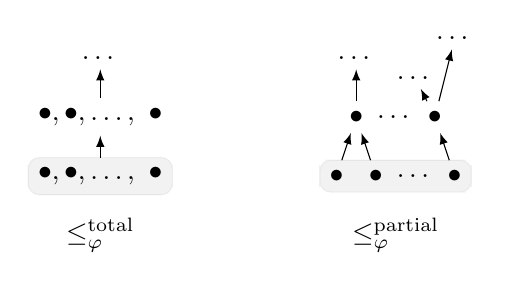
\begin{tikzpicture}
		\node at (0,-0.75){$\le^\totalPre_\phi$};
		\node at (0,0)(0){$\bullet,\bullet,\dots,~\bullet$};
		\node at (0,0.75)(1){$\bullet,\bullet,\dots,~\bullet$};
		\node at (0,1.5)(2){\dots};
		\path[-latex] (0) edge (1)(1) edge (2);
		\fill[draw, opacity=0.05, rounded corners=4]
			(0.south)--
			(0.south west)--
			(0.west)--
			(0.north west)--
			(0.north)--
			(0.north east)--
			(0.east)--
			(0.south east)--
			(0.south);

		\node at (3.75,-0.75){$\le^\partialPre_\phi$};
		\node at (3,0)(0){$\bullet$};
		\node at (3.5,0)(1){$\bullet$};
		\node at (4,0){\dots};
		\node at (4.5,0)(2){$\bullet$};

		\node at (3.25,0.75)(3){$\bullet$};
		\node at (3.75,0.75){\dots};
		\node at (4.25,0.75)(4){$\bullet$};
		
		\node at (3.25,1.5)(5){\dots};
		\node at (4,1.25)(6){\dots};
		\node at (4.5,1.75)(7){\dots};
		\path[-latex] (0) edge (3)(1) edge (3)(2)edge(4)(3)edge(5)(4)edge(6)(4)edge(7);
		\fill[draw, opacity=0.05, rounded corners=4]
			(0.south)--
			(0.south west)--
			(0.west)--
			(0.north west)--
			(0.north)--
			(2.north)--
			(2.north east)--
			(2.east)--
			(2.south east)--
			(2.south)--
			(0.south);	
	\end{tikzpicture}
	\caption{
		A schematic depiction of a total preorder $\le^\totalPre_{\phi}$ 
		and a partial preorder $\le^\partialPre_{\phi}$
		in an r-faithful assignment.
		Bullets stand for interpretations.
		The situation where $w_1\approx^i_\phi w_2$ 
		(depicted by bullets) is illustrated by drawing 
		$w_1$ and $w_2$ on the same level and separating them by a comma,
		while the situation where neither 
		$w_1\le^i_\phi w_2$ nor $w_2\le^i_\phi w_1$ 
		is illustrated by drawing them apart.
		An arrow from interpretation $w_1$ to $w_2$ means that $w_1<^i_\phi w_2$, i.e., lower means strictly more plausible.
		Models of $\phi$ are shaded in light gray. 
	}
	\label{fig:3-revision-rfaithful-schematic}
\end{figure}

An $\L$-assignment $\as$ on interpretations is \emph{r-faithful} if 
$\as$ satisfies properties $\oor{6}$ and $\oor{7}$.
Note that, per the observation in the preceding paragraph, 
if $\as$ is total, then property $\oor{6}$ implies $\oor{5}$.
Thus, a total r-faithful $\L$-assignment $\as$ actually satisfies
property $\oor{5}$ as well.
A schematic illustration of preorders in a total and partial r-faithful 
assignment is given in Figure \ref{fig:3-revision-rfaithful-schematic}.

It is clear from the exposition above that the structural properties $\oor{1-3}$
are separate from properties $\oor{4-7}$, 
in the sense that an assignment $\as$ can satisfy properties $\oor{1-3}$ without 
satisfying properties $\oor{4-7}$.
The two sets of properties also differ in their scope:
properties $\oor{1-3}$ talk about the way in which $\as$ looks,
whereas properies $\oor{4-7}$
about the influence of $\phi$ on $\le_{\phi}$
Nonetheless, it is a longstanding tradition in belief revision to focus 
on r-faithful $\L$-assignments that are also insensitive to syntax,
or, as they are more commonly known, `faithful assignments' \cite{KatsunoM92}, 
since the properties we have introduced separately above 
are commonly bundled together into one package.%
\footnote{
	We add the `r' qualifier in `r-faithful' to distinguish such assignments 
	from faithful assignments specific to other types of belief change, to come.
}
In r-faithful $\L$-assignments the 
relation $\le_{\phi}$ on interpretations is a preorder, either total or partial,
in which models of $\phi$ are 
the $\le_\phi$-minimal, i.e., most plausible, outcomes.
If insensitivity to syntax is added, as it usually is, then the preorder $\le_{\phi}$
depends only on the models of $\phi$.
In this section we will follow common practice in assuming that properties $\oor{5-7}$
are standard, and include them in the representation results,
though gradually, so as to keep apart the intuitions 
around what depends on what.
We will then subject properties $\oor{5-7}$ to more intense scrutiny in Chapter \ref{ch:4}. 

\subsubsection{Revision as choice over outcomes}
We have introduced two facets of an agent keen on revising its beliefs:
on the one hand, a revision operator combines two propositional formulas into a new one, 
reflecting the change in belief; 
on the other hand, possible outcomes are ranked in terms of plausibility. 
We have hinted that the two facets are linked:
here we finally show how they fit together.

The mechanism linking the two facets is that of choice:
forming a new belief amounts to choosing, from a set of feasible outcomes,
the most plausible ones. The feasible outcomes, in this case, are provided
by the new information $\mu$, and plausibility is provided by the preorder on outcomes:
this is revision induced by the plausibility ranking.
Conversely, inferring a plausibility ranking amounts to assuming,
from an observed instance of revision, 
that the outcomes consistent with the result are considered more plausible than the outcomes
that did not make the cut: this is plausibility revealed by revision behavior.
The remainder of this section is devoted to spelling out the details of this picture.

The first direction involves using plausibility rankings 
on outcomes to determine how a belief is revised.
Thus, given an $\L$-assignment $\as$ on interpretations, 
the \emph{$\as$-induced revision operator $\re^\as$} is defined,
for any propositional formulas $\phi$ and $\mu$, 
by taking:
$$
	[\phi\re^\as\mu]\defeq\min_{\le_\phi}[\mu].
$$
The other direction involves reconstructing an agent's plausibility 
ranking over outcomes from its perceived revision behavior:
we can tell what an agent thinks is more likely from the way it
revises its beliefs.
For this, recall that the $\L$-proxy $\px_{1,2}$ of two interpretations $w_1$ and $w_2$
is a propositional formula such that $[\px_{1,2}]=\{w_1,w_2\}$.
We will distinguish between two ways of interpreting revision behavior:
given a propositional belief change operator $\re$ and a propositional formula $\phi$,
the \emph{exhaustive $\re$-revealed plausibility relation $\le^\exh_\phi$} 
and the \emph{exclusive $\re$-revealed plausibility relation $\le^\exc_\phi$} 
are defined, for any interpretations $w_1$ and $w_2$, respectively, as:
\begin{align*}
	w_1\le^\exh_\phi w_2 &~\text{if}~w_1\in[\phi\re\px_{1,2}],\\
	w_1\le^\exc_\phi w_2 &~\text{if}~w_1\in[\phi\re\px_{1,2}]~\text{and}~w_2\notin[\phi\re\px_{1,2}].
\end{align*}
The \emph{exhaustive revealed assignment $\as^\exh$} 
and \emph{exclusive revealed assignment $\as^\exc$} are obtained
by taking $\as^\exh\!\!(\phi)=\le^\exh_\phi$ and $\as^\exc\!\!(\phi)=\le^\exc_\phi$, 
for any propositional formula $\phi$.
The guiding intuition here is that if an agent leans toward 
outcome $w_1$ rather than outcome $w_2$ when it has 
the possibility of holding on to either of them, 
then this must be because the agent considers $w_1$ 
more plausible than $w_2$.
That is, if $[\phi\re\px_{1,2}]=\{w_1\}$,
then in both cases $w_1$ is considered better than $w_2$,
i.e.,
$w_1<^{\exh}_{\phi} w_2$ and $w_1<^{\exc}_{\phi} w_2$.
The difference between the two types of assignments 
lies in how they treat the case when both $w_1$ and $w_2$ are preserved,
i.e., in the case when $[\phi\re\px_{1,2}]=\{w_1,w_2\}$.
The exhaustive assignment assumes that the agent knows 
enough about the two outcomes
(as it were, has exhaustive reasons) 
to conclude that they are equally likely, 
whereas the exclusive assignment merely infers 
that they cannot be compared,
reserving judgment only for the exclusive case when
$w_1$ is strictly better than $w_2$.

Revision by the $\L$-proxy of two interpretations $w_1$ and $w_2$ 
reveals a small piece of the agent's plausibility ranking over interpretations,
namely the relative ranking of $w_1$ and $w_2$. 
Gluing these pieces together, one pair of interpretations at a time,
yields the agent's full plausibility ranking $\le_{\phi}$.
The endgame of this exercise is that we want the revealed plausibility 
relation to serve as a basis for explaining, 
or rationalizing, the revision behavior of the agent,
in the same way that the preference relation of a single agent
in Section \ref{sec:2-choice-functions} explains its choices across various menus.
This is formalized by saying that 
if $\re$ is an $\L$-revision operator and 
$\as$ is an $\L$-assignment on interpretations,
then \emph{$\as$ represents $\re$}
(and \emph{$\re$ is represented by $\as$})
if, for any propositional formulas $\phi$ and $\mu$,
it holds that $[\phi\re\mu] = \min_{\le_\phi}[\mu]$. 

\begin{figure}\centering
	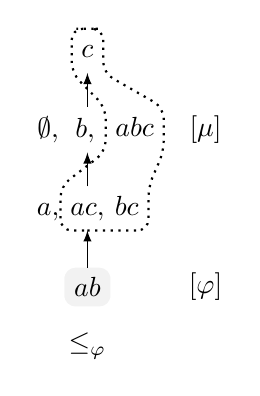
\begin{tikzpicture}
	%% total preorder
	\node at (0,-0.75){$\le_\phi$};
	
	\node at (0,0)(ab){$ab$};
	
	\node at (-0.5,1)(a){$\vphantom{b,}a,$};	
	\node at (0,1)(ac){$\vphantom{b}ac,$};
	\node at (0.5,1)(bc){$bc\vphantom{,}$};
	
	\node at (-0.5,2)(e){$\emptyset,$};
	\node at (0,2)(b){$b,\vphantom{\emptyset}$};
	\node at (0.6,2)(abc){$abc\vphantom{,}$};
	
	\node at (0,3)(c){$\vphantom{b,}c$};
	
	\node at (1.5,0){$\mods{\phi}$};
	\node at (1.5,2){$[\mu]$};
	
	\path[-latex] (ab)edge(ac)(ac)edge(b)(b)edge(c);
	
	\fill[opacity=0.05, rounded corners = 4]
		(ab.south)--
		(ab.south east)--
		(ab.east)--
		(ab.north east)--
		(ab.north)--
		(ab.north west)--
		(ab.west)--
		(ab.south west)--
		(ab.south);
	
	\draw[thick, dotted, rounded corners=4]
		(ac.south)--
		(bc.south)--
		(bc.south east)--
		(bc.east)--
		(bc.north east)--
		(abc.south east)--
		(abc.east)--
		(abc.north east)--
		(c.south east)--
		(c.east)--
		(c.north east)--
		(c.north)--
		(c.north west)--
		(c.west)--
		(c.south west)--
		(abc.north west)--
		(abc.west)--
		(abc.south west)--
		(ac.north west)--
		(ac.west)--
		(ac.south west)--
		(ac.south);
	\end{tikzpicture}
	\caption{
		Total preorder $\le_\phi$, for $[\phi]=\{ab\}$.
		Lower interpretations are better.
		The new information is $\mu = c$,
		and its models are surrounded by the dotted line.
		Revising $\phi$ by $\mu$ amounts to selecting the 
		$\le_\phi$-minimal models of $\mu$.
	}
	\label{fig:3-revision-preorder-operator-interplay}
\end{figure}

\begin{xmpl}{A monopoly on tool use after all?}{3-revision-preorder-operator-interplay}
	We revisit our running revision scenario,
	detailed in 
	Examples \ref{ex:1-revision-motivation}, 
	\ref{ex:3-revision-basic-setup} and \ref{ex:3-revision-R1,3,4}
	with Jane Goodall challenging the primatology status quo.
	This status quo is
	expressed as the propositional formula $\phi$,
	with $[\phi]=\{ab\}$,
	while Jane Goodall's challenge to it
	is the finding $\mu$, with $[\mu]=\{c,ac,bc,abc\}$.
	Suppose that revision among the primatology community 
	is guided by a total r-faithful assignment $\as$
	that assigns to $\phi$ the
	total preorder $\le_\phi$ on interpretations 
	in Figure \ref{fig:3-revision-preorder-operator-interplay}.
	According to the preorder $\le_{\P}$, the state of the world 
	$ab$ is the most likely outcome: this corresponds
	with $ab$ being the unique model of the prior belief $\phi$,
	and is in agreement with properties $\oor{5-7}$.
	Jane Goodall's finding reveals that the only 
	viable outcomes are those consistent with $\mu$
	i.e., the models of $\mu$,
	and that a choice must be made as to which of these model
	will go into the new belief.
	How does the choice take place?
	We have that 
	$[\phi\re^\as\mu] = \min_{\le_\phi}[\mu] = \{ac,bc\}$,
	or, to put it differently,
	$\phi\re^\as\mu\equiv (a\land\lnot b\land c)\lor (\lnot a\land b\land c)$.
	That is, according to $\le_\phi$, the most plausible 
	states of affairs consistent with $\mu$, 
	i.e., the $\le_\phi$-minimal models of $\mu$,
	are $ac$ and $bc$,
	and the rational course of action is to adopt 
	them as the new belief.

	Recall, as well, Louis Leakey's telegram to Jane Goodall
	from Example \ref{ex:1-revision-motivation}:
	``Now we must redefine tool, redefine Man, or accept chimpanzees as humans.''
	Given how we model the problem, 
	Leakey seems to think that the result of revising by $\mu$
	should be either $bc$, 
	i.e., chimpanzees use tools and are not human, 
	but humans don't use tool (redefining tool),
	or $ac$, i.e., chimpanzees and humans use tools, 
	but chimpanzees are human (accepting chimpanzees as humans).
	If we assume that Louis Leakey had the same prior belief $\phi$
	as the rest of the primatology community
	but was revising according to a revision operator $\re^{LL}$,
	then his telegram seems to suggest an inclination to 
	conclude that $ac$ or $bc$ must be the case.
	In other words, narrowing down the choice to only these two outcomes 
	(i.e., to $\px_{ac,bc}\equiv c \land (a\leftrightarrow\lnot b)$),
	then Leakey seems to think that they cannot be distinguished,
	i.e., $[\phi\re^{LL}\px_{ac,bc}]=\{ac,bc\}$.
	In the exhaustive revealed ranking we would then infer 
	that, for Leakey, it holds that $ac\approx^\exh_\phi bc$,
	and the preorder $\le_\phi$ 
	in Figure \ref{fig:3-revision-preorder-operator-interplay}
	is consistent with this attitude,
	whereas in the exclusive revealed ranking we 
	would infer that $ac\not\le^\exc_\phi bc$ 
	and $ac\not\le^\exc_\phi bc$. 
\end{xmpl}

Example \ref{ex:3-revision-preorder-operator-interplay} illustrates
that rankings of outcomes tell us something,
not about the state of the world,
but about what an agent thinks is more likely.
They can be used to guide revision,
or, conversely, they can be reconstructed, piece by piece,
from putative revision behavior.
But what ensures that a revision operator guided by a plausibility
ranking on outcomes is rational?
And how can we guarantee that the revealed rankings add up to 
a coherent whole?
The answer depends entirely on the constraints imposed on the revision 
operator and on the plausibility rankings,
with the representation results below showing that there is 
a close link between the revision postulates $\ppr{1-8}$
and properties $\oor{1-7}$.
The first result shows that leaving out postulate $\ppr{2}$
and enforcing postulate $\ppr{6}$
results in revision policies that are represented 
by total assignments on interpretations that are also insensitive to syntax,
which, we recall, means that $\le_\phi$ satisfies properties $\oor{1-4}$
(i.e., is a total preorder on $\U$),
and that
$[\phi\re\mu]=\min_{\le_\phi}[\mu]$,
for any propositional formulas $\phi$ and $\mu$.
Recall, as well, that the $\L$-proxy of a set $\{w_1,\dots,w_k\}$ of interpretations
is a propositional formula $\px_{1,\dots,k}$ such that 
$[\px_{1,\dots,k}]=\{w_1,\dots,w_k\}$.

\begin{thm}{}{3-revision-repr-total}
	A revision operator $\re$ satisfies postulates 
	$\ppr{1}$ and $\ppr{3-6}$ (i.e., is exhaustive)
	if and only if there exists	an 
	$\L$-assignment $\as$ on interpretations
	that satisfies properties $\oor{1-4}$
	(i.e., is total and insensitive to syntax)
	and represents the operator $\re$.
\end{thm}
\begin{prf*}{}{}%{}{}
	(``$\Leftarrow$'')
	Assume, first, that we are given an $\L$-assignment $\as$ on interpretations
	such that, for any $\phi\in\L$,	$\le_\phi$ satisfies properties $\oor{1-4}$.
	Since the $\as$-induced revision operator $\re^\as$ is
	defined by taking $[\phi\re^\as\mu]\defeq\min_{\le_\phi}[\mu]$, 
	the proof amounts to showing that $\re^\as$ satisfies postulates $\ppr{1-4}$.
	
	Postulate $\ppr{1}$ follows from the fact that 
	$\phi\re^\as\mu$ is a formula whose set of models is, by definition,
	a subset of $[\mu]$. Since $[\mu]$ is a finite set and, by properties $\oor{1-2}$,
	$\le_\phi$ is a pre-order, we then have 
	that $\min_{\le_\phi}[\mu]\neq\emptyset$, if $[\mu]\neq\emptyset$.
	This implies that postulate $\ppr{3}$ is satisfied.
	For postulate $\ppr{4}$ we have that if 
	$\phi_1\equiv\phi_2$, then, by property $\oor{4}$, 
	$\le_{\phi_1}=\le_{\phi_2}$.
	Clearly, then, if we also have that $\mu_1\equiv\mu_2$, 
	then it holds that $\min_{\le_{\phi_1}}[\mu_1]=\min_{\le_{\phi_2}}[\mu_2]$. 
	
	For postulate $\ppr{5}$, take $w_1\in[(\phi\re^\as\mu_1)\land\mu_2]$: this means that 
	$w_1\in\min_{\le_\phi}[\mu_1]\cap[\mu_2]$, and we want to show that 
	$w_1\in\min_{\le_\phi}[\mu_1\land\mu_2]$.
	Suppose, on the contrary, that $w_1\notin\min_{\le_\phi}[\mu_1\land\mu_2]$.
	Since we can derive, from our starting assumption, that $w_1\in[\mu_1\land\mu_2]$,
	it follows that $[\mu_1\land\mu_2]\neq\emptyset$,
	and hence that $\min_{\le_\phi}[\mu_1\land\mu_2]\neq\emptyset$.
	Thus there exists $w_2\in\min_{\le_\phi}[\mu_1\land\mu_2]$;
	since $w_1\notin\min_{\le_\phi}[\mu_1\land\mu_2]$
	we then conclude that $w_2<_\phi w_1$.
	But $w_1$ and $w_2$ are both in $[\mu_1]$ and $w_1\in\min_{\le_\phi}[\mu_1]$,
	which implies that $w_1\le_\phi w_2$. We have arrived at a contradiction,
	and thus $w_1\in\min_{\le_\phi}[\mu_1\land\mu_2]$.
	
	For postulate $\ppr6$, take $w_1\in\min_{\le_\phi}[\phi\re^\as(\mu_1\land\mu_2)]$.
	We want to show that $w_1\in[(\phi\re^\as\mu_1)\land\mu_2]$.
	From the fact that $w_1\in\min_{\le_\phi}[\phi\re^\as(\mu_1\land\mu_2)]$
	we infer that $w_1\in[\mu_2]$,
	so all we have to show is that $w_1\in[\phi\re^\as\mu_1]$.
	Suppose, on the contrary, that $w_1\notin[\phi\re^\as\mu_1]$:
	we now use the assumption that $(\phi\re^\as\mu_1)\land\mu_2$ is consistent 
	to conclude that there exists $w_2\in[(\phi\re^\as\mu_1)\land\mu_2]$,
	which implies that $w_2<_\phi w_1$.
	But, since $w_1\in\min_{\le_\phi}[\phi\re^\as(\mu_1\land\mu_2)]$
	and $w_2\in[\mu_1\land\mu_2]$, it also follows that $w_1\le_\phi w_2$.
	This is a contradiction, and we conclude that $w_1\in[\phi\re^\as\mu_1]$.
	
	(``$\Rightarrow$'')
	Assume, now, that we are given an exhaustive belief change operator $\re$, 
	i.e., one that satisfies postulates $\ppr{1}$ and $\ppr{3-6}$.
	We will show that the exhaustive $\re$-revealed assignment $\as^\exh$ 
	is the assignment we are looking for,
	i.e., $\le^\exh_\phi$ satisfies properties $\oor{1-4}$, for any propositional formula $\phi$,
	and $[\phi\re\mu]=\min_{\le^\exh_\phi}[\mu]$, for any propositional formula $\mu$.
	
	For property $\oor{1}$ (reflexivity), take an interpretation $w$ and 
	the $\L$-proxy $\px_w$ of $w$, i.e., a propositional formula such that $[\px_w]=\{w\}$.
	Notice that, using postulates $\ppr{1}$ and $\ppr{3}$, we can conclude that 
	$[\phi\re\px_w]=\{w\}$. This implies that $w\le^\exh_\phi w$.
	
	For property $\oor{2}$ (transitivity), assume there are interpretations $w_1$, $w_2$
	and $w_3$ such that $w_1\le^\exh_\phi w_2$ and $w_2\le^\exh_\phi w_3$. We want to show that $w_1\le^\exh_\phi w_3$.
	We will do this in two steps. 
	The first step consists in showing that $w_1\in[\phi\re\px_{1,2,3}]$,
	where $\px_{1,2,3}$ is an $\L$-proxy of $\{w_1,w_2,w_3\}$,
	i.e., a propositional formula such that $[\px_{1,2,3}]=\{w_1,w_2,w_3\}$. 
	First, notice that, by postulates $\ppr{1}$ and $\ppr{3}$, we have that 
	$\emptyset\subset[\phi\re\px_{1,2,3}]\subseteq[\px_{1,2,3}]$.
	In other words, $[\phi\re\px_{1,2,3}]$ contains at least one of the interpretations $w_1$,
	$w_2$ and $w_3$. We will do a case analysis to show that $w_1\in[\phi\re\px_{1,2,3}]$.
	
	\emph{Case 1}. If $w_1\in[\phi\re\px_{1,2,3}]$, the conclusion is immediate.
	
	\emph{Case 2}. If $w_2\in[\phi\re\px_{1,2,3}]$, then $(\phi\re\px_{1,2,3})\land\px_{1,2}$ is consistent.
	Using postulates $\ppr{5-6}$ and $\ppr{4}$,
	and keeping in mind that $\px_{1,2,3}\land\px_{1,2}\equiv\px_{1,2}$,
	this implies that:
	\begin{align*}
		(\phi\re\px_{1,2,3})\land\px_{1,2} &\equiv\phi\re(\px_{1,2,3}\land\px_{1,2}) &(\text{by}~\ppr{5-6})\\
		 										     &\equiv\phi\re\px_{1,2}. 		                 &(\text{by}~\ppr{4})
	\end{align*}
	By hypothesis, it holds that $w_1\le^\exh_\phi w_2$, which,
	by the definition of the $\re$-revealed exhaustive ranking, 
	implies that $w_1\in[\phi\re\px_{1,2}]$.
	Using this with the equivalence just derived, we arrive at the conclusion that $w_1\in[\phi\re\px_{1,2,3}]$.
	
	\emph{Case 3}. If $w_3\in[\phi\re\px_{1,2,3}]$,
	we infer that $(\phi\re\px_{1,2,3})\land\px_{2,3}$ is consistent.	
	Using, again, postulates $\ppr{5-6}$ and $\ppr{4}$,
	and keeping in mind that $\px_{1,2,3}\land\px_{2,3}\equiv\px_{2,3}$,
	this implies that:
	\begin{align*}
		(\phi\re\px_{1,2,3})\land\px_{2,3} &\equiv\phi\re(\px_{1,2,3}\land\px_{2,3}) &(\text{by}~\ppr{5-6})\\
		 										     &\equiv\phi\re\px_{2,3}. 		                 &(\text{by}~\ppr{4})
	\end{align*}
	Since $w_2\in[\phi\re\px_{2,3}]$ (because $w_2\le^\exh_\phi w_3$),
	we get that $w_2\in[\phi\re\px_{1,2,3}]$.
	We can now reproduce the reasoning from Case 2 to conclude that $w_1\in[\phi\re\px_{1,2,3}]$.
	
	Rounding up the case analysis, we can conclude that $w_1\in[\phi\re\px_{1,2,3}]$.
	With this in hand, we infer that $(\phi\re\px_{1,2,3})\land\px_{1,3}$ is consistent, 
	and we can apply the same blend of postulates $\ppr{5-6}$ and $\ppr{4}$,
	keeping in mind that $\px_{1,2,3}\land\px_{1,3}\equiv\px_{1,3}$:
	\begin{align*}
		(\phi\re\px_{1,2,3})\land\px_{1,3} &\equiv\phi\re(\px_{1,2,3}\land\px_{1,3}) &(\text{by}~\ppr{5-6})\\
		 										     &\equiv\phi\re\px_{1,3}. 		                 &(\text{by}~\ppr{4})
	\end{align*}
	Since $w_1\in[\phi\re\px_{1,2,3}]$ and $w_1\in[\px_{1,3}]$,
	we conclude that $w_1\in[\phi\re\px_{1,3}]$.
	By the definition of $\le^\exh_\phi$, this implies that $w_1\le^\exh_\phi w_3$.
	
	Property $\oor{3}$ (totality) follows from the fact for any two interpretations $w_1$ and $w_2$,
	there exists an $\L$-proxy $\px_{1,2}$ of $\{w_1,w_2\}$,
	and postulate $\ppr{3}$ guarantees that at least one of $w_1$ and $w_2$ is in $[\phi\re\px_{1,2}]$.
	Property $\oor{4}$ follows by using postulate $\ppr{4}$, i.e., 
	the fact that the definition of $\le^{\exh}_\phi$ 
	is not sensitive in any way to the syntax of $\phi$.
	
	The last thing we have to show is that 
	the exhaustive $\re$-revealed assignments represents $\re$,
	i.e., that $[\phi\re\mu]=\min_{\le^\exh_\phi}[\mu]$, for any propositional formula $\mu$.
	We do this by showing the double inclusion. 
	
	(``$\subseteq$'') 
	Take, first, $w_1\in[\phi\re\mu]$,
	and some arbitrary interpretation $w_2\in[\mu]$.
	Applying postulates $\ppr{5}$ and $\ppr{4}$
	and keeping in mind that, because $[\px_{1,2}]\subseteq[\mu]$,
	it holds that $\mu\land\px_{1,2}\equiv\px_{1,2}$,
	we have that:
	\begin{align*}
		(\phi\re\mu)\land\px_{1,2} &\models\phi\re(\mu\land\px_{1,2})    &(\text{by}~\ppr{5})\\
		 										     &\equiv\phi\re\px_{1,2}. &(\text{by}~\ppr{4})
	\end{align*}
	Since $w_1\in[(\phi\re\mu)\land\px_{1,2}]$, it follows that
	$w_1\in[\phi\re(\mu\land\px_{1,2})]$
	and then that $w_1\in[\phi\re\px_{1,2}]$.
	Thus, $w_1\le^{\exh}_\phi w_2$ and, 
	keeping in mind that $w_2$ was arbitrarily chosen among the models of $\mu$,
	we obtain that $w_1\in\min_{\le^\exh_\phi}[\mu]$.
	
	(``$\supseteq$'') 
	Take, now, $w_1\in\min_{\le^\exh_\phi}[\mu]$.
	We want to show that $w_1\in[\phi\re\mu]$.
	Suppose, on the contrary, that $w_1\notin[\phi\re\mu]$.
	Since, due to our assumption, it follows that $\mu$ is consistent,
	we have, by postulate $\ppr{3}$, that there exists $w_2\in[\phi\re\mu]$.
	Using postulates $\ppr{4}$ and $\ppr{6}$, we have that: 
	\begin{align*}
		\phi\re\px_{1,2} &\equiv\phi\re(\mu\land\px_{1,2})    &(\text{by}~\ppr{4})\\
		 					  &\models(\phi\re\mu)\land\px_{1,2}. &(\text{by}~\ppr{6})
	\end{align*}
	By assumption, we have that $w_1\notin[\phi\re\mu]$, and from this it follows that 
	$w_1\notin[(\phi\re\mu)\land\px_{1,2}]$ and, using the implications just derived,
	it holds that
	$w_1\notin[\phi\re\px_{1,2}]$,
	and hence $w_2<^\exh_\phi w_1$.
	But we also have that $w_1\in\min_{\le^\exh_\phi}[\mu]$ and $w_2\in[\mu]$,
	which implies that $w_1\le^\exh_\phi w_2$.
	We have thus arrived at a contradiction.
\end{prf*}

% Theorem \ref{thm:3-revision-repr-total} says that an exhaustive revision operator $\re$
% (i.e., satisfying postulates $\ppr{1}$ and $\ppr{3-6}$)
% is represented by an assignment $\as$ mapping propositional formulas to total preorders, 
% such that $\re$ coincides with the operator induced by the exhaustive revealed assignment $\as^\exh$.
% Thus, one way of thinking of postulates $\ppr{1}$ and $\ppr{3-6}$ is that they axiomatize 
% a choice function on total preorders $\le_\phi$ on interpretations.
% The preorder $\le_\phi$ can be thought of as a plausibility ranking on
% interpretations and is biased towards the prior beliefs $\phi$, in the sense that 
% it ranks the models of $\phi$ as the most plausible interpretations:
% this is in accord with the intuition that a belief in $\phi$ means that states of affairs
% consistent with $\phi$ are thought to be the most likely candidates for the true state of the world.
% In this context, newly acquired information $\mu$ shifts this perspective
% by providing a different menu of states of affairs that are suitable for belief.
% The choice procedure, as traditionally construed, then forms a new belief by choosing among the models of $\mu$
% the most plausible interpretations according to $\le_\phi$.
% [[MORE on the connections to choice]]

The result of Theorem \ref{thm:3-revision-repr-total} is not exactly new, 
and can be easily extracted from the literature \cite{KatsunoM92};
it is certainly present in Hans Rott's work \cite{Rott01}.
Nonetheless, in many standard presentations 
postulates $\ppr{1}$ and $\ppr{3-6}$ are taken together 
with postulate $\ppr{2}$, creating the impression that the postulates
are inextricably tied together. 
Our purpose here is to separate the postulates
that guarantee the structural properties $\oor{1-3}$ 
of the assignment $\as$ 	
from the postulates that say where the 
models of $\phi$ should be placed in that preorder.
Theorem \ref{thm:3-revision-repr-total} 
allows us to see that these are two distinct issues.

The second result shows that leaving out postulate $\ppr{2}$ 
and enforcing postulates $\ppr{7-8}$ instead of $\ppr{6}$
results in revision policies that are represented by partial assignments on interpretations
that are also insensitive to syntax.
Recall, this means that $\le_\phi$ satisfies properties 
$\oor{1-2}$ (i.e., is a partial preorder on $\U$)
and $\oor{4}$, and that
$[\phi\re\mu]=\min_{\le_\phi}[\mu]$,
for any propositional formulas $\phi$ and $\mu$.

\begin{thm}{}{3-revision-repr-partial}
	A revision operator $\re$ satisfies postulates $\ppr{1}$, $\ppr{3-5}$ and $\ppr{7-8}$ 
	(i.e., is exclusive)
	if and only if there exists	
	an $\L$-assignment $\as$ on interpretations
	that satisfies properties $\oor{1-2}$ and $\oor{4}$
	(i.e., is partial and insensitive to syntax) 
	and represents the operator $\re$.
\end{thm}
\begin{prf*}{}{}%
	(``$\Leftarrow$'')
	Starting from an $\L$-assignment $\as$ on interpretations
	that satisfies properties $\oor{1-2}$ and $\oor{4}$,
	the argument that $\re^\as$ satisfies postulates $\ppr{1}$ and $\ppr{3-5}$ is entirely similar
	to the argument for Theorem \ref{thm:3-revision-repr-total}.
	
	For postulate $\ppr{7}$, we have to show that 
	$\min_{\le_\phi}[\mu_1]=\min_{\le_\phi}[\mu_2]$.
	Take, then, $w_1\in\min_{\le_\phi}[\mu_1]$ and suppose that $w_1\notin\min_{\le_\phi}[\mu_2]$.
	By postulate $\ppr{3}$ we have that $\phi\re^\as\mu_2$ is consistent, 
	which implies that there exists $w_2\in\min_{\le_\phi}[\mu_2]$ such that 
	$w_2<_\phi w_1$.
	By the assumption of $\ppr{7}$, it holds that $\phi\re^\as\mu_2\models\mu_1$,
	from which it follows that $w_2\in[\mu_1]$
	and, since $w_1\in\min_{\le_\phi}[\mu_1]$, it follows that $w_2\not<_\phi w_1$,
	We have arrived, in this way, at a contradiction, and thus we conclude
	that $\phi\re^\as\mu_1\models\phi\re^\as\mu_2$.
	The argument that $\phi\re^\as\mu_2\models\phi\re^\as\mu_1$ is entirely similar.
	Together, these two facts imply that $\phi\re^\as\mu_1\equiv\phi\re^\as\mu_2$.
	
	For postulate $\ppr{8}$, take $w\in\min_{\le_\phi}[\mu_1]\cap\min_{\le_\phi}[\mu_2]$ 
	and suppose that $w\notin\min_{\le_\phi}[\mu_1\lor\mu_2]$.
	By postulate $\ppr{3}$ we have that $\min_{\le_\phi}[\mu_1\lor\mu_2]\neq\emptyset$,
	and thus there exists $w'\in\min_{\le_\phi}[\mu_1\lor\mu_2]$ such that 
	$w'<_\phi w$. Since, by postulate $\ppr{1}$, it holds that $w'\in[\mu_1\lor\mu_2]$,
	we conclude that $w'$ has to be an element of $[\mu_1]$ or of $[\mu_2]$.
	This leads to a contradiction with the fact that $w\in\min_{\le_\phi}[\mu_1]\cap\min_{\le_\phi}[\mu_2]$,
	because from this we are forced to conclude that $w'\not<_\phi w$.
	
	(``$\Rightarrow$'')
	Given a revision operator $\re$ that satisfies postulates $\ppr{1}$, $\ppr{3-5}$ and $\ppr{7-8}$,
	we will show that the exclusive $\re$-induced $\L$-assignment $\as^\exc$ on interpretations 
	is the assignment we are looking for, 
	i.e., $\le^\exc_\phi$ satisfies properties $\oor{1-2}$ and $\oor{4}$, 
	for any propositional formula $\phi$ and, for any 
	propositional formula $\mu$, 
	it holds that $[\phi\re\mu]=\min_{\le^\exc_\phi}[\mu]$. 

	For $\oor{1}$ (reflexivity), note that, by postulates $\ppr{1}$ and $\ppr{3}$,
	it holds, for any interpretation $w$, that $[\phi\re\px_w]=\{w\}$.
	This implies that $w\le^\exc_\phi w$.
	
	To show that $\le^\exc$ satisfies property $\oor{3}$ (i.e., is transitive),
	take interpretations $w_1$, $w_2$ and $w_3$ such that 
	$w_1$, $w_2$ and $w_3$ are pairwise distinct and
	$w_1\le^\exc_\phi w_2$ and $w_2\le^\exc_\phi w_3$. 
	We show, first, that $[\phi\re\px_{1,2,3}]=\{w_1\}$,
	where $\px_{1,2,3}$ is an $\L$-proxy of the set $\{w_1, w_2,w_3\}$,
	i.e., a propositional formula such that $[\px_{1,2,3}]=\{w_1,w_2,w_3\}$.
	To that end, note that, by postulates $\ppr{1}$ and $\ppr{3}$, we have that
	$\emptyset\subset[\phi\re\px_{1,2,3}]\subseteq[\px_{1,2,3}]$.
	Suppose, now, that $w_2\in[\phi\re\px_{1,2,3}]$.
	This means that $w_2\in[(\phi\re\px_{1,2,3})\land\px_{1,2}]$.
	Applying postulates $\ppr{5}$ and $\ppr{4}$ we obtain that:
	\begin{align*}
		(\phi\re\px_{1,2,3})\land\px_{1,2} &\models\phi\re (\px_{1,2,3}\land\px_{1,2}) &(\text{by}~\ppr{5})\\
													 &\equiv\phi\re\px_{1,2}.                        &(\text{by}~\ppr{4}) 
	\end{align*}
	But this implies that $w_2\in[\phi\re\px_{1,2}]$, which is a contradiction,
	since, by hopthesis we have that $w_1\le^\exc_\phi w_2$, which, by the definition of $\le^\exc_\phi$,
	implies that $[\phi\re\px_{1,2}]=\{w_1\}$.
	This shows that $w_2\notin[\phi\re\px_{1,2,3}]$. 
	Applying the same strategy to $[(\phi\re\px_{1,2,3})\land\px_{2,3}]$,
	it follows that $w_3\notin[\phi\re\px_{1,2,3}]$.
	Thus, the only remaining possibility is that $[\phi\re\px_{1,2,3}]=\{w_1\}$.

	With this result in hand, we have that $\phi\re\px_{1,2,3}\models\px_{1,3}$.
	It is straightforward to see that $\phi\re\px_{1,3}\models\px_{1,2,3}$,
	which allows us to apply postulate $\ppr{7}$ and infer that $\phi\re\px_{1,2,3}\equiv\phi\re\px_{1,3}$.
	This means that $[\phi\re\px_{1,3}]=\{w_1\}$ and, by the definition of $\le^\exc_\phi$,
	it follows that $w_1\le^\exc_\phi w_3$.

	For $\oor{4}$ (i.e., insensitivity to the syntax of $\phi$ and $\mu$), the argument is entirely similar 
	to the one given in the proof of Theorem \ref{thm:3-revision-repr-total}.

	Finally, we show that $[\phi\re\mu]=\min_{\le^\exc_\phi}[\mu]$ by double inclusion.

	(``$\subseteq$'') 
	Take, first, $w\in[\phi\re\mu]$ and suppose $w\notin\min_{\le^\exc_\phi}[\mu]$.
	This means that there exists $w'\in\min_{\le^\exc_\phi}[\mu]$ such that $w'<^\exc_\phi w$,
	which in turn implies that $[\phi\re\px_{w,w'}]=\{w'\}$.
	But, by postulates $\ppr{5}$ and $\ppr{4}$, we have that:
	\begin{align*}
		(\phi\re\mu)\land\px_{w,w'} & \models\phi\re(\mu\land\px_{w,w'}) &(\text{by}~\ppr{5})\\
										 & \equiv\phi\re\px_{w,w'}.		   &(\text{by}~\ppr{4})
	\end{align*}
	Thus, since $w\notin[\phi\re\px_{w,w'}]$ but $w\in[\px_{w,w'}]$, it follows that $w\notin[\phi\re\mu]$,
	which is a contradiction.

	(``$\supseteq$'') 
	Take, now, $w\in\min_{\le^\exc_\phi}[\mu]$ and suppose $w\notin[\phi\re\mu]$,
	and an arbitrary $w_i\in[\mu]$. Since $w\in\min_{\le^\exc_\phi}[\mu]$,
	it cannot be the case that $w_i<^\exc_\phi w$, which implies that 
	$w\in[\phi\re\px_{w,w_i}]$:
	to see why, suppose that $w\notin[\phi\re\px_{w,w_i}]$;
	by postulates $\ppr{1}$ and $\ppr{3}$, $[\phi\re\px_{w,w_i}]$ 
	needs to be a non-empty subset 
	of $[\px_{w,w_i}]$, 
	and this implies that $[\phi\re\px_{w,w_i}]=\{w_i\}$,
	hence $w_i<^{\exc}_{\phi}w$.
	Applying postulate $\ppr{8}$ for every $w_i\in[\mu]$, 
	and keeping in mind that $\bigvee_{w_i\in[\mu]}\px_{w,w_i}\equiv\mu$,
	we obtain that:
	\begin{align*}
		\bigwedge_{w_i\in[\mu]}(\phi\re\px_{w,w_i}) 		& 
		\models\phi\re(\bigvee_{w_i\in[\mu]}\px_{w,w_i}) 	&
		(\text{by}~\ppr{5})										\\
																& 
		\equiv\phi\re\mu.                                       &
		(\text{by}~\ppr{4})										\\ 
	\end{align*}
	It then follows that $w\in[\phi\re\mu]$.
\end{prf*}

Theorems \ref{thm:3-revision-repr-total} and \ref{thm:3-revision-repr-partial}
make it official:
the behavior of an agent revising its beliefs according to postulates $\ppr{1}$, $\ppr{3-5}$
and either postulate $\ppr{6}$ or postulates $\ppr{7-8}$,
can be rationalized using preorders on outcomes, such that the outcomes the agent 
ends up accepting as part of its revised belief are the most plausible outcomes
consistent with the new information.
It is as if the new information provides a menu of allowable alternatives, 
and the agent chooses the best outcomes from this menu to believe.

Indeed, the similarity of this perspective with the rational choice framework for a single agent
presented in Section \ref{sec:2-choice-functions} runs deeper,
as an $\L$-revision operator $\re$ can be seen to be a choice function
over the set $\U$ of interpretations, 
with $[\mu]$ as the choice set.
Contemplation of postulates $\ppr{1}$, $\ppr{3}$ and $\ppr{5-6}$ quickly reveals 
the parallel to the axioms for choice functions:
viewed semantically, postulates $\ppr{1}$ and $\ppr{3}$ say that 
$[\phi\re\mu]\subseteq[\mu]$ and that, if $[\mu]\neq\emptyset$, 
then $[\phi\re\mu]\neq\emptyset$,
which coincides with properties $\ooch{1}$ and $\ooch{2}$, 
respectively, of a choice function.
Since these properties can be taken to be constitutive of a 
choice function, we could even prove a mini-result saying that any 
revision operator satisfying postulates $\ppr{1}$ and $\ppr{3-4}$
is equivalent to a choice function on the set $\U$ of interpretations
satisfying properties $\ooch{1-2}$: this is sufficiently obvious, however,
to leave it as an observation.

Moving further, it can be seen that postulates $\ppr{5}$ and $\ppr{6}$ 
coincide with properties $\ooch{3}$ and $\ooch{5}$, respectively.
Correspondingly, deviations from them are similar in spirit:
Examples \ref{ex:3-revision-R5,6} and \ref{ex:3-revision-R8},
showing agents that revise in ways inconsistent with postulates $\ppr{5-8}$
are, on a close reading, entirely consonant with Example \ref{ex:2-choice-props},
showing an agent that chooses in ways inconsistent with properties $\ooch{3-4}$.
The parallel is entirely justified, as both types of agents exhibit 
the same kind of pathological behavior when choosing among a set menu:
the doctors in Examples \ref{ex:3-revision-R5,6} and \ref{ex:3-revision-R8} are just choosing 
odd things to believe, or, to be more precise, they revise in ways that are not 
immediately rationalizable by unique plausibility relations on outcomes.
In the same spirit, Theorem \ref{thm:3-revision-repr-total} can be seen 
as a direct analogue of Theorem \ref{thm:2-choice-repr}.
Postulate $\ppr{4}$ has no analogue in the choice framework, since no distinction 
is made there between syntax and semantics.

We can see unfolding here 
a point that has been made before in belief change
\cite{Rott92,Schulte99,Rott01,Bonanno09,Arlo-CostaP10}, 
namely that the choice perspective 
is integral to the workings of a revision operator.
And, while we will want to take up this point and explore it further,
it is important to not be too carried away by its significance.
We certainly do not want to suggest that either 
properties $\ooch{1-5}$ or postulates $\ppr{1}$ and $\ppr{3-8}$
uniquely characterize rational choice or rational belief change,
since examples to the contrary are readily available 
\cite{Sen77,Olsson03,Kahneman11}: rationality, as we have mentioned before, 
comes in many flavors, and what is rational in one type of situation 
may not be rational in another.
We can thus presume that the properties covered
so far in Section \ref{sec:2-choice-functions} and in the present section 
touch on only a very small part of 
the whole gamut of rational behavior,
and, inde. 
So, while, we do not want to give this particular formulation 
undue weight, we do want to use the broader implication, 
i.e., that belief change is a type of change, 
to explore the variety of change procedures 
that could count as rational.

Along these lines, we can start thinking of the role of postulate $\ppr{2}$
in the lineup of desirable revision postulates.
One thing that emerges from
Theorems \ref{thm:3-revision-repr-total} and \ref{thm:3-revision-repr-partial} 
is that postulates $\ppr{1}$ and $\ppr{3-5}$,
together with either postulate $\ppr{6}$ or postulates $\ppr{7-8}$,
regulate only the structural properties of the preorder $\le_{\phi}$ 
in an assignment, 
and say nothing about how the prior information $\phi$ 
biases $\le_{\phi}$, 
i.e., about the position of the models of $\phi$ in $\le_\phi$.
This latter aspect, as we will see in Theorems \ref{thm:3-revision-repr-R2-total}
and \ref{thm:3-revision-repr-R2-partial}, 
is traditionally enforced through postulate $\ppr{2}$.
For these results keep in mind 
that an $\L$-proxy of a pair 
$\{w_1,w_2\}$ of interpretations is a propositional formula $\px_{1,2}$ 
such that $[\px_{1,2}]=\{w_1,w_2\}$,
and that the lessons of 
Theorems \ref{thm:3-revision-repr-total} and \ref{thm:3-revision-repr-partial}
are that exhaustive and exclusive $\L$-revision operators 
are guaranteed to be represented by total and partial $\L$-assignments 
on interpretations, respectively.

\begin{thm}{}{3-revision-repr-R2-total}
	If a revision operator $\re$ satisfies postulates 
	$\ppr{1}$ and $\ppr{3-6}$ (i.e., is exhaustive)
	and $\as$ is an
	$\L$-assignment on interpretations that
	satisfies properties $\oor{1-4}$ (i.e., is total and syntax insensitive) 
	and represents the operator $\re$,
	then 
	$\re$ satisfies postulate $\ppr{2}$ if and only if
	$\as$ satisfies properties $\oor{5-7}$
	(i.e., is r-faithful).
\end{thm}
\begin{prf*}{}{}%
	(``$\Rightarrow$'')
	We start with a revision operator $\re$ satisfies postulates 
	$\ppr{1}$ and $\ppr{3-6}$ and a total, syntax insensitive 
	$\L$-assignment $\as$ on interpretations
	that represents it. 
	Consider, now, a propositional formula $\phi$ and 
	two interpretations $w_1$ and $w_2$ such that 
	$w_1$ and $w_2$ are models of $\phi$.
	Using postulate $\ppr{2}$, we can conclude that $[\phi\re\px_{1,2}]=\{w_1,w_2\}$,
	which, together with the fact that $\le_{\phi}$ is total, 
	implies that $w_1\approx_{\phi} w_2$,
	showing that property $\oor{5}$ is satisfied.
	If $w_1\in[\phi]$ and $w_2\notin[\phi]$, then with postulate $\ppr{2}$ again 
	we conclude that $[\phi\re\px_{1,2}]=\{w_1\}$,
	which implies that $w_1<_{\phi}w_2$, showing that property $\oor{7}$ is satisfied.

	(``$\Leftarrow$'')
	Conversely, we have to show that if $[\phi\land\mu]\neq\emptyset$,
	then $\min_{\le_{\phi}}[\mu]=[\phi\land\mu]$. We can do this by showing the 
	double inclusion.

	(``$\subseteq$'')
	Take $w_1\in\min_{\le_{\phi}}[\mu]$ and suppose $w_1\notin[\phi\land\mu]$.
	Since $w_1\in[\mu]$, by postulate $\ppr{1}$,
	the latter fact implies that $w_1\notin[\phi]$.
	Since $[\phi\land\mu]\neq\emptyset$, there exists an 
	interpretation $w_2\in[\phi\land\mu]$.
	We infer from this that $w_2\in[\phi]$ and, together with property $\oor{7}$,
	that $w_2<_{\phi}w_1$.
	But $w_1\in\min_{\le_{\phi}}[\mu]$, so this creates a contradiction.

	(``$\supseteq$'')
	Take $w_1\in[\phi\land\mu]$ and an arbitrary interpretation $w_2\in[\mu]$.
	Using properties $\oor{5}$ and $\oor{7}$, and keeping in mind that 
	$\le_{\phi}$ is total, we conclude that $w_1 \le_{\phi}w_2$,
	which implies that $w_1\in\min_{\le_{\phi}}[\mu]$.
\end{prf*}

Theorem \ref{thm:3-revision-repr-R2-total} takes care of the case 
when $\re$ satisfies the stronger postulate $\ppr{6}$ and is represented 
by a total assignment.
We can obtain a similar result for the case when $\re$ satisfies the weaker postulates 
$\ppr{7-8}$ instead of $\ppr{6}$, and is represented by a partial assignment.

\begin{thm}{}{3-revision-repr-R2-partial}
	If a revision operator $\re$ satisfies postulates 
	$\ppr{1}$, $\ppr{3-5}$ and $\ppr{7-8}$ (i.e., is exclusive)
	and $\as$ is an
	$\L$-assignment on interpretations that
	satisfies properties $\oor{1-2}$ and $\oor{4}$ 
	(i.e., is partial and syntax insensitive) 
	and represents the operator $\re$,
	then 
	$\re$ satisfies postulate $\ppr{2}$ if and only if
	$\as$ satisfies properties $\oor{6}$ and $\oor{7}$
	(i.e., is r-faithful).
\end{thm}
\begin{prf*}{}{}%
	The proof here follows the same lines as the proof for 
	Theorem \ref{thm:3-revision-repr-R2-total},
	so more intuitions can be gleaned from there.

	(``$\Rightarrow$'')
	If $w_1,w_2\in[\phi]$,
	then using postulate $\ppr{2}$ gives us that $[\phi\re\px_{1,2}]=\{w_1,w_2\}$.
	However, since $\le_{\phi}$ is not guaranteed to be total, we cannot conclude 
	that $w_1\approx_{\phi}w_2$; however, we can conclude that $w_1\not<_{\phi}w_2$
	and $w_2\not<_{\phi}w_1$, which means that property $\oor{6}$ is satisfied.
	If $w_1\in[\phi]$ and $w_2\notin[\phi]$, we obtain using postulate $\ppr{2}$ that 
	$[\phi\re\px_{1,2}]=\{w_1\}$, which implies that $w_1<_{\phi}w_2$, 
	showing that property $\oor{7}$ is satisfied.

	(``$\Leftarrow$'')
	We have to show that if $[\phi\land\mu]\neq\emptyset$,
	then $\min_{\le_{\phi}}[\mu]=[\phi\land\mu]$.
	The proof that $\min_{\le_{\phi}}[\mu]\subseteq[\phi\land\mu]$ 
	is entirely similar as for Theorem \ref{thm:3-revision-repr-R2-total}.
	To show that $[\phi\land\mu]\subseteq\min_{\le_{\phi}}[\mu]$,
	suppose that there exists an interpretation $w_1\in[\phi\land\mu]$
	such that $w_1\notin\min_{\le_{\phi}}[\mu]$.
	This means that there exists $w_2\in\min_{\le_{\phi}}[\mu]$
	such that $w_2<_{\phi}w_1$.
	Using the previous result, we can conclude that $w_2\in[\phi]$.
	Since $w_1\in[\phi]$, this contradicts property $\oor{6}$.
\end{prf*}

Theorems \ref{thm:3-revision-repr-total} and \ref{thm:3-revision-repr-R2-total} 
add the final touches to a variant of revision that makes up the 
standard, received Katsuno-Mendelzon model.
Stitching them together with 
Theorems \ref{thm:3-revision-repr-partial} and \ref{thm:3-revision-repr-R2-partial}
gives us the classical  representation results found in the literature,
the first of which is for total preorders.

\begin{thm}{\cite{KatsunoM92}}{3-revision-repr-km-total}
	A revision operator $\re$ satisfies postulates $\ppr{1-6}$ 
	if and only if
	there exists an $\L$-assignment $\as$ on interpretations
	that satisfies properties $\oor{1-7}$
	(i.e., that is total, syntax insensitive and r-faithful) 
	and that represents the operator $\re$.
\end{thm}

The assignment representing an exhaustive operator $\re$, we know from 
Theorems \ref{thm:3-revision-repr-total},
is the exhaustive $\re$-revealed assignment $\as^{\exh}$,
based on pairwise comparisons of interpretations.
The second result is for partial preorders.

\begin{thm}{\cite{KatsunoM92}}{3-revision-repr-km-partial}
	A revision operator $\re$ satisfies postulates $\ppr{1-5}$ and $\ppr{7-8}$ 
	if and only if
	there exists an $\L$-assignment $\as$ on interpretations
	that satisfies properties $\oor{1-2}$, $\oor{4}$ and $\oor{6-7}$
	(i.e., that is partial, syntax insensitive and r-faithful)
	and that represents the operator $\re$.
\end{thm}

In this case, the assignment representing $\re$ is the exclusive $\re$-revealed assignment.
Theorems \ref{thm:3-revision-repr-km-total} and \ref{thm:3-revision-repr-km-partial} 
gather together the insights of the Katsuno-Mendelzon model:
revision according to the postulates given in this section, 
in either of the variants considered, 
amounts to choosing the best outcomes available, 
according to a ranking on outcomes
that is biased by the agent's belief.

But where do such rankings come from?

\subsubsection{Distance-based revision operators}
In Section \ref{sec:2-distances} we presented a 
general method for computing distances from a propositional
formula $\phi$ to an interpretation $w$,
using two ingredients:
the first is a quasi-distance function $\dd$ between interpretations,
used to generate a tuple $(\dd(v,w))_{v\in[\phi]}$ of distances 
between every model of $\phi$ and $w$,
while the second ingredient is an aggregation function $\agg$ used to
aggregate the values in the tuple $(\dd(v,w))_{v\in[\phi]}$
and generate the $(\dd,\:\agg)$-induced distance 
$\dd^{\agg}(\phi,w)$ from $\phi$ to $w$. 
In this section we want to use this notions to 
rank interpretations relative to a formula $\phi$.
Thus, if $\dd$ is a quasi-distance between interpretations,
$\agg$ is an aggregation function,
$\phi$ is a propositional formula,
the \emph{$(\dd,\:\agg)$-induced ranking $\le^{\dd,\:\agg}_{\phi}$}
is defined,
for any two interpretations $w_1$, $w_2$,
as follows:
$$
	w_1 \le^{\dd,\:\agg}_{\phi}w_2~\text{if}~\dd^{\agg}(\phi,w_1)\le \dd^{\agg}(\phi,w_2).
$$
Intuitively, $w_1$ is considered better than $w_2$ according to $\le^{\dd,\:\agg}_{\phi}$
if $w_1$ is closer to $\phi$ than $w_2$, according to the measures uses.
For this section, where we are focused on techniques used in the existing literature,
we will assume that the aggregation function is $\min$ throughout.
Thus, to rephrase things,
if $\dd$ is a quasi-distance between interpretations,
the $(\dd,\:\min)$-induced ranking $\le^{\dd,\:\min}_{\phi}$ is obtained 
by taking, for any two interpretations $w_1$, $w_2$:
\begin{displaymath}
	w_1\le^{\dd,\:\min}_{\phi} w_2~\text{if}~\min(\dd(v,w_1))_{v\in[\phi]}\le\min(\dd(v,w_2))_{v\in[\phi]}.
\end{displaymath}
In other words, an agent whose prior belief is $\phi$ considers 
interpretation $w_1$ more plausible than $w_2$ 
if the shortest distance between $w_1$ and the models of $\phi$ 
is shorter than the shortest distance between $w_2$ and the models of $\phi$,
i.e., if $w_1$ is overall closer to the models of $\phi$ than $w_2$.
If $\dd$ is a quasi-distance,
the \emph{${(\dd,\:\min)}$-induced assignment $\as^{\dd,\:\min}$} is obtained by taking 
$\as^{\dd,\:\min}\!\!(\phi)=\le_\phi^{\dd,\:\min}$,
for any propositional formula $\phi$.
In the same vein, the \emph{${(\dd,\:\min)}$-induced revision operator $\re^{\dd,\:\min}$} 
is the operator induced by the assignment $\as^{\dd,\:\min}$.
This allows us to generate total, syntax insensitive r-faithful assignments.

\begin{prp}{}{3-revision-d-induced-preorder}
	If $\dd$ is a quasi-distance between interpretations and $\phi$ is a propositional formula, 
	the ${(\dd,\:\min)}$-induced ranking $\le^{\dd,\:\min}_\phi$ 
	satisfies properties $\oor{1-5}$ and $\oor{7}$,
	i.e., $\le^{\dd,\:\min}_\phi$ is total, syntax insensitive and r-faithful.
\end{prp}
\begin{prf*}{}{}%
	Since interpretations in $\le_{\phi}^{\dd,\:\min}$ are ranked based on the $\min$-aggregated distance
	from $\phi$, which in this case is a single number,
	it is straightforward to see that $\le_{\phi}^{\dd,\:\min}$ is a total preorder on interpretations,
	i.e., that $\le_{\phi}^{\dd,\:\min}$ satisfies properties $\oor{1-3}$.
	Since the definition of $\le_{\phi}^{\dd,\:\min}$ depends only on the interpretations,
	$\le_{\phi}^{\dd,\:\min}$ also satisfies property $\oor{4}$.
	Finally, it holds that 
	$\dd^\min(\phi,w) = \min(\dd(v,w))_{v\in[\phi]} = 0$ if and only if
	$w\in[\phi]$, 
	which implies that models of $\phi$ are the $\le_{\phi}^{\dd,\:\min}$-minimal
	elements in $\le_{\phi}^{\dd,\:\min}$,
	i.e., $\le_{\phi}^{\dd,\:\min}$ satisfies properties $\oor{5}$ and $\oor{7}$, for any propositional formula $\phi$.		
\end{prf*}

Proposition \ref{prop:3-revision-d-induced-preorder} 
implies that the $({\dd,\:\min})$-induced assignment $\as^{\dd,\:\min}$ 
is total, r-faithful and syntax insensitive, 
which, by Theorem \ref{thm:3-revision-repr-km-total}, 
implies that the $({\dd,\:\min})$-induced revision operator 
$\re^{\dd,\:\min}$ satisfies postulates $\ppr{1-6}$.

\begin{crl}{}{3-revision-d-induced-operator}
	If $\dd$ is a quasi-distance between interpretations, 
	the $(\dd,\:\min)$-induced revision operator $\re^{\dd,\:\min}$ 
	satisfies postulates $\ppr{1-6}$.
\end{crl}

The operators generated using Hamming distance $\dd_{\hamming}$
and drastic distance $\dd_{\drastic}$,
as presented in Section \ref{sec:2-distances},
are denoted $\re^{\hamming,\:\min}$ and $\re^{\drastic,\:\min}$,
respectively.
We will refer to $\re^{\hamming,:\min}$ as \emph{Dalal's operator},
for historical reasons \cite{Dalal88}, 
and to $\re^{\drastic,\:\min}$ as the \emph{drastic operator}.
Dalal's operator and the drastic operator are intuitive examples
of revision operators that satisfy postulates $\ppr{1-6}$,
but Corollary \ref{cor:3-revision-d-induced-operator} shows us 
that they are just two instances of the much larger framework
of $(\dd,\:\min)$-induced operators.
What these operators all have in common is the choice procedure 
used to select the best outcomes and 
the fact that they are based on total preorders.

To get partial preorders, we use two quasi-distance functions $\dd_{1}$ and $\dd_{2}$,
in addition to the $\min$ aggregation function.
On the basis of this, the \emph{$((\dd_{1},\dd_{2}),\:\min)$-induced ranking $\le^{(\dd_{1},\dd_{2}),\:\min}_\phi$}
on interpretations
is defined, for any interpretations $w_1$ and $w_2$, by taking:
$$
	w_1\le^{(\dd_{1},\dd_{2}),\:\min}_\phi w_2~
	\text{if}~\dd_{1}^{\min}(\phi,w_1)\le\dd_{1}^{\min}(\phi,w_2)~\text{and}~\dd_{2}^{\min}(\phi,w_1)\le\dd_{2}^{\min}(\phi,w_2).
$$
Correspondingly, 
the \emph{$((\dd_{1},\dd_{2}),\:\min)$-induced assignment $\as^{(\dd_{1},\dd_{2}),\:\min}$} 
is obtained by taking $\as^{(\dd_{1},\dd_{2}),\:\min}\!\!(\phi)=\le_\phi^{(\dd_{1},\dd_{2}),\:\min}$,
for any propositional formula $\phi$.
In the same vein, the 
\emph{$((\dd_{1},\dd_{2}),\:\min)$-induced revision operator $\re^{(\dd_{1},\dd_{2}),\:\min}$} 
is the operator induced by the assignment $\as^{(\dd_{1},\dd_{2}),\:\min}$.

\begin{prp}{}{3-revision-(d1,d2)-induced-preorder}
	If $\dd_{1}$ and $\dd_{2}$ are quasi-distances between interpretations and 
	$\phi$ is a propositional formula, the $((\dd_{1},\dd_{2}),\:\min)$-induced 
	ranking $\le^{(\dd_{1},\dd_{2}),\:\min}_\phi$ 
	satisfies properties $\oor{1-2}$, $\oor{4}$, $\oor{6}$ and $\oor{7}$,
	i.e., $\le^{(\dd_{1},\dd_{2}),\:\min}_\phi$ is partial, syntax insensitive 
	and r-faithful.
\end{prp}
\begin{prf*}{}{}%
	It is straightforward to see that the $(\dd_{1},\dd_{2}),\:\min$-induced relation
	$\le^{(\dd_{1},\dd_{2}),\:\min}_\phi$ is 
	a partial preorder on $\U$ that is syntax insensitive and still puts models of $\phi$ on the bottom,
	i.e., that it satisfies properties $\oor{1-2}$, $\oor{4}$, $\oor{6}$ and $\oor{7}$, for any propositional formula $\phi$.
\end{prf*}
Proposition \ref{prop:3-revision-(d1,d2)-induced-preorder} 
implies that the $((\dd_{1},\dd_{2}),\:\min)$-induced assignment 
$\as^{(\dd_{1},\dd_{2}),\:\min}$ is r-faithful,
which, by Theorem \ref{thm:3-revision-repr-km-partial}, 
implies that the $((\dd_{1},\dd_{2}),\:\min)$-induced revision operator 
$\re^{(\dd_{1},\dd_{2}),\:\min}$ satisfies postulates $\ppr{1-5}$ and $\ppr{7-8}$.

\begin{crl}{}{3-revision-(d1,d2)-induced-operator}
	If $\dd_{1}$ and $\dd_{2}$ are quasi-distances between interpretations, 
	the $((\dd_{1},\dd_{2}),\:\min)$-induced revision operator 
	$\re^{(\dd_{1},\dd_{2}),\:\min}$ satisfies postulates $\ppr{1-5}$ and $\ppr{7-8}$.
\end{crl}

An example will clarify the two main approaches.

\begin{figure}\centering
	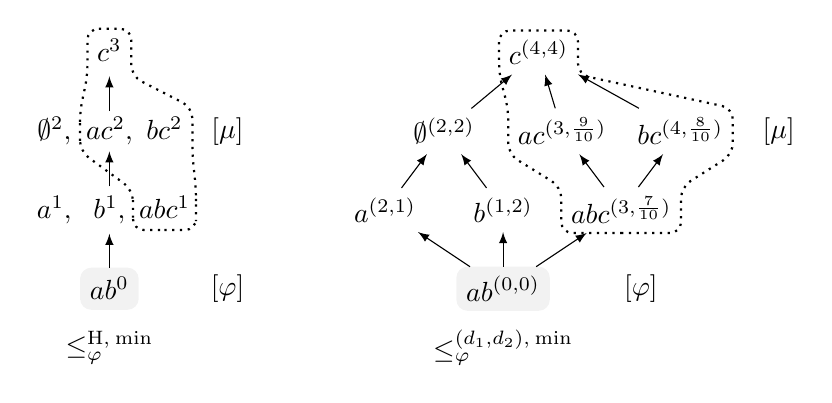
\begin{tikzpicture}
	%% total preorder
	\node at (0,-0.75){$\le^{\hamming,\:\min}_\phi$};
	
	\node at (0,0)(ab){$ab^0$};

	\node at (-0.7,1)(a){$\vphantom{b,}a^1,$};	
	\node at (0,1)(b){$b^1,$};
	\node[inner sep=0.2em] at (0.7,1)(abc){$abc^1\vphantom{,}$};

	\node at (-0.7,2)(e){$\emptyset^2,$};
	\node[inner sep=0.2em] at (0,2)(ac){$\vphantom{\emptyset}ac^2,$};
	\node at (0.7,2)(bc){$bc^2\vphantom{\emptyset,}$};

	\node at (0,3)(c){$\vphantom{b,}c^3$};

	\node at (1.5,0){$\mods{\phi}$};
	\node at (1.5,2){$[\mu]$};

	\path[-latex] (ab)edge(b)(b)edge(ac)(ac)edge(c);
	
	\fill[opacity=0.05, rounded corners = 4]
		(ab.south)--
		(ab.south east)--
		(ab.east)--
		(ab.north east)--
		(ab.north)--
		(ab.north west)--
		(ab.west)--
		(ab.south west)--
		(ab.south);

	\draw[thick, dotted, rounded corners=4]
		(abc.south)--
		(abc.south east)--
		(abc.east)--
		(abc.north east)--
		(bc.south east)--
		(bc.east)--
		(bc.north east)--
		(c.south east)--
		(c.east)--
		(c.north east)--
		(c.north)--
		(c.north west)--
		(c.west)--
		(c.south west)--
		(ac.north west)--
		(ac.west)--
		(ac.south west)--
		(abc.north west)--
		(abc.west)--
		(abc.south west)--
		(abc.south);

	%% partial preorder
	\node at (5,-0.75){$\le^{(\dd_{1},\dd_{2}),\:\min}_\phi$};

	\node at (5,0)(ab){$ab^{(0,0)}$};

	\node at (3.5,1)(a){$a^{(2,1)}$};	
	\node at (5,1)(b){$b^{(1,2)}$};
	\node at (6.5,1)(abc){$abc^{(3,\frac{7}{10})}$};

	\node at (4.25,2)(e){$\emptyset^{(2,2)}$};
	\node at (5.75,2)(ac){$ac^{(3,\frac{9}{10})}$};
	\node at (7.25,2)(bc){$bc^{(4,\frac{8}{10})}$};

	\node at (5.45,3)(c){$c^{(4,4)}$};

	\node at (6.75,0){$\mods{\phi}$};
	\node at (8.5,2){$[\mu]$};
	\path[-latex] 
		(ab)edge(a)(ab)edge(b)(ab)edge(abc)(a)edge(e)
		(b)edge(e)(abc)edge(ac)(abc)edge(bc)(e)edge(c)
		(ac)edge(c)(bc)edge(c);
	
	\fill[opacity=0.05, rounded corners = 4]
		(ab.south)--
		(ab.south east)--
		(ab.east)--
		(ab.north east)--
		(ab.north)--
		(ab.north west)--
		(ab.west)--
		(ab.south west)--
		(ab.south);

	\draw[thick, dotted, rounded corners=4]
		(abc.south)--
		(abc.south east)--
		(abc.east)--
		(abc.north east)--
		(bc.south east)--
		(bc.east)--
		(bc.north east)--
		(c.south east)--
		(c.east)--
		(c.north east)--
		(c.north)--
		(c.north west)--
		(c.west)--
		(c.south west)--
		(ac.north west)--
		(ac.west)--
		(ac.south west)--
		(abc.north west)--
		(abc.west)--
		(abc.south west)--
		(abc.south);
	\end{tikzpicture}
	\caption{
		A total preorder $\le^{\hamming,\:\min}_\phi$ 
		and a partial preorder $\le^{(\dd_{1},\dd_{2}),\:\min}_\phi$. 
		The distances from $\phi$ to each interpretation are written as superscripts next to each interpretation.
		Models of $\phi$ are shaded in gray, models of $\mu$ are in the region bounded by the dotted border. 
	}
	\label{fig:3-revision-dalal-partial}
\end{figure}

\begin{xmpl}{A monopoly on tool use no more}{3-revision-dmin}
	For the last time in this chapter, we look at the revision scenario from 
	Example \ref{ex:3-revision-basic-setup},
	for which $[\phi]=\{ab\}$ and $[\mu]=\{c,ac,bc,abc\}$.
	The preorder $\le_\phi^{\hamming,\:\min}$ generated 
	using Hamming distance and 
	the $\min$ aggregation function is depicted 
	on the left in Figure \ref{fig:3-revision-dalal-partial}.
	According to it we obtain that $[\phi\re^{\hamming,\:\min}\mu]=\min_{\le^{\hamming,\:\min}_\phi}[\mu]=\{abc\}$.
	Consider also 
	two quasi-distances $\dd_{1}$ and $\dd_{2}$ between interpretations that generate
	the partial preorder $\le_\phi^{(\dd_{1},\dd_{2}),\:\min}$ depicted on the right 
	in Figure \ref{fig:3-revision-dalal-partial}. 
	According to it we obtain 
	$[\phi\re^{(\dd_{1},\dd_{2}),\:\min}\mu]=\min_{\le^{(\dd_{1},\dd_{2}),\:\min}_\phi}[\mu]=\{abc\}$,
	which is the same result as for $\re^{\hamming,\:\min}$.

	In both cases, the revision operators arrive at the same conclusion
	that has ultimately prevailed in the primatology community: 
	the minimally disruptive response to Jane Goodall's findings is to 
	hold on to the beliefs that humans use tools and that chimpanzees are a different
	species from humans,
	but to accept that chimpanzees can use tools.
\end{xmpl}

We end this section by returning to a point that was made at its beginning.
The point is that, at least insofar as postulates $\ppr{1-8}$ are concerned,
the type of entity represented by $\phi$ and $\mu$
should be conceived as fluid, hovering somewhere in 
the space of cognitive attitudes an agent can have towards a generic set of issues,
but exclusive to neither of them in particular.
This is seen more clearly through the choice lens, 
embodied by Theorems \ref{thm:3-revision-repr-km-total} and \ref{thm:3-revision-repr-km-partial}):
postulates $\ppr{1-8}$ axiomatize preference maximizing behavior,
i.e., an operation that selects the best alternatives out of a 
set menu, biasing the judgment of what is best on the prior information available; 
this is behavior that is no more exclusive to beliefs than it is to actions
or bundles of goods, and it can be expected to be part of a rational agent's arsenal
in all of these cases.
The general appeal of framing rational behavior in this way
was understood early on in economics 
\cite{Nash1950,Arrow51,Chernoff54,RadnerM54,LuceR57,Hansson68,Sen69,Sen70,Herzberger73},
and is what lies, for Hans Rott, at the root of both theoretical and practical reason:

\begin{quote}
	The constraints [for rational or coherent choice]
	are shown to give rise to corresponding lists of  
	conditions for [\dots] revision and inference operations. 
	I take this to be strong evidence for the unity of 
	theoretical and practical reason, with the principles for 
	the former being special cases of principles for the latter. 
	\cite[p.~214]{Rott92}
\end{quote}

As mentioned before, the moral we want to draw from here 
is not that postulates $\ppr{1-8}$ are the last word in 
what constitutes rational behavior, but that they 
are parts of a larger framework that is worth exploring further.































\section{Update}\label{sec:3-update}
Revision, as we have seen in Section \ref{sec:3-revision},
works by choosing the best outcomes from the ones consistent 
with the new information,
or, in what is the same thing,
by discarding any outcomes from the new information
that are not optimal.
While this selection process makes sense in certain scenarios,
there are cases in which it ends up being too aggressive.

\begin{xmpl}{Keeping up with the humans, as an update task}{3-update-basic-setup}
	Consider the scenario in Example \ref{ex:1-update-motivation}.
	The variables that my automatic assistant keeps track of are 
	whether the temperature is above $15\si{\degree}$ C ($a$),
	whether the Wi-Fi is on after $21{:}00$ ($b$),
	and whether my friend is online after $21{:}00$ ($c$).
	The instructions my assistant is programmed to implement 
	are $\phi=a\land \lnot b$,
	whereas my observed pattern of behavior is represented by the formula 
	$\mu=(b\leftrightarrow c)$.
	The assistant would like to
	modify its list of instructions to accommodate my behavior,
	i.e., to change $\phi$ in accordance with $\mu$.
	In this case, it seems like the sensible answer is 
	to move from $\phi$ to $\phi' = a\land (b \leftrightarrow c)$,
	i.e., maintain temperature above $15\si{\degree}$ C and 
	leave the Wi-Fi on after $21{:}00$
	at exactly those times when my friend is online.
	Note that revision is not the appropriate operation here:
	since $\phi$ and $\mu$ are consistent, a typical revision operator would 
	return $\phi\land\mu\equiv a\land\lnot b\land \lnot c$:
	according to the logic of revision
	my smarthome would infer that, 
	since it is after $21{:}00$ and the	Wi-Fi is turned off, 
	then my friend must be offline.
\end{xmpl}

Example \ref{ex:3-update-basic-setup} illustrates the need for a belief change operator
that retains more information from the new information $\mu$
than a revision operator would normally do,
while still being biased by $\phi$.
The bias towards $\phi$, therefore,
should not be so strong as to render all but the 
absolute closest outcomes as unfeasible.
Update operators were introduced to do justice to 
this intuition \cite{KatsunoM91},
and we will see that they do so by modifying
the way in which models of $\mu$ are chosen 
for the final result.
In the rest of this section we will focus on the mechanics
of update, using the same methodology as the one used for
revision: postulates, preferences over outcomes, 
representation theorems and distances between interpretations.

% Update was originally introduced to model changes 
% in an agent's epistemic state when the state of the world changes,
% rather than when the agent receives new information 
% about a presumably static world \cite{KatsunoM91}.
% The remaining part of this section will employ the same methodology
% methodology to formalize the mechanism involved here.

\subsubsection{Postulates}
Like revision, update is a single-agent belief change operator.
Formally, an \emph{$\L$-update operator $\up$} 
is a function $\up\colon\L\times\L\rightarrow\L$,
taking as input 
two propositional formulas, 
denoted here by $\phi$ and $\mu$,
and standing in for the agent's prior information and the newly acquired 
information, respectively,
and returning a propositional formula,
denoted here by $\phi\up\mu$,
and standing for the agent's posterior information.
As with revision, $\phi$ and $\mu$ are nominally intended to be beliefs,
but in practice can be any of a number of cognitive attitudes an agent
can have toward a set of items.

Recall that a complete formula $\dot{\phi}$ is complete 
if $\dot{\phi}$ has exactly one model.
If $\up$ is an $\L$-update operator, 
the postulates $\up$ is expected to satisfy are, 
for any propositional formulas $\phi$, $\phi_{1}$, $\phi_{2}$,
complete formulas $\dot{\phi}$,
$\mu$, $\mu_{1}$ and $\mu_{2}$,
as follows:

\begin{description}
	\item[($\ppu{1}$)] $\phi\up\mu\models\mu$.
	
	\item[($\ppu{2}$)] If $\phi\models\mu$, then $\phi\up\mu\equiv\phi$.
	
	\item[($\ppu{3}$)] If $\phi$ and $\mu$ are satisfiable, then $\phi\up\mu$ is satisfiable.
	
	\item[($\ppu{4}$)] If $\phi_1\equiv\phi_2$ and $\mu_1\equiv\mu_2$, 
		then $\phi_1\up\mu_1\equiv\phi_2\up\mu_2$.
	
	\item[($\ppu{5}$)] $(\phi\up\mu_1)\land\mu_2\models\phi\up(\mu_1\land\mu_2)$.
	
	\item[($\ppu{6}$)] If $(\dot{\phi}\up\mu_1)\land\mu_2$ is consistent, 
		then $\dot{\phi}\up(\mu_1\land\mu_2)\models(\dot{\phi}\up\mu_1)\land\mu_2$.

	\item[($\ppu{7}$)] If $\phi\up\mu_1\models\mu_2$ and $\phi\up\mu_2\models\mu_1$, 
		then $\phi\up\mu_1\equiv\phi\up\mu_2$.
	
	\item[($\ppu{8}$)] If $\mu\equiv \mu_{1}\lor\mu_{2}$.
		then $(\dot{\phi}\up\mu_1)\land(\dot{\phi}\up\mu_2)\models\dot{\phi}\up\mu$.
	
	\item[($\ppu{9}$)] $(\phi_{1}\lor\phi_{2})\up\mu\equiv(\phi_1\up\mu)\lor(\phi_2\up\mu)$.
\end{description}

As for revision, postulate $\ppu{6}$ implies postulates $\ppu{7}$ and $\ppu{8}$,
and the plan with respect to their use is the same:
postulates $\ppu{7-8}$ are meant to be alternatives to $\ppu{6}$.
An update operator $\up$ is \emph{exhaustive} if it satisfies postulates $\ppu{1-6}$ and $\ppu{9}$,
and \emph{exclusive} if it satisfies postulates $\ppu{1-5}$ and $\ppu{7-9}$.

The numbering of the postulates is slightly different from the usual ordering 
\cite{KatsunoM91}, but the re-numbering is meant to highlight the close connection
to revision.
Indeed, note that postulates $\ppu{1}$ and $\ppu{3-8}$ are
esentially similar to the revision postulates $\ppr{1}$ and $\ppr{3-8}$
(see Section \ref{sec:3-revision}), with the only point of departure 
being that postulates $\ppu{6}$ and $\ppu{8}$ are meant to apply only 
to complete formulas $\dot{\phi}$.
What is more, if $\phi$ is a complete formula,
then postulates $\ppu{1-8}$ are entirely 
equivalent to revision postulates
$\ppr{1-8}$: this is true even for postulate $\ppu{2}$,
since if $\phi$ is complete then 
$\phi\land\mu$ and $\phi$ become equivalent
and the statement that $\phi\models\mu$
is equivalent to the statement that $\phi\land\mu$ is consistent.
This is an observation that has been made before \cite{PeppasNPFKP96}
but is worth stressing, since it provides 
insight into the working of an update operator:
on complete propositional formulas,
update according to postulates $\ppu{1-8}$
is just revision according to postulates $\ppr{1-8}$.

If $\phi$ is not complete, 
then postulates $\ppu{2}$ and $\ppu{9}$
kick in, and can be seen as new additions
to the toolbox of familiar postulates.
In this case postulate $\ppu{2}$ is a weaker version of the revision postulate
$\ppr{2}$, and regulates the way in which the prior information $\phi$
biases the update result.
Postulate $\ppu{9}$ specifies the way in which the update result
can be decomposed in results for more specific parts of the prior information $\phi$,
i.e., formulas $\phi_{1}$ and $\phi_{2}$
such that $\phi_{1}\lor \phi_{2}\equiv \phi$.
Ultimately, repeated application of postulate $\ppu{9}$ makes the result
for $\phi\up\mu$
entirely dependent on the update result for the complete formulas
that imply $\phi$.
More precisely, if $\px_v$ is an $\L$-proxy for the interpretation $v$,
i.e., a propositional formula such that $[\px_v]=\{v\}$,
then postulate $\ppu{9}$ is equivalent to the following postulate, 
applying for any propositional formulas $\phi$ and $\mu$:

\begin{description}
	\item[($\ppu{10}$)] $\phi\up\mu\equiv \bigvee_{v\in[\phi]}(\px_{v}\up\mu)$.
\end{description}

Postulate $\ppu{10}$ shows that $\phi\up\mu$ can be decomposed
in the results for $\px_{v}\up\mu$, for every $v\in[\phi]$. 
We will make extensive use of postulate $\ppu{9}$ and, even more so, 
of its equivalent reformulation $\ppu{10}$, 
in what is to follow.

\begin{xmpl}{Update is not revision}{3-update-postulates}
	For the setting in Example \ref{ex:3-update-basic-setup},
	where $\phi = a\land\lnot b$
	and $\mu=b\leftrightarrow c$,
	we have that $\phi\land\mu$ is consistent,
	but $\phi\not\models\mu$.
	Thus, whereas a revision operator satisfying postulate $\ppr{2}$ 
	would require the result to be $\phi\land\mu$,
	the update postulate $\ppu{2}$ places no constraints in this case.

	Since $[\phi]=\{a,ac\}$, 
	postulate $\ppu{9}$ (or $\ppu{10}$) requires that 
	$\phi\up\mu\equiv(\px_{a}\up\mu)\lor(\px_{ac}\up\mu)$.
\end{xmpl}

As with the revision postulate $\ppr{8}$ in Section \ref{sec:3-revision},
postulate $\ppu{8}$ has also been slightly re-phrased:
normally there would be no reference to $\mu$, 
with $\mu_{1}\lor\mu_{2}$ written instead.
But here, as well, the difference from the usual statement 
is merely stylistic. 
The role of this re-phrasing is only to make life easier
in Chapter \ref{ch:6}.

\subsubsection{Preferences over outcomes}
Postulate $\ppu{9}$, and even more so postulate $\ppu{10}$,
show that what gets chosen in $\phi\up\mu$ is determined 
by what gets chosen in $\px_{v}\up\mu$,
for every $v\in[\mu]$.
Furthermore, update for complete formulas is just revision.
This provides a useful hint for how to model update as a choice
procedure:
we will use an
\emph{$\L_{\comp}$-assignment $\as$ on interpretations}, 
which is a function $\as\colon\L_{\comp}\rightarrow 2^{\U\times\U}$,
taking as input a complete formula $\dot{\phi}$ and returning
a binary relation on interpretations, 
interpreted, as for revision, as a plausibility ranking.
An $\L_{\comp}$ assignment corresponds to 
what has been called in the literature as a \emph{pointwise assignment}
\cite{KatsunoM91}.

As expected, we are keen on $\as$ satisfying some desirable properties,
and the properties we are interested in are as follows, 
for any complete propositional formulas $\dot{\phi}$, $\dot{\phi_{1}}$, $\dot{\phi_{2}}$
and interpretations $w$, $v$, $w_1$ and $w_2$:

\begin{description}
	\item[($\oou{1}$)] $w\le_{\dot{\phi}} w$.
	\item[($\oou{2}$)] If $w_1\le_{\dot{\phi}} w_2$ and $w_2\le_{\dot{\phi}} w_3$, 
		then $w_1\le_{\dot{\phi}} w_3$.
	\item[($\oou{3}$)] $w_1\le_{\dot{\phi}} w_2$ or $w_2\le_{\dot{\phi}} w_1$.
	\item[($\oou{4}$)] If $\dot{\phi_1}\equiv \dot{\phi_2}$, then it holds that if  $w_1\le_{\dot{\phi_1}}w_2$, then $w_1\le_{\dot{\phi_2}}w_2$. 
	\item[($\oou{5}$)] If $[\dot{\phi}]=\{v\}$ and $w\neq v$, then $v<_{\dot{\phi}} w$.
\end{description}

Properties $\oou{1-4}$ are the same as properties $\oor{1-4}$,
except that they are particularized to complete formulas. 
They say, in effect, that $\le_{\dot{\phi}}$ is a preorder (properties $\oou{1-2}$),
additionally total (property $\oou{3}$)
and syntax insensitive (property $\oou{4}$),
for any complete propositional formula $\dot{\phi}$.
Property $\oou{5}$ conveys the same message as properties $\oor{5-7}$:
models of $\dot{\phi}$ are the unique minimal elements in $\le_{\dot{\phi}}$,
but, as $\dot{\phi}$ has only one model,
the distinctions inherent in properties $\oor{5-7}$ are not needed.
We are left, in this case, with the simpler property $\oou{5}$.

\begin{figure}\centering
	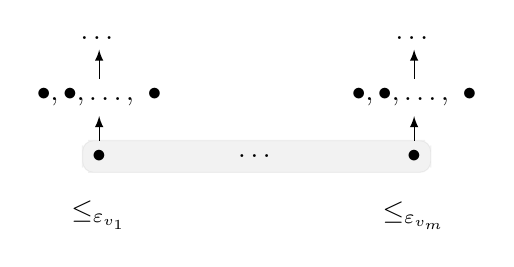
\begin{tikzpicture}
		\node at (0,-0.75){$\le_{\px_{v_{1}}}$};
		\node at (0,0)(01){$\bullet$};
		\node at (0,0.75)(1){$\bullet,\bullet,\dots,~\bullet$};
		\node at (0,1.5)(2){\dots};
		\path[-latex] (01) edge (1)(1) edge (2);
		
		\node at (2,0){\dots};

		\node at (4,-0.75){$\le_{\px_{v_{m}}}$};
		\node at (4,0)(0m){$\bullet$};
		\node at (4,0.75)(1){$\bullet,\bullet,\dots,~\bullet$};
		\node at (4,1.5)(2){\dots};
		\path[-latex] (0m) edge (1)(1) edge (2);

		\fill[draw, opacity=0.05, rounded corners=4]
			(0m.south)--
			(01.south)--
			(01.south west)--
			(01.west)--
			(01.north west)--
			(01.north)--
			(0m.north)--
			(0m.north east)--
			(0m.east)--
			(0m.south east)--
			(0m.south);	
	\end{tikzpicture}
	\caption{
		A schematic depiction of total preorders $\le_{\px_{v_i}}$,
		for $[\phi]=\{v_1,\dots,v_m\}$,
		in a total u-faithful assignment. 
		Bullets stand, as before, for interpretations.
		Each model of $\phi$ (placed in the shaded gray region) 
		generates its own total preorder on interpretations.
	}
	\label{fig:3-update-ufaithful-schematic}
\end{figure}

An $\L_{\comp}$-assignment $\as$ on interpretations is 
\emph{partial} if it satisfies properties $\oou{1-2}$,
\emph{total} if it satisfies properties $\oou{1-3}$,
syntax insensitive if it satisfies property $\oou{4}$
and \emph{u-faithful} if it satisfies property $\oou{5}$.
A schematic illustration of preorders in a total u-faithful
assignment is given in Figure \ref{fig:3-update-ufaithful-schematic}.

\subsubsection{Update as choice over outcomes}
Seeing update as a choice procedure over outcomes
involves putting together the two perspectives introduced
in the previous paragraphs: the logical postulates, on the
one side, and the plausibility rankings on interpretations, on the other.
As with revision, plausibility rankings can be used to guide update,
as well as be inferred from update behavior.

Thus, keeping in mind that
$\px_{v}$ is a propositional formula such that $[\px_{v}]=\{v\}$,
then, given an $\L_{\comp}$-assignment $\as$ on interpretations,
the \emph{$\as$-induced update operator $\up^{\as}$}
is defined, for any propositional formulas $\phi$ and $\mu$,
by taking:
$$
[\phi\up^{\as}\mu] \defeq \bigcup_{v\in[\phi]}\min_{\le_{\px_{v}}}[\mu].
$$
Conversely, given an $\L$-update operator $\up$,
and a complete propositional formula $\dot{\phi}$,
the \emph{exhaustive $\up$-revealed plausibility relation $\le^\exh_{\dot{\phi}}$} 
and the \emph{exclusive $\up$-revealed plausibility relation $\le^\exc_{\dot{\phi}}$} 
are defined, for any interpretations $w_1$ and $w_2$, respectively, as:
\begin{align*}
	w_1\le^\exh_{\dot{\phi}} w_2 &~\text{if}~w_1\in[\dot{\phi}\re\px_{1,2}],\\
	w_1\le^\exc_{\dot{\phi}} w_2 &~\text{if}~w_1\in[\dot{\phi}\re\px_{1,2}]~\text{and}~w_2\notin[\dot{\phi}\re\px_{1,2}].
\end{align*}
The \emph{exhaustive revealed $\L_{\comp}$-assignment $\as^\exh$} 
and \emph{exclusive revealed $\L_{\comp}$-assignment $\as^\exc$} are obtained
by taking $\as^\exh\!\!(\dot{\phi})=\le^\exh_{\dot{\phi}}$ and $\as^\exc\!\!(\dot{\phi})=\le^\exc_{\dot{\phi}}$, 
for any complete propositional formula $\dot{\phi}$.
The guiding intuition here is the same as for the exhaustive and exclusive revealed
assignments in revision.

\begin{figure}\centering
	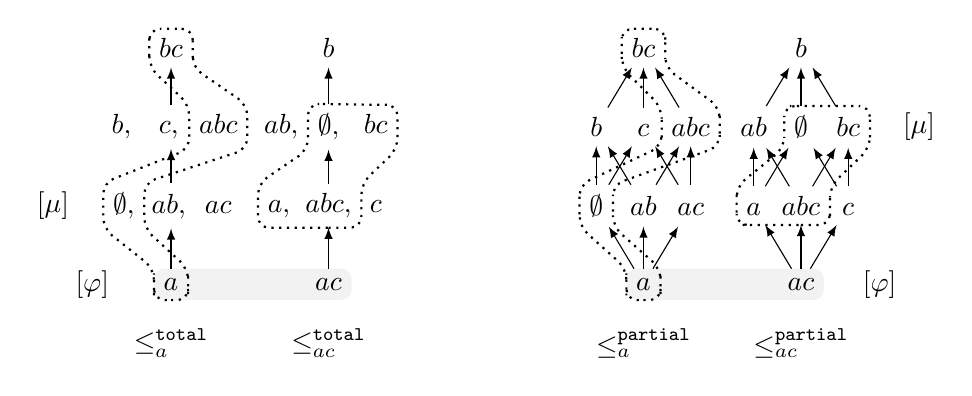
\begin{tikzpicture}
		%% Total preorders
		%% first preorders
		\node at (0,-0.75){$\le^{\mathtt{total}}_{a}$};

		\node at (0,0)(a1){$a$};

		\node at (-0.6,1)(e){$\emptyset,$};
		\node at (0,1)(ab){$ab,\vphantom{\emptyset}$};
		\node at (0.6,1)(ac){$ac\vphantom{\emptyset,}$};
	
		\node at (-0.6,2)(b){$b,\vphantom{b}$};	
		\node at (0,2)(c){$c,\vphantom{b}$};
		\node at (0.6,2)(abc){$abc\vphantom{,}$};		

		\node at (0,3)(bc){$bc$};

		% \node at (1.5,0){$\mods{\phi}$};
		% \node at (1.5,2){$[\mu]$};
	
		\path[-latex] (a1) edge (ab)(ab)edge(c)(c)edge(bc);
		
		\draw[thick, dotted, rounded corners=4]
			(a1.south)--
			(a1.south east)--
			(a1.east)--
			(a1.north east)--
			(e.south east)--
			(e.east)--
			(e.north east)--
			(abc.south east)--
			(abc.east)--
			(abc.north east)--
			(bc.south east)--
			(bc.east)--
			(bc.north east)--
			(bc.north)--
			(bc.north west)--
			(bc.west)--
			(bc.south west)--
			(abc.north west)--
			(abc.west)--
			(abc.south west)--
			(e.north west)--
			(e.west)--
			(e.south west)--
			(a1.north west)--
			(a1.west)--
			(a1.south west)--
			(a1.south);

		%% Second preorder
		\node at (2,-0.75){$\le^{\mathtt{total}}_{ac}$};

		\node at (2,0)(ac1){$ac$};

		\node at (1.4,1)(a){$a,\vphantom{b,}$};
		\node at (2,1)(abc){$abc,$};
		\node at (2.6,1)(c){$c\vphantom{b,}$};
	
		\node at (1.4,2)(ab){$ab,$};
		\node at (2,2)(e){$\emptyset,$};	
		\node at (2.6,2)(bc){$bc\vphantom{,}$};		

		\node at (2,3)(b){$b$};

		\node at (-1,0){$\mods{\phi}$};
		\node at (-1.5,1){$[\mu]$};
	
		\path[-latex] (ac1) edge (abc)(abc)edge(e)(e)edge(b);
		
		\draw[thick, dotted, rounded corners=4]
			(abc.south)--
			(abc.south east)--
			(abc.east)--
			(abc.north east)--
			(bc.south east)--
			(bc.east)--
			(bc.north east)--
			(bc.north)--
			(e.north)--
			(e.north west)--
			(e.west)--
			(e.south west)--
			(a.north west)--
			(a.west)--
			(a.south west)--
			(a.south)--
			(abc.south);
		\fill[opacity=0.05, rounded corners=4]
			(a1.south)--
			(ac1.south)--
			(ac1.south east)--
			(ac1.east)--
			(ac1.north east)--
			(ac1.north)--
			(a1.north)--
			(a1.north west)--
			(a1.west)--
			(a1.south west)--
			(a1.south);


		%%%%%%%%%%%%%%%%%%%%%
		%% Partial preorders
		%% first preorder

		\node at (6,-0.75){$\le^{\mathtt{partial}}_{a}$};

		\node at (6,0)(a1){$a$};

		\node at (5.4,1)(e){$\emptyset$};
		\node at (6,1)(ab){$ab\vphantom{\emptyset}$};
		\node at (6.6,1)(ac){$ac\vphantom{\emptyset}$};
	
		\node at (5.4,2)(b){$b\vphantom{b}$};	
		\node at (6,2)(c){$c\vphantom{b}$};
		\node at (6.6,2)(abc){$abc$};		

		\node at (6,3)(bc){$bc$};

		% \node at (1.5,0){$\mods{\phi}$};
		% \node at (1.5,2){$[\mu]$};
	
		\path[-latex] 
			(a1)edge(e)(a1)edge(ab)(a1)edge(ac) 
			(e)edge(b)(e)edge(c)
			(ab)edge(b)(ab)edge(abc)
			(ac)edge(c)(ac)edge(abc)
			(b)edge(bc)(abc)edge(bc)(c)edge(bc);
		
		\draw[thick, dotted, rounded corners=4]
			(a1.south)--
			(a1.south east)--
			(a1.east)--
			(a1.north east)--
			(e.south east)--
			(e.east)--
			(e.north east)--
			(abc.south east)--
			(abc.east)--
			(abc.north east)--
			(bc.south east)--
			(bc.east)--
			(bc.north east)--
			(bc.north)--
			(bc.north west)--
			(bc.west)--
			(bc.south west)--
			(abc.north west)--
			(abc.west)--
			(abc.south west)--
			(e.north west)--
			(e.west)--
			(e.south west)--
			(a1.north west)--
			(a1.west)--
			(a1.south west)--
			(a1.south);

		%% Second preorder
		\node at (8,-0.75){$\le^{\mathtt{partial}}_{ac}$};

		\node at (8,0)(ac1){$ac$};

		\node at (7.4,1)(a){$a\vphantom{b}$};
		\node at (8,1)(abc){$abc$};
		\node at (8.6,1)(c){$c\vphantom{b}$};

		\node at (7.4,2)(ab){$ab\vphantom{\emptyset}$};
		\node at (8,2)(e){$\emptyset$};	
		\node at (8.6,2)(bc){$bc\vphantom{\emptyset}$};		

		\node at (8,3)(b){$b$};

		\node at (9,0){$\mods{\phi}$};
		\node at (9.5,2){$[\mu]$};
	
		\path[-latex] 
			(ac1)edge(a)(ac1) edge (abc)(ac1)edge(c)
			(a)edge(ab)(a)edge(e)
			(abc)edge(ab)(abc)edge(bc)
			(c)edge(e)(c)edge(bc)
			(ab)edge(b)(e)edge(b)(bc)edge(b);
		
		\draw[thick, dotted, rounded corners=4]
			(abc.south)--
			(abc.south east)--
			(abc.east)--
			(abc.north east)--
			(bc.south east)--
			(bc.east)--
			(bc.north east)--
			(bc.north)--
			(e.north)--
			(e.north west)--
			(e.west)--
			(e.south west)--
			(a.north west)--
			(a.west)--
			(a.south west)--
			(a.south)--
			(abc.south);
		\fill[opacity=0.05, rounded corners=4]
			(a1.south)--
			(ac1.south)--
			(ac1.south east)--
			(ac1.east)--
			(ac1.north east)--
			(ac1.north)--
			(a1.north)--
			(a1.north west)--
			(a1.west)--
			(a1.south west)--
			(a1.south);
		\end{tikzpicture}
	\caption{
		Total and partial preorders 
		$\le^{\mathtt{total}}_{\px_{v}}$ 
		and
		$\le^{\mathtt{partial}}_{\px_{v}}$,
		for $[\phi]=\{a,ac\}$
		and $v\in[\phi]$,
		assigned by a total u-faithful assignment $\as^{\mathtt{total}}$
		and a partial u-faithful assignment $\as^{\mathtt{partial}}$,
		respectively.
		Models of $\phi$ are in the shaded gray regions.
		The new information is $\mu$,
		with $[\mu]=\{\emptyset,a,bc,abc\}$.
		The result of updating $\phi$ by $\mu$
		using the assignment $\as^{\mathtt{total}}$ amounts to taking
		the best models of $\mu$ from the preorders associated to 
		each model of $\phi$,
		i.e., from $\le^{\mathtt{total}}_{a}$ and from 
		$\le^{\mathtt{total}}_{ac}$.
		The same strategy applies to $\as^{\mathtt{partial}}$.
	}
	\label{fig:3-update-preorder-operator-interplay}
\end{figure}	

\begin{xmpl}{Keeping up with the humans, using assignments}{3-update-preorder-operator-interplay}
	For the setting in Example \ref{ex:3-update-basic-setup},
	with 
	$[\phi]=\{a,ac\}$ and $[\mu]=\{\emptyset,a,bc,abc\}$,
	consider two assignments:
	a total r-faithful assignment $\as^{\mathtt{total}}$
	and a partial r-faithful assignment $\as^{\mathtt{partial}}$,
	generating the preorders
	$\le^{\mathtt{total}}_{\px_{v}}$ 
	and
	$\le^{\mathtt{partial}}_{\px_{v}}$
	in Figure \ref{fig:3-update-preorder-operator-interplay},
	for $v\in[\phi]$.
	These assignments generate the update operators
	$\up^{\mathtt{total}}$ and $\up^{\mathtt{partial}}$,
	respectively,
	according to which:
	\begin{align*}
		[\phi\up^{\mathtt{total}}\mu] 												   	&
		=\min_{\le^{\mathtt{total}}_{a}}[\mu]\cup\min_{\le^{\mathtt{total}}_{ac}}[\mu] 	\\
																						   &
		= \{a,abc\}\\
		&= \min_{\le^{\mathtt{partial}}_{a}}[\mu]\cup\min_{\le^{\mathtt{partial}}_{ac}}[\mu]\\
		&=[\phi\up^{\mathtt{partial}}\mu].
	\end{align*}

	Conversely, to find out the agent's ranking of, say, outcomes $b$ and $c$,
	if its initial belief were the complete formula $\px_{a}$,
	with $[\px_{a}]=\{a\}$,
	we would look at the result of $\px_{a}\up\px_{b,c}$.
	Supposing that the result is 
	$[\px_{a}\up\px_{b,c}]=\{b,c\}$,
	then according to the exhaustive $\up$-revealed $\L_{\comp}$-assignment,
	we would conclude that $b\approx^{\exh}_{\px_{a}} c$,
	whereas according to the exclusive $\up$-revealed $\L_{\comp}$-assignment
	we would conclude that neither $b\le^{\exc}_{\px_{a}} c$ nor
	$c\le^{\exc}_{\px_{a}} b$.
	These results are in accordance with
	$\le^{\mathtt{total}}_{\px_{a}}$ 
	and
	$\le^{\mathtt{partial}}_{\px_{a}}$
	as in Figure \ref{fig:3-update-preorder-operator-interplay}.
\end{xmpl}

If $\up$ is an $\L$-update operator
and $\as$ is an $\L_{\comp}$-assignment on interpretations,
then \emph{$\as$ represents $\up$}
(and \emph{$\up$ is represented by $\as$})
if, for any propositional formulas $\phi$ and $\mu$, it holds that 
$[\phi\up\mu]=\bigcup_{v\in[\phi]}\min_{\le_{\px_{v}}}[\mu]$.

As with revision, we obtain two representation results 
for update operators satisfying either postulates $\ppu{1-6}$ and $\ppu{9}$,
or postulates $\ppu{1-5}$, $\ppu{7-9}$,
one for total preorders and one for partial preorders.
The first result is in terms of total preorders

\begin{thm}{\cite{KatsunoM91}}{3-update-repr-km-total}
	An update operator $\up$ satisfies postulates $\ppu{1-6}$ and $\ppu{9}$ 
	(i.e., is exhaustive)
	if and only if
	there exists an 
	$\L_{\comp}$-assignment $\as$ on interpretations
	that satisfies properties $\oou{1-5}$
	(i.e., is total, syntax insensitive and u-faithful)
	and that represents the operator $\up$.
\end{thm}
\begin{prf*}{}{}%
	The $\L_{\comp}$-assignment representing $\up$ is exactly 
	the $\up$-revealed exhaustive assignment $\as^{\exh}$, 
	and the proof that it satisfies properties $\oou{1-5}$
	and that $[\dot{\phi}\up\mu] = \min_{\le^{\exh}_{\dot{\phi}}}[\mu]$,
	for any formula $\mu$ and complete formula $\dot{\phi}$,
	is essentially similar to the proof for the exhaustive
	revealed assignment of a revision operator 
	(see Theorems \ref{thm:3-revision-repr-total} and \ref{thm:3-revision-repr-R2-total}).
	For the last step, i.e., showing that 	
	$[\phi\up\mu]=\bigcup_{v\in[\phi]}\min_{\le^{\exh}_{\px_{v}}}[\mu]$,
	postulate $\ppu{9}$ (or, more precisely, postulate $\ppu{10}$) is used.
\end{prf*}

The accompanying result trades postulate $\ppu{6}$ for $\ppu{7-8}$
to obtain partial preorders instead of total preorders.

\begin{thm}{\cite{KatsunoM91}}{3-update-repr-km-partial}
	An update operator $\up$ satisfies postulates $\ppu{1-5}$, $\ppu{7-8}$ and $\ppu{9}$ 
	(i.e., is exclusive)
	if and only if
	there exists an 
	$\L_{\comp}$-assignment $\as$ on interpretations
	that satisfies properties $\oou{1-2}$ and $\oou{4-5}$
	(i.e., is partial, syntax insensitive and u-faithful)
	and that represents the operator $\up$.
\end{thm}
\begin{prf*}{}{}%
	The $\L_{\comp}$-assignment representing $\up$ is exactly 
	the $\up$-revealed exclusive assignment $\as^{\exc}$, 
	and the proof that it satisfies properties $\oou{1-2}$ and $\oou{4-5}$
	and that $[\dot{\phi}\up\mu] = \min_{\le^{\exc}_{\dot{\phi}}}[\mu]$,
	for any formula $\mu$ and complete formula $\dot{\phi}$,
	is essentially similar to the proof for the exclusive
	revealed assignment of a revision operator 
	(see Theorems \ref{thm:3-revision-repr-partial} and \ref{thm:3-revision-repr-R2-partial}).
	For the last step, i.e., showing that 	
	$[\phi\up\mu]=\bigcup_{v\in[\phi]}\min_{\le^{\exc}_{\px_{v}}}[\mu]$,
	postulate $\ppu{9}$ (or, more precisely, postulate $\ppu{10}$) is used.
\end{prf*}

As with revision, we can refine the analysis 
by separating postulate $\ppu{2}$ from the rest of the postulates:
what we obtain, then, are update operators represented
by either total or partial $\L_{\comp}$-assignments that are syntax insensitive
but do not, however, satisfy property $\oou{5}$ (i.e., are not u-faithful).
In other words, postulate $\ppu{2}$ regulates, as for revision,
the position of the model of a complete formula $\dot{\phi}$
in $\le_{\dot{\phi}}$ and its absence means that this model can
be placed anywhere in $\le_{\dot{\phi}}$.

\subsubsection{Total and partial preorders}
Theorems \ref{thm:3-update-repr-km-total} and \ref{thm:3-update-repr-km-partial}
tell us that to obtain update operators that satisfy postulates $\ppu{1-9}$
we must look for ways of generating rankings on interpretations.
These rankings are supposed to depend on a single interpretation,
so the tried and tested method of using a quasi-distance $\dd$ 
together with an aggregation function $\agg$
works here smoothly (see Section \ref{sec:2-distances}). 
As for revision, we will take $\agg$ in this section 
to be the $\min$ aggregation function.
Thus, if $\dd$ is a quasi-distance between interpretations
and $v$, $w_1$ and $w_2$ are interpretations, the
$(\dd,\:\min)$-induced ranking $\le^{\dd,\:\min}_{\px_{v}}$
is obtained by taking:
$$
	w_1\le^{\dd,\:\min}_{\px_{v}} w_2~\text{if}~\dd(v,w_1)\le \dd(v,w_2).
$$
If $\dd$ is a quasi-distance,
the \emph{${(\dd,\:\min)}$-induced assignment $\as^{\dd,\:\min}$} is obtained,
similarly as for revision, by taking 
$\as^{\dd,\:\min}\!\!(\dot{\phi})=\le_{\dot{\phi}}^{\dd,\:\min}$,
for any complete propositional formula $\dot{\phi}$.
The \emph{${(\dd,\:\min)}$-induced $\L$-update operator $\up^{\dd,\:\min}$} 
is the operator induced by the $\L_{\comp}$-assignment $\as^{\dd,\:\min}$.
The assignments that are generated in this way turn out to be 
total, syntax insensitive and u-faithful.

\begin{prp}{}{3-update-d-induced-preorder}
	If $\dd$ is a quasi-distance between interpretations 
	and $\dot{\phi}$ is a complete propositional formula, 
	the ${(\dd,\:\min)}$-induced ranking $\le^{\dd,\:\min}_{\dot{\phi}}$ 
	satisfies properties $\oor{1-5}$, 
	i.e., $\le^{\dd,\:\min}_{\dot{\phi}}$ is total,
	syntax insensitive and u-faithful.
\end{prp}
\begin{prf*}{}{}%
	Entirely similar to the proof for Proposition \ref{prop:3-revision-d-induced-preorder}.
\end{prf*}

Proposition \ref{prop:3-update-d-induced-preorder} 
implies that the $({\dd,\:\min})$-induced assignment $\as^{\dd,\:\min}$ 
is total, u-faithful and syntax insensitive, 
which, by Theorem \ref{thm:3-update-repr-km-total}, 
implies that the $({\dd,\:\min})$-induced update operator 
$\up^{\dd,\:\min}$ satisfies postulates $\ppu{1-9}$.

\begin{crl}{}{3-update-d-induced-operator}
	If $\dd$ is a quasi-distance between interpretations, 
	the $(\dd,\:\min)$-induced update operator $\up^{\dd,\:\min}$ 
	satisfies postulates $\ppu{1-6}$ and $\ppu{9}$.
\end{crl}

The operators generated using Hamming distance $\dd_{\hamming}$
and drastic distance $\dd_{\drastic}$
are denoted $\up^{\hamming,\:\min}$ and $\up^{\drastic,\:\min}$,
respectively.
We will refer to $\up^{\hamming,\:\min}$ as \emph{Forbus's operator} \cite{Forbus89}, 
and to $\up^{\drastic,\:\min}$ as the \emph{drastic update operator}.

Since any update operator that satisfies postulates $\ppu{1-6}$
also satisfies postulates $\ppu{7-8}$, Forbus's operator and the drastic 
update operator work as examples for both exhaustive and exclusive operators.
To obtain purely exclusive operators we could use the same technique as in 
Section \ref{sec:3-revision}, i.e., employ two quasi-distances $\dd_1$ and $\dd_2$.
However, we will present a different type of operator here.
If $w_1$ and $w_2$ are two interpretations, 
the \emph{symmetric difference $w_1\triangle w_2$ between $w_1$ and $w_2$} is defined as:
$$
	w_1\triangle w_2 = (w_1\setminus w_2)\cup(w_2\setminus w_1).
$$
We have already used the cardinality of the symmetric difference between $w_1$ and $w_2$
to define the Hamming distance between $w_1$ and $w_2$,
but here we will focus on the actual contents of the symmetric difference.
Thus,
if $v$, $w_1$ and $w_2$ are interpretations, the
$\symdiff$-induced ranking $\le^{\symdiff}_{\px_{v}}$
is obtained by taking:
$$
	w_1\le^{\symdiff}_{\px_{v}} w_2~\text{if}~(v\triangle w_1) \subseteq (v\triangle w_2).
$$
If $\dd$ is a quasi-distance,
the \emph{$\symdiff$-induced $\L_{\comp}$-assignment $\as^{\symdiff}$} is obtained,
by taking 
$\as^{\symdiff}\!\!(\dot{\phi})=\le_{\dot{\phi}}^{\symdiff}$,
for any complete propositional formula $\dot{\phi}$.
The \emph{$\symdiff$-induced $\L$-update operator $\up^{\symdiff}$},
is the operator induced by the $\L_{\comp}$-assignment $\as^{\symdiff}$.
The $\symdiff$-induced $\L$-update operator $\up^{\symdiff}$
is also called Winslett's operator \cite{Winslett05}.

The $\L_{\comp}$-assignment $\as^{\symdiff}$
turns out to be 
partial, syntax insensitive and u-faithful.

\begin{prp}{}{3-update-symdiff-induced-preorder}
	If $\dot{\phi}$ is a complete propositional formula, 
	the $\symdiff$-induced ranking $\le^{\symdiff}_{\dot{\phi}}$ 
	satisfies properties $\oou{1-2}$ and $\oou{4-5}$, 
	i.e., $\le^{\symdiff}_{\dot{\phi}}$ is a partial preorder 
	on interpretations that
	is syntax insensitive and 
	makes the model of $\dot{\phi}$ 
	the $\le^{\symdiff}_{\dot{\phi}}$-minimal element.
\end{prp}
\begin{prf*}{}{}%
	It is straightforward to see that $\le_{\dot{\phi}}^{\symdiff}$ satisfies 
	properties $\oou{1-2}$ and $\oou{4}$. 
	Notice, now, that if $w$ is an interpretation such that $v\neq w$,
	then $v\triangle w\neq\emptyset$, whereas $v\triangle v = \emptyset$.
	Thus, for any $w\neq v$, it holds that 
	$v<^{\symdiff}_{\px_v}w$, which shows that $\le^{\symdiff}_{\px_v}$
	satisfies property $\oou{5}$.
\end{prf*}

Proposition \ref{prop:3-update-symdiff-induced-preorder} 
implies that the $\symdiff$-induced assignment $\as^{\symdiff}$ 
is partial, u-faithful and syntax insensitive, 
which, by Theorem \ref{thm:3-update-repr-km-partial}, 
implies that the $\symdiff$-induced update operator 
$\up^{\symdiff}$ satisfies postulates $\ppu{1-5}$ and $\ppu{7-9}$.

\begin{crl}{}{3-update-symdiff-induced-operator}
	The $\symdiff$-induced update operator $\up^{\symdiff}$ 
	satisfies postulates $\ppu{1-6}$ and $\ppu{9}$.
\end{crl}

\begin{figure}\centering
	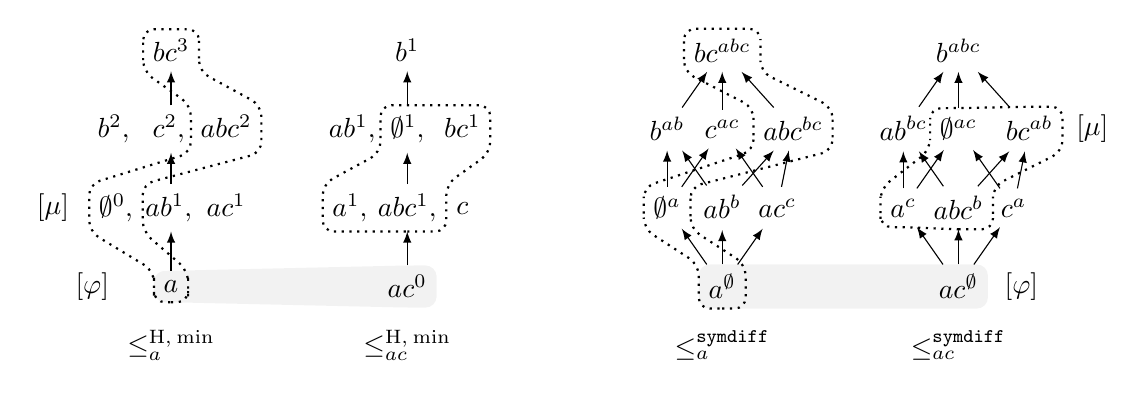
\begin{tikzpicture}
		%% Total preorders
		%% first preorders
		\node at (0,-0.75){$\le^{\hamming,\:\min}_{a}$};

		\node at (0,0)(a1){$a$};

		\node at (-0.7,1)(e){$\emptyset^0,$};
		\node at (0,1)(ab){$ab^1,\vphantom{\emptyset}$};
		\node at (0.7,1)(ac){$ac^1\vphantom{\emptyset,}$};
	
		\node at (-0.7,2)(b){$b^2,\vphantom{b}$};	
		\node at (0,2)(c){$c^2,\vphantom{b}$};
		\node at (0.7,2)(abc){$abc^2\vphantom{,}$};		

		\node at (0,3)(bc){$bc^3$};

		% \node at (1.5,0){$\mods{\phi}$};
		% \node at (1.5,2){$[\mu]$};
	
		\path[-latex] (a1) edge (ab)(ab)edge(c)(c)edge(bc);
		
		\draw[thick, dotted, rounded corners=4]
			(a1.south)--
			(a1.south east)--
			(a1.east)--
			(a1.north east)--
			(e.south east)--
			(e.east)--
			(e.north east)--
			(abc.south east)--
			(abc.east)--
			(abc.north east)--
			(bc.south east)--
			(bc.east)--
			(bc.north east)--
			(bc.north)--
			(bc.north west)--
			(bc.west)--
			(bc.south west)--
			(abc.north west)--
			(abc.west)--
			(abc.south west)--
			(e.north west)--
			(e.west)--
			(e.south west)--
			(a1.north west)--
			(a1.west)--
			(a1.south west)--
			(a1.south);

		%% Second preorder
		\node at (3,-0.75){$\le^{\hamming,\:\min}_{ac}$};

		\node at (3,0)(ac1){$ac^0$};

		\node at (2.3,1)(a){$a^1,\vphantom{b,}$};
		\node at (3,1)(abc){$abc^1,$};
		\node at (3.7,1)(c){$c\vphantom{b,}$};
	
		\node at (2.3,2)(ab){$ab^1,$};
		\node at (3,2)(e){$\emptyset^1,$};	
		\node at (3.7,2)(bc){$bc^1\vphantom{,}$};		

		\node at (3,3)(b){$b^1$};

		\node at (-1,0){$\mods{\phi}$};
		\node at (-1.5,1){$[\mu]$};
	
		\path[-latex] (ac1) edge (abc)(abc)edge(e)(e)edge(b);
		
		\draw[thick, dotted, rounded corners=4]
			(abc.south)--
			(abc.south east)--
			(abc.east)--
			(abc.north east)--
			(bc.south east)--
			(bc.east)--
			(bc.north east)--
			(bc.north)--
			(e.north)--
			(e.north west)--
			(e.west)--
			(e.south west)--
			(a.north west)--
			(a.west)--
			(a.south west)--
			(a.south)--
			(abc.south);
		\fill[opacity=0.05, rounded corners=4]
			(a1.south)--
			(ac1.south)--
			(ac1.south east)--
			(ac1.east)--
			(ac1.north east)--
			(ac1.north)--
			(a1.north)--
			(a1.north west)--
			(a1.west)--
			(a1.south west)--
			(a1.south);


		%%%%%%%%%%%%%%%%%%%%%
		%% Partial preorders
		%% first preorder

		\node at (7,-0.75){$\le^{\symdiff}_{a}$};

		\node at (7,0)(a1){$a^{\emptyset}$};

		\node at (6.3,1)(e){$\emptyset^{a}$};
		\node at (7,1)(ab){$ab^{b}\vphantom{\emptyset}$};
		\node at (7.7,1)(ac){$ac^{c}\vphantom{\emptyset}$};
	
		\node at (6.3,2)(b){$b^{ab}\vphantom{b}$};	
		\node at (7,2)(c){$c^{ac}\vphantom{b}$};
		\node at (7.9,2)(abc){$abc^{bc}$};		

		\node at (7,3)(bc){$bc^{abc}$};

		% \node at (1.5,0){$\mods{\phi}$};
		% \node at (1.5,2){$[\mu]$};
	
		\path[-latex] 
			(a1)edge(e)(a1)edge(ab)(a1)edge(ac) 
			(e)edge(b)(e)edge(c)
			(ab)edge(b)(ab)edge(abc)
			(ac)edge(c)(ac)edge(abc)
			(b)edge(bc)(abc)edge(bc)(c)edge(bc);
		
		\draw[thick, dotted, rounded corners=4]
			(a1.south)--
			(a1.south east)--
			(a1.east)--
			(a1.north east)--
			(e.south east)--
			(e.east)--
			(e.north east)--
			(abc.south east)--
			(abc.east)--
			(abc.north east)--
			(bc.south east)--
			(bc.east)--
			(bc.north east)--
			(bc.north)--
			(bc.north west)--
			(bc.west)--
			(bc.south west)--
			(abc.north west)--
			(abc.west)--
			(abc.south west)--
			(e.north west)--
			(e.west)--
			(e.south west)--
			(a1.north west)--
			(a1.west)--
			(a1.south west)--
			(a1.south);

		%% Second preorder
		\node at (10,-0.75){$\le^{\symdiff}_{ac}$};

		\node at (10,0)(ac1){$ac^{\emptyset}$};

		\node at (9.3,1)(a){$a^{c}\vphantom{b}$};
		\node at (10,1)(abc){$abc^{b}$};
		\node at (10.7,1)(c){$c^{a}\vphantom{b}$};

		\node at (9.3,2)(ab){$ab^{bc}\vphantom{\emptyset}$};
		\node at (10,2)(e){$\emptyset^{ac}$};	
		\node at (10.9,2)(bc){$bc^{ab}\vphantom{\emptyset}$};		

		\node at (10,3)(b){$b^{abc}$};

		\node at (10.8,0){$\mods{\phi}$};
		\node at (11.7,2){$[\mu]$};
	
		\path[-latex] 
			(ac1)edge(a)(ac1) edge (abc)(ac1)edge(c)
			(a)edge(ab)(a)edge(e)
			(abc)edge(ab)(abc)edge(bc)
			(c)edge(e)(c)edge(bc)
			(ab)edge(b)(e)edge(b)(bc)edge(b);
		
		\draw[thick, dotted, rounded corners=4]
			(abc.south)--
			(abc.south east)--
			(abc.east)--
			(abc.north east)--
			(bc.south east)--
			(bc.east)--
			(bc.north east)--
			(bc.north)--
			(e.north)--
			(e.north west)--
			(e.west)--
			(e.south west)--
			(a.north west)--
			(a.west)--
			(a.south west)--
			(a.south)--
			(abc.south);
		\fill[opacity=0.05, rounded corners=4]
			(a1.south)--
			(ac1.south)--
			(ac1.south east)--
			(ac1.east)--
			(ac1.north east)--
			(ac1.north)--
			(a1.north)--
			(a1.north west)--
			(a1.west)--
			(a1.south west)--
			(a1.south);
		\end{tikzpicture}
	\caption{
		Total and partial preorders 
		$\le^{\hamming,\:\min}_{\px_{v}}$ 
		and
		$\le^{\symdiff}_{\px_{v}}$,
		for $[\phi]=\{a,ac\}$
		and $v\in[\phi]$,
		assigned by the assignments $\as^{\hamming,\:\min}$
		and $\as^{\symdiff}$,
		respectively.
		For $\as^{\hamming,\:\min}$ distances are written as superscripts,
		whereas for $\as^{\symdiff}$ the symmetric differences 
		are written as superscripts. 
		Models of $\phi$ are in the shaded gray regions.
		The new information is $\mu$,
		with $[\mu]=\{\emptyset,a,bc,abc\}$.
	}
	\label{fig:3-update-forbus-winslett}
\end{figure}	


\begin{xmpl}{Keeping up with the humans, using distances}{3-update-forbus-winslett}
	For the setting in Example \ref{ex:3-update-basic-setup},
	with 
	$[\phi]=\{a,ac\}$ and $[\mu]=\{\emptyset,a,bc,abc\}$,
	the $(\hamming,\:\min)$-induced assignment $\as^{\hamming,\:\min}$
	and the $\symdiff$-induced assignment $\as^{\symdiff}$
	generate the preorders in Figure \ref{fig:3-update-forbus-winslett}.
	Note that $\le^{\hamming,\:\min}_{\px_{v}}$ 
	and 
	$\le^{\symdiff}_{\px_{v}}$,
	for $v\in[\phi]$,
	are the same as in Figure \ref{fig:3-update-preorder-operator-interplay},
	and hence we obtain the same results for $\phi\up^{\hamming,\:\min}\mu$
	and for $\phi\up^{\symdiff}\mu$
	as for $\phi \up^{\mathtt{total}}\mu$ and $\phi\up^{\mathtt{partial}}\mu$
	in Example \ref{ex:3-update-preorder-operator-interplay},
	respectively.
\end{xmpl}

%%%%%%%%%%%%%%%%%%%%%%%%%%%%%%%%%%%%%%%%%%%%%%%%%%%%%%%%%%%%%%%%%%%%%%%%%%%%%%%%%%%%%%%%%%%%%%%%%%%%%%%%%%%%%%%%%%%%%%%%%%%%%%%%%%%%%%%%%%

\section{Enforcement}\label{sec:3-enforcement}
Both revision, as described in Section \ref{sec:3-revision}
and update, as described in Section \ref{sec:3-update},
are based on the idea that new information is entirely
trustworthy: even more trustworthy than prior information,
to the point where if the two come into conflict, 
the new information has priority over any piece of prior information.
Of course, this type of assumption is not always warranted:
the agent might assess the source of the new information 
as equally reliable as its own elief formation process,
such that new information may be considered plausible enough 
to be adopted as part of the agent's belief,
but not necessarily more plausible than prior information.
The challenge, then, would be to find place for new information 
alongside the old beliefs, but without necessarily dislodging them.

\begin{xmpl}{The art of diagnosis as an enforcement problem}{3-enforcement-basic-setup}
	The scenario in Example \ref{ex:1-enforcement-motivation} can be modeled by 
	using propositional variables to represent the possible outcomes:
	allergic reaction ($a$), bronchitis ($b$) and the new strand of coronavirus ($c$).
	The doctor's initial belief $\phi$ is that the patient has an allergic reaction or bronchitis,
	i.e., $\phi = a \lor b$.
	The patient's input $\mu$ is that it could also be the coronavirus,
	i.e., $\mu=c$.
	The doctor is willing to take this possibility into account, but does not think it more likely
	than the other two, and changes its belief to $\phi\lor\mu=a \lor b\lor c$.

	At the same time, if the patient had said: 
	``I've been to another doctor and they told me it's neither an allergic reaction nor bronchitis'',
	i.e., $\mu'=\lnot a\land \lnot b$, then the doctor might not be inclined to conclude $\phi\lor\mu'$,
	which, in this case, is a tautology and it amounts to saying it could be anything.
	In such a case, the doctor might want to take that information into account, 
	while not entirely discarding its own initial assessment.

	Note that neither revision nor update is warranted in this case, since they both prescribe accepting $\mu$.
\end{xmpl}

Example \ref{ex:3-enforcement-basic-setup} shows the need 
for an operation that can be thought of as 
a softer type of belief change than either
revision or update, attempting to add as much information 
as possible to the store of existing beliefs 
and stopping short only of obtaining a tautology,
and the enforcement operation we look at in this section 
captures exactly this type of change.

The idea that the new information should not be 
accepted without any reservation is not new to 
belief change, with much work in non-prioritized 
revision dedicated to formulating acceptable models 
of belief change in which this assumption is 
relaxed \cite{Hansson99b,HanssonFCF01}.
However, none of the existing work on non-prioritized revision
precisely captures the dynamics we have in mind here,
so that enforcement as we put it forward is distinct 
from other existing types of belief change.
The idea of enforcement can be traced back to previous 
publications on the dynamics of desire \cite{DuboisLP17},
but the current section is based on work on
\emph{propositional enforcement} \cite{HaretWW18},
originally developed as an attempt to model 
enforcement in abstract argumentation
\cite{Baumann12,WallnerNJ17}, 
with the latter application providing inspiration for the name.
Here we put propositional enforcement forward 
as a change operation in its own right,
meant to stand alongside revision, update 
and the other members of the belief change family. 

% What is needed, in Example \ref{ex:3-enforcement-basic-setup},
% is a belief change operator that aims to take $\phi\lor\mu$ as the result,
% unless $\phi\lor\mu$ is a tautology, in which case it would be uninformative.

\subsubsection{Postulates}
An \emph{$\L$-enforcement operator $\en$} is a function
$\en\colon\L\times\L\rightarrow\L$ that, 
like revision and update, takes propositional formulas 
$\phi$ and $\mu$ as input
and produces a propositional formula $\phi\en\mu$ as output.
Enforcement is a single-agent belief change operation
and, following the convention established for revision and update,
we call $\phi$, $\mu$ and $\phi\en\mu$ the prior, new and posterior information, 
respectively.

The postulates specific to enforcement apply 
for any propositional formulas $\phi$, $\phi_{1}$, $\phi_{2}$
and $\mu$, $\mu_{1}$ and $\mu_{2}$:

\begin{description}
	\item[($\ppe{1}$)] $\mu\models\phi\en\mu$.
	\item[($\ppe{2}$)] If $\phi\lor\mu$ is refutable, then $\phi\en\mu\equiv\phi\lor\mu$.
	\item[($\ppe{3}$)] If $\mu$ is refutable, then $\phi\en\mu$ is refutable.
	\item[($\ppe{4}$)] If $\phi_1\equiv\phi_2$ and $\mu_1\equiv\mu_2$, then $\phi_1\en\mu_1\equiv\phi_2\en\mu_2$.
	\item[($\ppe{5}$)] $\phi\en(\mu_1\lor\mu_2)\models(\phi\en\mu_1)\lor\mu_2$.
	\item[($\ppe{6}$)] If $(\phi\en\mu_1)\lor\mu_2$ is refutable, then $(\phi\en\mu_1)\lor\mu_2\models\phi\en(\mu_1\lor\mu_2)$.
\end{description}

Postulate $\ppe{1}$ says that the newly acquired information $\mu$ 
should imply the enforcement result $\phi\en\mu$,
which, in semantic terms, means that the outcomes 
consistent with $\mu$ are among the models of $\phi\en\mu$.
If $\phi\en\mu$ is taken to encode the agents' epistemic state 
(i.e., the outcomes that are, in some sense, given priority), 
then postulate $\ppe{1}$ ensures that the models of $\mu$ 
are added to this set,
i.e., that they are incorporated into the new epistemic state
but not necessarily given priority over other interpretations.
In accommodating $\mu$ with respect to $\phi$, 
the simplest solution is to return, if possible, 
the disjunction $\phi \lor \mu$, 
and this is exactly what postulate $\ppe{2}$ says.
The success condition specifices that this 
should be done only if $\phi\lor\mu$ is not a tautology, 
the reason being that a tautology carries no useful information 
and is best avoided, with postulate $\ppe{3}$ pushing this point.
What to do, though, if $\phi \lor \mu$ is a tautology? 
In this case postulates $\ppe{1-3}$ provide no definite answer,
only general guidelines: return a refutable formula implied by $\mu$.
What formula? The final answer is, again, a matter of choice and, 
as we have seen, choice must behave consistently 
across varying contexts, hence postulates $\ppe{5-6}$.
Weaker versions of postulate $\ppe{6}$ can be considered,
along the lines of revision postulates $\ppr{7-8}$, 
but to keep things clear and simple we will refrain from 
doing so here.
Finally, postulate $\ppe{4}$ provides the usual 
insensitivity to the syntax of $\phi$ and $\mu$.

\begin{xmpl}{Possible results to an enforcement task}{3-enforcement-postulates}
	For $\phi$, $\mu$ and $\mu'$ as in Example \ref{ex:3-enforcement-basic-setup},
	we have that $\phi\lor\mu = a \lor b\lor c$, which is a refutable formula.
	Thus, if $\en$ is an enforcement operator satisfying postulates $\ppe{1-6}$,
	the result is $\phi\en\mu\equiv a\lor b\lor c$.
	On the other hand, $\phi\lor\mu'\equiv\top$, and is not a valid answer.
	Postulates $\ppe{1-4}$ require, in this case, that $[\lnot a\land \lnot b]\subseteq[\phi\en\mu]\subset\U$. 
\end{xmpl}

Contemplation of postulates $\ppe{1-6}$ reveals 
that they can be obtained from the revision postulates $\ppr{1-6}$
by replacing conjunction with disjunction and reversing 
the terms of the implications. This similarity is not accidental,
as enforcement turns out to be a sort of mirror image of revision.
Concretely, given an $\L$-revision operator $\re$, 
the \emph{$\re$-induced $\L$-enforcement operator $\en^\re$} is defined, 
for any propositional formulas
$\phi$ and $\mu$, as:
\begin{equation}\label{eq:revision-to-enforcement}
	\phi\en^\re\mu \defeq \lnot(\lnot\phi\re\lnot\mu).	
\end{equation}

Interestingly,
if $\re$ is an $\L$-revision operator satisfying postulates $\ppr{1-6}$
then the $\re$-induced $\L$-enforcement operator $\en^{\re}$
turns out to satisfy postulates $\ppe{1-6}$.

\begin{prp}{\cite{HaretWW18}}{3-enforcement-duality}
	If $\re$ is a revision operator satisfying postulates $\ppr{1-6}$,
	then the $\re$-induced $\L$-enforcement operator $\en^\re$ 
	satisfies postulates $\ppr{1-6}$.
\end{prp}
\begin{prf*}{}{}%{}{}%
	Consider a revision operator $\re$ satisfying postulates $\ppr{1-6}$.
	We will show that the $\re$-induced $\L$-enforcement operator 
	$\en^\re$ satisfies postulates $\ppe{1-6}$

    For postulate $\ppe{1}$, we use postulate $\ppr{1}$ to get that
    $\lnot(\lnot\phi\re\lnot\mu)\models\lnot\mu$,
    which implies that
    $\mu\models\lnot\phi\re\lnot\mu$.
    For postulate $\ppe{2}$, notice that
    if $\mu\models \phi$
    then $\lnot \phi \models\lnot\mu$.
    Since $\phi$ is assumed to be refutable,
    then $\lnot \phi$ is consistent,
    so $\lnot \phi\land\lnot\mu$ is also consistent.
    Then, by postulate $\ppr{2}$, we have that
    $\lnot\phi\re\lnot\mu=\lnot \phi\land\lnot\mu=\lnot \phi$,
    and hence $\lnot(\lnot\phi\re\lnot \mu)=\phi$.
    For postulate $\ppe{3}$, notice that
    if $\mu$ is refutable,
    then $\lnot\mu$ is consistent
    and, by postulate $\ppr{3}$,
    it follows that $\lnot\phi\re\lnot\mu$ is consistent,
    hence $\lnot(\lnot\phi\re\lnot\mu)$ is refutable.
    Postulate $\ppr{4}$ is immediate.
    For postulate $\ppe{5}$, apply $\ppr{5}$ to get that
    $(\lnot \phi\re\lnot \mu_1)\land\lnot\mu_2\models\lnot \phi\re(\lnot\mu_1\land\lnot\mu_2)$,
    which implies that
    $\lnot(\lnot \phi\re\lnot(\mu_1\lor\mu_2))\models\lnot(\lnot \phi\re\lnot \mu_1)\lor\mu_2$.
    For postulate $\ppe{6}$, notice that if
    $\lnot(\lnot\phi\re\lnot\mu_1)\lor\mu_2$ is refutable,
    then $(\lnot\phi\re\lnot\mu_1)\land\lnot\mu_2$ is consistent.
    We can thus apply postulate $\ppr{6}$ and get that
    $\lnot\phi\re(\lnot\mu_1\land\lnot\mu_2)\models(\lnot\phi\re\lnot\mu_1)\land\lnot\mu_2$,
    which implies that
    $\lnot(\lnot\phi\re\lnot\mu_1)\lor\mu_2\models\lnot(\lnot \phi\re\lnot(\mu_1\lor\mu_2))$.
\end{prf*}

By entirely similar reasoning, an enforcement operator $\en$ 
satisfying postulates $\ppe{1-6}$
also induces a revision operator $\re^\en$
satisfying postulates $\ppr{1-6}$,
called the \emph{$\en$-induced $\L$-revision operator $\re^\en$},
using the same maneuver:
\begin{equation}\label{eq:enforcement-to-revision}
	\phi\re^\en\mu \defeq \lnot(\lnot\phi\en\lnot\mu).
\end{equation}
Equations \ref{eq:revision-to-enforcement} and 
\ref{eq:enforcement-to-revision} show that, at least at the syntactic level,
we can switch between enforcement and revision whenever needed, 
while staying within the limits of postulates $\ppe{1-6}$
and $\ppr{1-6}$.
How do things look at the semantic level?

\subsubsection{Preferences over outcomes}
Sections \ref{sec:3-revision} and \ref{sec:3-update} have primed us
to expect that enforcement can be characterized as some sort of choice
function over interpretations,
with postulates $\ppe{1-6}$ exploiting a preference, or plausibility,
relation on the interpretations themselves.
The duality between enforcement and revision highlighted in the preceding paragraphs
serves only to re-enforce this expectation.
The first question, then, is what kind of properties 
should this putative plausibility relation satisfy.

We will use, as for revision, an $\L$-assignment $\as$ on interpretations,
expected to satisfy the following properties, 
for any propositional formulas $\phi$, $\phi_1$ and $\phi_2$ 
and interpretations $w$, $w_1$, $w_2$ and $w_3$:

\begin{description}
	\item[($\ooe{1}$)] $w\le_\phi w$.
	\item[($\ooe{2}$)] If $w_1\le_\phi w_2$ and $w_2\le_\phi w_3$, then $w_1\le_\phi w_3$.
	\item[($\ooe{3}$)] $w_1\le_\phi w_2$ or $w_2\le_\phi w_1$.
	\item[($\ooe{4}$)] If $\phi_1\equiv\phi_2$, then it holds that if $w_1\le_{\phi_1}w_2$, then $w_1\le_{\phi_2}w_2$.		
	\item[($\ooe{5}$)] If $w_1,w_2\notin[\phi]$, then $w_1\approx_\phi w_2$.
	\item[($\ooe{6}$)] If $w_1\in [\phi]$ and $w_2\notin [\phi]$, then $w_1 <_\phi w_2$.
\end{description}

Note that properties $\ooe{1-4}$ are identical to properties $\oor{1-4}$,
and together they imply that $\le_\phi$ is a total preorder on $\U$ 
that is also syntax insensitive.
Thus, an $\L$-assignment $\as$ on interpretations
satisfying properties $\ooe{1-4}$
is \emph{total} and \emph{syntax insensitive} 
in the same sense as the one 
described in Section \ref{sec:3-revision}.
Since we will not be considering partial assignments 
in this section, all $\L$-assignments on interpretations
we will look at for enforcement will be total.

Properties $\ooe{5-6}$ can be seen as analogues to 
revision properties $\oor{5}$ and $\oor{7}$,
in that they regulate the effect of $\phi$
on the preorder $\le_{\phi}$,
but they say something different from the revision properties.
Property $\ooe{5}$ says that interpretations 
\emph{not} satisfying $\phi$ are equally preferred,
and property $\ooe{6}$ says that interpretations 
not satisfying $\phi $ are less preferred than 
any models of $\phi $.
Together, properties $\ooe{5-6}$ imply that non-models of 
$\phi $ are the least plausible interpretations in $\le_\phi$.
Properties $\ooe{5}$ and $\ooe{6}$ can be seen as duals of 
properties $\oor{5}$ and $\oor{7}$, respectively.
Since we are dealing here only with total preorders, 
where revision properties $\oor{5}$ and $\oor{6}$ coincide,
the enforcement property $\ooe{5}$ can be seen as a dual to both,
i.e., we do not invoke an analogue for the revision property $\oor{6}$.

\begin{figure}\centering
	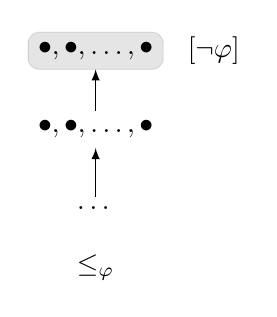
\begin{tikzpicture}
		\node at (0,-0.75){$\le_\phi$};
		\node at (1.5,2){$[\lnot\phi]$};
		\node at (0,2)(0){$\bullet,\bullet,\dots,\bullet$};
		\node at (0,1)(1){$\bullet,\bullet,\dots,\bullet$};
		\node at (0,0)(2){\dots};
		\path[-latex] (2) edge (1)(1) edge (0);
		\fill[draw, opacity=0.1, rounded corners=4]
			(0.south)--
			(0.south west)--
			(0.west)--
			(0.north west)--
			(0.north)--
			(0.north east)--
			(0.east)--
			(0.south east)--
			(0.south);
	\end{tikzpicture}
	\caption{
		A schematic depiction of a total preorder $\le_{\phi}$ 
		in an e-faithful assignment.
		As usual, bullets stand for interpretations.
		Models of $\lnot\phi$ (i.e., interpretations not satisfying $\phi$)
		are shaded in gray. 
	}
	\label{fig:3-enforcement-efaithful-schematic}
\end{figure}

To fix notation, an $\L$-assignment $\as$ on interpretations
is \emph{e-faithful} if it satisfies properties $\ooe{5-6}$.
A schematic depiction of a preorder in an e-faithful 
assignment is given in Figure \ref{fig:3-enforcement-efaithful-schematic}.
Note that the models of $\lnot\phi$ are at the very top.


\subsubsection{Enforcement as choice over outcomes}
The next step in modeling enforcement as a choice procedure
is to link up enforcement as an operation on formulas satisfying 
postulates $\ppe{1-6}$ 
to plausibility relations satisfying properties $\ooe{1-6}$.
This is achieved via a choice procedure, 
which in the case of revision and update amounts to picking 
the best outcomes from the models of the newly acquired 
information $\mu$, 
in effect removing models of $\mu$ that are not optimal. 
However, the nature of the enforcement postulates points 
to a choice procedure that is in many ways
different from that of revision and update:
instead of removing models from $\mu$,
an enforcement operator wants to add to the models of $\mu$:
ideally, it adds all the models of $\phi$.
But if this is not 
possible (in case $\phi\lor\mu$ is a tautology),
some models of $\phi$ will have to be discarded.
This is still an optimization-focused behavior, 
but the parameters under which it functions are new:
using a plausibility ranking on interpretations
in this setting 
becomes a question of not which outcomes are 
more readily held on to,
but which are more readily given up:
a small, but, as we will see, important distinction.

To characterize enforcement we introduce a new way 
of choosing based on a total preorder $\le_{\phi}$ on interpretations.
This method uses the preorder $\le_{\phi}$
to incrementally add interpretations to $[\mu]$,
until further addition becomes impossible.
Thus, if $\W$ is a set of interpretations and 
$\le$ is a preorder on interpretations,
then, for $i\geq 1$, the 
\emph{best-to-worst $\le$-level $i$ of $\W$}, denoted $\lvl_\le^i(\W)$,
is defined by taking:
\begin{align*}
\lvl_\le^1(\W) &= \min_\le(\W),\\
\lvl_\le^{i+1}(\W) &= \min_\le(\W\setminus(\lvl^1_{\le}(\W)\cup\dots\cup\lvl_\le^i(\W))).
\end{align*}
The intuition is that the elements on 
level $i$ are the $i^\text{th}$ best elements of $\W$,
according to $\le$:
we intend to construct the set of models of $\phi \en \mu$
iteratively,
by adding interpretations to $\mu$ in successive steps,
and the $\le$-levels of $\W$ will provide the order 
in which to do so.
It is straightforward to see that 
the best-to-worst levels form a partition of the set $\W$.

Next, we must specify how to actually
construct $[\phi \en \mu]$.
If $\W$ is a set of interpretations, 
the \emph{addition operator $\add^i_{\le}(\W)$} is defined,
for $i\ge 1$, as follows:
\begin{align*}
\add_\le^1(\W) &=\W,\\
\add_\le^{i}(\W) &= 
\begin{cases}
\add_\le^{i-1}(\W)\cup\lvl_{\le}^{i-1}(\U\setminus\W),~\text{if}~\add_\le^{i-1}(\W)\cup\lvl_{\le}^{i-1}(\U\setminus\W)\neq\U,\\
\add_\le^{i-1}(\W),~\text{otherwise}.
\end{cases}
\end{align*}

Intuitively, the addition operator starts from $\W$
and iteratively adds interpretations that are not already in $\W$,
in the order prescribed by $\le_\phi$.
Addition of new interpretations is 
controlled by an acceptance condition,
saying that the new result should not be a tautology.
If the acceptance condition is satisfied then the 
interpretations under considerations 
are added and the operator moves on
to the next level; if not, the operator 
falls back to the result obtained at the previous level.
The starting point guarantees that $\W$ 
is included in $\add_\le^{i}(\W)$, for $i\ge 0$.
Note that, since $\W$ is finite and $\le$ is a total preorder, 
this operation also reaches a fixed point,
i.e., there exists an $i\in\mathbb{\W}$ such that
$\add^j_\le(\W)=\add^i_\le(\W)$, for any $j>i$.
Thus, if 
$\W$ is a set of interpretations and $\le$
is a total preorder on $\W$,
then
\emph{the fixed point of the operator $\add$} is denoted by
$\add_\le^\ast(\W)$.

With the notion of the addition operator in hand,
we can now define a choice procedure that exploits 
a total preorder on interpretations to yield 
the result of enforcing $\mu$ with respect to $\phi$.
Thus, if $\as$ is a total, syntax insensitive and e-faithful
assignment, 
the \emph{$\as$-induced $\L$-enforcement operator $\en^\as$} is defined,
for any propositional formulas $\phi $ and $\mu$,
as follows:
$$
[\phi\en^\as\mu]\defeq\add^\ast_{\le_\phi}[\mu].
$$

Conversely, we want to use an $\L$-enforcement operator $\en$
to infer a ranking over interpretations,
under the assumption that choice is made using the iterative approach
described above.
For revision and update, we would do this using the $\L$-proxy 
of a pair of interpretations $w_1$ and $w_2$, 
i.e., a propositional formula $\px_{1,2}$
such that $[\px_{1,2}]=\{w_1,w_2\}$,
to ask the agent which of the two outcomes it 
wants to hold on to.
Enforcement, which, as we have seen, 
is a kind of dual of revision,
requires a different tactic: 
we will use the $\L$-antiproxy
of a pair of interpretations $w_1$ and $w_2$,
i.e., a propositional formula 
$\px_{-1,-2}$ such that $[\px_{-1,-2}]=\U\setminus\{w_1,w_2\}$,
to ask the agent which of the two outcomes it wants to
give up.
Then, 
if $\en$ is an enforcement operator,
the \emph{$\en$-revealed relation $\le_\phi$} is defined by taking,
for any interpretations $w_1$ and $w_2$:
$$
	w_1\le^{\en}_\phi w_2~\text{if}~w_2\notin[\phi\en\px_{-1,-2}].
$$
The rationale here is that $w_2$ is 
less preferred than $w_1$ if it is more readily given up:
since the rules of enforcement say that 
${\px_{-1,-2}}\subseteq [\phi\en \px_{-1,-2}]\subset\U$,
interpretations $w_1$ and $w_2$ cannot both 
be added to $\phi \en \px_{-1,-2}$
so a choice must be as to which to give up.
If $w_2$, rather than $w_1$, is given up, this indicates that
$w_1$ is preferred to $w_2$; giving both of them up means that
they are equally preferred. 

\begin{figure}\centering
	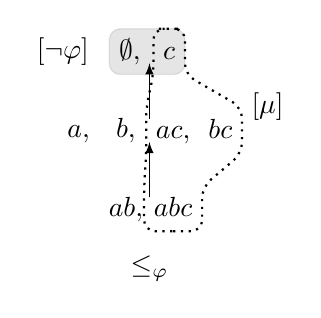
\begin{tikzpicture}
		\node at (0,-0.75){$\le_\phi$};

		\node at (-0.3,0)(ab){$ab,$};
		\node at (0.3,0)(abc){$abc\vphantom{,}$};
		\node[inner sep=0.4em] at (0,0)(a1){};
	
		\node at (-0.9,1)(a){$\vphantom{b,}a,$};	
		\node at (-0.3,1)(b){$b,$};		
		\node at (0.3,1)(ac){$\vphantom{\emptyset}ac,$};
		\node at (0.9,1)(bc){$bc\vphantom{\emptyset,}$};
		\node[inner sep=0.4em] at (0,1)(a2){};

		\node at (-0.25,2)(e){$\emptyset,$};
		\node at (0.25,2)(c){$\vphantom{\emptyset,}c$};
		\node[inner sep=0.4em] at (0,2)(a3){};

		\node at (-1.1,2){$\mods{\lnot\phi}$};
		\node at (1.5,1.3){$[\mu]$};
	
		\path[-latex] (a1) edge (a2)(a2)edge(a3);
		
		\fill[draw, opacity=0.1, rounded corners=4]
			(c.south)--
			(e.south)--
			(e.south west)--
			(e.west)--
			(e.north west)--
			(e.north)--
			(c.north)--
			(c.north east)--
			(c.east)--
			(c.south east)--
			(c.south);
		\draw[thick, dotted, rounded corners=4]
			(abc.south)--
			(abc.south east)--
			(abc.east)--
			(abc.north east)--
			(bc.south east)--
			(bc.east)--
			(bc.north east)--
			(c.south east)--
			(c.east)--
			(c.north east)--
			(c.north)--
			(c.north west)--
			(c.west)--
			(c.south west)--
			(ac.north west)--
			(ac.west)--
			(ac.south west)--
			(abc.north west)--
			(abc.west)--
			(abc.south west)--
			(abc.south);
	\end{tikzpicture}
	\caption{
		A total preorder $\le_{\phi}$ assigned to $\phi$,
		with $[\phi]=\{a,b,ab,ac,bc,abc\}$,
		by a total, syntax insensitive and e-faithful 
		assignment.
		Note that the interpretations not satisfying $\phi$,
		i.e., models of $[\lnot\phi]$,
		are the least preferred outcomes in this preorder
		and are in the gray region.
		The new information is $\mu$,
		with $[\mu]=\{c,ac,bc,abc\}$.
		Enforcing $\mu$ with respect to $\phi$ involves adding 
		interpretations to $[\mu]$ that are not already in 
		$[\mu]$ in the order prescribed by $\le_{\phi}$,
		unless a tautology is created.
	}
	\label{fig:3-enforcement-preorder-operator-interaction}
\end{figure}	

\begin{xmpl}{The art of diagnosis, using a preorder on outcomes}{3-enforcement-preorder-operator-interaction}
	For the setting in Example \ref{ex:3-enforcement-basic-setup},
	with $\phi=a\lor b$ and $\mu=c$, 
	we have that $[\phi]=\{a,b,ab,ac,bc,abc\}$ and $[\mu]=\{c,ac,bc,abc\}$.
	Consider, first, a total, syntax independent $\L$-assignment $\as$ on interpretations
	that assigns to $\phi$ the preorder $\le_{\phi}$
	in Figure \ref{ex:3-enforcement-preorder-operator-interaction}.
	We obtain $[\phi \en \mu]$ by applying the addition operator $\add$
	to $[\mu]$.
	The addition operator starts from $[\mu]$ 
	and takes the levels of ${\lnot\mu}$ in order, trying to add them
	to $\mu$ while avoiding the creation of a tautology. 
	The operation is successful for the first and second levels, after which
	a fixed point is reached.
	The result is:
	\begin{align*}
		[\phi\en\mu] &=\add^\ast_{\le_\phi}[\mu]\\
					 &=([\mu]\cup\{ab\})\cup \{a,b\}\\
					 &=\{a,b,c,ab,ac,bc,abc\}.
	\end{align*}
	Converting the result back into a propositional formula,
	we obtain that $\phi\en\mu\equiv a\lor b\lor c$.

	Conversely, the ranking between two outcomes, 
	say $a$ and $ab$, 
	relative 
	to the prior information $\phi$, with $[\phi]=\{a,b,ab,ac,bc,abc\}$,
	can be elicited by asking the agent 
	to enforce the new information $\px_{-1,-2}$,
	with $[\px_{-1,-2}]=\{\emptyset,b,c,ac,bc,abc\}$.
	Supposing the result is $[\phi\en\px_{-1,-2}]=[\px_{-1,-2}]\cup\{ab\}$,
	we can conclude that, according to the $\en$-revealed ranking,
	it holds that $ab<^{\en}_{\phi}a$.
	This is consistent with $\le_{\phi}$ 
	as depicted in Figure \ref{fig:3-enforcement-preorder-operator-interaction}.
\end{xmpl}

The test of our construction, of course, is whether 
postulates $\ppe{1-6}$, properties $\ooe{1-6}$ and the choice 
procedure formalized by the addition operator $\add$
work together to describe a single belief change mechanism.
The validation comes in the form of a representation theorem,
which shows that these notions cohere with each other.
Before introducing the result, though,
we need to explain what it means for an $\L$-assignment 
$\as$ on interpretations to represent an enforcement operator.
Thus, if $\en$ is an $\L$-enforcement operator 
and $\as$ is an $\L$-assignment on interpretations,
then \emph{$\as$ represents $\en$}
(alternatively, \emph{$\en$ is represented by $\as$})
if, for any propositional formulas $\phi$ and $\mu$,
it holds that $[\phi\en\mu]=\add^\ast_{\le_\phi}[\mu].$
We can now introduce the main representation theorem 
of this section.

\begin{thm}{}{3-enforcement-repr}
	An $\L$-enforcement operator $\en$ 
	satisfies postulates $\ppe{1-6}$ if and only if
	there exists an $\L$-assignment $\as$
	that satisfies properties $\ooe{1-6}$
	(i.e., that is total, syntax insensitive and
	e-faithful)
	and that represents the operator $\en$.
\end{thm}
\begin{prf*}{}{}%
	(``$\Leftarrow$'')
	Note that a preorder $\le_{\phi}$ that satisfies properties 
	$\ooe{1-6}$ can be seen as a preorder $\le_{\lnot\phi}$,
	i.e., a preorder depending on $\lnot\phi$, 
	by taking $w_1\le_{\lnot\phi}w_2$ if $w_2 \le_{\phi}w_1$,
	i.e., by turning $\le_{\phi}$ upside down.
	In this case, $\le_{\lnot\phi}$ satisfies 
	the revision properties $\oor{1-7}$.
	Note that in this setting we have that the complement of 
	$\add^\ast_{\le_\phi}[\mu]$ consists of the minimal 
	models of $\lnot\mu$ in the preorder $\lnot\phi$ as just 
	defined. We can now see that the upside down assignment 
	corresponds to a total, syntax insensitive r-faithful assignment,
	which corresponds to a revision operator $\re$ that 
	satisfies postulates $\ppr{1-6}$.
	Furthermore, we get that 
	$[\phi\en\mu]=\U\setminus(\lnot\phi\re\lnot\mu)$,
	which, by Proposition \ref{prop:3-enforcement-duality},
	implies that $\en$ satisfies postulates $\ppe{1-6}$.

	(``$\Rightarrow$'')
	The $\en$-revealed assignment is the assignment we are looking for,
	and it is straightforward to check that it satisfies properties $\ooe{1-6}$
	and that it represents the operator $\en$.
\end{prf*}

A quick note is in order on previous results.
Existing work on propositional enforcement \cite{HaretWW18} 
has used partial orders 
on sets of interpretations (or, alternatively, on formulas)
to represent enforcement operators, 
but a nice representation in terms of preorders on interpretations themselves, 
\`a la Theorem \ref{thm:3-revision-repr-km-total}, was left open.
Here we filled this gap.
Note, also, that a representation in terms of preorder on interpretations
can be obtained in a more naive way, by using 
Equations \ref{eq:revision-to-enforcement} 
and \ref{eq:enforcement-to-revision} 
and Theorem \ref{thm:3-revision-repr-total}.
Thus, given an enforcement operator $\en$ 
satisfying postulates $\ppe{1-6}$, 
we can immediately infer that there exists 
an $\L$-assignment $\as$ on interpretations
that satisfies properties $\oor{1-5}$ and $\oor{7}$ 
such that, for any propositional formulas $\phi$ and $\mu$, 
the following holds:
$$
	[\phi\en\mu] = [\lnot(\lnot\phi\re^\en\lnot\mu)]=\U\setminus\min_{\le_{\lnot\phi}}[\lnot\mu].
$$
In other words, we can use an assignment representing 
the $\en$-induced $\L$-revision operator $\re^\en$ to represent $\en$.
However, this expression is not very informative and, 
as we have shown, unnecessarily circuitous.

\subsubsection{Distance-based enforcement operators}
Theorem \ref{thm:3-enforcement-repr} offers some insight 
into how to construct concrete enforcement operators:
find a way to generate e-faithful assignments, 
i.e., preorders on interpretations in which the top elements 
are the non-models of $\phi$.
It turns out that the tried and tested methods of 
quasi-distances between interpretations
and aggregation functions 
used in revision and update work here as well, with minimal adjustment.

We bring up aggregation functions only to settle straight away 
that the only aggregation function we will use in this section 
is the $\min$ aggregation function: we will be using it, however,
in a slightly different way than in revision.
For the next definition, recall that the size of the set $\Atoms$
is assumed to be $m$.
If $\dd$ is a quasi-distance between interpretations,
$\phi$ is a propositional formula and $w$ is an interpretation,
then the 
\emph{$(\dd,\:m-\min)$-induced distance $\dd^{m-\min}(\phi,w)$ between $\phi$ and $w$} 
is defined as:
$$
	\dd^{m-\min}(\phi,w) = m-\min(\dd(v,w))_{v\in[\phi]}.
$$
Intuitively, $\dd^{m-\min}(\phi,w)$ can be thought of as the inverse
of the more familiar notion $\dd^{\min}(\phi,w)$ 
(see Sections \ref{sec:2-distances} or \ref{sec:3-revision}):
a penalty is introduced for $w$ the closer it is to the models of $\phi$,
such that the interpretations closest to $\phi$ end up receiving the 
highest score
and the interpretations furthest to $\phi$ receive the lowest score,
i.e., $\phi$ is such that it is better to be far away from it than close to it.

Following up, the \emph{$(\dd,\:m-\min)$-induced ranking $\le^{\dd,\:m-\min}_{\phi}$}
is defined as:
$$
	w_1\le^{\dd,\:m-\min}_\phi w_2~\text{if}~\dd^{m-\min}(\lnot\phi,w_1)\le\dd^{m-\min}(\lnot\phi,w_2).
$$
What we are saying, in effect, is that $w_1$ is preferred to $w_2$ relative to $\phi$,
according to $\le^{\dd,\:m-\min}_{\phi}$ if $w_1$ is farther away from $\lnot\phi$ than $w_2$.
If $\dd$ is a quasi-distance,
the \emph{${(\dd,\:m-\min)}$-induced assignment $\as^{\dd,\:m-\min}$} is obtained by taking 
$\as^{\dd,\:m-\min}\!\!(\phi)=\le_\phi^{\dd,\:m-\min}$,
for any propositional formula $\phi$.
In the same vein, the \emph{${(\dd,\:m-\min)}$-induced $\L$-enforcement operator $\en^{\dd,\:m-\min}$} 
is the operator induced by the assignment $\as^{\dd,\:m-\min}$.
This allows us to generate total, syntax insensitive e-faithful assignments.

\begin{prp}{}{3-enforcement-d-induced-preorder}
	If $\dd$ is a quasi-distance between interpretations and $\phi$ is a propositional formula, 
	the ${(\dd,\:m-\min)}$-induced ranking $\le^{\dd,\:m-\min}_\phi$ 
	satisfies properties $\ooe{1-6}$, 
	i.e., $\le^{\dd,\:m-\min}_\phi$ is a total preorder 
	on interpretations that	is syntax insensitive and 
	makes the models of $\lnot\phi$ the 
	$\le^{\dd,\:m-\min}_\phi$-maximal elements.
\end{prp}
\begin{prf*}{}{}%
	It is straightforward to see that $\le_{\phi}^{\dd,\:m-\min}$ 
	is a total preorder on interpretations,
	i.e., that $\le_{\phi}^{\dd,\:\min}$ satisfies properties $\ooe{1-3}$.
	Since the definition of $\le_{\phi}^{\dd,\:m-\min}$ 
	depends only on the interpretations,
	$\le_{\phi}^{\dd,\:m-\min}$ also satisfies property $\ooe{4}$.
	Finally, it holds that:
	$\dd^{m-\min}(\lnot\phi,w) = m- \min(\dd(v,w))_{v\in[\lnot\phi]} = m$ if and only if
	$w\in[\lnot\phi]$, 
	which implies that models of $\lnot\phi$ are the $\le_{\phi}^{\dd,\:m-\min}$-maximal
	elements in $\le_{\phi}^{\dd,\:m-\min}$,
	i.e., $\le_{\phi}^{\dd,\:m-\min}$ satisfies 
	properties $\ooe{5}$ and $\ooe{6}$, 
	for any propositional formula $\phi$.		
\end{prf*}

Proposition \ref{prop:3-enforcement-d-induced-preorder} 
implies that the $({\dd,\:m-\min})$-induced assignment $\as^{\dd,\:m-\min}$ 
is total, e-faithful and syntax insensitive, 
which, by Theorem \ref{thm:3-enforcement-repr}, 
implies that the $({\dd,\:m-\min})$-induced $\L$-enforcement operator 
$\en^{\dd,\:\min}$ satisfies postulates $\ppe{1-6}$.

\begin{crl}{}{3-enforcement-d-induced-operator}
	If $\dd$ is a quasi-distance between interpretations, 
	the $(\dd,\:m-\min)$-induced $\L$-enforcement 
	operator $\en^{\dd,\:m-\min}$ 
	satisfies postulates $\ppe{1-6}$.
\end{crl}

As examples of concrete distances we can use the Hamming distance $\dd_{\hamming}$
and the drastic distance $\dd_{\drastic}$, giving rise to the $\L$-enforcement operators 
$\en^{\hamming,\:m-\min}$ and $\en^{\drastic,\:m-\min}$.

\begin{figure}\centering
	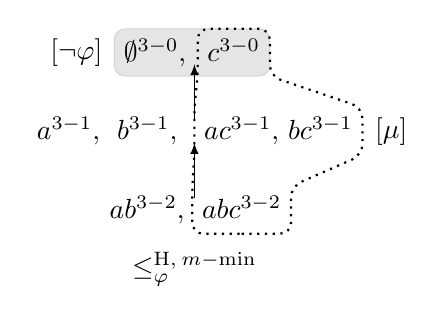
\begin{tikzpicture}
		\node at (0,-0.75){$\le^{\hamming,\:m-\min}_\phi$};

		\node at (-0.6,0)(ab){$ab^{3-2},$};
		\node at (0.6,0)(abc){$abc^{3-2}\vphantom{,}$};
		\node[inner sep=0.4em] at (0,0)(a1){};
	
		\node at (-1.6,1)(a){$\vphantom{b,}a^{3-1},$};	
		\node at (-0.6,1)(b){$b^{3-1},$};		
		\node at (0.6,1)(ac){$\vphantom{\emptyset}ac^{3-1},$};
		\node at (1.6,1)(bc){$bc^{3-1}\vphantom{\emptyset,}$};
		\node[inner sep=0.4em] at (0,1)(a2){};

		\node at (-0.5,2)(e){$\emptyset^{3-0},$};
		\node at (0.5,2)(c){$\vphantom{\emptyset,}c^{3-0}$};
		\node[inner sep=0.4em] at (0,2)(a3){};

		\node at (-1.5,2){$\mods{\lnot\phi}$};
		\node at (2.5,1){$[\mu]$};
	
		\path[-latex] (a1) edge (a2)(a2)edge(a3);
		
		\fill[draw, opacity=0.1, rounded corners=4]
			(c.south)--
			(e.south)--
			(e.south west)--
			(e.west)--
			(e.north west)--
			(e.north)--
			(c.north)--
			(c.north east)--
			(c.east)--
			(c.south east)--
			(c.south);
		\draw[thick, dotted, rounded corners=4]
			(abc.south)--
			(abc.south east)--
			(abc.east)--
			(abc.north east)--
			(bc.south east)--
			(bc.east)--
			(bc.north east)--
			(c.south east)--
			(c.east)--
			(c.north east)--
			(c.north)--
			(c.north west)--
			(c.west)--
			(c.south west)--
			(ac.north west)--
			(ac.west)--
			(ac.south west)--
			(abc.north west)--
			(abc.west)--
			(abc.south west)--
			(abc.south);
	\end{tikzpicture}
	\caption{
		The preorder $\le^{\hamming,\:m-\min}_{\phi}$ 
		assigned to $\phi$,
		with $[\phi]=\{a,b,ab,ac,bc,abc\}$,
		by the $\as^{\hamming,\:m-\min}$ 
		assignment.
		The superscripts denote the distance to $\lnot\phi$
		subtracted from the number of atoms in $\Atoms$,
		which in this case is $3$.
		Note that the interpretations not satisfying $\phi$,
		i.e., models of $[\lnot\phi]$,
		get a score of $3$,
		which makes them the least 
		preferred outcomes.
	}
	\label{fig:3-enforcement-hamming-op}
\end{figure}	

\begin{xmpl}{The art of diagnosis, using distances}{3-enforcement-hamming-op}
	For the setting in Example \ref{ex:3-enforcement-basic-setup},
	with 
	$\Atoms=\{a,b,c\}$,
	$\phi=a\lor b$ and $\mu=c$, 
	the $\L$-assignment $\as^{\hamming,\:m-\min}$ 
	generates the preorder $\le^{\hamming,\:m-\min}_{\phi}$  
	in Figure \ref{fig:3-enforcement-hamming-op}.
	Note that $\le^{\hamming,\:m-\min}_{\phi}$ is the same
	as the preorder $\le_{\phi}$ in Figure \ref{fig:3-enforcement-preorder-operator-interaction}.
	We obtain, as before, that $[\phi\en\mu]=\add^{\ast}_{\le_{\phi}}[\mu]=\{a,b,c,ab,ac,bc,abc\}$.
\end{xmpl}























\section{Merging}\label{sec:3-merging}
If agents deliberate with respect 
to a small number of independent alternatives, 
as is the case in a typical election, 
aggregation of different viewpoints 
is well understood due to existing research 
in the field of social choice \cite{Zwicker16,BaumeisterR16}.
But if agents have to decide on multiple 
interconnected issues at the same time,
then the number of possible alternatives 
can grow too large to expect agents 
to have explicit preferences over the whole set.
We have encountered this kind of scenario 
in Example \ref{ex:1-merging-motivation},
where we have been introduced to four 
Academy members trying to decide who will 
be the nominees in this year's \emph{Best Director} category.

\begin{xmpl}{$\#$OscarsSoFossilized}{3-merging-basic-setup}
	In Example \ref{ex:1-merging-motivation}
	the names being circulated are Alma Har'el, Bong Joon Ho and C\'eline Sciamma,
	represented by propositional variables
	$a$, $b$ and $c$, respectively.
	The decision as to who will be the nominees
	is left up to four Academy members.
	Each of the four members has their own opinion 
	about who should be nominated, represented by propositional formulas 
	$\phi_1 = a\land b$,
	$\phi_2 = a\land (b\lor c)$,
	$\phi_3 = \lnot a\land b \land \lnot c$.
	and
	$\phi_4 = \lnot a \land\lnot b\land c$.
	The final lineup should consist of only two people,
	i.e., the individual opinions should be aggregated subject to the constraint
	$\mu=(a\land b\land \lnot c)\lor (a\land\lnot b\land c)\lor(\lnot a\land b\land c)$.
	These opinions are collectively inconsistent, 
	but none of them weighs more than the others.
\end{xmpl}

In Example \ref{ex:3-merging-basic-setup},
a standard social choice procedure would require
the Academy members to provide a ranking 
of all the possible lists of two nominees, 
or, as we code them here, of the outcomes 
$ab$, $bc$, $ac$.
Though this would not be too difficult for this example,
the cognitive burden on the agents will certainly become too big
if the number of possibilities or the size of the lineup 
grew even slightly. 
This is certain to be the case even for the Oscars:
Example \ref{ex:3-merging-basic-setup} is only a toy example,
since the real world list of \emph{Best Director} nominees is 
usually made up of five people, and the list of possible 
nominees is much larger. 
In the real world scenario, asking Academy members to rank all possible
combinations of five directors is clearly unfeasible.

This problem, known more generally as \emph{combinatorial voting} \cite{LangX16}, 
acquires a knowledge representation dimension 
as agents need compact ways to express their positions over 
a large domain, and automatizable procedures 
to perform reasoning with such positions.
Merging, in this context, can prove useful,
as it provides a versatile framework in which different agents 
can combine their positions on a fixed set of issues,
expressed as propositional formulas,
into a collective perspective, expressed, likewise,
as a propositional formula \cite{KoniecznyP02,KoniecznyP11}.

In Example \ref{ex:3-merging-basic-setup}
a merging operator should combine the information 
provided by the four Academy members
while making sure that the cardinality constraint $\mu$ is satisfied.
What the theory of belief merging offers is
a core set of postulates to assess the rationality of any merging operator,
and a range of concrete operators tailored according to these principles.
Seeing merging operators as a type of collective decision procedure
is a natural interpretation of the process:
the propositional atoms in the alphabet can be taken 
to encode issues that are deliberated upon,
while truth-value assignments to atoms, 
i.e., the interpretations or outcomes, 
encode combinations of issues that could make it 
into the final result, and over which agents can have preferences.
The propositional formulas submitted by agents 
represent the way in which issues are interconnected in the agents' preferences,
and the result is a set of ``winning'' interpretations,
representable as a propositional formula, 
that respect the integrity constraint of the merging process. 

\subsubsection{Postulates}
An \emph{$\L^{n}$-merging operator $\me$} 
is a function $\me\colon\L^n\rightarrow\L$,
taking as input 
a propositional profile $\P=(\phi_i)_{1\le i \le n}$
and a propositional formula $\mu$,
and returning a propositional formula, 
denoted by $\me_\mu(\P)$.
In the context of merging the formula $\mu$,
which we normally call the new information,
is called an \emph{integrity constraint}.
Merging is a multi-agent operation,
in the sense that the formulas in a profile $\P$
originate with different agents, 
usually gathered in the set $N=\{1,\dots,n\}$,
with formula $\phi_{i}$ corresponding to agent $i$.

The following postulates are typically taken to provide a core set of rationality constraints
any merging operator $\me$ is expected to satisfy.
They are expected to hold for any propositional profiles $\P$, $\P_1$, $\P_2$,
formulas $\phi_1$, $\phi_2$
and constraints $\mu$, $\mu_{1}$ and $\mu_{2}$:

\begin{description}
	\item[($\ppm{0}$)] $\me_\mu(\P)\models\mu$.
	\item[($\ppm{1}$)] If $\mu$ is consistent, then $\me_\mu(\P)$ is consistent.
	\item[($\ppm{2}$)] If $\bigwedge\P\land\mu$ is consistent, then $\me_\mu(\P)\equiv\bigwedge\P\land\mu$.
	\item[($\ppm{3}$)] If $\P_1\equiv \P_2$ and $\mu_1\equiv\mu_2$, 
	then $\me_{\mu_1}(\P_1)\equiv\me_{\mu_1}(\P_2)$.
	\item[($\ppm{4}$)] If $\phi_1\models\mu$ and $\phi_2\models\mu$, 
	then $\me_\mu(\phi_1,\phi_2)\land\phi_1$ is 
	consistent if and only if $\me_\mu(\phi_1,\phi_2)\land\phi_2$ is consistent.
	\item[($\ppm{5}$)] $\me_\mu(\P_1)\land\me_\mu(\P_2)\models\me_\mu(\append{\P_1}{\P_2})$.
	\item[($\ppm{6}$)] If $\me_\mu(\P_1)\land\me_\mu(\P_2)$ is consistent, then 
	$\me_\mu(\append{\P_1}{\P_2})\models\me_\mu(\P_1)\land\me_\mu(\P_2)$.
	\item[($\ppm{7}$)] $\me_{\mu_1}(\P)\land\mu_2\models\me_{\mu_1\land\mu_2}(\P)$.
	\item[($\ppm{8}$)] If $\me_{\mu_1}(\P)\land\mu_2$ is consistent, then
	$\me_{\mu_1\land\mu_2}(\P)\models\me_{\mu_1}(\P)\land\mu_2$.
\end{description}

Postulate $\ppm{0}$ says that the merging result $\me_{\mu}(\P)$ should
satisfy the constraint $\mu$.
Postulate $\ppm{1}$ says that the result 
should be consistent if $\mu$ is consistent.
Postulate $\ppm{2}$ requires that if there 
is any agreement between the formulas in $\P$ and $\mu$,
then the merged result is nothing more than the agreed upon outcomes.
Postulate $\ppm{3}$ says that the result 
should be insensitive to the syntax of the formulas involved.
Postulate $\ppm{4}$ stipulates that merging two formulas $\phi_1$ and $\phi_2$ should be fair,
in the sense that if the result contains outcomes consistent with one of the formulas, it should contain 
results consistent with the other as well.
Postulates $\ppm{5-6}$ say that the result should
include outcomes that are unanimously accepted across subprofiles.
Postulates $\ppm{7-8}$ say that the result 
and coherent when varying the constraint.

Though postulates $\ppm{0-8}$ are referred to here using our custom naming convention,
in the literature they are more commonly known as the $IC$-postulates \cite{KoniecznyP02,KoniecznyP11},
where `$IC$' stands for \emph{integrity constraint} and indicates that merging is done within the purview of 
the condition $\mu$, which must be satisfied by the merging result $\me_\mu(\P)$.

Note that, insofar as a profile $\P=(\phi_i)_{1\le i \le n}$ 
is identified with the single propositional 
formula $\bigwedge_{\phi_i\in\P}\phi_{i}$, 
then postulates $\ppm{0-3}$ and $\ppm{7-8}$ correspond to revision postulates
$\ppr{1-4}$ and $\ppr{5-6}$, respectively,
where $\bigwedge\P$ is the prior belief and $\mu$ is the newly acquired information.
Thus, another way of looking at a merging operator $\me$ 
is to see it as a revision operator that needs to satisfy some additional
properties, besides the standard ones presented in Section \ref{sec:3-revision}.
These properties are postulates $\ppm{4-6}$, and what they add 
is the notion that the formulas that go into the prior belief (or rather, their models)
should carry equal weight in the change process. 
This corresponds to the idea that merging is a public, 
or social operation, whose participants should be treated fairly.
Consequently, postulates $\ppm{0-8}$ are best understood as axiomatizing a decision procedure 
based on the aggregation of information coming from different sources, i.e., the formulas in $\P$.

\begin{xmpl}{Possible Oscar nominees}{3-merging-postulates}
	For the merging scenario in Example \ref{ex:3-merging-basic-setup}
	the profile is $\P=(\phi_1,\phi_2,\phi_3,\phi_4)$,
	where 
	$\phi_1 = a\land b$,
	$\phi_2 = a\land (b\lor c)$,
	$\phi_3 = \lnot a\land b \land \lnot c$
	and
	$\phi_4 = \lnot a \land\lnot b\land c$.
	Examples \ref{ex:1-merging-motivation} 
	and \ref{ex:3-merging-basic-setup} provide the meaning
	for these formulas.
	The constraint is represented by the propositional formula
	$\mu=(a\land b\land \lnot c)\lor (a\land\lnot b\land c)\lor(\lnot a\land b\land c)$,
	with $[\mu]=\{ab,bc,ac\}$.


	Suppose that $\me$ is a merging operator that satisfies postulates $\ppm{0-8}$
	and $\me_\mu(\P)\equiv (a\land b)\lor(b\land c)$,
	i.e., $[\me_\mu(\P)]=\{ab,bc\}$. This result is in line with 
	postulate $\ppm{1}$ (i.e., it is consistent)
	and	with postulate $\ppm{0}$ (i.e., implies $\mu$).
	The models of $[\me_\mu(\P)]$ encode the makeup of the list of nominees,
	e.g., $ab$ means that Alma Har'el and Bong Joon Ho (but not C\'eline Sciamma) will be nominated.
\end{xmpl}

As with revision and the other belief change operations we 
have looked at in this chapter, 
the positions of the agents could be beliefs, intentions or simply 
combinations of issues that agents find desirable, 
and would like to see in the result.
The consistent insistence on insensitivity to syntax means that 
the propositional formulas that stand for the agents' positions 
are, in a sense, just window dressing for their models.
This is another way of saying that
belief change operations are interested more in the underlying issues 
rather than in how they are expressed.
Of course, the representation may matter for cognitive or computational 
purposes, but for the belief change operators we consider here 
the formulas are just compact representations of sets of outcomes the agents 
are interested in.
Thus, whether or not the formulas encode (actual) beliefs is not of 
immediate crucial importance to a merging operator:
postulates $\ppm{0-8}$ are neutral with respect to the cognitive attitude
being expressed.

That being said, the exact meaning of the formulas \emph{will} matter 
if we want to be more specific about the type of information aggregation a belief merging 
operator performs. Thus, there is a significant difference between aggregating 
bits of information the agents believe are true, when there is, actually,
a true state of the world,
versus aggregating sets of issues the agent want to see obtain,
in which case there might not be a true answer at all.
In the former case the purpose of a merging operator is to track the truth,
whereas in the latter case the purpose of a merging operator is to be fair 
towards the participants.
Correspondingly, the criteria a merging operator is expected to satisfy 
will be different depending on the kind of task it is used for:
a truth-tracking operator will be expected to be accurate, 
whereas a fair merging operator will be expected to be impartial 
towards the agents, strategyproof or proportional.

In this work we are interested in merging more as a tool for collective decision 
making than as a way of aggregating information about the world, 
and will therefore focus on the fairness aspects of merging.
Work on the truth-tracking abilities of merging exists \cite{EveraereKM10},
but is outside the scope of the current work.


\subsubsection{Preferences over outcomes}
In the context of merging, 
preference orders are ushered in 
through an \emph{$\L^{n}$-assignment $\as$ on interpretations}, 
which is a function $\as\colon\L^n\rightarrow 2^{\U\times\U}$ 
that maps $\L$-profiles
to preference orders on interpretations.
In Sections \ref{sec:3-revision} and \ref{sec:3-update}
we have modeled both total and partial preorders,
but here we will work mainly with total preorders.
Since we want to pursue the parallel between 
merging and a collective decision process,
the relation $\le_{\P}$ assigned to a profile 
$\P=(\phi_i)_{1\le i \le n}$
by an $\L^n$-assignment $\as$ on interpretations
can be thought of as the collective ranking, 
obtained by aggregating the preferences of each agent 
in $N=\{1,\dots,n\}$.
In this context, the preferences of the agents themselves 
are given by $\le_{(\phi_{i})}$,
i.e., by the preference associated with the profile $(\phi_{i})$ 
having only $\phi_{i}$ as element.
In the interest of readability, we will generally write 
simply $\le_{\phi_i}$ instead of $\le_{(\phi_i)}$, 
when only one agent is involves.

Under the assumption of an $\L^n$-assignment $\as$ on interpretations,
we have both that the individual preference orders $\le_{\phi_{i}}$, for $i\in N$,
as well as the collective preference $\le_{\P}$, exist.
The purpose of merging, however, is to make sure 
not only that the individual and collective preference 
orders exist, but that they also have desirable properties,
i.e., that the collective preference order can be seen 
to aggregate, in a fair and reasonable way,
the information provided by the individual preference orders.
This is ensured by writing down desirable properties 
of an $\L^n$-assignment $\as$ on interpretations.
The properties an $\L^n$-assignment is expected to satisfy 
include some familiar properties, but also some new ones.
Recall that two propositional profiles $\P_1$ and $\P_2$
are equivalent, written $\P_1\equiv\P_2$, if there is a bijection
$f\colon\P_1\rightarrow\P_2$ such that $f(\phi_i)\equiv \phi_i$,
for any $\phi_i\in\P_1$.
The properties are expected to apply for any propositional profiles 
$\P$, $\P_1$, $\P_2$, propositional formulas $\phi_1$ and $\phi_2$,
and interpretations $w$, $w_1$ and $w_2$:

\begin{description}
	\item[($\oom{1}$)] $w\le_\P w$.
	\item[($\oom{2}$)] If $w_1\le_\P w_2$ and $w_2\le_\P w_3$, then $w_1\le_\P w_3$.
	\item[($\oom{3}$)] $w_1\le_\P w_2$ or $w_2\le_\P w_1$.
	\item[($\oom{4}$)] If $\P_1\equiv\P_2$, then $\le_{\P_1} = \le_{\P_2}$.		
	\item[($\oom{5}$)] If $w_1,w_2\in[\P]$, then $w_1\approx_\P w_2$.
	\item[($\oom{6}$)] If $w_1\in [\P]$ and $w_2\notin [\P]$, then $w_1 <_{\P} w_2$.
	\item[($\oom{7}$)] If $\phi_1$ and $\phi_2$ are consistent and $w_1\in[\phi]$,
		then there exists $w_2\in[\phi_2]$ such that $w_2\le_{(\phi_1,\phi_2)}w_1$. 
	\item[($\oom{8}$)] If $w_1\le_{\P_1} w_2$ and $w_1\le_{\P_2} w_2$, 
		then $w_1\le_{\append{\P_1}{\P_2}} w_2$.
	\item[($\oom{9}$)] If $w_1\le_{\P_1} w_2$ and $w_1<_{\P_2} w_2$, 
		then $w_1<_{\append{\P_1}{\P_2}} w_2$.
\end{description}

Properties $\oom{1-3}$ imply that $\le_{\P}$ is a total preorder on interpretations,
and are identical to revision properties $\oor{1-3}$.
Property $\oom{4}$ expresses syntax insensitivity in the context of merging.
Properties $\oom{5-6}$ say that models of a profile $\P$ are the 
uniquely minimal elements in $\le_{\P}$, 
and are equivalent to revision properties $\oor{5}$ and $\oor{7}$, respectively.
Property $\oom{7}$ says that models of two formulas $\phi_{1}$ and $\phi_{2}$
should be treated equally when merging $\phi_{1}$ and $\phi_{2}$,
in the sense that it should not be the case that some model of $\phi_{1}$
gets chosen while all models of $\phi_{2}$ are left out 
(assuming it is possible to choose models from both $\phi_{1}$ and $\phi_{2}$).
Property $\oom{8}$ says that if $w_{1}$ is considered at least as good as $w_{2}$
according to both profiles $\P_{1}$ and $\P_{2}$, then 
$w_{1}$ is also considered at least as good as $w_{2}$ according to the 
profile $\P_{1}+ \P_{2}$, obtained by concatenating $\P_{1}$ and $\P_{2}$;
in other words, agreement about $w_{1}$ and $w_{2}$ carries over to the 
aggregated result.
Property $\oom{9}$ says that if 
if $w_{1}$ is considered at least as good as $w_{2}$
according to both profiles $\P_{1}$ and $\P_{2}$
and, in addition, 
$w_{1}$ is considered strictly better than $w_{2}$
according to at least one of the profiles $\P_{1}$ and $\P_{2}$,
then $w_{1}$ is considered strictly better than $w_{2}$
according to the 
profile $\P_{1}+ \P_{2}$, obtained by concatenating $\P_{1}$ and $\P_{2}$.

\begin{figure}\centering
	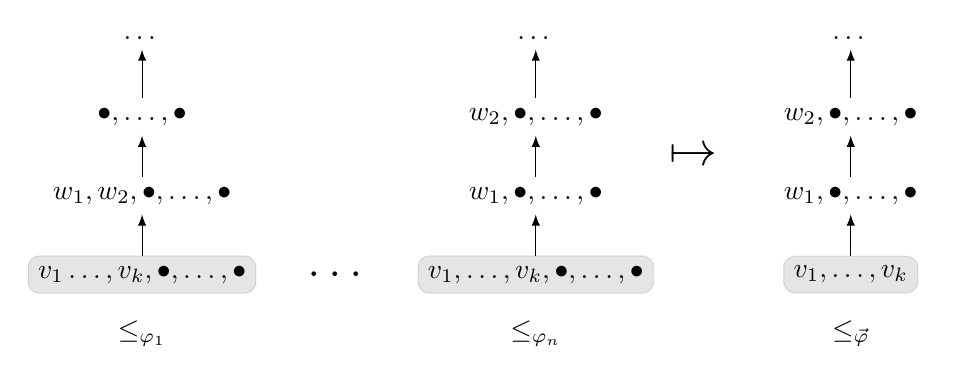
\begin{tikzpicture}
		\node at (0,-0.75){$\le_{\phi_{1}}$};
		\node at (0,0)(0){$v_{1}\dots,v_{k},\bullet,\dots,\bullet$};
		\node at (0,1)(1){$w_1,w_2,\bullet,\dots,\bullet$};
		\node at (0,2)(2){$\bullet,\dots,\bullet$};
		\node at (0,3)(3){\dots};
		\path[-latex] (0) edge (1)(1) edge (2)(2)edge(3);
		\fill[draw, opacity=0.1, rounded corners=4]
			(0.south)--
			(0.south west)--
			(0.west)--
			(0.north west)--
			(0.north)--
			(0.north east)--
			(0.east)--
			(0.south east)--
			(0.south);

		\node at (2.5,0){\LARGE $\dots$};
	
		\node at (5,-0.75){$\le_{\phi_{n}}$};
		\node at (5,0)(0){$v_{1},\dots,v_{k},\bullet,\dots,\bullet$};
		\node at (5,1)(1){$w_1,\bullet,\dots,\bullet$};
		\node at (5,2)(2){$w_2,\bullet,\dots,\bullet$};
		\node at (5,3)(3){\dots};
		\path[-latex] (0) edge (1)(1) edge (2)(2)edge(3);
		\fill[draw, opacity=0.1, rounded corners=4]
			(0.south)--
			(0.south west)--
			(0.west)--
			(0.north west)--
			(0.north)--
			(0.north east)--
			(0.east)--
			(0.south east)--
			(0.south);

		\node at (7,1.5){\LARGE $\mapsto$};

		\node at (9,-0.75){$\le_\P$};
		\node at (9,0)(0){$v_{1},\dots,v_{k}$};
		\node at (9,1)(1){$w_1,\bullet,\dots,\bullet$};
		\node at (9,2)(2){$w_2,\bullet,\dots,\bullet$};
		\node at (9,3)(3){\dots};
		\path[-latex] (0) edge (1)(1) edge (2)(2)edge(3);
		\fill[draw, opacity=0.1, rounded corners=4]
			(0.south)--
			(0.south west)--
			(0.west)--
			(0.north west)--
			(0.north)--
			(0.north east)--
			(0.east)--
			(0.south east)--
			(0.south);
	\end{tikzpicture}
	\caption{
		A schematic depiction of preorders 
		$\le_{\phi_{i}}$, $\le_{\phi_{n}}$ 
		and $\le_{\P}$
		in an m-faithful assignment.
		Bullets stand for interpretations.
		Models of $\phi_{i}$, for $1\le i \le n$,
		and of $\P$
		are shaded in light gray. 
		Note that all agents in 
		$\P$ agree that $w_1$ is at least as good
		as $w_2$ and, in accordance with $\oom{8}$,
		$w_{1}$ is at least as good as $w_2$ in $\le_{\P}$. 
		What is more, in $\le_{\phi_{n}}$ it holds that
		$w_{1}$ is strictly preferred to $w_{2}$,
		and in accordance with $\oom{9}$, 
		$w_1$ is strictly better than $w_2$ in $\le_{\P}$.
		Note, also, that $v_1$, \dots, $v_k$
		are models of every formula in $\P$,
		and are among the minimal elements in each
		preorder $\le_{\phi_{i}}$,
		for $1\le i\le n$. 
		In addition, the models of $\P$,
		i.e., $v_1$, \dots, $v_k$, are the uniquely 
		minimal elements in $\le_{\P}$.
	}
	\label{fig:3-merging-mfaithful-schematic}
\end{figure}

An $\L^n$-assignment $\as$ on interpretations
is \emph{total} if it satisfies properties $\oom{1-3}$,
\emph{syntax insensitive} if it satisfies propery $\oom{4}$
and \emph{m-faithful} if it satisfies properties $\oom{5-9}$.
A total, syntax insensitive and m-faithful assignment 
corresponds to what is
more usually called a \emph{syncretic assignment} \cite{KoniecznyP02,KoniecznyP11}.
A schematic depiction of such an assignment is offered 
in Figure \ref{fig:3-merging-mfaithful-schematic}.

\subsubsection{Merging as social choice over outcomes}
Apart from the multi-agent flavour given by the extra postulates,
merging can be formalized as a bona-fide belief change operator
along the same lines as revision, update and enforcement.
This means using the preference information afforded by an 
$\L^n$-assignment $\as$ on interpretations to obtain the result
of merging formulas in a profile and, conversely, 
using the merging result to infer the underlying preference relation.
Recall, for this, that the $\L$-proxy of a pair $\{w_1,w_2\}$ of interpretations
is a propositional formula $\px_{1,2}$ such that $[\px_{1,2}]=\{w_1,w_2\}$.

Thus, if $\as$ is an $\L^n$-assignment on interpretations,
the \emph{$\as$-induced $\L^n$-merging operator $\me^{\as}$} is defined,
for any profile $\P=(\phi_i)_{1\le i \le n}$
and constraint $\mu$, as:
$$
	[\me_{\mu}(\P)] \defeq \min_{\le_{\P}}[\mu].
$$
Conversely, if $\me$ is a merging operator,
then the \emph{$\me$-revealed relation $\le_{\P}^{\me}$ on interpretations}
is defined, for any
propositional profile $\P$ and interpretations $w_1$ and $w_2$, 
as follows:
$$
	w_1 \le^{\me}_{\P} w_2~\text{if}~w_1\in[\me_{\px_{1,2}}(\P)].
$$
Predictably, the \emph{$\me$-revealed $\L^n$-assignment $\as^{\me}$ on interpretations}
is defined, for any propositional profile $\P$, as $\as^{\me}\!\!(\P)=\le_{\P}$.
If $\me$ is an $\L^n$-merging operator 
and $\as$ is an $\L^n$-assignment on interpretations,
then \emph{$\as$ represents $\me$}
(and, alternatively, \emph{$\me$ is represented by $\as$}),
if, for any $\L$-profile $\P=(\phi_i)_{1\le i \le n}$ 
and constraint $\mu$,
it holds that 
$[\me_{\mu}(\P)] = \min_{\le_{\P}}[\mu]$.
The following classical  representation theorem 
shows that postulates $\ppm{0-8}$ and properties $\oom{1-9}$
fit together into a single choice procedure.

\begin{thm}{\cite{KoniecznyP11}}{3-merging-repr}
	An $\L^n$-merging operator $\me$ satisfies postulates $\ppm{0-8}$
	if and only if
	there exists an $\L^n$-assignment $\as$ on interpretations
	that satisfies properties $\oom{1-9}$
	(i.e., is total, syntax insensitive and m-faithful)
	and that represents the operator $\me$.
\end{thm}

As for revision, postulate $\ppm{2}$ enjoys a one-to-one correspondence with 
properties $\oom{5-6}$ and can be separated from the rest of the postulates,
though there is no pressing need to do so for merging operators, 
since we will not consider alternatives to it.

Theorem \ref{thm:3-merging-repr} validates the choice perspective 
as applied to merging operators. According to it a merging 
operator that satisfies postulates $\ppm{0-8}$ 
can be seen as a social choice function as described 
in Section \ref{sec:2-choice-functions}, with a preference profile, 
an aggregation rule and a set of winner.
The preference profile is $(\le_{\phi_{i}})_{1\le i \le n}$,
i.e., it is made up of the individual preference orders 
of every agent in $\P$, guaranteed to exist in the assignment
that represents $\me$.
The merging operator is the aggregation function, and the set of winners 
are the models of $\me_{\mu}(\P)$.
In fact, under the assumption of an $\L^n$-assignment $\as$ on interpretations,
the merging operator $\me$ is even a social welfare function, since the result
is actually a preorder, i.e., the preorder $\le_{\P}$ associated to $\P$.


\begin{figure}
	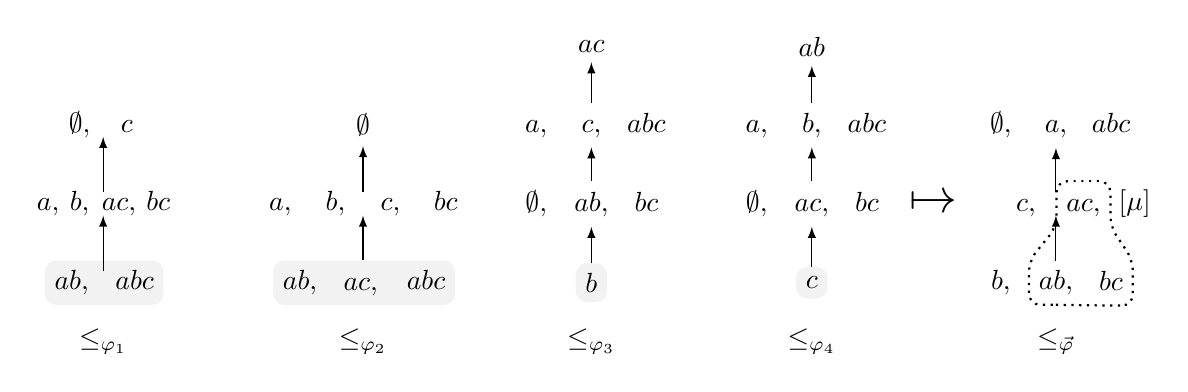
\begin{tikzpicture}
		%% phi1
		\node at (0,-0.75){$\le_{\phi_1}$};

		\node at (-0.4,0)(ab){$ab,$};
		\node at (0.4,0)(abc){$abc\vphantom{,}$};
		\node[inner sep=0.4em] at (0,0)(a1){};
	
		\node at (-0.7,1)(a){$\vphantom{b,}a,$};	
		\node at (-0.3,1)(b){$b,$};		
		\node at (0.2,1)(ac){$\vphantom{b}ac,$};
		\node at (0.7,1)(bc){$bc\vphantom{,}$};
		\node[inner sep=0.4em] at (0,1)(a2){};

		\node at (-0.3,2)(e){$\emptyset,$};
		\node at (0.3,2)(c){$\vphantom{\emptyset,}c$};
		\node[inner sep=0.4em] at (0,2)(a3){};

		\path[-latex] (a1) edge (a2)(a2)edge(a3);
		
		\fill[opacity=0.05, rounded corners=4]
			(ab.south)--(abc.south)--(abc.south east)--(abc.east)--(abc.north east)--(abc.north)--
			(ab.north)--(ab.north west)--(ab.west)--(ab.south west)--(ab.south);


		%% phi2	
		\node at (3.3,-0.75){$\le_{\phi_2}$};

		\node at (2.5,0)(ab){$ab,$};
		\node at (3.3,0)(ac){$ac,\vphantom{\emptyset}$};
		\node at (4.1,0)(abc){$abc\vphantom{,}$};
	
		\node at (2.25,1)(a){$\vphantom{b,}a,$};	
		\node at (2.95,1)(b){$b,$};		
		\node at (3.65,1)(c){$\vphantom{b}c,$};
		\node at (4.35,1)(bc){$bc\vphantom{,}$};
		\node[inner sep=0.4em] at (3.3,1)(a2){};

		\node at (3.3,2)(e){$\emptyset$};
		\node[inner sep=0.4em] at (0,2)(a3){};
	
		\path[-latex] (ac)edge(a2)(a2)edge(e);
		
		\fill[opacity=0.05, rounded corners=4]
			(ab.south)--(abc.south)--(abc.south east)--(abc.east)--(abc.north east)--(abc.north)--
			(ab.north)--(ab.north west)--(ab.west)--(ab.south west)--(ab.south);


		%% phi3	
		\node at (6.2,-0.75){$\le_{\phi_3}$};

		\node at (6.2,0)(b){$b$};

		\node at (5.5,1)(e){$\emptyset,$};
		\node at (6.2,1)(ab){$ab\vphantom{\emptyset},$};
		\node at (6.9,1)(bc){$bc\vphantom{\emptyset,}$};

		\node at (5.5,2)(a){$\vphantom{b,}a,$};	
		\node at (6.2,2)(c){$\vphantom{b}c,$};
		\node at (6.9,2)(abc){$abc\vphantom{,}$};

		\node at (6.2,3)(ac){$ac$};		
	
		\path[-latex] (b)edge(ab)(ab)edge(c)(c)edge(ac);

		\fill[opacity=0.05, rounded corners=4]
			(b.south)--(b.south east)--(b.east)--(b.north east)--(b.north)--
			(b.north west)--(b.west)--(b.south west)--(b.south);


		%% phi4
		\node at (9,-0.75){$\le_{\phi_4}$};

		\node at (9,0)(c){$c$};

		\node at (8.3,1)(e){$\emptyset,$};
		\node at (9,1)(ac){$ac\vphantom{\emptyset},$};
		\node at (9.7,1)(bc){$bc\vphantom{\emptyset,}$};

		\node at (8.3,2)(a){$\vphantom{b}a,$};	
		\node at (9,2)(b){$b,$};
		\node at (9.7,2)(abc){$abc\vphantom{,}$};

		\node at (9,3)(ab){$ab$};		
	
		\path[-latex] (c)edge(ac)(ac)edge(b)(b)edge(ab);

		\fill[opacity=0.05, rounded corners=4]
			(c.south)--(c.south east)--(c.east)--(c.north east)--(c.north)--
			(c.north west)--(c.west)--(c.south west)--(c.south);

		%% arrow
		% \node at (10.55,1.3){$\ssum$};
		\node at (10.55,1){\LARGE $\mapsto$};


		%% sum result
		\node at (12.1,-0.75){$\le_{\P}$};

		\node at (11.4,0)(b){$b,$};
		\node at (12.1,0)(ab){$ab,$};
		\node at (12.8,0)(bc){$bc\vphantom{\emptyset,}$};

		\node at (11.75,1)(c){$c,\vphantom{\emptyset}$};		
		\node[inner sep=0.4em] at (12.1,1)(a2){};
		\node at (12.45,1)(ac){$ac\vphantom{\emptyset},$};

		\node at (11.4,2)(e){$\emptyset,$};
		\node at (12.1,2)(a){$\vphantom{\emptyset}a,$};	
		\node at (12.8,2)(abc){$abc\vphantom{,}$};

		\node at (13.1,1){$[\mu]$};

		\path[-latex] (ab)edge(a2)(a2)edge(a);

		\draw[thick, dotted, rounded corners=4]
			(ab.south)--(bc.south)--(bc.south east)--(bc.east)--(bc.north east)--
			(ac.south east)--(ac.east)--(ac.north east)--(ac.north)--(ac.north west)--
			(ac.west)--(ac.south west)--(ab.north west)--(ab.west)--(ab.south west)--(ab.south);
	\end{tikzpicture}
	\caption{
		Total preorders $\le_{\phi_i}$, for $i\in\{1,2,3,4\}$, 
		corresponding to the opinions of the four Academy members,
		as well as a preorder $\le_{\P}$, 
		corresponding to the profile $\P$.
		As expected, an arrow from $w_1$ to $w_2$ 
		means that $w_1$ is strictly better than $w_2$ in the corresponding preorder,
		while equally preferred interpretations are separated by a comma.
		Note that models of $\phi_i$ are on the bottom, in $\le_{\phi_i}$, 
		i.e., are the most preferred outcomes according to agent $i$.
		The models of the result are the most preferred models of the constraint $\mu$
		(depicted here in the area bordered by the dotted line) in the collective preorder $\le_\P$.
	}
	\label{fig:3-merging-preorder-op-interplay}
\end{figure}

\begin{xmpl}{$\#$OscarsSoFossilized, with preorders}{3-merging-preorder-op-interplay}
	For the setting in Example \ref{ex:3-merging-basic-setup},
	the profile is $\P=(\phi_{1},\phi_{2}, \phi_{3}, \phi_{4})$,
	with
	$\phi_1 = a\land b$,
	$\phi_2 = a\land (b\lor c)$,
	$\phi_3 = \lnot a\land b \land \lnot c$.
	and
	$\phi_4 = \lnot a \land\lnot b\land c$.
	The constraint is $\mu$, 
	with
	$\mu=(a\land b\land \lnot c)\lor (a\land\lnot b\land c)\lor(\lnot a\land b\land c)$.
	Consider, first,
	a total, syntax independent and m-faithful 
	$\L^n$-assignment $\as$ on interpretations
	that assigns to $\P$ and to the formulas in $\P$
	the preorders in Figure \ref{fig:3-merging-preorder-op-interplay}.
	Note that the assignment slice we have presented here 
	is in agreement with properties $\oom{1-9}$.
	According to this assignment
	we obtain that 
	$[\me^{\as}_{\mu}(\P)]=\min_{\le_{\P}}[\mu]=\{ab,bc\}$.

	Conversely, take a merging operator $\me$ such that 
	$[\me_{\px_{ab,bc}}(\P)]=\{ab,bc\}$.
	According to the $\me$-revealed assignemnt,
	we would infer that $ab \approx^{\me}_{\P} bc$,
	which is in accordance with $\le_{\P}$
	as depicted in Figure \ref{fig:3-merging-preorder-op-interplay}.
\end{xmpl}

\subsubsection{Distance-based merging operators}
Standard ways of constructing merging operators 
that satisfy postulates $\ppm{0-8}$
are based on the idea of finding outcomes 
that minimize overall distance to the profile $\P=(\phi_i)_{1\le i \le n}$,
and rely on ingredients that we have encountered before.
The first ingredient is a distance function $\dd$
on interpretations, i.e., a function 
$\dd\colon\U\times\U\rightarrow\mathbb{R}_{\geq 0}$
that satisfies properties $\ood{1-3}$ 
in Section \ref{sec:2-distances}.
Note that, in contrast to revision, update and enforcement,
which only require $\dd$ to be a quasi-distance,
merging requires $\dd$ to be a distance.
The distance $\dd$ 
is then used to generate,
for any propositional formula $\phi$ and interpretation $w$,
the $(\dd,\:\min)$-induced distance $\dd^{\min}(\phi,w)$ 
from a formula $\phi$ to an interpretation $w$,
defined, as usual, as:
$$
	\dd^{\min}(\phi,w)\defeq\min(\dd(v,w))_{v\in[\phi]}.
$$
Following the custom established for the previous belief change 
operators, the $\min$ aggregation function used in the definition
of $\dd^{\min}(\phi,w)$ would count as a second parameter in the 
notation for the anticipated induced merging operator:
however, since the merging operators we will look at in this work
do not rely on any other aggregation functions at this step, 
we will not count it as a distinct modeling choice and
omit it from the list of parameters passed on to the belief change 
function. 
Thus, in the context of merging only, 
we will write $\dd(\phi,w)$ instead of $\dd^{\min}(\phi,w)$.

Based on this notion, we can introduce the 
$\dd$-induced ranking on interpretations, defined,
for any propositional formula $\phi$ and 
interpretations $w_1$ and $w_2$, as:
$$
	w_1 \le^{\dd}_{\phi} w_2~\text{if}~\dd(\phi,w_1)\le \dd(\phi,w_2).
$$
Merging does, nonetheless, appeal to ann aggregation function $\agg$
as a second ingredient, and $\agg$ is expected to 
satisfy properties $\ooa{1-3}$ in Section \ref{sec:2-distances}.
Thus, if 
$\dd$ is a distance between interpretations,
$\agg$ is an aggregation function that satisfies properties $\ooa{1-3}$,
$\P=(\phi_i)_{1\le i \le n}$ is an $\L$-profile 
and $w$ is an interpretation,
the \emph{$(\dd,\:\agg)$-induced distance $\dd^\agg(\P,w)$ from $\P$ to $w$}
is defined as:
$$
	\dd^\agg(\P,w)\defeq\agg(\dd(\phi_{i},w))_{1\le i\le n}.
$$
Consequently, the \emph{$(\dd,\:\agg)$-induced ranking on interpretations} 
is defined, for any profile $\P=(\phi_i)_{1\le i \le n}$
and interpretations $w_1$ and $w_2$, as:
$$
	w_1 \le^{\dd,\:\agg}_{\phi} w_2~\text{if}~\dd^{\agg}(\P,w_1)\le \dd^{\agg}(\phi,w_2).
$$
Note that this definition bears a strong resemblance to the 
definition used for defining the distance from a single formula to 
an interpretation in Section \ref{sec:3-revision},
in that it uses the two parameters of a distance and an aggregation function.
But, as mentioned above, the aggregation function here stands for an extra aggregation
step, such that if we were to follow the overall notational convention 
we would have to use three parameters (one distance function and two aggregation functions).
Since one aggregation function is assumed to be fixed, however,
we omit writing it explicitly.
Note, as well, that if $\phi$ is a propositional formula, then 
$\le_{(\phi)} = \le_{\phi}$.

If $\dd$ is a distance between interpretations
and $\agg$ is an aggregation function,
the \emph{${(\dd,\:\agg)}$-induced $\L^n$-assignment $\as^{\dd,\:\agg}$ on interpretations} 
is obtained by taking 
$\as^{\dd,\:\agg}\!\!(\P)=\le_\phi^{\dd,\:\agg}$,
for any $\L$-profile $\P$.
In the same vein, 
the \emph{${(\dd,\:\agg)}$-induced $\L^n$-merging operator $\me^{\dd,\:\agg}$} 
is the operator induced by the $\L^n$-assignment 
$\as^{\dd,\:\agg}$ on interpretations.
This allows us to generate total, syntax insensitive m-faithful assignments.

\begin{prp}{\cite{KoniecznyP11}}{3-merging-d-agg-induced-preorder}
	If $\dd$ is a distance between interpretations,
	$\agg$ is an aggregation function	
	and $\P=(\phi_i)_{1\le i \le n}$ is an $\L$-profile, 
	the ${(\dd,\:\agg)}$-induced ranking $\le^{\dd,\:\agg}_\P$ 
	satisfies properties $\oom{1-9}$, 
	i.e., $\le^{\agg,\:\min}_\P$ is a total preorder on interpretations that
	is syntax insensitive and is m-faithful.
\end{prp}

Proposition \ref{prop:3-merging-d-agg-induced-preorder} 
implies that the $({\dd,\:\agg})$-induced $\L^n$-assignment
$\as^{\agg,\:\min}$ on interpretations  
is total, m-faithful and syntax insensitive, 
which, by Theorem \ref{thm:3-merging-repr}, 
implies that the $({\dd,\:\agg})$-induced merging operator 
$\me^{\dd,\:\agg}$ satisfies postulates $\ppm{1-6}$.

\begin{crl}{}{3-merging-d-agg-induced-operator}
	If $\dd$ is a distance between interpretations
	and $\agg$ is an aggregation function,
	the $(\dd,\:\agg)$-induced revision operator $\me^{\dd,\:\agg}$ 
	satisfies postulates $\ppm{0-8}$.
\end{crl}

Throughout this work we will typically focus on 
operators generated using Hamming distance $\dd_{\hamming}$
and drastic distance $\dd_{\drastic}$,
and the $\ssum$, $\leximax$ and $\leximin$ aggregation functions,
denoted as $\me^{\hamming,\:\agg}$ and $\me^{\drastic,\:\agg}$,
for $\agg\in\{\ssum,\leximax,\leximin\}$.

\begin{table}\centering
	\begin{tabular}{ccccccccc}
	\cmidrule{2-9}
					  &
					  &
	$[\phi_1]$        &
	$[\phi_2]$        &
	$[\phi_3]$        &
	$[\phi_4]$        &
					  &
					  &
					  \\

					  &
	$\dd_\hamming$  & 
	$\{ab,abc\}$      & 
	$\{ab, ac, abc\}$ & 
	$\{b\}$           & 
	$\{c\}$           &  
	$\leximax$        & 
	$\leximin$        & 
	$\ssum$ 		  \\  	
	\cmidrule{2-9}

					  &
	$\emptyset$       &
	$2$               &
	$2$               & 
	$1$               & 
	$1$               & 
	$(2,2,1,1)$       & 
	$(1,1,2,2)$       & 
	$6$               \\
					  
					  &
	$a$               &
	$1$               &
	$1$               & 
	$2$               & 
	$2$               & 
	$(2,2,1,1)$       & 
	$(1,1,2,2)$       & 
	$6$               \\

	                  &
	$b$               &
	$1$               &
	$1$               & 
	$0$               & 
	$2$               & 
	$(2,1,1,0)$       & 
	$(0,1,1,2)$       & 
	$4$               \\

					  &
	$c$               &
	$2$               &
	$1$               & 
	$2$               & 
	$0$               & 
	$(2,2,1,0)$       & 
	$(0,1,2,2)$       & 
	$5$               \\

	\ldelim\{{3}{1.5em}[${[}\mu{]}$] &
	$ab$              &
	$0$               &
	$0$               & 
	$1$               & 
	$3$               & 
	$(3,1,0,0)$       & 
	$\mathbf{(0,0,1,3)}$       & 
	$\mathbf{4}$               \\

				      &
	$ac$              &
	$1$               &
	$0$               & 
	$3$               & 
	$1$               & 
	$(3,1,1,0)$       & 
	$(0,1,1,3)$       & 
	$5$               \\

					  &
	$bc$              &
	$1$               &
	$1$               & 
	$1$               & 
	$1$               & 
	$\mathbf{(1,1,1,1)}$       & 
	$(1,1,1,1)$       & 
	$\mathbf{4}$               \\

					  &	
	$abc$             &
	$0$               &
	$0$               & 
	$2$               & 
	$2$               & 
	$(2,2,0,0)$       & 
	$(0,0,2,2)$       & 
	$6$               \\
	\cmidrule{2-9}
	\end{tabular}
	\caption{
		Hamming distances from the formulas of the profile $\P$ 
		in Example \ref{ex:3-merging-distance-ops} to each
		interpretation in the universe,
		together with the aggregated distances,
		for the $\leximax$, $\leximin$ and $\ssum$ aggregation 
		functions.
		Models of the constraint $\mu$ are singled out:
		the optimal outcomes are the ones with overall 
		minimal scores.
	}
	\label{tab:3-merging-hamming-distances}
\end{table}

\begin{figure}
	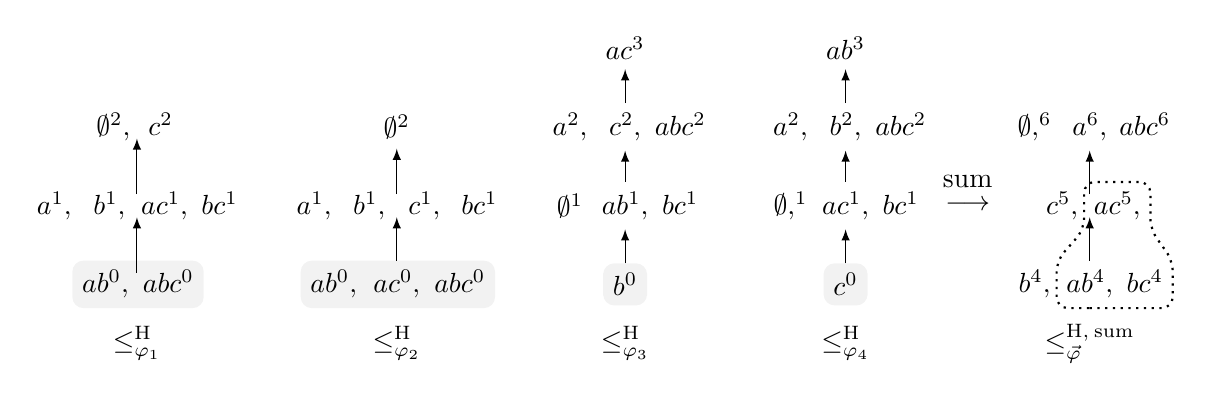
\begin{tikzpicture}
		%% phi1
		\node at (0,-0.75){$\le^{\hamming}_{\phi_1}$};

		\node at (-0.4,0)(ab){$ab^0,$};
		\node at (0.4,0)(abc){$abc^0\vphantom{,}$};
		\node[inner sep=0.4em] at (0,0)(a1){};
	
		\node at (-1.05,1)(a){$\vphantom{b,}a^1,$};	
		\node at (-0.35,1)(b){$b^1,$};		
		\node at (0.35,1)(ac){$\vphantom{b}ac^1,$};
		\node at (1.05,1)(bc){$bc^1\vphantom{,}$};
		\node[inner sep=0.4em] at (0,1)(a2){};

		\node at (-0.3,2)(e){$\emptyset^2,$};
		\node at (0.3,2)(c){$\vphantom{\emptyset,}c^2$};
		\node[inner sep=0.4em] at (0,2)(a3){};

		\path[-latex] (a1) edge (a2)(a2)edge(a3);
		
		\fill[opacity=0.05, rounded corners=4]
			(ab.south)--(abc.south)--(abc.south east)--(abc.east)--(abc.north east)--(abc.north)--
			(ab.north)--(ab.north west)--(ab.west)--(ab.south west)--(ab.south);


		%% phi2	
		\node at (3.3,-0.75){$\le^{\hamming}_{\phi_2}$};

		\node at (2.5,0)(ab){$ab^0,$};
		\node at (3.3,0)(ac){$ac^0,$};
		\node at (4.1,0)(abc){$abc^0\vphantom{,}$};
	
		\node at (2.25,1)(a){$\vphantom{b,}a^1,$};	
		\node at (2.95,1)(b){$b^1,$};		
		\node at (3.65,1)(c){$\vphantom{b}c^1,$};
		\node at (4.35,1)(bc){$bc^1\vphantom{,}$};
		\node[inner sep=0.4em] at (3.3,1)(a2){};

		\node at (3.3,2)(e){$\emptyset^2$};
		\node[inner sep=0.4em] at (0,2)(a3){};
	
		\path[-latex] (ac)edge(a2)(a2)edge(e);
		
		\fill[opacity=0.05, rounded corners=4]
			(ab.south)--(abc.south)--(abc.south east)--(abc.east)--(abc.north east)--(abc.north)--
			(ab.north)--(ab.north west)--(ab.west)--(ab.south west)--(ab.south);


		%% phi3	
		\node at (6.2,-0.75){$\le^{\hamming}_{\phi_3}$};

		\node at (6.2,0)(b){$b^0$};

		\node at (5.5,1)(e){$\emptyset^1$};
		\node at (6.2,1)(ab){$ab^1\vphantom{\emptyset},$};
		\node at (6.9,1)(bc){$bc^1\vphantom{\emptyset,}$};

		\node at (5.5,2)(a){$\vphantom{b,}a^2,$};	
		\node at (6.2,2)(c){$\vphantom{b}c^2,$};
		\node at (6.9,2)(abc){$abc^2\vphantom{,}$};

		\node at (6.2,3)(ac){$ac^3$};		
	
		\path[-latex] (b)edge(ab)(ab)edge(c)(c)edge(ac);

		\fill[opacity=0.05, rounded corners=4]
			(b.south)--(b.south east)--(b.east)--(b.north east)--(b.north)--
			(b.north west)--(b.west)--(b.south west)--(b.south);


		%% phi4
		\node at (9,-0.75){$\le^{\hamming}_{\phi_4}$};

		\node at (9,0)(c){$c^0$};

		\node at (8.3,1)(e){$\emptyset,^1$};
		\node at (9,1)(ac){$ac^1\vphantom{\emptyset},$};
		\node at (9.7,1)(bc){$bc^1\vphantom{\emptyset,}$};

		\node at (8.3,2)(a){$\vphantom{b}a^2,$};	
		\node at (9,2)(b){$b^2,$};
		\node at (9.7,2)(abc){$abc^2\vphantom{,}$};

		\node at (9,3)(ab){$ab^3$};		
	
		\path[-latex] (c)edge(ac)(ac)edge(b)(b)edge(ab);

		\fill[opacity=0.05, rounded corners=4]
			(c.south)--(c.south east)--(c.east)--(c.north east)--(c.north)--
			(c.north west)--(c.west)--(c.south west)--(c.south);

		%% arrow
		\node at (10.55,1.3){$\ssum$};
		\node at (10.55,1){$\longrightarrow$};


		%% sum result
		\node at (12.1,-0.75){$\le^{\hamming,\:\ssum}_{\P}$};

		\node at (11.4,0)(b){$b^4,$};
		\node at (12.1,0)(ab){$ab^4,$};
		\node at (12.8,0)(bc){$bc^4\vphantom{\emptyset,}$};

		\node at (11.75,1)(c){$c^5,$};		
		\node[inner sep=0.4em] at (12.1,1)(a2){};
		\node at (12.45,1)(ac){$ac^5\vphantom{\emptyset},$};

		\node at (11.4,2)(e){$\emptyset,^6$};
		\node at (12.1,2)(a){$\vphantom{\emptyset}a^6,$};	
		\node at (12.8,2)(abc){$abc^6\vphantom{,}$};

		\path[-latex] (ab)edge(a2)(a2)edge(a);

		\draw[thick, dotted, rounded corners=4]
			(ab.south)--(bc.south)--(bc.south east)--(bc.east)--(bc.north east)--
			(ac.south east)--(ac.east)--(ac.north east)--(ac.north)--(ac.north west)--
			(ac.west)--(ac.south west)--(ab.north west)--(ab.west)--(ab.south west)--(ab.south);
	\end{tikzpicture}
	\caption{
		Total preorders $\le^\hamming_{\phi_i}$, for $i\in\{1,2,3,4\}$, 
		corresponding to the opinions of the four Academy members in 
		Example \ref{ex:3-merging-distance-ops},
		as well as the aggregated preorder 
		$\le^{\hamming,\:\ssum}_{\P}$, 
		corresponding to the profile $\P$.
		The models of the result are the 
		most preferred models of the constraint $\mu$
		(depicted here in the area bordered by the dotted line) 
		in the collective preorder $\le_\P$.
		The superscripts next to each interpretation 
		stand for distances; the $\ssum$ aggregation function
		is written above the arrow separating the preorders in the profile
		from the collective preorder $\le^{\hamming,\:\ssum}_{\P}$.
	}
	\label{fig:3-merging-distance-ops}
\end{figure}


\begin{xmpl}{$\#$OscarsSoFossilized, with distances}{3-merging-distance-ops}
	For the setting in Example \ref{ex:3-merging-basic-setup},
	with $\Atoms=\{a,b,c\}$,
	the profile is $\P=(\phi_{1},\phi_{2}, \phi_{3}, \phi_{4})$,
	with
	$\phi_1 = a\land b$,
	$\phi_2 = a\land (b\lor c)$,
	$\phi_3 = \lnot a\land b \land \lnot c$.
	and
	$\phi_4 = \lnot a \land\lnot b\land c$.
	The constraint is $\mu$, 
	with
	$\mu=(a\land b\land \lnot c)\lor (a\land\lnot b\land c)\lor(\lnot a\land b\land c)$.
	The Hamming distances from formulas in the profile $\P$ to each interpretation $w$,
	together with the aggregated distances according to the $\leximax$, $\leximin$
	and $\ssum$ aggregation functions, 
	are depicted in Table \ref{tab:3-merging-hamming-distances}.
	The preorders $\le^{\hamming}_{\phi_{i}}$, as well as the aggregated preorder 
	$\le^{\hamming,\:\ssum}_{\P}$, are depicted in Figure \ref{fig:3-merging-distance-ops}.
	We obtain that:
	$$
		\dd_\hamming(\phi_1,ab)=\min(\dd_\hamming(ab,ab),\dd_\hamming(abc,ab))=\min(0,1)=0,
	$$
	and that:
	$$
		\dd^\ssum_\hamming(\P,ab) = \dd_{\hamming}(\phi_1,ab)+\dd_{\hamming}(\phi_2,ab)
		+\dd_{\hamming}(\phi_3,ab)+\dd_{\hamming}(\phi_4,ab) = 4.
	$$
	With the other aggregation functions, 
	we have that $\dd^\leximax_\hamming(\P,ab) = (3,1,0,0)$,
	i.e., the vector of distances from the formulas in $\P$ to $ab$ ordered in descending order,
	and $\dd^\leximin_\hamming(\P,ab) = (0,0,1,3)$,
	i.e., the vector of distances from the formulas in $\P$ to $ab$ ordered in ascending order.
	Note that 
	$ab \approx^{\hamming,\:\ssum}_{\P} bc$, since $\dd^\ssum_\hamming(\P,ab) = \dd^\ssum_\hamming(\P,bc)$.
	However, the situation is different when using the other aggregating functions:
	$bc <^{\hamming,\:\leximax}_{\P} ab$, since $(1,1,1,1)<_\lex(3,1,0,0)$,
	and $ab <^{\hamming,\:\leximin}_{\P} bc$, since $(0,0,1,3)<_\lex(1,1,1,1)$.
	We obtain that 
	$[\me^{\hamming,\:\leximax}_\mu(\P)]=\{bc\}$,
	$[\me^{\hamming,\:\leximin}_\mu(\P)]=\{ab\}$
	and
	$[\me^{\hamming,\:\ssum}_\mu(\P)]=\{ab,bc\}$.
\end{xmpl}

The operators 
$\me^{\hamming,\:\ssum}$,
$\me^{\hamming,\:\leximax}$
and 
$\me^{\hamming,\:\leximin}$
all embody different attitudes to the aggregation of information.
Intuitively, 
$\me^{\hamming,\:\ssum}$ sees optimal outcomes in utilitarian terms and thereby favors the majority opinion, 
while $\me^{\hamming,\:\leximax}$ attempts to improve the situation of the worse off agent, and usually veers towards egalitarian outcomes;
the $\me^{\hamming,\:\leximin}$ operator is elitist, in that it favors outcomes that improve the situation of the best off agent.
On the other hand, the operators 
$\me^{\drastic,\:\ssum}$, 
$\me^{\drastic,\:\leximax}$
and
$\me^{\drastic,\:\leximin}$,
on the other hand, are all equivalent, i.e., 
$\me^{\drastic,\:\ssum}_\mu(\P)\equiv\me^{\drastic,\:\leximin}_\mu(\P)\equiv\me^{\drastic,\:\leximax}_\mu(\P)$,
for any propositional profile $\P$ and formula $\mu$. 

The difference between majoritarian and egalitarian operators can be hashed out in 
terms of the following postulates \cite{LiberatoreS98,KoniecznyP11}, 
to be thought of in conjunction with postulates $\ppm{0-8}$
and applying for any $\L$-profiles $\P_1$ and $\P_2$,
constraints $\mu$, $\mu_1$ and $\mu_2$, and formulas $\phi_1$ and $\phi_2$:

\begin{description}
	\item[($\ppm{\MAJ}$)] There exists an integer $n$ such that 
		$\me_{\mu}(\P_1+(\underbrace{\P_2+\dots+\P_2}_{n~\text{times}}))\models \me_{\mu}(\P_2)$. 
	\item[($\ppm{\ARB}$)] If $\me_{\mu_1}(\phi_1)\equiv \me_{\mu_2}(\P_2)$,
		$\me_{\mu_1\leftrightarrow\lnot\mu_2}(\phi_1,\phi_2)\equiv \mu_1\leftrightarrow\lnot\mu_2$,
		$\mu_1\not\models\mu_2$ and $\mu_2\not\models\mu_1$,
		then $\me_{\mu_1\lor\mu_2}(\phi_1,\phi_2)\equiv \me_{\mu_1}(\phi_1)$.
\end{description}

Postulate $\ppm{\MAJ}$ says that a large enough coalition 
will sway the merging result in its favor,
while postulate $\ppm{\ARB}$ formalizes the idea that 
the median position is to be preferred \cite{LiberatoreS98}.
We will not delve too much into these properties, 
except to say that operators $\me^{\dd,\:\ssum}$ satisfy postulate $\ppm{\MAJ}$
and operators $\me^{\dd,\:\leximax}$ satisfy postulate $\ppm{\ARB}$.































\section{Related work}\label{sec:3-rw}
Belief change in the sense relevant to us here 
begins, in earnest, with the AGM model of the $1980$s
\cite{AlchourronGM85,AlchourronM85,Gardenfors88},
with some of the main ideas going back,
according to Peter G\"ardenfors \cite{Gardenfors11},
slightly further \cite{Harper76,Levi80}. 

The original AGM publications led to a watershed of works attempting 
to model belief change operators, and revision in particular, in 
more intuitive terms. Important proposals used 
entrenchment relations \cite{GardenforsM88},
systems of spheres \cite{Grove88}
and preorders on possible worlds \cite{KatsunoM92}.
All of these models rely, in some way or another, on 
preferences, either among formulas or interpretations.
The latter reference, of course, provides the basis for our own work,
with a closely related model \cite{KatsunoM91} providing the basis 
for our presentation of update.
It should be mentioned that the AGM model assumes a language 
that subsumes propositional logic, and, as such, is strictly more general 
than the Katsuno-Mendelzon model taken here as reference point. 
Nonetheless, the choice mechanisms that underly revision 
are similar across all representations:
we chose the Katsuno-Mendelzon model 
because, in our opinion, it exhibits these mechanisms in a way that is
intuitive and that lends itself to applications across various other domains.

In the initial AGM model revision was often placed side by side 
with \emph{contraction}, deemed equally important and analysed as a belief 
change operation in its own right. 
Contraction models removals of certain items of knowledge from a bigger corpus:
in the terminology used here, contraction of $\phi$ with respect to $\mu$
would require changing $\phi$ in such a way that $\mu$ is not implied by the result.
Though we have not looked at it here, contraction also
affords an interpretation in terms of choice over interpretations \cite{CaridroitKM17}.
In most formal models contraction and revision are intended to be
inter-definable, with a sizeable literature devoted to finding solutions 
for when they are not \cite{Delgrande08,DelgrandeW10,DelgrandeW13,ZhuangPZ13,ZhuangPZ17}.

Belief revision was understood early on to have many ideas in common
with rational choice \cite{Doyle91,Rott93,Schulte99}, with Hans Rott's book \cite{Rott01}
providing an in-depth analysis of these connections, together with a set of 
bold philosophical claims. Most of the claims presented in Section \ref{sec:3-revision}
can be traced, in some way or another, to this work. Nonetheless, the formal model 
we work with is different, and the results, when not following directly 
from the Katsuno-Mendelzon paper \cite{KatsunoM92}, were derived from scratch.
There are more recent takes on the parallel between revision and rational choice 
\cite{Bonanno09,Arlo-CostaP10,Hansson14}, but our impression is that the Katsuno-Mendelzon model
remains the easiest one to work with. That postulates $\ppr{1}$, $\ppr{3}$ and $\ppr{5-6}$
are essentially the same as the axioms for choice functions circulating in the 
literature on rational choice is, thus, news to no one, and it has even been argued that 
the equivalence is not a coincidence \cite{Olsson03}.

Even Hans Rott's book, in all its comprehenesiveness, only looks at 
single-agent operations, which, in rational choice terms, is 
equivalent to individual decision makers. 
This is undoubtedly because at the time when Hans Rott was writing his book
the framework for merging \cite{LiberatoreS98,KoniecznyP02,KoniecznyM04,KoniecznyP11}
had not yet been fully developed.
As is clear by now, our view is that merging is to revision as social choice 
is to individual rational choice. There is nothing new about this either,
with several publications attempting to build bridges between merging 
and social choice \cite{Meyer01,MeyerGC01,KoniecznyP05,EckertP05,EveraereKM07,EveraereKM14,DiazP17,EveraereKM17}.

Our work on enforcement came out of an attempt to axiomatize enforcement in
abstract argumentation \cite{Baumann12,WallnerNJ17}, but the postulates took on 
a life of their own when formulated in propositional logic. 
The same postulates, we discovered later, had been used to model the dynamics of \emph{desire} 
\cite{DuboisLP17}, though the duality with revision embodied in Equations 
\ref{eq:revision-to-enforcement} and \ref{eq:enforcement-to-revision} had not been explicitly stated.
Since enforcement does not guarantee full acceptance of the new information $\mu$, 
it shares a similarity with \emph{non-prioritized revision} \cite{Hansson99b,HanssonFCF01}
and \emph{belief promotion} operators \cite{SchwindKM18}.
However, since the postulates characterizing enforcement, and in particular, 
its success postulate $\ppe{2}$, are different, enforcement does not coincide 
with any of the proposals in this literature.

A useful comparison can be made with contraction, 
overlooked in this work but which is, as mentioned above,
an important member of the belief change family.
Contraction of a propositional formula $\phi$ by a 
propositional formula $\mu$ can be represented as a choice 
function using the identity $[\phi]\cup\min_{\le_{\phi}}[\lnot\mu]$,
where $\le_{\phi}$ is a familiar, r-faithful preorder on interpretations that 
depends on $\phi$ \cite{CaridroitKM17}. In other words,
the models of the contraction are obtained by adding 
the most plausible models of $\lnot\mu$, according to $\le_{\phi}$,
to the models of $\phi$.
Consider, now, the following example.

\begin{xmpl}{Enforcement vs contraction}{3-enforcement-vs-contraction}
	For a set of atoms $\Atoms=\{a,b\}$, 
	take $[\phi] = \{a\}$ and $[\mu]=\{b\}$. 
	Then the result of enforcing $\mu$
	with respect to $\phi$ is $[\phi\en\mu]=\phi\lor\mu=\{a,b\}$,
	if the enforcement operator $\en$ satisfies postulate $\ppe{2}$.
	On the other hand, contracting $\phi$ with respect to $\mu$ results 
	in the set of interpretations: 
	\begin{align*}
		[\phi]\cup\min_{\le_{\phi}}[\lnot\mu] &= \{a\}\cup\min_{\le_{\phi}}\{\emptyset,a,ab\}\\ 
											  &= \{a\}\cup\{a\}\\ 
											  & = \{a\}.
	\end{align*}
	The latter equality holds because $\le_{\phi}$ is assumed to satisfy the properties 
	of an r-faithful assignment, such that $\min_{\le_{\phi}}\{\emptyset,a,ab\} = \{a\}$.

	Thus, an agent who starts off believing that $a$ is the true state of the world 
	and queries a source that advocates for $b$
	will want to use an enforcement operator if the source is deemed credible enough.
	If, on the other hand, the source is deemed untrustowrthy and the agent wants to remove 
	any information stemming from it, then it will use an contraction operator.
\end{xmpl}

Note that the result of contraction
in Example \ref{ex:3-enforcement-vs-contraction} is the same 
regardless of the particular preorder $\le_{\phi}$ used,
as long as $\le_{\phi}$ satisfies the properties of an r-faithful assignment.
Thus, Example \ref{ex:3-enforcement-vs-contraction} trades on what are uncontroversial 
cases for both enforcement and contraction, i.e., cases in which the result 
is unambiguously determined on the basis of the standard postulates alone.
As such, it highlights the differences in how incoming information is treated 
by the two operations.







\section{Conclusion}\label{sec:3-conclusion} 
This chapter has introduced us 
to the main vehicles of belief change
we will be studying throughout the rest of this work:
revision, update, enforcement and merging.
The defining characteristics of a belief change operator,
we have seen, are the logical postulates used to axiomatize it,
the preferences over outcomes that items of prior information 
are assumed to influence,
and the optimization behavior shown,
through various representation theorems,
to characterize belief change operators.

One of the aims of this chapter has been to show
that belief change operations can be understood
as choice procedures over the space of interpretations.
The poster child for this approach is revision, 
which presents itself as a straightforward analogue
to choice functions studied in rational choice theory
\cite{Sen69,Sen70,GrantvZ09}.
Theorem \ref{thm:3-revision-repr-total}, in particular, 
tells us that an agent revising beliefs $\phi$ along the lines of
postulates $\ppr{1}$ and $\ppr{3-6}$ 
behaves as if it ranks outcomes
in a total preorder $\le_{\phi}$,
and always picks the minimal models of 
of the new information $\mu$ according to $\le_{\phi}$.
Such an agent, then, behaves like a rational agent
choosing the best elements from a given menu of options:
the menu, here, consists of the models of $\mu$, i.e., 
the possible worlds the agent is allowed to believe
in light of new information,
while the best elements are decided with reference to $\le_{\phi}$.
% Thus, a revision operator can be readily seen as a \emph{choice function}
% over sets of interpretations:
Revision postulates $\ppr{1}$ and $\ppr{3}$
are equivalent to properties $\ooch{1}$ and $\ooch{2}$
of a choice function, 
as presented in 
Section \ref{sec:2-choice-functions},
while postulates $\ppr{5}$ and $\ppr{6}$
are roughly equivalent to 
or properties $\ooch{3}$ and $\ooch{4}$, 
or properties $\alpha$ and $\beta$, 
as they are known in the theory of rational choice \cite{Sen69,Sen70}.
Postulate $\ppr{4}$, though it does not have 
an analogue in rational choice theory,
reinforces the parallel by making sure that revision operators
are not sensitive to the syntax of the formulas involved.
Thus, taken together, postulates $\ppr{1}$ and $\ppr{3-6}$ 
characterize choice functions over outcomes 
rationalizable by total preorders:
accordingly, Theorem \ref{thm:3-revision-repr-total} aligns
with standard choice theoretic results \cite{Arrow51,Sen69}.
The main difference 
between rational choice and revision, then, 
lies in the interpretation given to the concepts at play:
a preference order, in rational choice, 
ranks items in terms of their desirability,
whereas in belief change it ranks outcomes in terms of 
their plausibility.

In the wake of this result, we were able to make sense of other 
aspects of belief change through the lens of choice theory.
Theorem \ref{thm:3-revision-repr-partial}
showed that the optimization behavior 
in Theorem \ref{thm:3-revision-repr-total}
can be reproduced just as well with partial orders
instead of total orders.
Theorems \ref{thm:3-update-repr-km-total} and 
\ref{thm:3-update-repr-km-partial} showed that 
update fits nicely into this perspective,
with the choice being distributed across 
preorders induced by every model of 
the prior information $\phi$ 
rather than, as with revision, 
by $\phi$ as a whole.
Section \ref{sec:3-enforcement} introduced us 
to the novel type of belief change we called 
\emph{enforcement},
with Theorem \ref{thm:3-enforcement-repr} showing 
that choice in the case of enforcement assumes a
particular form: an enforcement operator has to 
figure out what models to add to the new information 
$\mu$, rather than what models to discard.
This is choice over outcomes that are not consistent 
with the new information, but choice nonetheless.
Finally, Theorem \ref{thm:3-merging-repr} showed us that 
the choice perspective lends itself naturally to 
belief merging operators, as they can be seen 
as collective choice procedures.

In recasting belief change operators as choice procedures,
postulate $\ppr{2}$, as well as its various incarnations,
i.e., postulates $\ppu{2}$, $\ppe{2}$ or $\ppm{2}$,
has been consistently put aside for separate treatment: 
this is because a belief change operator does not need it 
in order to function as a choice procedure.
As Theorems \ref{thm:3-revision-repr-R2-total}
and \ref{thm:3-revision-repr-R2-partial} show,
what postulate $\ppr{2}$, together with its avatars,
does is to bias the choice relative to $\phi$,
by making sure that models of $\phi$ are given 
priority in the choice process.
This is consistent with a view in which outcomes 
consistent with a belief $\phi$ are considered the 
most plausible states of affairs,
but raises the question as to what other attitudes 
towards these outcomes are reasonable.
This is a question we will tackle in the next chapter.


\chapter{Revision as Biased Choice}\label{ch:4}

Revision operators that satisfy postulate $\ppr{2}$
(besides the more standard postulates $\ppr{1}$ and $\ppr{3-8}$)
can be understood to adopt a particular attitude
towards prior information,
which articulates the policy 
by which the agent's prior information
behaves with respect to new data: 
if new information $\mu$
is consistent with existing beliefs $\phi$, 
then the result of revision is simply $\phi\land\mu$;
in other words, the agent retains its initial beliefs
and simply supplements them with the new item of information,
if it can do so in a consistent way.
Under the choice perspective of belief change 
we have been advocating,
the agent ranks possible outcomes of the revision process
in terms of their plausibility:
in this setting, postulate $\ppr{2}$ 
makes sure that, when beliefs are up for grabs,
models of the prior information $\phi$ are the first in line
to be chosen.
This attitude is in line with a view of revision according to which 
the prior information $\phi$ 
stands for the set of outcomes the agent finds most plausible,
information not to be given up unless challenged
by conflicting new data.
This is a conservative attitude towards initial beliefs,
guided by the desire to preserve them as much as possible.
As pointed out in Section \ref{sec:3-revision},
it is lended support by Peter G\"ardenfors' argument that
information is not cheap and should be preserved to the best
of one's ability \cite[p.\~49]{Gardenfors88}, 
or by Harold Abelson's observation that humans treat beliefs as 
possessions \cite{Abelson86}.
However, it is not the only attitude 
towards the prior information an agent can have.

\begin{figure}\centering
	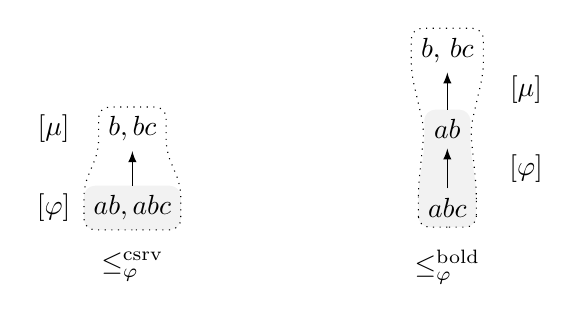
\begin{tikzpicture}
		\node at (0, -0.75){$\le^{\mathrm{\conservative}}_{\phi}$};
		\node at (0,0)(0){$ab,abc$}; 
		\node at (0,1)(1){$b,bc$};
		\node at (-1, 0){$\mods{\phi}$};
		\node at (-1, 1){$\mods{\mu}$};
		\path[-latex] (0) edge (1);
		\fill[opacity = 0.05, rounded corners = 4pt]
			(0.south)--
			(0.south east)--
			(0.east)--
			(0.north east)--
			(0.north)--
			(0.north west)--
			(0.west)--
			(0.south west)--
			(0.south);
		\draw[rounded corners = 4pt, dotted]
			(0.south)--
			(0.south west)--
			(0.west)--
			(0.north west)--
			(1.south west)--
			(1.west)--
			(1.north west)--
			(1.north)--
			(1.north east)--
			(1.east)--
			(1.south east)--
			(0.north east)--
			(0.east)--
			(0.south east)--
			(0.south);

		\node at (4, -0.75){$\le^{\mathrm{bold}}_{\phi}$};
		\node at (4,0)(0){$abc$}; 
		\node at (4,1)(1){$ab$};
		\node at (4,2)(2){$b$, $bc$};
		\node at (5, 0.5){$\mods{\phi}$};
		\node at (5, 1.5){$\mods{\mu}$};
		\path[-latex] (0) edge (1) (1) edge (2);
		\fill[opacity = 0.05, rounded corners = 4pt]
			(0.south)--
			(0.south east)--
			(0.east)--
			(0.north east)--
			(1.south east)--
			(1.east)--
			(1.north east)--
			(1.north)--
			(1.north west)--
			(1.west)--
			(1.south west)--
			(0.north west)--
			(0.west)--
			(0.south west)--
			(0.south);
		\draw[rounded corners = 4pt, dotted]
			(0.south)--
			(0.south west)--
			(0.west)--
			(0.north west)--
			(1.west)--
			(2.south west)--
			(2.west)--
			(2.north west)--
			(2.north)--
			(2.north east)--
			(2.east)--
			(2.south east)--
			(1.east)--
			(0.north east)--
			(0.east)--
			(0.south east)--
			(0.south);
	\end{tikzpicture}
	\caption{
		Two agents start with the same prior information $\phi=a$
		and receive the same new information $\mu=b$,
		but revise according to different preorders:
		$\le^{\conservative}_{\phi}$ is guided by the 
		more conservative imperative of preserving as much
		of the original information as possible;
		$\le^{\bld}_{\phi}$ is bolder, in that it
		considers outcome $abc$ more likely than $ab$, 
		though both are consistent with $\phi$,
		and draws the more specific, though riskier,
		conclusion.
		Models of $\phi$ are shaded in gray,
		models of $\mu$ are surrounded by the dotted line.
	}
	\label{fig:4-asthma-symptoms}
\end{figure}

\begin{xmpl}{The art of diagnosis with biased preferences}{4-asthma-symptoms}
	A patient that has been previously diagnosed with asthma ($a$)
	sees two doctors,
	both of whom are aware of the patient's pre-existing condition.
	After a consultation it emerges that 
	the patient is suffering from shortness of breath ($b$).
	The first doctor revises its beliefs by merely taking in 
	this new information, i.e., concluding
	that the patient suffers from asthma and shortness of breath
	($a\land b$).
	The second doctor infers that chest pain ($c$) 
	must also be present ($a\land b\land c$):
	the two symptoms often go together in asthma, 
	and the doctor is inclined to give added weight 
	to this information.
	The conclusions of both doctors are based on 
	accepting the new information,
	but they follow different strategies: 
	the first doctor is more conservative in the 
	way it uses the new information, 
	whereas the second doctor draws a bolder conclusion.

	Formalizing this as a belief change scenario,
	we would assume
	the alphabet $\Atoms=\{a,b,c\}$
	and two agents, corresponding to the two doctors.
	Both agents are in possession of the same 
	prior information $\phi = a$
	and they both revise
	by the same item of new information $\mu=b$.
	We assume that their revision policies 
	are captured by two $\L$-revision operators 
	$\re^{\conservative}$ and $\re^{\bld}$
	that satisfy postulates $\ppr{1}$ and $\ppr{3-6}$,
	i.e., $\re^{\conservative}$ and $\re^{\bld}$  are exhaustive.
	We know, by Theorem \ref{thm:3-revision-repr-total},
	that this is equivalent to having the doctors
	rank outcomes according to a plausibility order
	specific to each,
	then settle on outcomes
	that are most plausible 
	according to these plausibility orders.
	The first doctor concludes that the patient
	has asthma and shortness of breath,
	i.e., $\phi\re^{\conservative}\mu =a\land b$.
	Note that $\phi\re^{\conservative}\mu\equiv\phi\land\mu$,
	i.e., the first doctor revises in accordance 
	with postulate $\ppr{2}$.
	Since $[\phi\land\mu]=\{ab,abc\}$, this 
	revision policy is equivalent to saying that the
	agent considers outcomes $ab$ and $abc$ equally likely,
	and overall more likely than other models of $\mu$,
	such as $b$ or $bc$.
	Such an attitude is in accordance with an r-faithful 
	$\L$-assignment on interpretations,
	and in particular with properties $\oor{5}$ and $\oor{7}$
	in Section \ref{sec:3-revision}.
	A total preorder $\le^{\conservative}_{\phi}$ consistent with this 
	attitude is depicted on the left in Figure \ref{fig:4-asthma-symptoms}.

	The second doctor concludes that the patient must 
	have chest pain, alongside the 
	already known asthma and shortness of breath,
	i.e., $\phi\re^{\bld}\mu\equiv a\land b\land c$.
	Since $[\phi\land\mu]=\{ab,abc\}$, this 
	revision policy is equivalent to saying that the
	agent considers outcome $abc$ more likely than every other 
	model of $\mu$, including $ab$.
	Such an attitude is not in accordance with an r-faithful 
	$\L$-assignment on interpretations,
	and a total preorder $\le^{\bld}_{\phi}$ consistent with this 
	attitude is depicted on the right in Figure \ref{fig:4-asthma-symptoms}.
	In particular, property $\oor{5}$, saying that models 
	of the prior information $\phi$ should be considered 
	equally likely,
	is not satisfied by $\le^{\bld}_\phi$.
	Nonetheless, in light of its experience, readings
	or hunches, the second doctor is happy to factor in information
	about the relative likelihood of certain outcomes,
	even if it means that they will be at variance with 
	property $\oor{5}$.
\end{xmpl}

Example \ref{ex:4-asthma-symptoms} shows two ways of approaching
revision, based on two ways of ranking outcomes consistent with the
prior information:
a more conservative way, consistent with the familiar postulate $\ppr{2}$,
and a bolder way, more eager to distinguish between such outcomes in terms
of plausibility.
The moral we want to draw from Example \ref{ex:4-asthma-symptoms} 
is not that one of the strategies is 
better, or more rational, than the other, 
since we can, of course, come up with scnearios where 
either of the strategies will fare better than the other.
We also want to resist the conclusion that the right way to model
the difference between these cases is to show that one agent
has access to more information than the other: 
in our setup both agents have access to the same primary information,
$\phi$ and $\mu$; the only thing that differs is the way in which
they rank outcomes consistent with this information.

% One way of thinking
% of postulates $\ppr{1}$ and $\ppr{3-6}$ is that they axiomatize 
% total preorders on interpretations.
% These preorders nominally depend on $\phi$,
% but nothing in postulates $\ppr{1}$ and $\ppr{3-6}$
% touches on how models of $\phi$
% should influence these preorders.
% In other words, there is as yet no information
% about the attitude of an agent towards its initial epistemic state,
% and postulates $\ppr{1}$ and $\ppr{3-6}$ are consistent
% with arbitrary attitudes towards $\phi$.
% including one in which, say, 
% an agent considers models of $\phi$ 
% as the \emph{least} plausible possible worlds.
% Such an attitude towards the models of $\phi$ is, admittedly, 
% extravagant:
% the agent will discard information contained in $\phi$
% at the first possibility to do so. 
% And, while one could be imagine situations in which 
% this behavior makes sense,
% such an attitude challenges the idea that the interpretations
% in $[\phi]$ form the objects of \emph{belief}:
% for, while there is no unanimously agreed upon view about what belief is,
% it can be argued that, at the very least,
% to believe an item of information implies to be partial towards it 
% in certain ways.
% How should the models of $\phi$ stand in relation to
% all other interpretations?
% Example \ref{ex:asthma-symptoms} offers a glimpse into two possible answers:
% the first doctor 
% the agent starts off with some information $\phi$ and differentiates among
% possible worlds consistent with $\phi$: some of these worlds are  more plausible than others,
% perhaps as a result of being more salient, 
% or because of a systematic bias \cite{KahnemanST82}.
% Still, as a whole, models of $\phi$ are more plausible than 
% any \emph{other} interpretations consistent with the new information $\mu$.
% In other words, the agent is biased towards the possible worlds consistent with $\phi$,
% an attitude which fits with the idea of $\phi$ being the agent's \emph{belief}.
% Are there, now, other ways of arranging the models of $\phi$ in $\le_{\phi}$,
% ways that span the space of possible such attitudes?
% We study this question through the lens of additional axioms.

In this chapter we view the attitude
embodied by the standard postulate $\ppr{2}$ 
as one among many that an agent can have 
towards its initial beliefs.
By considering alternatives to
% KM postulate \R{2}, which is 
postulate $\ppr{2}$,
we are able to axiomatize revision operators
that embody a wider range of attitudes towards prior information,
and characterize these operators in terms of the
types of preorders they induce on the set of possible worlds.
To illustrate these principles we provide concrete operators, 
constructed using the ingredients introduced in Section \ref{sec:2-distances}:
a notion of \emph{distance} between interpretations
and an \emph{aggregation function} that ranks possible worlds
depending on the initial beliefs.
We also show, in each case, how these operators fit into the landscape
of new postulates introduced. 
Without the theoretical apparatus of the new postulates,
the concrete operators put forward 
would be merely classified as deviant,
since they do not satisfy 
% KM postulate \R{2}:
the traditional postulate $\ppr{2}$.
But through the present analysis 
they can be viewed as encoding distinct and characterizable 
stances an agent can take towards its beliefs. 

% This chapter is based on work published previously at NMR 2018 \cite{HaretW2018b}
% and IJCAI 2019 \cite{HaretW19a}.

\section{Postulates for biased revision operators}\label{sec:4-postulates}
In Section \ref{sec:3-revision} we presented a set of postulates for revision,
which we divided into several groups.
Postulates $\ppr{1}$ and $\ppr{3-6}$ defined \emph{exhaustive}
revision operators, while postulates $\ppr{1}$, $\ppr{3-5}$ and $\ppr{7-8}$
defined \emph{exclusive} revision operators.
In this chapter we will focus on exhaustive operators,
which, according to Theorem \ref{thm:3-revision-repr-total}, 
are represented by total, syntax insensitive 
$\L$-assignments on interpretations.
The aim here is to hold postulates $\ppr{1}$ and $\ppr{3-6}$ fixed
and explore alternatives to postulate $\ppr{2}$.
We will do this by considering weaker versions of postulate $\ppr{2}$,
as well as postulates that express related, but ultimately different intuitions.

Thus, we put forward the following postulates,
meant to apply to any propositional formulas $\phi$ and $\mu$,
and complete propositional formulas $\dot{\phi}$:

\begin{description}
	\item[($\ppr{9}$)] If $\phi\land\mu$ is consistent, then $\phi\re\mu\models\phi\land\mu$.
	\item[($\ppr{10}$)] If $\phi\land\mu$ is consistent, then $\phi\land\mu\models\phi\re\mu$.
	\item[($\ppr{11}$)] If $\phi\re\mu\models\dual{\phi}$, then $\phi\re\mu\equiv\mu$.
	\item[($\ppr{12}$)] If $\mu\not\models\dual{\phi}$, then $(\phi\re\mu)\land\dual{\phi}$ is inconsistent.
	\item[($\ppr{13}$)] If $\dot{\phi}\models\phi\re\mu$, then $\dot{\phi}\models(\phi\lor\dot{\phi})\re\mu$.
	\item[($\ppr{\NEUT}$)] $\rnm(\phi\re\mu)\equiv\rnm(\phi)\re\rnm(\mu)$.
\end{description}

Each of these postulates encodes a particular type 
of attitude towards prior information,
and they are intended to be thought of in conjunction 
with the basic set of postulates $\ppr{1}$ and $\ppr{3-6}$.
%Notice that, taken together,
%postulates \R{6-7} imply that $\phi\re\mu$ is equivalent to $\phi\land\mu$
%(when $\phi\land\mu$ is consistent).
%This property, alongside postulates \R{1-5}, is 
%typically proposed as the default set of 
%rational properties for revision~\cite{DBLP:journals/ai/KatsunoM92}.
%It should be noted, however, that postulates \R{6-7} 
%embody a particular stance towards initial beliefs $\phi$,
%expounded on below.
%Our purpose in this section is to explore different attitudes 
%an agent can have towards $\phi$,
%and thus we argue for keeping postulates \R{1-5} constant
%and varying the rest.
Postulate $\ppr{9}$ models an agent who reserves the right 
to drop information from $\phi$ if it sees fit to,
even if that information is consistent with $\mu$:
we may imagine this is done on the basis of certain 
preferences over the information encoded by $\phi$,
i.e., the agent is partial towards some of the models 
of $\phi$ to the detriment of others,
along the lines of the second doctor in Example \ref{ex:4-asthma-symptoms}.
This type of discrimination can be explained
by the agent having some background knowledge 
of the relative likelihoods of certain outcomes,
as was the case in Example \ref{ex:4-asthma-symptoms},
or be the result of some heuristic that the agent uses
to process information.

\begin{xmpl}{Steve}{4-heuristic-availability}
	Consider Steve, the subject of a classical example by Daniel Kahneman
	and Amos Tversky:

	\begin{quote}
		An individual has been described by a neighbor as follows: 
		``Steve is very shy and withdrawn, 
		invariably helpful but with little 
		interest in people or in the world of reality. 
		A meek and tidy soul, 
		he has a need for order and structure, 
		and a passion for detail.” 
		Is Steve more likely to be a librarian or a farmer?''
		\cite{Kahneman11}
	\end{quote}
	Most people, we are told, reply that Steve is more likely to be a librarian: 
	they do so based primarily on the stereotypical 
	image of what it is to be a librarian,
	while disregarding more useful facts, such as the statistical distribution of
	librarians versus farmers in the population, which would favor farmers.
	Humans, it seems, readily use a representativeness heuristic to draw 
	conclusions that are otherwise unwarranted.

	Imagine this example simplified to fit the parameters of a quick 
	revision scenario:
	an agent knows that Steve is shy ($a$)
	and learns, in addition, that Steve is helpful and very well organized ($b$).
	The agent concludes that Steve is a librarian ($c$).
	Formally, this example has the same structure as 
	Example \ref{ex:4-asthma-symptoms},
	with prior information $\phi=a$, 
	new information $\mu=b$
	and conclusion $\phi\re\mu\equiv a\land b\land c$,
	and results in the same observation:
	the agent considers the outcome $abc$ more likely than outcome $ab$.
	But this time it is on the basis of an availability bias:
	outcome $abc$ is simply more salient in the agent's mind
	than $ab$ alone, even though they are both consistent with $\phi$ and $\mu$.
	Who are we to judge?
\end{xmpl}

Postulate $\ppr{10}$ refers to an attitude that is, in some ways, 
the oposite of the attitude in postulate $\ppr{9}$: it models an agent who 
incorporates all information in $\phi\land\mu$, 
and possibly extends this to cover more ground.
Taken together, postulates $\ppr{9}$ and $\ppr{10}$ 
imply that $\phi\re\mu$ is equivalent to $\phi\land\mu$, when $\phi\land\mu$ is consistent,
i.e., they are equivalent to the classical postulate $\ppr{2}$.

% This property models an agent 
% who wants to preserve as much of $\phi$ as it can,
% and does not have any bias towards either of the models of $\phi$.
% In the KM postulatestization $\ppr{7}$ and $\ppr{8}$ are packaged together in one postulate
% (i.e., KM postulate $\ppr{2}$) and presented alongside $\ppr{1}$ and $\ppr{3-6}$ as 
% the default set of rational properties for revision \cite{KatsunoM92}.

Postulates $\ppr{11}$ and $\ppr{12}$ focus on the dual formula $\dual{\phi}$
obtained by replacing every literal in $\phi$ with its dual, 
i.e., negated version (see Section \ref{sec:2-prop-logic}).
Why are these formulas significant?
Note that in certain special cases, 
such as when $\phi$ is a conjunction of literals 
or a complete formula (i.e., with exactly one model),
then $\dual{\phi}$ will be a formula whose models are complements of the models of $\phi$.

\begin{xmpl}{Dual formulas as opposite points of view}{4-dual-formula-specific}
	For the set of atoms $\Atoms=\{a,b,c\}$,
	consider formulas 
	$\phi_1 = a\land b\land \lnot c$,
	$\phi_2 = a\land b$,
	$\phi_3 = a\lor b$,
	$\phi_4 = b\rightarrow c$.
	We have that 
	$\dual{\phi_1}=\lnot a\land \lnot b\land c$
	and 
	$\dual{\phi_2} = \lnot a \land \lnot b$,
	with
	$[\phi_1]=\{ab\}$ and $[\phi_2]=\{ab, abc\}$
	while $[\dual{\phi_1}]=\{c\}$ and $[\dual{\phi_2}]=\{\emptyset,c\}$.
	On the other hand, 
	$[\phi_3]=\{a,b,ab,ac,bc,abc\}$ and $[\phi_4]=\{\emptyset,a,c,ac,bc,abc\}$,
	while
	$[\dual{\phi_3}]=\{\emptyset,a,b,c,ac,bc\}$ and $[\dual{\phi_4}] = \{\emptyset,a,b,ab,bc,abc\}$.
	Note that $[\phi_1]\cap[\dual{\phi_1}]=\emptyset$ and $[\phi_2]\cap[\dual{\phi_2}]=\emptyset$,
	but
	$[\phi_3]\cap[\dual{\phi_3}]=\{a,b,ac,bc\}$ 
	and 
	$[\phi_4]\cap[\dual{\phi_4}]=\{\emptyset,a,bc,abc\}$.
\end{xmpl}

Conjunctions of literals or complete formulas can be thought of as being very specific,
in the sense that they model agents with definite opinions on some (or all) atoms.
In this case, $\dual{\phi}$ can be thought of as the point of view opposite to that of $\phi$,
i.e., the outcome least likely to be true if $\phi$ is.
As Example \ref{ex:4-dual-formula-specific} illustrates, however,
this analogy breaks down if $\phi$ is a different type of formula, such as a disjunction or a conditional.
In this case $\phi$ and $\dual{\phi}$ can share models, and the distinction between a formula and its dual
is not as clear-cut anymore.
The claim, then, is only that there are situations in which 
it makes sense to view $\phi$ and $\dual{\phi}$
as embodying opposing stances,
and situations can be imagined in which it is desirable to put bounds on the revision
function in terms of how it treats information encoded by $\dual{\phi}$.
This is the case if the agent has, or is required to have, a definite opinion on every item from an agenda,
as is typically the case in Judgment Aggregation~\cite{Endriss16};
if $\phi$ is a `vivid' formula~\cite{Levesque86};
or, if it encodes something like an agent's preferred bundle from a set of available items.
In all these cases $\phi$ can be required to be a conjunction of literals or a complete formula.
%For our purposes, postulates \ppr9-10} 
%place some bounds on 
%the revision output in terms of the information
%represented by this foreign point of view.
In this context, postulate $\ppr{11}$ says that if $\phi$ undergoes revision by 
a formula $\mu$ embodying such an adverse perspective,
then the agent must adopt $\mu$:
in other words, the agent has no room for maneuvering towards a more amenable middle ground.
% Though this sounds like an odd revision policy,
Such a revision policy makes more sense when considered alongside postulate $\ppr{12}$, %\ppr10},
which specifies that if the agent has the option of believing
states of affairs \emph{not} compatible with $\dual{\phi}$,
it should wholeheartedly adopt those as the most plausible stance.
Taken together, postulates $\ppr{11}$ and $\ppr{12}$
inform the agent to believe states of affairs
compatible with $\dual{\phi}$ only if it has no other choice in the matter:
the models of $\dual{\phi}$
should be part of a viewpoint one is willing to accept
only as a last resort. 

\begin{xmpl}{Recommending as revising}{4-online-recommender}
	Consider an online streaming platform that gathers data about its users
	in order to tailor recommendations to their likes and preferences.
	Suppose $\phi$ encodes something like the information this system 
	has about a specific user (e.g., the items that the user liked), 
	$\mu$ represents a query from the user
	and $\phi\re\mu$ represents the set of results suggested to the user by 
	the online platform, in response to the query $\mu$.

	We can imagine that the platform uses its knowledge $\phi$ to construct 
	a profile of the user, which then serves as guide about what to recommend:
	in revision terms, this profile serves as the revision policy, or, 
	as we will soon see, a ranking of the possible outcomes.
	We can also imagine that it is important for the platform that 
	this profile contains, besides the items that the 
	user is most likely to appreciate, also a list of items that the user will 
	\emph{dislike}, so as to avoid suggesting those as much as possible
	(i.e., unless the user explicitly requests them).
	In revision terms, we can conceptualize this as a set of interpretations that 
	are in the result $\phi\re\mu$ only as a last resort,
	and it is not difficult to see that the duals of the `liked' outcomes 
	are good candidates for these, likely to be loathed, options.
\end{xmpl}

Postulate $\ppr{13}$ enforces coherence of change 
when the prior information includes some element that would have been chosen in a different state of mind,
and is best understood through an example.

\begin{xmpl}{So many options}{4:R13}
	An agent intends to go to an art museum ($a$),
	the beach ($b$) and a concert ($c$),
	encoded as the complete propositional formula $\phi=a\land b\land c$,
	with the set of atoms $\Atoms=\{a,b,c\}$.
	The agent then learns that it only has time
	for one of these activities: this is encoded as newly acquired information
	$\mu = (a\land\lnot b\land \lnot c)\lor (\lnot a\land b\land \lnot c)\lor (\lnot a\land\lnot b\land c)$,
	with $[\mu]=\{a,b,c\}$.
	The agent chooses the art museum $a$, i.e.,
	$\phi\re\mu\equiv\dot{\phi}\equiv a\land\lnot b\land\lnot c$.
	Note that $\dot{\phi}\models\phi\re\mu$.
	If the agent's initial intentions had been more inclusive
	in the sense that it would have expressed a willingness to do either all three activities
	or just visit the museum, 
	encoded as $\phi\lor\dot{\phi}$,
	then, faced with the same new information $\mu$, 
	the option of going to the art museum
	(i.e., $a\land\lnot b\land\lnot c$) should still feature as one of its most preferred options.
\end{xmpl}

We have also found it suitable to add here a neutrality postulate $\ppr{\NEUT}$, 
requiring that a revision operator does not favor propositional atoms based solely on their names.
This idea is expressed by requiring the revision output to be invariant under a renaming $\rnm$ of atoms,
and, in conjunction with the insensitivity to syntax postulate $\ppr{4}$,
it is perhaps natural to expect it from any revision operator.
The inspiration for postulate $\ppr{\NEUT}$ is
the social choice literature
and, though it has appeared in belief change before, 
under various guises~\cite{HerzigR99,MarquisS14,HaretPW16}, 
neutrality usually goes unstated in standard presentations of revision.

\section{Biased preferences over outcomes}\label{sec:4-assignments}
A clearer view of postulates $\ppr{9-13}$ and $\ppr{\NEUT}$
emerges when looking at the constraints they impose on how models of $\phi$
are placed in the preorder $\le_\phi$.
That is to say, we assume an agent with prior information $\phi$ ranks interpretations
in a total preorder $\le_\phi$,
i.e., that there exists a total, syntax insensitive $\L$-assignment 
$\as$ on interpretations
that satisfies properties $\oor{1-4}$, as presented in Section \ref{sec:3-revision}.
The additional constraints we want to consider in this chapter
are expressed in the following properties,
applying for any interpretations $w_1$, $w_2$ and $v$
and propositional formulas $\phi$ and $\px_v$, where $[\px_v]=\{v\}$:

\begin{description}
	\item[($\oor{7}$)] If $w_1\in[\phi]$ and $w_2\notin[\phi]$, then $w_1<_\phi w_2$.

	\item[($\oor{8}$)] If $w_1\in[\phi]$, then $w_1\le_\phi w_2$.
		
	\item[($\oor{9}$)] If $w_1\in[\dual{\phi}]$, then $w_2\le_\phi w_1$.
	
	\item[($\oor{10}$)] If $w_1\in[\dual{\phi}]$ and $w_2\notin[\dual{\phi}]$, then $w_2<_\phi w_1$.
	
	\item[($\oor{11}$)] If $v\le_\phi w$, then $v\le_{\phi\lor\px_v} w$.
	
	\item[($\oor{\NEUT}$)] If $w_1\le_\phi w_2$, then $\rnm(w_1)\le_{\rnm(\phi)}\rnm(w_2)$.	
\end{description}

% A revision operator is \emph{basic} if it satisfies postulates 
% $\ppr{1,3-5}$ and \emph{neutral} if it satisfies postulate $\ppr\NEUT$.
\begin{figure}\centering
	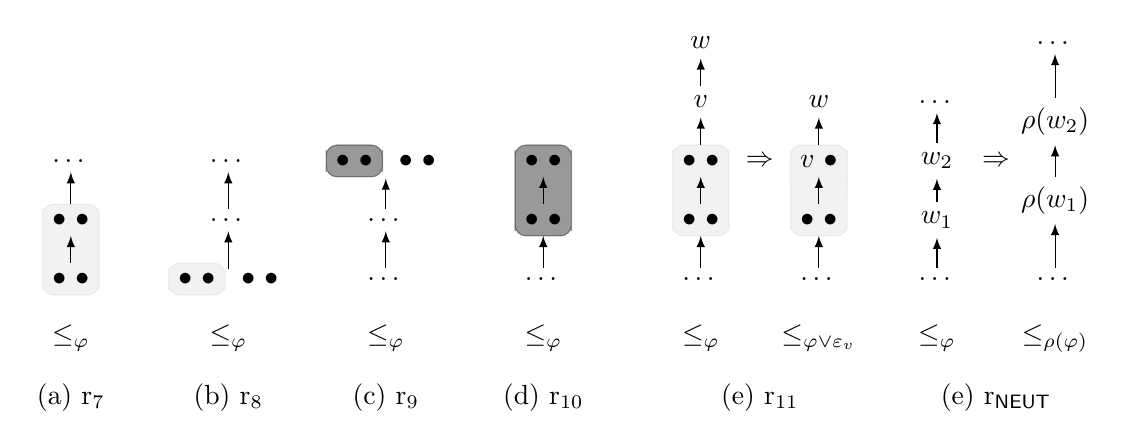
\begin{tikzpicture}
		\node at (0,-1.5){(a) $\oor{7}$}; 
		\node at (0,-0.75){$\le_\phi$};
		\node at (0,0)(0){$\bullet~\bullet$};
		\node at (0,0.75)(1){$\bullet~\bullet$};
		\node at (0,1.5)(2){\dots};
		\path[-latex] (0) edge (1)(1) edge (2);
		\fill[draw, opacity=0.05, rounded corners=4pt]
		(0.south)--
		(0.south west)--
		(0.west)--
		(1.west)--
		(1.north west)--
		(1.north)--
		(1.north east)--
		(1.east)--
		(0.east)--
		(0.south east)--
		(0.south);

		\node at (2,-1.5){(b) $\oor{8}$}; 
		\node at (2,-0.75){$\le_\phi$};
		\node at (1.6,0)(0){$\bullet~\bullet$};
		\node at (2.4,0)(1){$\bullet~\bullet$};
		\node at (2,0)(a1){};
		\node at (2,0.75)(2){\dots};
		\node at (2,1.5)(3){\dots};
		\path[-latex] (a1) edge (2)(2) edge (3);
		\fill[draw, opacity=0.05, rounded corners=4pt]
		(0.north)--
		(0.north east)--
		(0.east)--
		(0.south east)--
		(0.south)--
		(0.south west)--
		(0.west)--
		(0.north west)--
		(0.north);

		\node at (4,-1.5){(c) $\oor{9}$}; 		
		\node at (4,-0.75){$\le_\phi$};
		\node at (3.6,1.5)(0){$\bullet~\bullet$};
		\node at (4.4,1.5)(1){$\bullet~\bullet$};
		\node at (4,1.4)(a1){};
		\node at (4,0.75)(2){\dots};
		\node at (4,0)(3){\dots};
		\path[-latex] (2) edge (a1)(3) edge (2);
		\fill[draw, opacity=0.4, rounded corners=4pt]
		(0.north)--
		(0.north east)--
		(0.east)--
		(0.south east)--
		(0.south)--
		(0.south west)--
		(0.west)--
		(0.north west)--
		(0.north);

		\node at (6,-1.5){(d) $\oor{10}$}; 		
		\node at (6,-0.75){$\le_\phi$};
		\node at (6,1.5)(0){$\bullet~\bullet$};
		\node at (6,0.75)(1){$\bullet~\bullet$};
		\node at (6,0)(2){\dots};
		\path[-latex] (2) edge (1)(1) edge (0);
		\fill[draw, opacity=0.4, rounded corners=4pt]
		(0.north)--
		(0.north west)--
		(0.west)--
		(1.west)--
		(1.south west)--
		(1.south)--
		(1.south east)--
		(1.east)--
		(0.east)--
		(0.north east)--
		(0.north);

		\node at (8.75,-1.5){(e) $\oor{11}$}; 		
		\node at (8,-0.75){$\le_\phi$};
		\node at (8,0)(d){\dots};
		\node at (8,0.75)(k1){$\bullet~\bullet$};
		\node at (8,1.5)(k2){$\bullet~\bullet$};
		\node at (8,2.25)(wp){$v$};
		\node at (8,3)(w){$w$};
		
		\node at (8.75, 1.5){$\Rightarrow$};
		
		\node at (9.5,-0.75){$\le_{\phi\lor\px_v}$};		
		\node at (9.5,0)(d1){\dots};
		\node at (9.5,0.75)(wp1){$\bullet~\bullet$};
		\node at (9.5,1.5)(wp2){$v~\bullet$};
		\node at (9.5,2.25)(w1){$w$};
		
		\path[-latex] 
		(d)edge(k1)(k1)edge(k2)(k2)edge(wp)(wp) edge (w)
		(d1)edge(wp1)(wp1)edge(wp2)(wp2)edge(w1);
		\fill[draw, opacity=0.05, rounded corners=4pt]
		(k1.south)--(k1.south west)--(k1.west)--(k2.west)--
		(k2.north west)--(k2.north)--(k2.north east)--
		(k2.east)--(k1.east)--(k1.south east)--(k1.south);
		\fill[draw, opacity=0.05, rounded corners=4pt]
		(wp1.south)--(wp1.south west)--(wp1.west)--(wp2.west)--
		(wp2.north west)--(wp2.north)--(wp2.north east)--
		(wp2.east)--(wp1.east)--(wp1.south east)--(wp1.south);

		\node at (11.75,-1.5){(e) $\oor{\NEUT}$}; 		
		\node at (11,-0.75){$\le_\phi$};
		\node at (11,0)(d){\dots};
		\node at (11,0.75)(1){$w_1$};
		\node at (11,1.5)(2){$w_2$};
		\node at (11,2.25)(3){\dots};
		
		\path[-latex]
			(d)edge(1)(1)edge(2)(2)edge(3);

		\node at (11.75, 1.5){$\Rightarrow$};
		
		\node at (12.5,-0.75){$\le_{\rnm(\phi)}$};		
		\node at (12.5,0)(d){\dots};
		\node at (12.5,1)(1){$\rnm(w_1)$};
		\node at (12.5,2)(2){$\rnm(w_2)$};
		\node at (12.5,3)(3){\dots};

		\path[-latex]
			(d)edge(1)(1)edge(2)(2)edge(3);
	\end{tikzpicture}
	\caption{
		Schematic view of prototypical preorders
		satisfying each of the properties $\oor{6-10}$;
		models of $\phi$ are in the light gray area,
		models of $\dual{\phi}$ are in the dark gray area.}
	\label{fig:4-biased-preorders-schematic}	
\end{figure}

Each of properties $\oor{7-11}$ tells us something about how prior information $\phi$ 
biases a plausibility ordering over outcomes, especially with regards to the outcomes consistent with $\phi$ 
(i.e., models of $\phi$),
whereas the neutrality property $\oor{\NEUT}$ 
tells us something about the kind of bias the ordering should avoid.
A schematic view of these preorders is offered in 
Figure \ref{fig:4-biased-preorders-schematic}.
Property $\oor{7}$, depicted in Figure~\ref{fig:4-biased-preorders-schematic}-(a), 
says that models of $\phi$ are generally considered
more plausible than interpretations that do not satisfy $\phi$,
but models of $\phi$ themselves may not be equally plausible relative to each other.
Property $\oor{7}$ is familiar from Section \ref{sec:3-revision}, though 
there it was always considered in conjunction with
$\oor{5}$ or $\oor{6}$, and never by itself. Here we shine a spotligh on it alone.
Property $\oor{8}$, depicted in Figure~\ref{fig:4-biased-preorders-schematic}-(b), says that
models of $\phi$ are minimal elements in $\phi$, 
though possibly not uniquely so.
Note that property $\oor{8}$ implies property $\oor{6}$ (see Section \ref{sec:3-revision}),
which says that models of $\phi$ should be equally plausible in $\le_\phi$:
however, $\oor{8}$ tells us more than $\oor{5}$:
it tells us that the agent not only considers models of $\phi$ as equally plausible,
but also at least as plausible as any other outcome.
Properties $\oor{9-10}$, depicted in Figure~\ref{fig:4-biased-preorders-schematic}-(c,d),
say that models of the dual formula $\phi$ are the least plausible interpretations in $\le_\phi$,
while property $\oor{11}$, depicted in Figure~\ref{fig:4-biased-preorders-schematic}-(e),
says that if $v$ is more plausible than $w$ when
the initial beliefs are $\phi$, then $v$ would still be more plausible 
than $w$ if it were part of the initial beliefs.
Lastly, the neutrality property $\oor{\NEUT}$ says that the ranking $\le_\phi$ should be invariant
when renaming the atoms.

Note that properties $\oor{7-8}$, together,
are equivalent to property $\oor{6}$, presented in Section \ref{sec:3-revision}.
Thus, properties $\oor{7-8}$
together with the standard properties 
$\oor{1-5}$ define what is more commonly known as 
a \emph{faithful assignment} \cite{KatsunoM92},
or, as we have named it here,
a total, syntax independent r-faithful $\L$-assignment on interpretations.
Such an assignment
places all and only models of $\phi$ on the lowest level of $\le_\phi$,
and corresponds to an agent for which outcomes 
consistent with its prior belief are the most plausible states of affairs.
This attitude, as is apparent here, 
arises out of a combination of two attitudes that can be looked at separately.

Properties $\oor{7-11}$ and $\oor{\NEUT}$ 
turn out to characterize postulates $\ppr{9-13}$ and $\ppr{\NEUT}$ 
on the semantic level,
as per the following representation result.
Recall that an $\L$-revision operator $\re$ is
represented by an $\L$-assignment $\as$ on interpretations
if $[\phi\re \mu] = \min_{\le_\phi}[\mu]$, for any propositional formulas $\phi$ and $\mu$,
and that, by Theorem \ref{thm:3-revision-repr-total},
if $\re$ is exhaustive, then there always exists a total
assignment $\as$ (i.e., such that $\le_\phi$ is a total preorder) representing it.
Recall, as well, that the $\L$-proxy of a pair $\{w_1,w_2\}$ of interpretations is
a propositional formula $\px_{1,2}$ 
for which $[\px_{1,2}]=\{w_1,w_2\}$.

\begin{thm}{}{4-biased-revision-repr}
	If $\re$ is revision operator that 
	satisfies postulates $\ppr{1}$ and $\ppr{3-6}$
	(i.e., is exhaustive)
	and $\as$ is a total, syntax insensitive 
	$\L$-assignment on interpretations
	that represents it,
	then the following equivalences hold:
	\begin{description}
		\item[(1)] $\re$ satisfies postulate $\ppr{9}$ iff $\as$ satisfies property $\oor{7}$;
		\item[(2)] $\re$ satisfies postulate $\ppr{10}$ iff $\as$ satisfies property $\oor{8}$;
		\item[(3)] $\re$ satisfies postulate $\ppr{11}$ iff $\as$ satisfies property $\oor{9}$;
		\item[(4)] $\re$ satisfies postulate $\ppr{12}$ iff $\as$ satisfies property $\oor{10}$;
		\item[(5)] $\re$ satisfies postulate $\ppr{13}$ iff $\as$ satisfies property $\oor{11}$;
		\item[(6)] $\re$ satisfies postulate $\ppr{\NEUT}$ iff $\as$ satisfies property $\oor{\NEUT}$.
	\end{description}
\end{thm}

\begin{prf*}{}{}%
	We start with Equivalence 1 and show each direction in turn.

	(``$\Leftarrow$'')
	Take a total $\L$-assignment $\as$ on interpretations 
	satisfying property $\oor{7}$
	and the revision operator $\re$ represented by it.
	We want to show that $\re$ satisfies postulate $\ppr{9}$,
	and start by assuming that $\phi\land\mu$ is consistent.
	This implies that $\mu$ is consistent and, by postulate $\ppr{3}$,
	that $\phi \re \mu$ is consistent as well.
	Take, then, an interpretation $w$ such that $w\in[\phi\re\mu]$,
	and suppose $w\notin[\phi\land\mu]$.
	Since $[\phi\re\mu]=\min_{\le_\phi}[\mu]$,
	we obtain that $w\in\min_{\le_\phi}[\mu]$
	and hence $w\in[\mu]$.
	Thus, the fact that $w\notin[\phi\land\mu]$
	implies that $w\notin[\phi]$.
	But, by assumption, it holds that $[\phi\land\mu]\neq\emptyset$,
	which means that there exists $w'\in[\phi\land\mu]$
	and, by property $\oor{7}$, it follows that $w'<_\phi w$.
	But we also have that $w\in\min_{\le_\phi}[\mu]$:
	since $\le_\phi$ is total, this implies that $w \le_\phi w'$: we have arrived at a contradiction.
	
	(``$\Rightarrow$'')
	Take an exhaustive revision operator $\re$ additionally satisfying postulate $\ppr{9}$
	and a total $\L$-assignment $\as$ on interpretations that represents it.
	To show that $\le_\phi$ satisfies property $\oor{7}$, 
	take interpretations $w_1$ and $w_2$ such that $w_1\in[\phi]$
	and $w_2\notin[\phi]$.
	We then have that $\phi\land\px_{1,2}$ is consistent
	and hence, by postulate $\ppr{9}$,
	that $\phi\re\px_{1,2}\models\phi\land\px_{1,2}$.
	Since $[\phi\re\px_{1,2}]$ is, by postulates $\ppr{1}$ and $\ppr{3}$,
	a non-empty subset of $[\px_{1,2}]=\{w_1,w_2\}$,
	we have that at least one of $w_1$ and $w_2$ is in $[\phi\re\px_{1,2}]$.
	Notice, now, that we cannot have $w_2\in[\phi\re\px_{1,2}]$,
	since it would follow that $w_2\in\mods{\phi\land\px_{1,2}}$ and,
	\emph{a fortiori}, that $w_2\in[\phi]$,
	which contradicts a previous finding.
	Thus, $[\phi\re\px_{1,2}]=\set{w_1}$.
	Since $\le_\phi$ represents $\re$, 
	we have that
	$[\phi\re\px_{1,2}]=\min_{\le_\phi}[\px_{1,2}]=\{w_1\}$,
	i.e., that $w_1<_\phi w_2$.		
	
	For Equivalence 2, we show again each direction in turn.

	(``$\Leftarrow$'')
	Take, first, a total $\L$-assignment $\as$ on interpretations 
	satisfying property $\oor{8}$,
	and the revision operator $\re$ represented by it.
	% We want to show that $\re$ satisfies postulate $\ppr{10}$.
	Assuming that $\phi\land\mu$ is consistent,
	we want to show that for any $w_1\in[\phi\land\mu]$, it holds that $w_1\in[\phi\re\mu]$ as well.
	Since $\re$ is represented by $\as$, this is equivalent to showing that
	$w\in\min_{\le_\phi}[\mu]$.
	Take, then, an interpretation $w\in[\phi\land\mu]$,
	and an arbitrary interpretation $w'\in[\mu]$.
	Applying property $\oor{8}$, we infer that $w_1 \le_\phi w_2$,
	which then implies that $w\in\min_{\le_\phi}[\mu]$.

	(``$\Rightarrow$'')
	Take an exhaustive revision operator $\re$ that additionally satisfies postulate $\ppr{10}$,
	and a total $\L$-assignment $\as$ on interpretations that represents it.
	To show that $\le_\phi$ satisfies property $\oor{8}$,
	take two interpretations $w_1$ and $w_2$
	such that $w_1\in[\phi]$. 
	Then, by postulate $\ppr{10}$, we have that 
	$\phi\land\px_{1,2}\models\phi\re\px_{1,2}$.
	This implies that $w_1\in[\phi \re \px_{1,2}]$,
	i.e., that $w_1\in\min_{\le_\phi}[\px_{1,2}]$.
	Thus, it holds that $w_1\le_\phi w_2$.

	Equivalences 3 and 4 are analogous to 1 and 2, respectively.
	For Equivalence 5, assume first that postulate $\ppr{13}$ holds,
	and take interpretations $w$ and $v$ and a formula
	$\dot{\phi}$ such that
	$v\le_\phi w$ and $[\dot{\phi}]=\{v\}$.
	To show that $v\le_{\phi\lor\dot{\phi}}w$,
	we must show that $v\in[(\phi\lor\dot{\phi})\re\px_{v,w}]$,
	where $\px_{v,w}$ is a formula such that
	$[\px_{v,w}] = \{v,w\}$. This follows immediately 
	by applying postulate $\ppr{13}$.
	Conversely, suppose $[\dot{\phi}]=\{v\}$,
	and take $w\in[\phi\re\mu]$.
	Then, we get that $v\le_\phi w$, and we can apply property $\oor{11}$
	to derive the conclusion.
	
	For Equivalence 6, recall that applying a renaming $\rnm$ to a set $\W$ of interpretations
	simply applies $\rnm$ to every interpretation in $\W$, such that 
	if $w\in\W$, then it holds that $\rnm(w)\in\rnm(\W)$.
	We will also make extensive use of 
	Proposition \ref{prop:2-renamings-commute} from Section \ref{sec:2-prop-logic},
	saying that the renaming functions commutes across the semantic line,
	i.e., $[\rnm(\phi)] = \rnm([\phi])$, for any propositional formula $\phi$.
	We again take each direction in turn.
	
	(``$\Rightarrow$'')
	Take an exhaustive revision operator $\re$ that additionally satisfies postulate $\ppr{\NEUT}$,
	and a total $\L$-assignment $\as$ on interpretations that represents it.
	%	By postulate \R{\N}\ we get that:
	%	\begin{align*}
	%	\rnm{\min_{\le_{\phi}}[\mu]} &=\min_{\le_{\rnm{\phi}}}\rnm([\mu]).&
	%	\end{align*}
	Take interpretations $w_1$ and $w_2$ and suppose that $w_1\le_\phi w_2$.
	Then $w_1\in[\phi\re\px_{1,2}]$,
	and hence $\rnm(w_1)\in\rnm([\phi\re\px_{1,2}])$.
	By Proposition \ref{prop:2-renamings-commute},
	we obtain that $\rnm(w_1)\in[\rnm(\phi\re\px_{1,2})]$
	and by postulate $\ppr{\NEUT}$ it follows that 
	$\rnm(w_1)\in[\rnm(\phi)\re\rnm(\px_{1,2})]$.
	This implies that 
	$\rnm(w_1)\in\min_{\le_{\rnm(\phi)}}[\rnm(\px_{1,2})]$,
	which by Proposition \ref{prop:2-renamings-commute} 
	implies that 
	$\rnm(w_1)\in\min_{\le_{\rnm(\phi)}}\rnm([\px_{1,2}])$.
	Thus, $\rnm(w_1)\le_{\rnm(\phi)}\rnm(w_2)$.	
	% Conversely, suppose that $\rnm(w_1)\le_{\rnm(\phi)}\rnm(w_2)$.
	% This implies that 
	% $\rnm(w_1)\in\min_{\le_{\rnm(\phi)}}\rnm([\px_{1,2}])$.
	% By Proposition \ref{prop:renaming-commute} and 
	% postulate $\ppr{\NEUT}$,
	% we get that $w_1\le_\phi w_2$.

	(``$\Leftarrow$'')
	Take a total $\L$-assignment $\as$ on interpretations 
	that satisfies property $\oor{\NEUT}$
	and the revision operator $\re$ represented by it.
	By Proposition \ref{prop:2-renamings-commute}
	we have that 
	$
	[\rnm(\phi\re\mu)]=
	\rnm([\phi\re\mu])=
	\rnm(\min_{\le_{\phi}}[\mu])
	$,		
	and
	$
	[\rnm(\phi)\re\rnm(\mu)]= 
	\min_{\le_{\rnm(\phi)}}[\rnm(\mu)]=
	\min_{\le_{\rnm(\phi)}}\rnm([\mu])
	$.
	We show that 
	$[\rnm(\phi\re\mu)]=[\rnm(\phi)\re\rnm(\mu)]$
	by double inclusion.
	Take, first, $\rnm(w_1)\in\rnm(\min_{\le_{\phi}}[\mu])$,
	for $w_1\in\min_{\le_\phi} [\mu]$,
	and $\rnm(w_2)\in\rnm([\mu])$,
	for $w_2\in[\mu]$.
	Then $w_1\le_\phi w_2$ and by $\oor{\NEUT}$
	we get that $\rnm(w_1)\le_{\rnm(\phi)}\rnm(w_2)$,
	which implies that $\rnm(w_1)\in\min_{\le_{\rnm(\phi)}}\rnm([\mu])$.
	This shows that 
	$[\rnm(\phi\re\mu)]\subseteq[\rnm(\phi)\re\rnm(\mu)]$.	
	Next, take $\rnm(w_1)\in\min_{\le_{\rnm(\phi)}}\rnm([\mu])$,
	for $w_1\in[\mu]$,
	and $\rnm(w_2)\in\rnm([\mu])$,
	for $w_2\in[\mu]$.
	We get that $\rnm(w_1)\le_{\rnm(\phi)}\rnm(w_2)$,
	which, via property $\oor{\NEUT}$ and the renaming $\rnm^{-1}$,
	implies that $w_1\le_\phi w_2$.
	Thus, $w_1\in\min_{\le_\phi} [\mu]$ and hence
	$\rnm(w_1)\in\rnm(\min_{\le_\phi}[\mu])$.
\end{prf*}

Note that properties $\oor{7}$ and $\oor{8}$, together,
imply that the models of $\phi$ in a total preorder $\le_\phi$ 
are on the bottom.
If this happens for every propositional formula $\phi$,
this implies that the overall assignment is r-faithful.
In other words, Equivalences 1 and 2 from Theorem \ref{thm:4-biased-revision-repr},
added to Theorem \ref{thm:3-revision-repr-total}, make up the classical  representation
result for revision operators, which appears here as Theorem \ref{thm:3-revision-repr-km-total}.
Here we have opted for a more fine-grained approach
to the placement of models of $\phi$ in $\le_\phi$,
which allows a more diverse representation of the different types
of attitudes an agent can have towards initial beliefs.

\section{Indifference to already held beliefs}\label{sec:4-iahb}
One particular consequence of weakening 
postulate $\ppr{2}$ 
is that the following property,
called here $\ppr{\IAHB}$,
for \emph{indifference to already held beliefs},
is not guaranteed to hold anymore.
We write this property as a standalone postulate, meant to apply 
for any propositional formula $\phi$:

\begin{description}
	\item[($\ppr{\IAHB}$)] $\phi\re\phi\equiv\phi$.
\end{description}

Postulate $\ppr{\IAHB}$
says that revising with information the agent already believes
does not change the agent's prior beliefs,
and is an instance of a more general principle, 
which is already implied by the standard postulates $\ppr{1-6}$,
ensuring that revision by any formula $\mu$ such that $\phi\models\mu$
results in $\phi$.

Quick reflection reveals that postulate $\ppr{2}$ implies $\ppr{\IAHB}$, 
though the converse does not hold,
and neither of the weaker postulates $\ppr{9}$ or $\ppr{10}$, individually,
manages to guarantee $\ppr{\IAHB}$.
The plausibility ranking view of revision proves useful in understanding postulate $\ppr{\IAHB}$:
even if the agent ranks models of $\phi$ as overall more plausible than other interpretations,
if they are allowed to rank models of $\phi$ unequally, then $\ppr{\IAHB}$ is not guaranteed to hold.

\begin{figure}\centering
	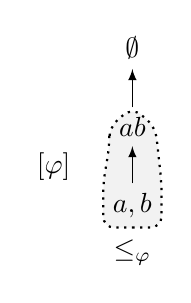
\begin{tikzpicture}
	\node at (0,-0.6){$\le_\phi$};
	\node at (0,0)(0){$a,b$};
	\node at (0,1)(1){$ab$};
	\node at (0,2)(2){$\emptyset$};
	\node at (-1, 0.5){$[\phi]$};
	\path[-latex] (0) edge (1)
	(1) edge (2);
	\fill[opacity=0.05, rounded corners=4pt]
		(0.south)--
		(0.south east)--
		(0.east)--
		(0.north east)--
		(1.east)--
		(1.north)--
		(1.west)--
		(1.south west)--
		(0.north west)--
		(0.west)--
		(0.south west)--
		(0.south);
	
	\draw[thick, dotted, rounded corners=4pt]
		(0.south)--
		(0.south east)--
		(0.east)--
		(0.north east)--
		(1.east)--
		(1.north)--
		(1.west)--
		(1.south west)--
		(0.north west)--
		(0.west)--
		(0.south west)--
		(0.south);
	\end{tikzpicture} 
	\caption{
		An agent with prior beliefs $\phi$, $[\phi]=\{a,b,ab\}$, 
		thinks outcomes $a$ and $b$ are more likely than $ab$.
		When revising by $\phi$, the result is $[\phi\re\phi]=\{a,b\}$,
		which does not fit with postulate $\ppr{\IAHB}$.
	}
	\label{fig:4-non-stability}
\end{figure}

\begin{xmpl}{Independence to already held beliefs}{4-non-iahb}
	For the set of atoms $\Atoms=\{a,b\}$,
	consider an agent whose prior beliefs are represented by the formula $\phi=a\lor b$,
	who revises according to a revision operator $\re$ that satisfies postulate $\ppr{9}$,
	and who ranks interpretations according to the total preorder $\le_\phi$ in Figure~\ref{fig:4-non-stability}.
	The agent finds out, on good authority, information consistent with $\phi$.
	On revising by $\phi$, the result is $[\phi\re\phi]=\min_{\le_\phi}[\mu] = \{a,b\}$,
	i.e., $\phi\re\phi\equiv (a\leftrightarrow\lnot b)$,
	and it is apparent that $\phi\re\phi\not\equiv\phi$ 
	and that postulate $\ppr{\IAHB}$ is not satisfied.
\end{xmpl}

In fact, postulate $\ppr{\IAHB}$ characterizes a property on interpretations
that coincides with neither of the properties introduced in this chapter,
but is familiar from Section \ref{sec:3-revision}:
recall, from there, property $\oor{5}$, saying that if two interpretations $w_1$ and $w_2$ 
are models of $\phi$, then $w_1\approx_\phi w_2$.

\begin{thm}{}{revision-representation-indifference}
	If an $\L$-revision operator $\re$ 
	satisfies postulates $\ppr{1}$ and $\ppr{3-6}$
	(i.e., is exhaustive)
	and $\as$ is a total $\L$-assignment on interpretations
	that represents it,
	then
	$\re$ satisfies postulate $\ppr{\IAHB}$ if and only if 
	$\as$ satisfies property $\oor{5}$.
\end{thm}
\begin{prf*}{}{}%
	(``$\Rightarrow$'')
	Consider an exhaustive revision operator $\re$ that satisfies postulates $\ppr{1}$ and $\ppr{3-6}$
	and, in addition, postulate $\ppr{\IAHB}$, 
	and an assignment $\as$ that represents it.
	Take two interpretations $v_1$ and $v_2$ such that $v_1,v_2\in[\phi]$. 
	Applying postulate $\ppr{\IAHB}$, it follows that $v_1,v_2\in[\phi\re\phi]$,
	and hence $v_1,v_2\in\min_{\le_\phi}[\phi]$, i.e., $v_1\approx_\phi v_2$.

	(``$\Leftarrow$'')
	Starting from an assignment $\as$ and the revision operator that represents it,
	assuming that $\oor{5}$ is satisfied, we have that $\min_{\le_\phi}[\phi] = [\phi]$,
	which implies that postulates $\ppr{\IAHB}$ is satisfied.
\end{prf*}

The ability to distinguish among models of one's prior beliefs
in terms of plausibility
points to a more graded view of what it means
to believe $\phi$. Thus, an agent might have a certain threshold of plausibility,
along the lines of what is known in epistemology
as \emph{the Lockean thesis}~\cite{Foley93},
according to which it calibrates its beliefs: 
anything above the threshold counts as part of the belief $\phi$
and anything below counts as disbelief.
This fits with the idea that an agent
might assign different degrees of plausibility to states of affairs
consistent with its belief $\phi$:
indeed, this is the point of view we endorse here,
in contrast to more standard approaches, which consider
that an agent assigns equal 
degrees of plausibility to all items of its belief.
Thus, incoming information that confirms an agent's belief might have the effect
of \emph{reinforcing} parts that are given more plausibility
at the expense of parts that are given less,
and this is the kind of situation we take to be
modeled by Example~\ref{ex:4-non-iahb}.

What would be worrying would be a revision policy
that makes an agent cycle between different viewpoints
when confronted repeatedly with the same type of information:
we will see that for revision operators satisfying $\ppr8$
this concern is unwarranted, but we must first introduce some new notation.
% If $\phi$ is a formula,
If $\phi$ is a propositional formula and $\re$ is a revision operator,
then $\phi^i$ is the formula obtained 
by revising $\phi$ by itself, using $\re$, an $i$ number of times.
Thus, $\phi^0=\phi$ and $\phi^{i+1}={\phi^i}\re{\phi}$.
Consider now the following property,
written as a postulate
meant to apply for any propositional formula $\phi$:

\begin{description}
	\item[($\ppr{\STAB}$)] There is $n\geq 1$ such that $\phi^m\equiv\phi^n$,	for every $m\geq n$.
\end{description}

Postulate $\ppr{\STAB}$, where `$\STAB$' stands for \emph{Stability},
implies that repeated revision by $\phi$ ultimately 
settles (or stabilizes) on a set of models
that does not change through subsequent revisions by $\phi$.
A revision operator $\re$ is \emph{stable} 
if it satisfies postulate $\ppr{\STAB}$. 
The following result proves relevant to the issue of stability.

\begin{prp}{}{4-inclusion-stability}
	If a revision operator $\re$ satisfies postulates $\ppr{1}$ and $\ppr{9}$,
	then $\phi^{i+1}\models\phi^i$.
\end{prp}
\begin{prf*}{}{}%
	By postulate $\ppr{1}$, we have that $\phi\re\phi\models\phi$,
	and thus $\phi^1\models\phi^0$.
	Applying postulate $\ppr{9}$,
	we have that $(\phi\re\phi)\re\phi\models(\phi\re\phi)\land\phi\models\phi\re\phi$.
	Thus, $\phi^2\models\phi^1$, and it is straightforward to see how this argument
	is iterated to get the conclusion.
\end{prf*}

If the operator $\re$ also satisfies postulate $\ppr{3}$ 
(i.e., if the revision formula
is consistent, then the revision result is also consistent),
it follows that if $\phi$ is consistent, 
then $\phi_i$ is consistent, for any $i\geq 0$.
Thus, combining this fact and Proposition \ref{prop:4-inclusion-stability},
we get that 
repeated revision by $\phi$ leads to a chain of ever more specific formulas,
i.e.,
$\emptyset\subset\dots\subseteq\mods{\phi^{i+1}}\subseteq\mods{\phi^i}\subseteq\dots\subseteq\mods{\phi^0}$.
Since a formula has a finite number of models, it falls out immediately
from this that there must be a point at which further revision by $\phi$
does not change anything.

\begin{crl}{}{stability}
	If a revision operator $\re$ satisfies postulates $\ppr{1}$ and $\ppr{8}$,
	then $\re$ is stable.
\end{crl}

Unfortunately, postulates $\ppr{11-12}$ do not guarantee stability.
Since these postulates require only that the agent places the models of $\dual{\phi}$
as the least plausible interpretations,
it becomes possible that an agent's plausibility
ranking does not hold on to a core set of interpretations
through successive revisions by $\phi$.

\begin{figure}\centering
	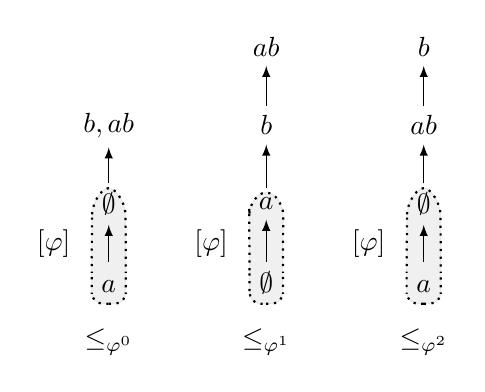
\begin{tikzpicture}
	\node at (0,-0.75){$\le_{\phi^0}$};
	\node at (0,0)(0){$a\vphantom{\emptyset}$};
	\node at (0,1)(1){$\emptyset$};
	\node at (0,2)(2){$b, ab$};
	\node at (-0.7, 0.5){$[\phi]$};
	\path[-latex] (0) edge (1)	(1) edge (2);
	\fill[draw, opacity=0.06, rounded corners=4pt]
		(0.south)--
		(0.south east)--
		(0.east)--
		(0.north east)--
		(1.east)--
		(1.north)--
		(1.west)--
		(1.south west)--
		(0.north west)--
		(0.west)--
		(0.south west)--
		(0.south);
	\draw[thick, dotted, rounded corners=4pt]
		(0.south)--
		(0.south east)--
		(0.east)--
		(0.north east)--
		(1.east)--
		(1.north)--
		(1.west)--
		(1.south west)--
		(0.north west)--
		(0.west)--
		(0.south west)--
		(0.south);
	
	\node at (2,-0.75){$\le_{\phi^1}$};
	\node at (2,0)(01){$\emptyset$};
	\node at (2,1)(11){$a$};
	\node at (2,2)(21){$b$};
	\node at (2,3)(31){$ab$};
	\node at (1.3, 0.5){$[\phi]$};
	\path[-latex] (01) edge (11)(11) edge (21)(21) edge (31);
	\fill[draw, opacity=0.06, rounded corners=4pt]
		(01.south)--
		(01.south east)--
		(01.east)--
		(01.north east)--
		(11.east)--
		(11.north)--
		(11.west)--
		(11.south west)--
		(01.north west)--
		(01.west)--
		(01.south west)--
		(01.south);
	\draw[thick, dotted, rounded corners=4pt]
		(01.south)--
		(01.south east)--
		(01.east)--
		(01.north east)--
		(11.east)--
		(11.north)--
		(11.west)--
		(11.south west)--
		(01.north west)--
		(01.west)--
		(01.south west)--
		(01.south);
	
	\node at (4,-0.75){$\le_{\phi^2}$};
	\node at (4,0)(02){$a\vphantom{\emptyset}$};
	\node at (4,1)(12){$\emptyset$};
	\node at (4,2)(22){$ab$};
	\node at (4,3)(32){$b$};
	\node at (3.3, 0.5){$[\phi]$};
	\path[-latex] (02) edge (12)(12) edge (22)(22) edge (32);
	\fill[draw, opacity=0.06, rounded corners=4pt]
		(02.south)--
		(02.south east)--
		(02.east)--
		(02.north east)--
		(12.east)--
		(12.north)--
		(12.west)--
		(12.south west)--
		(02.north west)--
		(02.west)--
		(02.south west)--
		(02.south);
	\draw[thick, dotted, rounded corners=4pt]
		(02.south)--
		(02.south east)--
		(02.east)--
		(02.north east)--
		(12.east)--
		(12.north)--
		(12.west)--
		(12.south west)--
		(02.north west)--
		(02.west)--
		(02.south west)--
		(02.south);
	\end{tikzpicture} 
	\caption{
		For an agent with prior information $\phi$, $[\phi]=\{\emptyset,a\}$,
		repeated revision by $\phi$ cycles between $\set{a}$ and $\set{\emptyset}$. 
	}
	\label{fig:postulates-89-not-stable}
\end{figure}


\begin{xmpl}{Stability}{postulates89-not-stable}
	For the set of atoms $\Atoms=\{a,b\}$
	consider an agent whose prior information is represented by the formula
	$\phi=\lnot b$,
	revises their beliefs with an operator $\re$ that satisfies postulates $\ppr{11-12}$,
	and who ranks outcomes as shown in Figure~\ref{fig:postulates-89-not-stable}.
	We have that $[\phi^0]=[\phi]=\{\emptyset,a\}$,
	$[\phi^1]=[\phi\re\phi]=\{a\}$,
	and $[\phi^2]=[\phi^1\re\phi]=\{\emptyset\}$.
	%By postulate~\R{3}, %we get that 
	By postulate $\ppr{4}$, we infer that subsequent revisions by $\phi$
	cycle between $\{a\}$ and $\{\emptyset\}$,
	i.e., 
	$[\phi^3]=\{a\}$,
	$[\phi^4]=\{\emptyset\}$,
	and so on, 
	therefore 
	thus never settling on a stable answer.
\end{xmpl}

The issue of stability suggests another dimension along which
revision operators can be analyzed, with Corollary~\ref{cor:stability}
and Example~\ref{ex:postulates89-not-stable} showing that a revision operator does not 
satisfy it trivially. 
Example~\ref{ex:postulates89-not-stable}, in particular, shows that there is 
interplay between $\le_\phi$ and $\le_{\phi'}$, if $\phi'\models\phi$,
which is relevant to the question of whether an operator is stable.
This interplay is reminiscent of topics like iterated 
revision and kinetic consistency~\cite{DarwicheP97,PeppasW16},
but pursuing it further would take us too far afield of the aims of the current work.


%%%%%%%%%%%%%%%%%%%%%%%%%%%%%%%%%%%%%%%%%%%%%%%%%%%%%%%%%%%%%%%%%%%%%%%%%%%%%%%%%%%%%%%%%%%%%%%%%%%%%%%%%%%%%%%

\section{Distance-based biased revision operators}\label{sec:4-dist-based-biased operators}
Having characterized revision operators in terms of 
assignments on interpretations, we now ask: 
what is a natural way to construct operators with such biases?
We will use the insight afforded by Theorem \ref{thm:4-biased-revision-repr}
to generate rankings on outcomes
that reflect the design principles outlined by postulates $\ppr{9-13}$.
In the process, we employ the two familiar ingredients from Section \ref{sec:2-distances}.
The first is a quasi-distance $\dd$ between interpretations,
interpreted as a measure of plausibility 
of one interpretation relative to the other.
The second ingredient is an aggregation function $\agg$,
used to compare interpretations given the distances generated by $\dd$.
Putting these two ingredients together,
we have a total $(\dd,\:\agg)$-induced $\L$-assignment $\as^{\dd,\:\agg}_\phi$,
which in turn induces the revision operator $\re^{\dd,\:\agg}$.

For quasi-distances, we will use drastic distance $\dd_\drastic$ and Hamming distance $\dd_\hamming$.
For aggregation functions, we use the ones introduced in Section \ref{sec:2-distances}, 
plus two new ones that we introduce in the following.
The \textit{$\dd$-centrality $\dd^\ctr(\phi,w)$ of $w$ with respect to $\phi$}
is defined as $\dd^\ctr(\phi, w)=\dd^\max(\phi,w)-\dd^\min(\phi, w)$.
The \emph{$\dd$-displacement $\dd^\dis(\phi,w)$ of $w$ with respect to $\phi$}
is $\dd^\dis(\phi,w)=\dd^\min(\phi,w)-\dd^\min(w^\ast,\phi)$,
where $w^\ast$ is an interpretation
such that $\dd^\min(w^\ast,\phi)$ is minimal among all
the interpretations $w'$ for which $\dd^\ctr(w',\phi)=\dd^\ctr(\phi,w)$.
Finally, 
the \textit{$\dd$-agreeability $\dd^\agr(\phi,w)$ of $w$ with respect to $\phi$} is  
defined as
$\dd^\agr(\phi,w)=\min\{\dd^\min(\phi,w),~\dd^\ctr(\phi,w)+\dd^\dis(\phi,w)\}$,
while the \textit{$\dd$-disagreeability $\dd^\dagr(\phi,w)$ of $w$ with respect to $\phi$}
is defined as 
%$\dagr(\phi,w)=\min\set{\min\dd{w,\dual{\phi}},~ 
%\ctr{w,\dual{\phi}}+\dis{w,\dual{\phi}}}$,
$\dd^\dagr(\phi,w)=m-\dd^\agr(\dual{\phi},w)$, where $m=|\Atoms|$.

\begin{xmpl}{Aggregation functions}{comparison-function}
	Take the formula $\phi=(b\rightarrow a)$, with 
	$[\phi]=\{\emptyset,a,ab\}$,
	and the interpretation $w=\emptyset$.
	The vector of Hamming distances from every model of $\phi$ to $w$ is:	
	$$
		(\dd_\hamming(\emptyset,\emptyset), \dd_\hamming(a,\emptyset),\dd_\hamming(ab,\emptyset)) = (0,1,2).
	$$
	We obtain that 
	$\dd_\hamming^\leximax(\phi,w)=(2,1,0)$
	and 
	$\dd_\hamming^\leximin(\phi,w)=(0,1,2)$.
	Additionally, we have that:
	\begin{align*}
		\dd^\min_\hamming(\phi,w)   & = 0,\\
		\dd^\max_\hamming(\phi,w)   & = 2,\\
		\dd^\ssum_\hamming(\phi, w) & = 0+1+2 = 3,\\
		\dd^\ctr_\hamming(\phi,w)   & = 2-0 = 2,\\
		\dd^\agr_\hamming(\phi, w)  & = (2-0) \cdot 0 = 0.
	\end{align*}
\end{xmpl}

Notice that the centrality of $w$ with respect to $\phi$ is $0$	
just in case $\dd^\min(\phi,w)=\dd^\max(\phi,w)$,
i.e., just in case $w$ is at equal distance to every model of $\phi$.
Thus, the agreeability index of $w$ with respect to $\phi$ is $0$
just in case $w$ is either a model of $\phi$,
or equally distanced to every model of $\phi$.

Putting these ingredients together gives us the revision operators
$\re^{\dd,\:\min}$,
$\re^{\dd,\:\leximin}$,
$\re^{\dd,\:\max}$,
$\re^{\dd,\:\leximax}$,
$\re^{\dd,\:\ssum}$,
$\re^{\dd,\:\agr}$,
$\re^{\dd,\:\dagr}$,
for $\dd\in\{\dd_\hamming,\dd_\drastic\}$.
Out of these, $\re^{\hamming,\:\min}$ is the Dalal operator
and $\re^{\drastic,\:\min}$ is the drastic operator,
presented in Section \ref{sec:3-revision}.
Thus, this perspective manages to capture 
known operators, while paving the way for some new ones.

The best way to understand these operators is to see how they rank interpretations in the universe.

\begin{table}\centering
\begin{tabular}{lccccccccc}
	%&\multicolumn{4}{c}{$[\phi]$}&&&&&\\
	\toprule
										&
	$\emptyset$ 						&
	$a$ 								& 
	$b$ 								& 
	$abc$								& 
	$\leximin$ 							& 
	$\leximax$ 							&
	$\min$								&
	$\max$								& 
	$\ssum$								\\\midrule

	$\emptyset$ 						& 
	$0$									&
	$1$									& 
	$1$									& 
	$3$									& 
	$(0,1,1,3)$							&
	$(3,1,1,0)$							&
	$0$									&	
	$3$									& 
	$5$									\\
	
	$a$									& 
	$1$									& 
	$0$									& 
	$2$									& 
	$2$									& 
	$(0,1,2,2)$							&
	$(2,2,1,0)$							&
	$0$									&
	$2$									& 
	$5$									\\

	$b$									& 
	$1$									& 
	$2$									& 
	$0$									& 
	$2$									& 
	$(0,1,2,2)$							&
	$(2,2,1,0)$							&
	$0$									&
	$2$									& 
	$5$									\\

	$c$									& 
	$1$									& 
	$2$									& 
	$2$									& 
	$2$									& 
	$(1,2,2,2)$							&
	$(2,2,2,1)$							&
	$1$									&
	$2$									& 
	$7$									\\

	$ab$								& 
	$2$									&
	$1$									& 
	$1$									& 
	$1$									& 
	$(1,1,1,2)$							&
	$(2,1,1,1)$							&
	$1$									&
	$2$									& 
	$5$									\\
	
	$ac$								& 
	$2$									&
	$1$									& 
	$3$									& 
	$1$									& 
	$(1,1,2,3)$							&
	$(3,2,1,1)$							&
	$1$									&
	$3$									&
	$7$									\\
	
	$bc$								& 
	$2$									&
	$3$									& 
	$1$									& 
	$1$									& 
	$(1,1,2,3)$							&
	$(3,2,1,1)$							&	
	$1$									&
	$3$									& 
	$7$									\\
	
	$abc$								& 
	$3$									&
	$2$									& 
	$2$									& 
	$0$									& 
	$(0,2,2,3)$							&
	$(3,2,2,0)$							&
	$0$									&
	$3$									& 
	$7$									\\\bottomrule
\end{tabular}
\caption{
	The table of Hamming distances from the models of 
	$\phi$, with $[\phi]=\{\emptyset,a,b,abc\}$,
	to every interpretation in a universe generated from three atoms.
	The aggregated values according to the aggregation functions presented in this chapter
	are also displayed.
}
\label{table:distances-example}
\end{table}


\begin{xmpl}{Distance-based biased preorders}{ops-example1}
	For the set of atoms $\Atoms=\{a,b,c\}$,
	take $\phi=(\lnot(a\land b)\land\lnot c)\lor (a\land b\land c)$,
	for which it holds that $[\phi]=\{\emptyset,a,b,abc\}$.
	For the interpretation $w=\emptyset$,
	we have that 
	$\dd^\leximin_\hamming(\phi,w)=(0,1,1,3)$,
	$\dd^\leximax_\hamming(\phi,w)=(3,1,1,0)$,
	$\dd^\min_\hamming(\phi,w)=0$,
	$\dd^\max_\hamming(\phi,w)=3$ and
	$\dd^\ssum_\hamming(\phi,w)=5$.
	The distances and aggregated distances for each
	interpretation are depicted in Table~\ref{table:distances-example}.
	Notice how the models of $\phi$
	are distributed when the interpretations are ranked according
	to the different aggregation functions used:
	we have $\emptyset\approx^{\hamming,\:\min}_\phi a$,
	since $\dd^\min_\hamming(\phi,\emptyset)=\dd^\min_\hamming(\phi,a)=0$,
	but $\emptyset<_\phi^{\hamming,\:\leximin} a$,
	since $(0,1,1,3)<_\lex(0,1,2,2)$.
	Also, we have that $c<_\phi^{\hamming,\:\max}abc$,
	$c<_\phi^{\hamming,\:\leximax}abc$
	and $ab<_\phi^{\hamming,\:\ssum}abc$, i.e.,
	models of $\phi$ are not minimal in $\le_\phi^{\hamming,\:\max}$,
	$\le_\phi^{\hamming,\:\leximax}$ and $\le_\phi^{\hamming,\:\ssum}$.
	In particular, $\le_\phi^{\hamming,\:\max}$ makes the models of $\dual{\phi}$
	(i.e., $abc$, $bc$, $ac$ and $\emptyset$)
	the least plausible interpretations. 	
\end{xmpl}

The agreement and disagreement operators 
($\re^{\dd,\:\agr}$ and $\re^{\dd,\:\dagr}$)
are simpler than they appear:
the idea behind $\re^{\dd,\:\agr}$ is to allow
interpretations other than the models of $\phi$
as the minimal elements of the preorder $\le_\phi$.
Notice that the score of an interpretation in $\le_\phi^{\dd,\:\agr}$
is $0$ if it is either a model of $\phi$,
or it is equidistant from every model of $\phi$
(i.e., its centrality is $0$) and it is the `closest'
interpretation to $\phi$ with this property. 
The disagreement operator $\re^{\dd,\:\dagr}$ works in similar fashion,
by making models of $\dual{\phi}$ and interpretations minimally equidistant to them 
the least plausible interpretations in $\le_\phi^{\dd,\:\dagr}$.

\begin{xmpl}{Agreement and disagreement operators}{ops-example2}
	If $\Atoms=\{a,b,c\}$,
	take $\phi$ such that $[\phi]=\{a,b,c\}$,
	and notice that $\emptyset$ and $abc$ 
	are both equidistant to $\phi$,
	hence their centrality is $0$.
	However, $\emptyset$ is closer to $\phi$ than $abc$
	(its displacement is $0$, compared to $abc$'s displacement of $1$),
	and $\dd_\hamming^\agr(\phi,\emptyset)=0$.
	Thus, what $\dd_\hamming^\agr$ does is to give
	a minimal score to models of $\phi$ and to the minimally equidistant
	interpretation $\emptyset$.
	By contrast, $\dd_\hamming^\dagr$ gives a maximal score
	to the models of $\dual{\phi}$ and to the maximally equidistant 
	interpretation $abc$.
\end{xmpl}

All operators proposed generate a total preorder 
$\le^{\dd,\:\agg}_\phi$ over interpretations, 
but differ in how they arrange 
models of $\phi$:
this corresponds to the different attitudes an agent can have towards
$\phi$ prior to any revision.
The operator $\re^{\hamming,\:\min}$,
known as Dalal's operator~\cite{Dalal88},
considers all models of $\phi$
as the most plausible elements in $\le_\phi^{\hamming,\:\min}$
and is the only operator of the ones considered here
for which $\phi\re\mu$ is equivalent to $\phi\land\mu$
when $\phi\land\mu$ is consistent.
%This operator is Dalal's operator~\cite{DBLP:conf/aaai/Dalal88}, and corresponds to the standard type of operator one finds in the literature.
Similarly, $\re^{\hamming,\:\leximin}$ %[{\bf SW} Check!],
also ranks models of $\phi$ as more plausible than any other interpretation,
but discriminates among models of $\phi$
% now are considered more plausible than others,
according to how typical, or representative they are 
of the general point of view expressed by $\phi$.
The operators 
$\le_\phi^{\hamming,\:\max}$
and $\le_\phi^{\hamming,\:\leximax}$
push away models of $\dual{\phi}$,
under the assumption that they are the most implausible possible worlds.
They difference between them is that $\le_\phi^{\hamming,\:\max}$ considers models of $\dual{\phi}$ equally implausible,
whereas $\le_\phi^{\hamming,\:\leximax}$ uses the more fine-grained lexicographic approach.
The operator $\re^{\hamming,\:\agr}$ 
makes models of $\phi$ the most plausible elements in $\le_\phi$ but 
does not stop here and 
also allows other interpretations on that position,
in particular certain interpretations that are equidistant to $\phi$
as per Example \ref{ex:ops-example2}.
Specifically, an interpretation can be on the lowest level of $\le_\phi$
if it either is a model of $\phi$, or is at equal distance to every model of $\phi$.
The intuition is that an interpretation equally distanced from models of $\phi$ is 
%something 
like a compromise point of view, 
with good chances of being correct if it is close to $\phi$.
The operator $\re^{\hamming,\:\dagr}$ is the dual of 
$\re^{\hamming,\:\agr}$ and,
finally, operator $\re^{\hamming,\:\ssum}$ evokes
utilitarian approaches
by choosing interpretations
that minimize the sum of the distances to each model of $\phi$,
i.e., are close to $\phi$ on an aggregate level.

Plugging in the drastic and Hamming distances  
would seem to give us a considerable number of operators,
but quick reflection shows that operators
obtained with drastic distance $\dd_\drastic$ collapse into two main categories.
%To get an idea of what these categories are,
%consider the following two types of revision operators,
%defined syntactically for a change.
To get a grasp on this fact, 
consider first the \textit{drastic revision operator $\re^\drastic$} defined,
for any propositional formulas $\phi$ and $\mu$,
as
$\phi\re^\drastic\mu=\phi\land\mu$, if $\phi\land\mu$ is consistent, and $\mu$ otherwise,
and the \textit{forgetful revision operator $\re^\forgetful$} defined as
%is defined, for $\phi\in\L_\cn$ 
%and $\mu\in\L$,
$\phi\re^\forgetful\mu=\mu$.
It is forgetful because it disregards initially held beliefs completely,
always adopting the new information $\mu$.

\begin{prp}{}{4-br-drastic-dist-ops}
	For any propositional formulas $\phi$ and $\mu$,
	it holds that 
	$\phi\re^{\drastic,\:\min}\mu
	\equiv
	\phi\re^{\drastic,\:\leximin}\mu
	\equiv
	\phi\re^{\drastic,\:\leximax}\mu
	\equiv
	\phi\re^{\drastic,\:\ssum}\mu
	\equiv
	\phi\re^\drastic\mu$.
	Moreover, $\phi\re^{\drastic,\:\agr}\mu\equiv\phi\re^\forgetful\mu$ and
	$\phi\re^{\drastic,\:\max}\mu\equiv\phi\re^{\drastic,\:\dagr}\mu\equiv
	\begin{cases}
	\phi\re^\drastic\mu,~\text{if}~\phi~\text{is complete},\\
	\phi\re^\forgetful\mu,~\text{otherwise}.
	\end{cases}
	$
\end{prp}
\begin{prf*}{}{}%
	If $\phi$ is a complete formula
	such that $[\phi]=\{v\}$,
	then 
	$\dd^\agg_\drastic(\phi,w)=\dd_\drastic(v,w)$,
	for all aggregation functions $\agg\in\{\min,\max,\leximin,\leximax,\ssum,\agr,\dagr\}$,
	and any interpretation $w$.
	In other words, it holds that:
	$$
	\dd^\agg_\drastic(\phi,w)=
		\begin{cases}
		0,~\text{if}~w=v,\\
		1,~\text{otherwise}.
		\end{cases}
	$$ 
	It is thus straightforward to conclude that if $v\in[\mu]$,
	then $[\phi\re^{\drastic,\:\max}\mu]=\{v\}=[\phi\land\mu]$,
	and if $w_0\notin[\mu]$,
	then $[\phi\re^{\drastic,\:\max}\mu]=[\mu]$.
	If $\phi$ is not complete, then we have that:
	$$
	\dd^\leximin_\drastic(\phi,w)=
		\begin{cases}
		(0,1,\dots,1),~\text{if}~w\in[\phi],\\
		(1,1,\dots,1),~\text{otherwise}.
		\end{cases}
	$$
	It is now straightforward to see that the remaining
	statements of Proposition~\ref{prop:4-br-drastic-dist-ops} hold.
\end{prf*}

We can illustrate the differential treatment of operator $\re^{\drastic,\:\max}$ 
through an example.

\begin{figure}\centering
	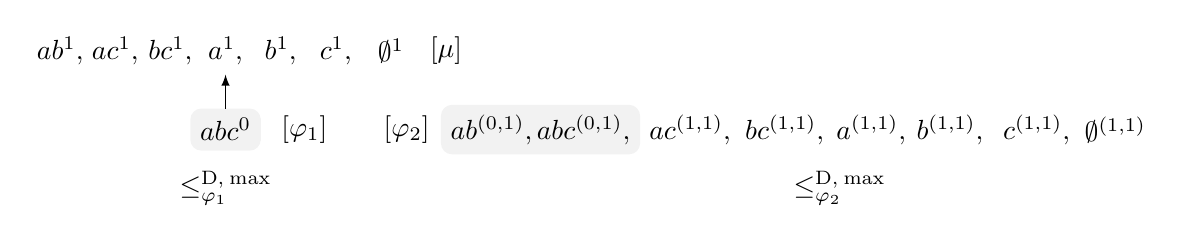
\begin{tikzpicture}			
		\node at (1, 0) {$\mods{\phi_1}$};
		\node at (2.8, 1) {$[\mu]$};
		
		\node at (0,-0.75){$\le_{\phi_1}^{\drastic,\:\max}$};
		\node at (0,0) (abc) {$abc^{{0}}$};
		\node at (-2.1, 1) (ab){$ab^{{1}},$};
		\node at (-1.4,1) (ac){$ac^{{1}},$};
		\node at (-0.7, 1) (bc){$bc^{{1}},$};
		\node at (0, 1) (a){$a^{{1}},$};
		\node at (0.7, 1) (b){$b^{{1}},$};
		\node at (1.4, 1) (c){$c^{{1}},$};
		\node at (2.1, 1) (e){$\emptyset^{{1}}$};
		
		\path[-latex] (abc) edge (a);
		\fill[opacity = 0.05, rounded corners=4]
			(abc.south) --
			(abc.south east) --
			(abc.east) --
			(abc.north east) --
			(abc.north) --
			(abc.north west) --
			(abc.west) --
			(abc.south west) --
			(abc.south);
		% \draw[thick, dotted, rounded corners=4]
		% 	(a.south)--
		% 	(b.south)--
		% 	(e.south)--
		% 	(e.south east)--
		% 	(e.east)--
		% 	(e.north east)--
		% 	(e.north)--
		% 	(e.north west)--
		% 	(c.south east)--
		% 	(c.south west)--
		% 	(b.north east)--
		% 	(b.north)--
		% 	(a.north)--
		% 	(a.north west)--
		% 	(a.west)--
		% 	(a.south west)--
		% 	(a.south);

		% \node at (-2, 0) {$\mods{\phi_2}$};
		% \node at (6.2, 0) {$[\mu]$};
%			\node at (0, 0.5){};
		
		\node at (2.3,0){$[\phi_2]$};
		\node at (7.8,-0.75){$\le_{\phi_2}^{\drastic,\:\max}$};
		\node at (4,0) (abc) {$ab^{(0,1)},abc^{(0,1)},$};
%			\node at (-2.4, 1) (ab){$ab^{{1}}$};
%			\node at (-1.6,1) (ac){$ac^{{1}}$};
		\node at (5.9, 0) (bc){$ac^{(1,1)},$};
		\node at (7.1, 0) (bc){$bc^{(1,1)},$};
		\node at (8.2, 0) (a){$a^{(1,1)},$};
		\node at (9.2, 0) (b){$b^{(1,1)},$};
		\node at (10.3, 0) (c){$c^{(1,1)},$};
		\node at (11.3, 0) (e){$\emptyset^{(1,1)}$};
		
		\fill[opacity = 0.05, rounded corners=4]
			(abc.south) --
			(abc.south east) --
			(abc.east) --
			(abc.north east) --
			(abc.north) --
			(abc.north west) --
			(abc.west) --
			(abc.south west) --
			(abc.south);
		% \draw[thick, dotted, rounded corners=4]
		% 	(a.south)--
		% 	(b.south)--
		% 	(e.south)--
		% 	(e.south east)--
		% 	(e.east)--
		% 	(e.north east)--
		% 	(e.north)--
		% 	(e.north west)--
		% 	(c.south east)--
		% 	(c.south west)--
		% 	(b.north east)--
		% 	(b.north)--
		% 	(a.north)--
		% 	(a.north west)--
		% 	(a.west)--
		% 	(a.south west)--
		% 	(a.south);
		\end{tikzpicture}                
		\caption{
			Preorders $\le^{\drastic,\:\max}_{\phi_1}$ and $\le^{\drastic,\:\max}_{\phi_2}$,
			for $\mods{\phi_1}=\set{abc}$ and $\mods{\phi_2}=\set{ab, ac, abc}$.
			Depicted as superscript to an interpretation $w$ is the vector of drastic distances $\dd_\drastic$ 
			from the models of $\phi_1$ and $\phi_2$, respectively, to $w$.
			Since $\phi_1$ is complete (i.e., has only one model), this vector consists of only one number.
			The $\max$ aggregation function uses the maximum value in the vector of distances to compare interpretations.
			}
	\label{fig:4-br-drastic-max}
\end{figure}

\begin{xmpl}{Drastic operators}{4-br-drastic-max}
	For the set of atoms $\Atoms=\{a,b,c\}$,
	consider the complete formula 
	$\phi_1 = \{a\land b\land c\}$.
	We have that:
	\begin{align*}
		\dd^\max_\drastic(\phi,w) &=\dd_\drastic(abc,w)\\
									&=\begin{cases}
										0,~\text{if}~w=abc,\\
										1,~\text{otherwise}.
									\end{cases}
	\end{align*}
	The preorder $\le_{\phi_1}^{\drastic,\:\max}$ is depicted on the left in
	Figure \ref{fig:4-br-drastic-max}.
	Consider, then, a formula
	$\phi_2 = a\land b$,
	with $[\phi_2]=\{ab, abc\}$.
	In this case we obtain, for instance, that
	$\dd^\max_\drastic(\phi,w)$, for every interpretation $w$ in the universe.
	The preorder $\le_{\phi_2}^{\drastic,\:\max}$ is depicted on the right in
	Figure~\ref{fig:4-br-drastic-max},
	which illustrates the fact that in this case $\re^{\drastic,\:\max}$ is equivalent to 
	the forgetful operator $\re^\forgetful$.
\end{xmpl}

With Hamming distance
the landscape is more diverse,
as the different attitudes the operators
assume towards models of $\phi$ lead to genuinely different
revision strategies.
Nonetheless,
certain relationships between the operators still hold, with
lexicographic operators being the most
discriminating, in the sense that they pick
formulas with fewer models, i.e., more specific formulas.
%We can get a better idea of how these operators work by looking at an example.

\begin{prp}{}{4-revision-operators-interrelations}
	If $\phi$ and $\mu$ are propositional formulas and $\dd$ is a quasi-distance,
	it holds that:
		\begin{description}
			\item[($a$)] $\phi\re^{\dd,\:\leximin}\mu\models\phi\re^{\dd,\:\min}\mu\models\phi\re^{\dd,\:\agr}\mu$,
			\item[($b$)] $\phi\re^{\dd,\:\leximax}\mu\models\phi\re^{\dd,\:\max}\mu\models\phi\re^{\dd,\:\dagr}\mu$.
		\end{description}
\end{prp}


%\begin{example}
%Take a formula $\phi$
%such that $[\phi]=\set{\emptyset,ad, abde, abcehg}$
%and a formula $\mu$ such that $[\mu]=\set{a,ab, abc,abcd,abde,abcehg}$.
%All the distances,
%together with the selection functions applied to them,
%are depicted in Table~\ref{table:table-of-distances}.
%For the preorders generated by these distances, see 
%Figures~\ref{fig:hamming-min-max}, 
%\ref{fig:hamming-leximin-leximax} 
%and \ref{fig:hamming-agre-summing}.
%
%\begin{table*}[t]\centering
%\begin{tabular}{l cccc cccccc}
%\toprule
%& 
%$\emptyset$ & 
%$ad$ & 
%$abde$ & 
%$abcehg$ & 
%$\ascending{\dd_\hamming(\phi,w)}$ &
%$\dd^\leximin_\hamming(\phi,w)$ &
%$\min$ &
%$\max$ &
%$\agr$ & 
%$\sum$\\\midrule
%$\emptyset$ & 0 & 2 & 4 & 6 &${0246}$ & ${6420}$& 0 & 6& 0& 12\\
%$ad$ & 2 & 0 & 2 & 6 &${0226}$& ${6220}$& 0 & 6 & 0& 10\\
%$abde$ & 4 & 2 & 0 & 4 &${0244}$& ${4420}$& 0 & 4 & 0 &10\\
%$abcehg$ & 6 & 6 & 4 & 0 &${0466}$& ${6640}$& 0 & 6 & 0 &16\\
%$a$ & 1 & 1 & 3 & 5 &${1135}$& ${5311}$& 1 & 5 & 4& 10\\
%$ab$ & 2 & 2 & 2 & 4 &${2224}$& ${4222}$ & 2 & 4 & 4 & 10\\
%$abc$ & 3 & 3 & 3 & 3 &${3333}$& ${3333}$& 3 & 3 & 0& 12\\
%$abcd$ & 4 & 2 & 2 & 4 &${2244}$& ${4422}$& 2 & 4 & 4& 12\\\bottomrule
%\end{tabular}
%\caption{Distances $\dd_\hamming(\phi,w)$ and the aggregation functions}
%\label{table:table-of-distances}
%\end{table*}
%%\begin{figure}\centering
%%	\begin{subfigure}[b]{0.45\textwidth}\centering
%%		\begin{tikzpicture}
%%		\node at (2.3,0)(k){$[\phi]$};
%%		\node at (1.5,2)(mu){$[\mu]$};
%%		\node at (-1.5,0) (e){$\emptyset^0$};
%%		\node at (-0.8,0) (ad){$ad^0$};
%%		\node at (0,0) (abde){$abde^0$};
%%		\node at (1.2,0) (abcehg){$abcehg^0$};
%%		\node at (0,1) (a){$a^1$};
%%		\node at (-0.5,2) (ab){$ab^2$};
%%		\node at (0,3) (abc){$abc^3$};
%%		\node at (0.5,2) (abcd){$abcd^2$};
%%		
%%		\node at (0,0.2)(1){};
%%		\node at (0,0.8)(2){};
%%		\node at (0,1.2)(3){};
%%		\node at (0,1.8)(4){};
%%		\node at (0,2.2)(5){};
%%		\node at (0,2.8)(6){};	
%%		
%%		\path
%%		(1) edge (2)
%%		(3) edge (4)
%%		(5) edge (6);
%%		
%%		\fill[fill=opacity=0.2, rounded corners=4]
%%		(e.south)--
%%		(ad.south)--
%%		(abde.south)--
%%		(abcehg.south)--
%%		(abcehg.south east)--
%%		(abcehg.east)--
%%		(abcehg.north east)--
%%		(abcehg.north)--
%%		(abde.north)--
%%		(ad.north)--
%%		(e.north)--
%%		(e.north west)--
%%		(e.west)--
%%		(e.south west)--
%%		(e.south);
%%		\fill[fill=opacity=0.5, rounded corners=4]
%%		(abcehg.south)--
%%		(abcehg.south east)--
%%		(abcehg.east)--
%%		(abcehg.north east)--
%%		(abcehg.north)--
%%		(abde.north east)--
%%		(a.south east)--
%%		(a.east)--
%%		(abcd.east)--
%%		(abc.east)--
%%		(abc.north east)--
%%		(abc.north)--
%%		(abc.north west)--
%%		(abc.west)--
%%		(ab.west)--
%%		(a.west)--
%%		(abde.west)--
%%		(abde.south west)--
%%		(abde.south)--
%%		(abcehg.south);
%%		\end{tikzpicture}   
%%		\caption{$\le_\phi^\hamming{\min}$}                 
%%	\end{subfigure}
%%	\begin{subfigure}[b]{0.45\textwidth}\centering
%%		\begin{tikzpicture}
%%		\node at (2,2.3)(k){$[\phi]$};
%%		\node at (-2,4)(k){$\mods{\dual{\phi}}$};
%%		\node at (-2,1)(mu){$[\mu]$};
%%		
%%		\node at (-1,3) (e){$\emptyset^6$};
%%		\node at (-0.2,3) (ad){$ad^6$};
%%		\node at (1,1) (abde){$abde^4$};
%%		\node at (1,3) (abcehg){$abcehg^0$};
%%		\node at (0,2) (a){$a^5$};
%%		\node at (-1,1) (ab){$ab^4$};
%%		\node at (0,0) (abc){$abc^3$};
%%		\node at (0,1) (abcd){$abcd^4$};
%%		\node at (-1.5,4)(d){$d^7$};
%%		\node at (-0.9,4)(chg){$chg^7$};
%%		\node at (0.1,4)(bcehg){$bcehg^7$};
%%		\node at (1.5,4)(abcdehg){$abcdehg^7$};
%%		
%%		\node at (0,0.2)(1){};
%%		\node at (0,0.8)(2){};
%%		\node at (0,1.2)(3){};
%%		\node at (0,1.8)(4){};
%%		\node at (0,2.2)(5){};
%%		\node at (0,2.8)(6){};	
%%		\node at (0,3.2)(7){};	
%%		\node at (0,3.8)(8){};	
%%		
%%		\path
%%		(1) edge (2)
%%		(3) edge (4)
%%		(5) edge (6)
%%		(7) edge (8);
%%		
%%		\fill[fill=opacity=0.2,rounded corners=5]
%%		(e.south)--
%%		(ad.south)--
%%		(abcehg.south)--
%%		(abde.north)--
%%		(abde.north west)--
%%		(abde.west)--
%%		(abde.south west)--
%%		(abde.south)--
%%		(abde.south east)--
%%		(abde.east)--
%%		(abde.north east)--
%%		(abcehg.south east)--
%%		(abcehg.east)--
%%		(abcehg.north east)--
%%		(abcehg.north)--
%%		(ad.north)--
%%		(e.north)--
%%		(e.north west)--
%%		(e.west)--
%%		(e.south west)--
%%		(e.south);	
%%		\fill[fill=opacity=0.5, rounded corners=5]
%%		(abcehg.north)--
%%		(abcehg.north east)--
%%		(abcehg.east)--
%%		(abcehg.south east)--
%%		(a.north east)--
%%		(a.east)--
%%		(a.south east)--
%%		(abde.north east)--
%%		(abde.east)--
%%		(abde.south east)--
%%		(abc.east)--
%%		(abc.south east)--
%%		(abc.south)--
%%		(abc.south west)--
%%		(abc.west)--
%%		(ab.south west)--
%%		(ab.west)--
%%		(ab.north west)--
%%		(a.south west)--
%%		(a.west)--
%%		(a.north west)--
%%		(abcehg.south west)--
%%		(abcehg.west)--
%%		(abcehg.north west)--
%%		(abcehg.north);
%%		
%%		\fill[fill=spanishCrimson, opacity=0.3, rounded corners=5]
%%		(d.north)--
%%		(chg.north)--
%%		(bcehg.north)--
%%		(abcdehg.north)--
%%		(abcdehg.north east)--
%%		(abcdehg.east)--
%%		(abcdehg.south east)--
%%		(abcdehg.south)--
%%		(bcehg.south)--
%%		(chg.south)--
%%		(d.south)--
%%		(d.south west)--
%%		(d.west)--
%%		(d.north west)--
%%		(d.north);
%%		\end{tikzpicture}   
%%		\caption{$\le_\phi^\hamming{\max}$}                 
%%	\end{subfigure}
%%	\caption{
%%		Preorders generated with $\min$ and $\max$
%%	}
%%	\label{fig:hamming-min-max}
%%\end{figure}
%%
%%\begin{figure}\centering
%%	\begin{subfigure}[b]{0.45\textwidth}\centering
%%		\begin{tikzpicture}
%%		\node at (1,0)(k){$[\phi]$};
%%		\node at (1,5)(mu){$[\mu]$};
%%		
%%		\node at (0,2) (e){$\emptyset^{{0246}}$};
%%		\node at (0,0) (ad){$ad^{{0226}}$};
%%		\node at (0,1) (abde){$abde^{{0244}}$};
%%		\node at (0,3) (abcehg){$abcehg^{{0466}}$};
%%		\node at (0,4) (a){$a^{{1135}}$};
%%		\node at (0,5) (ab){$ab^{{2224}}$};
%%		\node at (0,7) (abc){$abc^{{3333}}$};
%%		\node at (0,6) (abcd){$abcd^{{2244}}$};
%%		
%%		\node at (0,0.2)(1){};
%%		\node at (0,0.8)(2){};
%%		\node at (0,1.2)(3){};
%%		\node at (0,1.8)(4){};
%%		\node at (0,2.2)(5){};
%%		\node at (0,2.8)(6){};	
%%		\node at (0,3.2)(7){};
%%		\node at (0,3.8)(8){};
%%		\node at (0,4.2)(9){};
%%		\node at (0,4.8)(10){};
%%		\node at (0,5.2)(11){};
%%		\node at (0,5.8)(12){};
%%		\node at (0,6.2)(13){};
%%		\node at (0,6.8)(14){};
%%		
%%		
%%		\path
%%		(1) edge (2)
%%		(3) edge (4)
%%		(5) edge (6)
%%		(7) edge (8)
%%		(9) edge (10)
%%		(11) edge (12)
%%		(13) edge (14);
%%		
%%		\fill[fill=opacity=0.2, rounded corners=4]
%%		(ad.south)--
%%		(ad.south east)--
%%		(ad.east)--
%%		(abde.east)--
%%		(e.east)--
%%		(abcehg.east)--
%%		(abcehg.north east)--
%%		(abcehg.north)--
%%		(abcehg.north west)--
%%		(abcehg.west)--
%%		(e.west)--
%%		(abde.west)--
%%		(ad.west)--
%%		(ad.south west)--
%%		(ad.south);
%%		
%%		\fill[fill=opacity=0.5, rounded corners=4]
%%		(abde.south)--
%%		(abde.south east)--
%%		(abde.east)--
%%		(abde.north east)--
%%		(abde.north)--
%%		(e.south west)--
%%		(e.north west)--
%%		(abcehg.south)--
%%		(abcehg.south east)--
%%		(abcehg.east)--
%%		(a.east)--
%%		(ab.east)--
%%		(abcd.east)--
%%		(abc.east)--
%%		(abc.north east)--
%%		(abc.north)--
%%		(abc.north west)--
%%		(abc.west)--
%%		(abcd.west)--
%%		(ab.west)--
%%		(a.west)--
%%		(abcehg.west)--
%%		(abcehg.south west)--
%%		(e.west)--
%%		(abde.north west)--
%%		(abde.west)--
%%		(abde.south west)--
%%		(abde.south);
%%		\end{tikzpicture}   
%%		\caption{$\le_\phi^\hamming{\leximin}$}                 
%%	\end{subfigure}
%%	\begin{subfigure}[b]{0.45\textwidth}\centering
%%		\begin{tikzpicture}
%%		\node at (1,5)(k){$[\phi]$};
%%		\node at (1,1)(mu){$[\mu]$};
%%		\node at (1, 9){$\mods{\dual{\phi}}$};
%%		
%%		\node at (0,6) (e){$\emptyset^{{6420}}$};
%%		\node at (0,5) (ad){$ad^{{6220}}$};
%%		\node at (0,2) (abde){$abde^{{4420}}$};
%%		\node at (0,7) (abcehg){$abcehg^{{6640}}$};
%%		\node at (0,4) (a){$a^{{5311}}$};
%%		\node at (0,1) (ab){$ab^{{4222}}$};
%%		\node at (0,0) (abc){$abc^{{3333}}$};
%%		\node at (0,3) (abcd){$abcd^{{4422}}$};
%%		\node at (0, 8)(d1){\dots};
%%		\node at (0, 9)(d2){\dots};
%%		\node at (0, 10)(d3){\dots};
%%		
%%		\node at (0,0.2)(1){};
%%		\node at (0,0.8)(2){};
%%		\node at (0,1.2)(3){};
%%		\node at (0,1.8)(4){};
%%		\node at (0,2.2)(5){};
%%		\node at (0,2.8)(6){};	
%%		\node at (0,3.2)(7){};
%%		\node at (0,3.8)(8){};
%%		\node at (0,4.2)(9){};
%%		\node at (0,4.8)(10){};
%%		\node at (0,5.2)(11){};
%%		\node at (0,5.8)(12){};
%%		\node at (0,6.2)(13){};
%%		\node at (0,6.8)(14){};
%%		\node at (0,7.2)(15){};
%%		
%%		\path
%%		(1) edge (2)
%%		(3) edge (4)
%%		(5) edge (6)
%%		(7) edge (8)
%%		(9) edge (10)
%%		(11) edge (12)
%%		(13) edge (14)
%%		(15) edge (d1)
%%		(d1) edge (d2)
%%		(d2) edge (d3);
%%		
%%		\fill[fill=opacity=0.2,rounded corners=5]
%%		(abde.south)--
%%		(abde.south east)--
%%		(abde.east)--
%%		(abde.north east)--
%%		(abde.north)--
%%		(abcd.west)--
%%		(a.west)--
%%		(ad.south)--
%%		(ad.south east)--
%%		(ad.east)--
%%		(e.east)--
%%		(abcehg.east)--
%%		(abcehg.north east)--
%%		(abcehg.north)--
%%		(abcehg.north west)--
%%		(abcehg.west)--
%%		(e.west)--
%%		(ad.west)--
%%		(abde.west)--
%%		(abde.south west)--
%%		(abde.south);
%%		
%%		\fill[fill=opacity=0.5, rounded corners=5]
%%		(abc.south)--
%%		(abc.south east)--
%%		(abc.east)--
%%		(ab.east)--
%%		(abde.east)--
%%		(abcd.east)--
%%		(a.east)--
%%		(a.north east)--
%%		(a.north)--
%%		(ad.west)--
%%		(e.west)--
%%		(abcehg.south)--
%%		(abcehg.south east)--
%%		(abcehg.east)--
%%		(abcehg.north east)--
%%		(abcehg.north)--
%%		(abcehg.north west)--
%%		(abcehg.west)--
%%		(abcehg.south west)--
%%		(e.west)--
%%		(ad.west)--
%%		(a.west)--
%%		(abcd.west)--
%%		(abde.west)--
%%		(ab.west)--
%%		(abc.west)--
%%		(abc.south west)--
%%		(abc.south);
%%		\fill[fill=spanishCrimson, opacity=0.3, rounded corners=4]
%%		(d1.south)--
%%		(d1.south east)--
%%		(d1.east)--
%%		(d2.east)--
%%		(d3.east)--
%%		(d3.north east)--
%%		(d3.north)--
%%		(d3.north west)--
%%		(d3.west)--
%%		(d2.west)--
%%		(d1.west)--
%%		(d1.south west)--
%%		(d1.south);
%%		\end{tikzpicture}
%%		\caption{$\le_\phi^\hamming{\leximax}$}                 
%%	\end{subfigure}
%%	\caption{
%%		Preorders generated with $\leximin$ and $\leximax$
%%	}
%%	\label{fig:hamming-leximin-leximax}
%%\end{figure}
%%
%%\begin{figure}
%%	\begin{subfigure}[b]{0.45\textwidth}\centering
%%		\begin{tikzpicture}\centering
%%		\node at (-2.6,0)(k){$[\phi]$};
%%		\node at (2.4,1)(mu){$[\mu]$};
%%		
%%		\node at (-2,0) (e){$\emptyset^0$};
%%		\node at (-1.3,0) (ad){$ad^0$};
%%		\node at (-0.4,0) (abde){$abde^0$};
%%		\node at (0.8,0) (abcehg){$abcehg^0$};
%%		\node at (-1,1) (a){$a^4$};
%%		\node at (0,1) (ab){$ab^4$};
%%		\node at (2.1,0) (abc){$abc^0$};
%%		\node at (1,1) (abcd){$abcd^4$};
%%		
%%		\node at (0,0.2)(1){};
%%		\node at (0,0.8)(2){};
%%		
%%		\path
%%		(1) edge (2);
%%		
%%		\fill[fill=opacity=0.3, rounded corners=4]
%%		(e.south)--
%%		(ad.south)--
%%		(abde.south)--
%%		(abcehg.south)--
%%		(abcehg.south east)--
%%		(abcehg.east)--
%%		(abcehg.north east)--
%%		(abcehg.north)--
%%		(abde.north)--
%%		(ad.north)--
%%		(e.north)--
%%		(e.north west)--
%%		(e.west)--
%%		(e.south west)--
%%		(e.south);
%%		\fill[fill=opacity=0.3, rounded corners=4]
%%		(abcehg.south)--
%%		(abc.south)--
%%		(abc.south east)--
%%		(abc.east)--
%%		(abcd.east)--
%%		(abcd.north east)--
%%		(abcd.north)--
%%		(ab.north)--
%%		(a.north)--
%%		(a.north west)--
%%		(a.west)--
%%		(a.south west)--
%%		(abde.north west)--
%%		(abde.west)--
%%		(abde.south west)--
%%		(abde.south)
%%		(abcehg.south);
%%		\end{tikzpicture}
%%		\caption{$\le_\phi^{\hamming,\:\agr}$}
%%	\end{subfigure}
%%	\begin{subfigure}[b]{0.45\textwidth}\centering
%%		\begin{tikzpicture}
%%		\node at (-2,0)(k){$[\phi]$};
%%		\node at (2,1)(mu){$[\mu]$};
%%		\node at (-1,1) (e){$\emptyset^{12}$};
%%		\node at (-1.2,0) (ad){$ad^{10}$};
%%		\node at (0,0) (abde){$abde^{10}$};
%%		\node at (0,2) (abcehg){$abcehg^{16}$};
%%		\node at (1,0) (a){$a^{10}$};
%%		\node at (1.7,0) (ab){$ab^{10}$};
%%		\node at (-0.2,1) (abc){$abc^{12}$};
%%		\node at (1,1) (abcd){$abcd^{12}$};
%%		
%%		\node at (0,0.2)(1){};
%%		\node at (0,0.8)(2){};
%%		\node at (0,1.2)(3){};
%%		\node at (0,1.8)(4){};
%%		
%%		\path
%%		(1) edge (2)
%%		(3) edge (4);
%%		
%%		\fill[fill=opacity=0.3, rounded corners=4]
%%		(abde.south)--
%%		(ad.south)--
%%		(ad.south west)--
%%		(ad.west)--
%%		(e.west)--
%%		(e.north west)--
%%		(abcehg.south west)--
%%		(abcehg.west)--
%%		(abcehg.north west)--
%%		(abcehg.north)--
%%		(abcehg.north east)--
%%		(abcehg.east)--
%%		(abcehg.south east)--
%%		(e.north east)--
%%		(e.east)--
%%		(e.south east)--
%%		(abde.north east)--
%%		(abde.east)--
%%		(abde.south east)--
%%		(abde.south);
%%		\fill[fill=opacity=0.5, rounded corners=4]
%%		(abde.south)--
%%		(a.south)--
%%		(ab.south)--
%%		(ab.south east)--
%%		(ab.east)--
%%		(ab.north east)--
%%		(abcd.south east)--
%%		(abcd.east)--
%%		(abcd.north east)--
%%		(abcehg.south east)--
%%		(abcehg.east)--
%%		(abcehg.north east)--
%%		(abcehg.north)--
%%		(abcehg.north west)--
%%		(abcehg.west)--
%%		(abc.north west)--
%%		(abc.west)--
%%		(abc.south west)--
%%		(abde.north west)--
%%		(abde.west)--
%%		(abde.south west)--
%%		(abde.south);
%%		\end{tikzpicture}
%%		\caption{$\le_\phi^\hamming{\Sigma}$}
%%	\end{subfigure}
%%	\caption{Preorders generated with $\agr$ and $\Sigma$}
%%	\label{fig:hamming-agre-summing}
%%\end{figure}
%
%We obtain, for instance, that 
%$\ascending{\dd_\hamming{ad, \phi}}={0226}$ and
%$\ascending{\dd_\hamming{abde, \phi}}={0244}$,
%while 
%$\descending{\dd_\hamming{ad, \phi}}={6220}$ and
%$\descending{\dd_\hamming{abde, \phi}}={4420}$.
%We also have that 
%$\sum\dd_\hamming{ad, \phi}=0+2+2+6=10$ and
%$\sum\dd_\hamming{abde, \phi}=4+4+2+0=10$.
%
%Since 
%${0226}\lex{0244}$, it follows that
%$ad\le_\phi^\hamming{\leximin}abde$.
%It also holds that 
%${4420}\lex{6220}$, hence
%$abde\le_\phi^\hamming{\leximax}ad$.
%Further, it is straightforward to see that:
%\begin{align*}
%&ad\approx_\phi\hamming{\min}abde,\\
%&abde\le_\phi^\hamming{\max}ad,\\
%&ad\approx_\phi{\hamming,\:\agr}abde,\\
%&ad\approx_\phi\hamming{\ssum}abde.	
%\end{align*}
%To get $[\phi\re\mu]$,
%we take $\min_{\le_\phi}[\mu]$ with respect to each of the generated preorders
%and obtain the following results:
%\begin{table}[h]\centering
%\begin{tabular}{rll}
%	$\mods{\re^{\hamming,\:\min}{\phi}{\mu}}=$&
%	$\min_{\le_\phi^\hamming{\min}}[\mu]$&=
%	$\set{abde, abcehg}$,\\
%	$\mods{\re^{\hamming,\:\leximin}{\phi}{\mu}}=$&
%	$\min_{\le_\phi^\hamming{\leximin}}[\mu]$&=
%	$\set{abde}$,\\
%	$\mods{\re^{\hamming,\:\max}{\phi}{\mu}}=$&
%	$\min_{\le_\phi^\hamming{\max}}[\mu]$&=
%	$\set{abc}$,\\
%	$\mods{\re^{\hamming,\:\leximax}{\phi}{\mu}}=$&
%	$\min_{\le_\phi^\hamming{\leximax}}[\mu]$&=
%	$\set{abc}$,\\
%	$\mods{\re{\hamming,\:\agr}{\phi}{\mu}}=$&
%	$\min_{\le_\phi^{\hamming,\:\agr}}[\mu]$&=
%	$\set{abde, abcehg, abc}$,\\
%	$\mods{\re^{\hamming,\:\Sigma}{\phi}{\mu}}=$&
%	$\min_{\le_\phi^\hamming{\Sigma}}[\mu]$&=
%	$\set{a, ab, ad, abde}$.
%\end{tabular}
%\end{table}
%\end{example}

%\noindent 
%The relationship between the different operators is
%depicted in Figure~\ref{fig:relationship-operators}.
%Lexicographic operators are the most
%discriminating, in the sense that they pick
%formulas with fewer models (i.e., more specific formulas).

%% \begin{figure}\centering
%% \begin{tikzpicture}
%% \node at (0,0)(lmin){$\re{\dd}{\leximin}$};
%% \node at (1.5,0)(min){$\re{\dd}{\min}$};
%% \node at (3,0)(agr){$\re{\dd}{\agr}$};
%% \node at (4.3,0)(lmax){$\re{\dd}{\leximax}$};
%% \node at (5.8,0)(max){$\re{\dd}{\max}$};
%% \node at (7,0)(sum){$\re{\dd}{\ssum}$};
%% \path[->]	(lmin) edge (min)	(min) edge (agr)	(lmax) edge (max);
%% \end{tikzpicture}
%% \caption{
%% An arrow from $x$ to $y$ indicates that the output
%% of operator $x$ implies output of operator $y$ 
%% for the same input
%% }
%% \label{fig:relationship-operators}
%% \end{figure}

All operators generate total preorders over interpretations,
so by Theorem \ref{thm:3-revision-repr-km-total}
they all satisfy postulates $\ppr{1}$ and $\ppr{3-6}$.
Satisfaction with respect to the newly introduced postulates 
is clarified below, but before we state the result 
we introduce a property of distances that will be useful 
in settling the matter with respect to neutrality.
This property is expected to hold for any interpretations $w_1$ and $w_2$
and renaming $\rnm$ of the atoms in $\Atoms$:

\begin{description}
	\item[($\ood{\NEUT}$)] $\dd(w_1,w_2)=\dd(\rnm(w_1), \rnm(w_2))$.
\end{description}

A quasi-distance $\dd$ is \textit{neutral} if it satisfies property $\ood{\NEUT}$.
With this in hand, we can introduce the result.

\begin{table}\centering
	\begin{tabular}{rcccccccc}\toprule
		&
		$\ppr{9}$					&
		$\ppr{10}$					&
		$\ppr{11}$					&
		$\ppr{12}$					&
		$\ppr{13}$					&
		$\ppr{\NEUT}$					&
		$\ppr{\IAHB}$					&
		$\ppr{\STAB}					$
									\\\midrule
		
		$\re^{\hamming,\:\min}$ 	& 
		$\checkmark$				&
		$\checkmark$				&
		$\times$					&
		$\times$					&
		$\checkmark$				&
		$\checkmark$				&
		$\checkmark$				&
		$\checkmark$				\\
		
		$\re^{\hamming,\:\leximin}$	&
		$\checkmark$				&
		$\times$					&
		$\times$					&
		$\times$					&
		$\checkmark$				&
		$\checkmark$				&
		$\times$					&
		$\checkmark$				\\
		
		$\re^{\hamming,\:\agr}$		&
		$\times$					&
		$\checkmark$				&
		$\times$					&
		$\times$					&
		$\checkmark$				&
		$\checkmark$				&
		$\checkmark$				&	
		$\checkmark$				\\
		
		$\re^{\hamming,\:\max}$	&
		$\times$					&
		$\times$					&
		$\checkmark$				&
		$\checkmark$				&
		$\times$					&
		$\checkmark$				&
		$\times$					&
		$\checkmark$				\\
		
		$\re^{\hamming,\:\leximax}$	&
		$\times$					&
		$\times$					&
		$\times$					&
		$\checkmark$				&
		$\times$					&
		$\checkmark$				&
		$\times$					&
		$\checkmark$				\\
		
		$\re^{\hamming,\:\dagr}$	&
		$\times$					&
		$\times$					&
		$\checkmark$				&
		$\times$					&
		$\times$					&
		$\checkmark$				&
		$\checkmark$				&
		$\checkmark$				\\
		
		$\re^{\hamming,\:\ssum}$	&
		$\times$					&
		$\times$					&
		$\times$					&
		$\times$					&
		$\checkmark$				&
		$\checkmark$				&
		$\times$					&
		$\checkmark$				\\
		
		$\re^\drastic$				&
		$\checkmark$				&
		$\checkmark$				&
		$\times$					&
		$\times$					&
		$\checkmark$				&
		$\checkmark$				&
		$\checkmark$				&
		$\checkmark$				\\
		
		$\re^\forgetful$			&
		$\times$					&
		$\checkmark$				&
		$\checkmark$				&
		$\times$					&
		$\checkmark$				&
		$\checkmark$				&
		$\checkmark$				&
		$\checkmark$				\\\bottomrule
	\end{tabular}
\caption{
	Satisfaction of postulates for the biased operators $\re^{\dd,\:\agg}$
	described in this chapter.
	We include rows for operators $\re^\drastic$ and $\re^\forgetful$ rather than 
	have separate rows for the operators generated using drastic distance $\dd_\drastic$,
	with the understanding given by Proposition \ref{prop:4-br-drastic-dist-ops}
	that they collapse, in one way or another, into one of these two.
	}
\label{tab:4-br-biased-ops-postulates}
\end{table}

\begin{prp}{}{4-br-biased-distance-ops-postulates}
	For $\dd\in\{\dd_\drastic,\dd_\hamming\}$ 
	and $\agg\in\{\min, \leximin, \max, \leximax,\agr, \dagr, \ssum\}$,
	the operators $\re^{\dd,\:\agg}$ satisfy
	postulates $\ppr{9-13}$, $\ppr{\NEUT}$, $\ppr{\IAHB}$ and $\ppr{\STAB}$ 
	as shown in Table \ref{tab:4-br-biased-ops-postulates}.
\end{prp}
\begin{prf*}{}{}%
	We will use Theorem \ref{thm:4-biased-revision-repr} to show that the operators
	arrange interpretations in the patters described by the properties $\oor{7-11}$.

	It is already known that $\le_\phi^{\hamming,\:\min}$, known as Dalal's operator \cite{Dalal88},
	satisfies postulate $\ppr{6}$, which implies that it satisfies postulates $\ppr{9}$ and $\ppr{10}$. 
	To see why the operator $\re^{\hamming,\:\leximin}$ satisfies $\ppr{9}$,
	notice that if $w_1\in[\phi]$ and $w_2\notin[\phi]$, 
	then the first element in $\dd^\leximin_\hamming(\phi,w_1)$ is $0$,
	while the first element in $\dd^\leximin_\hamming(\phi,w_2)$ is 
	strictly greater than $0$.
	This implies that 
	$\dd^\leximin_\hamming(\phi,w_1)<_\lex\dd^\leximin_\hamming(\phi,w_2)$,
	which in turn implies that $w_1<_\phi^{\hamming,\:\leximin}w_2$.   
	Hence property $\oor{7}$ is satisfied,
	which implies that postulate $\ppr{9}$ is satisfied.	
	For $\re^{\hamming,\:\leximin}$ and postulate $\ppr{10}$, take
	$[\phi]=\{a,b,ab\}$ and $[\mu]=\{a,b,ab\}$.
	We get that $[\phi \re^{\hamming,\:\leximin}\mu]=\{a,b\}$
	and thus 
	$\phi\land\mu\not\models\phi \re^{\hamming,\:\leximin}\mu$.
	The operator $\re^{\hamming,\:\agr}$ satisfies postulate $\ppr{10}$ because
	it makes all models of $\phi$, and potentially other interpretations as well
	(which is the reason why it does not satisfy postulate $\ppr{9}$),
	as the equally most plausible interpretations in $\le_\phi^{\hamming,\:\agr}$. 
	Since all these operators place the models of $\phi$ on the lowest levels of 
	$\le_\phi$, they all satisfy postulate $\ppr{13}$.
	
	To see why postulates $\ppr{11}$ and $\ppr{12}$ are not satisfied by
	$\re^{\hamming,\:\agg}$,
	for $\agg\in\{\min,\leximin,\agr\}$,
	it is sufficient to 
	notice that these operators do not make models of $\dual{\phi}$ as the least plausible interpretations
	in $\le_\phi^{\hamming,\:\agg}$. Thus, if $\phi=a\lor b$, then $\dual{\phi}$ shares some models
	with $\phi$, yet these models (along with all other models of $a\lor b$)
	will be among the most plausible interpretations
	in $\le_\phi^{\hamming,\:\min}$, $\le_\phi^{\hamming,\:\leximin}$ and $\le_\phi^{\hamming,\:\agr}$,
	due to how these preorders are defined.
	The one exception is the forgetful operator $\re^\forgetful$, 
	which satisfies $\ppr{11}$ trivially.
	
	The case for $\re^{\hamming,\:\max}$, $\re^{\hamming,\:\leximax}$
	and $\re^{\hamming,\:\dagr}$ is analogous to the one for 
	$\re^{\hamming,\:\min}$, $\re^{\hamming,\:\leximin}$
	and $\re^{\hamming,\:\agr}$, as they can be seen as duals of each other.
	For the operator $\re^{\hamming,\:\ssum}$ and postulates $\ppr{9-10}$, 
	take $[\phi]=\{a,b,c\}$ and $[\mu]=\{\emptyset,a,b,c\}$. 
	We get that $[\phi\re^{\hamming,\:\ssum}\mu]=\{\emptyset\}$,
	as $\emptyset$ minimizes the sum of the Hamming distances to the models 
	of $\phi$.
	For postulates $\ppr{11-12}$, take $[\mu']=\{\emptyset,ab,ac,bc\}$.
	For $\re^{\hamming,\:\ssum}$ and $\ppr{13}$,
	notice that adding $v$ to $[\phi]$ creates a new column for $v$
	in the table of distances, in which the distance corresponding to $v$
	is $0$, i.e., the score assigned to $w'$ in $\le_{\phi\lor\phi'}^{\hamming,\:\ssum}$ 
	does not increase with respect to $\le_\phi^\hamming{\ssum}$. 
	Satisfaction of $\ppr{\IAHB}$ and $\ppr{\STAB}$ is straightforward, keeping in mind
	how the various operators arrange the models of $\phi$ in the generated preorders.

	For the neutrality postulate $\ppr{\NEUT}$,
	it is straightforward to see that the drastic and Hamming distances
	are neutral.
	Furthermore, if $\dd$ is neutral,
	then it follows straightforwardly that 
	$\dd^{\agg}(\phi,w)=\dd^{\rnm}(\rnm(\phi),\rnm(w))$,
	for any $w\in\U$,
	and 
	%it is straightforward to see that 
	$w_1\le_\phi^{\dd,\:\agg}w_2$ iff $\rnm(w_1)\le^{\dd,\:\agg}_{\rnm(\phi)}\rnm(w_2)$,
	for all aggregation functions introduced so far.
	Thus, the preorders $\le_\phi^{\dd,\:\agg}$ satisfy property $\oor{\NEUT}$
	and, by Theorem \ref{thm:4-biased-revision-repr},
	the operators represented by them satisfy postulate $\ppr{\NEUT}$.
\end{prf*}

It should be kept in mind that neutrality is not
guaranteed by the standard postulates $\ppr{1-6}$,
or by any of the other postulates introduced so far,
but the way in which concrete operators are usually defined
(i.e., by appeal to neutral distances) indicates that neutrality is
part of our basic understanding of how a revision operator
should behave.
And, in general, there seems to be no a priori reason for
looking at non-neutral operators.
However, we will see in Chapter \ref{ch:6} 
that such operators cannot be avoided
when we move to a fragment of propositional logic.

% Neutrality of $\dd$ is sufficient to guarantee that the assignment 
% generated using it is also neutral.
% \begin{prp}{}{neutrality-of-distance-implies-neutrality-of-order}
% 	If $\dd$ is a quasi-distance
% 	and $\agg$ is an aggregation function such that 
% 	$\agg\in\{\min, \max, \leximin, \leximax, \agr, \ssum\}$,
% 	the preorder $\le_\phi^{\dd,\:\agg}$ is neutral. 	
% \end{prp}
% \begin{prf*}{}{}%
% 	Notice that if $\dd$ is neutral,
% 	then $\dd(\phi,w)=\dd(\rnm(w),\rnm(\phi))$,
% 	for any interpretation $w$,
% 	and it is straightforward to see that 
% 	$w_1\le_\phi^{\dd,\:\agg}w_2$ iff $\rnm(w_1)\le^{\dd,f}_{\rnm(\phi)}\rnm(w_2)$,
% 	for all of the aggregation functions mentioned.
% \end{prf*}










\section{Related work}\label{sec:4-rw}
The idea that revision postulate $\ppr{2}$ sometimes leads to counterintuitive results 
has been remarked upon before.

\begin{xmpl}{John}{4-john}
	Consider the example of John, proposed by Ferm\'e and Hansson:

	\begin{quote}
		John is a neighbour about whom I initially know next to nothing.

		\emph{Case 1}: I am told that he goes home from work by taxi every day ($t$). 
		This makes me believe that he is a rich man ($r$).

		\emph{Case 2}: When told $t$, I am also told that John is a driver by profession ($d$). 
		In this case I am not made to believe that he is a rich man ($r$).
		\cite[p.~45]{FermeH18}
	\end{quote}
	
	In our terminology, the set of atoms is $\Atoms=\{t,r,d\}$.
	The agent's initial beliefs are $\phi$: we are not told what $\phi$ is,
	but we are led to believe that it is consistent with $t$, $r$ and $d$.
	Let us assume that $\phi=\top$.
	There are two instances of revision, once by $\mu_1 = t$,
	and then by $\mu_2 = t\land d$.
	We are told that $\phi\re\mu_1\models r$, but $\phi\re\mu_2\not\models r$.
	Assuming the agent is revising according to a total preorder $\le_{\phi}$ on interpretations,
	the claims above translate to 
	$\min_{\le_{\phi}}\{t,tr,td,trd\} \subseteq\{r,tr,rd,trd\}$,
	but $\min_{\le_{\phi}}\{td,trd\} \nsubseteq\{r,tr,rd,trd\}$.
	This is not possible if the agent considers all interpretations as equally plausible:
	the agent must consider, for instance, 
	that $tr<_{\phi}td$ and $tr<_{\phi}tdr$.
	This is clearly in conflict with postulate $\ppr{2}$.
\end{xmpl}

Ferm\'e and Hansson explain Example \ref{ex:4-john}
by appeal to a type of cognitive attitude that an agent might 
plausibly adopt when revising:

\begin{quote}
	When we acquire a new belief that does not contradict our previous beliefs 
	(such as $t$ in the example), we often include in the outcome 
	some additional belief (such as $r$ in the example) 
	that does not follow deductively but nevertheless serves to make the belief
	set more complete and/or more coherent. \cite[p.~45]{FermeH18}
\end{quote}

Presumably, John jumps to conclusions according to some stereotypical 
images about rich people and cars.
This is exactly the type of attitude exhibited in Examples \ref{ex:4-asthma-symptoms}
and \ref{ex:4-heuristic-availability}. Later in the same section, 
Ferm\'e and Hansson also present another example.

\begin{xmpl}{Valentina}{4-valentina}
	Consider the example of Valentina, proposed by Ferm\'e and Hansson:

	\begin{quote}
		Valentina was uncertain whether or not her husband is unfaithful to
		her ($u$), but she still believed that her husband loves her ($l$). 
		However, when she learnt that he is unfaithful to her, 
		she lost her belief that he loves her.
		\cite[p.~45]{FermeH18}
	\end{quote}
	
	In our terminology, 
	the set of atoms is $\Atoms=\{u,l\}$,
	Valentina's prior belief is $\phi=l$, 
	the new information is $\mu=u$, and 
	Valentina's posterior information after revision is
	$\phi\re\mu \equiv u\land\lnot l$,
	whereas postulate $\ppr{2}$ requires that $\phi\re\mu\equiv u\land l$.
\end{xmpl}

Right after presenting this example
Ferm\'e and Hansson mention that postulate $\ppr{2}$, 
or, as they call it, the \emph{expansion property of revision},
``has been much less discussed than the recovery property of contraction, 
but it is no less problematic and no less difficult to remove from the AGM framework'' 
\cite[p.~45]{FermeH18}.

A response to these kinds of examples has been the framework of \emph{abductive expansion}
\cite{Pagnucco94}, in which addition of a new item of knowledge must come with a 
justification, or explanation for the new belief.
A semantic model for this operation is sketched in terms of Groves' system of spheres \cite{Grove88},
but not much more detail is added.
Other than this, there are few other works considering revision operators 
that do not satisfy the classical postulate $\ppr{2}$ \cite{Ryan96,BenferhatLP05}.
As shown above, the acknowledgement that 
deviations from $\ppr{2}$ make sense is not entirely foreign,
but the idea such deviations correspond to possible 
epistemic attitudes and can be realized through distance-based
approaches has, to the best of our knowledge, 
not been considered in any systematic detail before.


















\section{Conclusion}
In this chapter we have looked at the classical  revision postulates
from the point of view of what they assume about an agent's 
attitude towards its initial beliefs,
and argued that this attitude is embedded in a specific postulate,
i.e., the standard postulate $\ppr{2}$.
By varying this postulate
and calling attention to a commonly overlooked neutrality property,
we were able to put forward and 
characterize a wide range of revision operators,
and refine previously entangled intuitions in the process.
We also showed that this level of analysis is needed when working
in restricted fragments of propositional logic,
where postulate $\ppr{2}$ cannot be satisfied and must therefore
be broken down into two separate components (postulates $\ppr{7-8}$ in the current work).
The aggregation functions used to construct revision operators
recall methods to rank outcomes in decision theory. 
Analysis of the new operators also 
uncovered the principles of indifference to already held beliefs ($\ppr{\IAHB}$) and
stability ($\ppr{\STAB}$). Further work is needed to link these notions to the other 
postulates, to map out their interplay 
and to provide them with semantic characterizations.
Following the line of reasoning initiated in the previous section,
a natural follow-up would be to consider the proposed
postulates in fragments of propositional logic 
and to look for characterizations in terms of 
preorders on outcomes.

Discussions of stability and biases notwithstanding,
one might still question the rationale behind doubting 
postulate $\ppr{2}$:
indeed, why fix something if it is not broken?
In response, we will see in Chapter \ref{ch:6} that 
there situations where revision is warranted, but in which
postulates $\ppr{9-10}$ \emph{cannot} occur together.
In Chapter \ref{ch:6} we will look at revision of Horn formulas:
as mentioned in the introduction,
there is good reason to want to do 
revision on such specialized formulas,
and we will see that postulate $\ppr{2}$ is at odds 
with the expressibility requirements of 
such a revision operator.

\chapter{Merging as Fair Collective Choice}\label{ch:5}
In this chapter we look at merging as a collective decision mechanism
akin to an election, whose goal is to aggregate information originating 
with different agents.
As mentioned in Section \ref{sec:3-merging},
our approach in this work sees merging as a task 
whose role is not so much to find the true answer, but 
rather to find a compromise between the different opinions 
of the participans.
In this, our main purpose is to make sure that the aggregation process 
is \emph{fair} towards the agents involved, in all the various ways 
that fairness can be conceived of:
to this end, we look to the social choice literature,
which contains an arsenal of properties that have been used 
to ensure fairness of voting rules
\cite{Zwicker16,BaumeisterR16},
and seek to apply these properties to the context of merging.
This involves, first of all, refitting the main intuitions
to the context of merging, which is not always straightforward,
and seeing to what extent existing merging operators satisfy 
the newly minted properties.
In some cases, we take cues from the social choice literature 
even to design new merging operators, tailored specifically to these properties.

What makes the appropriation of classical social choice properties 
challenging, in certain cases, are the differences between merging 
operators and classical voting rules.
Though merging operators can be seen as social choice functions,
as mentioned in Section \ref{sec:3-merging},
they differ from standard voting rules as analyzed in social choice theory,
in that they do not require agents to rank all possible alternatives.
What agents provide to a merging operator are formulas:
if we identify formulas with their models, 
and think of the models as candidates up for election, 
then, under postulate $\ppm{2}$, merging operators 
can be seen as social choice functions that require agents 
to submit only their top preferences.
Nonetheless, the representation result in Section \ref{sec:3-merging}
shows how, under certain assumptions, 
preferences creep in even when not explicitly provided.

\begin{xmpl}{$\#$OscarsSoFossilized, again}{5-merging-motivation}
	We return to the four Academy members from Example \ref{ex:1-merging-motivation} 
	trying to decide the nominees for the category of Best Director.
	The three options (Alma Har'el, Bong Joon Ho and C\'eline Sciamma) 
	are represented by propositional atoms $a$, $b$ and $c$.
	The opinions of the four Academy members are represented by the formulas
	$\phi_1 = a\land b$,
	$\phi_2 = a\land (b\lor c)$,
	$\phi_3 = \lnot a\land b \land \lnot c$.
	and
	$\phi_4 = \lnot a \land\lnot b\land c$,
	gathered in the profile $\P=(\phi_1,\phi_2,\phi_3,\phi_4)$.
	The list has to be whittled down to two,
	i.e., there is a constraint 
	$\mu=(a\land b\land \lnot c)\lor (a\land\lnot b\land c)\lor(\lnot a\land b\land c)$,
	with $[\mu]=\{ab,bc,ac\}$,
	that needs to be satisfied.
	A merging operator $\me$ satisfying postulates $\ppm{0-8}$ 
	delivers a propositional formula $\me_\mu(\P)$ that, 
	among other things, satisfies $\mu$.
	What is more, according to Theorem \ref{thm:3-merging-repr}
	we know that every formula $\phi_{i}\in \P$ 
	induces a total preorder $\le_{\phi_i}$ on outcomes.

	Thus, merging the formulas in $\P$ can be seen as an election
	where the voters are the Academy members (i.e., the agents supplying the formulas),
	the candidates are the viable nominee lineups (i.e., the models of $\mu$)
	and the voting rule is the merging operator $\me$.
	In this context, the agents' beliefs can be seen as
	encoding their top options:
	thus, Academy member $1$'s opinion $\phi_1$ has as models the interpretations 
	$ab$ and $abc$, which, according to postulate $\ppm{2}$, 
	are the Academy member's most preferred outcomes in their 
	corresponding preference order $\le_{\phi_1}$.
	In Section \ref{sec:3-merging} we have also seen that 
	distances between interpretations and aggregation functions 
	can be used to generate a total preorder based on the opinions 
	provided by the agents, i.e., it need not be assumed that agents 
	hold the preference order is their `heads', or have to explicitly 
	provide them.
\end{xmpl}

Thus, though belief merging operators and voting rules 
share a common goal and methodology, 
the parameters of a belief merging operator are subtly 
different from those of a classical voting rule,
with the closest match in social choice being 
models of combinatorial voting based on completion principles 
\cite{LangX16}.
Nonetheless, we believe that the wealth of insights 
accumulated by social choice theory 
on voting methods can be brought to bear on merging operators.

The main thrust of this chapter lies in a series of properties 
meant to capture various aspects of fairness in the merging process.
We present these properties as postulates that 
a merging operator $\me$ is expected to satisfy,
and intend them as additions to 
the standard merging postulates:
our purpose, to be clear, is not to suggest that 
postulates $\ppm{0-8}$ are wrong, or that they have 
to be replaced; the postulates we look at are meant 
to stand alongside the existing postulates and complement them.
As such, our contribution aims to extend the standard characterization
of merging operators 
by offering more fine-grained criteria for their evaluation.
We group the properties according to their character, 
and offer discussions on the behavior they are intended to model.
In the case of each new property, we study its 
relationship with the core postulates $\ppm{0-8}$.
When a property is not guaranteed by these postulates, 
we investigate which of the standard operators 
%(summation-based, $\gmax$, $\gmin$)
satisfy the property,
give relevant counter-examples, 
and provide model-based representation results for the most prominent of these properties.

% The motivation for proposing new properties is the same as the motivation behind the original postulates: 
% we are interested in merging operators that are fair and that respond in expected ways to changes in the input, 
% and we want general principles that capture these properties. 
% Our claim is that there are many ways of making these intuitions precise, 
% some of which go beyond the core postulates $\ppm{0-8}$. 





























\section{Insensitivity to syntax}\label{sec:5-syntax}
The properties in this section are grouped around the idea that the outcome
of a merging task should depend only on the semantic content of the information provided
and not on details about how the information is written down,
perceived here as extraneous.
More concretely, the idea is that aspects 
of the syntax of the elements of merging 
should not affect the result of the merging process.
This is an intuition that is already familiar to us,
since the standard postulate $\ppm{3}$ already expresses 
a form of insensitivity to syntax. 
However, there are more nuances to this 
principle than $\ppm{3}$ manages to capture.

Before presenting the actual properties we have in mind, 
we must become acquainted with some notions, some of them 
new and some of them old. 
The first notions describe ways of swapping things around 
in a profile.
Recall that a permutation $\perm$ of the set of agents $N=\{1,\dots,n\}$
is a bijection $\perm\colon N\rightarrow N$.
If $\P=(\phi_i)_{1\le i \le n}$ is a propositional profile 
and $\perm$ is a permutation of $N$,  
the \emph{permutation $\perm$ of $\P$} is defined as the profile 
$\P=(\phi_{\perm(i)})_{1\le i \le n}$,
i.e., the profile obtained by changing the order 
of the formulas in $\P$ in accordance with $\perm$. 
A renaming $\rnm$ of the set $\Atoms$ of atoms 
is a permutation of the atoms in $\Atoms$,
and is familiar from Section \ref{sec:4-postulates}. 
We extend it now to profiles, 
and say that if $\rnm$ is a renaming of $\Atoms$ and 
$\P=(\phi_i)_{1\le i \le n}$ is a propositional profile,
\emph{the renaming $\rnm(\P)$ of $\P$} is the profile 
$\P=(\rnm(\phi_i))_{1\le i \le n}$.

The next notion describe ways of getting rid of certain types 
of information, which, for some reason, may become redundant.
If $p$ and $q$ are atoms in $\Atoms$ and $\phi$ is a propositional formula,
the \emph{bundling $\phi^{p\bndl q}$ of $p$ into $q$ in $\phi$} 
is the formula obtained by replacing every occurrence of $p$ in $\phi_i$ with $q$.
If $\P=(\phi_1,\dots,\phi_n)$ is a propositional profile,
the \emph{bundling $\P^{p\bndl q}$ of $p$ into $q$ in $\P$}
is the profile $\P^{p\bndl q}=(\phi^{p\bndl q}_1,\dots,\phi^{p\bndl q}_n)$,
obtained by replacing every occurrence of $p$ in $\phi_i$ with $q$, 
for every $\phi\in \P$.

We can now introduce the actual postulates.
They are intended to apply 
for any profile $\P$, 
propositional formula $\mu$,
permutation $\perm$ of $\mathbb{N}$,
renaming $\rnm$ of the atoms in $\Atoms$ and
atoms $p$ and $q$:

\begin{description}
	\item[($\ppm{\ANON}$)] $\me_\mu(\P) \equiv \me_\mu(\perm(\P))$.
	\item[($\ppm{\NEUT}$)] $\rnm(\me_\mu(\P)) \equiv \me_{\rnm(\mu)}(\rnm(\P))$.
	\item[($\ppm{\BNDL}$)] $\me_{\mu \land (p \leftrightarrow q)}(\P) \models \me_{\mu^{p\bndl q}}(\P^{p\bndl q})$.
\end{description}

Postulate $\ppm{\ANON}$, where `$\ANON$' stands for \emph{anonymity}, requires that 
the result of a merging task is invariant under permutations of the formulas in 
a profile, 
and is an analogue of the anonymity property often encountered in voting \cite{BaumeisterR16,Zwicker16}.
It is a desirable property if, as is usually the case, 
it is felt that the result should not depend on the order
in which agents submit their opinions: 
it should not matter to the aggregation process what an agent's
social security number is, or at what time in the day the agent submits its preferences.
An $\L^{n}$-merging operator $\me$ is \emph{anonymous} if it satisfies postulates $\ppm{\ANON}$.

Postulate $\ppm{\NEUT}$, where `$\NEUT$' stands for \emph{neutrality},
says that the result of a merging task is invariant 
under permutations of the atoms.
Postulate $\ppm{\NEUT}$ is a close analogue 
of the revision postulate $\ppr{\NEUT}$ from Section \ref{sec:4-postulates}.
In a voting scenario neutrality requires that if two candidates are swapped in all votes, 
then they are also swapped in the result.
Its purpose is to ensure that all candidates are treated equally in the determination of the winners, 
i.e., their names do not matter.
Since in the context of merging candidates are outcomes
and outcomes are uniquely identified by the atoms that are true in them,
we apply the neutrality property at the level of the atoms.
An $\L^{n}$-merging operator $\me$ is \emph{neutral} if 
it satisfies postulates $\ppm{\NEUT}$.


The last postulate in this section is $\ppm{\BNDL}$, where `$\BNDL$'
stands for \emph{bundling}. 
Though it has no direct equivalent in the voting literature,
postulate $\ppm{\BNDL}$ bears some resemblance to a property of voting rules 
called \emph{Independence of clones} \cite{BaumeisterR16},
and is motivated by a similar intuition:
alternatives that are in some sense redundant should not skew the vote in their favour.  
The intuition behind this property is best illustrated by an example.

\begin{xmpl}{Bundling}{5-bundling}
	In the scenario described in Example \ref{ex:5-merging-motivation},
	with four Academy members trying to decide who will be the \emph{Best Director} nominees,
	a very unlikely thing happens: Alma Har'el and Bong Joon Ho are discovered to be
	the same person.  
	The show must go on, of course, 
	but unfortunately this revelation comes after the Academy members have submitted their opinions,
	and it is too late to go back and have them redo their evaluation.
	What is known for sure, however, is that any distinction between Alma Har'el and Bong Joon Ho
	in the decision process has to be erased. 
\end{xmpl}

Example \ref{ex:5-bundling} provides a motivation for the bundling postulate $\ppm{\BNDL}$: 
at some point in the modeling process, variables $p$ and $q$, 
which hitherto had been thought to stand for different things,
are discovered to encode the same concept.
% The responsible action is to incorporate this new information in the merging outcome.
%These redundant variables can, of course, lead to undesired effects when the formulas are merged.
One way to incorporate this information 
in the merging process is by `bundling' $p$ into $q$ in the formulas and in the constraint:
as it were, cutting every occurrence of $p$ and pasting $q$ where $p$ had been.
This is quite a laborious and invasive operation on the formulas, 
which might be infeasible if access to the formulas is limited or if the formulas are provided 
by the agents just in time for the merging process.
Another way is to add the equivalence $p \leftrightarrow q$ directly to the constraint
and enforce that $p$ and $q$ are tied up together in perpetuity.
Postulate $\ppm{\BNDL}$ explores the relationship between these two operations 
and requires that all solutions of the latter operation are also solutions of the former.

\begin{xmpl}{Anonymity, neutrality and bundling}{5-insensitivity-syntax}
	For the profile 	
	$\P=(\phi_1,\phi_2,\phi_3,\phi_4)$
	with
	$\phi_1 = a\land b$,
	$\phi_2 = a\land (b\lor c)$,
	$\phi_3 = \lnot a\land b \land \lnot c$
	and
	$\phi_4 = \lnot a \land\lnot b\land c$,
	the constraint $\mu=(a\land b\land \lnot c)\lor (a\land\lnot b\land c)\lor(\lnot a\land b\land c)$,
	the merging operator $\me^{\hamming,\:\min}$
	and a permutation $\perm$ such that $\perm(1)=2$, $\perm(2)=3$, $\perm(3)=4$ and $\perm(4)=1$,
	we obtain that $[\me^{\hamming,\:\ssum}_\mu(\P)]=\{ab,bc\}$ and:
	\begin{align*}
		[\me^{\hamming,\:\ssum}_\mu(\P)] &= [\me^{\hamming,\:\ssum}_\mu(\phi_1,\phi_{2},\phi_{3},\phi_4)]\\ 
		&= [\me^{\hamming,\:\ssum}_\mu(\phi_2,\phi_{3},\phi_{4},\phi_1)]\\
		&= [\me^{\hamming,\:\ssum}_\mu(\phi_{\perm(1)},\phi_{\perm(2)},\phi_{\perm(3)},\phi_{\perm(4)})] 
		= [\me^{\hamming,\:\ssum}_\mu(\perm(\P))].	
	\end{align*}
	This is consistent with postulate $\ppm{\ANON}$.

	If $\rnm$ is a renaming of $\Atoms$ such that 
	$\rnm(a)=b$, $\rnm(b)=c$ and $\rnm(c)=a$, 
	we have that
	$\rnm(\phi_1) = b\land c$,
	$\rnm(\phi_2) = b\land (c\lor a)$,
	$\rnm(\phi_3) = \lnot b\land c \land \lnot a$,
	$\rnm(\phi_4) = \lnot b \land\lnot c\land a$,
	$\rnm(\mu)\equiv\mu$,
	and $[\me^{\hamming,\:\ssum}_{\rnm(\mu)}(\rnm(\P))]=\{bc,ca\}=[\rnm(\me^{\hamming,\:\ssum}_\mu(\P))]$,
	which is consistent with postulate $\ppm{\NEUT}$.

	If we bundle $b$ into $a$, we have that
	$\phi^{b\bndl a}_{1} = a\land a$,
	$\phi^{b\bndl b}_{2} = a\land (a\lor c)$,
	$\phi^{b\bndl a}_{3} = \lnot a\land a\land \lnot c$, 
	$\phi^{b\bndl a}_{4} = \lnot a\land \lnot a\land c$
	and
	$\mu^{b\bndl a}=(a\land a\land \lnot c)\lor (a\land\lnot a\land c)\lor(\lnot a\land a\land c)$.
	We obtain that 
	$[\me^{\hamming,\:\ssum}_{\mu^{b\bndl a}}(\P^{b\bndl a})]=\{ab\}$.	
	On the other hand, note that 
	$[\mu\land(a\leftrightarrow b)]=\{ab\}$ and thus
	$[\me^{\hamming,\:\ssum}_{\mu\land(a\leftrightarrow b)}(\P)]=\{ab\}$.
	This result is consistent with postulate $\ppm{\BNDL}$.
\end{xmpl}

To understand the postulates just introduced it is, of course, 
useful to see how they work on the semantic level,
i.e., to understand what kind of properties need to hold 
for the preorders in an $\L^n$-assignment $\as$ on interpretations
that represents the merging operator.
Thus, if $\as$ is an $\L^n$-assignment on interpretations 
that satisfies properties $\oom{1-9}$ and $\rnm$ is a renaming on $\Atoms$,
the following properties turn out to be relevant,
when applying for any propositional profile $\P$ and 
interpretations $w_1$ and $w_2$:

\begin{description}
	\item[($\oom{\ANON}$)] If $w_1 \le_{\P} w_2$, then $w_1 \le_{\perm(\P)} w_2$.	
	\item[($\oom{\NEUT}$)] If $w_1 \le_{\P} w_2$, then $\rnm(w_1) \le_{\rnm(\P)} \rnm(w_2)$.
\end{description}

Property $\oom{\ANON}$ says that if $w_1$ is considered at least as good as $w_2$ 
in the preorder corresponding to $\P$, then this situation should be preserved in the 
preorder corresponding to $\perm(\P)$.
Since the inverse $\perm^{-1}$ of $\perm$ is also a permutation,
property $\oom{\ANON}$ implies, of course, that 
$\le_{\P}=\le_{\perm(\P)}$,
i.e., the preorder $\le_{\P}$ assigned to profile $\P$ 
is identical to the preorder $\le_{\perm(\P)}$ assigned to 
the profile $\perm(\P)$, obtained by permuting the formulas in $\P$ according to $\perm$.
Property $\oom{\NEUT}$ expresses a similar property, but with 
respect to renamings, and likewise implies that $\le_{\P} = \le_{\rnm(\P)}$,
i.e., the preorder $\le_{\P}$ associated to a profile $\P$ 
is identical to the preorder $\le_{\rnm(\P)}$ assigned to the profile $\rnm(\P)$,
obtained by renaming $\P$.
An $\L^n$-assignment $\as$ on interpretations 
is \emph{anonymous} if it satisfies property $\oom{\ANON}$
and \emph{neutral} if it satisfies property $\oom{\NEUT}$.


% \begin{lemma}\label{lemma:5-neut-2}
% 	If $\phi_1$ and $\phi_2$ are any propositional formulas,
% 	it holds that if $\phi_1 \equiv \phi_2$, then $\tau(\phi_1) \equiv \tau(\phi_2)$.
% \end{lemma}
% \begin{prf*}{}{}%
% 	Since $[\phi_1]=[\phi_2]$, it follows that $\tau([\phi_1])= \tau([\phi_2])$. 
% 	This, then, implies that $[\tau(\phi_1)] = [\tau(\phi_2)]$, 
% 	hence $\tau(\phi_1) \equiv \tau(\phi_2)$.
% \end{prf*}

% \begin{lemma}\label{lemma:5-neut-3}
% 	If $\me$ is a merging operator that satisfies postulates $\ppm{0-8}$
% 	and $\as$ is an $\L^n$-assignment on interpretations that represents it and that satisfies property $\oom{\NEUT}$,
% 	then $\tau(\me_{\mu}(\P)) \equiv \me_{\tau(\mu)}(\tau(\P))$, for any transposition $\tau$. 
% \end{lemma}
% \begin{prf*}{}{}%
% 	We have to show that $[\tau(\me_{\mu}(\P))] = [\me_{\tau(\mu)}(\tau(\P))]$, 
% 	or, equivalently, that $\tau(\min_{\le_\P}[\mu])=\min_{\le_{\tau(\P)}}\tau([\mu])$. 
% 	We do so by double inclusion.
% 	First, take $w\in\min_{\le_\P}[\mu]$ and 
% 	an arbitrary $\tau(w')\in\tau([\mu])$, with $w'\in[\mu]$.
% 	Then $\tau(w) \in \tau([\mu])$ and $w\le_\P w'$.
% 	Since the assignment satisfies property $\oom{\NEUT}$, 
% 	it follows that $\tau(w)\le_{\tau(E]}\tau(w')$.
% 	Thus $\tau(w) \in \min_{\le_{\tau(\P)}}\tau([\mu])$.
	
% 	Second, take $\tau(w)\in \min_{\le_{\tau(\P)}}\tau([\mu])$ 
% 	and an arbitrary $w'\in[\mu]$.
% 	We have that $\tau(w)\le_{\tau(\P)}\tau(w')$ and, 
% 	since the assignment satisfies property $\oom{\NEUT}$, 
% 	this implies that $\tau(\tau(w))\le_{\tau(\tau(\P))}\tau(\tau(w'))$.
% 	But $\tau$ is a transposition, hence $\tau(\tau(w))=w$, for any interpretation $w$.
% 	Thus, we obtain that $w\le_\P w'$, which implies that 
% 	$w\in\min_{\le_\P}[\mu]$, and therefore $\tau(w)\in \tau(\min_{\le_\P}[\mu])$.
% \end{prf*}

Intuitively, we would expect that postulates $\ppm{\ANON}$ and $\ppm{\NEUT}$ map onto 
properties $\oom{\ANON}$ and $\oom{\NEUT}$, 
i.e., that anonymous and neutral merging operators 
are characterized by anonymous and neutral assignments, respectively.
And indeed, this is what we find.
For the next result, recall that an $\L^n$-assignment $\as$ on interpretations
represents an $\L^{n}$-merging operator $\me$ if, for any 
propositional profile $\P=(\phi_i)_{1\le i \le n}$ and 
propositional formula $\mu$, it holds that $[\me_{\mu}(\P)]=\min_{\le_{\P}}[\mu]$.

\begin{thm}{}{5-repr-insensitivity-syntax}
	If $\me$ is an $\L^{n}$-merging operator that satisfies postulates $\ppm{0-1}$ and $\ppm{3}$,
	and $\as$ is a total $\L^n$-assignment on interpretations that represents it,
	then the following equivalences hold:
	\begin{description}
		\item[(1)] $\me$ satisfies postulate $\ppm{\ANON}$ if and only if $\as$ satisfies property $\oom{\ANON}$.
		\item[(2)] $\me$ satisfies postulate $\ppm{\NEUT}$ if and only if $\as$ satisfies property $\oom{\NEUT}$.
	\end{description}
\end{thm}
\begin{prf*}{}{}%
	Since for this proof we will use $\L$-proxies of a pair of interpretations $\{w_1,w_2\}$,
	and these are not necessarily unique, postulate $\ppm{4}$ is used to ensure that the results 
	of a merging operator is invariant under any choice of $\L$-proxy. 
	Postulates $\ppm{0-1}$ are needed to ensure the existence of a well defined assignment 
	that can represent $\me$.

	For Equivalence (1), note that $\P\equiv\perm(\P)$, for any permutation $\perm$.
	Thus, if $\me$ satisfies postulate $\ppm{\ANON}$ and $\as$ is a total $\L^n$-assignment on interpretations
	that represents it, then,
	for any two interpretations $w_1$ and $w_2$, profile $\P$
	and permutation $\perm$,
	it holds that:
	\begin{align*}
		w_1\le_{\P}w_2 &~\text{iff}~w_1\in [\me_{\px_{1,2}}(\P)] &\text{by definition of}~\px_{1,2}\\
					   &~\text{iff}~w_1\in [\me_{\px_{1,2}}(\perm(\P))] &\text{by}~\ppm{\ANON}\\
					   &~\text{iff}~w_1\le_{\perm(\P)}w_2,
	\end{align*}
	and hence $\as$ satisfies property $\oom{\ANON}$.
	Conversely, if $\as$ satisfies property $\oom{\ANON}$,
	then, for any profile $\P$, propositional formula $\mu$ and permutation $\perm$,
	it holds that:
	\begin{align*}
		[\me_{\mu}(\P)] &= \min_{\le_{\P}}[\mu] &\text{by the fact that}~\as~\text{represents}~\me\\
					   	&= \min_{\le_{\perm(\P)}}[\mu] &\text{by}~\oom{\ANON}\\
					    &= [\me_{\mu}(\perm(\P))],
	\end{align*}
	and hence $\me$ satisfies postulate $\ppm{\ANON}$.
	
	% For Equivalence (2),
	% consider first a merging operator $\me$ that satisfies postulate $\ppm{\NEUT}$ 
	% and an $\L^n$-assignment $\as$ on interpretations that represents it.
	% Then, for any two interpretations $w_1$ and $w_2$, profile $\P$
	% and permutation $\P$,
	% it holds that:

	The proof for Equivalence (2) is essentially similar to the one for Equivalence (1).
\end{prf*}

Theorem \ref{thm:5-repr-insensitivity-syntax} shows that postulates $\ppm{\ANON}$
and $\ppm{\NEUT}$ can be emulated on the semantic level by anonymous and neutral 
assignments, respectively.
But this is only half the battle:
from Section \ref{sec:3-merging} we know that 
the standard way of generating assignments for merging operators 
is to use distances and aggregation functions, so the obvious next question 
is how to guarantee that assignments generated using these components satisfy properties 
$\oom{\ANON}$ and $\oom{\NEUT}$.
The answer, for $\oom{\ANON}$, turns out to lie with the aggregation function, 
whereas for $\oom{\NEUT}$ it lies with the distance function.

If $\agg$ is an aggregation function,
then the following property is of interest,
for any real numbers $x_1$, \dots, $x_n$ and permutation 
$\perm$ of $N=\{1,\dots,n\}$:

\begin{description}
	\item[($\ooa{\ANON}$)] $\agg(x_1,\dots,x_n) = \agg(x_{\perm(1)},\dots,x_{\perm(n)})$. \hfill(anonymity)
\end{description}
An aggregation function $\agg$ is \emph{anonymous} if it satisfies property $\ooa{\ANON}$.
It is now easy to see that if $\agg$ is anonymous,
then any $(\dd,\:\agg)$-induced merging operator $\me^{\dd,\:\agg}$ is also anonymous.

\begin{prp}{}{5-anon-agg-anon-op}
	If $\dd$ is a distance between interpretations and $\agg$ is an 
	aggregation function that satisfies property $\ooa{\ANON}$,
	then the $(\dd,\:\agg)$-induced $\L^n$-assignment 
	$\as^{\dd,\:\agg}$ on interpretations satisfies property $\oom{\ANON}$.
\end{prp}
\begin{prf*}{}{}%
	If $\perm$ is a permutation of the set $N=\{1,\dots,n\}$,
	then we have that:
	\begin{align*}
		w_1\le^{\dd,\:\agg}_{\perm(\P)}w_2~&\text{iff}~\dd^{\agg}(\perm(\P),w_1)\le_{\lex}\dd^{\agg}(\perm(\P),w_2)&\\
										   &\text{iff}~\agg(\dd(\phi_{\perm(i)},w_1))_{1\le i\le n}\le_{\lex}\agg(\dd(\phi_{\perm(i)},w_2))_{1\le i\le n}&\\
										   &\text{iff}~\agg(\dd(\phi_{i},w_1))_{1\le i\le n}\le_{\lex}\agg(\dd(\phi_{i},w_2))_{1\le i\le n}&\text{by}~\ooa{\ANON}\\
										   &\text{iff}~w_1\le^{\dd,\:\agg}_{\P}w_2.&
	\end{align*}
\end{prf*}

Proposition \ref{prop:5-anon-agg-anon-op} shows that merging operators induced 
using anonymous aggregation functions are anonymous, for any distance function.
We can even strengthen this result
by noticing that anonymity is guaranteed by the standard 
merging postulates, and in particular postulate $\ppm{3}$,
which, we may recall from Section \ref{sec:3-merging},
says that if two profiles $\P_1$ and $\P_2$ are equivalent, 
in the sense that formulas in $\P_1$ can be bijectively mapped
to equivalent formulas in $\P_2$, then merging both profiles 
under equivalent constraints yields equivalent results.

\begin{prp}{}{5-anon-from-standard-post}
	If $\me$ is an $\L^{n}$-merging operator that satisfies postulate $\ppm{3}$,
	then $\me$ also satisfies postulate $\ppm{\ANON}$.
\end{prp}
\begin{prf*}{}{}%
	Note that $\P\equiv\perm(\P)$, for any permutation $\perm$.
	Applying postulate $\ppm{3}$, it immediately follows that $\me_\mu(\P)\equiv \me_\mu(\perm(\P))$.
\end{prf*}

Proposition \ref{prop:5-anon-from-standard-post} only confirms 
the fact that all the standard merging operators 
presented in Section \ref{sec:3-merging} satisfy the anonymity postulate $\ppm{\ANON}$, 
since, by Proposition \ref{prop:3-merging-d-agg-induced-preorder}, 
they all satisfy postulate $\ppm{3}$.

We can approach neutrality in a similar way.
Recall, from Section \ref{sec:4-dist-based-biased operators}, 
that a distance function is \emph{neutral} 
if, for any interpretations $w_1$ and $w_2$ and renaming $\rnm$ of atoms,
the following property holds:

\begin{description}
	\item[($\ood{\NEUT}$)] $\dd(w_1, w_2) = \dd(\rnm(w_1), \rnm(w_2))$.
\end{description}

Intuitively, property $\ood{\NEUT}$ says that the distance function $\dd$
is invariant under renamings of atoms. 
It turns out that if a distance function $\dd$ is neutral in this sense,
then the $(\dd,\:\agg)$-generated assignment satisfies property $\oom{\NEUT}$.

\begin{prp}{}{5-neut-dist-to-neut-assignment}
	If $\P$ is a profile,
	$\agg$ is an aggregation function
	and $\dd$ is a distance function that satisfies property $\ood{\NEUT}$,
	then 
	the $(\dd,\:\agg)$-generated $\L^n$-assignment $\as^{\dd,\:\agg}$ on interpretations 
	satisfies property $\oom{\NEUT}$.
\end{prp}
\begin{prf*}{}{}%
	If $w_1$ and $w_2$ are two interpretations and $\rnm$ is a renaming of $\Atoms$,
	then it holds that:
	\begin{align*}
		w_1\le^{\dd,\:\agg}_{\P}w_2 &~\text{iff}~\dd^{\agg}(\P,w_1)\le_{\lex}\dd^{\agg}(\P,w_2)\\
				&~\text{iff}~\agg(\dd(\phi_i,w_1))_{\phi_i\in\P}\le_{\lex}\agg(\dd(\phi_i,w_2))_{\phi_i\in\P}\\
				&~\text{iff}~\agg(\min(\dd(v,w_1))_{v\in[\phi_i]})_{\phi_i\in\P}\le_{\lex}\agg(\min(\dd(v,w_2))_{v\in[\phi_i]})_{\phi_i\in\P}\\
				&~\text{iff}~\agg(\min(\dd(\rnm(v),\rnm(w_1)))_{\rnm(v)\in[\rnm(\phi_i)]})_{\rnm(\phi_i)\in\rnm(\P)}\le_{\lex}\\
				&~~~~~~~~~~~~~~~~\agg(\min(\dd(\rnm(v),\rnm(w_2)))_{\rnm(v)\in[\rnm(\phi_i)]})_{\rnm(\phi_i)\in\rnm(\P)}\\
				&~\text{iff}~\agg(\dd(\rnm(\phi_i),\rnm(w_1)))_{\rnm(\phi_i)\in\rnm(\P)}\le_{\lex}\agg(\dd(\rnm(\phi_i),\rnm(w_2)))_{\rnm(\phi_i)\in\rnm(\P)}\\
				&~\text{iff}~\dd^{\agg}(\rnm(\P),\rnm(w_1))\le_{\lex}\dd^{\agg}(\rnm(\P),\rnm(w_2))\\
				&~\text{iff}~\rnm(w_1)\le^{\dd,\:\agg}_{\rnm(\P)}\rnm(w_2).
	\end{align*}	
	Thus, $\le_{\P}^{\dd,\:\agg}$ satisfies property for any profile $\P$ and renaming $\rnm$.
\end{prf*}


% Before presenting the main result, we give the following lemmas.
	
% \begin{lemma}\label{lemma:5-neut-4}
% 	If $w$ is an interpretation, 
% 	$\phi$ is a propositional formula, 
% 	$\dd$ is a distance that satisfies property $\ood{4}$ 
% 	and $\tau$ is a transposition, 
% 	it holds that $\dd(\phi,w) = \dd(\tau(\phi),\tau(w))$. 
% \end{lemma}
% \begin{prf*}{}{}%
% 	Take $w' \in [\phi]$ such that $\dd(\phi,w)=\dd(v,w)$. 
% 	Since $\tau$ satisfies property $\ood{\NEUT}$, 
% 	we obtain that $\dd(v,w)=\dd(\tau(v),\tau(w))$.
% 	We use the fact that $[\tau(\phi)]=\tau([\phi])$ to infer that $t(v) \in [\tau(\phi)]$. 
% 	We show now that $\tau(v)$ is at a minimal distance from $\tau(w)$ among the models of $\tau(\phi)$. 
% 	Take, then, $\tau(v') \in [\tau(\phi)]$, with $v' \in [\phi]$.
% 	We have that $\dd(v,w) \le \dd(v',w)$, and since $\dd$ satisfies property $\ood{\NEUT}$ 
% 	it follows that $\dd(\tau(v), \tau(w)) \le \dd(\tau(v'), \tau(w))$.
% 	Hence $\dd(\tau(\phi),\tau(w))=\dd(\tau(v), \tau(w))=\dd(v,w)$.
% \end{prf*}

% \begin{lemma}\label{lemma:neut-5}
% 	If $\P$ is a propositional profile, 
% 	$w$ is an interpretation, 
% 	$\tau$ is a transposition
% 	$\agg$ is an aggregation function,
% 	and $\dd$ is a distance that satisfies property $\ood{\NEUT}$, 
% 	it holds that $\dd^\agg(w,\P)=\dd(\tau(w),\tau(\P))$.
% \end{lemma}
% \begin{prf*}{}{}%
% 	By Lemma~\ref{lemma:5-neut-4}, we have:
% 		\begin{align*}
% 			\dd^\agg(\tau(\P),\tau(w)) & = \agg(\dd(\tau(\phi_1),\tau(w)), \dots, \dd(\tau(\phi_n),\tau(w)))\\
% 											& = \agg(\dd(\phi_1,w), \dots \dd(\phi_n, w))\\
% 											&=  \dd^\agg(\P,w).
% 		\end{align*}
% 	The conclusion follows from this.
% \end{prf*}

% The following result links assignments and distances.

% \begin{thm}{}{5-neut-distances}
% 	If $\dd$ is a distance, $\agg$ is an aggregation function
% 	and 
% 	$\me^{\dd,\:\agg}$ is the $(\dd,\:\agg)$-induced merging operator,
% 	then $\me^{\dd,\:\agg}$ satisfies $\ppm{\NEUT}$ if and only if $\dd$ satisfies property $\ood{\NEUT}$.
% \end{thm}
% \begin{prf*}{}{}
% 	First, take a merging operator defined $\me^{\dd,\:\agg}$ using a neutral pseudo-distance $\dd$. 
% 	From Lemma~\ref{lemma:neut-5} it follows that if $\dd(w_1, \P)\le \dd(w_2,\P)$, then $\dd(\tau(w_1), \tau(\P))\le \dd(\tau(w_2, \tau(\P)))$, for any interpretations $w_1$ and $w_2$.
% 	Thus, if $w_1\le_\P w_2$ then $\tau(w_1)\le_{\tau(\P)}\tau(w_2)$, and therefore the assignment satisfies $\oom{\NEUT}$.
% 	By Theorem~\ref{theorem:neutrality.assignments} this implies $\me^{\dd,\:\agg}$ is neutral.
							
% 	Conversely, assume there is a transposition $\tau$ and interpretations $w_1$ and $w_2$ 
% 	such that $\dd(w_1, w_2) \neq \dd(\tau(w_1), \tau(w_2))$. 
% 	We will construct an example showing that if we take $\rho= \tau$ 
% 	then $\me^{\dd,\:\agg}$ cannot satisfy postulate $\ppm{\NEUT}$. 
% 	Let us denote 
% 	$\dd(w_1, w_2) = a$, 
% 	$\dd(\tau(w_1), \tau(w_2)) = b$, 
% 	$\dd(w_1, \tau(w_2)) = c$ and 
% 	$\dd(w_2, \tau(w_1)) = d$ (see Figure~\ref{fig:5-neut-distances}). 
% 	Without loss of generality, we assume that $a<b$. 
% 	Notice that it is not possible to have $\tau(w_1)= w_1$ and $\tau(w_2)=w_2$. 
% 	We do a case analysis of the other cases.

% 	\textit{Case 1}. 
% 	If $\tau(w_1) = w_1$, $\tau(w_2) \neq w_2$,
% 	consider the formula $\phi$ and constraint $\mu$ with 
% 	$[\phi] = \{w_1\}$, and $[\mu] = \{w_2, \tau(w_2)\}$. 
% 	We then have that $[\tau(\phi)] = \tau([\phi]) = \{\tau(w_1)\} = \{w_1\}$, 
% 	and $[\tau(\mu)] = [\mu]$.
% 	Then $[\me^{\dd,\:\agg}_{\mu}(\P)] =[\me^{\dd,\:\agg}_{\tau(\mu)}(\tau(\P))] = \{w_2\}$. 
% 	This shows that $\me^{\dd,\:\agg}$ does not satisfy postulate $\ppm{\NEUT}$, 
% 	since it holds that $[\tau(\me^{\dd,\:\agg}_{\mu}(\P))] = \tau([\me^{\dd,\:\agg}_{\mu}(\P)]) = \{\tau(w_2)\}$.
	
% 	\textit{Case 2}. 
% 	If $\tau(w_1) \neq w_1$, $\tau(w_2) = w_2$ the reasoning is analogous to Case 1.
	
% 	\textit{Case 3}. 
% 	If $\tau(w_1) \neq w_1$, $\tau(w_2) \neq w_2$,
% 	consider the formula $\phi$ and constraint $\mu$ 
% 	with $[\phi] = \{w_2, \tau(w_2)\}$, and $[\mu] = \{w_1, \tau(w_1)\}$. 
% 	We obtain that $[\tau(\phi)] = [\phi]$ and $[\tau(\mu)] = [\mu]$.
% 	We have that $\dd(\phi,w_1) = \min\{a,c\}$ and $\dd(\phi,\tau(w_1)) = \min\{b,d\}$. 
	
% 	\textit{Case 3.1}. 
% 	If $\min\{a,c\} < \min\{b,d\}$ or $\min\{b,d\} < \min\{a,c\}$,
% 	then $[\me^{\dd,\:\agg}_{\mu}(\P)]$ will consist of exactly one interpretation out of 
% 	$\{w_1, \tau(w_1)\}$, call it $w$ (see Figure~\ref{fig:5-neut-mins-equal}).
% 	But this shows that $\me^{\dd,\:\agg}$ cannot satisfy postulate $\ppm{\NEUT}$, 
% 	because we will obtain the same result of $\{w\}$ 
% 	for $[\me^{\dd,\:\agg}_{\tau(\mu)}(\tau(\P))]$, 
% 	while $[\tau(\me^{\dd,\:\agg}_{\mu}(\P))]=\{\tau(w)\}$.
	
% 	\textit{Case 3.2}. 
% 	If $\min\{a,c\} = \min\{b,d\}$ we look at two sub-cases.

% 	\textit{Case 3.2.1}. 
% 	If $a \le c$, $d \le b$ and $a = d$,
% 	consider the formula $\phi$ and constraint $\mu$ 
% 	such that $[\phi] = \{w_1\}$ and $[\mu] = \{w_2, \tau(w_2)\}$.
% 	Then it follows that $[\tau(\phi)]=\{\tau(w_1)\}$ and $[\tau(\mu)] = [\mu]$.
% 	Now we obtain that $[\me^{\dd,\:\agg}_{\mu}(\P)] = [\me^{\dd,\:\agg}_{\tau(\mu)}(\tau(\P))] = \{w_2\}$ 
% 	(see Table \ref{tab:5-dist-neut-case.3.2.1}), 
% 	whereas $[\tau(\me^{\dd,\:\agg}_{\mu}(\P))] = \{\tau(w_2)\}$.
	
% 	\textit{Case 3.2.2}. 
% 	If $c \le a$, $d \le b$ and $c = d$,
% 	take $\phi_1$, $\phi_2$ and $\mu$ such that 
% 	$[\phi_1]=\{w_2\}$, $[\phi_2]=\{\tau(w_2)\}$, $[\mu]=\{w_1, \tau(w_1)\}$ 
% 	(see Table \ref{tab:5-dist-neut-case.3.2.2}).
% 	We obtain that $[\tau(\phi_1)]=\{\tau(w_2)\}$, 
% 	$[\tau(\phi_2)]=\{w_2\}$ and $[\tau(\mu)]=[\mu]$.
% 	Notice, now, that since $c=d$, $a<b$ and $\agg$ is symmetric and monotonous, 
% 	it follows that $f(a,c)<f(d,b)$.					
% 	Consequently, 
% 	$[\me^{\dd,\:\agg}_{\mu}(\phi_1,\phi_2)]=[\me^{\dd,\:\agg}_{\tau(\mu)}(\tau(\phi_1,\phi_2))]=\{w_2\}$.
% 	However, $[\tau(\me^{\dd,\:\agg}_{\mu}(\phi_1, \phi_2))]=\{\tau(w_2)\}$.
% 	Thus, $\me^{\dd,\:\agg}$ does not satisfy postulate $\ppm{\NEUT}$.
% \end{prf*}

% \begin{figure}\centering
% 	\begin{minipage}[b]{0.45\textwidth}\centering
% 		\begin{tikzpicture}
% 			\node (1) at (0,0){$w_1$};
% 			\node (2) at (2, 0) {$w_2$};
% 			\node (3) at (2.3, -2) {$\tau(w_1)$};
% 			\node (4) at (-0.3, -2) {$\tau(w_2)$};
			
% 			\path 
% 				(1) edge node [above]{$a$} (2)							
% 				(2) edge node [right]{$\dd$} (3)
% 				(3) edge node [below]{$b$} (4)
% 				(4) edge node [left]{$c$} (1);
% 		\end{tikzpicture}
% 		\caption{Distances}
% 		\label{fig:5-neut-distances}	
% 	\end{minipage}
% 	\begin{minipage}[b]{0.45\textwidth}\centering
% 		\begin{tabular}{cc}
% 			\toprule
% 			$w$ 					& 
% 			$\{w_2, \tau(w_2)\}$	\\\midrule
	
% 			$w_1$ 					& 
% 			$\min\{a,c\}$ 			\\
	
% 			$\tau(w_1)$  			& 
% 			$\min\{b,d\}$ 			\\\bottomrule
% 		\end{tabular}
% 		\caption{$\min\{a,c\}\neq\min\{b,d\}$}
% 		\label{fig:5-neut-mins-equal}						
% 	\end{minipage}
% \end{figure}


% \begin{figure}\centering
% 	\begin{minipage}{0.45\textwidth}\centering
% 		\begin{tabular}{ccc}
% 			\toprule
% 			$w$ & $w_1$ & $\tau(w_1)$ \\ 
% 			\midrule 
% 			$w_2$ & $a$ & $\dd$\\ 
% 			$\tau(w_2)$  & $c$ &$b$\\ 
% 			\bottomrule
% 		\end{tabular}
% 		\caption{$a \le c$, $d \le b$, $a=d$}
% 		\label{tab:5-dist-neut-case.3.2.1}	
% 	\end{minipage}
% 	\begin{minipage}{0.45\textwidth}\centering
% 		\begin{tabular}{c c c c}
% 			\toprule
% 			$w$ & $w_2$ & $\tau(w_2)$& $\agg$ \\ 
% 			\midrule
% 				$w_1$ & $a$ & $c$ & $\agg(a,c)$\\ 
% 				$\tau(w_1)$  & $\dd$ &$b$ & $\agg(d,b)$\\ 
% 			\bottomrule
% 		\end{tabular}
% 		\caption{$c \le a$, $d \le b$, $c = d$}
% 		\label{tab:5-dist-neut-case.3.2.2}			
% 	\end{minipage}
% \end{figure}

It is straightforward to see that the Hamming distance $\dd_\hamming$ and 
the drastic distance $\dd_\drastic$ both satisfy property $\ood{\NEUT}$.
This, together with Propositions \ref{prop:5-neut-dist-to-neut-assignment} 
and \ref{prop:5-anon-from-standard-post} and a counterexample for postulate 
$\ppm{\BNDL}$, completes the picture for the merging operators we are interested in.

\begin{prp}{}{5-neut-distance-ops}
	The merging operators $\me^{\hamming,\agg}$	and $\me^{\drastic,\:\agg}$, 
	for $\agg\in\{\ssum,\leximax,\leximin\}$, 
	all satisfy postulates $\ppm{\ANON}$ and $\ppm{\NEUT}$.
	Neither of these merging operators
	satisfies postulate $\ppm{\BNDL}$.
\end{prp}
\begin{prf*}{}{}%
	For postulate $\ppm{\ANON}$, use Proposition \ref{prop:5-anon-from-standard-post}
	and the fact that the merging operators under consideration satisfy postulates $\ppm{0-8}$
	(and, a fortiori, postulate $\ppm{3}$).

	For postulate $\ppm{\NEUT}$, the conclusion is implied by Propositions \ref{prop:5-neut-dist-to-neut-assignment} 
	and the fact that the Hamming distance $\dd_\hamming$ and 
	the drastic distance $\dd_\drastic$ both satisfy property $\ood{\NEUT}$.

	For postulate $\ppm{\BNDL}$,
	take $\phi_1=a$, $\phi_2=\lnot b$, and $\mu=\top$.
	Compare $\me^{\dd,\:\agg}_{\mu\land(a\leftrightarrow b)}(\phi_1,\phi_2)$ with 
	$\me^{\dd,\:\agg}_{\mu^{a\bndl b}}(\phi_1^{a\bndl b}, \phi_2^{a\bndl b})$. 
	This works for both distances and all aggregation functions.
\end{prf*}

























\section{Collective efficiency}\label{sec:5-evenhandedness}
The postulates in this section try to make sure that the merging process
cannot be highjacked by a group of agents that, 
conceivably, are not representative of the whole profile.
We attempt to adapt popular properties 
used to understand voting rules, such as 
Pareto efficiency, non-dictatorship and 
the notions of a majority, or Condorcet winner:
properties that, to some extent, 
implement a notion of efficiency at the social level.

As expected, some preliminary notions need to be introduced
before the main notions can become intelligible,
with none more demanding than the notions surrounding the Condorcet winner.
In a voting scenario, finding Condorcet winners involves querying voters 
on their preference over two candidates at a time, 
i.e., reducing the election to a contest between two candidates.
Adapting this to the context of merging, where candidates are interpretations,
would mean finding out how an agent ranks any two outcomes.
Since the input to a merging operator is a profile of formulas (i.e., sets of interpretations)
and not rankings over alternatives, this might seem like an unnatural suggestion.
However, 
since we are working with merging operators that satisfy postulates $\ppm{0-8}$,
Theorem \ref{thm:3-merging-repr} shows that we can always narrow down the question 
to just two interpretations, using an $\L$-proxy.
Recall from Section \ref{sec:2-prop-logic} that if $w_1$ and $w_2$ are two interpretations,
an $\L$-proxy of $\{w_1,w_2\}$ is a propositional formula $\px_{1,2}$
such that $[\px_{1,2}]=\{w_1,w_2\}$.
Taking, then, $\px_{1,2}$ as the constraint for a merging task effectively 
gives us the ranking of $w_1$ and $w_2$ relative to a profile $\P=(\phi_i)_{1\le i \le n}$,
using the $\me$-revealed relation.
Recall, from Section \ref{sec:3-merging} that, 
given a merging operator $\me$
and interpretations $w_1$ and $w_2$,
the $\me$-revealed ranking $\le^\me_\phi$ is defined as:
	$$
		w_1\le^\me_\P w_2~\text{if}~w_1\in[\me_{\px_{1,2}}(\P)].
	$$
Intuitively, this means that according to the profile $\P$,
outcome $w_1$ is considered at least as good as outcome $w_2$.
Furthermore, taking the profile to consist of only one formula $\phi_i$,
i.e., $\P=(\phi_i)$,
gives us the preference of the agent $i$ over $w_1$ and $w_2$.
Thus, as previously established, 
if the profile is $(\phi_i)$, we write $\le_{\phi_i}$ instead of $\le_{(\phi_i)}$.
With this wisdom in hand,
we can now go ahead and adapt the notion of a Condorcet winner to the context of merging.

If $\P=(\phi_i)_{1\le i \le n}$ is an $\L$-profile,
$\mu$ is a propositional formula,
$\me$ is an $\L^{n}$-merging operator,
and $w_1$ and $w_2$ are models of $\mu$,
the \emph{support $\supp_\mu(w_1,w_2)$ of $w_1$ over $w_2$ with respect to $\P$ and $\mu$} is 
defined as:
$$
	\supp_{\mu}(w_1,w_2)=\{i\in N\mid w_1\le^\me_{\phi_i} w_2\},
$$
i.e.,
the set of agents in $N$ whose point of view $\phi_{i}$ implies,
through the $\me$-revealed relation,
that $w_1$ is at least as good as $w_2$ according to $\le^\me_{\phi_i}$.
If the merging operator $\me$ is generated using a distance function $\dd$ and 
an aggregation function $\agg$, we write simply $\supp^{\dd,\:\agg}_{\mu}(w_1,w_2)$.
The \emph{size of the support of $w_1$ over $w_2$ with respect to $\P$ and $\mu$} 
is $|\supp_{\mu}(w_1,w_2)|$,
i.e., the number of agents who think $w_1$ is at least as good as $w_2$.
If $w^{\ast}\in[\mu]$,
then $w^{\ast}$ is a \emph{weak Condorcet winner with respect to $\P$ and $\mu$} if
it holds that:
	$$
		|\supp_{\mu}(w^{\ast},w)|\ge |\supp_{\mu}(w,w^{\ast})|,~\text{for any}~w\in[\mu],
	$$
i.e., if the size of the support for $w^{\ast}$ over any other model $w$ of $\mu$
is at least as large
as the size of the support of $w$ over $w^{\ast}$ (with respect to $\P$ and $\mu$).
In a break with standard practice,
we write $\COND_{\mu}(\P)$ for an $\L$-proxy of the 
set of weak Condorcet winners with respect to $\P$ and $\mu$,
i.e., is $\COND_\mu(\P)$ is a propositional formula such that:
$
	\COND_\mu(\P)
	=
	\{w^{\ast}\in[\mu]\mid w^{\ast}~\text{is a weak Condorcet winner with respect to}~\P~\text{and}~\mu\}
$.

We can use the same tactic to define an even stronger notion, 
which requires an interpretation to be 
in the top choices of at least half of all 
agents, relative to a constraint $\mu$.
If $\P$ is a propositional profile,
$w$ is an interpretation
and
$\mu$ is a propositional formula,
the \emph{support $\supp(w,\mu)$ of $w$ over $\mu$ with respect to $\P$}
is defined as:
	$$
		\supp(w,\mu)=\{i\in N\mid w\le^\me_{\phi_i} w',~\text{for every}~w'\in[\mu]\},
	$$
i.e., the set of agents in $N$ for whom $w$ is at least as good as all the models of $\mu$,
according to the $\me$-revealed ranking $\le^{\me}_{\phi_{i}}$.
Note that if $w$ is itself a model of $\mu$, then $\supp(w,\mu)$ gathers all the agents 
for whom $w\in\min_{\le^{\me}_{\phi_{i}}}[\mu]$,
i.e., for whom $w$ is a top choice when the menu is restricted to the models of $\mu$.
We write simply $\supp^{\dd,\:\agg}(w,\mu)$
if the merging operator $\me$ is generated using a distance function $\dd$ and 
an aggregation function $\agg$.
If $\mu$ is a constraint
and $w\in[\mu]$,
then $w$ is \emph{majority-supported with respect to $\P$ and $\mu$} if
it holds that:
$$
	|\supp(w,\mu)|\geq \lfloor\frac{n}{2}\rfloor+1,
$$
i.e., if the size of the support for $w$ over $\mu$ with respect to $\P$ is at least
half of all the agents in $\P$.
Intuitively, $w$ is majority-supported with respect to $\P$ and $\mu$ if $w$ is a model of $\mu$
and a majority of the agents in $\P$ find at least as good as any other
model of $\mu$.
Consequently, the condition of $w$ being majority-supported with respect to $\P$ and $\mu$
can be rewritten as saying that $w\in[\me_\mu(\phi_i)]$, for a majority of the formulas $\phi_i$ in $\P$.
In another break with standard practice, 
we will denote by $\MAJR_\mu(\P)$ an $\L$-proxy for 
the set of majority-supported outcomes with respect to $\P$ and $\mu$, i.e., 
$\MAJR_\mu(\P)$ is a propositional formula such that
$[\MAJR_\mu(\P)]=\{w\in[\mu]\mid w~\text{is majority-supported with respect to}~\P~\text{and}~\mu\}$.

We can now introduce the actual postulates,
which, unless otherwise stated,
are intended to apply for any 
set of agents $N=\{1,\dots,n\}$,
profile $\P=(\phi_i)_{1\le i \le n}$
and constraints $\mu$, $\mu_1$ and $\mu_2$:

\begin{description}
	\item[($\ppm{\NOND}$)] There is no agent $i$ in $N$ such that,	 
		for any profile $\P=(\phi_i)_{1\le i \le n}$ and constraint $\mu$, 
		it holds that $\me_\mu(\P)\equiv \me_{\mu}(\phi_i)$.
	\item[($\ppm{\WPRT}$)] $\me_{\mu}(\phi_1) \land \dots \land \me_{\mu}(\phi_n) \models \me_{\mu}(\P)$.
	\item[($\ppm{\SPRT}$)] If $\me_{\mu}(\phi_1) \land \dots \land \me_{\mu}(\phi_n)$ is consistent, 
		then $\me_{\mu}(\P)\models\me_{\mu}(\phi_1) \land \dots \land \me_{\mu}(\phi_n)$.
	\item[($\ppm{\CSOV}$)] For any propositional formula $\mu_2$,
		there exists a profile $\P$ such that $\me_{\mu_1}(\P)\land\mu_2 \equiv \mu_1\land\mu_2$.
	\item[($\ppm{\COND}$)] $\COND_\mu(\P)\models\me_\mu(\P)$.
	\item[($\ppm{\MAJR}$)] $\MAJR_\mu(\P)\models\me_\mu(\P)$.
\end{description}

Postulate $\ppm{\NOND}$, where `$\NOND$' stands for \emph{non-dictatorship},
prevents the extreme case where one agent has the power 
to skew the result in its direction.
This property is analogous to the eponymous property in voting,
where it is satisfied if there is no single voter who, alone, is able to 
determine the outcome of an election.
In a social choice scenario non-dictatorhip is usually featured as a 
minimal requirement that any reasonable voting method should satisfy,
and we view it in similar terms in merging.

On the other end of the spectrum,
postulates $\ppm{\WPRT}$ and $\ppm{\SPRT}$,
where `$\WPRT$' and `$\SPRT$' stand for 
\emph{weak} and \emph{strong Pareto}, respectively,
address the limit case where there is anonymous agreement over certain outcomes,
and they ensure that this agreement is reflected in the result.
The weak Pareto postulate $\ppm{\WPRT}$ says that any outcomes universally
agreed upon should be part of the result,
while the strong Pareto postulate $\ppm{\SPRT}$ says that 
\emph{only} unversally agreed upon outcomes are part of the result,
if such outcomes exist.
These postulates have made an appeareance before in the merging literature:
postulates $\ppm{0-4}$ and $\ppm{7-8}$
together with $\ppm{\WPRT}$ and $\ppm{\SPRT}$ characterize 
what is called a \textit{pre-$IC$ merging operator} \cite{EveraereKM14},
and it has already been noted that any merging operator satisfying postulates 
$\ppm{0-8}$ is also a pre-$IC$ merging operator, as defined just now.

Postulate $\ppm{\CSOV}$, where `$\CSOV$' stands for \emph{citizen sovereignty},
is modeled after an eponymous voting property
requiring that for any candidate $c$ there is at least one profile of votes 
according to which $c$ is the winner,
i.e., no candidate is \emph{a priori} denied a seat at the winning table.
Since the merging task is parameterized by a constraint $\mu_1$ that has to be satisfied, 
the citizen sovereignty becomes the requirement that any selection of 
models of $\mu_1$ should be within the reach of a merging operator:
this selection is realized by a propositional formula $\mu_2$, 
which is added to $\mu_1$ to single out the models of $\mu_1$ of interest.
thus, postulate $\ppm{\CSOV}$ can be read as saying that any outcomes consistent with $\mu_1$
that also happen to be models of $\mu_2$ can form the result when $\mu_1$ is the constraint.

The notion of a weak Condorcet winner is a straight adaptation of the eponymous notion
formulated in Section \ref{sec:2-choice-functions}
for social choice functions: 
if the support of an outcome $w$ over $w'$
with respect to $\P$ and $\mu$ is at least as large as the support 
of $w'$ over $w$, then this is like $w$ winning over (or tying with) $w'$ in a head-to-head
election. If $w$ manages to win over any other outcome in $[\mu]$
(or, at least not to lose), then this is taken as a strong reason to include $w$ in the result:
the notion is `weak' because it admits ties. 
Postulate $\ppm{\COND}$, then, 
where `$\COND$' stands for \emph{Condorcet},
says that the result should include any 
outcomes that are weak Condorcet winners.
Note that the postulate is trivially satisfied 
if the set of weak Condorcet winners is empty.

The notion of a majority-supported outcome $w$ with respect to a profile $\P$ 
and a constraint $\mu$ is intended to capture outcomes that are the most
preferred outcomes of a majority of the agents.
Note that, since the merging operator $\me$ is assumed to satisfy postulates 
$\ppm{0-8}$, the $\me$-induced ranking $\le^\me_\phi$ is,
by Theorem \ref{thm:3-merging-repr}, a total preorder on interpretations.
Revisiting the definition of a majority-supported outcome $w$ with respect to $\P$ and $\mu$,
we can see that $w$ being $\le^\me_{\phi_i}$-preferred to every model of $\mu$
is the same as saying that $w\in\min_{\le^\me_{\phi_i}}[\mu]$,
i.e., that $w\in[\me_\mu(\phi_i)]$.
In other words, if we see the merging process as an election over the models of $\mu$,
then a majority-supported outcome $w$ is the top choice in a majority of the preferences.
Postulate $\ppm{\MAJR}$, where `$\MAJR$' stands for \emph{majority},
then says that $w$, along with all the other outcomes that 
share this property, have to be among the winning outcomes.
Note that postulate $\ppm{\MAJR}$ is different from postulate $\ppm{\MAJ}$ in Section \ref{sec:3-merging}.

\begin{xmpl}{Majority supported outcomes and weak Condorcet winners}{5-evenhandedness}
	For the merging scenario in Example \ref{ex:5-merging-motivation}
	we have that $[\mu]=\{ab,ac,bc\}$, 
	hence we need only look at how a merging operator ranks these three outcomes.
	For the merging operator $\me^{\hamming,\:\ssum}$
	we obtain that
	$\supp^{\hamming,\:\ssum}_\mu(ab,ac)=\{1,2,3\}$,
	$\supp^{\hamming,\:\ssum}_\mu(ac,ab)=\{4\}$,
	$\supp^{\hamming,\:\ssum}_\mu(ab,bc)=\{1,2,3\}$,
	$\supp^{\hamming,\:\ssum}_\mu(bc,ab)=\{3,4\}$,
	$\supp^{\hamming,\:\ssum}_\mu(bc,ac)=\{1,3,4\}$
	and
	$\supp^{\hamming,\:\ssum}_\mu(ac,bc)=\{1,2,3\}$.
	Consequently,
	$ab$ is the only majority-supported outcome with respect to $\P$ and $\mu$,
	since it is the only outcome present in the top choices of three or more agents;
	$ab$ is also the only weak Condorcet winner, as no other outcome
	in $[\mu]$ beats it in a head-to-head contest of support.
\end{xmpl}

As in the more traditional social choice settings,
weak Condorcet winners and majority-supported outcomes 
are not guaranteed to exist, particularly if majority cycles are present.
For merging operators generated using distances, the existence 
of such cycles depends on whether the distance functions 
manage to arrange things just right so as to induce the right 
kind of preference order in a profile of distance-based preferences.
The following example shows that this is eminently possible
when the distance used is the Hamming distance.

\begin{figure}\centering
	\begin{minipage}{0.45\textwidth}\centering
		\begin{tabular}{cccc}
			\toprule
							 & $[\phi_{1}]$ & $[\phi_{2}]$ & $[\phi_{3}]$\\
			$\dd_{\hamming}$ & $\{a\}$     & $\{acd\}$    & $\{bc\}  $\\
																	 \midrule
				$a$          &     $0$     &   $2$        &    $3$   \\
				$b$          &     $2$     &   $4$        &    $1$   \\
				$cd$         &     $3$     &   $1$        &    $2$   \\
																	 \bottomrule
		\end{tabular}
	\end{minipage}
	\begin{minipage}{0.45\textwidth}\centering
		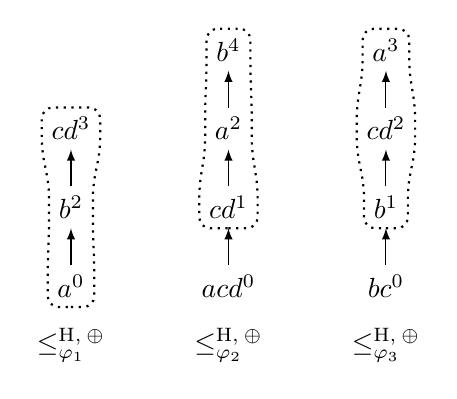
\begin{tikzpicture}
			\node at (0,-0.75){$\le^{\hamming,\:\agg}_{\phi_{1}}$};
			\node at (0,0)(a){$a^{0}$};
			\node at (0,1)(b){$b^{2}$};
			\node at (0,2)(cd){$cd^{3}$};
			\path[-latex](a)edge(b)(b)edge(cd);
			\draw[thick,dotted,rounded corners=4]
				(a.south)--
				(a.south east)--
				(a.north east)--
				(b.south east)--
				(b.north east)--
				(cd.south east)--
				(cd.north east)--
				(cd.north)--
				(cd.north west)--
				(cd.south west)--
				(b.north west)--
				(b.south west)--
				(a.north west)--
				(a.south west)--
				(a.south);

			\node at (2,-0.75){$\le^{\hamming,\:\agg}_{\phi_{2}}$};
			\node at (2,0)(acd){$acd^{0}$};
			\node at (2,1)(cd){$cd^{1}$};
			\node at (2,2)(a){$a^{2}$};
			\node at (2,3)(b){$b^{4}$};
			\path[-latex](acd)edge(cd)(cd)edge(a)(a)edge(b);
			\draw[thick,dotted,rounded corners=4]
				(cd.south)--
				(cd.south east)--
				(cd.north east)--
				(a.south east)--
				(a.north east)--
				(b.south east)--
				(b.north east)--
				(b.north)--
				(b.north west)--
				(b.south west)--
				(a.north west)--
				(a.south west)--
				(cd.north west)--
				(cd.south west)--
				(cd.south);

			\node at (4,-0.75){$\le^{\hamming,\:\agg}_{\phi_{3}}$};
			\node at (4,0)(bc){$bc^{0}$};
			\node at (4,1)(b){$b^{1}$};
			\node at (4,2)(cd){$cd^{2}$};
			\node at (4,3)(a){$a^{3}$};
			\path[-latex](bc)edge(b)(b)edge(cd)(cd)edge(a);
			\draw[thick,dotted,rounded corners=4]
				(b.south)--
				(b.south east)--
				(b.north east)--
				(cd.south east)--
				(cd.north east)--
				(a.south east)--
				(a.north east)--
				(a.north)--
				(a.north west)--
				(a.south west)--
				(cd.north west)--
				(cd.south west)--
				(b.north west)--
				(b.south west)--
				(b.south);
		\end{tikzpicture}			
	\end{minipage}
	\caption{
		Preorders generated using Hamming distances
		and an aggregation function $\agg$
		for the profile $\P=(\phi_i)_{1\le i \le 3}$.
		A majority cycle between $a$, $b$ and $cd$
		means that there is no weak Condorcet winner 
		with respect to $\P$ and $\mu$,
		for $[\mu]=\{a,b,cd\}$.
		The fact that none of the models of $\mu$ is 
		in the top choices of more than two agents in 
		$\P$ means that there is no majority-supported 
		outcome	with respect to $\P$ and $\mu$ outcome either.
	}
	\label{fig:5-condorcet-majr-empty}
\end{figure}

\begin{xmpl}{Weak Condorcet winners do not always exist}{5-condorcet-majr-empty}
	For the set of atoms $\Atoms=\{a,b,c,d\}$,
	consider a profile $\P=(\phi_i)_{1\le i \le 3}$,
	with $[\phi_{1}]=\{a\}$, $[\phi_{2}]=\{acd\}$ and $[\phi_{3}]=\{bc\}$,
	and a constraint $\mu$,
	with $[\mu]=\{a,b,cd\}$.
	The Hamming distances from each of the formulas in $\P$ to 
	each of the models of $\mu$, 
	together with the preorders $\le^{\hamming,\:\agg}_{\phi_{i}}$
	on the models of $\mu$,	for $i\in\{1,2,3\}$,
	are depicted in Figure \ref{fig:5-condorcet-majr-empty}.

	Note that there is no weak Condorcet winner with respect to $\P$ and $\mu$. 
	For instance, the support of $a$ over $b$ is $\supp^{\hamming,\:\agg}_{\mu}(a,b)=\{1,2\}$,
	while the support of $b$ over $a$ is $\supp^{\hamming,\:\agg}_{\mu}(b,a)=\{3\}$,
	which means that $a$ beats $b$ in a head to head election.
	However, $\supp^{\hamming,\:\agg}_{\mu}(a,cd)=\{1\}$ and $\supp^{\hamming,\:\agg}_{\mu}(cd,a)=\{2,3\}$,
	which means that $a$ loses to $cd$ in a head to head contest.
	The same holds for all other pairs of models of $\mu$.
	Likewise, there is no majority-supported outcome
	with respect to $\P$ and $\mu$,
	since none of the models of $\mu$ is in the top choices of more 
	than two of the agents in $\P$.
\end{xmpl}

Example \ref{ex:5-condorcet-majr-empty} shows that 
the postulates just introduced are best understood
by looking at what they expect of the preorders describing the profile.
To make this connection more precise, we present a set of 
properties meant to apply to an $\L^n$-assignment $\as$ on interpretations
that represents an $\L^{n}$-merging operator.
To make sense of the following properties, 
recall from Section \ref{sec:2-choice-functions} that a weak Condorcet winner
with respect to a preference profile and a set of alternatives is an alternative that
gets at least as much support as every other alternative in the set.
The following properties are meant to apply for any 
set $N=\{1,\dots, n\}$ of agents, $\L$-profile $\P=(\phi_i)_{1\le i \le n}$,
interpretations $w_1$ and $w_2$
and sets of interpretations $\W$, $\W_1$, $\W_2$:

\begin{description}
	\item[($\oom{\NOND}$)] There is no agent $i$ such that $\le_{\P}=\le_{\phi_i}$,
		for any profile $\P=(\phi_i)_{1\le i \le n}$.	
	\item[($\oom{\WPRT}$)] If $w_{1}\le_{\phi_i}w_2$, for all $i\in N$, then $w_1 \le_{\P} w_2$.
	\item[($\oom{\SPRT}$)] If $w_{1}\le_{\phi_i}w_2$, for all $i\in N$, 
	and there exists $j\in N$ such that $w_1<_{\phi_j}w_2$, then $w_1 <_{\P} w_2$.
	\item[($\oom{\CSOV}$)] There exists a profile $\P$ such that $w_1\le_{\P}w_2$,
	for any $w_1\in\W_1$ and $w_2\in\W_2$.
	\item[($\oom{\COND}$)] If $w$ is a weak Condorcet winner with respect to $(\le_{\phi_i})_{1\le i\le n}$ and $\W$, 
		then $w\le_\P w'$, for any $w'\in\W$.
	\item[($\oom{\MAJR}$)] If $w_1\le_{\phi_i}w_2$ for a majority of $i\in N$,
		then $w_1\le_{\P}w_2$.
\end{description}

An $\L$-assignment $\as$ on interpretations 
is \emph{non-dictatorial}, \emph{weak} and \emph{strong} Pareto efficient, 
\emph{Condorcet consistent} and \emph{majority consistent} if it satisfies 
properties $\oom{\NOND}$, $\oom{\WPRT}$, $\oom{\SPRT}$, $\oom{\COND}$ and $\oom{\MAJR}$,
respectively.
The properties just introduced map neatly onto the postulates presented earlier.
Since these postulates were tailored specifically to capture solution concepts
from voting theory, this comes as no surprise.

\begin{thm}{}{5-repr-evenhandedness}
	If $\me$ is an $\L^{n}$-merging operator that satisfies postulates $\ppm{0-1}$ and $\ppm{3}$
	and $\as$ is a total $\L^n$-assignment on interpretations that represents it,
	then the following equivalences hold:
	\begin{description}
		\item[(1)] $\me$ satisfies postulate $\ppm{\NOND}$ if and only if $\as$ satisfies property $\oom{\NOND}$.
		\item[(2)] $\me$ satisfies postulate $\ppm{\WPRT}$ if and only if $\as$ satisfies property $\oom{\WPRT}$.
		\item[(3)] $\me$ satisfies postulate $\ppm{\SPRT}$ if and only if $\as$ satisfies property $\oom{\SPRT}$.
		\item[(4)] $\me$ satisfies postulate $\ppm{\CSOV}$ if and only if $\as$ satisfies property $\oom{\CSOV}$.
		\item[(5)] $\me$ satisfies postulate $\ppm{\COND}$ if and only if $\as$ satisfies property $\oom{\COND}$.
		\item[(6)] $\me$ satisfies postulate $\ppm{\MAJR}$ if and only if $\as$ satisfies property $\oom{\MAJR}$.
	\end{description}
\end{thm}
\begin{prf*}{}{}%
	For a comment on the role of postulates $\ppm{0-1}$ and $\ppm{3}$, 
	see the comment at the beginning of the proof for Theorem \ref{thm:5-repr-insensitivity-syntax}.

	For Equivalence (1), we have that the existence of an agent $i$ 
	such that $\me_{\mu}(\P)=\me_{\mu}(\phi_{i})$,
	for any profile $\P=(\phi_i)_{1\le i \le n}$ and constraint $\mu$,
	is equivalent to the fact that 
	$w_1 \le_{\P}w_2$ if and only if $w_1 \le_{\phi_{i}}w_2$, for any interpretations $w_1$ and $w_2$,
	i.e., to the fact that $\le_{\P} = \le_{\phi_{i}}$.

	For Equivalence (2), suppose first that $\me$ satisfies postulate $\ppm{\WPRT}$ 
	and assume that $\as$ does not satisfy property $\oom{\WPRT}$.
	This means that there exist interpretations $w_1$ and $w_2$
	such that $w_1 \le_{\phi_{i}}$, for $i\in N$, and $w_2 \le_{\P}w_1$. 
	Taking the constraint $\px_{1,2}$ yields a contradiction with postulate $\ppm{\WPRT}$.
	Conversely, suppose $\as$ satisfies property $\oom{\WPRT}$ and $\me$ does not satisfy
	postulate $\ppm{\WPRT}$. This implies that there exists 
	$w_1\in[\me_{\mu}(\phi_{1})\land\dots\land \me_{\mu}(\phi_{n})]$
	such that $w_1\notin[\me_{\mu}(\P)]$.
	The latter conclusion implies,
	by postulates $\ppm{0}$ and $\ppm{1}$ and the assumption that 
	$\le_{\P}$ is total,
	that there exists an interpretation $w_2\in[\me_{\mu}(\P)]$
	such that $w_2 <_{\P}w_1$. 
	The former conclusion, however, implies that $w_1 \le_{\phi_{i}} w_2$, 
	for any $i\in N$,
	which, together with property $\oom{\WPRT}$, implies that $w_1 \le_{\P} w_2$.
	We have thus arrived at a contradiction.

	For Equivalence (3), suppose first that $\me$ satisfies postulate $\ppm{\SPRT}$ 
	and assume that $\as$ does not satisfy property $\oom{\SPRT}$.
	This means that there exist interpretations $w_1$ and $w_2$
	such that $w_1 \le_{\phi_{i}} w_2$, for $i\in N$, $w_1 <_{j}w_2$,
	for some $j\in N$ and, furthermore, that $w_2 \le_{\P} w_1$.
	This means that 
	$\me_{\px_{1,2}}(\phi_{1})\land\dots\land \me_{\px_{1,2}}(\phi_{n})$
	is consistent, which, by postulate $\ppm{\SPRT}$, implies that 
	$w_2\in[\me_{\px_{1,2}}(\phi_{j})]$.
	But this is a contradiction. 
	Conversely, suppose $\as$ satisfies property $\oom{\SPRT}$ and $\me$ does not satisfy
	postulate $\ppm{\SPRT}$. This implies that there exists an interpretation 
	$w_1\in[\me_{\mu}(\P)]$ such that $w_1\notin[\me_{\mu}(\phi_{1})\land\dots\land \me_{\mu}(\phi_{n})]$.
	The latter conclusion,
	together with postulates $\ppm{0}$, $\ppm{1}$ and the assumption that $\as$ is total,
	implies that there exists $j\in N$ such that 
	$w_1\notin[\me_{\mu}(\phi_{j})]$.
	The assumption that $\me_{\mu}(\phi_{1})\land\dots\land \me_{\mu}(\phi_{n})$
	is consistent implies that there exists $w_2\in[\me_{\mu}(\phi_{1})\land\dots\land \me_{\mu}(\phi_{n})]$.
	Putting the last two facts together implies that 
	$w_2\le_{\phi_i}w_1$, for every $i\in N$, and $w_2<_{\phi_{j}}w_1$,
	which, by property $\oom{\SPRT}$, yields that $w_2<_{\P}w_1$.
	But this contradicts the fact that $w_1\in[\me_{\mu}(\P)]$.

	For Equivalence (4), the statement is trivially true if $\mu_1\land\mu_2$ is inconsistent,
	hence we only look at the case when $\mu_1\land\mu_2$ is consistent.
	For one direction, suppose $\me$ satisfies postulate $\ppm{\CSOV}$:
	then, for any sets $\W_1$ and $\W_2$ of interpretations, take 
	the $\L$-proxies of $\W_1\cup\W_2$ and $\W_1$,
	i.e., two propositional formulas $\px_{\W_1\cup\W_2}$ and $\px_{\W_1}$ such that 
	$[\px_{\W_1\cup\W_2}]=\W_1\cup\W_2$ and $[\px_{\W_1}]=\W_1$.
	Using postulate $\ppm{\CSOV}$, we have that there exists a profile $\P$ 
	such that $\me_{\px_{\W_1\cup\W_2}}(\P)\land\px_{\W_1}\equiv \px_{\W_1\cup\W_2}\land\px_{\W_1}$,
	which implies that $[\me_{\px_{\W_1\cup\W_2}}(\P)]=\W_1$.
	This, in turn, implies that $\min_{\le_{\P}}[\px_{\W_1\cup\W_2}]=\W_1$,
	from which the conclusion follows.
	Conversely, we take $\W_1=[\mu_1\land\mu_2]$ and $\W_2=[\mu_1]$.

	For Equivalence (5), we remark that $w_1 \le^{\me}_{\P}w_2$
	is equivalent to $w_1\in[\me_{\px_{1,2}}(\P)]$, 
	which is equivalent to the fact that $w_1\in\min_{\le_{\P}}[\px_{1,2}]$,
	or $w_1{\le_{\P}}w_2$,
	for any total preorder $\le_{\P}$ used to represent $\me$.
	This implies that an interpretation $w^{\ast}$ being a weak Condorcet winner
	with respect to $(\le_{\phi_i})_{1\le i \le n}$ and $\mu$ is equivalent 
	to $w^{\ast}$ being a weak Condorcet winner with respect to the preference
	profile $\PP=(\le_{\phi_{i}})_{1\le i \le n}$ and $[\mu]$.
	If $\me$ is an $\L^{n}$-merging operator that satisfies postulate $\ppm{\COND}$,
	then a weak Condorcet winner $w^{\ast}$ with respect to $\PP$ and a set of interpretations 
	$\W$ will be a model of $\me_{\px_{\W}}(\P)$, and this implies that 
	$w^{\ast}\in\min_{\le_{\P}}[\px_{\W}]$,
	i.e., that $w^{\ast} \le_{\P} w$, for any interpretation $w\in[\W]$.
	Conversely, a weak Condorcet winner $w^{\ast}$ with respect to $\P$ and $\mu$
	is a weak Condorcet winner with respect to 
	$(\le_{\phi_i})_{1\le i \le n}$ and $[\mu]$ and, by property $\oom{\COND}$, it holds that 
	$w^{\ast}\le_{\P}w$, for any $w\in[\mu]$,
	which implies that $w^{\ast}\in\min_{\le_{\P}}[\mu]$,
	or $w^{\ast}\in[\me_{\mu}(\P)]$.

	For Equivalence (6) we use the same observation as above to argue that 
	$w^{\ast}$ being a majority-supported outcome with respect to $\P$ and $\mu$
	is equivalent to $w^{\ast}$ being a majority-supported outcome with respect 
	to $(\le_{\phi_i})_{1\le i \le n}$ and $[\mu]$, which then yields the conclusion.
\end{prf*}

Theorem \ref{thm:5-repr-evenhandedness} makes it clear what an $\L$-assignment $\as$ on interpretations
needs to look like if a merging operator $\me$ represented by it 
is to satisfy the postulates introduced in this section.
The immediate next question, however, is whether existing distance-based 
merging operators actually manage to select majority-supported outcomes, when they exist,
or weak Condorcet winner, when they exist, or whether they are non-dictatorial or resolvable.
For some of these properties there exists a useful shortcut,
since it turns out that they follow directly from postulate $\ppm{0-8}$.

\begin{prp}{}{5-nond-csov-prt}
	If $\me$ is an $\L^{n}$-merging operator that satisfies postulates $\ppm{0-8}$,
	then $\me$ also satisfies postulates $\ppm{\NOND}$, $\ppm{\CSOV}$, $\ppm{\WPRT}$ and $\ppm{\SPRT}$.
\end{prp}
\begin{prf*}{}{}%
	For postulate $\ppm{\NOND}$,
	suppose agent 1, with beliefs $\phi_1$, is a dictator for the merging operator $\me$. 
	Choose a formula $\phi_2$ such that $\phi_1 \land \phi_2$ is inconsistent 
	and a constraint $\mu = \phi_1 \lor \phi_2$.
	Since agent 1 is a dictator, we have that $\me_{\mu}(\phi_1, \phi_2)\equiv \me_{\mu}(\phi_1)$.
	Since $\mu \land \phi_1 $ is consistent, by postulate $\ppm{2}$ 
	it follows that $\me_{\mu}(\phi_1) \equiv \phi_1\land \mu \equiv \phi_1$. 
	At the same time we have that $\me_\mu(\phi_1,\phi_2) \land \phi_1$ is consistent, 
	and thus, by postulate $\ppm{4}$, 
	it holds that $\me_{\mu}(\phi_1,\phi_2) \land \phi_2$ is consistent as well. 
	We then have a contradiction with the fact that $\phi_1 \land \phi_2$ is inconsistent.

	For postulate $\ppm{\CSOV}$,
	if $\mu_1\land\mu_2$ is inconsistent, the conclusion is immediate.
	If $\mu_1\land\mu_2$ is consistent,
	take a profile $\P = (\phi)$,
	where $\phi=\mu_1\land\mu_2$.
	Clearly, $\phi \land \mu_1$ is consistent, hence by postulate $\ppm{2}$ 
	it follows that $\me_{\mu}(\P) \equiv \phi\land\mu_1\equiv\mu_1\land\mu_2$.

	Postulates $\ppm{\WPRT}$ and $\ppm{\SPRT}$ follow directly from postulates $\ppm{5}$ and $\ppm{6}$.
\end{prf*}

In the case of postulate $\ppm{\MAJR}$, the situation turns out to be different:
the presence of postulate $\ppm{2}$ actually precludes any merging operator 
from satisfying $\ppm{\MAJR}$.

\begin{prp}{}{5-majr}
	If $\me$ is an $\L^{n}$-merging operator that satisfies postulate $\ppm{2}$, 
	then $\me$ does not satisfy postulate $\ppm{\MAJR}$.
\end{prp}
\begin{prf*}{}{}%
	Take a profile $\P=(\phi_i)_{1\le i \le 3}$,
	with $[\phi_{1}]=[\phi_2]=\{\emptyset,a\}$
	and $[\phi_{3}]=\{\emptyset\}$, 
	and a constraint $\mu$ with $[\mu]=\{\emptyset,a\}$.
	Postulate $\ppm{2}$ implies that 
	$[\me_{\mu}(\P)]=[\phi_1\land\phi_2\land\phi_3\land\mu]=\{\emptyset\}$.
	Thus, even though $a$ is a top choice of two out of the three agents,
	$a$ does not make the list of winning interpretations.
\end{prf*}

The idea behind Proposition \ref{prop:5-majr} is that, under postulate $\ppm{2}$,
any agent has veto power over an interpretation $w$: by not including $w$ 
in its top choices, i.e., by not making $w$ a model of its submitted opinion, 
the agent makes sure that $w$ is not part of the result:
and this will happen even if $w$ is supported by a majority of the agents. 
Incidentally, postulate $\ppm{2}$ precludes the possibility that anything along the lines
of a \emph{plurality-supported outcome} will be guaranteed to be in the result. 

We now have all the pieces of information we need to 
determine where the main distance-based operators 
stand in relation to the postulates introduced in this section.

\begin{table}\centering
	\begin{tabular}{ccccccc}
		\toprule
						 & $[\phi_{1-3}]$ & $[\phi_{4-5}]$ & $[\phi_{6}]$ & $[\phi_{7}]$ &&\\
		$\dd_{\hamming}$ & $3\cdot\{a\}$     & $2\cdot\{bc\}$ & $\{b\}$ & $\{acd\}$ & $\dd_{\hamming}^{\ssum}(\P,\bullet)$ & $\dd_{\hamming}^{\leximax}(\P,\bullet)$\\
																 \midrule
			$a$          &     $3\cdot 0$     &   $2\cdot 3$        & $2$ & $2$ & $10$ & $(3,3,2,2,0,0,0)$   \\
			$b$          &     $3\cdot 1$     &   $2\cdot 1$        & $0$ & $4$ & $\mathbf{9}$  & $(4,1,1,1,1,1,0)$   \\
			$cd$          &    $3\cdot 2$     &   $2\cdot 2$        & $3$ & $1$ & $14$ & $\mathbf{(3,2,2,2,2,2,1)}$   \\
			\bottomrule
	\end{tabular}	
	\caption{
		Outcome $a$ is the only weak Condorcet winner 
		with respect to	the profile $\P=(\phi_i)_{1\le i \le 7}$ 
		and $\mu$, where $[\mu]=\{a,b,cd\}$,
		but $a$ is selected by neither $\me^{\hamming,\:\ssum}$
		nor by $\me^{\hamming,\:\leximax}$.
	}
	\label{tab:5-hsum-hlmax-not-condorcet}
\end{table}

\begin{prp}{}{5-dist-ops-evenhandedness}
	If $\agg$ is either the $\ssum$, $\leximax$ or $\leximin$
	aggregation function, then the following statements hold:
	\begin{description}
		\item[(1)] postulates $\ppm{\NOND}$, $\ppm{\WPRT}$, $\ppr{\SPRT}$ and $\ppm{\CSOV}$
		are satisfied by all operators $\me^{\hamming,\:\agg}$ and $\me^{\drastic,\:\agg}$;
		\item[(2)] postulate $\ppm{\COND}$ is satisfied by operators $\me^{\drastic,\:\agg}$,
			but by neither of the operators $\me^{\hamming,\:\agg}$;
		\item[(3)] postulate $\ppm{\MAJR}$ is satisfied by neither of the operators $\me^{\drastic,\:\agg}$
			and $\me^{\hamming,\:\agg}$.
	\end{description}
\end{prp}
\begin{prf*}{}{}%
	Since the operators $\me^{\hamming,\:\agg}$ 
	and $\me^{\drastic,\:\agg}$, 
	for $\agg\in\{\ssum,\leximax,\leximin\}$, 
	satisfy postulates $\ppm{0-8}$, then,
	by Proposition \ref{prop:5-nond-csov-prt}, they 
	also satisfy postulates $\ppm{\NOND}$, $\ppm{\WPRT}$, $\ppr{\SPRT}$, $\ppm{\CSOV}$,
	and by Proposition \ref{prop:5-majr} they do not satisfy 
	postulate $\ppm{\MAJR}$.
	This shows that Statements (1) and (3) hold.

	For Statement (2) and operators $\me^{\drastic,\:\agg}$ recall first that 
	all three operators considered here are equivalent,
	so proving the claim for $\me^{\drastic,\:\ssum}$ will suffice. 
	Note, as well, that $\dd_{\drastic}^{\ssum}(\P,w)$ essentially 
	counts the number of agents in $N$,
	who have $w$ as their model, for any interpretation $w$,
	and $\me^{\drastic,\:\ssum}$ selects the interpretations in $[\mu]$
	that occur most often as models of agents in $N$.
	We have, then, that if $w^{\ast}$ is a weak Condorcet winner with respect 
	to $\phi$ and $\mu$, then $\supp^{\drastic,\:\ssum}_{\mu}(w^{\ast},w)\ge\supp^{\drastic,\:\ssum}(w,w^{\ast})$,
	for any interpretation $w\in[\mu]$.
	This means that $w^{\ast}$ occurs as a model of $\phi_{i}$ for at least as many 
	agents $i\in N$ than any other interpretation $w\in[\mu]$,
	which, as per the previous observation, implies that $w^{\ast}\in[\me^{\drastic,\:\ssum}_{\mu}(\P)]$.	 

	For Statement (2) and operators $\me^{\hamming,\:\ssum}$ and $\me^{\hamming,\:\leximax}$, 
	take the profile $\P=(\phi_i)_{1\le i \le 7}$,
	with $[\phi_{1}]=[\phi_{2}]=[\phi_{3}]=\{a\}$,
	$[\phi_{4}]=[\phi_{5}]=\{bc\}$,
	$[\phi_{6}]=\{b\}$,
	$[\phi_{7}]=\{acd\}$,
	and a constraint $\mu$ such that 
	$[\mu]=\{a,b,cd\}$.
	The Hamming distances from $\phi_{i}$, for $1\le i\le 7$,
	to every model of $\mu$,
	together with the aggregated distances for 
	the $\ssum$ and $\leximax$ aggregation function, 
	are depicted in Table \ref{tab:5-hsum-hlmax-not-condorcet}.

	Note that $a$ is the only weak Condorcet winner with respect to 
	$\P$ and $\mu$, since the size of its support over $b$ and $cd$
	is $4$ in both cases. 
	In other words, $[\COND_{\mu}(\P)]=\{a\}$.
	However, $a$ is selected by neither $\me^{\hamming,\:\ssum}$
	nor $\me^{\hamming,\:\leximax}$, since $[\me^{\hamming,\:\ssum}_{\mu}(\P)]=\{b\}$
	and $[\me^{\hamming,\:\leximax}_{\mu}(\P)]=\{cd\}$.

	For Statement (2) and operator $\me^{\hamming,\:\leximin}$,
	a simpler counterexample will suffice. 
	Take the profile $\P=(\phi_i)_{1\le i \le 3}$,
	with $[\phi_{1}]=[\phi_{2}]=\{\emptyset\}$ and $[\phi_{3}]=\{ab\}$,
	and a constraint $\mu$ with $[\mu]=\{a,ab\}$.
	We have that 
	$\dd_{\hamming}^{\leximin}(\P,a)=(1,1,1)$
	and
	$\dd_{\hamming}^{\leximin}(\P,ab)=(0,2,2)$,
	which means that $[\me^{\hamming,\:\leximin}_{\mu}(\P)]=\{ab\}$.
	However, $a$ is the only weak Condorcet winner 
	(and even the majority supported outcome)
	with respect to $\P$ and $\mu$.
\end{prf*}
























\section{Responsiveness}\label{sec:5-responsiveness}
This section proposes an assortment of properties 
meant to ensure that changes in the profile 
produce an intuitive, and expected, change of the outcome,
i.e., that the merging operation is responsive to 
the structure of the profile.
Since these properties involve expanding the set $N=\{1,\dots,n\}$ 
of agents in the profile
%  and the set $\Atoms$ of atoms, 
we need to make sure that there is a stock of agents 
% and atoms 
on hand if needed to supplement the profile 
% and $\Atoms$ 
with new elements.
We assume, therefore, that the set of agents $N$
who supply formulas to the merging operator 
% and $\Atoms$ are 
is part of some larger subsets,
whose elements can be invoked upon request.
% Adding atoms to $\Atoms$ is akin to the idea  adding a candidate to an election.
That being said, we can introduce the following postulates,
intended to hold for any profile
$\P=(\phi_i)_{1\le i \le n}$, 
and constraints $\mu$, $\mu_1$, $\mu_2$:
% and atoms $p$ and $q$:

\begin{description}
	\item[($\ppm{\MONO}$)] $\me_{\mu}(\P + \phi_{n+1}) \land \me_{\mu}(\phi'_{n+1})\models\me_{\mu}(\P+\phi'_{n+1})$.
 
	\item[($\ppm{\PART}$)] If $\me_\mu(\P) \land \phi_{n+1}$ is consistent, 
		then $\me_\mu(\P) \land \phi_{n+1} \models \me_{\mu}(\P+\phi_{n+1})$. 

	\item[($\ppm{\RSYM}$)] If $\me_\mu(\P)$ is complete and $\mu$ has more than one model, 
		then $\me_\mu(\phi_1,\dots,\phi_n) \nvDash\me_{\mu}(\lnot\phi_1,\dots,\lnot\phi_n)$.

	\item[($\ppm{\RSVB}$)] If $\me_{\mu_1}(\P)\land\mu_2$ is consistent, 
		there is $\phi_{n+1}$ such that $\me_{\mu_1}(\P+\phi_{n+1})\equiv \me_{\mu_1}(\P)\land \mu_2$.

	% \item[($\ppm{\INDC}$)] If $p\in\Atoms$ and $q\notin\Atoms$, 
	% 	then $\me_\mu(\phi_1,\dots,\phi_n) \equiv \me_{\mu}(\phi_1\land(p\leftrightarrow q),\dots,\phi_n\land(p\leftrightarrow q))$. 

	% \item[($\ppm{\CONS}$)] $\me_{\mu}(\P_1) \land \dots \land \me_{\mu}(\P_n) \models \me_\mu(\P_1+\dots+\P_n)$.

	% \item[($\ppm{\HOMG}$)] $\me_\mu(\P) \equiv \me_{\mu}(\P+\dots+\P)$.

	% \item[($\ppm{\SLFA}$)] $\me_{\mu}(\P +\me_\mu(\P)) \equiv \me_\mu(\P)$.
\end{description}

Postulate $\ppm{\MONO}$, where `$\MONO$' stands for \emph{monotonicity},
says that if $\phi_{n+1}$ agrees with the profile $\P+\phi_{n+1}$ 
to a certain extent when the constraint is $\mu$,
then this agreement is carried over when merging the formulas in the profile $\P+\phi'_{n+1}$.
Intuitively, the profile $\P+\phi'_{n+1}$ can be thought of as being obtained from 
the profile $\P+\phi_{n+1}$ by replacing $\phi_{n+1}$ with $\phi'_{n+1}$:
it is as if agent $n+1$ considers its options, 
changes its mind and submits $\phi'_{n+1}$ instead of $\phi_{n+1}$.
Postulate $\ppm{\MONO}$ then says that if this change of mind
(i.e., after submitting $\phi'_{n+1}$)
is in line with the 
result obtained previously
(i.e., when submitting $\phi_{n+1}$), then the originally agreed upon result 
should not be changed. 
In other words, if the agent maintains its support 
for a raft of issues that were already included 
in the final result, then these issues are still endorsed
by the merging process
when the agent submits a formula that expresses as much, if not more, 
support for these issues.
In this, postulate $\ppm{\MONO}$ attempts to recreate the monotonicity property 
found in voting theory:
a voting system is monotone if the winning alternative in an election cannot be 
turned into a non-winner by one voter moving this alternative up in its ranking, 
while keeping the rest of the ranking fixed.
The intuition behind our formalization stems from seeing the models of 
$\me_\mu(\P)$ as the winners in the election where the models of $\mu$ 
are candidates and the formulas in $\P$ are the voters,
and will come out more clearly when modeled 
as a property for assignments on interpretations,
to come shortly.
% Thus, if any candidates elected by the profile $\P_1+ \P_2$ are also elected by the profile $\P_3$ alone, 
% then monotonicity would require that the same  candidates should also be elected when we replace $\P_2$ with $\P_3$ in $\P_1 + \P_2$.
% The idea, to put it succinctly, is that a winner stays a winner, if its position is only increased in the votes. 
Note that postulate $\ppm{\MONO}$ as put forward here is slightly 
different from the way it was originally presented \cite{HaretPW16}.
The change is made in order to bring the postulate closer to the monotonicity
property as featured in social choice. Though arguable whether the present formulation
achieves this completely, it is certainly an interesting property to consider.

Postulate $\ppm{\PART}$, where `$\PART$' stands for \emph{participation},
refers to a phenomenon that in voting is linked to the \textit{no-show paradox}.
A voting rule is vulnerable to this type of paradox
if it is possible to change the winner from candidate $c_i$ to candidate $c_j$ 
by adding a vote in which candidate $c_i$ is strictly preferred to candidate $c_j$.
In a merging scenario, we prevent this by adding a formula $\phi$ to a given profile $\P$ and
requiring that $\me_{\mu}(\P+\phi)$ should not be `worse' than $\me_\mu(\P)$ with respect to $\phi$.

Postulate $\ppm{\RSYM}$, where `$\RSYM$' stands for \emph{reversal symmetry},
harkens back to an eponymous property in voting.
A voting rule satisfies reversal symmetry if the 
winner (assumed to be unique) of an election does not stay a winner
if all votes are reversed.
In a merging scenario, we interpret the condition of having a unique winner 
as the outcome of merging 
being a complete formula (i.e., a formula with exactly one model), 
and we take reversing the vote to mean that every formula 
is replaced with its negation.
% Notice that we require the outcome to be a complete formula to reflect the requirement 
% of a unique winner in the voting setting.

Postulate $\ppm{\RSVB}$, where `$\RSVB$' stands for \emph{resolvability},
says that the output of merging can be refined up to an arbitrary degree 
by adding just one formula to $\P$.
In a voting scenario resolvability 
requires that any winner can be made 
the unique winner by adding a single vote \cite{Tideman06},
and postulate $\ppm{\RSVB}$ models this intuition. 


% Postulate $\ppm{\INDC}$ concerns \emph{independence of clones}.
% In voting theory two candidates are clones if they are ranked next to each other, and in the same pattern, in all votes.
% A voting system is independent of clones if a non-winning candidate cannot be made a winner by adding clones to the election. 
% In a merging scenario we think of a clone as a fresh variable $q$ that mirrors an existing variable $p$,
% in the sense that agents uniformly consider them as equivalent, i.e., can adopt $p\leftrightarrow q$ as part of the belief. 
% Postulate $\ppm{\INDC}$ requires that the merging result does not change when adding a clone to a profile. 

% Postulate $\ppm{\CONS}$ concerns \emph{consistency},
% which in a voting scenario requires that if an election is arbitrarily divided into sub-elections 
% and there is a candidate $c$ that is a winner in all of the them, then $c$ is also a winner in the original election.
% In a merging scenario, we formalize this by splitting the merging task across different profiles 
% ($\P_1$, \dots, $\P_n$), which can be thought of as parts of a larger profile ($\P_1+\dots+\P_n$). 
% Postulate $\ppm{\CONS}$ then requires that any outcomes universally accepted across the subprofiles
% are also accepted in the profile obtained by concatenating them.

% Postulate $\ppm{\HOMG}$ concerns \emph{homogeneity},
% which in a voting system requires that the result cannot be changed by duplicating each vote a number of times. 
% In a merging scenario this translates as postulate $\ppm{\HOMG}$, 
% saying that the outcome of merging does not change if the profile is expanded by multiple copies of itself. 

% Postulate $\ppm{\SLFA}$ concerns \emph{self agreement},
% and requires that the merging outcome stays the same if $\P$ is added back to the profile and the merging 
% process is run again.

With the postulates in place, we want to switch now to the semantic
view, and see how the postulates are represented at the level off
an $\L$-assignment $\as$ on interpretations.
Thus, given such an assignment, 
consider the following properties,
expected to hold for any $\L$-profile $\P=(\phi_i)_{1\le i \le n}$,
propositional formulas $\phi_{n+1}$, $\phi'_{n+1}$,
sets $\W_1$ and $\W_2$ of interpretations
and interpretations $w_1$ and $w_2$:

\begin{description}
	\item[($\oom{\MONO}$)] If $w_1\le_{\P_1+\phi_{n+1}}w_2$ and $w_1\le_{\phi'_{n+1}}w_2$, then $w_1\le_{\P+\phi'_{n+1}}w_2$.
	\item[($\oom{\PART}$)] If $w_1 \le_{\P}w_2$ and $w_1\in[\phi_{n+1}]$, then $w_1 \le_{\P+\phi_{n+1}}w_2$. 
	\item[($\oom{\RSYM}$)] If $w_1 <_{(\phi_i)_{1\le i \le n}}w_2$, then $w_2<_{(\lnot\phi_i)_{1\le i \le n}}w_1$. 
	\item[($\oom{\RSVB}$)] If $w_1 \le_{\P}w_2$, for every interpretation $w_1\in\W_1$ and $w_2\in\W_2$,
		then there exists a formula $\phi_{n+1}$ such that $w_1<_{\P+\phi_{n+1}}w_2$, 
		for every interpretation $w_1\in\W_1$ and $w_2\in\W_2$.
\end{description}

\begin{thm}{}{5-repr-responsiveness}
	If $\me$ is an $\L^{n}$-merging operator satisfying postulates $\ppm{0-1}$ and $\ppm{3}$,
	and $\as$ is a total $\L^n$-assignment on interpretations that represents it,
	then the following equivalences hold:
	\begin{description}
		\item[(1)] $\me$ satisfies postulate $\ppm{\MONO}$ if and only if $\as$ satisfies property $\oom{\MONO}$.
		\item[(2)] $\me$ satisfies postulate $\ppm{\PART}$ if and only if $\as$ satisfies property $\oom{\PART}$.
		\item[(3)] $\me$ satisfies postulate $\ppm{\RSYM}$ if and only if $\as$ satisfies property $\oom{\RSYM}$.
		\item[(4)] $\me$ satisfies postulate $\ppm{\RSVB}$ if and only if $\as$ satisfies property $\oom{\RSVB}$.
	\end{description}
\end{thm}
\begin{prf*}{}{}%
	For Equivalence (1), suppose first that $\me$ satisfies postulate $\ppm{\MONO}$
	and take interpretations $w_1$ and $w_2$ such that 
	$w_1 \le_{\P+\phi_{n+1}}w_2$ and $w_1 \le_{\phi'_{n+1}}w_2$.
	This implies that $w_1\in\min_{\le_{\P+\phi_{n+1}}}[\px_{1,2}]$ and $w_1\in\min_{\le_{\phi'_{n+1}}}[\px_{1,2}]$,
	i.e., that $w_1\in[\me_{\px_{1,2}}(\P+\phi_{n+1})\land \me_{\px_{1,2}}(\phi'_{n+1})]$.
	Using postulate $\ppm{\MONO}$, we conclude that $w_1\in[\me_{\px_{1,2}}(\P+\phi'_{n+1})]$.
	From this it follows that $w_1\le_{\P+\phi'_{n+1}}w_2$.
	Conversely, suppose $\as$ satisfies property $\oom{\MONO}$ and 
	$\me_{\mu}(\P+\phi_{n+1})\land \me_{\mu}(\phi'_{n+1})$ is consistent.
	The latter fact implies that there exists an interpretation 
	$w_1\in[\me_{\mu}(\P+\phi_{n+1})\land \me_{\mu}(\phi'_{n+1})]$.
	Taking an arbitrary interpretation $w_2\in[\mu]$ and applying property $\oom{\MONO}$, 
	we conclude that 
	$w_1 \le_{\P+\phi'_{n+1}}w_2$, which implies that $w_1\in[\me_{\mu}(\P+\phi'_{n+1})]$.

	For Equivalence (2), suppose $\me$ satisfies postulate $\ppm{\PART}$
	and take two interpretations $w_1$ and $w_2$ such that $w_1 \le_{\P} w_2$.
	We then obtain that $w_1\in[\me_{\px_{1,2}}(\P)\land\phi_{n+1}]$, 
	which, by postulate $\ppm{\PART}$, implies that $w_1\in[\me_{\px_{1,2}}(\P+\phi_{n+1})]$
	and hence $w_1 \le_{\P+\phi_{n+1}}w_2$.
	Conversely, if $\as$ satisfies property $\oom{\PART}$, 
	then for any $w_1\in[\me_{\mu}(\P)\land\phi_{n+1}]$ and 
	interpretation $w_2\in[\mu]$, it follows that $w_1 \le_{\P+\phi_{n+1}}w_2$,
	which implies the conclusion.

	For Equivalence (3), suppose $\me$ satisfies postulate $\ppm{\RSYM}$
	and take two distinct interpretations $w_1$ and $w_2$ such that $w_1 <_{(\phi_i)_{1\le i \le n}} w_2$.
	This implies that $[\me_{\px_{1,2}}(\phi_1,\dots,\phi_n)]=\{w_1\}$, i.e., that $\me_{\px_{1,2}}(\phi_1,\dots,\phi_n)$
	is complete. Applying postulate $\ppm{\RSYM}$, it follows that $[\me_{\px_{1,2}}(\lnot\phi_1,\dots,\lnot\phi_n)]=\{w_2\}$,
	showing that property $\oom{\RSYM}$ is satisfied.
	Conversely, if $\as$ satisfies property $\oom{\RSYM}$ and $[\me_{\mu}(\phi_1,\dots,\phi_n)]=\{w_1\}$,
	then $w_1<_{(\phi_i)_{1\le i \le n}}w_2$, for any other interpretation $w_2\in[\mu]$, which must exist as
	per the assumption of postulate $\ppm{\RSYM}$. Applying property $\oom{\RSYM}$ results in 
	$w_2<_{(\lnot\phi_i)_{1\le i \le n}}w_1$, which delivers the conclusion.	

	For Equivalence (4), suppose $\me$ satisfies postulate $\ppm{\RSVB}$
	and take sets of interpretations $\W_1$ and $\W_2$
	such that $w_1 \le_{\P}w_2$, for any $w_1\in\W_1$ and $w_2\in\W_2$.
	It follows that $\W_1\subseteq\min_{\le_{\P}}(\W_1\cup\W_2)$
	and hence that $[\me_{\px_{\W_1\cup\W_2}}(\P)\land \px_{\W_1}]=\W_1$.
	Postulate $\ppm{\RSVB}$ implies that there exists a formula 
	$\phi_{n+1}$ such that $\me_{\px_{\W_1\cup\W_2}}(\P+\phi_{n+1})\equiv\me_{\px_{\W_1,\W_2}}(\P)\land\px_{\W_1}$,
	from which it follows that $[\me_{\px_{\W_1\cup\W_2}}(\P+\phi_{n+1})]=\W_1$,
	and hence $w_1<_{\P+\phi_{n+1}}w_2$,
	for any $w_1\in\W_1$ and $w_2\in\W_2$.
	Conversely, suppose $\as$ satisfies property $\oom{\RSYM}$
	and take formulas $\mu_1$ and $\mu_2$ such that $\me_{\mu_1}(\P)\land\mu_2$
	is consistent.
	This implies that $w_1 \le_{\P}w_2$, for every $w_1\in\min_{\le_{\P}}[\mu_1]\cap[\mu_2]$
	and $w_2\in[\mu_1]$ and hence, by property $\oom{\RSVB}$,
	that there exists a formula $\phi_{n+1}$ such that 
	$w_1 <_{\P+\phi_{n+1}}w_2$, for every $w_1\in\min_{\le_{\P}}[\mu_1]\cap[\mu_2]$
	and $w_2\in[\mu_1]$.
	From this it follows that $\me_{\mu_1}(\P+\phi_{n+1})\equiv \me_{\mu_1}(\P)\land \mu_2$
\end{prf*}

\begin{prp}{}{5-part-rsvb}
	If $\me$ is an $\L^{n}$-merging operator that satisfies postulates $\ppm{0}$ and $\ppm{1}$,
	then the following statements hold:
	\begin{description}
		\item[($1$)] if $\me$ satisfies postulates $\ppm{2}$ and $\ppm{5}$, 
			then $\me$ satisfies postulate $\ppm{\PART}$.
		\item[($2$)] if $\me$ satisfies postulates $\ppm{2}$, $\ppm{5}$ and $\ppm{6}$ 
			then $\me$ satisfies postulate $\ppm{\RSVB}$.
	\end{description}
\end{prp}
\begin{prf*}{}{}%
	For Statement (1), take $w\in[\me_{\mu}(\P)\land\phi_{n+1}]$.
	By postulate $\ppm{0}$ it follows that $w\in[\mu]$.
	Since $w\in[\phi_{n+1}\land\mu]$, then by postulate $\ppm{2}$ 
	we can conclude that $w\in[\me_{\mu}(\phi_{n+1})]$
	and thus that $w\in[\me_{\mu}(\P)\land\me_{\mu}(\phi_{n+1})]$.
	Using postulate $\ppm{5}$ it follows that $w\in[\me_{\mu}(\P+\phi_{n+1})]$.

	For Statement (2), take $\phi_{n+1}\equiv \me_{\mu_1}(\P)\land\mu_2$.
	Both postulates $\ppm{0}$ and $\ppm{1}$ we have that 
	$(\me_{\mu_1}(\P)\land\mu_2)\land\mu_1\equiv\me_{\mu_1}(\P)\land\mu_2$,
	Thus, using postulate $\ppm{2}$, we have that 
	$\me_{\mu_1}(\me_{\mu_1}(\P)\land\mu_2)\equiv \me_{\mu_1}(\P)\land\mu_2$.
	This shows, among other things, that
	$\me_{\mu_1}(\P)\land \me_{\mu_1}(\me_{\mu_1}(\P)\land\mu_2)$ is consistent,
	which,
	by postulates $\ppm{5}$ and $\ppm{6}$ implies that
	$\me_{\mu_1}(\P)\land \me_{\mu_1}(\me_{\mu_1}(\P)\land\mu_2)\equiv \me_{\mu_1}(\P+(\me_{\mu_1}(\P)\land\mu_2))$.
	Using the previously derived equivalences,
	we can conclude that 
	$\me_{\mu_1}(\P)\land \me_{\mu_1}(\me_{\mu_1}(\P)\land\mu_2)\equiv \me_{\mu_1}(\P)\land\mu_2$.
\end{prf*}

Before laying down the full picture of how existing merging operators 
fare with respect to the postulates in this section,
a quick observation on the reversal symmetry postulate $\ppm{\RSYM}$
will help make things clearer. Reflection on postulate $\ppm{\RSYM}$,
and even more so on its semantic counterpart, property $\oom{\RSYM}$,
shows that the demands it places on an assignment are considerable:
in particular, property $\oom{\RSYM}$ requires that 
replacing all formulas in an $\L$-profile $\P$ with their negation 
should reverse all strict comparisons in the preorder 
corresponding to the negated profile.
When coupled with the observation that negating the formulas 
in an $\L$-profile may create a profile equivalent to the original one,
this leads to the conclusion that the only feasible 
preorder that can represent such a situation is one 
in which all interpretations are on the same level.

\begin{lem}{}{5-rsym}
	If $\me$ is an $\L^{n}$-merging operator that satisfies 
	postulates $\ppm{0-1}$, $\ppm{3}$ and $\ppm{\RSYM}$, then 
	$\me_{\top}(\phi,\lnot\phi)\equiv\top$,
	for any propositional formula $\phi$.
\end{lem}
\begin{prf*}{}{}%
	We know, by Theorem \ref{thm:3-merging-repr}, that $\me$
	is represented by a total, syntax insensitive and m-faithful 
	$\L^n$-assignment $\as$ on interpretations.
	By Theorem \ref{thm:5-repr-responsiveness},
	we can also conclude that $\as$ satisfies property $\oom{\RSYM}$.
	Suppose, now, that there exists a propositional formula $\phi$
	such that $\me_{\top}(\P)\not\equiv\top$,
	where $\P$ is the $\L$-profile $\P=(\phi,\lnot\phi)$.
	This implies that there exist interpretations $w_1$ and $w_2$
	such that $w_1<_{\P}w_2$.
	By property $\oom{\RSYM}$, we conclude that $w_2<_{\P'}w_1$,
	where $\P'$ is the $\L$-profile $\P'=(\lnot\phi,\lnot(\lnot\phi))$.
	It is easy to see, however, that $\P$ and $\P'$ are equivalent profiles
	and hence, by postulate $\ppm{3}$,
	that $\me_{\mu}(\P)\equiv \me_{\mu}(\P')$,
	for any propositional formula $\mu$.
	But this implies that $\le_{\P}=\le_{\P'}$,
	which contradicts the conclusions derived previously.
\end{prf*}

With all these results in hand, we can now have a full picture
of how the main merging operators stand up 
against the responsiveness properties 
put forward in this section.

\begin{table}\centering
	\begin{tabular}{cccccc}
		\toprule
		 & $\P=(\phi_1)$ & $(\phi_2)$ &&&\\
		 & $\{\emptyset,a\}$ & $\{abc\}$ & $\dd_{\hamming}^{\ssum}(\P+\phi_2,\bullet)$ & $\dd_{\hamming}^{\leximax}(\P+\phi_2,\bullet)$ & $\dd_{\hamming}^{\leximin}(\P+\phi_2,\bullet)$\\\midrule
		$\emptyset$ & $0$ & $3$ & $3$ & $(3,0)$ & $(0,3)$\\
		$abc$       & $2$ & $0$ & $\mathbf{2}$ & $\mathbf{(2,0)}$ & $\mathbf{(0,2)}$\\
		\bottomrule
	\end{tabular}
	\caption{
		Hamming distances from $\P=(\phi_1)$ and $\phi_2$ to each model of $\mu$,
		with $[\phi_{1}]=\{\emptyset,a\}$, $[\phi_2]=\{abc\}$ and $[\mu]=\{\emptyset,abc\}$,
		together with the aggregated distances using the $\ssum$, $\leximax$ and $\leximin$
		aggregation functions.
	}
	\label{tab:5-mono-1}
	vspace{1.5em}

	\begin{tabular}{cccccc}
		\toprule
		 & $\P=(\phi_1)$ & $(\phi'_2)$ &&&\\
		 & $\{\emptyset,a\}$ & $\{ab\}$ & $\dd_{\hamming}^{\ssum}(\P+\phi'_2,\bullet)$ & $\dd_{\hamming}^{\leximax}(\P+\phi'_2,\bullet)$ & $\dd_{\hamming}^{\leximin}(\P+\phi'_2,\bullet)$\\\midrule
		$\emptyset$ & $0$ & $2$ & $\mathbf{2}$ & $\mathbf{(2,0)}$ & $\mathbf{(0,2)}$\\
		$abc$       & $2$ & $1$ & $3$ & $(2,1)$ & $(1,2)$\\
		\bottomrule
	\end{tabular}
	\caption{
		Hamming distances from $\P=(\phi_1)$ and $\phi_2$ to each model of $\mu$,
		with $[\phi_{1}]=\{\emptyset,a\}$ as above, 
		$[\phi_2]=\{abc\}$ and $[\mu]=\{\emptyset,abc\}$,
		together with the aggregated distances using the $\ssum$, $\leximax$ and $\leximin$
		aggregation functions.
	}
	\label{tab:5-mono-2}
\end{table}

\begin{table}\centering
	\begin{tabular}{cccccc}
		\toprule
														 & 
		$\P$ 											 &  
		$\phi_{n+1}$ 									 & 
		$\phi'_{n+1}$ 									 & 
		$\dd_{\drastic}^{\ssum}(\P+\phi_{n+1},\bullet)$  & 
		$\dd_{\drastic}^{\ssum}(\P+\phi'_{n+1},\bullet)$ \\
				 										 \midrule
		$w_1$   & $k+1$ & $0$ & $0$ & $k+1$ & $k+1$\\
		$w_2$   & $k$   & $1$ & $0$ & $k+1$ & $k$\\
		\bottomrule
	\end{tabular}
	\caption{
		Drastic distances from $\P$, $\phi_{n+1}$ and $\phi'_{n+1}$ to $w_1$ and $w_2$,
		together with the aggregated distances using the $\ssum$ aggregation functions,
		for a stereotypical case that does not satisfy property $\oom{\MONO}$:
		outcome $w_1$ is winning after adding $\phi_{n+1}$ to $\P$,
		but it loses out to $w_2$ when agent $n+1$ submits a formula 
		that weakens the support for $w_1$.
	}
	\label{tab:5-mono-3}
\end{table}

\begin{prp}{}{5-dist-ops-responsiveness}
	If $\agg$ is either the $\ssum$, $\leximax$ or $\leximin$ aggregation function,
	then the following statements hold:
	\begin{description}
		\item [($1$)] merging operators $\me^{\hamming,\:\agg}$	and $\me^{\drastic,\:\agg}$
			all satisfy postulates $\ppm{\PART}$ and $\ppm{\RSVB}$;
		\item[($2$)] merging operators $\me^{\hamming,\:\agg}$ do not satisfy postulate $\ppm{\RSYM}$,
			but operators $\me^{\drastic,\:\agg}$ satisfy it;
		\item[($3$)] neither of the merging operators $\me^{\hamming,\:\agg}$ and $\me^{\drastic,\:\agg}$
			satisfies postulate $\ppm{\MONO}$;
		% \item[($4$)] neither of the merging operators $\me^{\hamming,\:\agg}$ and $\me^{\drastic,\:\agg}$
		% 	satisfies postulate $\ppm{\INDC}$.
	\end{description}
\end{prp}
\begin{prf*}{}{}%
	Statement (1) follows from Corollary \ref{cor:3-merging-d-agg-induced-operator},
	showing that all the operators considered here satisfy postulate $\ppm{0-8}$
	and Proposition \ref{prop:5-part-rsvb}, showing that these postulates guarantee 
	satisfaction of postulates $\ppm{\PART}$ and $\ppm{\RSVB}$.

	For Statement (2) and operators $\me^{\hamming,\:\agg}$,
	take the set of atoms $\Atoms=\{a,b\}$ and a profile $\P=(\phi_1,\phi_2)$,
	with $[\phi_{1}]=\{\emptyset,b,ab\}$ and $[\phi_{2}]=\{a\}$.
	Notice that $\me^{\hamming,\:\agg}_{\top}(\P)\not\equiv\top$,
	for all of the aggregation functions considered and thus,
	by Lemma \ref{lem:5-rsym}, the merging operators do not 
	satisfy postulate $\ppm{\RSYM}$.

	For Statement (2) and operators $\me^{\drastic,\:\agg}$,
	recall that operators $\me^{\drastic,\:\agg}$ are equivalent,
	for all aggregation functions considered here,
	and that the aggregated distance $\dd^{\agg}(\P,w)$ from an $\L$-profile $\P$
	to an interpretation $w$ essentially keeps track of the number of 
	formulas in $\P$ that have $w$ as their model;
	obviously, if we replace the formulas in $\P$ with their negation, then this number 
	is reversed. More precisely, if $\P'$ is the profile obtained by 
	replacing every formula in $\P$ with its negation, then 
	$\dd_{\drastic}^{\agg}(\P',w)=n-\dd_{\drastic}^{\agg}(\P,w)$, 
	where $n$ is the number of agents 
	in the profile. This implies that if $w_1<^{\drastic,\:\agg}_{\P}w_2$,
	then $w_2<^{\drastic,\:\agg}_{\P'}w_1$,
	for any interpretations $w_1$ and $w_2$,
	which shows that $\as^{\drastic,\:\agg}$ satisfies property $\oom{\RSYM}$
	and, by Theorem \ref{thm:5-repr-responsiveness},
	postulate $\ppm{\RSYM}$ as well.

	For Statement (3) and the operators $\me^{\hamming,\:\agg}$, 
	take the alphabet $\Atoms=\{a,b,c\}$,
	the $\L$-profile $\P=(\phi_1)$,
	with $[\phi_{1}]=\{\emptyset,a\}$, 
	the propositional formulas $\phi_{2}$ and $\phi'_{2}$
	with $[\phi_2]=\{abc\}$ and $[\phi'_2]=\{ab\}$,
	and a constraint $\mu$ with $[\mu]=\{\emptyset,abc\}$.
	The Hamming distances from $\P+\phi_2$ and $\P+\phi'_2$
	to each model of $\mu$, 
	together with the aggregated distances according to the 
	$\ssum$, $\leximax$ and $\leximin$ aggregation functions 
	are shown in Tables \ref{tab:5-mono-1} and \ref{tab:5-mono-2},
	respectively.
	We have that $[\me^{\hamming,\:\agg}_{\mu}(\P+\phi_2)]=\{abc\}$,
	for all of the aggregation functions considered here,
	and thus $abc<^{\hamming,\:\agg}_{P+\phi_2}\emptyset$.
	At the same time, we also have that 
	$abc<^{\hamming,\:\agg}_{\phi'_{2}}\emptyset$,
	but $\emptyset<^{\hamming,\:\agg}_{\P+\phi'_{2}}abc$.

	For Statement (3) and the operators $\me^{\drastic,\:\agg}$,
	recall first that operators defined using the aggregation 
	functions considered here are all equivalent,
	so we make the argument only for $\me^{\drastic,\:\ssum}$.
	Take, now, the alphabet $\Atoms=\{a,b\}$,
	the $\L$-profile $\P=(\phi_1)$,
	with $[\phi_{1}]=\{a\}$, 
	the propositional formulas $\phi_{2}$ and $\phi'_{2}$
	with $[\phi_2]=\{\emptyset\}$ and $[\phi'_2]=\{\emptyset,a\}$,
	and a constraint $\mu$ with $[\mu]=\{\emptyset,a\}$.
	We obtain that $\emptyset\approx^{\drastic,\:\ssum}_{\P+\phi_2} a$,
	$\emptyset\approx^{\drastic,\:\ssum}_{\phi'_2} a$
	but $a<^{\drastic,\:\ssum}_{\P+\phi'_2} \emptyset$,
	which constitutes a counterexample to property $\oom{\MONO}$:
	an edge case, to be sure, but a counterexample nonetheless,
	the general form of which is depicted in Table \ref{tab:5-mono-3}.
\end{prf*}
















\section{Strategyproofness}\label{sec:5-strategyproofness}
In this section we look at issues related to the manipulability 
and strategyproofness of merging procedures.
Issues of strategic reasoning cannot be avoided
if, as we have argued, merging is to be used as a 
framework for collective decision making.
A significant concern in any deliberation scenario is that the agents 
involved may have an incentive to misrepresent their positions, 
and thus manipulate the aggregation result, 
if doing so can bring them an advantage.
Hence, an understanding of the potential 
for manipulation of any aggregation procedure is a 
prerequisite to its successful 
deployment in any real world context.
That merging operators are apt to be manipulated 
is illustrated by a quick example.

\begin{table}\centering
\begin{tabular}{cccccccc}
	\toprule
					  &
	$[\phi_1]$        &
	$[\truth{\phi}_2]$        &
	$[\manip{\phi}_2]$        &
	$[\phi_3]$        &
	$[\phi_4]$        &
					  &
					  \\

	$\dd_\hamming$    & 
	$\{ab,abc\}$      & 
	$\{ab, ac, abc\}$ &
	$\{a\}$           & 
	$\{b\}$           & 
	$\{c\}$           &  
	$\dd_{\hamming}^{\ssum}(\truth{\P},\bullet)$ & 
	$\dd_{\hamming}^{\ssum}(\manip{\P},\bullet)$ \\\midrule

	$ab$              &
	$0$               &
	$0$               & 
	$1$               & 
	$1$               & 
	$3$       & 
	$4$       & 
	$5$               \\

	$ac$              &
	$1$               &
	$0$               & 
	$1$               & 
	$3$               & 
	$1$       & 
	$5$       & 
	$6$               \\

	$bc$              &
	$1$               &
	$1$               & 
	$3$               & 
	$1$               & 
	$1$       & 
	$4$       & 
	$6$               \\
	\bottomrule
	\end{tabular}
	\caption{
		Academy member $2$, whose truthful
		position is expressed by $\truth{\phi}_{2}$,
		can obtain a better result by submitting 
		$\manip{\phi}_{2}$.
	}
	\label{tab:5-manip-motivation}
\end{table}

\begin{xmpl}{}{5-manip-motivation}
	Recall the example of the four Academy members
	who have to agree on two nominees for the 
	\emph{Best Director} category, 
	out of three possible directors:
	Alma Har'el ($a$), Bong Joon Ho ($b$) and C\'eline Sciamma ($c$).
	The opinions of the Academy members are 
	$\phi_1 = a\land b$,
	$\phi_2 = a\land (b\lor c)$,
	$\phi_3 = \lnot a\land b \land \lnot c$.
	and
	$\phi_4 = \lnot a \land\lnot b\land c$,
	and the constraint is 
	$\mu=(a\land b\land \lnot c)\lor(a\land\lnot b\land c)\lor(\lnot a\land b\land c)$.
	Suppose, now, that merging is done with the operator $\me^{\hamming,\:\ssum}$.
	We saw in Example \ref{ex:3-merging-distance-ops}
	that $[\me^{\hamming,\:\ssum}_\mu(\P)]=\{ab,bc\}$,
	for $\P=(\phi_1,\phi_2,\phi_3,\phi_4)$,
	i.e., the result is to nominate either Alma Har'el and Bong Joon Ho,
	or Bong Joon Ho and C\'eline Sciamma.
	The existence of two possible lineups indicates that the result suggested 
	by the operator $\me^{\hamming,\:\ssum}$ is not decisive,
	but is something like a tie between two equally acceptable outcomes.
	Note, however, that both outcomes agree on $b$, such that 
	$b$ seems like a safe bet for whatever the final result turns out to be.

	Switching our focus to Academy member $2$, whose preferences are 
	given by $\phi_2 = a\land (b\lor c)$, we see that they also vacillate 
	between a few options, i.e., $ab$, $ac$, $abc$,
	but throughout all of them $a$ occurs consistently. 
	We may assume, therefore, that Academy member $2$ would prefer 
	an outcome that guarantees that $a$ will be part of it to
	an outcome that does not.

	Suppose, now, that Academy member $2$ decides to act strategically
	and, instead of submitting their true position,
	which we will henceforth denote by $\truth{\phi}_{2}=\phi_{2}$,
	submits the formula $\manip{\phi}_{2}=a\land\lnot b\land\lnot c$.
	If we write $\manip{\P}$ for the profile $\manip{\P}=(\phi_{1},\manip{\phi}_{2},\phi_3,\phi_4)$,
	then we obtain that $[\me^{\hamming,\:\ssum}_{\mu}(\manip{\P})]=\{ab\}$,
	with the details of this computation spelled out in Table \ref{tab:5-manip-motivation}.
	This is an outcome that is certainly more appealing to Academy member $2$,
	since it contains the atom $a$, which figures among all of 
	Academy member $2$'s most preferred outcomes.
\end{xmpl}

In Example \ref{ex:5-manip-motivation} we see that one of the 
agents in the profile has an incentive to misrepresent its 
true position, since by doing so it can pull the merging result
closer to its true opinion.
Our purpose in this section will be to formalize the reasoning 
involved in this type of strategic thinking:
we will need a way to quantify what it means for a given result to count 
as better for an agent than a different result,
and analyze the extent to which the primary merging operators 
are vulnerable to manipulation.

\subsubsection{Acceptance notions}
As we see in Example \ref{ex:5-manip-motivation},
merging operators may output multiple interpretations,
all of which can be seen as winning outcomes.
In decision terms, this translates as inconclusiveness with respect to the final verdict.
Thus, the set of winning outcomes produced by a merging operator 
is not always expected to be the final step in a reasoning process: 
without further means, such a set of interpretations 
does not give a direct answer to which atoms, i.e., issues,
are to be ultimately accepted.
One can view the winning set as a ``tie'' 
between all the interpretations in the set. 
If the decision procedure needs to be explicit about every issue under consideration, 
then a further reasoning mechanism is required, amounting to a method of breaking ties.
To this end, we employ well established acceptance notions 
from the field of knowledge representation and reasoning: 
skeptical and credulous consequences \cite{StrasserA19}.

An \emph{acceptance function $\acc$} is a function 
$\acc\colon\L\rightarrow 2^{\Atoms}$
that maps propositional formulas to sets of atoms in $\P$.
We say that \emph{$\acc(\phi)$ are the accepted atoms of $\phi$}.
For a formula $\phi$, we define the following acceptance notions:
\begin{align*}
\skept(\phi) = \bigcap_{w \in [\phi]}w, && \cred(\phi) = \bigcup_{w\in [\phi]}w.
\end{align*}

For a formula $\phi$, 
an atom is \emph{skeptically accepted} if it is in $\skept(\phi)$,
i.e., if it is true in all models of $\phi$,
and \emph{credulously accepted} 
if it is in $\cred(\phi)$, i.e., if it is true in at least one model of $\phi$.
We will follow established convention in writing the skeptical and credulously accepted
atoms as words with the atoms as letters.
% \footnote{We note that the notions of \emph{skeptical} (cautious) and \emph{credulous} (brave) consequences are not uniformly used throughout the literature. 
% 	For instance, skeptical consequences may be defined as those consequences that follow (e.g., by classical  logic) from all formulas in a set of formulas, and skeptical acceptance may refer to membership of an object in all sets of a given set of sets. We make use of the latter interpretation.}
Skeptical acceptance is equivalent to atom-wise logical entailment, 
and credulous acceptance indicates support of an atom in at least one model. 

\begin{xmpl}{Acceptance notions}{5-acceptance-notions}
	In Example \ref{ex:5-manip-motivation}, we obtain that 
	$[\me^{\hamming,\:\ssum}_{\mu}(\truth{\P})]=\{ab,bc\}$.
	Thus, it holds that 
	$\skept(\me^{\hamming,\:\ssum}_{\mu}(\truth{\P}))=b$ 
	and $\cred(\me^{\hamming,\:\ssum}_{\mu}(\truth{\P}))=abc$. 
\end{xmpl}

The acceptance notions introduced here focus on positive literals.
Thus, we say that $p\in\skept(\phi)$ if the atom $p$ is in every model of $\phi$,
but we do not treat acceptance of negative literals in a similar fashion,
i.e., we are not explicit about atoms that are in none of the models of a formula,
and that can thus be thought of as uniformly rejected.
This asymmetry is not unusual in a social choice context,
where rejection of a candidate is often assimilated to non-acceptance, 
but would be worth looking at 
in a more extensive treatment of acceptance notions. 

It turns out that there is a duality relation between the 
indices and aggregation operators defined via skeptical and credulous acceptance
that we will want to exploit.
Recall that the \emph{dual $\dual{\phi}$ of a formula $\phi$} is obtained
by replacing every literal in $\phi$ with its negation.
If $\P=(\phi_i)_{1\le i \le n}$ is an $\L$-profile, 
then \emph{the dual $\dual{\P}$ of $\P$} is the profile 
defined as $\dual{\P}=(\dual{\phi}_i)_{1\le i \le n}$.
If $w$ is an interpretation, 
\emph{the dual $\dual{w}$ of $w$} is the complement of $w$.
If $\W$ is a set of interpretations, 
\emph{the dual $\dual{\W}$ of $\W$} is the set of interpretations defined as
$\dual{\W}=\set{\dual{w}\mid w\in\W}$.
For a propositional formula $\phi$ we have that 
$\dual{[\phi]}=\mods{\dual{\phi}}$. 
% Interestingly, a duality also holds with respect to merging operators
% and the acceptance notions.

\begin{prp}{}{5-duals-accepted-atoms}
	If $\P$ is a propositional profile, 
	$\mu$ is a constraint, 
	$\dd\in\set{\dd_\hamming, \dd_\drastic}$ is a distance function, 
	and $\agg\in\set{\ssum,\leximax,\leximin}$ is an aggregation function,
	then it holds that 
	$\dual{\skept(\me_\mu^{\dd,\:\agg}(\P))}\equiv\cred(\me^{\dd,\:\agg}_{\dual{\mu}}(\dual{\P}))$.
\end{prp}
\begin{prf*}{}{}%
	It is straightforward to see that $\dd(w_1,w_2) = \dd(\dual{w_1},\dual{w_2})$,
	for any two interpretations $w_1$ and $w_2$ and 
	distance function $\dd\in\{\dd_{\drastic},\dd_{\hamming}\}$.
	Using this, we can conclude that 
	$\dual{\me^{\dd,\:\agg}_{\mu}(\P)}\equiv \me^{\dd,\:\agg}_{\dual{\mu}}(\dual{\P})$.
	Next, we have that for an atom $p$, 
	it holds that $p\notin\skept(\me^{\dd,\:\agg}_{\mu}(\P))$ if and only if 
	there exists an interpretation $w\in\mods{\me^{\dd,\:\agg}_{\mu}(\P)}$ such that $p\notin w$.
	Using the previous observation,
	this is equivalent to $p\in\dual{w}$, for some interpretation 
	$\dual{w}\in[\me^{\dd,\:\agg}_{\dual{\mu}}(\dual{\P})]$,
	which is in turn equivalent to $p\in\cred(\me^{\dd,\:\agg}_{\dual{\mu}}(\dual{\P}))$.
\end{prf*}

Proposition~\ref{prop:5-duals-accepted-atoms} builds on an interesting symmetry 
exhibited by the merging operators we work with:
the result of merging a profile $\P$ under a constraint $\mu$ 
and the result of merging $\dual{\P}$ under constraint $\dual{\mu}$ turn out
to be themselves duals of each other. This allows us, once we have found some 
instance related to the skeptical index,
to automatically adapt it to the credulous index. 

\begin{xmpl}{Merging and duals}{5-duals-main-notions}
	For the set of atoms $\Atoms=\set{a,b}$, 
	take a profile $\P=(\phi_1,\phi_2)$, with
	$\phi_1 = {a\rightarrow b}$, $\phi_2=\lnot a$ and $\mu= a$.
	We obtain $\mods{\me_\mu^{\hamming,\:\ssum}(\P)}=\{ab\}$, 
	and $\skept(\me_\mu^{\hamming,\:\ssum}(\P))=ab$.
	Taking the duals, we have $\dual{\phi_1}=\lnot a\rightarrow\lnot b$,
	$\dual{\phi_2}=a$ and $\dual{\mu}=\lnot a$.
	Notice that $\mods{\phi_1}=\set{\emptyset,b,ab}$
	and $\mods{\dual{\phi_1}}=\set{ab,a,\emptyset}=\set{\dual{\emptyset},\dual{b},\dual{ab}}=\dual{\mods{\phi_1}}$,
	i.e., the models of the dual of $\phi_1$ are the duals of the models of $\phi_1$.
	We obtain that $[\me^{\hamming,\:\ssum}_{\dual{\mu}}(\dual{\P})]=\set{\emptyset}$,
	which is the same as $\mods{\dual{\me_\mu^{\hamming,\:\ssum}(\P)}}$ (this equality also holds more generally).
	Lastly, $\dual{\skept(\me_\mu^{\hamming,\:\ssum}(\P))}=\cred(\me^{\hamming,\:\ssum}_{\dual{\mu}}{\dual(\P)})$.
\end{xmpl}

Manipulation occurs when an agent, called \emph{the strategic agent},
can influence the merging result in its favor by submitting a formula different from its truthful one. 
In the following we will typically represent the agent's truthful position by a formula $\truth{\phi}$, 
and the formula with which it manipulates as $\manip{\phi}$.
We represent the strategic agent's contribution by appending 
its reported formula to a pre-existing profile $\P$,
with $\truth{\P}=\P+\truth{\phi}$  
and $\manip{\P} = \P+\manip{\phi}$ 
being the truthful and manipulated profiles, respectively.
Intuitively, this is as if the strategic agent joins the aggregation process 
\emph{after} everyone else has submitted their positions.
This is merely a notational choice, meant to improve readability, and no generality is lost in this way: 
since all operators we will look at in this section satisfy the anonymity postulate $\ppm{\ANON}$,
as presented in Section \ref{sec:5-syntax},
the result never depends on the order of the formulas in the profile. 



\subsubsection{Constructive and destructive manipulation with respect to an atom}
One of the most basic forms of manipulation is one in which
the strategic agent has a specific atom $p$ that it targets for acceptance: 
the strategic agent may want to see $p$ obtain accepted (or rejected) in the final result.
This sets up the stage for the notions we will introduce now
and which we call,
along the lines of similar concepts from the field of social choice \cite{ConitzerW2016},
\emph{constructive} and \emph{destructive} manipulation.
A profile $\P$, 
constraint $\mu$,
distance $\dd$, 
aggregation function $\agg$ and acceptance notion $\acc$
are assumed in most definitions,
but, in the interest of concision,
are explicitly referred to only under pain of ambiguity.
Unless otherwise stated, $\dd$ ranges over $\{\dd_\drastic,\dd_\hamming\}$ 
and $\agg$ over $\{\ssum,\leximax\}$.

The strategic agent \emph{constructively $\acc$-manipulates $\P$ with respect to $p$ using $\manip{\phi}$} 
if $p\notin\acc(\me_\mu(\P+\truth{\phi}))$ and $p\in\acc(\me_\mu(\P+\manip{\phi}))$,
and \emph{destructively $\acc$-manipulates $\P$ with respect to $p$ using $\manip{\phi}$} 
if $p\in\acc(\me_\mu(\P+\truth{\phi}))$ and $p\notin\acc(\me_\mu(\P+\manip{\phi}))$.
Intuitively, an agent constructively $\acc$-manipulates with respect to $p$ if it can make
$p$ be in the accepted atoms of the aggregation result by submitting $\manip{\phi}$ instead of $\truth{\phi}$;
similarly, an agent destructively manipulates with respect to $p$ 
if it can kick $p$ out of the accepted atoms of the result.
We say that an operator $\me$ is \emph{$\acc$-strategyproof}
if there is no profile $\P$, constraint $\mu$, atom $p$ and formulas $\truth{\phi}$ and $\manip{\phi}$ s.t.\  
the strategic agent, having $\truth{\phi}$ as its truthful position,
$\acc$-manipulates $\P$, either constructively or destructively,
with respect to $p$ using $\manip{\phi}$. 

We first note that,
if $\truth{\phi}$ is the strategic agent's truthful position,
any instance of constructive manipulation with respect to $p$ using $\manip{\phi}$
is also an instance of destructive manipulation with respect to $p$, obtained by swapping
$\truth{\phi}$ and $\manip{\phi}$ as the truthful and manipulating formulas, respectively.
Next, our results regarding duality 
(see Proposition \ref{prop:5-duals-accepted-atoms}) imply the following duality for manipulation. 

\begin{prp}{}{5-manipulation-con-des-acceptance-duality}
	A strategic agent constructively (or destructively) 
	$\skept$-manipulates $\P$ with respect to $p$ if and only if
	it destructively (or, respectively, constructively) $\cred$-manipulates $\dual{\P}$ 
	with respect to $p$ using $\dual{\manip{\phi}}$, 
	with $\dual{\truth{\phi}}$ as its truthful position and $\dual{\mu}$ as the constraint.
\end{prp}
\begin{prf*}{}{}%
	Assume an instance of constructive $\skept$-manipulation with respect to $p$.
	If $p\notin\skept(\me^{\dd,\:\agg}_{\mu}(\P+\truth{\phi}))$, 
	then $p\in\dual{\skept(\me^{\dd,\:\agg}_{\mu}(\P+\truth{\phi}))}$.
	Thus, by Proposition~\ref{prop:5-duals-accepted-atoms},
	it holds that $p\in\cred(\me^{\dd,\:\agg}_{\dual{\mu}}(\dual{P}+\dual{\truth{\phi}}))$.
	Similarly, we get that if $p\in\skept(\me^{\dd,\:\agg}_{\dual{\mu}}({\P+\manip{\phi}}))$,
	then $p\notin\cred(\me^{\dd,\:\agg}_{\dual{\mu}}(\dual{P}+\dual{\manip{\phi}}))$.
	We have obtained, in this way, an instance of destructive $\cred$-manipulation with respect to $p$.
	
	The proof going from an instance of destructive $\skept$-manipulation to an instance of 
	constructive $\skept$-manipulation with respect to $p$ is entirely analogous.
\end{prf*}

In other words, an instance of constructive $\skept$-manipulation 
has a direct counterpart, via the duals,
in an instance of destructive $\cred$-manipulation, 
and likewise for destructive $\skept$-manipulation and constructive $\cred$-manipulation.
This simplifies our study as we can focus on only one acceptance notion, with results for 
the other notion following by Proposition~\ref{prop:5-manipulation-con-des-acceptance-duality}.

\begin{xmpl}{Constructive $\skept$-manipulation to destructive $\cred$-manipulation}{5-constructive-skept-translates-into-destructive-cred}
	In Example \ref{ex:5-manip-motivation}, Academy member $2$
	constructively $\skept$-manipulates the profile $\P=(\phi_1,\phi_3,\phi_4)$
	with respect to the atom $a$, 
	relative to the operator $\me^{\hamming,\:\ssum}$ and constraint 
	$\mu=(a\land b\land \lnot c)\lor (a\land\lnot b\land c)\lor(\lnot a\land b\land c)$, 
	in that $a\notin\skept(\me^{\hamming,\:\ssum}_{\mu}(\truth{\P}))$ 
	but $a\in\skept(\me^{\hamming,\:\ssum}_{\mu}(\manip{\P}))$.
	Consider, now, a merging scenario where every formula is replaced by its dual.
	In this setting, the truthful position of Academy member $2$ 
	is $\dual{\truth{\phi}_2}$:
	we obtain that $[\dual{\truth{\phi}_2}]=\{b,c,bc\}$,
	the constraint is $\dual{\mu}$,
	with $[\dual{\mu}]=\{a,b,c\}$, 
	and the profile is $\dual{\P}$.
	We obtain that $[\me^{\hamming,\:\ssum}_{\dual{\mu}}{\dual(\truth{\P})}]=\{a,c\}$,
	and $a\in\cred(\me^{\hamming,\:\ssum}_{\dual{\mu}}{\dual(\truth{\P})})$.
	However, if Academy member $2$ now submits $\dual{\manip{\phi}_2}$, we obtain that 
	$[\me^{\hamming,\:\ssum}_{\dual{\mu}}(\dual{\P}+\dual{\manip{\phi}_2})]=\{c\}$, 
	with $a\notin\cred(\me^{\hamming,\:\ssum}_{\dual{\mu}}(\dual{\P}+\dual{\manip{\phi}_2}))$.
	Hence, if Academy member $2$'s truthful position is $\dual{\truth{\phi}_2}$,
	then it destructively $\cred$-manipulates $\dual{\P}$ with respect to $a$ using $\dual{\manip{\phi}_2}$.	
\end{xmpl}

Examples \ref{ex:5-manip-motivation} and
\ref{ex:5-constructive-skept-translates-into-destructive-cred} 
already show that the merging operator 
$\me^{\hamming,\:\ssum}$ is constructively $\skept$-manipulable 
(and destructively $\cred$-manipulable).
Indeed, Theorem \ref{thm:5-constructive-destructive-atom-manipulation}
shows that this extends to all operators introduced so far.
Recall that a formula is complete if it has exactly one model.

\begin{thm}{}{5-constructive-destructive-atom-manipulation}
	For any $n\in\mathbb{N}$
	and atom $p\in\Atoms$,
	there exists a profile 
	$\P=(\phi_i)_{1\le i \le n}$ and formulas $\truth{\phi}$, $\manip{\phi}$ 
	such that the strategic agent 
	constructively (and destructively, respectively) 
	$\acc$-manipulates $\P$ with respect to $p$ using $\manip{\phi}$,
	even if $\mu=\top$ and all $\phi_i$, for $i\in\{1,\dots,n\}$, 
	as well as $\truth{\phi}$ and $\manip{\phi}$, are complete.
	The instances of manipulation occur relative to all 
	operators $\me^{\dd,\:\agg}$, for 
	$\dd\in\{\dd_{\drastic},\dd_{\hamming}\}$
	and $\agg\in\set{\ssum,\leximax,\leximin}$.
\end{thm}
\begin{prf*}{}{}%
	Without loss of generality, we can assume the target atom $p$ is $a$.
	We only showcase the constructive $\skept$-manipulation instances, 
	as corresponding $\cred$-manipulation instances can be 
	obtained using Proposition~\ref{prop:5-manipulation-con-des-acceptance-duality}
	and a destructive manipulation instance can be obtained from a constructive manipulation instance
	by swapping $\truth{\phi}$ and $\manip{\phi}$ 
	as the truthful and manipulating base, respectively, of the strategic agent.
	We assume, throughout, that $\mu=\top$.
	
	The following argument applies to operators 
	$\me^{\dd,\:\agg}$, for $\dd\in\{\dd_{\drastic},\dd_{\hamming}\}$
	and $\agg\in\set{\ssum,\leximax,\leximin}$.
	To obtain constructive $\skept$-manipulation, 
	we take $\truth{\phi}=\bigwedge_{p\in\P}\lnot p$. 
	Thus, $[\truth{\phi}]=\{\emptyset\}$
	and $\skept(\truth{\phi})=\emptyset$. 
	We then do a case analysis depending on whether $n$ is odd or even.
	In both cases, the agent manipulates using
	$\manip{\phi}=a\land\bigwedge_{p\in\P,p\neq a}\lnot p$, with $[\manip{\phi}]=\{a\}$.
	Each operator is analyzed in turn.
	
	\emph{Case 1}.
	If $n$ is even, we write $n=2k$, for $k\in\mathbb{N}$.
	For the operators $\me^{\dd,\:\agg}$, 
	for $\dd\in\set{\dd_{\drastic},\dd_{\hamming}}$ and $\agg\in\set{\ssum,\leximax,\leximin}$ 
	we take the profile $\P=(\phi_1,\dots,\phi_{2k})$ 
	such that $\mods{\phi_1}=\dots=\mods{\phi_k}=\set{\emptyset}$ and 
	$\mods{\phi_{k+1}}=\dots=\mods{\phi_{2k}}=\set{a}$. 
	Notice that all bases are complete.
	
	For the operator $\me^{\hamming,\:\ssum}$,
	note that in the truthful profile $\truth{\P}=\P+\truth{\phi}$ we have 
	$\dd_{\hamming}^\ssum(\truth{\P},\emptyset)=k$ and 
	$\dd_{\hamming}^\ssum(\truth{\P},a)=k+1$,
	while for any other interpretation $w$ we get that 
	$\dd_{\hamming}^\ssum(\truth{\P},w)=(\sum_{i=1}^{2k}\delta_i)+\truth{\delta}$,
	where $\delta_i=\dd_{\hamming}^\ssum(\phi_i,w)$ 
	and $\truth{\delta}=\dd_{\hamming}^\ssum(\truth{\phi},w)$.
	It is straightforward to see that $\delta_i\geq 1$, 
	for any $i\in\set{1,\dots,2k}$ and that $\truth{\delta}\geq 1$ as well.
	Thus, $\emptyset <^{\hamming,\:\ssum}_{\P+\truth{\phi}} a$ 
	and $\emptyset <^{\hamming,\:\ssum}_{\P+\truth{\phi}} w$ for any other interpretation $w$,
	i.e., $[\me^{\hamming,\:\ssum}_{\top}(\truth{\P})]=\{\emptyset\}$.
	In the manipulated profile $\manip{\P}=\P+\manip{\phi}$ we get that
	$\dd_{\hamming}^\ssum(\P+\manip{\phi},\emptyset)=k+1$ 
	and $\dd_{\hamming}^\ssum(\P+\manip{\phi},a)=k$,
	while for any other interpretation $w$ we get that 
	$\dd_{\hamming}^\ssum(\truth{\P},w)=(\sum_{i=1}^{2k}\delta_i)+\manip{\delta}$,
	where $\manip{\delta}=\dd_{\hamming}^\ssum(\manip{\phi},w)$.
	It is straightforward to see that $\manip{\delta}\geq 1$ and
	thus $a <^{\hamming,\:\ssum}_{\manip{\P}} \emptyset$ and 
	$a <^{\hamming,\:\ssum}_{\manip{\P}} w$ for any other interpretation $w$,
	i.e., $[\me^{\hamming,\:\ssum}_{\top}(\manip{\P})]=\{a\}$.
	Since $a\notin\skept(\me^{\hamming,\:\ssum}_{\top}(\truth{\P}))$ 
	but $a\in\skept(\me^{\hamming,\:\ssum}_{\top}(\manip{\P}))$, 
	this counts as an instance of constructive manipulation.

	For the operator $\me^{\hamming,\:\leximax}$ 
	we reason analogously as for $\me^{\hamming,\:\ssum}$, 
	and using the same profile $\P$.
	Notice that the following equality holds:
	$$
		\dd_{\hamming}^\leximax(\truth{\P},\emptyset)=(~\underbrace{1,\dots,1}_{k~\text{times}}~,\underbrace{0,\dots,0}_{(k+1)~\text{times}}),
	$$ 
	and:
	$$
		\dd_{\hamming}^\leximax(\truth{\P},a)=(\underbrace{1,\dots,1}_{(k+1)~\text{times}},~\underbrace{0,\dots,0}_{k~\text{times}}~),
	$$
	while:
	$$
		\dd_{\hamming}^\leximax(\truth{\P},w)=\leximax(\delta_1,\dots,\delta_{2k},\truth{\delta}),
	$$ 
	for any other interpretation $w$.
	It follows then that $[\me^{\hamming,\:\leximax}_{\top}(\truth{\P})]=\{\emptyset\}$, 
	and then that $[\me^{\hamming,\:\leximax}_{\top}(\manip{\P})]=\set{a}$.
	The argument works for the operator $\me^{\hamming,\:\leximin}$
	as well and is entirely similar.

	For the operators $\me^{\drastic,\:\agg}$
	the argument for $\me^{\hamming,\:\ssum}$ works here unchanged, since the argument 
	does not rely on the fact that any of the numbers in the vector of distances are greater than $1$.
	
	\emph{Case 2}.
	If $n$ is odd, we write $n=2k+1$, for $k\in\mathbb{N}$.
	For the operators $\me^{\dd,\:\agg}$, 
	for $\dd\in\{\dd_{\drastic},\dd_{\hamming}\}$ and $\agg\in\set{\ssum,\leximax}$ 
	we take the profile $\P=(\phi_1,\dots,\phi_{2k+1})$ 
	such that $\mods{\phi_1}=\dots=\mods{\phi_k}=\set{\emptyset}$ and $\mods{\phi_{k+1}}=\dots=\mods{\phi_{2k+1}}=\set{a}$. 
	Notice that all bases are complete.
	Calculation of the scores for the interpretations, while not completely analogous to the previous case,
	is sufficiently similar to yield the conclusion.
\end{prf*}

Theorem~\ref{thm:5-constructive-destructive-atom-manipulation} 
suggests that the situation with respect to constructive and destructive 
manipulation is acute, for two reasons. Firstly, restrictions on the size of 
the profile or on the specificity of the formulas (e.g., requiring that all formulas are complete), 
which ensure strategyproofness in other contexts~\cite{EveraereKM07},
turn out not to have any effect in this case. 
Second, instances of manipulation exist for \emph{any} size of the profile $\P$: this is
best understood by consulting Example \ref{ex:5-total-atom-manipulation} below.

\begin{table}\centering
	\scalebox{0.85}{
		\begin{tabular}{ccccccccccc}
			\toprule
			& $\mods{\phi_1}$ & $\mods{\phi_2}$ & $\mods{\phi_3}$ & $\mods{\phi_4}$ & $[\truth{\phi}]$ & $[\manip{\phi}]$ &&&&\\
			& $\set{\emptyset}$ & $\set{\emptyset}$ & $\{a\}$ & $\{a\}$ & $\{\emptyset\}$ & $\{a\}$ & $\dd_{\hamming}^\ssum(\truth{\P},\bullet)$ & $\dd_{\hamming}^\leximax(\truth{\P},\bullet)$ & $\dd_{\hamming}^\ssum(\manip{\P},\bullet)$ & $\dd_{\hamming}^\leximax(\manip{\P},\bullet)$\\\midrule
			$\emptyset$ & $0$ & $0$ & $1$ & $1$ & $0$ & $1$ & $2$ & $(1,1,0,0,0)$ & $3$ & $(1,1,1,0,0)$\\ 
			$a$ & $1$ & $1$ & $0$ & $0$ & $1$ & $0$ & $3$ & $(1,1,1,0,0)$ & $2$ & $(1,1,0,0,0)$\\ 
			$b$ & $1$ & $1$ & $2$ & $2$ & $1$ & $2$ & $7$ & $(2,2,1,1,1)$ & $8$ & $(2,2,2,1,1)$\\
			\dots & \dots & \dots & \dots & \dots & \dots & \dots & \dots & \dots & \dots & \dots\\\bottomrule
		\end{tabular}
		}
		\caption{
			Constructive $\skept$-manipulation of a profile 
			$\P=(\phi_i)_{1\le i \le 4}$ with respect to the atom $a$,
			relative to the operators $\me^{\hamming,\:\ssum}$
			and $\me^{\hamming,\:\leximax}$.		
		}
		\label{tab:5-total-atom-manipulation}
\end{table}

\begin{xmpl}{Manipulation with respect to an atom}{5-total-atom-manipulation}
	To constructively $\skept$-manipulate a profile 
	$\P=(\phi_i)_{1\le i \le 4}$ with respect to the atom $a$,
	relative to the constraint $\mu=\top$ and $\agg\in\set{\ssum,\leximax}$,
	take $\phi_i$, for $i\in\{1,2,3,4\}$, 
	$\truth{\phi}$ and $\manip{\phi}$ as in Table~\ref{tab:5-total-atom-manipulation}.
	It is straightforward to see that $\mods{\me^{\dd,\:\agg}_{\mu}(\truth{\P})}=\set{\emptyset}$
	and $\mods{\me^{\dd,\:\agg}_{\mu}(\manip{\P})}=\set{a}$, for $d\in\set{\dd_\drastic,\dd_\hamming}$
	and $\agg\in\set{\ssum,\leximax}$.
	Table \ref{tab:5-total-atom-manipulation} shows results for $\dd_\hamming$,
	but the reasoning for $\dd_\drastic$ is entirely similar. 
	This example easily generalizes to any even $n$.
	If $n$ is odd, which we can write as $n=2p+1$, for $p\in\mathbb{N}$, 
	we can take $\mods{\phi_1}=\dots=\mods{\phi_p}=\set{\emptyset}$,
	$\mods{\phi_{p+1}}=\dots=\mods{\phi_n}=\set{a}$, and $\truth{\phi}$, $\manip{\phi}$ as above.
\end{xmpl}

If possible for an agent to constructively or destructively manipulate, 
it is appropriate to ask \emph{how} it can do it: are intricate formulas needed to achieve the goal,
or can a `simple' formula work just as well? 
In Example \ref{ex:5-total-atom-manipulation} the strategic agent manipulates using complete formulas, 
suggesting that the answer lies with the second option.
Indeed we can show that, if manipulation is possible at all, then it can be done with a complete formula.
Before presenting the main result, however, 
we introduce some helping lemmas.

The first lemma says that if an interpretation $w_1$ is considered better than $w_2$
by a formula $\phi$,
then $w_1$ is considered better than $w_2$ also by the formula $\phi_{\ast}$,
where $\phi_{\ast}$ is a complete formula whose model is the model of $\phi$
closest to $w_1$ among all the models of $\phi$.

\begin{table}\centering
	\begin{tabular}{m{2.5em} ccc >{\centering}m{4em} c >{\raggedright}m{4em} m{4em}}
		\toprule
		&\multicolumn{3}{c}{$[\phi]$} &&\qquad\qquad& $[\phi_\ast]$ &  \\
		& $v_1$ & \dots & $v_m$ & $\dd(\phi,\bullet)$ && $v_\ast$ & $\dd(\phi_\ast,\bullet)$\\\midrule
		$w_1$ & $\delta_{1,1}$ & \dots & $\delta_{m,1}$ & $\delta_{\min,1}$ & & $\delta_{\min,1}$ & $\delta_{\min,1}$\\
		$w_2$ & $\delta_{1,2}$ & \dots & $\delta_{m,2}$ & $\delta_{\min,2}$ & & $\delta_{\min,2}+\epsilon$ & $\delta_{\min,2}+\epsilon$\\\bottomrule
	\end{tabular}
	\caption{
		Replacing $\phi$ with $\phi_\ast$, 
		where $[\phi_\ast]=\set{v_\ast}$ and $v_\ast$ is the model of $\phi$ closest to $w_1$,
		preserves the order between $w_1$ and $w_2$,
		i.e., if $w_1$ is as good as $w_2$ relative to $\phi$,
		then $w_1$ is also as good as $w_2$ relative to $\phi_{\ast}$.
	}
	\label{tab:5-replacing-base-with-complete-base}
\end{table}

\begin{lem}{}{5-replacing-base-with-complete-base}
	If $\phi$ is a formula, 
	$\dd\in\set{\dd_\hamming,\dd_\drastic}$, 
	$w_1$ and $w_2$ are two interpretations
	and $\phi_\ast$ is a complete formula whose model $v_\ast$ is such that 
	$v_\ast\in[\phi]$ and $\dd(v_\ast,w_1)=\min(\dd(v,w_1))_{v\in[\phi]}$,
	then it holds that:
	\begin{itemize}
		\item[($i$)] if $w_1<^\dd_\phi w_2$, then $w_1<^\dd_{\phi_\ast}w_2$;
		\item[($ii$)] if $w_1\approx^\dd_\phi w_2$, then $w_1\le^\dd_{\phi_\ast}w_2$.
	\end{itemize}	
\end{lem}
\begin{prf*}{}{}%
	We write $[\phi]=\{v_1,\dots,v_m\}$ 
	and $\dd(v_j,w_k)=\delta_{j,k}$, for $k\in\set{1,2}$, $j\in\set{1,\dots,m}$.
	Additionally, we write $\delta_{\min,k}=\min(\delta_{1,k},\dots,\delta_{m,k})$, for $k\in\set{1,2}$.
	Table~\ref{tab:5-replacing-base-with-complete-base} illustrates these notions.
	By definition, we have that $\dd(\phi,w_k)=\delta_{\min,k}$, for $k\in\set{1,2}$.
	
	We start with Claim ($i$): 
	by assumption, it holds that $\delta_{\min,1}<\delta_{\min,2}$.
	We take now an interpretation $v_\ast\in[\phi]$ 
	that is closest to $w_1$ among the models of $\phi$,
	i.e., $\dd(v_\ast,w_1)=\min(\dd(v,w_1))_{v\in[\phi]}$,
	and a formula $\phi_\ast$ such that $[\phi_\ast]=\{v_\ast\}$.
	There might be more than one interpretation that is equidistant to $w_1$ and fits this description,
	in which case we pick one at random.
	Switching our attention to the preorder 
	$\le^{\dd}_{\phi_\ast}$,
	we have, by definition, that
	$\dd(\phi_\ast,w_1)=\min(\dd(v,w_1))_{v\in[\phi_{\ast}]}$,
	which implies that $\dd(\phi_\ast,w_1)=\delta_{\ast,1}=\delta_{\min,1}$.
	At the same time, it holds that 
	$\dd(\phi_\ast,w_2)=\delta_{\ast,2}=\delta_{\min,2}+\epsilon$, for some $\epsilon\geq 0$.
	The latter claim is just a rewriting of the fact that $\delta_{\ast, 2}\geq\delta_{\min,2}$, 
	and it follows from the fact that $\delta_{\min,2}=\min(\delta_{1,2},\dots,\delta_{\ast,2},\dots,\delta_{m,2})$.
	Since, by assumption, $\delta_{\min,1}<\delta_{\min,2}$,
	then it also holds that $\delta_{\min,1}<\delta_{\min,2}+\epsilon$,
	and hence $\dd(\phi_\ast,w_1)<\dd(\phi_\ast,w_2)$.
	For Claim ($ii$), our assumption is equivalent to the fact $\delta_{\min,1}=\delta_{\min,2}$,
	from which it follows that $\delta_{\min,1}\leq\delta_{\min,2}+\epsilon$
	and hence $\dd(\phi_\ast,w_1)\leq \dd(\phi_\ast,w_2)$.

	Note that $\epsilon$, here, denotes a positive real number, and should not be confused with the proxy $\px_\W$
	of some set of interpretations $\W$: even though the symbols are similar, they are nonetheless different,
	and the entities they refer to are definitely different.
\end{prf*}

\begin{table}\centering
	\begin{tabular}{m{2.5em} >{\raggedright}m{3em} c >{\raggedright}m{6em} >{\raggedright}m{6em} l}
		\toprule
		&	       &       $[\phi]$     & $[\phi_\ast]$ &  &			 \\
		& $\P$       & $\{v_1,\dots,v_m\}$ & $\{v_\ast\}$   & $\dd^{\ssum}(\P+\phi,\bullet)$ & $\dd^{\ssum}(\P+\phi_\ast,\bullet)$\\\midrule
		$w_1$ & $\beta_1$ &  $\delta_{\min,1}$     & $\delta_{\min,1}$     &     $\beta_1+\delta_{\min,1}$   & $\beta_1+\delta_{\min,1}$\\
		$w_2$ & $\beta_2$ &  $\delta_{\min,2}$  & $\delta_{\min,2}+\epsilon$ & $\beta_2+\delta_{\min,2}$  & $\beta_2+\delta_{\min,2}+\epsilon$\\
		\bottomrule
	\end{tabular}
	\caption{
		Replacing $\phi$ with $\phi_\ast$ in the profile $\P+\phi$, 
		where $[\phi_\ast]=\{v_\ast\}$ and $v_\ast$ 
		is the model of $\phi$ closest to $w_1$,
		preserves the order between $w_1$ and $w_2$,
		i.e., if $w_1$ is as good as $w_2$ relative to the profile $\P+\phi$,
		then $w_1$ is also as good as $w_2$ relative to 
		the profle $\P+\phi_{\ast}$.
		}
	\label{tab:5-replacing-base-in-profile-with-complete-base}
\end{table}		

For the next step, we want to recreate the conclusion of 
Lemma \ref{lem:5-replacing-base-with-complete-base}
in the presence of an aggregation function,
i.e., we want to show that order between two interpretations 
$w_1$ and $w_2$ relative to a profile $\P+\phi$ is preserved 
when replacing $\phi$ with a carefully selected complete formula $\phi_{\ast}$:
as for Lemma \ref{lem:5-replacing-base-with-complete-base}, 
the formula $\phi_{\ast}$ is a formula based on $\phi$ that maximizes the support 
for $w_1$, i.e., whose model is a model of $\phi$ that is closest to
$w_1$ according to the distance function used.

\begin{lem}{}{5-replacing-base-in-profile-with-complete-base}
	If $\P$ is an $\L$-profile, 
	$\phi$ is a propositional formula, 
	$\dd\in\{\dd_\hamming,\dd_\drastic\}$ is a distance function,
	$\agg\in\{\ssum,\leximax,\leximin\}$ is an aggregation function,
	$w_1$ and $w_2$ are two interpretations and
	$\phi_\ast$ is a complete formula whose model $v_\ast$ is such that 
	$v_\ast\in[\phi]$ and $\dd(v_\ast,w_1)=\min(d(v,w_1))_{v\in[\phi]}$,
	then it holds that:
	\begin{itemize}
		\item[($i$)] if $w_1<^{\dd,\:\agg}_{\P+\phi}w_2$, then $w_1<^{\dd,\:\agg}_{\P+\phi_\ast}w_2$;
		\item[($ii$)] if $w_1\approx^{\dd,\:\agg}_{\P+\phi}w_2$, then $w_1\leq^{\dd,\:\agg}_{\P+\phi_\ast}w_2$;
	\end{itemize}	
\end{lem}
\begin{prf*}{}{}%
	We first show the claim for the $\ssum$ aggregation function, 
	as it provides a nice illustration of the main ideas.
	For this, we write $\dd^\ssum(\P,w_k)=\beta_k$, for $k\in\{1,2\}$.
	Assuming that $[\phi]=\{v_1,\dots,v_m\}$, we write
	$\min(\dd(v,w_k))_{v\in[\phi]}=\delta_{\min,k}$, for $k\in\set{1,2}$ 
	Table \ref{tab:5-replacing-base-in-profile-with-complete-base} provides an 
	illustration of the main notions used here.
	By definition, $\dd(\phi,w_k)=\delta_{\min,k}$, for $k\in\set{1,2}$.
	We take now an interpretation $v_\ast\in[\phi]$ that is closest 
	to $w_1$ among the models of $\phi$,
	i.e., $\dd(v_\ast,w_1)=\min(\dd(v,w_1))_{v\in[\phi]}$,
	and a base $\phi_\ast$ such that $[\phi_\ast]=\{v_\ast\}$.
	We now have that $\dd(\phi_\ast,w_1)=\delta_{\ast,1}=\delta_{\min,1}$,
	while $\dd(\phi_\ast,w_2)=\delta_{\ast,2}=\delta_{\min,2}+\epsilon$, 
	for some $\epsilon\geq 0$
	where the quanitites used here are defined as in 
	Lemma~\ref{lem:5-replacing-base-with-complete-base}.
	We obtain that $\dd^\ssum(\P+\phi,w_1)=\beta_1+\delta_{\min,1}$ and
	$\dd^\ssum(\P+\phi,w_2)=\beta_2+\delta_{\min,2}$.
	Additionally, we have that
	$\dd^\ssum(\P+\phi_\ast,w_1)=\beta_1+\delta_{\min,1}$ and 
	$\dd^\ssum(\P+\phi_\ast,w_2)=\beta_2+\delta_{\min,2}+\epsilon$.
	If $\beta_1+\delta_{\min,1}< \beta_2+\delta_{\min,2}$, as per the assumption of Claim ($i$),
	then $\beta_1+\delta_{\min,1}< \beta_2+\delta_{\min,2}+\epsilon$
	and hence $\dd^\ssum(\P+\phi_\ast,w_1)<\dd^\ssum(\P+\phi_\ast,w_2)$.
	If $\beta_1+\delta_{\min,1} = \beta_2+\delta_{\min,2}$, as per the assumption of Claim ($ii$),
	then $\beta_1+\delta_{\min,1}\leq\beta_2+\delta_{\min,2}+\epsilon$
	and hence $\dd^\ssum(\P+\phi_\ast,w_1)\leq\dd^\ssum (\P+\phi_\ast,w_2)$.
		
	For the $\leximax$ aggregation function, 
	the argument has to be adapted to the output for each aggregation function, but is
	otherwise entirely similar. 
	The integers $\beta_1$ and $\beta_2$ 
	(i.e., the distances from $\P$ to $w_1$ and $w_2$) 
	must be replaced with tuples of integers 
	$B_1=(\beta_{1,1},\beta_{2,1},\dots)$ and 
	$B_2=(\beta_{1,2},\beta_{2,2},\dots)$. 
	For Claim ($i$) we then have, by assumption, that 
	$\leximax(\beta_{1,1},\beta_{2,1},\dots,\delta_{\min,1})<_{\lex} \leximax(\beta_{1,2},\beta_{2,2},\dots,\delta_{\min,2})$.
	Since $\delta_{\ast,2}\leq\delta_{\ast,2}+\epsilon$ 
	and $\leximax$ satisfies the monotonicity property $\ooa{3}$ of aggregation functions,
	presented in Section \ref{sec:2-distances}, 
	we obtain that 
	$\leximax(\beta_{1,1},\beta_{2,1},\dots,\delta_{\ast,1})<_{\lex}\leximax(\beta_{1,2},\beta_{2,2},\dots,\delta_{\ast,2}+\epsilon)$
	and thus $\dd^\leximax(\P+\phi_\ast,w_1)\leq\dd^\leximax(\P+\phi_\ast,w_2)$. 
	The argument for Claim ($ii$) is entirely similar, 
	and the proof for the $\leximin$ aggregation function follows analogously.
\end{prf*}

We can now use Lemma \ref{lem:5-replacing-base-in-profile-with-complete-base}
to show that if manipulation with respect to an atom is possible,
then it is possible to manipulate using a complete base.

\begin{thm}{}{5-manipulation-con-des-complete}
	If the strategic agent constructively, or destructively,
	$\acc$-manipulates $\P$ with respect to $p$ using $\manip{\phi}$, 
	for $\acc\in\{\skept,\cred\}$,
	then there exists a complete formula $\manip{\phi}_\ast$ such that
	$\manip{\phi}_\ast\models\manip{\phi}$ and the agent constructively, or destructively,
	$\skept$-manipulates $\P$ with respect to $p$ using $\manip{\phi}_\ast$.
\end{thm}
\begin{prf*}{}{}%
	We prove the claim for constructive $\skept$-manipulation first. 
	The fact that the strategic agent $\skept$-manipulates $\P$ 
	using $\manip{\phi}$ implies that there 
	exist interpretations 
	$w_1,\ldots,w_l$ in $[\mu]$ such that $p\in\skept(\set{w_1, \ldots, w_l})$, and 
	$[\me^{\dd,\:\agg}_{\mu}(\P+\manip{\phi})]=\{w_1\dots,w_l\}$.
	We pick one of the interpretations in 
	$[\me^{\dd,\:\agg}_{\mu}(\P+\manip{\phi})]$, say $w_1$.
	Take, now, $v_\ast\in[\manip{\phi}]$ such that $\dd(v_\ast,w_1)=\min(\dd(v,w_1))_{v\in[\manip{\phi}]}$,
	i.e., a model of $\manip{\phi}$ that is closest to $w_1$. 
	The claim now is that we can constructively $\skept$-manipulate 
	$\P$ with $\manip{\phi}_\ast$, where $[\manip{\phi}_\ast]=\{v_\ast\}$.
	This follows by observing that $w_1\le^{\dd,\:\agg}_{\P+\manip{\phi}}w_i$, 
	for all $w_i\in[\mu]$ and thus,
	by Lemma \ref{lem:5-replacing-base-in-profile-with-complete-base}, 
	it follows that $w_1\le^{\dd,\:\agg}_{\P+\manip{\phi}_\ast}w_i$,
	for all $w_i\in[\mu]$.
	Thus, $w_1$ stays part of the aggregation result. 
	Additionally, if $w_1<^{\dd,\:\agg}_{\P+\manip{\phi}}w_i$, 
	for some $w_i\in[\mu]$, 
	then, again by Lemma \ref{lem:5-replacing-base-in-profile-with-complete-base}, 
	it follows that $w_1<^{\dd,\:\agg}_{\P+\manip{\phi}_\ast}w_i$.
	In summary, by replacing $\manip{\phi}$ with $\manip{\phi}_\ast$, 
	$w_1$ and possibly some other interpretations in 
	$\{w_1,\dots,w_l\}$ remain winning, and no new winning interpretations are added.
	Another way of putting this is that 
	$[\me^{\dd,\:\agg}_{\mu}(\P+\manip{\phi}_\ast)]\subseteq[\me^{\dd,\:\agg}_{\mu}(\P+\manip{\phi})]$.
	Since $p\in\skept(\me^{\dd,\:\agg}_{\mu}(\P+\manip{\phi}))$, 
	we get that $p\in\skept(\me^{\dd,\:\agg}_{\mu}(\P+\manip{\phi}_\ast))$ as well.
	
	For destructive $\skept$-manipulation, 
	we get that there exists an interpretation 
	$w_1\in\mods{\me^{\dd,\:\agg}_{\mu}(\P+\manip{\phi})}$
	such that $p\notin w_1$. We pick, as before, a model $v_\ast$ of 
	$\phi$ that is closest to $w_1$ among the models of $\phi$, 
	i.e., $\dd(v_\ast,w_1)=\min(\dd(v,w_1))_{v\in[\manip{\phi}]}$.
	Using Lemma~\ref{lem:5-replacing-base-in-profile-with-complete-base}, 
	we again obtain that $w_1\in[\me^{\dd,\:\agg}_{\mu}(\P+\manip{\phi}_\ast)]$.
	This guarantees that $p\notin\skept(\me^{\dd,\:\agg}_{\mu}(\P+\manip{\phi}_\ast))$.
	
	The case for constructive, or destructive, $\cred$-manipulation follows 
	by applying Proposition \ref{prop:5-manipulation-con-des-acceptance-duality}.
\end{prf*}

The intuition driving the proof for $\skept$-manipulation in Theorem \ref{thm:5-manipulation-con-des-complete}
is that
if manipulation is possible with $\manip{\phi}$,
then we pick a model of $\manip{\phi}$ that is closest to one of the models of 
$\mu$ crucial for the success of manipulation.
In the case of destructive $\skept$-manipulation, this would be an interpretation $v_\ast$
that ends up being in 
$[\me_\mu^{\dd,\:\agg}(\P+\manip{\phi})]$ and is such that $p\notin v_\ast$:
$v_\ast$ must exist, under the assumption that 
$\manip{\phi}$ successfully achieves destructive $\skept$-manipulation.
We can then replace $\manip{\phi}$ with 
$\manip{\phi}_\ast$, where $\mods{\manip{\phi}_\ast}=\set{v_\ast}$ and still achieve
destructive $\skept$-manipulation.

There is one thing that mitigates the acuteness of the manipulation results.
Note that we have not assumed so far that the strategic agent needs to have $p$ among its accepted atoms, i.e., 
we do not require the agent to actually \emph{believe} 
$p$ in order to constructively/destructively manipulate with respect to it.
Seeing the merging process as aggregating agents' \emph{reported} beliefs,
comes into play, as it allows for agents to participate with formulas that can reflect a richer cognitive
structure (e.g., the effects of bribery, or influence, motivating an agent to alter its reported beliefs).
Thus, here we operate under the assumption that $p$ (its acceptance, or otherwise) figures for the agent 
as a goal, regardless of whether it is actually part of its beliefs.
Manipulation furthering the truthful beliefs of the strategic agent 
will be touched on shortly.

Can an agent influence the acceptance of an atom it does not, strictly speaking, believe?
The answer, in general, is yes:
a strategic agent can constructively $\skept$-manipulate 
with respect to an atom $p$ even though 
$p$ is not among the skeptical beliefs of the agent itself. 
And, in fact, we are able to show that, 
when $\mu=\top$ and all formulas are complete, 
$\skept$-manipulation is possible only under this assumption.

\begin{prp}{}{5-manipulation-possible-only-under-dichotomy}
	If the strategic agent constructively 
	$\skept$-manipulates $\P$ with respect to an atom $p$, 
	relative to the constraint $\mu=\top$ 
	and operator $\me^{\hamming,\:\ssum}$, 
	when all formulas are complete,
	then $p\notin\skept(\truth{\phi})$.
\end{prp}
\begin{prf*}{}{}%
	The operator $\me^{\hamming,\:\ssum}$, 
	for complete bases and $\mu=\top$ acts as a majority operator.
	In other words:
	if an atom $p$ is accepted by a majority of the agents, then $p$ is in the result;
	if $p$ is not accepted by a majority of the agents, then $p$ is not in the result;
	and if there is equality with respect to acceptance of $p$, 
	then the result features a model that contains $p$
	and a model that does not.
	This being said, if an agent can constructively 
	$\skept$-manipulate with respect to atom $p$, 
	then this means, by definition,
	that $p$ is not in $\skept(\me^{\hamming,\:\ssum}_\mu(\truth{\phi}))$, 
	but that $p\in\skept(\me^{\hamming,\:\ssum}_\mu(\manip{\phi}))$. 
	This implies that the strategic agent's
	influence over the result consists in inducing a majority for $p$: 
	the result (with the base of the strategic agent) goes
	from being undecided with respect to $p$ 
	(and hence $p$ not being skeptically accepted in the result) 
	when the strategic agent
	is honest, to being in favor of $p$ when the strategic agent 
	submits a base different from its truthful on.
	In this, the strategic agent is the decisive agent who tips 
	the balance in favor of $p$: but this can only happen if $p$ is not 
	in $\skept(\truth{\phi})$ to begin with.
\end{prf*}


Proposition \ref{prop:5-manipulation-possible-only-under-dichotomy} 
can be seen as a positive result,
one way of reading it being that if the strategic agent 
already accepts $p$, i.e., $p\in\skept(\truth{\phi})$, then if it cannot impose $p$ by 
submitting $\truth{\phi}$ itself, for the given parameters, 
then there is no other way of doing it. As such, this is the closest we can come to a 
strategyproofness result for constructive and destructive manipulation with respect to an atom.




\subsubsection{Manipulation with respect to a dissatisfaction index}
Constructive and destructive manipulation deals with the question 
of whether an agent can affect the acceptance of an atom in the aggregated outcome, 
regardless of the beliefs of the agent. 
In this section we look at the case when the agent improves 
the outcome with respect to its true belief.
% where improvement is measured using the skeptical and credulous satisfaction indices $i_\acc$,
% for $\acc\in\{\skept,\cred\}$. 
To make sense of this notion of improvement,
we need to be able to measure an 
agent's satisfaction with respect 
to the result of a merging operator.
To this end we introduce a set of 
dissatisfaction indices that build on the acceptance notions. 
A \emph{dissatisfaction index $i$} 
is a function $i\colon\L \times \L \rightarrow \mathbb{N}^+$
that maps a pair of formulas to a non-negative integer \cite{EveraereKM07}. 
If $\phi_1$ and $\phi_2$ are two propositional formulas 
and $\acc$ is an acceptance notion, 
\emph{the dissatisfaction index $i_\acc$} is defined as:
$$
	i_\acc(\phi_1,\phi_2) = \dd_{\hamming}(\acc(\phi_1),\acc(\phi_2)), 
$$
i.e., as the number of atoms on which $\acc(\phi_1)$ and $\acc(\phi_2)$ differ.
For the two acceptance notions introduced above, this gives us the 
dissatisfaction indices $\iskept$ and $\icred$.

\begin{xmpl}{Dissatisfaction indices}{5-satisfaction-indices}
	For Academy member $2$ in Example \ref{ex:5-manip-motivation},
	we have that their truthful opinion is given by $[\truth{\phi}_{2}]=\{a,ab,ac\}$.
	Hence their skeptically accepted atoms are $\skept(\truth{\phi}_{2})=a$.
	The result of merging when Academy member $2$ submits its truthful opinion
	is $[\me^{\hamming,\:\ssum}_{\mu}(\truth{\P})]=\{ab,bc\}$,
	with the skeptically accepted atoms of this result being 
	$\skept(\me^{\hamming,\:\ssum}_{\mu}(\truth{\P}))=b$.
	Thus, according to the skeptical dissatisfaction index, we have that 
	$\iskept(\truth{\phi}_2, \me^{\hamming,\:\ssum}_{\mu}(\truth{\P}))=\dd_{\hamming}(a,b)=2$,
	giving Academy member $2$'s level of satisfaction with the truthful 
	result of merging.
\end{xmpl}

For arbitrary formulas the numeric results given by the indices $\iskept$ and $\icred$
are generally not directly correlated, in that each may be higher or lower than the other.

A strategic agent whose truthful beliefs are $\truth{\phi}$
\emph{manipulates $\P$ with respect to $i_\acc$ using $\manip{\phi}$}
if it holds that $i_\acc(\truth{\phi}, \me_\mu(\P+\manip{\phi})) < i_\acc(\truth{\phi}, \me_\mu(\P+\truth{\phi}))$.
In other words, the strategic agent manipulates with respect to 
$i_{\acc}$ if it can improve its dissatisfaction index 
by submitting $\manip{\phi}$ instead of $\truth{\phi}$.
We say that an operator $\me$ is \emph{strategyproof with respect to a dissatisfaction index $i_\acc$} if 
there is no profile $\P$, constraint $\mu$ and formulas $\truth{\phi}$ and $\manip{\phi}$ such that 
the strategic agent, having $\truth{\phi}$ as its truthful position, 
manipulates $\P$ with respect to $i_\acc$ using $\manip{\phi}$.

Our definition of manipulability based on satisfaction indices is inspired by previous work on 
manipulation of propositional merging operators \cite{EveraereKM07}
but differs from it in an important respect:
we measure the distance between the \emph{accepted} atoms of the manipulating agent 
and the result, rather than between the sets of models themselves.

\begin{xmpl}{Manipulation with respect to a dissatisfaction index}{5-manipulation-wrt-index}
	We have seen, in Example \ref{ex:5-satisfaction-indices},
	that for the setting in Example \ref{ex:5-manip-motivation},
	we obtain that 
	$\iskept(\truth{\phi}_2, \me^{\hamming,\:\ssum}_{\mu}(\truth{\P}))=\dd_{\hamming}(a,b)=2$.
	In other words, the dissatisfaction of Academy member $2$ and 
	the result of merging when Academy member $2$ submits their
	true opinions, according to the skeptical dissatisfaction index, is $2$.
	We have also seen, in Example \ref{ex:5-manip-motivation},
	that by changing its reported opinion to $\manip{\phi}_2$,
	Academy member $2$ is able to change the result to 
	$[\me^{\hamming,\:\ssum}_{\mu}(\manip{\P}))]=\{ab\}$.
	It holds, then, that $\skept(\me^{\hamming,\:\ssum}_{\mu}(\manip{\P})))=ab$,
	and hence 
	$\iskept(\truth{\phi}_2, \me^{\hamming,\:\ssum}_{\mu}(\manip{\P}))=\dd_{\hamming}(a,ab)=1$.
	Thus, by submitting a position different from its truthful one,
	Academy member $2$ is able to bring the 
	(skeptically accepted atoms of) 
	the merging result closer to its own position.
\end{xmpl}
 
Example \ref{ex:5-manipulation-wrt-index} shows that manipulation is possible in the general case 
for the merging operator $\me^{\hamming,\:\ssum}$ and the skeptical index. 
What is, now, the full picture with respect to manipulability?

As for constructive and destructive manipulation, we first note that
there is a duality between the skeptical dissatisfaction notion and 
the credulous one,
given by the identity 
$\iskept(\phi_1,\phi_2)=\icred(\dual{\phi_1},\dual{\phi_2})$.
Intuitively, the identity holds because an atom $p$ being in the 
symmetric difference of the skeptical consequences is equivalent
to there being a model of one of the formulas not 
containing $p$, with the dual having $p$ in at least one model. 
This identity allows us to turn a manipulation instance with 
respect to $\iskept$ into a manipulation instance with respect to $\icred$
simply by replacing every formula involved with its dual.

For the operators $\me^{\dd,\:\leximax}$ and $\me^{\dd,\:\leximin}$ 
index manipulation turns out to be, 
like atom manipulation,
unavoidable. 
This stays so even under heavy restrictions 
(i.e., complete formulas and $\mu=\top$), and for any size $n\geq 2$ of the profile.

\begin{thm}{}{manipulation-leximax}
	For $d\in\set{\dd_\drastic,\dd_\hamming}$, $\agg\in\set{\leximax,\leximin}$
	and any $n\geq 2$ there exists a profile $\P=(\phi_1,\dots,\phi_n)$ and formulas
	$\truth{\phi}$ and $\manip{\phi}$ such that the strategic agent 
	manipulates $\P$ with respect to $i_\acc$,
	even if $\mu=\top$ and all formulas $\phi_i$, 
	for $i\in\set{1,\dots,n}$, as well as $\truth{\phi}$ and $\manip{\phi}$, are complete.
\end{thm}
\begin{prf*}{}{}%
	We showcase here instances of manipulation with respect 
	to $i_\skept$ for a profile $\P=(\phi_1,\dots,\phi_n)$ 
	of size $n\geq 2$. Instances of manipulation with respect to 
	$i_\cred$ are obtained by taking the duals of 
	all formulas involved in the instances of manipulation with respect to $i_\skept$.
	We assume that $\mu=\top$.
	
	For the operator $\me^{\hamming,\:\leximax}$,
	take $\mods{\phi_i}=\set{a}$, 
	for $i\in\set{1,\dots,n}$, 
	$\mods{\truth{\phi}}=\set{\emptyset}$ 
	and $\mods{\manip{\phi}}=\set{b}$.
	We obtain that 
	$\mods{\me^{\hamming,\:\leximax}_{\mu}(\P+\truth{\phi})}=\set{a}$ and 
	$\mods{\me^{\hamming,\:\leximax}_{\mu}(\P+\manip{\phi})}=\set{\emptyset,ab}$.
	Hence, $\iskept(\truth{\phi}, \me^{\hamming,\:\leximax}_{\mu}(\P+\truth{\phi})) = \dd_{\hamming}(\emptyset,a)=1$,
	while $\iskept(\truth{\phi}, \me^{\hamming,\:\leximax}_{\mu}(\P+\manip{\phi})) = \dd_{\hamming}(\emptyset,\emptyset)=0$.
		
	For the operator $\me^{\hamming,\:\leximin}$,
	take $\mods{\phi_1}=\set{a}$, $[\phi_i]=\{b\}$,
	for $i>1$,
	$\mods{\truth{\phi}}=\{b\}$ 
	and $\mods{\manip{\phi}}=\{\emptyset,ab\}$.
	We obtain that 
	$\mods{\me^{\hamming,\:\leximin}_{\mu}(\P+\truth{\phi})}=\{a\}$ and 
	$\mods{\me^{\hamming,\:\leximin}_{\mu}(\P+\manip{\phi})}=\{\emptyset,a,ab\}$.

	For the operator $\me^{\drastic,\:\leximax}$
	we make a distinction according to whether $n$ is odd or even.
	If $n=2k$,
	take $\mods{\phi_1}=\dots=\mods{\phi_k}=\set{\emptyset}$, 
	$\mods{\phi_{k+1}}=\dots=\mods{\phi_{2k}}=\set{a}$,
	$\mods{\truth{\phi}}=\set{ab}$ and $\mods{\manip{\phi}}=\set{a}$.
	We get that $\mods{\me^{\drastic,\:\leximax}_{\mu}(\P+\truth{\phi})}=\set{\emptyset, a}$ 
	and $\mods{\me^{\drastic,\:\leximax}_{\mu}(\P+\manip{\phi})}=\set{a}$.
	If $n=2k+1$,
	take $\mods{\phi_1}=\dots=\mods{\phi_k}=\set{\emptyset}$, 
	$\mods{\phi_{k+1}}=\dots=\mods{\phi_{2k}}=\set{a}$,
	$\mods{\phi_{2k+1}}=\set{b}$,
	$\mods{\truth{\phi}}=\set{ab}$ and $\mods{\manip{\phi}}=\set{a}$.
	We get that $\mods{\me^{\drastic,\:\leximax}_{\mu}(\P+\truth{\phi})}=\set{\emptyset, a}$ 
	and $\mods{\me^{\drastic,\:\leximax}_{\mu}(\P+\manip{\phi})}=\set{a}$.
	Operators constructed with other aggregation functions are equivalent if 
	the distance function is the drastic distance.
\end{prf*}

The story is different for the operator $\me^{\hamming,\:\ssum}$: 
as seen in Proposition \ref{prop:5-manipulation-possible-only-under-dichotomy}, 
constructive manipulation for skeptical acceptance, 
complete profiles, and $\mu=\top$ can usher an atom $p$ into the result 
only if the agent does not believe $p$.
In other words, the result can be changed with respect to $p$, 
but it is worth noting that the skeptical index does not increase
by doing so. It turns out that this holds in general 
for the operator $\me^{\hamming,\:\ssum}$ when the constraint is $\top$ 
i.e., this operator is strategyproof with respect to a dissatisfaction 
index $i_\acc$, for $\acc\in\{\skept,\cred\}$.

\begin{thm}{}{5-strategyproof-hamming-sum}
	If all formulas in the profile, as well as $\truth{\phi}$ and $\manip{\phi}$, are complete and $\mu=\top$,
	then the operator $\me^{\hamming,\:\ssum}$ is strategyproof with respect to $\iskept$ and $\icred$.
\end{thm}
\begin{prf*}{}{}%
	For complete profiles and $\mu=\top$, 
	the operator $\me^{\hamming,\:\ssum}$ returns models 
	$v$ that reflect majority opinion,
	i.e., if an atom $p$ is true in a majority of formulas, 
	$p$ is in $v$; if $p$ is false in a majority of formulas, then $p$ is not in $v$; and if 
	there is no majority (half of the formulas have $p$ in their model), 
	then the result contains both a $v$ with $p$ and a $v'$ without $p$ in them. 
	A strategic agent cannot increase its index: 
	adding something to its model can make this skeptically accepted, 
	but this is not in the agent's belief. 
	The reasoning for the other cases is similar.
\end{prf*}

The restrictions on $\me^{\hamming,\:\ssum}$ in Theorem \ref{thm:5-strategyproof-hamming-sum} 
are essential: weakening any of them results in the operator being manipulable.

\begin{prp}{}{5-manipulation-index-hamming-sum}
	If it is does not hold that $\mu=\top$ and all formulas in $\P$, 
	as well as the truthful position of the strategic agent, are complete,
	then $\me^{\hamming,\:\ssum}$ is manipulable with respect to $i_\acc$.
\end{prp}
\begin{prf*}{}{}%
	We showcase, again, only instances of manipulation with respect to $i_\skept$ 
	for the operator $\me^{\hamming,\:\ssum}$,
	as instances of manipulation with respect to $i_\cred$ are obtained by taking the duals.
	In the following we exhibit instances of manipulation in three cases,
	obtained by weakening the conditions of Theorem \ref{thm:5-strategyproof-hamming-sum}.
	
	\emph{Case 1.}
	Suppose $\mu=\top$ and every base except $\truth{\phi}$ is required to be complete.
	Then we can find instances of manipulation for every profile of size $n\geq 1$.
	Take $\mods{\truth{\phi}}=\set{a,b}$.
	
	For $n=1$, take a profile $\P=(\phi_1)$, with $\mods{\phi_1}=\set{a}$. 
	For $n\geq 2$ and $n=2k$ take a profile $\P=(\phi_1,\dots,\phi_{2k})$
	where $\mods{\phi_1}=\dots=\mods{\phi_k}=\set{\emptyset}$ and $\mods{\phi_{k+1}}=\dots=\mods{\phi_{2k}}=\set{a}$.
	For $n\geq 2$ and $n=2k+1$ take a profile $\P=(\phi_1,\dots,\phi_{2k})$
	where $\mods{\phi_1}=\dots=\mods{\phi_k}=\set{\emptyset}$ and $\mods{\phi_{k+1}}=\dots=\mods{\phi_{2k+1}}=\set{a}$.
	In all cases, the profile $\P$ is manipulable with respect to $i_\skept$
	using $\mods{\manip{\phi}}=\set{\emptyset}$.
	
	\emph{Case 2.}
	Suppose, now, that $\truth{\phi}$, $\manip{\phi}$ and every base in $\P$ is required to be complete,
	except one. Then we can still find instances of manipulation with respect to $i_\skept$.
	For $n=2$, take $\P=(\phi_1,\phi_2)$,
	with $\mods{\phi_1}=\set{a}$, $\mods{\phi_1}=\set{a,b}$, 
	$\mods{\truth{\phi}}=\set{\emptyset}$ and $\mods{\manip{\phi}}=\set{b}$.
	
	\emph{Case 3}.
	If every base in $\P$ is complete, 
	as well as $\truth{\phi}$ and $\manip{\phi}$, but we are allowed to choose $\mu$, then
	examples of manipulation are readily available.
	If $\mods{\mu}=\set{a,bc}$, then we can take $\P=(\phi_1)$,
	with $\mods{\phi_1}=\set{\emptyset}$, $\mods{\truth{\phi}}=\set{\emptyset}$ and $\mods{\manip{\phi}}=\set{b}$.
	For a profile of size $n\geq 1$, 
	taking $\mods{\phi_1}=\set{a}$ and $\mods{\phi_2}=\dots=\mods{\phi_n}=\set{\emptyset}$,
	with $\truth{\phi}$ and $\manip{\phi}$ as before also 
	results in an instance of manipulation with respect to $i_\skept$.
\end{prf*}




\subsubsection{Influence of one agent over the outcome}
Up to now we have looked at whether the strategic agent can modify the merging result to its advantage.
But it is useful to take a step back and ask whether the strategic agent can modify the result in the first place,
i.e., whether it matters if the strategic agent takes part in the merging process at all and, if yes,
how exactly it can influence it.
Given a profile $\P$, an operator $\me$, a constraint $\mu$ and a formula $\phi$,
we say that $\me_{\mu}(\P)$ is \emph{the intermediary result}, 
and $\me_{\mu}(\P+\phi)$ is \emph{the final result}.

There are, \emph{a priori}, two ways in which the agent can change the intermediary result: 
one is by removing interpretations from $[\me_\mu(\P)]$,
i.e., by turning winning interpretations into non-winning interpretations;
the other is by adding interpretations to $[\me_\mu(\P)]$, i.e., 
by turning non-winning interpretations into winners. 
If $w$ is an interpretation,
we say that the strategic agent \emph{demotes $w$ from $\me_\mu(\P)$ using $\phi$} if 
$w\in[\me_\mu(\P)]$ and $w\notin[\me_\mu(\P+\phi)]$,
and that it \emph{promotes $w$ with respect to $\me_\mu(\P)$ using $\phi$}
if $w\notin[\me_\mu(\P)]$ and $w\in[\me_\mu(\P+\phi)]$.

It turns out that for a significant proportion of the operators we are working with 
the strategic agent can demote any number of interpretations from the intermediary result,
using an easy strategy: focus on the wanted interpretations,
and submit a formula with those interpretations as models; the unwanted interpretations thus receive 
a penalty that renders them non-winning in the final result.

\begin{prp}{}{5-demoting-W}
	If $\P$ is a profile, 
	$\mu$ is a constraint,
	$d\in\set{\dd_\hamming,\dd_\drastic}$, 
	$\agg\in\set{\ssum,\leximax,\leximin}$ 
	and $\W\subset\mods{\me_\mu^{\dd,\:\agg}(\P)}$ is a set of interpretations,
	then a strategic agent can demote all interpretations 
	in $\mods{\me_\mu^{\dd,\:\agg}(\P)}\setminus\W$ from $\me_\mu^{\dd,\:\agg}(\P)$ 
	by submitting $\phi_\W$ with $\mods{\phi_\W}=\W$.
\end{prp}
\begin{prf*}{}{}%
	The result can be shown using postulates $\ppm{0-8}$.
	It also follows directly using the resolvability postulate 
	$\ppm{\RSVB}$ from Section \ref{sec:5-responsiveness},
	which the operators considered here have been shown,
	in Proposition \ref{prop:5-dist-ops-responsiveness}, to satisfy.
\end{prf*}

On the other hand, promoting interpretations is more difficult: the strategic agent's ability to
promote an interpretation $w$ depends on the margin by which $w$ loses out to the winning interpretations.
We will show this here for the operator $\me^{\hamming,\:\ssum}$,
after a detour through a couple of intermediate results.
The first generalizes, in a way, the triangle inequality to the distances 
between a formula and two interpretations.

\begin{lem}{}{5-triangle-inequality-with-sets}
	If $\phi$ is a base and $w_1$ and $w_2$ are interpretations,
	then $\dd_\hamming(\phi,w_1)\le\dd_\hamming(\phi,w_2)+\dd_\hamming(w_1,w_2)$.
\end{lem}
\begin{prf*}{}{}%
	Suppose $v_i$ is the model of $\phi$ at minimal Hamming distance to $w_1$
	of all models of $\phi$, 
	i.e., $\dd_\hamming(\phi,w_1)=\dd_{\hamming}(v_i,w_1)$, for $v_i\in[\phi]$,
	and $v_j$ is the model of $\phi$ at minimal Hamming distance to $w_2$
	of all models of $\phi$, 
	i.e., $\dd_\hamming(\phi,w_2)=\dd_{\hamming}(v_j,w_1)$, for $v_j\in[\phi]$.
	By the regular triangle inequality we have that:
	$$
		\dd_{\hamming}(w_1,v_j)\le\dd_{\hamming}(w_1,w_2)+\dd_{\hamming}(w_2,v_j).
	$$
	Since $\dd_{\hamming}(w_1,v_j) = \dd_{\hamming}(v_j,w_1)$,
	and $\dd_{\hamming}(v_i,w_1)\le\dd_{\hamming}(v_j,w_1)$,
	the inequality just derived delivers the conclusion.
\end{prf*}

The following lemma uses this fact to determine what it takes for 
an interpretation to overtake another interpretation 
in the $(\hamming,\:\ssum)$-induced preorder.

\begin{table}\centering
	\begin{tabular}{clclcl}
		\toprule
		& $\P$ && $\phi$ &&$\dd_\hamming^\ssum(\P+\phi,\bullet)$\\\midrule
		$w_1$ & $\beta+\epsilon_1$ && $\gamma_1$ && $\beta+\gamma_1+\epsilon_1$\\
		$w_2$ & $\beta$ && $\gamma_2$ && $\beta+\gamma_2$\\ 
		\bottomrule
	\end{tabular}
	\caption{
		Reversing the order between $w_1$ and $w_2$ by adding $\phi$ to $\P$ is possible only if $\epsilon_1\le \delta_{1,2}$.
	}
	\label{tab:reversing-two-interpretations-1}				
	\begin{tabular}{clclcl}
		\toprule
		& $\P$ && $\set{w_1}$ &&$\dd_\hamming^\ssum(\P+\phi,\bullet)$\\\midrule
		$w_1$ & $\beta+\epsilon_1$ && $0$ && $\beta+\epsilon_1$\\
		$w_2$ & $\beta$ && $\delta_{1,2}$ && $\beta+\delta_{1,2}$\\ 
		\bottomrule
	\end{tabular}
	\caption{
		Reversing the order between $w_1$ and $w_2$ by adding 
		$\phi$ to $\P$, with $\mods{\phi}=\set{w_1}$, is possible if $\epsilon_1\le \delta_{1,2}$.
	}
	\label{tab:reversing-two-interpretations-2}				
\end{table}

\begin{lem}{}{5-reversing-interpretations}
	If $w_1$ and $w_2$ are two interpretations such that $w_2<^{\hamming,\:\ssum}_\P w_1$,
	then there exists a base $\phi$ such that $w_1\le^{\hamming,\:\ssum}_{\P+\phi}w_2$
	iff $\dd_\hamming^\ssum(\P,w_1)-\dd_\hamming^\ssum(\P,w_2)\le \dd_{\hamming}(w_1,w_2)$.
\end{lem}
\begin{prf*}{}{}%		
	(``$\Rightarrow$'') 
	We write $\dd_\hamming^{\hamming,\:\ssum}(\P,w_2)=\beta$,
	$\dd_\hamming^\ssum(\P,w_1)=\beta+\epsilon_1$,
	with $\epsilon_1>0$.
	$\dd_\hamming(\phi,w_1)=\gamma_1$
	and $\dd_\hamming(\phi,w_2)=\gamma_2$.
	This fits with the earlier naming convention, 
	as $w_2$ is a winning interpretation in a direct contest with $w_1$
	(i.e., if $\mods{\mu}=\set{w_1,w_2}$).
	See Table~\ref{tab:reversing-two-interpretations-1} for a nicer picture of this situation.
	We have $w_1\le^{\hamming,\:\ssum}_{\P+\phi}w_2$ if and only if:
	\begin{equation}\label{eq:reversing-1}
	\beta+\gamma_1+\epsilon_1\le \beta+\gamma_2.
	\end{equation}
	By Lemma \ref{lem:5-triangle-inequality-with-sets} we have that:
	\begin{equation}\label{eq:reversing-2}
	\gamma_2\leq\gamma_1+\delta_{1,2}.
	\end{equation}
	Chaining inequalities~\ref{eq:reversing-1} and~\ref{eq:reversing-2} we obtain that
	$\beta+\gamma_1+\epsilon_1\le\beta+\gamma_1+\delta_{1,2}$.
	Simplifying, it follows that $\epsilon_1\le\delta_{1,2}$.
		
	(``$\Leftarrow$'')
	Take $\phi$ such that $\mods{\phi}=\set{w_1}$.
	Then we have that $\dd_\hamming(\phi,w_1)=0$ and $\dd_\hamming(\phi,w_1)=\delta_{1,2}$.
	This implies that $\dd_\hamming^\ssum(\P+\phi,w_1)=\beta+\epsilon_1$
	and $\dd_\hamming^\ssum(\P+\phi,w_1)=\beta+\delta_{1,2}$.
	Since $\epsilon_1\leq\delta_{1,2}$, it follows that $w_1\le^{\hamming,\:\ssum}_{\P+\phi}w_2$.
\end{prf*}

Intuitively, $\dd_\hamming^\ssum(\P,w)-\dd_\hamming^\ssum(\P,w_i)$ is the margin by which $w$ loses out to a 
winning interpretation $w_i$ in $\le^{\dd,\:\ssum}_{\P}$. 
Proposition \ref{prop:5-promoting-w} then tells us that the strategic agent can reverse
the order between $w$ and $w_i$ if and only if this margin
is less than the Hamming distance between $w$ and $w_i$.
In general, the amount of support the strategic agent can give to $w$ relative to $w_i$ is at most 
$\dd_\hamming(w,w_i)$ and thus, if $w$ is trailing $w_i$ by more than this amount,
there is nothing the strategic agent can do for it.
The main result follows now immediately.

\begin{prp}{}{5-promoting-w}
	If $w$ is an interpretation such that $w\in[\mu]$ and $w\notin\mods{\me^{\hamming,\:\ssum}_{\mu}(\P)}$,
	then the strategic agent can promote $w$ with respect to $\me^{\hamming,\:\ssum}_{\mu}(\P)$ iff
	$\dd_\hamming^\ssum(\P,w)-\dd_\hamming^\ssum(\P,w_i)\le \dd_\hamming(w,w_i)$, 
	for every $w_i\in\mods{\me^{\hamming,\:\ssum}_{\mu}(\P)}$.
\end{prp}
\begin{prf*}{}{}%
	The claim follows from Lemma \ref{lem:5-reversing-interpretations}, 
	as the agent has to reverse the order between $w$
	and every model of $\me^{\hamming,\:\ssum}_{\mu}(\P)$.
\end{prf*}

Using this result we also note that, if possible for an agent to promote an interpretation $w$, then 
it can do so using a complete formula.

\begin{crl}{}{5-promoting-best-strategy}
	If the strategic agent can promote an interpretation $w$ with respect to $\me_\mu^{\dd,\:\agg}(\P)$,
	then it can do so with a formula $\phi_w$ such that $\mods{\phi_w}=\set{w}$.
\end{crl}
 
This result is similar in spirit to Theorem \ref{thm:5-manipulation-con-des-complete}, 
and suggests something like a 
best strategy if the goal is to promote $w$: 
the strategic agent can always submit a formula $\phi_w$ with $w$ as the sole model,
since if $w$ can be promoted to the final result then $\phi_w$ 
is guaranteed to do it; otherwise, it does not matter what the agent submits.

\begin{table}
	\centering
	\begin{tabular}{cclcccll}
		\toprule
		& \quad\quad&$\P$ & $\set{w_1,w_2}$ & $\set{w_4}$ &\quad\quad\quad& $\dd_\hamming^\ssum(\P+\phi,\bullet)$ & $\dd_\hamming^\ssum(\P+\phi',\bullet)$\\\midrule
		$w_1$ && $\beta$ & $0$ & $\delta_{4,1}$ && $\beta$ & $\beta+\delta_{4,1}$\\
		$w_2$ && $\beta$ & $0$ & $\delta_{4,2}$ && $\beta$ & $\beta+\delta_{4,2}$\\
		$w_3$ && $\beta$ & $\delta_{\ast,3}$ & $\delta_{4,3}$ && $\beta+\delta_{\ast,3}$ & $\beta+\delta_{4,3}$\\
		$w_4$ && $\beta+\epsilon_4$ & $\delta_{\ast,4}$ & $0$ && $\beta+\delta_{\ast,4}+\epsilon_4$& $\beta+\epsilon_4$\\
		\bottomrule
	\end{tabular}
	\caption{
		The agent penalizes $w_3$ by not including it in the models of its reported formula,
		and can only promote $w_4$ if the margin $\epsilon_4$ by which it trails the other interpretations
		is sufficiently small.
		}
	\label{tab:5-kicking-out-a-model-hamming-sum}
\end{table}

\begin{xmpl}{Refining the intermediary result}{refining-the-intermediary-result}
	Suppose $[\mu]=\set{w_1,w_2,w_3,w_4}$, $\mods{\me^{\dd,\:\ssum}_{\mu}(\P)}=\set{w_1,w_2,w_3}$,
	for $\dd\in\set{\dd_\hamming,\dd_\drastic}$.
	The strategic agent submits $\phi$ with $[\phi]=\set{w_1,w_2}$. 
	We write 
	$\dd_\hamming(\P,w_1)=\dd_\hamming(\P,w_2)=\dd_\hamming(\P,w_3)=\beta$,
	$\dd_\hamming(\P,w_4)=\beta+\epsilon_4$ and
	$\delta_{\ast,3} = \min(\delta_{1,3},\delta_{2,3})$,
	$\delta_{\ast,4} = \min(\delta_{1,4},\delta_{2,4})$ 
	for the distance from $\phi$ to $w_3$ and $w_4$, respectively.	
	Table~\ref{tab:5-kicking-out-a-model-hamming-sum} offers an illustration.
	Notice now that $\mods{\me^{\hamming,\:\ssum}_{\mu}(\P+\phi)}=\set{w_1,w_2}$,
	i.e., the strategic agent demotes $w_3$ from $\me^{\dd,\:\ssum}_{\mu}(\P)$.
	To promote $w_4$ to the final result, the obvious strategy is for the strategic agent to 
	submit $\phi'$, with $\mods{\phi'}=\set{w_4}$. 
	In this case, promoting $w_4$ is successful only if 
	$\epsilon_4\le\delta_{i,4}$, where $\delta_{i,4}=\dd_\hamming(w_i,w_4)$, for $i\in\set{1,2,3}$
	(again, see Table~\ref{tab:5-kicking-out-a-model-hamming-sum}).
	The same argument applies to the drastic distance $\dd_\drastic$, the only difference being
	that $\delta_{\ast,3} = \delta_{\ast,4} = \delta_{i,4}=1$, for $i\in\set{1,2,3}$.
\end{xmpl}

% With respect to atoms, an analogous question regarding the influence of an agent 
% asks under what conditions a specific atom can be made part of the final result.
% The idea here turns out to be that no single agent can overturn majorities 
% with respect to skeptical acceptances of the formulas in the complete profile and $\mu \equiv \top$: 
% if more than half of the agents skeptically accept $a$, then no strategic agent can alter this. 
% This is the same fact that underwrites strategyproofness of $\me^{\hamming,\:\ssum}$.
% For non-complete profiles strategyproofness is lost, but a related result can be shown. 

% For a profile $\P$, define agents' support for acceptances as 
% $\credsupp_P(a) = |\{\phi\in\P \mid a \in \cred(\phi)\}|$ and 
% $\skeptsupp_P(a) = |\{\phi\in\P \mid a \in \skept(\phi)\}|$. 
% By generalizing a result 
% from \cite{DelobelleHKMRW16}, we show that neither a majority of skeptical support nor a majority of credulous non-support can be altered, for aggregation under $\me^{\hamming,\:\ssum}_{\top}$.

% \begin{prp}{}{cred-skept-maj-hamming-sum}
% 	Let $\P = (\phi_1,\ldots,\phi_{n-1})$ be a profile, 
% 	$X = \{x \mid \skeptsupp_P(x) > \frac{n}{2}\}$, and 
% 	$Y = \{x \mid \credsupp_P(x) < \frac{n}{2}\}$. 
% 	For any formula $\phi_n$ and $M=\me^{\hamming,\:\ssum}_{\top}(\P+ \phi_n)$, it holds that
% 	$X \subseteq \skept(M)$, and 
% 	$ Y \subseteq (\P \setminus \cred(M))$.
% \end{prp}

 
% A similar result does not hold for operator $\me^{\dd_\hamming,\aggmax}{\top}$, i.e., when using $\aggmax$ instead of $\ssum$. 
% Thus, for  $\aggmax$ majorities may be overturned, as illustrated in the next example. 
% \begin{xmpl}
% 	Take 
% 	$[\phi_1] = \{b\}$, $[\phi_2]= \{c\}$, and $[\truth{\phi}_3] = \{abc\}$. With $\me^{\dd_\hamming,\aggmax}{\top}$ the result is $\{bc\}$. 
% 	When agent 3 reports $[\manip{\phi}_3] = \{ab\}$ instead, the result is $\{\emptyset,a,b,bc,abc\}$. 
% 	Thus, agent 3 can obtain $a$ to be true in a model of the output, 
% 	even if less than half of the agents have $a$ in some model of their formula 
% 	(in fact only agent 3 accepts $a$ credulously). 
% \end{xmpl}
























\section{Proportionality}\label{sec:5-proportionality}
In this section we study proportionality in the context of merging.
Proportionality is one of the central 
fairness notions studied in social choice theory 
\cite{Black58,Dummett84,Monroe95},
arising whenever a collective decision should reflect the amount of support in favor of a set of issues. 
Thus, notions of proportionality are key when it is 
desirable that preferences of larger groups have more influence on the outcome, 
while preferences of smaller groups are not neglected.
The idea of proportional representation shows up in many application scenarios:
it is a key ingredient of parliamentary elections
\cite{BalinskiY82}
and, more generally, of multiwinner voting, 
i.e., the task of electing a committee of multiple candidates \cite{FaliszewskiSST17},
of which we have already had a taste in Section \ref{sec:2-choice-functions}
in the context of ABC social choice functions.
That proportionality issues are relevant to merging 
can be readily illustrated using our old friends, the Academy members 
trying to come up with a list of nominees for the category of \emph{Best Director}.

\begin{table}\centering
	\scalebox{0.9}{
	\begin{tabular}{cccccc}
		\toprule
		 & $[\phi_i]$, for $1\le i \le 4$ & $[\phi_5]$ &&&\\
		$\dd_{\hamming}$ & $4\cdot a_1a_2a_3a_4a_5$ & $b_1b_2b_3b_4b_5$ & $\dd^\ssum_\hamming(\P,\bullet)$ & $\dd^\leximax_\hamming(\P,\bullet)$ & $\dd^\leximin_\hamming(\P,\bullet)$\\
		\midrule
		$a_1a_2a_3a_4a_5$ & $4\cdot 0$ & $10$ & $\mathbf{10}$ & $(10,0,0,0,0)$ & $\mathbf{(0,0,0,0,10)}$\\
		$a_1a_2a_3a_4b_1$ & $4\cdot 2$ & $8$  &  $16$ & $(8,2,2,2,2)$ & $(2,2,2,2,8)$\\
		$a_1a_2a_3b_1b_2$ &	$4\cdot 4$ & $6$  &  $22$ & $\mathbf{(6,4,4,4,4)}$ & $(4,4,4,4,6)$\\
		$a_1a_2b_1b_2b_3$ & $4\cdot 6$ & $4$  &  $28$ & $(6,6,6,6,4)$ & $(4,6,6,6,6)$\\
		$a_1b_1b_2b_3b_4$ & $4\cdot 8$ & $2$  &  $34$ & $(8,8,8,8,2)$ & $(2,8,8,8,8)$\\
		$b_1b_2b_3b_4b_5$ & $4\cdot 10$ & $0$  &  $40$ & $(10,10,10,10,0)$ & $(0,10,10,10,10)$\\
		\dots&\\
		\bottomrule				
	\end{tabular}
	}
	\caption{
		Hamming distances from each formula in the profile $\P=(\phi_i)_{1\le i \le 5}$
		to a representative sample of intepretations of size $5$,
		together with the aggregated distances according to the $\ssum$, $\leximax$
		and $\leximin$ aggregation functions.
		The optimal outcomes are those that minimize overall distance.
		None of these methods picks out the proportional outcomes,
		e.g., $a_1a_2a_3a_4b_1$.	
	}
	\label{tab:5-proportionality-motivation}
\end{table}

\begin{xmpl}{$\#$OscarsSoUnrepresentative}{5-proportionality-motivation}
	To make the proportionality issues more apparent, 
	we slightly alter the scenario of Example \ref{ex:1-merging-motivation}: 
	suppose the list of nominees has to contain five directors, and there 
	are now ten names being circulated.
	There are five Academy members whose opinions
	are divided along two distinct and opposing camps:
	the first four members support five of the names,
	while the remaining member supports the other four names.

	We model this as a merging task where the set of atoms is $A\cup B$,
	with $A=\{a_1,a_2,a_3,a_4,a_5\}$ and $B=\{b_1,b_2,b_3,b_4,b_5\}$.
	The profile is $\P=(\phi_i)_{1\le i \le 5}$,
	with $[\phi_1]=[\phi_2]=[\phi_3]=[\phi_4]=\{a_1a_2a_3a_4a_5\}$
	and $[\phi_5]=\{b_1b_2b_3b_4b_5\}$.
	The constraint $\mu$ is a propositional formula 
	such that $[\mu]=\{a_1a_2a_3a_4a_5,a_1a_2a_3a_4b_1,\dots\}$,
	i.e., a propositional formula that encodes
	the cardinality requirement on the output and 
	whose models make exactly five atoms true.
	Both the formula $\mu$ and its set of models are too large 
	to write here in full, but an illustration of the relevant scores 
	for the main operators is offered in Table \ref{tab:5-proportionality-motivation}. 

	We obtain that
	$[\me^{\hamming,\:\ssum}_{\mu}(\P)]=\{a_1a_2a_3a_4a_5\}$,
	$[\me^{\hamming,\:\leximax}_{\mu}(\P)]=\{a_1a_2a_3b_1b_2\}$
	and 
	$[\me^{\hamming,\:\leximin}_{\mu}(\P)]=\{a_1a_2a_3a_4a_5\}$.
	Note that the operator $\me^{\hamming,\:\ssum}$ selects the outcome 
	that is supported by the majority of the members of the profile,
	while the operator $\me^{\hamming,\:\leximax}$ attempts to steer 
	a middle ground between the two groups, selecting an outcome
	that has, roughly, the same number of names from each camp.
	The operator $\me^{\hamming,\:\leximin}$ tries to improve
	the situation of the best off agent,
	which in this case corresponds to the result of operator 
	$\me^{\hamming,\:\ssum}$.
	However, it can be argued that a proportional outcome would 
	reflect the composition of the profile 
	and select four atoms from $A$ and one from $B$.
\end{xmpl}

The situation presented in Example \ref{ex:5-proportionality-motivation}
dovetails with the observation made at the end of Section \ref{sec:3-merging},
according to which the operator $\me^{\hamming,\:\ssum}$ has majoritarian tendencies,
$\me^{\hamming,\:\leximax}$ is egalitarian and $\me^{\hamming,\:\leximin}$ is elitist.
Proportional outcomes, as seen in Example \ref{ex:5-proportionality-motivation}, 
can fall in between these extremes,
and the existing merging operators can fail 
to pick them out.
Our aim is to find a compromise between the majoritarian, egalitarian
and elitist merging operators
by formalizing proportionality postulates and proposing 
concrete merging operators that deliver proportional results.

\subsubsection{Satisfaction-based merging operators}
In defining proportional belief merging operators
we rely on the Proportional Approval Voting ($\pav$) rule
for multiwinner elections, 
presented in Section \ref{sec:2-choice-functions}
and known to satisfy particularly strong proportionality requirements
\cite{AzizBCEFW17}.
Since the $\pav$ rules is based on maximizing overall satisfaction,
we introduce an alternative way of representing merging operators, 
based on satisfaction.
The key to doing so is a \emph{satisfaction measure $\sat$},
which is a function $\sat\colon\U\times\U\rightarrow\mathbb{R}$
quantifying the amount of satisfaction $\sat(v,w)$ of interpretation $v$ with interpretation $w$.
If $v$ and $w$ are interpretations, we write $\sat(v,w)$ for the satisfaction of $v$ with $w$.
Using a satisfaction measure $\sat$,
we build our way towards full-fledged merging operators in the familiar manner.
We first lift the satisfaction notion
to the \emph{satisfaction $\sat(\phi,w)$ of a formula $\phi$ with $w$}, defined as:
$$
\sat(\phi,w)=\max(\sat(v,w))_{v\in[\phi]}.
$$
The second ingredient is an aggregation function $\agg$ used to obtain 
the collective satisfaction of a profile $\P$ with an interpretation $w$.
In this section we will use the $\ssum$ aggregation function exclusively,
so it becomes unnecessary to make $\agg$ an explicit parameter in 
the notation.
Thus, if $\P=(\phi_i)_{1\le i \le n}$ is an $\L$-profile and $w$
is an interpretation,
the \emph{collective satisfaction $\sat(\P,w)$ of a profile $\P$ with $w$} is defined as
$$
\sat^\ssum(\P,w)=\sum_{\phi\in\P}\sat(\phi,w).
$$
As already mentioned, we will write simply $\sat(\P,w)$ instead of $\sat^\ssum(\P,w)$.
Using the satisfaction indices 
we can order interpretations according to their 
satisfaction with respect to $\phi$ and $\P$.
Thus, the \emph{$\sat$-induced rankings $\ge^{\sat}_{\phi}$} and $\ge^{\sat}_{\P}$
are defined, respectively, as:
\begin{align*}
w_1\ge^{\sat}_{\phi}w_2&~\text{if}~\sat(\phi,w_1)\ge\sat(\phi,w_2),\\
w_1\ge^{\sat}_{\P}w_2&~\text{if}~\sat(\P,w_1)\ge\sat(\P,w_2).
\end{align*}
Finally, if $\sat$ is a satisfaction measure,
the \emph{$\sat$-induced merging operator $\me^\sat$} is defined,
for any $\L$-profile $\P=(\phi_i)_{1\le i \le n}$
and propositional formula $\mu$, as a propositional formula $\me^\sat_\mu(\P)$ 
such that:
$$
	\mods{\me^\sat_\mu(\P)}\defeq\max_{\ge_{\P}}[\mu].
$$
In other words, $\me^\sat_\mu(\P)$ is a formula whose 
models are exactly the models of $\mu$ that maximize
overall  satisfaction of $\P$.

Note that we can convert a distance-based merging operator $\me^{\dd,\:\ssum}{}$
into an equivalent satisfaction-based operator by inverting the pseudo distance $\dd$, 
i.e., by defining a satisfaction measure $\sat$ as $\sat(v,w)=m-\dd(v,w)$, for any interpretations $v$ and $w$
(recall that $m$ is the number of atoms in $\Atoms$). 
The resulting satisfaction-based operator is such that $\me^\sat_\mu(\P)\equiv\me^{\dd,\:\ssum}{\mu}(\P)$,
for any profile $\P$ and $\mu$.
Note, also, that since $\dd$ is a distance and thus symmetric 
(i.e., $\dd(v,w)=\dd(w,v)$, for any interpretations
$v$ and $w$), the satisfaction measure $\sat$ defined on the basis of it is also symmetric. 
This being said, we do not require satisfaction measures to be symmetric in general. 
Consequently, satisfaction-based operators as defined here form a more general class than 
distance-based operators $\me^{\dd,\:\ssum}$, where $\dd$ is a distance.
It is worth mentioning that the satisfaction-based 
approach we propose here is not a mere stylistic variant
of the distance-based view; 
it also encourages a different viewpoint on merging, where the goal is to find
an outcome making agents happy, subject to fairness norms. 
Scenarios where this viewpoint is warranted 
occur most of all in social choice settings,
and a key strength of merging is its ability to accommodate them.

The concrete satisfaction measures we propose are defined, 
for any interpretations $v$ and $w$,
as follows:
\begin{figure}[h]\centering
	\begin{tabular}{crcl}
		\ldelim\{{3}{4.5em}[\scriptsize approval-based]& 
		$\sat_\av(v,w)$ &$\defeq$& $|v\cap w|$,\\
		&$\sat_\pav(v,w)$ &$\defeq$& $h(|v\cap w|)$,\\
		&$\sat_\bpav(v,w)$ &$\defeq$& $2h(|v\cap w|) - h(|w|)$,\\
		\ldelim\{{2}{6em}[\scriptsize binary sat.-based] 
		&$\sat_\hhamming(v,w)$ &$\defeq$& $h(m-\dd_\hamming(v,w))$,\\
		&$\sat_\hdrastic(v,w)$ &$\defeq$& $h(m-\dd_\drastic(v,w))$.
	\end{tabular}
	% \caption{Proposed satisfaction measures.}
	\label{tab:5-sat-measures}
\end{figure}

% in Figure \ref{tab:5-sat-measures}, and 
The satisfaction measures are divided into two groups 
and, predictably, generate two groups of operators.
The \emph{approval-based} operators, consisting of
the \emph{$\av$ operator $\me^{\av}$},
the \emph{$\pav$ operator $\me^{\pav}$}
and the \emph{bounded $\pav$ operator $\me^{\bpav}$},
%We collectively refer to these operators as \emph{approval-based operators},
mimic the behavior of an ABC voting rule, as described in Section \ref{sec:2-choice-functions},
in that they compute satisfaction of $v$ with $w$ based on how many atoms $v$ and $w$ have in common,
similarly to how satisfaction of an approval ballot $A_i$ with a potential committee $w$ 
is based on how many approved candidates in $A_i$ find themselves in $w$.
Note that, while an ABC voting rule is defined only for committees of fixed size,
the merging operators we propose select among interpretations of any size.
Nonetheless, it is straightforward to see that if the allowed outcomes 
(here, models of the constraint $\mu$) 
are restricted to a given size, then the operators $\me^{\pav}$ and $\me^{\bpav}$
are equivalent and extend
% , in the sense described in Section~\ref{sec:abc-elections},
the $\pav$ voting rule.

The operator $\me^{\av}$ is put forward 
as a benchmark approval-based operator, based on a satisfaction measure that simply counts 
the atoms $v$ and $w$ have in common:
in particular, $\me^{\av}$ does not incorporate any proportionality ideas.
Consequently, as shown in Proposition~\ref{prop:5-av-does-not-extend-pav},
the $\me^{\av}$ operator 
does not extend $\pav$
and does not meet any of the proportionality requirements we expect.

\begin{prp}{}{5-av-does-not-extend-pav}
	The approval-based merging operator $\me^{\av}$ does not extend $\pav$.
\end{prp}
\begin{prf*}{}{}%
	For the set of atoms $A\cup B$, 
	$\P$ and $\mu$ as in Example \ref{ex:5-proportionality-motivation},
	it holds that $\mods{\me^{\av}_{\mu}(\P)}=\set{a_1a_2a_3a_4a_5}$,
	whereas the $\pav$ outcome in the corresponding ABC election
	selects interpretations that make exactly four atoms from $A$
	and one from $B$ true. 
\end{prf*}
 
The $\me^{\pav}$ operator refines $\me^{\av}$ 
by using the harmonic function $h$,
which is known to behave well with respect 
to proportionality requirements \cite{AzizBCEFW17}.
% in order to compute satisfaction.
Intuitively, the harmonic function 
%used by these operators 
reflects the ``diminishing returns'' of added satisfaction: 
the difference between $h(x)$ and $h(x+1)$ gets smaller as $x$ increases.
%to promote interpretations that incorporate proportionality. 
Thus, the operator $\me^{\pav}$ is a prime candidate for a proportional satisfaction-based merging operator.
Nonetheless, $\me^{\pav}$ has several shortcomings, which serve as motivation for the remaining operators.

One drawback of $\me^{\pav}$ is that %, as shown in Example~\ref{ex:pav-not-ic4},
it favors larger interpretations if available, as shown in Example~\ref{ex:5-pav-not-ic4},
i.e., it tries to increase agents' satisfaction by setting as many atoms to true as possible. 
Such an inflationary strategy may be undesirable in practice and, 
in a belief merging setting, interferes with postulate $\ppm{4}$.

\begin{table}\centering
		\begin{tabular}{ccccccc}
			\toprule
			& \multicolumn{2}{c}{$\sat_\pav$} && \multicolumn{2}{c}{$\sat_\bpav$}&\\
			& $a_1$ & $a_1a_2$ & $\ssum$ & $a_1$ & $a_1a_2$ & $\ssum$\\
			\midrule
			$a_1$       & $h(1)$ & $h(1)$  &  $2$ &  $2h(1)-h(1)$ & $2h(1)-h(1)$ & $2$\\
			$a_1a_2$    & $h(1)$ &	$h(2)$ &  $2.5$  & $2h(1)-h(2)$ & $2h(2)-h(2)$ & $2$\\
			\bottomrule				
		\end{tabular}
	\caption{
		Behavior of $\me^{\pav}$ and $\me^{\bpav}$ regarding $\ppm{4}$. 
		The operator $\me^{\pav}$ does not satisfy postulate $\ppm{4}$ for
		the profile $\P$ and constraint $\mu$, though the operator $\me^{\bpav}$ does.
	}	
	\label{tab:5-pav-not-ic4}		
\end{table}

\begin{xmpl}{$\me^{\pav}$ does not satisfy postulate $\ppm{4}$}{5-pav-not-ic4}
	For the set of atoms $\Atoms=\set{a_1,a_2}$, 
	profile $\P=(\phi_1,\phi_2)$,
	with $\mods{\phi_1}=\set{a_1}$ and $\mods{\phi_2}=\set{a_1a_2}$,
	and constraint $\mu$ such that $[\mu]=\set{a_1,a_1a_2}$,
	we obtain that $\mods{\me^{\pav}_{\mu}(\P)}=\set{a_1a_2}$,
	contradicting postulate $\ppm{4}$.
	The same result is obtained for $\me^{\av}$,
	but $\mods{\me^{\bpav}_{\mu}(\P)}=\set{a_1,a_1a_2}$,
	which is in accordance with $\ppm{4}$.
	The situation is depicted in Table \ref{tab:5-pav-not-ic4}.
\end{xmpl}

To curb the inflationary tendencies of $\me^{\pav}$, 
operator $\me^{\bpav}$ introduces a penalty on interpretations depending on their size, 
in the process ensuring satisfaction of postulate $\ppm{4}$ as well.
Indeed, $\me^{\bpav}$ is recommended by the fact, which we will elaborate on shortly, 
that it is the \emph{only} operator 
from a fairly broad class that manages to balance proportionality and fairness
as formalized by postulate $\ppm{4}$.
Note, however, that $\sat_\bpav$ is not symmetric.

\begin{xmpl}{$\sat_{\bpav}$ is not symmetric}{5-bpav-not-symmetric}
	It holds that $\sat_\bpav(a,ab)<\sat_\bpav(ab,a)$.
	Intuitively, this means it is worse to obtain $b$ if it is not wanted
	than to not obtain it if it is wanted.
\end{xmpl}
 
A related problem with $\me^{\pav}$ stems from the fact that
$\sat_\pav(v,w)$ is obtained by counting
only atoms $v$ and $w$ have in common.
Hence, $\me^{\pav}$ has a bias towards positive literals,
and is insensitive to the presence of extraneous, possibly unwanted atoms in $w$,
the assumption being that atoms in $w$ that are not in $v$ represent issues
on which $v$ has no opinion on, and thus their presence has no effect on the satisfaction of $v$
(see Example~\ref{ex:5-approval-based-ops-not-ic2}).
This assumption is not always justified,
and it turns out to interfere with postulate $\ppm{2}$.

The \emph{binary satisfaction-based} operators,
consisting of the \emph{harmonic drastic operator $\me^\hdrastic$}
and the \emph{harmonic Hamming operator $\me^{\hhamming}{}$},
are introduced in an attempt to deal with the effect of unwanted atoms
while, at the same time, providing proportional outcomes.
The satisfaction measures they are based on 
penalize interpretations $w$ if they include atoms for which an explicit preference is not stated.
This is done by inverting familiar notions of distance between interpretations, 
which pay attention to atoms appearing in one of the interpretation but not in the other,
and leads to an equal treatment of positive and negative literals.
The harmonic function $h$ is applied to this satisfaction notion, 
with the idea of ensuring proportionality.
The operators that emerge are worth investigating:
neither of them extends $\pav$ 
as hinted at in Example \ref{ex:5-approval-based-ops-not-ic2},
but from this point onward their properties diverge.
Though $\me^{\hhamming}$ does not extend $\pav$, 
it still ends up having interesting 
proportionality properties, formalized shortly.

\begin{xmpl}{Approval-based operators and postulate $\ppm{2}$}{5-approval-based-ops-not-ic2}
	For interpretations $a_1$ and $a_1a_2$, 
	it holds that $\sat_\pav(a_1,a_1)=\sat_\pav(a_1,a_1a_2)$,
	i.e., according to the $\pav$ satisfaction index, 
	$a_1$ and $a_1a_2$ are indistinguishable for $a_1$. 
	The assumption behind $\sat_\pav$ 
	is that an agent who wants $a_1$ is equally satisfied
	with $a_1a_2$ as it is with $a_1$,
	i.e., is not bothered by the presence of $a_2$.
	This attitude results in postulate $\ppm{2}$ not being satisfied.

	For $\Atoms=\set{a_1,a_2}$, $\P=(\phi)$,	
	$[\phi]=\set{a_1}$ 
	and $\mu=\top$,
	we obtain that $\mods{\me^{\pav}_{\mu}(\P)}=\set{a_1,a_1a_2}$,
	contrary to $\ppm{2}$.
	Whereas satisfaction of postulate $\ppm{2}$ would require the result to be $\set{a_1}$.
	On the other hand,
	$
	%	\sat_\hdrastic(x_1,x_1)=
	\sat_\hhamming(a_1,a_1) 
	%	= h(2-0)=
	=h(2)$,
	while 
	$
	%	\sat_\hdrastic(x_1,x_1x_2)=
	\sat_\hhamming(a_1,a_1a_2) = 
	%	h(2-1)=
	h(1)$ and $\mods{\me^{\hhamming}_{\mu}(\P)}=\set{a_1}$, 
	in accordance with $\ppm{2}$.
	Thus, according to 
	%	$\sat_\hdrastic$ and 
	$\sat_\hhamming$, 
	$a_1a_2$ provides less satisfaction to $a_1$ than $a_1$ alone,
	i.e., the agent is bothered by the presence of $a_2$, for which an explicit preference was not stated.
	Presumably, this is because the presence of $a_2$ is unwanted and contributes negatively 
	towards the final amount of satisfaction.
	Consequently, for $\P$ and $\mu$ as above, 
	$
%	\mods{\me^{\hdrastic}{\mu}(\P)}=
	\mods{\me^{\hhamming}_{\mu}(\P)}=\set{a_1}$.
	This is in accord with postulate $\ppm{2}$.
\end{xmpl}

The operator $\me^\hdrastic$ 
turns out to be so coarse in its assessment of satisfaction as to become,
as we now show, indistinguishable from existing merging operators 
defined using drastic distance $\dd_\drastic$.
We arrive at this via some intermediary notions and results,
the first of which is a satisfaction measure that inverts the
drastic distance $\dd_{\drastic}$.
Thus, the satisfaction measure $\sat_\sdrastic$ is defined as
$\sat_\sdrastic(v,w)\defeq m-\dd_\drastic(v,w)$,
for any interpretations $v$ and $w$. 
The $\sdrastic$-induced merging operator defined 
using the satisfaction measure $\sat_\sdrastic$
is denoted as $\me^{\sdrastic}$.
The first thing we show is that 
$\me^{\hdrastic}$ and $\me^{\sdrastic}{}$ are equivalent.

% \begin{lem}{}{5-drastic-sd}
% 	If $\phi$ is a formula and $w$ is an interpretation, then it holds that:
% 	\begin{itemize}
% 		\item[(a)] if $w\in\mods{\phi}$, then $\sat_\sdrastic(\phi,w)=m$
% 		and $\sat_\hdrastic(\phi,w)=h(m)$;
% 		\item[(b)] if $w\notin\mods{\phi}$, then $\sat_\sdrastic(\phi,w)=m-1$
% 		and $\sat_\hdrastic(\phi,w)=h(m-1)$.
% 	\end{itemize}
% \end{lem}
% \begin{prf*}{}{}%
% 	If $w\in\mods{\phi}$ and $v\in\mods{\phi}$,
% 	then by definition we have that $\sat_\sdrastic(v,w)=m-\dd_\drastic(v,w)$,
% 	where $m$ is the number of propositional atoms in $\Atoms$.
% 	Thus, it holds that:
% 	$$
% 		\sat_\sdrastic(v,w)=\begin{cases}
% 		m,~\text{if}~v=w,\\
% 		m-1,~\text{if}~v\neq w.
% 		\end{cases}
% 	$$
% 	Similarly, we obtain that:
% 	$$
% 		\sat_\hdrastic(v,w)=\begin{cases}
% 		h(m),~\text{if}~v=w,\\
% 		h(m-1),~\text{if}~v\neq w.
% 		\end{cases}
% 	$$
% 	If $w\in\mods{\phi}$, the maximal value of $\sat_\sdrastic(v,w)$, for $v\in\mods{\phi}$, is $m$, 
% 	which means that $\sat_\sdrastic(\phi,w)=m$.
% 	Similarly, the maximal value of $\sat_\hdrastic(v,w)$, for $v\in\mods{\phi}$, is $h(m)$,
% 	which means that $\sat_\hdrastic(\phi,w)=h(m)$.
	
% 	If $w\notin\mods{\phi}$, then $\sat_\sdrastic(v,w)=m-1$
% 	and $\sat_\hdrastic(v,w)=m-1$, for every $v\in\mods{\phi}$.
% 	This means that $\sat_\sdrastic(\phi,w)=m-1$
% 	and $\sat_\hdrastic(\phi,w)=h(m-1)$.
% \end{prf*}

\begin{lem}{}{5-hdrastic-sdrastic-equivalent}
	The satisfaction-based operators $\mer{\hdrastic}{}$ and $\mer{\sdrastic}{}$ are equivalent.
\end{lem}
\begin{prf*}{}{}%
	Take a profile $\P=(\phi_1,\dots,\phi_n)$
	and two interpretations $w_1,w_2\in\mods{\mu}$.
	We will show that 
	$\sat_\sdrastic(\P,w_1)\geq\sat_\sdrastic(\P,w_2)$ if and only if 
	$\sat_\hdrastic(\P,w_1)\geq\sat_\hdrastic(\P,w_2)$.
	
	We will denote by $a_i$ the number of formulas $\phi$ in $\P$ such that
	$w_i\in\mods{\phi}$,
	and by $b_i$ the number of formulas $\phi$ in $\P$ such that
	$w_i\notin\mods{\phi}$,
	for $i\in\set{1,2}$.
	It then holds that $a_1+b_1 = a_2+b_2 = n$ and
	% , by Lemma \ref{lem:5-drastic-sd}, 
	that:
	\begin{align*}
	\sat_\sdrastic(\P,w_i) & = a_im+ b_i(m-1),\\
	\sat_\hdrastic(\P,w_i) & = a_ih(m)+ b_ih(m-1),
	\end{align*}
	for $i\in\set{1,2}$.
	The claim we want to prove translates as:
	\begin{align*}
		a_1m+ b_1(m-1)		& \geq a_2m+ b_2(m-1)&\text{iff}\\
		a_1h(m)+ b_1h(m-1)	& \geq a_2h(m)+ b_2h(m-1).&		
	\end{align*}
	With some algebraic manipulation of the left-hand-side term, and using the fact that $a_1+b_1=a_2+b_2=n$,
	we obtain that:
	\begin{align*}
		a_1m+ b_1(m-1) & \geq a_2m+ b_2(m-1) & \text{iff}\\
		(a_1+b_1)m-b_1 & \geq(a_2+b_2)m-b_2  & \text{iff}\\
		nm-b_1         & \geq nm-b_2		 & \text{iff}\\
		b_2            & \geq b_1			 & \text{iff}\\
		n-a_2          & \geq n-a_1			 & \text{iff}\\
		a_1            & \geq a_2.           &
	\end{align*}
	With some algebraic manipulation of the right-hand-side term, and using the facts that
	$h(m)=h(m-1)+\frac{1}{m}$ and $a_1+b_1=a_2+b_2=n$, we obtain that:
	\begin{align*}
		a_1h(m)+ b_1h(m-1)					&\geq a_2h(m)+ b_2h(m-1)				&\text{iff}\\
		a_1(h(m-1)+\frac{1}{m})+ b_1h(m-1)	&\geq a_2(h(m-1)+\frac{1}{m})+ b_2h(m-1)&\text{iff}\\
		(a_1+b_1)h(m-1)+a_1(\frac{1}{m})	&\geq(a_2+b_2)h(m-1)+a_2(\frac{1}{m})	&\text{iff}\\
		nh(m-1)+a_1(\frac{1}{m})			&\geq nh(m-1)+a_2(\frac{1}{m})			&\text{iff}\\
		a_1									&\geq a_2.								&
	\end{align*}	
	Thus, both sides reduce to the same inequality, and are therefore equivalent.
	Moreover, it is straightforward to see that equality is obtained on both sides in the same case: when there are as
	many formulas in $\P$ that feature $w_1$ as a model as there are formulas that feature $w_2$ as a model.
	In other words, we have that:
	\begin{align*}
	\sat_\sdrastic(\P,w_1) = \sat_\sdrastic(\P,w_2)&~\text{iff}~
	\sat_\hdrastic(\P,w_1) = \sat_\hdrastic(\P,w_2)\\
	&~\text{iff}~a_1=a_2.
	\end{align*}
	We have obtained, therefore, that $\sat_\sdrastic(\P,w_1)\geq\sat_\sdrastic(\P,w_2)$ if and only if 
	$\sat_\hdrastic(\P,w_1)\geq\sat_\hdrastic(\P,w_2)$.
	This, now, implies the conclusion, namely that
	$\mer{\hdrastic}{\mu}(\P)\equiv\mer{\sdrastic}{\mu}(\P)$,
	for any constraint $\mu$.
\end{prf*}

We can now piece the details of these results together and 
conclude that the operator $\me^\hdrastic$ is identical
to the existing merging operator $\me^{\drastic}$.

\begin{thm}{}{5-equivalence-harmonic-drastic-distance-drastic}
	The satisfaction-based operator $\me^\hdrastic$ is equivalent 
	to the distance-based operator $\me^{\drastic}{}$.
\end{thm}
\begin{prf*}{}{}%
	By Lemma \ref{lem:5-hdrastic-sdrastic-equivalent}, operator $\mer{\hdrastic}{}$
	is equivalent to $\mer{\sdrastic}{}$ defined previously.
	It is now straightforward to see that $\mer{\sdrastic}{}$ is equivalent to $\mer{\drastic}{}$.
\end{prf*}

As a result, the $\me^\hdrastic$ operator is not responsive to proportionality requirements.
What emerges, therefore, is a landscape with three merging operators relevant to the issue of proportionality,
i.e., $\me^{\pav}$, $\me^{\bpav}$ and $\me^{\hhamming}{}$.
Out of these, $\me^{\bpav}$ and $\me^{\hhamming}{}$ address, each in its own way,
problems arising with the $\me^{\pav}$ operator: 
$\me^{\bpav}$ penalizes interpretations according to their size,
while $\me^{\hhamming}{}$ uses an approach reminiscent from logic,
where positive and negative literals are treated equally.
As we will see, 
% in Sections~\ref{sec:ic-postulates} and~\ref{sec:prop}, 
the proposed solutions involve various trade-offs between
proportionality and postulates $\ppm{0-8}$.
The first result in that direction shows 
that any satisfaction-based operator satisfies a core set of these postulates.

\begin{prp}{}{5-satisfaction-based-operators-almost-all-postulates}
	If $\sat$ is a satisfaction measure, then 
	the 
	%	satisfaction-based 
	merging operator $\me^\sat$ 
	satisfies postulates $\ppm{0-1}$, $\ppm{3}$ and $\ppm{5-8}$. 
	%	\todo{non-negativity assumption}
\end{prp}
\begin{prf*}{}{}%
	Using the definition of the satisfaction-based operator $\mer{\sat}{}$
	we infer that $\emptyset\subset\mods{\mer{\sat}{\mu}(\P)}\subseteq\mods{\mu}$,
	i.e., $\mer{\sat}{}$ is a formula whose set of models is a non-empty subset of the set of models of $\mu$,
	which implies that postulates $\ppm{0-1}$ are satisfied.
	Since $\mer{\sat}{\mu}(\P)$ is defined solely in terms of its models,
	the syntax of the formulas involved does not influence the merging result and, hence,
	postulate $\ppm{3}$ is satisfied.
	
	For postulate $\ppm{5}$, take an interpretation $w\in\mods{\mer{\sat}{\mu}(\P_1)\land\mer{\sat}{\mu}(\P_2)}$,
	and an arbitrary interpretation $w'\in\mods{\mu}$.
	We have that:
	\begin{align}
	\sum_{\phi\in\P_1}\sat(\phi,w)&\geq\sum_{\phi\in\P_1}\sat(\phi,w'),\label{eq:ic5-1}\\
	\sum_{\phi\in\P_2}\sat(\phi,w)&\geq\sum_{\phi\in\P_2}\sat(\phi,w').\label{eq:ic5-2}
	\end{align}
	Adding the two inequalities gives us:
	$$
	\sum_{\phi\in\P_1}\sat(\phi,w) + \sum_{\phi\in\P_2}\sat(\phi,w)\geq
	\sum_{\phi\in\P_1}\sat(\phi,w') + \sum_{\phi\in\P_2}\sat(\phi,w'),
	$$
	which, in turn, implies that:
	\begin{align}
	\sum_{\phi\in(\append{\P_1}{\P_2})}\sat(\phi,w)\geq\sum_{\phi\in(\append{\P_1}{\P_2})}\sat(\phi,w').
	\label{eq:ic5-3}
	\end{align}
	Thus, the interpretation $w$, which provides maximal satisfaction for profiles $\P_1$ and $\P_2$,
	also provides maximal satisfaction for profile $\append{\P_1}{\P_2}$,
	which allows us to conclude that $w\in\mods{\mer{\sat}{\mu}(\append{\P_1}{\P_2})}$.
	
	For postulate $\ppm{6}$
	notice that if one of the inequalities \ref{eq:ic5-1} or \ref{eq:ic5-2}
	is strict, then inequality \ref{eq:ic5-3} is also strict.
	Thus, if interpretation $w'$ does not provide maximal satisfaction with respect to 
	$\P_1$ or $\P_2$, then it does not provide maximal satisfaction with respect to $\append{\P_1}{\P_2}$ either.
	In other words, if $w'\notin\mods{\mer{\sat}{\mu}(\P_1)\land\mer{\sat}{\mu}(\P_2)}$,
	then $w'\notin\mods{\mer{\sat}{\mu}(\append{\P_1}{\P_2})}$,
	which proves the claim.
	
	For postulate $\ppm{7}$, we have that if $w\in\mods{\mer{\sat}{\mu_1}(\P)\land\mu_2}$,
	then $\sat(\P,w)\geq\sat(\P,w')$, for any $w'\in\mods{\mu_1}$. 
	Since $\mods{\mu_1\land\mu_2}\subseteq\mods{\mu_1}$, it is straightforward
	to conclude from here that $\sat(\P,w)\geq\sat(\P,w')$, for any $w'\in\mods{\mu_1\land\mu_2}$,
	i.e., if $w$ provides maximal satisfaction when the available options are the models of $\mu_1$,
	it will also provide maximal satisfaction when we restrict the available options to 
	the models of $\mu_1\land\mu_2$.
	Since $w\in\mods{\mu_2}$ as well, it follows that $w\in\mods{\mer{\sat}{\mu_1\land\mu_2}(\P)}$.
	
	Conversely, for postulate $\ppm{8}$, suppose $w\in\mods{\mer{\sat}{\mu_1\land\mu_2}(\P)}$
	and suppose $w\notin\mods{\mer{\sat}{\mu_1}(\P)\land\mu_2}$.
	This means that $w\notin\mods{\mer{\sat}{\mu_1}(\P)}$.
	Since $\mer{\sat}{\mu_1}(\P)\land\mu_2$ is consistent, there exists
	$w'\in\mods{\mer{\sat}{\mu_1}(\P)\land\mu_2}$,
	which, together with the finding that $w\notin\mods{\mer{\sat}{\mu_1}(\P)}$,
	implies that $\sat(\P,w')>\sat(\P,w)$.
	However, from the assumption that $w\in\mods{\mer{\sat}{\mu_1\land\mu_2}(\P)}$
	we obtain that $\sat(\P,w)\geq\sat(\P,w')$,
	which leads to a contradiction.
\end{prf*}

Proposition~\ref{prop:5-satisfaction-based-operators-almost-all-postulates}
applies to both the approval-based and the harmonic distance-based operators.
What remains, then, is an understanding of how the new satisfaction measures
interact with postulates $\ppm{2}$ and $\ppm{4}$,
and we settle the issue by characterizing the types of satisfaction measures compliant
with these postulates.
If 
$v$ and $w$ are interpretations such that 
$v\neq w$,
the following properties 
% in Table~\ref{tab:satisfaction-measure-props} 
prove to be relevant:

\begin{description}
	\item[($\SM{1}$)] $\sat(v,v)>\sat(v,w)$;
	\item[($\SM{2}$)] $\sat(v,v)>\sat(w,v)$;
	\item[($\SM{3}$)] $\sat(v,v)=\sat(w,w)$;
	\item[($\SM{4}$)] $\sat(v,w)=\sat(w,v)$.
\end{description}

Properties $\SM{1-4}$ formalize the intuition that satisfaction is symmetric ($\SM{4}$), 
maximal when one obtains \emph{exactly} what one wants,
and trailing off as the outcome diverges from one's most desired outcome ($\SM{1-3}$).
Theorem~\ref{thm:5-IC2-well-behaved} shows that 
properties $\SM{1-3}$
capture satisfaction measures 
compliant with postulate $\ppm{2}$.

\begin{table}\centering
	\begin{tabular}{cccc}
		\toprule
		& $v$ & $w$ & $\max$\\
		\midrule
		$v$ & $\sat(v,v)$ & $\sat(w,v)$ & $\max\set{\sat(v,v),\sat(w,v)}$\\
		$w$ & $\sat(v,w)$ & $\sat(w,w)$ & $\max\set{\sat(v,w),\sat(w,w)}$\\
		\bottomrule
	\end{tabular}
	\caption{
		Satisfaction indices when 
		$\P=(\phi)$,
		$\mods{\phi}=\mods{\mu}=\set{v,w}$. The models of $\phi$ are 
		written on the top row; the columns indicate models of $\mu$.
	}
	\label{tab:5-well-behaved-1}
	\begin{tabular}{ccccc}
		\toprule
		& $\mods{\phi_1}$ & \dots & $\mods{\phi_n}$ &\\
		& $\set{v_1,v_2,\dots}$ &\dots & $\set{v_1,v_2,\dots}$ & $\sum$\\
		\midrule
		$v_1$ & $\sat(v_1,v_1)$ & \dots & $\sat(v_1,v_1)$ & $n\sat(v_1,v_1)$\\
		$v_2$ & $\sat(v_2,v_2)$ & \dots & $\sat(v_2,v_2)$ & $n\sat(v_2,v_2)$\\
		$w$ & $\max_{v\in\mods{\phi_1}}\sat(v,w)$ & \dots & $\max_{v\in\mods{\phi_n}}\sat(v,w)$ &
		$\sum_{i=1}^{n}\max_{v\in\mods{\phi_i}}\sat(v,w)$\\
		\bottomrule
	\end{tabular}
	\caption{
		Satisfaction indices when $\P=(\phi_1,\dots,\phi_n)$,
		$v_1,v_2\in\mods{(\bigwedge_{\phi_i\in\P}\phi_i)\land\mu}$
		and 
		$w\in\mods{\mu}$ 
		but $w\notin\mods{\bigwedge_{\phi_i\in\P}}$.
	}
	\label{tab:5-well-behaved-2}
\end{table}


\begin{thm}{}{5-IC2-well-behaved}
	A satisfaction-based merging operator $\me^\sat$ satisfies postulate $\ppm{2}$
	if and only if $\sat$ satisfies properties $\SM{1-3}$.
\end{thm}
\begin{prf*}{}{}%
	(``$\Rightarrow$'')
	Take a satisfaction-based merging operator $\mer{\sat}{}$ that satisfies postulate $\ppm{2}$.
	We will show that $\sat$ satisfies property $\SM{1-3}$.
	
	For property $\SM{1}$, take interpretations $v$ and $w$ such that $v\neq w$.
	Consider, now, formulas $\phi$ and $\mu$ such that $\mods{\phi}=\set{v}$ and $\mods{\mu}=\set{v,w}$,
	and the profile $\P=(\phi)$.
	applying postulate $\ppm{2}$, we have that $\mods{\mer{\sat}{\mu}(\P)}=\mods{\phi\land\mu}=\set{v}$.
	This implies that $v\in\max_{\ge^{\sat}_{\P}}[\mu]$ 
	and $w\notin\max_{\ge^{\sat}_{\P}}[\mu]$,
	which leads to 
	$\sat(\phi,v)>\sat(\phi,w)$.
	This, in turn, implies that
	$\sat(v,v)>\sat(v,w)$.
	
	For property $\SM{2}$, suppose there exist interpretations $v$ and $w$ such that 
	$v\neq w$ and $\sat(v,v)\leq\sat(w,v)$.
	Take, now, a formula $\phi$ such that $\mods{\phi}=\set{v,w}$
	and $\mu$ as before, with $\mods{\mu}=\set{v,w}$ (see Table \ref{tab:5-well-behaved-1}).
	Our assumptions, together with property $\SM{1}$, proven above, allow us to conclude that:
	$$
		\sat(v,w)<\sat(v,v)\leq\sat(w,v)<\sat(w,w).
	$$
	In other words, $\max\set{\sat(v,v),\sat(w,v)} = \sat(w,v)$
	and $\max\set{\sat(v,w),\sat(w,w)}=\sat(w,w)$,
	which means that:
	$$
		\max\set{\sat(v,v),\sat(w,v)} < \max\set{\sat(v,w),\sat(w,w)}.
	$$
	
	But, by postulate $\ppm{2}$, we have that $\mods{\mer{\sat}{\mu}(\P)}=\set{v,w}$
	and thus it holds that $\max\set{\sat(v,v),\sat(w,v)} = \max\set{\sat(v,w),\sat(w,w)}$,
	which leads to a contradiction, and to the conclusion that property $\SM{2}$ holds.
	
	Finally, taking $\phi$ and $\mu$ as in the proof for property $\SM{2}$,
	and using the result derived there,
	we conclude that $\max\set{\sat(v,v),\sat(w,v)} = \sat(v,v)$
	and that $\max\set{\sat(v,w),\sat(w,w)}=\sat(w,w)$.
	Postulate $\ppm{2}$, now, implies that $\sat(v,v)=\sat(w,w)$
	and hence property $\SM{3}$ is satisfied.
	
	(``$\Leftarrow$'')	
	Conversely, we want to show that if $\sat$ satisfies properties $\SM{1-3}$,
	then $\mer{\sat}{}$ satisfies postulate $\ppm{2}$.
	To that end, take a profile $\P=(\phi_1,\dots,\phi_n)$
	and a formula $\mu$ such that $(\bigwedge_{\phi_i\in\P}\phi_i)\land\mu$ is consistent.
	We will prove the claim in two steps.
	First, we show that for any interpretations $v_1,v_2\in\mods{(\bigwedge_{\phi_i\in\P}\phi_i)\land\mu}$,
	we have that $\sat(\P,v_1)=\sat(\P,v_2)$.
	Then, we show, that if $w$ is an interpretation such that $w\in\mods{\mu}$ 
	but $w\notin\mods{\bigwedge_{\phi_i\in\P}\phi_i}$, 
	then $\sat(\P,w)<\sat(\P,v_1)=\sat(\P,v_2)$.
	
	Indeed, if $v_1=v_2$, then the first claim is immediate.
	If $v_1\neq v_2$, then we reason as follows.
	Take a formula $\phi_i\in\P$.
	Using the fact that $v_1\in\mods{\phi_i}$ and property $\SM{2}$,
	we get that $\sat(v_1,v_1)>\sat(v_j,v_1)$, for any $v_j\in\mods{\phi_i}$
	such that $v_j\neq v_1$.
	Thus, $\sat(\phi_i,v_1)=\sat(v_1,v_1)$, for any $\phi_i\in\P$,
	and it follows that $\sat(\P,v_1)=n\sat(v_1,v_1)$
	(see Table \ref{tab:5-well-behaved-2}).
	Analogously, we get that $\sat(\phi_i,v_2)=\sat(v_2,v_2)$, for any $\phi_i\in\P$
	and $\sat(\P,v_1)=n\sat(v_2,v_2)$.
	By property $\SM{3}$, we have that $\sat(v_1,v_1)=\sat(v_2,v_2)$.
	This, in turn, implies that $\sat(\P,v_1)=\sat(\P,v_2)$.
	
	For the second claim, we have that $\sat(\phi_i,w)=\max_{v\in\mods{\phi_i}}\sat(v,w)$,
	for any $\phi_i\in\P$.
	By property $\SM{1}$, we have that $\max_{v\in\mods{\phi_i}}\sat(v,w)\leq\sat(v_1,v_1)$.
	Equality is achieved if $w\in\mods{\phi_i}$:
	however, we have assumed that $w\notin\mods{\bigwedge_{\phi_i\in\P}}$,
	and thus there exists at least one $\phi_i\in\P$ such that $w\notin\mods{\phi_i}$.
	In other words, at least one of the inequalities is strict.
	Hence, when we add up all the satisfaction indices for $w$,
	we get that $\sum_{i=1}^{n}\max_{v\in\mods{\phi_i}}\sat(v,w)<n\sat(v_1,v_1)$.
	In conclusion, $\sat(\P,w)<\sat(\P,v_1)=\sat(\P,v_2)$.
\end{prf*}

Since the satisfaction measures $\sat_\av$, $\sat_\pav$ or $\sat_\bpav$
satisfy none of the properties $\SM{1-3}$, Theorem \ref{thm:5-IC2-well-behaved} 
implies that the approval-based operators $\me^{\av}$, $\me^{\pav}$ or $\me^{\bpav}$ 
do not satisfy postulate $\ppm{2}$.
On the other hand, the satisfaction measures $\sat_\hdrastic$ and 
$\sat_\hhamming$ do satisfy properties $\SM{1-3}$, showing that
the corresponding operators satisfy postulate $\ppm{2}$.

As mentioned, we do not require satisfaction measures to be symmetric
and, indeed, $\sat_\bpav$ is not symmetric (though the other satisfaction measures are).
The following result shows that, in the presence of postulate $\ppm{2}$, symmetry is connected to postulate $\ppm{4}$.

\begin{thm}{}{5-IC4-symmetry}
	If a satisfaction-based merging operator $\me^\sat$ satisfies postulate $\ppm{2}$,
	then $\me^\sat$ satisfies postulate $\ppm{4}$ if and only if
	$\sat$ also satisfies property $\SM{4}$ (i.e., is symmetric).
\end{thm}
\begin{prf*}{}{}%
	Take a merging operator $\mer{\sat}{}$ that satisfies postulate $\ppm{2}$.
	By Theorem \ref{thm:5-IC2-well-behaved}, this implies that the satisfaction measure $\sat$
	satisfies properties $\SM{1-3}$.

	(``$\Rightarrow$'')
	Suppose that $\mer{\sat}{}$ satisfies postulate $\ppm{4}$
	but that $\sat$ is not symmetric, i.e,. there exist interpretations $v_1$ and $v_2$
	such that $\sat(v_1,v_2)\neq\sat(v_2,v_1)$,
	Take, then, a profile $\P=(\phi_1,\phi_2)$,
	with $\mods{\phi_1}=\set{v_1}$ and $\mods{\phi_2}=\set{v_2}$,
	and a constraint $\mu$ such that $\mods{\mu}=\set{v_1,v_2}$.
	We get that $\sat(\P,v_1)=\sat(v_1,v_1) + \sat(v_2,v_1)$
	and $\sat(\P,v_2)=\sat(v_1,v_2) + \sat(v_2,v_2)$.
	From property $\SM{3}$ we have that $\sat(v_1,v_1)=\sat(v_2,v_2)$,
	and by postulate $\ppm{4}$ we get that $\sat(\P,v_1)=\sat(\P,v_2)$.
	Thus, $\sat(v_1,v_2)=\sat(v_2,v_1)$, which is a contradiction.
	
	(``$\Leftarrow$'')
	We assume that $\sat$ is symmetric 
	and set out to show that $\mer{\sat}{}$ satisfies postulate $\ppm{4}$.
	First of all, notice that if $\sat$ satisfies property $\SM{4}$, then properties $\SM{1}$ and $\SM{2}$ 
	coincide.
	Second, we have that $\sat$ satisfies property $\SM{3}$, and thus the satisfaction of
	an interpretation with itself is the same across the entire universe.
	Let us denote $\sat(v,v)=k$, for $v\in\U$.
	
	Suppose now that $\mer{\sat}{}$ does not satisfy postulate $\ppm{4}$.
	This implies that
	there exist two formulas $\phi$ and $\phi'$,
	and an interpretation $v^\ast\in\mods{\phi}$ such that 
	$\sat((\phi,\phi'),v^\ast)>\sat((\phi,\phi'),v_j)$, for all $v_j\in\mods{\phi'}$, 
	which is further unpacked as saying that:
	\begin{equation}\label{eq:IC4-symmetry-1}
		\sat(\phi,v^\ast)+\sat(\phi',v^\ast)>\sat(\phi,v_j)+\sat(\phi',v_j),
	\end{equation}
	for all $v_j\in\mods{\phi'}$.
	
	Next, we have that $\sat(\phi,v^\ast)=\max_{v_i\in\mods{\phi}}\sat(v_i,v^\ast)$. But,
	since $v^\ast\in\mods{\phi}$ and $\sat$ satisfies property $\SM{2}$, we get that
	$\sat(\phi,v^\ast)=\sat(v^\ast,v^\ast)=k$.
	Analogously, we have that $\sat(\phi',v_j)=\sat(v_j,v_j)$, for all $v_j\in\mods{\phi_2}$.
	Plugging this into Inequality~\ref{eq:IC4-symmetry-1} and simplifying, we have that:
	$$
		\sat(\phi',v^\ast)>\sat(\phi,v_j),		
	$$
	for all $v_j\in\mods{\phi'}$. This means	 that:
	$$
		\max_{v_i\in\mods{\phi'}}\sat(v_i,v^\ast)>\max_{v_i\in\mods{\phi}}\sat(v_i,v_j),
	$$
	for all $v_j\in\mods{\phi'}$.
	Suppose $\max_{v_i\in\mods{\phi'}}\sat(v_i,v^\ast)=\sat(v^{\ast\ast},v^\ast)$, for some $v^{\ast\ast}\in\mods{\phi'}$. Then we get that:
	$$
	\sat(v^{\ast\ast},v^\ast)>\max_{v_i\in\mods{\phi}}\sat(v_i,v_j),
	$$
	for all $v_j\in\mods{\phi'}$, which implies that:
	$$
		\sat(v^{\ast\ast},v^\ast)>\sat(v^\ast,v^{\ast\ast}),
	$$
	which is a contradiction, since we have assumed that $\sat$ is symmetric.	
\end{prf*}

Since the satisfaction measures $\sat_\hdrastic$ and $\sat_\hhamming$ are symmetric
and, as implied by Theorem \ref{thm:5-IC2-well-behaved}, satisfy properties $\SM{1-3}$,
we obtain by Theorem \ref{thm:5-IC4-symmetry} that they also satisfy postulate~$\ppm{4}$.
Together with Proposition \ref{prop:5-satisfaction-based-operators-almost-all-postulates},
this yields the full picture for the binary satisfaction-based operators $\me^{\hhamming}{}$ and $\me^\hdrastic$.

\begin{prp}{}{5-HD-operator-IC-postulates}
	The operators $\me^{\hhamming}{}$ and $\me^\hdrastic$ satisfy postulates $\ppm{0-8}$.
\end{prp}
\begin{prf*}{}{}%
	For the operator $\me^{\hdrastic}$, 
	Theorem \ref{thm:5-equivalence-harmonic-drastic-distance-drastic}
	gives us that it is equivalent to the distance-based operator $\me^{\drastic}$, known to satisfy
	postulates $\ppm{0-8}$.
	
	For the operator $\me^{\hhamming}$, 
	it already follows from Proposition \ref{prop:5-satisfaction-based-operators-almost-all-postulates}
	it satisfies postulates $\ppm{0-1}$, $\ppm{3}$ and $\ppm{5-8}$.
	For postulates $\ppm{2}$ and $\ppm{4}$, notice that the satisfaction measure $\sat_\hhamming$
	satisfies properties $\SM{1-4}$.
	This implies, by Theorems \ref{thm:5-IC2-well-behaved} and \ref{thm:5-IC4-symmetry},
	that $\me^{\hhamming}$ satisfies postulates $\ppm{2}$ and $\ppm{4}$.
\end{prf*}

For the approval-based operators, satisfaction of postulates $\ppm{2}$ and $\ppm{4}$ 
is clarified by another perspective on satisfaction measures. % used to generate them.
A satisfaction measure $\sat$ is a \emph{counting index} if there exists a function 
$\sigma\colon\mathbb{N}\times\mathbb{N}\to\mathbb{R}$,
called \emph{the witness of $\sat$}, such that 
$\sigma(0,0)=0$ and $\sat(v,w)=\sigma(|v\cap w|,|w|)$,
for any interpretations $v$ and $w$.
%Consider, now, an aggregation function $\agg$ such that if $X=(x)$,
%we obtain that $f(X)=x$: the $\ssum$ aggregation index that we use in this paper 
%clearly satisfies this property.
%Keeping this in mind, we can now state a general result concerning merging operators defined
%using counting indices and aggregation functions that satisfy the aforementioned property.
Theorem~\ref{thm:5-counting-index-IC2} shows that counting indices do not fit with postulate $\ppm{2}$.

\begin{thm}{\cite{HaretLPW20}}{5-counting-index-IC2}
	If $\sat$ is a counting index, the satisfaction-based merging operator $\me^\sat$ 
	does not satisfy postulate $\ppm{2}$.
	%\footnote{hidden assumption about the aggregation function: if $L=(x)$ ($\agg$ receives a single argument) then $f(L)=x$.} 
\end{thm}

%\begin{corollary}
%	For $\sat\in\set{\av,\pav,\bpav}$, the merging operator $\me^\sat$ does not satisfy postulate $\ppm{2}$.
%\end{corollary}
%\todo[inline]{AH: should be argued why $\sat_\hd$ is not a counting index.}

It is straightforward to see
that the approval-based satisfaction measures introduced in this section
are counting indices.
Thus, by Theorem~\ref{thm:5-counting-index-IC2}, none of the operators they generate
satisfies postulate $\ppm{2}$.
For postulate $\ppm{4}$, however, the situation is different. 
Example \ref{ex:5-pav-not-ic4} shows that the $\me^{\av}$ and $\me^{\pav}$ operators 
do not satisfy postulate $\ppm{4}$, though $\me^{\bpav}$ manages to evade the counter-example.
In fact, it turns out that not only does the operator $\me^{\bpav}$
satisfy postulate $\ppm{4}$, but a much stronger result can be shown: 
it is the \emph{only} operator based on a counting index that does so.

\begin{thm}{\cite{HaretLPW20}}{5-PAV-IC4}
	If $\me^\sat$ is a satisfaction-based merging operator such 
	that $\sat$ is a counting index with $\sigma$ as witness, 
	extends $\pav$ and satisfies postulate $\ppm{4}$, 
	then $\sigma(x,y)=2h(x)-h(y)$, for any $x,y\in\mathbb{R}$.
\end{thm}

It deserves emphasis that $\me^{\bpav}$ manages to satisfy postulate $\ppm{4}$
even though $\sat_\bpav$ is not a symmetric satisfaction measure:
since $\me^{\bpav}$ does not satisfy $\ppm{2}$, Theorem \ref{thm:5-IC4-symmetry} does not apply.
Indeed, none of the approval-based operators manages to satisfy both $\ppm{2}$ and $\ppm{4}$.
This suggests that there is a trade-off between the kind of proportionality these operators
stand for 
% (on which more is said in Section~\ref{sec:prop}) 
and the satisfaction of $\ppm{2}$ and $\ppm{4}$.
% It is well worth exploring the source of this conflict.

It is relevant that approval-based operators can consider 
interpretations of various sizes:
reflection on Examples \ref{ex:5-pav-not-ic4} and \ref{ex:5-approval-based-ops-not-ic2} shows
that they are at the root of the problematic situations.
Interestingly, it turns out that fixing the size of the models of the constraint $\mu$ yields
merging operators that behave well with respect to the $\ppm{}$ postulates.

\begin{thm}{}{5-fixed-size-all-ic-postulates}
	If all models of the constraint $\mu$ have some fixed size $k$, then
	the approval-based merging operators $\me^{\av}$, $\me^{\pav}$ and $\me^{\bpav}$
	satisfy all postulates $\ppm{0-8}$.
\end{thm}
\begin{prf*}{}{}%
	It already follows from Proposition \ref{prop:5-satisfaction-based-operators-almost-all-postulates}
	that the operators $\mer{\sat}{}$,
	for $\sat\in\set{\av,\pav,\bpav}$ satisfy postulates $\ppm{0-1}$, $\ppm{3}$ and $\ppm{5-8}$.
	When the models of $\mu$ have fixed size $k$.
	All that is left to show is that these operators also satisfy postulates $\ppm{2}$ and $\ppm{4}$.
	The simplest way to see this is to notice that if we restrict the 
	satisfaction function to take only interpretations of fixed size $k$ in the second position,
	then the satisfaction functions $\sat$, for $\sat\in\set{\av,\pav,\bpav}$, satisfy properties $\SM{1-4}$.
	Therefore, by Theorems \ref{thm:5-IC2-well-behaved} and \ref{thm:5-IC4-symmetry},
	they also satisfy postulates $\ppm{2}$ and $\ppm{4}$.	
\end{prf*}


\subsubsection{Two types of proportionality}
Here we formalize two notions of proportionality, 
arising out of two different ways of conceptualizing satisfaction with respect to a possible outcome.
For the sake of clarity, we define these notions for rather restricted profiles.
%\begin{definition}

A formula $\phi$ is \emph{complete} if it has exactly one model, 
and a profile $\P$ is complete if all its formulas are complete.
%$\P=(\phi_1,\dots,\phi_n)$ is complete if $\phi_1,\dots,\phi_n$ are complete.
We write $\P=(v_1,\dots,v_n)$ to denote the complete profile with 
$[\phi_i]=\{v_i\}$, for all $i\in \{1,\dots,n\}$. 
%\footnote{
%	Complete profiles can be thought of as approval-based preference profiles from social choice theory~\cite{kil-handbook}.
%	%a connection we discuss later in more detail.
%}
A complete profile $\P=(v_1,\dots,v_n)$ is \emph{simple}
if $v_1\cup\cdots\cup v_n=\Atoms$, and either $v_i=v_j$ or $v_i\cap v_j=\emptyset$, for every $i,j\in\{1,\dots,n\}$.%
In the context of ABC voting, such profiles are referred to as party-list profiles \cite{LacknerS18b}:
the term \emph{party} refers here to political parties in parliamentary elections, 
where voters have to approve all candidates of one party and cannot vote for sub- or supersets.

A complete profile $\P=(v_1,\dots,v_n)$ is \emph{$\ell$-simple} if it is simple and 
$|\{v_1,\dots,v_n\}|=\ell$, i.e., $\P$ contains $\ell$ distinct sets.
If $v_1,\dots,v_\ell$ constitutes a partition of $\Atoms$, 
and $p_1,\dots,p_\ell$ are positive integers,
we write $(v_1^{p_1},\dots,v_\ell^{p_\ell})$ to denote the $\ell$-simple profile:
$$
(
\underbrace{v_1,\dots,v_1}_{p_1~\text{times}},
\underbrace{v_2,\dots,v_2}_{p_2~\text{times}},
\dots,
\underbrace{v_\ell,\dots,v_\ell}_{p_\ell~\text{times}}
).
$$
If $\P=(v_1^{p_1},\dots,v_\ell^{p_\ell})$ is an $\ell$-simple profile with $\sum_{i=1}^\ell p_i=n$,
we say that $\P$ is \emph{$k$-integral} if $\frac{k\cdot p_i}{n}$ is an integer, 
for every $i\in\{1,\dots,\ell\}$.
%\end{definition}
Intuitively, for a model $w$ of $\mu$ of size $k$, the fraction $\frac{k\cdot p_i}{n}$ denotes the intended satisfaction if proportionality is taken into account: out of the $k$ atoms selected, the share of group $i$ should be the relative size of the group. %, i.e., $\frac{p_i}{n}$. 

We propose two proportionality postulates,
intended to apply to any simple profile $\P=(v_1^{p_1},\dots,v_\ell^{p_\ell})$.
%and a pseudo-distance notion $\dd$.
% As in Section~\ref{sec:abc-elections}, 
and constraint $\mu_k$ 
% by $\mu_k$ we denote a constraint that 
whose models are all interpretations of size $k$:
\begin{description}
	\item[($\ppm{\CPROP}$)] For any $k\in\set{1,\dots,m}$ and $w\in\mods{\me^{}{\mu_k}(\P)}$, 
	it holds that if $\P$ is $k$-integral and $|v_j|\geq \frac{k\cdot p_j}{n}$ for each $j$, $1 \le j \le l$, then %, \in\{1,\dots,\ell\}$, then 
	%	the classical satisfaction 
	$|v_i\cap w|=\frac{k\cdot p_i}{n}$,
	for all $i\in\{1,\dots,\ell\}$. 
	% 	\item[($\ppm{\BPROP}$)] If $\P=(v_1^{p_1},v_2^{p_2})$ and $w\in\mods{\me^{}{\top}(\P)}$,
	% 	it holds that if $\P$ is $m$-integral, then
	%	the binary satisfaction 
	% 	$m-\dd_\hamming(v_i,w)=\frac{m\cdot p_i}{n}$ for $i\in\{1,2\}$.
	\item[($\ppm{\BPROP}$)] If $\P=(v_1^{p_1},v_2^{p_2})$ is simple 
	%,	$\P$ is $m$-integral, 
	and there is a $w\in[\mu]$ such that
	%	the binary satisfaction 
	%\begin{align}
	$m-\dd_\hamming(v_i,w)=\frac{m\cdot p_i}{n}$ for $i\in\{1,2\}$,
	\label{eq:bp}
	%\end{align}	
	then 
	%	\eqref{eq:bp} 
	this equality
	holds for all $w'\in\mods{\me^{}{\mu}(\P)}$.
\end{description}
We refer to $\ppm{\CPROP}$ and $\ppm{\BPROP}$ as postulates of
\emph{weak classical  proportionality} and \emph{weak binary proportionality}, respectively,
as they refer to different sources of satisfaction.
Postulate $\ppm{\CPROP}$ talks about \emph{classical  satisfaction}, 
in which agent $i$'s satisfaction with an interpretation $w$ is given by $|v_i\cap w|$, 
just like the satisfaction with a committee in an ABC election is measured by the number 
of approved committee members.
This is the kind of satisfaction notion typically used in a social choice context.
Postulate $\ppm{\BPROP}$ talks about \emph{binary satisfaction},
in which agent $i$'s satisfaction with $w$ is given by $m-\dd_\hamming(v_i,w)$,
i.e., by the closeness between $v_i$ and $w$.
This type of satisfaction
follows from a logical viewpoint where positive and negative variable assignments are treated equally. 
This approach is better suited to deal with interpretations of varying sizes
than the classical  one,
and thus postulate $\ppm{\BPROP}$ allows such interpretations to be selected.

Intuitively, both postulates stipulate `shares' groups of agents shall receive,
under a classical  or binary viewpoint, 
that meet proportionality based on the relative size of the groups,
in case the profile satisfies the specified conditions. % (e.g., that the fraction is an integer). 
For postulate $\ppm{\CPROP}$ we restrict the constraint to $\mu_k$, 
with $k$ atoms to be distributed proportionally by each solution $w$ (like for ABC elections). 
Postulate $\ppm{\BPROP}$ states that in the presence of at least one admissible 
$w \in [\mu]$ that meets the proportionality requirements, 
\emph{all} solutions shall meet said requirements (otherwise $\mu$ permits no proportional solution).
Note that if  
% a $2$-simple profile  
$\P=(v_1^{p_1},v_2^{p_2})$ satisfies the conditions of $\ppm{\BPROP}$, then $\P$ is $m$-integral, and the binary satisfaction 
of $v_1$ and $v_2$ adds up to $m$, i.e., $m-\dd_\hamming(v_1,w)+m-\dd_\hamming(v_2,w)=m$. 
Postulate $\ppm{\BPROP}$ %Weak binary proportionality 
demands that this total satisfaction $m$ 
is split proportionally. % between $v_1$ and $v_2$.

\begin{table}\centering
	\begin{tabular}{ccccccc}
		\toprule
		& \multicolumn{2}{c}{$\sat_\pav$} && \multicolumn{2}{c}{$\sat_\hhamming$}&\\
		& $3\cdot a_1a_2a_3a_4a_5a_6$ & $b_1b_2$  & $\ssum$ & $3\cdot a_1a_2a_3a_4a_5a_6$ & $b_1b_2$& $\ssum$\\
		\midrule
		$a_1a_2a_3a_4$    & $3\cdot h(4)$ & $h(0)$   &6.25& $3\cdot h(6)$ & $h(2)$ & $\mathbf{8.85}$\\
		$a_1a_2a_3b_1$    & $3\cdot h(3)$ &	$h(1)$   &$\mathbf{6.5}$& $3\cdot h(4)$ & $h(4)$  & $8.33$\\
		$a_1a_2b_1b_2$    & $3\cdot h(2)$ &	$h(2)$   &6.0& $3\cdot h(2)$ & $h(2)$  & $6.95$\\
		\dots & \\
		\bottomrule				
	\end{tabular}
	\caption{
		Satisfaction $\sat_\pav$ and $\sat_\hhamming$, as well as the aggregates satisfactions, for profile
		$\P$ and constraint $\mu$.
	}			
	\label{tab:5-classical -binary-proportionality}
\end{table}


\begin{xmpl}{Classical and binary proportionality}{5-classic-binary-proportionality}
	For the set of atoms $A\cup B$, with $A=\set{a_1,a_2,a_3,a_4,a_5,a_6}$ and $B=\set{b_1,b_2}$,
	take the simple profile $\P=(v_1^3,v_2^1)$, with $v_1=a_1a_2a_3a_4a_5a_6$ and $v_4=b_1b_2$,
	and a constraint $\mu_4$, with models of size $4$.
	Since the number of formulas in $\P$ is $4$ (i.e., $n=4$),
	it is easy to see that the profile $\P$ is $4$-integral as well as $8$-integral
	(the latter is needed because $m=8$ in this case).
	
	We would like to understand what kind of interpretations would be chosen by a merging operator $\mer{}{}$
	that satisfies postulate $\ppm{\CPROP}$ and $\ppm{\BPROP}$, respectively.
	To do this, we can use the equalities presented in these postulates to infer properties
	of an optimal outcome, i.e., an interpretation $w$ such that $w\in\mods{\mer{}{\mu}(\P)}$.
	In these equalities, we are basically treating $w$ as an unknown and solving for it.

	Assume, first, we are working with a merging operator $\mer{}{}$ that satisfies postulate $\ppm{\CPROP}$.
	Thus, for $k=4$, postulate $\ppm{\CPROP}$ tells us that if $w\in\mods{\mer{}{\mu_4}(\P)}$,
	then it holds that:
	\begin{align*}
		|v_1\cap w|&=\frac{4\cdot 3}{4}\\
					&=3,
	\end{align*}
	and:
	\begin{align*}
	|v_2\cap w|&=\frac{4\cdot 1}{4}\\
	&=1.
	\end{align*}	
	Thus, from the standpoint of classical  proportionality,
	an optimal outcome of size $4$ reflects the proportion of agents that approve atoms within it,
	and it would contain three variables from $A$
	and one from $B$, e.g., the interpretation $w=a_1a_2a_3b_1$.
		
	Assume, however, that we are working with a merging operator $\mer{}{}$ that satisfies postulate 
	$\ppm{\BPROP}$.
	Postulate $\ppm{\BPROP}$ tells us that if there exists an 
	interpretation $w'\in\mods{\mer{}{\mu_4}(\P)}$
	that satisfies the equality:
	$$m-\dd_\hamming(v_i,w)=\frac{m\cdot p_i}{n},$$
	for $i\in\set{1,2}$,
	then every interpretation in $\mods{\mer{}{\mu}(\P)}$ satisfies this equality.
	Suppose there exists such an interpretation $w$.
	The equality requires that:
	\begin{align*}
	8-\dd_\hamming(v_1,w)&=\frac{8\cdot 3}{4}\\
	&=6,
	\end{align*}
	and:
	\begin{align*}
	8-\dd_\hamming(v_2,w)&=\frac{8\cdot 1}{4}\\
	&=2.
	\end{align*}	
	This implies that $\dd_\hamming(v_1,w)=2$ and $\dd_\hamming(v_2,w)=6$.
	Among all possible interpretations, the ones that satisfy these conditions are:
	\begin{description}
		\item[(a)] interpretations of size $4$, consisting of four atoms from $A$, e.g., $a_1a_2a_3a_4$;
		\item[(b)] interpretations of size $6$, consisting of five atoms from $A$ and 
		one from $B$, e.g., $a_1a_2a_3a_4a_5b_1$;
		\item[(c)] the interpretation consisting of all atoms from $A$ and all atoms from $B$, i.e., $a_1a_2a_3a_4a_5a_6b_1b_2$.
	\end{description}
	Thus, postulate $\ppm{\BPROP}$ says that if at least one of these interpretations are in mods $\mu$, then 
	the interpretations that make it into the result are all from the same list.
	
	Note that from the standpoint of binary proportionality, it makes sense to select among interpretations
	of varying sizes, as the satisfaction notion is calibrated to take into account the differences that arise.
	Note also that if the constraint is restricted to interpretations of size $4$ (i.e., the constraint is $\mu_4$),
	then only interpretations of type (a) get selected.
	In this setup, an interpretation such as $w=a_1a_2a_3b_1$
	provides less satisfaction to $\P$ than 
	interpretations containing only atoms from $A$, such as $w'=a_1a_2a_3a_4$.
	This is because for agents $v_1$, $v_2$ and $v_3$ the exclusion of the desired atom $a_4$ at the expense of 
	the undesired atom $b_1$ (when going from $w'$ to $w$)
	incurs double the penalty as in the case of classical  proportionality.
	
	The quantity $|v_i\cap w|$ in $\ppm{\CPROP}$ is indicative of notions of classical  satisfaction,
	while the quantity $m-\dd_\hamming(v_i,w)$ in $\ppm{\BPROP}$ is indicative of binary satisfaction.
	The operators $\mer{\pav}{}$ and $\mer{\bpav}{}$ are representatives of the former notion
	and the operator $\mer{\hhamming}{}$ is representative of the latter.
	Notice that under the constraint $\mu_4$ 
	the operators $\mer{\pav}{}$ and $\mer{\bpav}{}$ select interpretations that have three atoms from $A$
	and one from $B$, e.g., $a_1a_2a_3b_1$, while $\mer{\hhamming}{}$ selects interpretations
	that have only atoms from $A$, e.g., $a_1a_2a_3a_4$. 
	See Table \ref{tab:5-classical -binary-proportionality} for an illustration.
\end{xmpl}


Example~\ref{ex:5-classic-binary-proportionality}
shows that classical  and binary proportionality 
may require different interpretations to be selected on the same input.
Thus, even though our notions of proportionality apply only to simple profiles, 
they set up a clear boundary for distinguishing among the different merging operators.

\begin{thm}{\cite{HaretLPW20}}{cp-bp-satisfaction}
	The merging operators $\me^{\pav}$ and $\me^{\bpav}$ satisfy postulate $\ppm{\CPROP}$,
	$\me^{\hhamming}{}$ satisfies postulate $\ppm{\BPROP}$,
	while $\me^{\hamming,\ssum}{}$, $\me^{\hamming,\leximax}{}$, $\me^\hdrastic$ and $\me^{\av}$
	satisfy neither $\ppm{\CPROP}$ nor $\ppm{\BPROP}$.
\end{thm}

 
The proposed merging operators $\me^{\pav}$ and $\me^{\bpav}$ 
are representative of the notion of classical  proportionality, while 
$\me^{\hhamming}{}$ is representative for binary proportionality. 
Theorem~\ref{thm:cp-bp-incompatible} shows that these notions are thoroughly incompatible.

\begin{thm}{\cite{HaretLPW20}}{cp-bp-incompatible}
	There is no merging operator that satisfies 
	$\ppm{1}$ and 
	both $\ppm{\CPROP}$ and $\ppm{\BPROP}$.
\end{thm} 


















\section{Related work}\label{sec:5-rw}
Work trying to connect belief merging and social choice 
can be divided along two lines.
One direction of research views voting as a merging task \cite{EckertP05,GabbayPR07}, 
an approach which fits into the larger program of finding suitable logics in which 
to represent preferences and embed aggregation problems stemming 
from (computational) social choice \cite{ChevaleyreELM08,Endriss11}. 

Here, however, we take a different approach 
and look at merging from a voting perspective,
with the aim of using the rich set of criteria 
developed to analyze voting rules 
in order to classify existing merging operators. 
Work in this area has focused on 
impossibility results in the style of Arrow's theorem 
\cite{Maynard-ZhangL03,KoniecznyP05,ChopraGM06,DiazP17},
strategyproofness \cite{EveraereKM07,DiazP18} 
and the analysis of additional desirable properties for merging operators,
e.g., egalitarian properties \cite{EveraereKM14}.
Notwithstanding, we find 
that the social choice literature on voting features many other 
leads that are relevant to the aggregation of information in the context of merging.
Thus, in Section \ref{sec:3-merging} it was already mentioned that existing 
merging operators $\me^{\hamming,\:\ssum}$ and $\me^{\hamming,\:\leximax}$
embody two different strategies,
with the former being more majoritarian while the latter being more egalitarian:
in this chapter we follow this line of reasoning further 
and investigate ways of looking at 
merging operators that improve upon the basic distinction between
majoritarian and egalitarian operators.

The work on manipulation of belief merging operators that is closest 
to ours is \cite{EveraereKM07}. The setup there differs from the one we work with,
in that satisfaction indices in \cite{EveraereKM07} 
are not based on skeptical or credulous acceptance but 
on the models that the strategic agent
and the result have in common. 
To highlight this difference, note that under the indices in \cite{EveraereKM07}
the strategic agent in Example \ref{ex:5-manip-motivation}, i.e., Academy member $2$,
would be equally (dis)satisfied with both the truthful result 
$\me_{\mu}(\truth{\P})$ and the manipulated result $\me_{\mu}(\manip{\P})$, since
$\truth{\phi_2}$ shares exactly one model with both. 
However, under our interpretation of the indices,
$\me_{\mu}(\manip{\P})$ ends up
delivering a better result for the strategic agent than $\me_{\mu}(\truth{\P})$, 
as under $\me_{\mu}(\manip{\P})$ the atoms $a$ and $b$ are guaranteed to be in the result, 
and there is a sense in which this is satisfactory for the strategic agent, 
as $a$ and $b$ are atoms that they skeptically accept.
In a further difference with \cite{EveraereKM07} and \cite{DiazP18} 
we also show results for manipulation with respect to an atom, which is not based on indices. 

Belief merging invites comparison to multiwinner elections \cite{FaliszewskiSST17}, 
combinatorial voting \cite{LangX16} and Judgment Aggregation \cite{Endriss16,Baumeister17}.
We mention here that our use of acceptance notions and satisfaction indices, 
the compact encoding of sets of interpretations (agents' ``top candidates'') as propositional formulas, 
and the fact that we do not require the output to be of a specific size
suggest that existing results in this area are not directly applicable to our setting. 
%but more inquiry with respect to the connection between the two is welcome.
Our work does intersect with social choice in the special
case when the profile is complete
and the number of bases is odd.
In this case the aggregation problem corresponds
to a Judgment Aggregation problem, with the operator
$\me^{\hamming,\:\ssum}$ and the constraint $\mu$ set to $\top$
delivering the majority opinion on the atoms (considered as issues):
this corresponds to the observation made in the Social Choice literature \cite{Brams07} 
that the majority opinion minimizes the sum of 
the Hamming distances to voters' approval ballots.
Our strategy-proofness result for $\me^{\hamming,\:\ssum}$ 
with the constraint $\mu$ set to $\top$
dovetails neatly with a similar result in 
Judgment Aggregation \cite{Baumeister17,Endriss16},
though our treatment is slightly more general, as it accommodates
both an even and an odd number of bases.

The literature on belief merging suggests 
other properties concerned, in some way or another,
with fairness of merging operators \cite{KoniecznyP02,EveraereKM10b,EveraereKM14},
and there is the question of how the operators we introduced in Section \ref{sec:5-proportionality}
stand up against these postulates. 
Regarding the majority postulate $\ppm{\MAJ}$ 
and the arbitration postulate $\ppm{\ARB}$ in 
\cite{KoniecznyP11},
and also presented in Section \ref{sec:3-merging},
we mention, first of all, that the proposed operators do satisfy postulate $\ppm{\MAJ}$: 
a large enough majority will eventually tilt the result in its favor. 
However, our rules are not majoritarian in the sense that a 51\% majority can dictate the outcome.
Second, the proposed operators do not satisfy postulate $\ppm{\ARB}$: 
a counterexample to the corresponding semantic property is obtained with the 
set of atoms $\Atoms=\{a,b,c,d,x,y,z,t,u,v\}$ and
profile $\P=(\phi_1,\phi_2)$, with 
$[\phi_1]=\{abcd\}$, $[\phi_2]=\{xyzt\}$ and constraint $[\mu]=\{axuv,xyzt,abcd\}$.

The work in \cite{EveraereKM14} is largely orthogonal to our work on proportionality: 
the median and cumulative sum operators there do not deliver proportional results, 
and our operators do not satisfy properties $(\mathsf{SHE})$ and $(\mathsf{PD})$.
Finally with respect to the operators in \cite{EveraereKM10b}, 
the guiding postulate $(\mathsf{Disj})$ there is incompatible with proportionality 
as we formalize it. For instance, in Example \ref{ex:5-proportionality-motivation},
postulate $(\mathsf{Disj})$ requires the result to be a subset of 
$\{a_1a_2a_3a_4a_5,b_1b_2b_3b_4b_5\}$,
which runs against all the proportionality requirements we expect.

Finally, we mention that some of the work done here can be ported back to the social 
choice literature. By setting $\mu$ to $\top$, 
merging operators can be seen as ABC voting rules 
with variable committee sizes \cite{Kilgour16,Faliszewski17OA}.
It is easy to see that the $\av$ and $\pav$ operators are not sensible in this context, 
as $w=\Atoms$ (i.e., setting all atoms to true) is always an optimal model.
However, the 
bounded PAV operator $\me^{\bpav}$
and the harmonic Hamming operator $\me^{\hhamming}$ present themselves as novel additions to this framework,
being \emph{proportional} ABC rules with variable committee sizes.











\section{Conclusion}
Seeing merging as a collective decision mechanism
has allowed us to ask what kind of fairness properties 
are suitable for merging operators, beyond the ones 
enshrined in postulates $\ppm{0-8}$.
In this chapter we have investigated 
some desirable properties for belief merging operators,
most of them suggested by the social choice literature:
insensitivity to syntax in Section \ref{sec:5-syntax},
collective efficiency in Section \ref{sec:5-evenhandedness},
responsiveness in Section \ref{sec:5-responsiveness},
vulnerability to manipulation in Section \ref{sec:5-strategyproofness}
and proportionality in Section \ref{sec:5-proportionality}.

In Sections \ref{sec:5-syntax}, \ref{sec:5-evenhandedness} and \ref{sec:5-responsiveness}
we put forward an assortment of properties originally thought 
to apply to voting rules \cite{Zwicker16,BaumeisterR16}, and found
that some of the properties proposed follow postulates $\ppm{0-8}$, 
some are at odds with these postulates, 
whereas others are only satisfied by certain existing operators.

In Section \ref{sec:5-strategyproofness}
we proposed a two-sided approach to manipulation of skeptical or credulous consequences:
($i$) by considering what we call \emph{constructive} and \emph{destructive} manipulation, 
where the aim is to usher a desired atom into (or out of) the skeptical or credulous consequences, and
($ii$) by adapting an earlier approach to manipulation \cite{EveraereKM07} 
that utilizes satisfaction indices to quantify the (dis)satisfaction of agents 
with respect to the merged outcomes; our contribution here consists in proposing new indices. 
We showed that all the main merging operators are manipulable, 
even when enforcing restrictions that 
yielded non-manipulability in earlier works \cite{EveraereKM07}.
The sole exception is the case when merging is done using only 
complete formulas (i.e., having exactly one model) 
the integrity constraint is set to $\top$ 
and the merging operator is $\me^{\hamming,\:\ssum}$, under our new dissatisfaction indices.
On the question of how an agent can manipulate, 
we looked at general approaches to influencing the aggregation procedure 
by promoting or demoting interpretations. 
Further, we showed that manipulation under skeptical consequences can be 
carried out by the strategic agent submitting a complete base, 
suggesting that manipulation does not require sophisticated propositional structures to succeed.

For defining proportional belief merging operators in Section \ref{sec:5-proportionality},
we relied on the Proportional Approval Voting (PAV) rule, 
studied in multiwinner voting scenarios and known to satisfy 
particularly strong proportionality requirements \cite{AzizBCEFW17}.
Based on the PAV rule, we introduced a series belief merging operators,
the most important of which turned out to be
the PAV operator $\me^{\pav}$, 
the bounded PAV operator $\me^{\bpav}$ 
and the harmonic Hamming operator $\me^{\hhamming}$.
All these operators fall into the class of \emph{satisfaction-based operators}, 
%contains our proposed rules and extends the well-known class of distance-based operators.
introduced by us as an alternative to the standard way of representing merging operators, 
which is distance-based.
We looked at the proposed belief merging operators from three perspectives.
Firstly, the operators were placed against
the standard belief merging postulates $\ppm{0-8}$.
We showed that any belief merging operator directly extending 
PAV cannot be compatible with all of the postulates: 
in particular, such an operator will not satisfy postulate $\ppm{2}$.
We also provided a characterization of operators that fail postulate $\ppm{2}$,
based on properties of the ranking a satisfaction-based operator induces, 
which provides an alternative view on why 
the PAV approach to proportionality is inconsistent together with postulate $\ppm{2}$.
At the same time, we saw that the bounded PAV operator can be characterized as the only merging operator 
(of a certain natural class) that extends PAV and satisfies all other postulates.
While the harmonic Hamming operator is defined via the harmonic sum used by PAV, 
it does not generalize PAV. 
Thus, the aforementioned impossibility does not hold; 
indeed, the harmonic Hamming operator satisfies all standard postulates $\ppm{0-8}$.

Secondly,
we introduced two basic proportionality postulates.
Postulate $\ppm{\CPROP}$, concerning \emph{classical proportionality}, 
is the kind of proportionality requirement typically 
studied in social choice settings, 
in particular in the apportionment setting
\cite{BalinskiY82}. This notion is based on the assumption that agents derive 
utility from positive occurrences, i.e., from approved candidates being selected in the collective choice.
Postulate $\ppm{\BPROP}$, concerning \emph{binary proportionality}, 
is closer to the logical nature of belief merging. 
Here, no difference is made between positive and negative agreement: 
the agents' utility derives from the (Hamming) distance between their preferences and the collective choice.
It was observed that these two notions are mutually exclusive and contradict each other.
Furthermore, we showed by example that established belief merging operators satisfy neither of these two postulates.
In contrast, the aforementioned PAV and bounded PAV operators satisfy classical 
proportionality and the harmonic Hamming operator satisfies binary proportionality.

On a general note, it emerged that the $\pav$ operator 
is biased towards larger interpretations, i.e., it tries to make 
everyone happy by setting as many atoms true as possible. If the 
result is assumed to be made up of interpretations of fixed size
then this is not a problem; but if not, then the $\pav$ operator
is too greedy to be usable in practice, and either the $\bpav$ 
or the $\hhamming$ operators are preferable. The $\bpav$ operator 
is best used in contexts close to those studied in social choice, 
where positive literals are the main focus, whereas $\hhamming$
is likely to be more useful in logic-based approaches, 
where positive and negative literals count equally. 
\chapter{Belief Change for Horn Formulas}\label{ch:6}

In this chapter we look at revision and update for \emph{Horn formulas},
a type of propositional formulas used to represent facts and rules,
i.e., information of the type \emph{if \dots, then\dots}.
Horn formulas form a subset of the language $\L$ of propositional logic,
and are therefore referred to as a \emph{fragment of propositional logic}.
Interest in the Horn fragment arises because of a number of salient features:
important reasoning tasks, such as checking consistency,
become tractable for Horn formulas, and
the restrictions imposed on the language mirror widely used formalisms
used in Knowledge Representation (KR), 
e.g., logic programming, 
databases and description logics.
Thus, there are computational benefits 
of assuming that an agent's 
epistemic state is expressed by a Horn formula.
The cost lies in the decreased expressivity,
since not all propositional formulas 
can be recast as a Horn formula.
Nonetheless, if the type of information we are working with
lends itself to the format laid down by the Horn fragment,
this is a tradeoff that, in many cases, is worth making,

Concern about practical aspects has led to an increase in efforts 
to understand belief change in formalisms that can lay claim to being 
useful in applications, e.g., fragments weaker than propositional logic
and the Horn fragment in particular.
These efforts have resulted in a model of considerable range and generality
\cite{DelgrandeP15,DelgrandePW18}, which we take here as reference point.
Apart from its relevance to various KR formalisms,
the role of the Horn fragment is as a belief change guinea pig,
i.e., a testing ground for new approaches to belief change, 
before these get deployed in real world applications.

Research on belief change for Horn formulas 
% has so far 
% looked at 
% contraction \cite{BMVW11,DW13,ZhuangP14}, 
% revision \cite{DBLP:journals/ai/DelgrandeP15,DBLP:journals/jphil/ZhuangPZ17} and merging \cite{DBLP:journals/tocl/HaretRW17},
% often 
is typically done
with an eye towards finding appropriate postulates
and deriving representation results
in the same spirit as the representation results
seen for propositional logic.
In this chapter, where we look at revision and update 
for Horn formulas,
the models we want to emulate 
are Theorems \ref{thm:3-revision-repr-km-total}
and \ref{thm:3-revision-repr-km-partial} for revision,
and Theorems \ref{thm:3-update-repr-km-total} and \ref{thm:3-update-repr-km-partial}
for update. 
In keeping with the choice perspective developed in Chapter \ref{ch:3},
we want to show that revision and update operators applied to Horn formulas
can be characterized as choice functions over preorders 
induced by the prior beliefs.
The limited expressivity of the Horn fragment,
however, means that familiar postulates and
typical results break down if 
additional restrictions 
are not added.
% There is a distinct lack, however,
% of foundational research on update in the Horn fragment.
% Our work is meant to fill this gap.

% Moreover, we argue that our insights can be put to use
% in the growing area of \emph{fragment-based} revision
% which seeks to understand belief revision in more applied formalisms.
% This line of research is motivated by the idea that
% there is much to be gained 
% if we assume that the agent's beliefs are expressed in a language
% more specialized than propositional logic, 
% e.g., a restricted fragment of propositional logic.
% In the case of the \emph{Horn fragment},
% which we look at in this chapter,

Belief change in the Horn fragment 
requires that the agent's epistemic state
i.e., the snapshot of the information it has in its `head'
at any given moment,
is expressible as a Horn formula.
In concrete terms this translates as saying that,
at the very least,
the prior and the posterior information,
are Horn formulas.
This leaves open the situation with respect to the new information,
which can be Horn or not, 
depending on the source of information.
In this chapter we look at two cases:
in the first case, the new information is a 
propositional formula;
in the second case, it is assumed to be a Horn formula.
More concretely,
we will first study what we call \emph{$\HPH$-revision},
in which the prior information $\phi$ and the posterior
information $\phi\re\mu$ are both Horn formulas,
but $\mu$ is allowed to be any propositional formula.
Then we will move our attention to 
\emph{$\HHH$-revision} and \emph{$\HHH$-update},
in which the prior information, posterior information,
as well as the new information are Horn formulas.

In the case of $\HPH$-revision
we will see that the mild assumption
that $\mu$ is a propositional formula
clashes systematically with
the commonly accepted postulate $\ppr{2}$,
as well as with the neutrality postulate $\ppr{\NEUT}$
described in Section \ref{sec:4-postulates}.
We will show that postulate $\ppr{2}$ puts certain demands on the underlying language
(e.g., that the conjunction of $\phi$ and $\mu$ is always expressible in it), 
which are not met in all scenarios that interest us.
Thus, there is an unexpected payoff in looking, as we have done in Chapter \ref{ch:4}, 
at weaker versions of the standard postulates 
and their semantic characterizations.

The case of $\HHH$-revision with postulates 
$\ppr{1-6}$ largely corresponds to work 
that has already been done \cite{DelgrandeP15,DelgrandePW18},
and here we present it only in the interest of drawing a coherent picture,
and to lay down the groundwork for our contribution,
which shows that the existing results 
can be extended to the weaker revision 
postulates $\ppr{1-5}$ and $\ppr{7-8}$.

For $\HHH$-update we show that,
as with existing work on Horn revision,
standard results do not generalize in a straightforward way.
First, special care must be taken when stating postulates,
as the limited expressibility of the Horn fragment
makes formulation of familiar intuitions 
either cumbersome or impossible: 
since the Horn fragment is not closed under disjunction,
certain postulates must be weakened,
but this then results in the possibility that Horn operators 
are represented by undesirable types of preorders
on outcomes.
This difficulty is reminiscent of 
problems encountered when characterizing 
Horn revision using total preorders \cite{DelgrandeP15}.
However, since our aim is to capture Horn update operators 
characterizable with partial (as well as total) preorders,
these problems are compounded and require new ideas.
We handle this issue by adding new postulates
whose effect is felt in the Horn fragment,
but which follow from the standard postulates
in propositional logic.
Second,
% it is natural to expect that update operators working
% on Horn formulas should return a result that can also be 
% represented by a Horn formula.
% This is a minimal requirement if, e.g., update 
% is to be applied in an iterated way.
% However, 
it turns out that standard operators
proposed in the literature (e.g., Forbus' and Winslett's operators)
do not meet it
and a special restriction,
called here \emph{Horn compliance},
must be placed on any acceptable operator.


























\section{The Horn fragment}\label{sec:6-horn-fragment}
At its most general, 
a fragment $\L_\star$ of propositional logic 
is a set $\L_\star\subseteq\L$ of propositional formulas.
In this chapter we are mainly interested in the Horn fragment.

Recall that if $\Atoms$ is the set of propositional atoms,
then a \emph{literal $l$} is either an atom in $\Atoms$ or its negation.
If $l$ is an atom, then $l$ is a \emph{positive literal}
and if $l$ is a negated atom then it is a \emph{negative literal}.
A \emph{propositional clause} is a disjunction of literals,
and a \emph{Horn clause} is a clause that contains at most one positive literal.
A \emph{Horn formula $\phi$} is 
a propositional formula that is a conjunction of Horn clauses.
The \emph{Horn fragment $\L_\horn$} is the set of all Horn formulas.
The semantics of Horn formulas is the same as for propositional formulas.

\begin{xmpl}{Horn formulas}{6-horn-formulas}
	If the set of atoms is $\Atoms=\{a,b,c\}$,
	then 
	$\phi_{1} = \lnot a$,
	$\phi_{2} = \lnot a \lor c$,
	$\phi_{3} = \lnot a \lor \lnot b \lor c$,
	$\phi_{4} = \lnot a \land(\lnot a \lor c)$
	are all Horn formulas.
	The formula $\phi_{5}=a\lor b$, however, is not.

	Note that $\phi_1$, $\phi_2$, $\phi_3$ and $\phi_4$
	are semantically equivalent to 
	$\phi'_{1} = a\rightarrow\bot$,
	$\phi'_{2} = a\rightarrow c$,
	$\phi'_{3} = (a\land b) \rightarrow c$,
	$\phi'_{4} = (a\rightarrow\bot)\land(a\rightarrow c)$.
\end{xmpl}
In Example \ref{ex:6-horn-formulas}, 
Horn formulas could be rewritten as statements of facts
(i.e., single literals)
or rules involving facts 
(i.e., conditional \emph{if \dots, then \dots} statements).
This is a useful way of thinking about Horn formulas,
and is the feature that makes them useful to many KR formalisms.

We have so far characterized Horn formulas 
only syntactically,
but Chapter \ref{ch:3} has prepared us to expect that
belief change operators do not care much about syntax.
Therefore, we want to understand
Horn formulas at the semantic level as well:
in particular, what it takes for a set of interpretations $\W$
to be the set of models of some Horn formula $\phi$.
Formally, the link between the syntax and the semantics of Horn formulas
is provided by 
a \emph{closure operator $\cl$},
which is a function $\cl\colon 2^\U\rightarrow 2^\U$,
taking a set $\W$ of interpretations as input and returning 
a set $\cl(\W)$ of interpretations as output.
If $\W$ is a set of interpretations and $\cl_{\star}$ is a closure operator,
then \emph{$\W$ is $\star$-closed} if $\cl_{\star}(\W)=\W$.
Intuitively, a closure operator $\cl$ transforms a set of 
interpretations in a certain way,
with $\star$-closed sets being left unchanged. 
We will use this transformation
to characterize the semantics of a fragment.

Since we will be looking at only the Horn fragment in this chapter
we will not make much of the properties expected to hold
of a closure operator in general,
except to say that 
% if $\L_\star$ is a fragment of propositional logic
if $\cl_{\star}$ is a closure operator,
then \emph{$\L_{\horn}$ is characterized by $\cl_{\star}$} if,
for any formula $\phi$
% it holds that $\phi$ is in $\L_{\horn}$
% if and only if $[\phi] = \cl_{\star}([\phi])$.
in $\L_{\horn}$
and any set of interpretations $\W$,
it holds that:
\begin{description}
	\item[($a$)] $\cl_{\star}([\phi]) = [\phi]$.
	\item[($b$)] If $\cl_{\star}(\W) = \W$, 
		then there exists a formula $\phi$ in $\L_{\star}$
		such that $[\phi]=\W$.
\end{description}
Intuitively, the Horn fragment $\L_{\horn}$ is characterized by a 
closure operator $\cl_{\star}$ if the models of every Horn formula 
are closed under the operator $\cl_{\star}$
and any set of interpretations $\W$ 
that is closed under $\cl_{\star}$
is the set of models of some Horn formulas.

The question, now, is what closure operator characterizes the Horn fragment.
We raise this question only to answer it: consider the 
\emph{intersection function $\intrs$},
which is a function $\intrs\colon 2^{\U}\rightarrow 2^{\U}$, defined as:
$$
	\intrs(\W) = \{\w_1\cap \w_2 \mid \w_1,\w_2\in \W\}.
$$
Intuitively, the intersection function $\intrs$
adds to a set $\W$ of interpretations all the interpretations
obtained by intersecting interpretations in $\W$.
This is a function we will want to iterate.
Thus, if $\W$ is a set of interpretations and $k\geq 0$ is an integer,
then $\intrs^{0}(\W)=\W$ and $\intrs^{k+1}(\W)=\intrs^{k}(\W)$.
Clearly, iterating the $\intrs$ function on a finite set $\W$ of interpretations
reaches a fixed point, 
i.e., there exists an integer $k$ such that $\intrs^{k+i}(\W)=\intrs^{k}(\W)$,
for any $i\geq 0$.
We will denote by $\intrs^{\ast}$ the fixed point of the intersection function $\intrs$,
and define the \emph{Horn closure operator $\cl_{\horn}$}, 
for any set of interpretations $\W$, as:
$$
	\cl_{\horn}(\W) = \intrs^{\ast}(\W).
$$
A set of $\W$ interpretations is \emph{$\horn$-closed} if $\cl_{\horn}{\W}=\W$.
The answer to the question we started with is provided by the next result.

\begin{prp}{\cite{McKinsey43,Horn51}}{6-horn-fragment-characterization}
	The Horn fragment $\L_{\horn}$ is characterized by the $\cl_{\horn}$ closure
	operator.
\end{prp}

Intuitively, Proposition \ref{prop:6-horn-fragment-characterization}
says that the semantic property characterizing Horn formulas
is closure under intersection: a propositional formula $\phi$
is (or is equivalent to) a Horn formula if and only if the set
$[\phi]$ of its models is closed 
under intersection.
Since the semantics of Horn formulas is more important to belief change 
operators than their syntax,
we will subsequently be more loose in what we call a \emph{Horn formula}:
we will use the term to refer, more generally, to any formula
whose set of models is closed under intersection, regardless of 
whether it belongs to $\L_{\horn}$ according to its proper definition. 
The rationale for this usage is that if the set of models of a propositional
formula $\phi$ is closed under intersection, 
then $\phi$ is equivalent to some (properly) Horn formula $\phi^{\ast}$, 
so we can always replace $\phi$ with $\phi^{\ast}$ if needed.

\begin{xmpl}{Horn formulas and their semantics}{6-horn-representability}
	For the set of atoms $\Atoms=\{a,b,c\}$ and interpretations $ab$ and $ac$,
	we have that $\W=\{ab,ac\}$ is not $\horn$-closed, since 
	the intersection of interpretations $ab$ and $ac$ 
	(i.e., the interpretation $a$)
	is not in $\W$. 
	Thus, there is no Horn formula $\phi_{\W}$ that captures $\W$ exactly,
	in the sense that $[\phi_{\W}]=\W$.
	However, the $\horn$-closure of $\W$,
	i.e., $\cl_\horn(\W)=\W\cup\{a\}$, 
	does admit of such a formula, 
	e.g., $\phi_1=a\land ((b\land c)\rightarrow\bot)$,
	since, by definition,
	it is $\horn$-closed.
	

	Consider, also, the Horn formula 
	$\phi_{2} = b\land ((a\land c)\rightarrow\bot)$, with 
	$[\phi_{2}]=\{ab,bc,b\}$.
	We can see that $[\phi_{1}\land \phi_{2}]=\{ab\}$,
	i.e., $\phi_{1}\land \phi_{2}$ is also a Horn formula.
	On the other hand, 
	we have that 
	$[\phi_{1}\lor\phi_{2}] = \{ab,bc,ac,a,b\}$
	and thus $\phi_{1}\lor\phi_{2}$ is not a Horn formula.
	It can happen, nonetheless, that the disjunction of two Horn 
	formulas is another Horn formula.
	If $\phi_{3} = (a\rightarrow\bot)\land(c\rightarrow\bot)$,
	with $[\phi_{3}]=\{\emptyset,b\}$,
	we have that $[\phi_{1}\lor \phi_{3}]=\{ab,ac,a,b,\emptyset\}$,
	which is closed under intersection.
\end{xmpl}

Note that, as Example \ref{ex:6-horn-representability} illustrates,
not every set of interpretations corresponds directly to a Horn formula,
i.e., unlike the language of propositional logic $\L$,
the Horn fragment is not able to capture, or reach, all sets of interpretations.
This limited expressiveness of the Horn fragment, 
while being a boon for computational matters,
is what will make life difficult for belief change operators.

Example \ref{ex:6-horn-representability} also presents a case in which 
the conjunction of two Horn formulas is also a Horn formula:
this holds more generally, i.e., the conjunction of any two 
(and, by extension, of any finite number of) 
Horn formulas is also a Horn formula. 
Rephrasing this fact as a mantra we can invoke whenever needed,
we have that the Horn fragment $\L_{\horn}$ is \emph{closed under conjunction}. 

Before moving on, there is one notion that plays an important role 
in belief change and that still needs to be addressed:
the proxy of a set of interpretations $\W$.
In Chapters \ref{ch:3} and \ref{ch:4} we used the $\L$-proxy
of $\W$ whenever we were in need of a propositional formula that 
applied exactly to the interpretations in $\W$;
in choice terms, we were always able to present the 
choice function (i.e., revision operator) with a menu
(i.e., formula) that consisted exactly of $\W$:
if a comparison between interpretations $w_1$ and $w_2$ 
was needed, the revision operator could be queried using a propositional
formula $\px_{1,2}$, with $[\px_{1,2}]=\{w_1,w_2\}$,
and the result indicated the agent's assessment of which interpretation
was more preferred. 
But Example \ref{ex:6-horn-representability} has just shown us that 
such a formula might not exist in the Horn fragment.
What is there to be done?

The solution, standardly, is to find a Horn formula that 
approximately represents $\W$, 
i.e., even if it does not manage to capture $\W$, 
it comes sufficiently close to 
permit us to use it for the purposes of belief change.
Thus, the \emph{$\L_{\horn}$-proxy $\px_{\W}$ of $\W$} is defined
as a Horn formula such that $[\px_{\W}]=\cl_{\horn}(\W)$.
Note that $\px_{\W}$, thus defined, exists and generalizes the notion 
of an $\L$-proxy of $\W$.
In particular, if $\W=\{w_1,w_2\}$ and is such that it is not $\horn$-closed,
then an $\L_{\horn}$-proxy $\px_{\W}$ of $\W$ is such that
$[\px_{\W}]=\{w_1,w_2,w_1\cap w_2\}$.

\begin{xmpl}{$\L_{\horn}$-proxies}{6-horn-proxies}
	For the set $\W$ of interpretations in Example \ref{ex:6-horn-representability},
	the Horn formula $\phi_{1}=a\land ((b\land c)\rightarrow\bot)$,
	with $[\phi_{1}]=\{a,ab,ac\}$,
	serves as an $\L_\horn$-proxy.
\end{xmpl}























\section{Horn revision by propositional formulas}\label{sec:6-revision-hph}
An \emph{$\HPH$-revision operator $\re$}
is a function $\re\colon\L_\horn\times\L\rightarrow\L_\horn$,
taking as input 
a Horn formula $\phi$ and a propositional formula $\mu$,
and returning a Horn formula $\phi\re\mu$.
We may assume that $\HPH$-revision describes an agent who is able
to process information that can take on any syntactic form, 
but is bound by its specifications to think only 
in terms of Horn formulas.

The natural next step now is to bring in postulates 
and assignments, and find a way to connect them. 
Ideally, we could use the standard postulates $\ppr{1-6}$, or any variants thereof:
at the very least postulates $\ppr{1}$ and $\ppr{3-4}$, which we have singled out 
as the theoretical minimum that a revision operator should satisfy.
And indeed, postulates $\ppr{1}$ and $\ppr{3-5}$ can be adapted seamlessly to the Horn fragment.
But consider what happens if we try to use postulate $\ppr{2}$.

\begin{xmpl}{$\HPH$-revision operators cannot satisfy postulate $\ppr{2}$}{6-hph-R2-not-good}
	For the set of atoms $\Atoms=\{a,b\}$,
	consider the Horn formula $\phi=\lnot a\lor \lnot b$
	and the formula $\mu=a\leftrightarrow \lnot b$.
	Note that $[\phi]=\{\emptyset,a,b\}$
	and $[\mu]=\{a,b\}$:
	since $\emptyset = a\cap b\notin [\mu]$,
	$\mu$ is not a Horn formula.

	Clearly, $\phi\land\mu$ is consistent
	and, moreover, $\phi\land\mu\equiv\mu$.
	However, $[\phi\land\mu]=\{a, b\}$, 
	which is not equal to $\cl_\horn([\phi\land\mu])$
	and thus 
%	by Proposition~\ref{prop:semantic-characterization-horn-formulas},
	does not correspond to any Horn formula.
\end{xmpl}

Assuming there exists an $\HPH$-revision operator $\re$ that satisfies
postulates $\ppr{1}$, $\ppr{3-4}$ as well as $\ppr{2}$ 
would immediately land us in a contradiction,
since for $\phi$ and $\mu$ as in Example \ref{ex:6-hph-R2-not-good}
we would have to conclude that
$[\phi\re\mu]=[\phi\land\mu]=\{a,b\}$, 
at odds with the assumption that $\phi\re\mu$ is a Horn formula.
Note that this argument applies even if we replace $\ppr{2}$
with the weaker postulate $\ppr{10}$ in Section \ref{sec:4-postulates},
which we recall, runs as follows:

\begin{description}
	\item[($\ppr{10}$)] If $\phi\land\mu$ is consistent, 
		then $\phi\land\mu\models\phi\re\mu$.
\end{description}

For $\phi$ and $\mu$
as in Example \ref{ex:6-hph-R2-not-good}
postulate $\ppr{10}$,
in conjunction with postulate $\ppr{1}$,
requires that $\{a,b\}\subseteq[\phi\re\mu]\subseteq\{a,b\}$,
i.e., that $[\phi\re\mu]=\{a,b\}$:
again, not possible.

Thus, it seems that $\HPH$-revision operators cannot be axiomatized
in a way that is analogous to $\L$-revision operators,
at least not as long as the axiomatization 
is expected to include postulate $\ppr{2}$.
Equivalently, we can state this as by saying 
that we cannot model an agent who, 
when revising a Horn formula $\phi$ by a propositional formula $\mu$
always makes the models of $\phi$ equally plausible.
The reason, as we see in Example \ref{ex:6-hph-R2-not-good},
is that, when $\mu$ is not required to be a Horn formula,
the conjunction of $\phi$ and $\mu$ is not guaranteed
to be a Horn formula.
Thus, postulate $\ppr{2}$ cannot even be implemented by a well-defined 
$\HPH$-revision operator.
This problem extends even to the weaker postulate $\ppr{10}$, 
which does not explicitly require the result to be the conjunction
of $\phi$ and $\mu$, 
though, as we have seen, cannot sometimes avoid it.
Let us pack the morals of this discussions into one short result.

\begin{crl}{}{6-hph-R10-not-satisfied}
	If an $\HPH$-revision operator satisfies postulate $\ppr{1}$ and $\ppr{3-4}$,
	then it does not satisfy either postulate $\ppr{10}$ or $\ppr{2}$.
\end{crl}

Since we are not prepared
to sacrifice postulates $\ppr{1}$ and $\ppr{3-4}$, 
we are left with having 
to sacrifice postulates $\ppr{2}$ and $\ppr{10}$.
If there is anything to salvage from postulate $\ppr{2}$,
it is postulate $\ppr{9}$:

\begin{description}
	\item[($\ppr{9}$)] If $\phi\land\mu$ is consistent, 
		then $\phi\re\mu\models\phi\land\mu$.
\end{description}

Postulate $\ppr{9}$ shows promise as it can, actually, 
be satisfied by an $\HPH$-revision operator, no matter the input:
if $\phi\land\mu$ is consistent, then, by definition,
there is at least one interpretation in $[\phi\land\mu]$;
since singletons always correspond to some Horn formula, an
$\HPH$-revision always has something feasible it can choose,
i.e., the realizability issue can be handled, in principle, by 
taking $[\phi\re\mu]$ to be a model of $\phi\land\mu$.
The question is whether this choice can be done in a coherent way,
i.e., in a way that brings in postulates $\ppr{1}$ and $\ppr{3-6}$,
and can be rationalized using preorders on interpretations.

The answer turns out to be yes, but under a heavy restriction 
of the underlying preorder.
Thus, given a total, syntax insensitive 
$\L_{\horn}$-assignment $\as$ on interpretations,
we will have to impose the following property,
for any interpretations $w_{1}$ and $w_{2}$:

\begin{description}
	\item[($\oor{\PCMPL}$)] If $w_1\approx_{\phi}w_2$,
		then $w_1\subseteq w_2$ or $w_2\subseteq w_1$.
\end{description}

Property $\oor{\PCMPL}$, where `$\PCMPL$' stands for \emph{pair compliance},
says there cannot be two subset-incomparable interpretations 
that are equally preferred in $\le_{\phi}$.
This implies that every level of a total preorder
$\le_{\phi}$ in an $\L_{\horn}$-assignment $\as$ on interpretations
forms a chain under inclusion,
i.e., that if $w_1$, \dots, $w_k$ are such that 
$w_1\approx_{\phi} \dots \approx_{\phi} w_k$,
then there exists a permutation $\perm$
such that $w_{\perm(1)} \subseteq \dots \subseteq w_{\perm(k)}$.
Keep in mind that the goal, here, is to ensure that an $\HPH$-revision operator
represented by an $\L$-assignment on interpretations is well-defined,
i.e., that for any propositional formula $\mu$,
$\min_{\le_{\phi}}[\mu]$ corresponds to a Horn formula.
Pair compliance turns out to guarantees this property.

\begin{prp}{}{6-pair-compliance-good}
	A total, syntax insensitive $\L$-assignment $\as$ on interpretations
	satisfies property $\oor{\PCMPL}$
	if and only if
	$\cl_{\horn}(\min_{\le_{\phi}}[\mu]) = \min_{\le_{\phi}}[\mu]$,
	for any Horn formula $\phi$ and propositional formula $\mu$.
\end{prp}
\begin{prf*}{}{}%
	(``$\Rightarrow$'')
	Suppose
	$\as$ satisfies property $\oor{\PCMPL}$
	but there exists $\mu$ such that 
	% $\min_{\le_{\phi}}[\mu]$
	% does not have an $\L_{\horn}$ proxy,
	% i.e., 
	$\min_{\le_{\phi}}[\mu]$ is not closed under intersection.
	This implies that there are two interpretations $w_1$ and $w_2$ 
	in $\min_{\le_{\phi}}[\mu]$ such that $w_1\cap w_2\notin\min_{\le_{\phi}}[\mu]$.
	Since $w_1,w_2\in\min_{\le_{\phi}}[\mu]$,
	it holds that $w_1\approx_{\phi} w_2$;
	thus, by property $\oor{\PCMPL}$, it follows that 
	$w_1\subseteq w_2$ or $w_2\subseteq w_1$,
	which implies that $w_1\cap w_2 = w_1$ or $w_1\cap w_2 = w_2$:
	both cases lead to a contradiction.

	(``$\Leftarrow$'')
	Take two interpretations $w_1$ and $w_2$ such that 
	$w_1\approx_{\phi} w_2$, and consider $\min_{\le_{\phi}}[\px_{1,2}]$,
	where $\px_{1,2}$ is an $\L$-proxy of $\{w_1,w_2\}$,
	i.e., a propositional formula such that $[\px_{1,2}]=\{w_1,w_2\}$.
	Note that in propositional logic, $\L$-proxies that capture a set exactly 
	can always be found.
	It follows, by our assumption, 
	that $\min_{\le_{\phi}}[\px_{1,2}]=\{w_1,w_2\}$,
	which then implies that $\{w_1,w_2\}$ is closed under intersection.
	This, in turn, implies that 
	$w_1\subseteq w_2$ or $w_2\subseteq w_1$.
\end{prf*}

The only missing piece we need is the way in which $\phi$
biases $\le_{\phi}$,
but this is provided by property $\oor{7}$:

\begin{description}
	\item[($\oor{7}$)] If $w_1\in[\phi]$ and $w_2\notin[\phi]$, then $w_1<_\phi w_2$.	
\end{description}

We can now show that, with property $\oor{\PCMPL}$ in place, 
with postulate $\ppr{9}$ as the only sensible alternative
to $\ppr{2}$, 
and with property $\oor{7}$ as the semantic counterpart of
postulate $\ppr{9}$, we can characterize $\HPH$-revision operators 
along the familiar lines.
If $\re$ is an $\HPH$-revision operator
and $\as$ in an $\L_{\horn}$-assignment on interpretations,
then \emph{$\re$ is represented by $\as$},
and \emph{$\as$ represents $\re$},
if, 
for any Horn formula $\phi$ and propositional formula 
$\mu$,
it holds that $[\phi\re\mu]=\min_{\le_{\phi}}[\mu]$.

\begin{thm}{}{6-hph-revision-repr}
	An $\HPH$-revision operator $\re$ satisfies 
	postulates $\ppr{1}$, $\ppr{3-6}$ and $\ppr{9}$
	if and only if there exists 
	a total, syntax insensitive $\L_{\horn}$-assignment on interpretations
	that satisfies properties $\oor{7}$ and $\oor{\PCMPL}$
	and represents $\re$.
\end{thm}
\begin{prf*}{}{}%
	(``$\Leftarrow$'')	
	If $\as$ is a total, syntax insensitive $\L_{\horn}$-assignment on interpretations
	that satisfies properties $\oor{7}$ and $\oor{\PCMPL}$,
	then we can take, as in Section \ref{sec:3-revision},
	the $\as$-induced $\HPH$-revision operator $\re^{\as}$ 
	by putting, for any Horn formula $\phi$ and propositional formula $\mu$:
	$$
		[\phi\re^{\as}\mu]\defeq\min_{\le_{\phi}}[\mu].
	$$
	Note that property $\oor{\PCMPL}$ and, in particular, 
	Proposition \ref{prop:6-pair-compliance-good},
	ensures that $\re^{\as}$ is well-defined.
	Checking that $\re^{\as}$ satisfies postulates 
	$\ppr{1}$, $\ppr{3-6}$ and $\ppr{9}$ follows the same 
	lines as in Theorems \ref{thm:3-revision-repr-total}
	and \ref{thm:4-biased-revision-repr}.

	(``$\Rightarrow$'')
	If $\re$ is a revision operator that satisfies 
	postulates $\ppr{1}$, $\ppr{3-6}$ and $\ppr{9}$,
	we can define, as in Section \ref{sec:3-revision}, 
	the $\re$-induced $\L$-assignment $\as^{\re}$ on interpretations,
	for any interpretations $w_1$ and $w_2$,
	as follows:
	$$
		w_1 \le^{\re}_{\phi} w_2~\text{if}~w_1\in[\phi\re \px_{1,2}].
	$$
	Showing that $\le^{\re}_{\phi}$ satisfies properties $\oor{1-4}$ and $\oor{7}$
	works the same as in Theorems \ref{thm:3-revision-repr-total}
	and \ref{thm:4-biased-revision-repr}.
	Property $\oor{\PCMPL}$ follows using Proposition \ref{prop:6-pair-compliance-good}.
\end{prf*}

Theorem \ref{thm:6-hph-revision-repr} shows that 
the inability of $\HPH$-revision operators to emulate
postulate $\ppr{2}$ can be patched, to some extent,
by using $\ppr{9}$ instead.
The same cannot be said, however, for the neutrality postulate
$\ppr{\NEUT}$, presented first in Section \ref{sec:4-postulates}:

\begin{description}
	\item[($\ppr{\NEUT}$)] $\rnm(\phi\re\mu)\equiv\rnm(\phi)\re\rnm(\mu)$.
\end{description}

Postulate $\ppr{\NEUT}$ is innocent enough that it can normally be taken 
for granted, and in Chapter \ref{ch:4} we have seen that 
existing propositional distance-based revision operators satisfy it.
It is worth mentioning here that this happens even though
the usual postulates $\ppr{1-6}$ do \emph{not} 
imply postulate $\ppr{\NEUT}$, even in the propositional case:
an induced revision operator based on the 
preorder $ab<_\phi a <_\phi b <_\phi \emptyset$, 
perfectly legal according to all postulates, suffices to make the point.
However, in the propositional case postulate $\ppr{\NEUT}$ can be satisfied 
if $a$ and $b$ are made to be equivalent according to the preorder $\le_\phi$:
and this is how the usual distance-based operators avoid the problem.
However, in the case of $\HPH$-revision operators,
this maneuver turns out not to be possible.

\begin{xmpl}{$\HPH$-revision operators cannot be neutral}{6-hrh-neut}
	For the set of atoms $\Atoms = \{a,b\}$,
	consider the Horn formula $\phi=a\land b$, 
	the propositional formula $\mu=a\leftrightarrow \lnot b$
	and an $\HPH$-revision operator $\re$
	that satisfies postulates $\ppr{1}$, $\ppr{3}$ and $\ppr{4}$.
	By postulates $\ppr{1}$ and $\ppr{3}$, 
	we have that $[\phi\re \mu]$ is a non-empty
	subset of $[\mu]=\{a,b\}$.
	Since $\phi\re\mu$ is, by definition, a Horn formula,
	it has to be the case 
	either that $[\phi\re\mu]=\{a\}$,
	or $[\phi\re\mu]=\{b\}$,
	which implies that either $\phi\re\mu\equiv a\land\lnot b$
	or $\phi\re\mu\equiv\lnot a\land b$.

	Without loss of generality, assume that 
	$\phi\re\mu\equiv a\land\lnot b$,
	and take a renaming $\rnm$
	such that
	$\rnm(a)=b$
	and $\rnm(b)=a$.
	It follows, then, that $\rnm(\phi\re\mu)=b\land\lnot a$.
	At the same time, we have that
	that $\rnm(\phi)=b\land a\equiv \phi$
	and $\rnm(\mu)=b\leftrightarrow \lnot a\equiv \mu$,
	which by postulate $\ppr{4}$ implies that
	$\rnm(\phi)\re\rnm(\mu)\equiv\phi\re\mu\equiv a\land\lnot b$.
	Thus, in this case we have that 
	$\rnm(\phi\re\mu)\not\equiv\rnm(\phi)\re\rnm(\mu)$,
	a result inconsistent with postulate $\ppr{\NEUT}$.
\end{xmpl}

Example \ref{ex:6-hrh-neut} points to a fundamental
contradiction at the heart of $\HPH$-revision operators 
supposed to satisfy the, arguably undisputable,
postulates $\ppr{1}$ and $\ppr{3-4}$:
they cannot be neutral.
Intuitively, this occurs because revision by a formula 
$\mu=a\leftrightarrow\lnot b$
must return a consistent result that implies $\mu$
and is a Horn formula.
In other words,
such an operator must effectively choose exactly
one of the interpretations $a$ and $b$:
this leads to a clash with the neutrality postulate $\ppr{\NEUT}$,
which tries to prevent this sort of preferential behavior.
Example \ref{ex:6-hrh-neut} translates into the following result.

\begin{crl}{}{6-hrh-neut-not-good}
	If an $\HPH$-revision operator satisfies postulates 
	$\ppr{1}$ and $\ppr{3-4}$, 
	then it does not satisfy postulate $\ppr{\NEUT}$.
\end{crl}

The move to be explicit about neutrality and to split
the standard postulate $\ppr{2}$ into two distinct properties
(postulates $\ppr{9}$ and $\ppr{10}$), either of which can be turned off,
finds additional justification here:
we can see now that properties taken for granted in the propositional case
break down when restricting the language,
and a thorough analysis of what are rational, 
or desirable, properties for revision
must take this into account.


















\section{Horn revision by Horn formulas}\label{sec:6-hhh-revision}
In this section we look at revision of Horn formulas 
when both inputs, as well as the output are in the Horn fragment.
This part about total preorders mostly recapitulates existing results \cite{DelgrandeP15,DelgrandePW18},
but the main storyline will be important for the remaining parts.
 
An \emph{$\HHH$-revision operator $\re$} is a function 
$\re\colon\L_{\horn}\times\L_{\horn}\rightarrow\L_{\horn}$,
taking as input two Horn formulas, 
typically denoted by $\phi$ and $\mu$
and referred to as the prior and new information, respectively,
and returning a Horn formula,
typically denoted by $\phi\re\mu$
and referred to as the posterior information.

The postulates we want to make use of in this section 
are the standard revision postulates $\ppr{1-8}$ 
presented in Section \ref{sec:3-revision},
but particularized to Horn formulas.
These postulates, we will say, 
apply to any Horn formulas
$\phi$, $\phi_{1}$, $\phi_{2}$,
$\mu$, $\mu_{1}$ and $\mu_{2}$:

\begin{description}
	\item[($\ppr{1}$)] $\phi\re\mu\models\mu$.
	\item[($\ppr{2}$)] If $\phi\land\mu$ is consistent, 
		then $\phi\re\mu\equiv\phi\land\mu$.
	\item[($\ppr{3}$)] If $\mu$ is consistent, then $\phi\re\mu$ is consistent.
	\item[($\ppr{4}$)] If $\phi_1\equiv\phi_2$ and $\mu_1\equiv\mu_2$, then 						
		$\phi_1\re\mu_1\equiv\phi_2\re\mu_2$.
	\item[($\ppr{5}$)] $(\phi\re\mu_1)\land\mu_2\models\phi\re(\mu_1\land\mu_2)$.
	\item[($\ppr{6}$)] If $(\phi\re\mu_1)\land\mu_2$ is consistent, 
		then $\phi\re(\mu_1\land\mu_2)\models(\phi\re\mu_1)\land\mu_2$.
	\item[($\ppr{7}$)] If $\phi\re\mu_1\models\mu_2$ and $\phi\re\mu_2\models\mu_1$,
		then $\phi\re\mu_1\equiv\phi\re\mu_2$.
	\item[($\ppr{8}$)] If $\mu\equiv \mu_{1}\lor\mu_{2}$,
		then $(\phi\re\mu_1)\land(\phi\re\mu_2)\models\phi\re\mu$.
\end{description}

The intuitions guiding postulates $\ppr{1-8}$ are the same 
whether they apply to Horn formulas or to 
propositional formulas, and can be consulted in Section \ref{sec:3-revision}.
As for propositional revision, postulates $\ppr{7}$ and $\ppr{8}$ are weaker than postulate $\ppr{6}$,
and we will think of them as alternatives to $\ppr{6}$.
Note that, since the Horn fragment is closed under conjunction,
postulate $\ppr{2}$ (and every other postulate using conjunctions)
can be used here safely.
Note, also, that postulate $\ppr{8}$ applies here only to Horn formulas 
$\mu$, $\mu_{1}$ and $\mu_{2}$ such that $\mu\equiv \mu_{1}\lor \mu_{2}$,
i.e., to Horn formulas $\mu_{1}$ and $\mu_{2}$ 
such that their disjunction is also a Horn formula. 
Since the disjunction of two Horn formulas is not guaranteed to be a Horn formula
(see Example \ref{ex:6-horn-representability}),
this effectively amounts to restricting postulate $\ppr{8}$ 
to only a subset of the formulas in the language we are working in.

On the semantic side, we will work with an 
$\L_{\horn}$-assignment $\as$ on interpretations,
i.e., a function that maps every Horn formula $\phi$ to a ranking $\le_{\phi}$ on interpretations.
The rankings in an $\L_{\horn}$-assignment on interpretations
are expected to satisfy some subset of the following properties,
for any Horn formulas $\phi$, $\phi_1$, $\phi_2$
and interpretations $w_1$, $w_2$ and $w_3$:

\begin{description}
	\item[($\oor{1}$)] $w\le_\phi w$.
	\item[($\oor{2}$)] If $w_1\le_\phi w_2$ and $w_2\le_\phi w_3$, then $w_1\le_\phi w_3$.
	\item[($\oor{3}$)] $w_1\le_\phi w_2$ or $w_2\le_\phi w_1$.
	\item[($\oor{4}$)] If $\phi_{1}\equiv \phi_{2}$,
		then $w_1\le_{\phi_{1}} w_2$, then if $w_1\le_{\phi_{2}}w_2$.	
	\item[($\oor{5}$)] If $w_1,w_2\in[\phi]$, then $w_1\approx_\phi w_2$.
	\item[($\oor{6}$)] If $w_1,w_2\in[\phi]$, then $w_1\not<_\phi w_2$ and $w_2\not<_\phi w_1$.
	\item[($\oor{7}$)] If $w_1\in [\phi]$ and $w_2\notin [\phi]$, then $w_1 <_\phi w_2$.
\end{description}

Properties $\oor{1-7}$ are familiar from Section \ref{sec:3-revision},
and they amount to the same requirement: $\le_{\phi}$ must be a preorder,
partial or total, that makes the models of $\phi$ the minimal elements in $\le_{\phi}$.

The following notions are inherited from the propositional case,
and we rehearse them here only in the spirit of completeness.
An $\L_{\horn}$-assignment $\as$ on interpretations
is \emph{partial} if it satisfies properties $\oor{1-2}$,
\emph{total} if it satisfies properties $\oor{1-3}$,
\emph{syntax insensitive} if it satisfies property $\oor{4}$
and \emph{r-faithful} if it satisfies properties $\oor{6-7}$.
The usual caveat applies: if $\le_{\phi}$ is total and satisfies 
property $\oor{6}$, then it also satisfies property $\oor{5}$.
If $\re$ is an $\HHH$-revision operator and 
$\as$ is an $\L_{\horn}$-assignment on interpretations,
then \emph{$\as$ represents $\re$}
(and \emph{$\re$ is represented by $\as$})
if, for any Horn formulas $\phi$ and $\mu$,
it holds that $[\phi\re\mu] = \min_{\le_\phi}[\mu]$. 
Given an $\L_{\horn}$-assignment $\as$ on interpretations, 
the \emph{$\as$-induced $\L$-revision operator $\re^\as$} is defined,
for any Horn formulas $\phi$ and $\mu$, 
by taking:
$$
	[\phi\re^\as\mu]\defeq\min_{\le_\phi}[\mu].
$$
Note that we have defined $\re^{\as}$ as an $\L$-revision operator,
i.e., an operator that returns propositional, and not necessarily Horn, formulas:
a precaution against problems that can arise from 
$\min_{\le_\phi}[\mu]$ not being $\horn$-closed.
It is clear that $\min_{\le_\phi}[\mu]$ represents some 
propositional formula, but whether it represents a Horn formula 
is not obvious at this point, 
and we will see soon enough why this precaution is warranted.

We also need the tools to reconstruct plausibility relations 
from the information provided by the revision operator,
and, as per usual, we will compare interpretations using their proxy formulas.
The twist here is that, since we are only allowed to work with Horn formulas, proxy formulas 
cannot be as precise as when working in propositional logic.
Thus, if $w_1$ and $w_2$ are interpretations such that $w_1\not\subseteq w_2$
and $w_2\not\subseteq w_1$, then the models of a $\L_\horn$-proxy formula $\px_{1,2}$
are $[\px_{1,2}]=\{w_1,w_2,w_1\cap w_2\}$.
For the next definitions, we must keep in mind that $\px_{1,2}$ refers
to the $\L_{\horn}$-proxy of two interpretations $w_1$ and $w_2$.

Given an $\HHH$-revision operator $\re$ and a Horn formula $\phi$,
the \emph{exhaustive $\re$-revealed plausibility relation $\le^\exh_\phi$} 
and the \emph{exclusive $\re$-revealed plausibility relation $\le^\exc_\phi$} 
are defined, for any interpretations $w_1$ and $w_2$, respectively, as:
\begin{align*}
	w_1\le^\exh_\phi w_2 &~\text{if}~w_1\in[\phi\re\px_{1,2}],\\
	w_1\le^\exc_\phi w_2 &~\text{if either}~w_1=w_2,
			\text{or}~w_1\in[\phi\re\px_{1,2}]~\text{and}~w_2\notin[\phi\re\px_{1,2}].
\end{align*}
The \emph{exhaustive $\L_\horn$-revealed assignment $\as^\exh$} 
and \emph{exclusive $\L_\horn$-revealed assignment $\as^\exc$} are obtained
by taking $\as^\exh\!\!(\phi)=\le^\exh_\phi$ and $\as^\exc\!\!(\phi)=\le^\exc_\phi$, 
for any Horn formula $\phi$.

Since we generally assume that the revision operators we work with 
satisfy postulates $\ppr{1}$ and $\ppr{3-4}$,
it follows that both the exhaustive and exclusive revealed assignments 
are out-of-the-box reflexive.
For the exclusive revealed assignment,
we additionally have that preorders $\le^{\exc}_{\phi}$ are 
strict for any distinct interpretations $w_1$ and $w_2$,
i.e., if $w_1\neq w_2$ then $w_1 <^{\exc}_{\phi} w_2$.

On the flip side: unlike in propositional logic,
the exhaustive revealed relation is no longer guaranteed to
be complete: 
indeed, if $[\phi\re \px_{1,2}]=\{w_1\cap w_2\}$,
then $w_1$ and $w_2$ are incomparable with respect to $\le^{\exh}_{\phi}$.
What is more, the following example shows that the 
exhaustive revealed relation is not even guaranteed to be transitive.

\begin{figure}\centering
	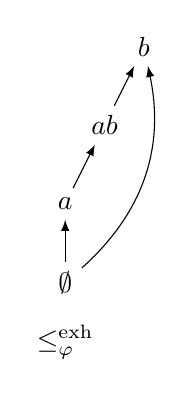
\begin{tikzpicture}
		\node at (0,-0.75){$\le^{\exh}_{\phi}$};
		\node at (0,0)(e){$\emptyset$};
		\node at (0,1)(a){$a$};
		\node at (0.5,2)(ab){$ab$};
		\node at (1,3)(b){$b$};
		\path[-latex]
			(e)edge(a)
			(e)edge[bend right=30](b)
			(a)edge(ab)
			(ab)edge(b);
	\end{tikzpicture}
	\caption{
		The exhaustive $\re$-revealed $\L_{\horn}$-assignment 
		is not guaranteed to be transitive.
	}
	\label{fig:6-hhh-revision-exhaustive-revealed-not-transitive}
\end{figure}

\begin{xmpl}{$\le^{\exh}_{\phi}$ might not be transitive}{6-hhh-revision-exhaustive-revealed-not-transitive}
	Consider an $\HHH$-revision operator $\re$ such that,
	for the set of atoms $\Atoms=\{a,b\}$,
	delivers the following results:
	$[\phi\re\px_{a,ab}]=\{a\}$,
	$[\phi\re\px_{ab,b}]=\{ab\}$
	and
	$[\phi\re\px_{a,b}]=\{\emptyset\}$.
	From this we infer that 
	$a<^{\exh}_{\phi} ab$,
	$ab <^{\exh}_{\phi} b$, 
	$\emptyset <^{\exh}_{\phi} a$
	and 
	$\emptyset <^{\exh}_{\phi} b$.
	These comparisons are depicted in 
	Figure \ref{fig:6-hhh-revision-exhaustive-revealed-not-transitive}.
	In propositional logic we would be able to use 
	postulates $\ppr{5-6}$ to infer from
	the result for $\phi\re\px_{a,ab}$ and for
	$\phi\re\px_{ab,b}$
	that a choice over interpretations $a$, $ab$ and $b$
	has to select $a$;
	based on this, we would infer that the choice over $a$ and $b$
	has to select $a$ as well, meaning that $a$ is considered better 
	than $b$.
	However, in the Horn fragment there is no way of 
	enforcing choice over $a$, $ab$ and $b$,
	since $\{a,b,ab\}$ is not $\horn$-closed.
	This makes it possible for the result to be $\emptyset$
	when revising by $\px_{a,b}$,
	leaving $a$ and $b$ incomparable in $\le^{\exh}_{\phi}$.
\end{xmpl}

Example \ref{ex:6-hhh-revision-exhaustive-revealed-not-transitive}
illustrates one of the consequences of restricting the
language: since there are certain configurations 
of outcomes the agent never gets to see,
the revision operator
becomes less precise at identifying the relationship 
between certain outcomes:
if $w_1\subseteq w_2$ or $w_2 \subseteq w_1$, 
then $\{w_1,w_2\}$ is $\horn$-closed and $\phi\re\px_{1,2}$
behaves as in propositional logic;
but if $w_1$ and $w_2$ are subset-incomparable,
then there is no way to make a comparison only between the two of them,
and the revealed relation may feature patches where
the revision operators has nothing informative to say.

Nevertheless, a glance at
Example \ref{ex:6-hhh-revision-exhaustive-revealed-not-transitive}
suggests an easy fix:
note that the transitive closure of $\le^{\exh}_{\phi}$,
as depicted in Figure \ref{fig:6-hhh-revision-exhaustive-revealed-not-transitive},
is an ordering extension of $\le^{\exh}_{\phi}$, as defined in Section \ref{sec:2-choice-functions},
i.e., a relation that preserves all the comparisons
in $\le^{\exh}_{\phi}$, including the strict ones.
Thus, even if the revision operator does not explicitly state
that $a$ is better than $b$, given the prior information $\phi$,
we may still attempt to infer this from the intermediary comparisons 
of $a<^{\exh}_{\phi} ab$ and $ab <^{\exh}_{\phi} b$.
Importantly, adding the comparison $a <^{\exh}_{\phi} b$
to $\le^{\exh}_{\phi}$ does not misrepresent $\re$: 
the augmented relation underlies the same revision operator.
This raises the hope of a general strategy,
and we will soon see the conditions under which this strategy is successful.

So far, so good.
The problem, as has been already documented \cite{DelgrandeP15,DelgrandePW18},
is that these elements alone are not enough to 
deliver a representation result. 
A first indication that more needs to be done is the fact that
assignments based on standard, distance-based preorders 
(either total or partial, r-faithful or not) 
cannot be used to induce $\HHH$-revision operators.

\begin{figure}\centering
	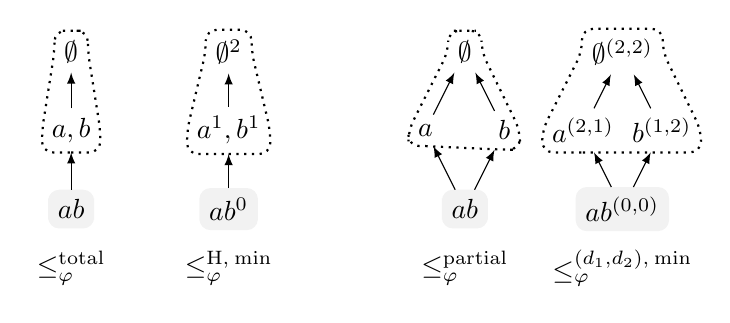
\begin{tikzpicture}
		\node at (0,-0.75){$\le^{\totalPre}_{\phi}$};
		\node at (0,0)(ab){$ab$};
		\node at (0,1)(a){$a,b$};
		\node at (0,2)(e){$\emptyset$};
		\path[-latex]
			(ab) edge (a)
			(a) edge (e);
		\fill[opacity=0.05,rounded corners=4]
			(ab.south)--
			(ab.south west)--
			(ab.west)--
			(ab.north west)--
			(ab.north)--
			(ab.north east)--
			(ab.east)--
			(ab.south east)--
			(ab.south);
		\draw[thick,dotted, rounded corners=4]
			(a.south)--
			(a.south east)--
			(a.east)--
			(e.east)--
			(e.north east)--
			(e.north)--
			(e.north west)--
			(e.west)--
			(a.west)--
			(a.south west)--
			(a.south);


		\node at (2,-0.75){$\le^{\hamming,\:\min}_{\phi}$};
		\node at (2,0)(ab){$ab^{0}$};
		\node at (2,1)(a){$a^{1},b^{1}$};
		\node at (2,2)(e){$\emptyset^{2}$};
		\path[-latex]
			(ab) edge (a)
			(a) edge (e);
		\fill[opacity=0.05,rounded corners=4]
			(ab.south)--
			(ab.south west)--
			(ab.west)--
			(ab.north west)--
			(ab.north)--
			(ab.north east)--
			(ab.east)--
			(ab.south east)--
			(ab.south);
		\draw[thick,dotted, rounded corners=4]
			(a.south)--
			(a.south east)--
			(a.east)--
			(e.east)--
			(e.north east)--
			(e.north)--
			(e.north west)--
			(e.west)--
			(a.west)--
			(a.south west)--
			(a.south);

		\node at (5,-0.75){$\le^{\partialPre}_{\phi}$};
		\node at (5,0)(ab){$ab$};
		\node at (4.5,1)(a){$a$};
		\node at (5.5,1)(b){$b$};
		\node at (5,2)(e){$\emptyset$};
		\path[-latex]
			(ab) edge (a)
			(a) edge (e)
			(ab) edge (b)
			(b) edge (e);
		\fill[opacity=0.05,rounded corners=4]
			(ab.south)--
			(ab.south west)--
			(ab.west)--
			(ab.north west)--
			(ab.north)--
			(ab.north east)--
			(ab.east)--
			(ab.south east)--
			(ab.south);
		\draw[thick,dotted, rounded corners=4]
			(a.south)--
			(b.south)--
			(b.south east)--
			(b.east)--
			(e.east)--
			(e.north east)--
			(e.north)--
			(e.north west)--
			(e.west)--
			(a.west)--
			(a.south west)--
			(a.south);	

		\node at (7,-0.75){$\le^{(\dd_{1},\dd_{2}),\:\min}_{\phi}$};
		\node at (7,0)(ab){$ab^{(0,0)}$};
		\node at (6.5,1)(a){$a^{(2,1)}$};
		\node at (7.5,1)(b){$b^{(1,2)}$};
		\node at (7,2)(e){$\emptyset^{(2,2)}$};
		\path[-latex]
			(ab) edge (a)
			(a) edge (e)
			(ab) edge (b)
			(b) edge (e);
		\fill[opacity=0.05,rounded corners=4]
			(ab.south)--
			(ab.south west)--
			(ab.west)--
			(ab.north west)--
			(ab.north)--
			(ab.north east)--
			(ab.east)--
			(ab.south east)--
			(ab.south);
		\draw[thick,dotted, rounded corners=4]
			(a.south)--
			(b.south)--
			(b.south east)--
			(b.east)--
			(e.east)--
			(e.north east)--
			(e.north)--
			(e.north west)--
			(e.west)--
			(a.west)--
			(a.south west)--
			(a.south);	
	\end{tikzpicture}
	\caption{
		Preorders $\le^{\totalPre}_{\phi}$ and $\le^{\partialPre}_{\phi}$
		for $\phi=a\land b\land\lnot c$ and $\mu=\lnot(a\land b)\land \lnot c$.
		Models of $\phi$ are shaded in gray, 
		models of $\mu$ are surrounded by the 
		dotted line.
		Neither of the preorders
		$\le^{\totalPre}_{\phi}$ and $\le^{\partialPre}_{\phi}$
		delivers a $\horn$-closed set of interpretations,
		and thus cannot be used to model 
		$\HHH$-revision operators.
		These preorders coincide with $\le^{\hamming,\:\min}_{\phi}$
		and $\le^{(\dd_{1},\dd_{2}),\:\min}_{\phi}$,
		as presented in Example \ref{ex:3-revision-dmin}.
	}
	\label{fig:6-hhh-revision-standard-ops-no-good}
\end{figure}

\begin{xmpl}{Preorders that do not induce an $\HHH$-revision operator}{6-hhh-revision-standard-ops-no-good}
	For the set of atoms $\Atoms=\{a,b,c\}$,
	consider formulas $\phi=a\land b\land\lnot c$
	and $\mu=\lnot (a\land b)\land\lnot c$.
	We have that $[\phi]=\{ab\}$ and
	$[\mu]=\{\emptyset,a,b\}$.
	Both $\phi$ and $\mu$ are Horn formulas,
	and are thus valid inputs to an $\HHH$-revision operator.
	Consider, however, a total assignment $\as^{\totalPre}$
	and a partial assignment $\as^{\partialPre}$
	that assigns to $\phi$ 
	the preorders
	$\le^{\totalPre}_{\phi}$ and  $\le^{\partialPre}_{\phi}$,
	respectively,
	both depicted in Figure \ref{fig:6-hhh-revision-standard-ops-no-good}.
	We obtain that:
	\begin{align*}
		\min_{\le^{\totalPre}_{\phi}}[\mu] &=\min_{\le^{\partialPre}_{\phi}}[\mu]\\
											&= \{a,b\},	
	\end{align*}
	and hence $[\phi\re^{\totalPre}\mu]=[\phi\re^{\partialPre}\mu]=\{a,b\}$.
	Since $\cl_{\horn}(\{a,b\})=\{\emptyset,a,b\}\neq\{a,b\}$,
	it follows that 
	$[\phi\re^{\totalPre}\mu]$ and $[\phi\re^{\partialPre}\mu]$ 
	cannot be represented as a Horn formula,
	i.e., the $\as^{\totalPre}$-induced and $\as^{\partialPre}$-induced
	revision operators do not work as 
	$\HHH$-revision operators.

	This finding is significant,
	because $\le^{\totalPre}_{\phi}$
	coincides on the models of $\phi$ and $\mu$ 
	with the preorder generated 
	by many of the distance-based
	assignments we looked at in Section \ref{sec:3-revision}
	(the set of atoms is considered to coincide with $\Atoms$ in that example),
	namely with 
	$\le^{\hamming,\:\min}_{\phi}$,
	$\le^{\hamming,\:\leximin}_{\phi}$,
	$\le^{\hamming,\:\max}_{\phi}$,
	$\le^{\hamming,\:\leximax}_{\phi}$
	and
	$\le^{\hamming,\:\ssum}_{\phi}$.
	Also, $\le^{\partialPre}_{\phi}$
	coincides on the models of $\phi$ and $\mu$
	with the partial preorder $\le^{(\dd_{1},\dd_{2}),\:\min}_{\phi}$
	presented in Example \ref{ex:3-revision-dmin}.
\end{xmpl}

Example \ref{ex:6-hhh-revision-standard-ops-no-good}
shows that, like in Section \ref{sec:6-revision-hph},
there are certain preorders bound to deliver results 
that cannot be recast as Horn formulas.
Unfortunately, these preorders appear in
the distance-based assignments we have introduced
in Section \ref{sec:3-revision} for $\L$-revision operators.
The upshot, then, is that none of these assignments
can be repurposed for $\HHH$-revision.

The problem highlighted by Example \ref{ex:6-hhh-revision-standard-ops-no-good}
is that properties $\oor{1-7}$, by themselves,
make an $\L_{\horn}$-assignment $\as$ on interpretations
ill-equipped to induce a well-defined $\HHH$-revision operator.
The solution, as for $\HPH$-revision operators, 
is to rein in the preorders we are looking at.
The purpose, here, is to find a restriction on 
$\L_{\horn}$-assignments that ensures 
they deliver $\horn$-closed results when the new information is 
a Horn formula.
This is done via the following property, intended to hold for 
any Horn formula $\phi$ and interpretations $w_1$ and $w_2$:

\begin{description}
	\item[($\oor{\HC}$)] For any Horn formula $\mu$, 
		it holds that $\min_{\le_{\phi}}[\mu]$ if $\horn$-closed.
\end{description}

% We will do this in two ways, depending on whether the preorders 
% we are working with are total or partial.

% Total preorders, we know from Section \ref{sec:3-revision},
% go hand in hand with postulates $\ppr{1-6}$, but we are 
% beginning to see that for the Horn fragment these elements 
% may not be enough.

% \begin{description}
% 	\item[($\oor{\TCMPL}$)] 
% 		If $w_1 \approx_{\phi}w_2$, 
% 		then $(w_1\cap w_2) \le_{\phi} w_1$ or $(w_1\cap w_2) \le_{\phi} w_2$.	
% 		% If $w_1 \not<_{\phi}w_2$ and $w_2\not<_{\phi}w_1$, 
% 		% then $(w_1\cap w_2) \in\min_{\le_{\phi}}\cl_{\horn}(\{w_1,w_2\})$.
% \end{description}

\begin{figure}\centering
	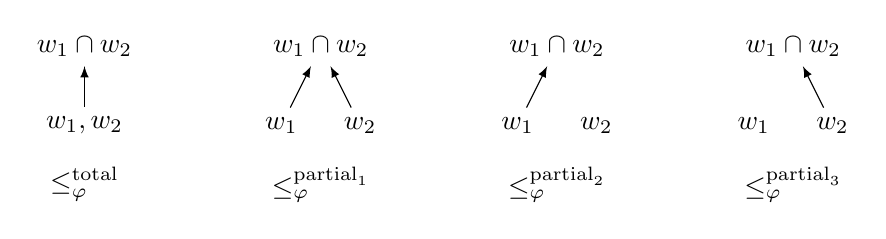
\begin{tikzpicture}
		\node at (0,-0.75)(1){$\le^{\totalPre}_{\phi}$};
		\node at (0,0)(1){$w_1,w_2$};
		\node at (0,1)(2){$w_1\cap w_2$};
		\path[-latex] (1)edge(2);

		\node at (3,-0.75){$\le^{\partialPre_1}_{\phi}$};
		\node at (2.5,0)(1){$w_1$};
		\node at (3.5,0)(2){$w_2$};
		\node at (3,1)(3){$w_1\cap w_2$};
		\path[-latex] (1)edge(3)(2)edge(3);

		\node at (6,-0.75){$\le^{\partialPre_2}_{\phi}$};
		\node at (5.5,0)(1){$w_1$};
		\node at (6.5,0)(2){$w_2$};
		\node at (6,1)(3){$w_1\cap w_2$};
		\path[-latex] (1)edge(3);

		\node at (9,-0.75){$\le^{\partialPre_3}_{\phi}$};
		\node at (8.5,0)(1){$w_1$};
		\node at (9.5,0)(2){$w_2$};
		\node at (9,1)(3){$w_1\cap w_2$};
		\path[-latex] (2)edge(3);
	\end{tikzpicture}	
	\caption{
		Preorders, total and partial, that deliver results that 
		are not $\horn$-closed when revising by a Horn formula $\mu$, 
		with $[\mu]=\{w_1,w_2,w_1\cap w_2\}$.
		It is assumed that $w_1\nsubseteq w_2$ and $w_2\nsubseteq w_1$,
		such that $w_1\cap w_2$ is an interpretation distinct from both $w_1$ and $w_2$.
		The goal of property $\oor{\HC}$ is to prevent the occurrence of these configurations.
	}
	\label{fig:6-hhh-revision-non-compliant-preorders}
\end{figure}

Property $\oor{\HC}$, where `$\HC$' 
stands for \emph{Horn compliance} \cite{DelgrandeP15,DelgrandePW18},
guarantees that the $\le_{\phi}$-minimal elements of $[\mu]$,
when $\mu$ is a Horn formula, can be represented by a Horn formula.
Property $\oom{\HC}$ works for both total and partial preorders,
and its role, essentially, is to rule out situations such as the ones 
in Figure \ref{fig:6-hhh-revision-non-compliant-preorders},
where revision by a Horn formula yields a set of interpretations 
that cannot be expressed as a Horn formula.
% In deference to this fact,
An $\L_{\horn}$-assignment $\as$ on interpretations 
is \emph{Horn compliant} if it satisfies property $\oor{\HC}$.
It is straightforward to see that
property $\oor{\HC}$ is a condition that is both necessary and sufficient
for a propositional revision operator to function as an $\HHH$-revision operator.


% Property $\oor{\TCMPL}$, where `$\TCMPL$' denotes \emph{triples compliance},
% says that if interpretations $w_1$ and $w_2$ are equally good in $\le_{\phi}$,
% then $w_1\cap w_2$ should also be considered as least as good as $w_1$ and $w_2$.
% If $w_1 \subseteq w_2$ or $w_2 \subseteq w_1$, then property $\oor{\TCMPL}$
% is trivially satisfied, but if $w_1$ and $w_2$ are subset-incomparable,
% then property $\oor{\TCMPL}$ is more meaningful and its role, essentially,
% is to eliminate the configuration in Figure \ref{fig:6-hhh-revision-non-compliant-preorders}.
% The intuition behind this requirement is that if
% $w_1$ and $w_2$ are subset-incomparable,
% then the choice over $\{w_1,w_2,w_1\cap w_2\}$
% cannot consist of $w_1$ and $w_2$ alone,
% since this can yield a revision result that is not $\horn$-closed.
% Thus, property $\oor{\TCMPL}$ forces that the
% choice over interpretations $\{w_1,w_2,w_1\cap w_2\}$
% contains the interpretation $w_1\cap w_2$ as well,
% guaranteeing a $\horn$-closed result.
% The guiding intuition is that if 
% The solution, then, is to ensure that the preorder $\le_{\phi}$ is never 
% in a situation where $w_1$ and $w_2$ can occur as the minimal elements in 
% $\cl_{\horn}(\{w_1,w_2\})$.

% Property $\oor{\TCMPL}$ looks convoluted because it packs just as much information 
% as needed to work for both partial and total preorders.
% We can unpack it into a more understandable format
% if we look at the configurations it is indended to prevent.
% If $\le_{\phi}$ is assumed to be a total preorder, then the precondition 
% in property $\oor{\TCMPL}$ becomes equivalent to saying that $w_1\approx_{\phi} w_2$
% and $\oor{\TCMPL}$, as a whole, boils down to the following property, 
% holding for any Horn formula $\phi$ and interpretations $w_1$ and $w_2$:

% \begin{description}
% 	\item[($\oor{\TCMPL_\totalPre}$)] If $w_1 \approx_{\phi}w_2$, 
% 		then $(w_1\cap w_2) \le_{\phi} w_1$ or $(w_1\cap w_2) \le_{\phi} w_2$.
% \end{description}



% In other words, property $\oor{\TCMPL_\totalPre}$ eliminates the 
% configuration depicted by $\le^{\totalPre}_{\phi}$ 
% in Figure \ref{fig:6-hhh-revision-non-compliant-preorders},
% in which $\min_{\le^{\totalPre}_{\phi}}\{w_1,w_2,w_1\cap w_2\}=\{w_1,w_2\}$.
% Note that $\{w_1,w_2\}$ is not $\horn$-closed,
% and is therefore not a viable result for an $\HHH$-revision operator.

% If $\le_{\phi}$ is assumed to be partial, then property $\oor{\TCMPL}$
% eliminates the configurations depicted by 
% $\le^{\partialPre_1}_{\phi}$,
% $\le^{\partialPre_2}_{\phi}$
% and
% $\le^{\partialPre_3}_{\phi}$
% in Figure \ref{fig:6-hhh-revision-non-compliant-preorders}.
% In all three of these cases it holds that 
% $\min_{\le^{\partialPre_i}_{\phi}}\{w_1,w_2,w_1\cap w_2\}=\{w_1,w_2\}$,
% for $i\in\{1,2,3\}$,
% and it is in our interest to prevent such configurations from occurring.
% Note that the problematic cases all involve pairs of interpretations 
% $w_1$ and $w_2$ that are subset-incomparable, 
% and cannot therefore be represented precisely by a Horn formula. 
% If $w_1 \subseteq w_2$ or $w_2 \subseteq w_1$, then property $\oor{\TCMPL}$ is trivially true.

% Property $\oor{\TCMPL}$ is formulated for pairs $\{w_1,w_2\}$ of interpretations
% and makes sure that a choice 

% However, our intention is to cover any $\horn$-closed 
% set $\W$ of interpretations, in order to ensure that its $\le_{\phi}$-minimal 
% elements can represent a Horn formula: 
% the idea here is that we want to foolproof $\le_{\phi}$ such that, 
% whatever the new information $\mu$ is, 
% the result $\min_{\le_\phi}[\mu]$ of revision 
% by $\mu$ can be recast as a Horn formula.
% If $\le_{\phi}$ is a total preorder, 
% property $\oor{\TCMPL}$ allows us to do that.

% \begin{prp}{}{6-hhh-revision-triples-horn-compliance}
% 	If $\le_{\phi}$ is a total preorder, then 
% 	$\le_{\phi}$ satisfies property $\oor{\TCMPL}$
% 	if and only if, 
% 	for any Horn formula $\mu$,
% 	it holds that $\min_{\le_{\phi}}[\mu]$ is $\horn$-closed.
% \end{prp}
% \begin{prf*}{}{}%
% 	(``$\Rightarrow$'')
% 	Suppose $\le_{\phi}$ satisfies property $\oor{\TCMPL}$
% 	and $min_{\le_{\phi}}[\mu]$ is not $\horn$-closed.
% 	Then there exist interpretations 
% 	$w_1$ and $w_2$ in $\min_{\le_{\phi}}[\mu]$ such that 
% 	$w_1\cap w_2\notin\min_{\le_{\phi}}[\mu]$.
% 	Since $\le_{\phi}$ is total, this implies that $w_1\approx_{\phi}w_2<_{\phi}w_1\cap w_2$,
% 	which contradicts property $\oor{\TCMPL}$.

% 	(``$\Leftarrow$'')
% 	Take two interpretations $w_1$ and $w_2$ such that $w_1\approx_{\phi}w_2$,
% 	and an $\L_{\horn}$-proxy $\px_{1,2}$ of $\{w_1,w_2\}$.
% 	We obtain that $\min_{\le_{\phi}}\px_{1,2}$ is $\horn$-closed,
% 	which implies that $w_1\cap w_2\in \min_{\le_{\phi}}\px_{1,2}$,
% 	i.e., $w_1\cap w_1\le_{\phi}w_1$.
% \end{prf*}


% \begin{thm}{}{6-hhh-revision-equiv-TCMPL}
% 	If $\re$ is an $\L$-revision operator
% 	and $\as$ is an $\L$-assignment on interpretations
% 	that represents it,
% 	then $\re$ is an $\HHH$-revision operator, 
% 	when restricted to Horn formulas,
% 	if and only if $\as$ satisfies property $\oor{\TCMPL}$,
% 	when restricted to Horn formulas.
% \end{thm}
% \begin{prf*}{}{}%
% 	We have that $\re$ being an $\HHH$-revision operator
% 	is equivalent to 
% 	$\min_{\le_{\phi}}[\mu]$ being $\horn$-closed,
% 	for any Horn formulas $\phi$ and $\mu$,
% 	which, using Proposition \ref{prop:6-hhh-revision-triples-horn-compliance},
% 	is equivalent to property $\oor{\TCMPL}$ being satisfied.
% \end{prf*}


% Horn compliance, however, :
% it guarantees that the result of an 
% $\as$-induced revision operator can be expressed 
% as a Horn formula,
% and that only such assignments can represent 
% $\HHH$-revision operators,
% but it does not ensure 
% that such formulas have other 
% desirable properties.
% We will see that these properties can be 
% guaranteed by adding on properties $\oor{1-7}$.

With the expressibility issue fixed, the next step is to 
look at the effect of postulates $\ppr{1-6}$, or $\ppr{1-5}$ and $\ppr{7-8}$,
and connect them to properties $\oor{1-7}$.
However, another problem rears its head:
it turns out that restricted to Horn formulas, 
the revision postulates 
end up saying less than their propositional counterparts,
to the point where they can now induce
unwanted assignments. 
To understand this issue, it is best to 
look at total and partial preorders separately.

\subsubsection{Total preorders}
Total preorders, we know from Section \ref{sec:3-revision},
go hand in hand with postulates $\ppr{1-6}$, but we are 
beginning to see that for the Horn fragment these elements 
may not be enough.
As has been observed, one outstanding problem is the 
presence of non-transitive cycles in assignments 
that can represents $\HHH$-revision operators
that satisfy postulates $\ppr{1-6}$.

\begin{figure}\centering
	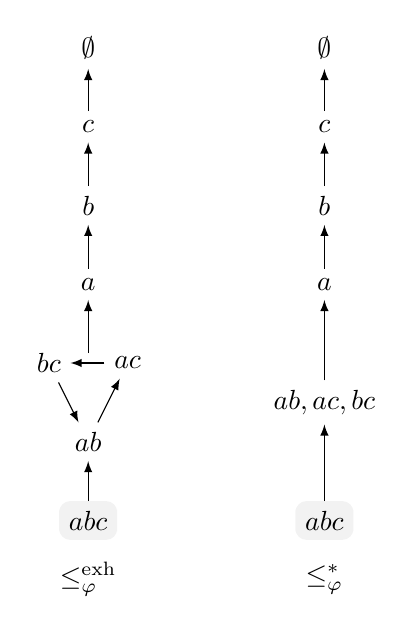
\begin{tikzpicture}
		\node at (0,-0.75){$\le^{\exh}_{\phi}$};
		\node at (0,0)(abc){$abc$};
		\node at (0,1)(ab){$ab$};
		\node at (0.5,2)(ac){$ac$};
		\node at (-0.5,2)(bc){$bc$};
		\node at (0,2)(anchor1){};
		\node at (0,3)(a){$a$};
		\node at (0,4)(b){$b$};
		\node at (0,5)(c){$c$};
		\node at (0,6)(e){$\emptyset$};
		\path[-latex]
		(abc) edge (ab)
		(ab) edge (ac)
		(ac) edge (bc)
		(bc) edge (ab)
		(anchor1) edge (a)
		(a) edge (b)
		(b)edge(c)
		(c)edge(e);		
	\fill[opacity=0.05,rounded corners=4]
		(abc.south)--
		(abc.south west)--
		(abc.west)--
		(abc.north west)--
		(abc.north)--
		(abc.north east)--
		(abc.east)--
		(abc.south east)--
		(abc.south);

	\node at (3,-0.75){$\le^{\ast}_{\phi}$};
	\node at (3,0)(abc){$abc$};
	\node at (3,1.5)(ab){$ab,ac,bc$};
	\node at (3,3)(a){$a$};
	\node at (3,4)(b){$b$};
	\node at (3,5)(c){$c$};
	\node at (3,6)(e){$\emptyset$};
	\path[-latex]
		(abc) edge (ab)
		(ab) edge (a)
		(a) edge (b)
		(b)edge(c)
		(c)edge(e);		
	\fill[opacity=0.05,rounded corners=4]
		(abc.south)--
		(abc.south west)--
		(abc.west)--
		(abc.north west)--
		(abc.north)--
		(abc.north east)--
		(abc.east)--
		(abc.south east)--
		(abc.south);
	\end{tikzpicture}
	\caption{
		The exhaustive revealed ranking $\le^{\exh}_{\phi}$
		for an $\HHH$-revision operator $\re$ that satisfies
		postulates $\ppr{1-5}$ and $\ppr{7-8}$
		and $\phi=a\land b\land c$,
		together with the ranking $\le^{\ast}_{\phi}$
		obtained as the transitive closure of $\le^{\exh}_{\phi}$.
		The ranking $\le^{\exh}_{\phi}$
		contains a non-transitive 
		cycle between $ab$, $ac$ and $bc$,
		and behaves like a total preorder otherwise.
		The non-transitive cycle goes undetected 
		when $\re$ processes 
		only Horn formulas.
		The transitive closure $\le^{\ast}_{\phi}$
		of $\le^{\exh}_{\phi}$
		fixes the non-transitivity issue but
		does not represent the revision operator $\re$
		anymore.
		}
	\label{fig:6-hhh-revision-cycle}
\end{figure}

\begin{xmpl}{\cite{DelgrandeP15,DelgrandePW18}}{6-hhh-revision-cycles}
	For the set of atoms $\Atoms=\{a,b,c\}$
	and the formula $\phi=a\land b\land c$,	
	consider an $\HHH$-revision operator $\re$
	that induces the exhaustive revealed plausibility
	relation $\le^{\exh}_{\phi}$ in Figure \ref{fig:6-hhh-revision-cycle}.
	In other words, it holds that 
	$[\phi\re\px_{ab,ac}]=\{ab\}$,
	$[\phi\re\px_{ac,bc}]=\{ac\}$,
	$[\phi\re\px_{bc,ab}]=\{bc\}$,
	and so on:
	the results of the revision operator on
	all the possible inputs can be read off 
	from Figure \ref{fig:6-hhh-revision-cycle}.

	The significant detail about the 
	revealed relation $\le^{\exh}_{\phi}$
	is that it 
	behaves like a total preorder everywhere 
	except on $ab$, $ac$ and $bc$,
	which are fixed into a non-transitive cycle.
	In other words, $\re$ decides
	that $ab <^{\exh}_{\phi} ac <^{\exh}_{\phi} bc <^{\exh}_{\phi} ab$,
	which implies that $\le_{\phi}$ does not satisfy property $\oor{3}$
	on $ab$, $ac$ and $bc$.

	We would expect that the failure of $\le^{\exh}_{\phi}$ to 
	satisfy property $\oor{3}$
	translates into $\re$ 
	not satisfying some of the revision postulates:
	and if we were working in propositional logic,
	this would indeed be the result.
	In propositional logic we can always revise by a 
	propositional formula
	that has exactly $ab$, $ac$ and $bc$ as its models;
	revision with this formula 
	together with postulate $\ppr{3}$ 
	implies that $\min_{\le^{\exh}_{\phi}}\{ab,ac,bc\}$
	has to be non-empty,
	contrary to the present situation:
	in the framework of propositional logic 
	the regular postulates $\ppr{1-6}$ make 
	a revision operator such as the operator $\re$ specified here 
	impossible.

	Interestingly, in the Horn fragment the operator $\re$
	turns out to be a perfectly legal $\HHH$-revision operator:
	it can be checked that $\re$ satisfies postulates $\ppr{1-6}$
	\cite{DelgrandeP15,DelgrandePW18}.
	The reason why the cycle manages to slip through undetected
	is that in the Horn fragment there is no formula
	that has exactly $ab$, $ac$ and $bc$ as its models,
	since $\{ab,ac,bc\}$ is not $\horn$-closed.
	The closest we can come to this is by 
	using an $\L_{\horn}$-proxy 
	$\px_{ab,ac,bc}$ of $\{ab,ac,bc\}$,
	but $[\px_{ab,ac,bc}]=\cl_{\horn}(\{ab,ac,bc\})=\{\emptyset,a,b,c,ab,ac,bc\}$,
	and simply asking 
	that $\min_{\le^{\exh}_{\phi}}[\px_{ab,ac,bc}]$ is non-empty 
	does not prevent the cycle.
	
	A tentative fix for this situation is to 
	replace $\le^{\exh}_{\phi}$,
	as in Example \ref{ex:6-hhh-revision-exhaustive-revealed-not-transitive}	
	with its transitive closure $\le^{\ast}_{\phi}$,
	also depicted in Figure \ref{fig:6-hhh-revision-cycle}.
	This has the effect of flattening the cycle
	by introducing indifference between $ab$, $bc$ and $ac$.
	The downside of this move however, is that $\le^{\ast}_{\phi}$
	does not preserve the information provided by $\re$:
	we can see this by looking at the revision operator $\re^{\ast}$ induced 
	by the preorder $\le^{\ast}_{\phi}$, 
	and comparing it to $\re$: 
	we have that
	$[\phi\re\px_{ab,ac}]=\{ab\}$,
	i.e.,
	$\min_{\le^{\exh}_{\phi}}\{ab,ac,a\} = \{ab\}$,
	whereas 
	$\min_{\le^{\ast}_{\phi}}\{ab,ac,a\} = \{ab,ac\}$,
	i.e., 
	$[\phi\re^{\ast}\px_{ab,ac}]=\{ab,ac\}$.
	The cycle-free transitive closure of $\le^{\exh}_{\phi}$
	represents a different revision operator, 
	one that does not even return a Horn formula!

	The moral here is that 
	the preorder $\le^{\exh}_{\phi}$
	depicted in Figure \ref{fig:6-hhh-revision-cycle}
	cannot be extended to a total preorder while
	still remaining faithful to the revision operator $\re$:
	eliminating the cycle between $ab$, $bc$ and $ac$
	would lead to $\le^{\exh}_{\phi}$ misrepresenting $\re$.
	% Note that the cycle is obtained even if we use the 
	% exclusive $\re$-revealed assignment instead of the
	% exhaustive one.
	The cycle, here, is unavoidable.
\end{xmpl}

In Example \ref{ex:6-hhh-revision-exhaustive-revealed-not-transitive}
we encountered an exhaustive $\HHH$-revision operator 
that induced a non-transitive ranking on outcomes,
but this ranking could be made transitive by 
filling in the gaps with the
comparisons inferred by transitivity.
Example \ref{fig:6-hhh-revision-cycle}
shows that there are exhaustive $\HHH$-revision operators 
inducing rankings that are not only non-transitive,
but that cannot even be made transitive:
postulates $\ppr{1-6}$,
the most demanding revision postulates we have,
not only fail to notice the cycle between $ab$, $ac$ and $bc$,
but allow the agent to revise in a way that makes the cycle
compulsory.
This is a direct result of the Horn fragment's inability
to capture certain sets of interpretations:
whereas in propositional logic we would be able 
to leverage postulates $\ppr{1-6}$
to make sure that the revealed exhaustive ranking is transitive,
in the Horn fragment this move is not possible.

% Example \ref{fig:6-hhh-revision-cycle} 
% throws a wrench in the works:
% $\HHH$-revision operators exist for which this is not possible,
% i.e., that cannot be rationalized by transitive plausibility relations.
% In propositional logic 
% such operators are disallowed by postulates $\ppr{1-6}$,
% but in the Horn fragment the same postulates fail 
% to provide the same guarantees.

% Does this mean that there is no guarantee that 
% revision for Horn formulas can be rationalized in a 
% meaningful way?

One way to deal with this situation is to make sure that 
an exhaustive $\HHH$-revision operator does not 
revise in a way that paints it into a non-transitive corner,
and it is here that the literature on rational choice proves useful,
as it suggests a tool of proven efficacy: Suzumura consistency.
Recall Theorem \ref{thm:2-suzumura-consistency},
saying that Suzumura consistency 
is both a necessary and sufficient condition for a binary relation to
have an extension that is a total preorder.
In the context of revision, we can formulate Suzumura consistency
as a property that applies to preorders in an assignment $\as$ on interpretations.
Thus, for any 
Horn formula $\phi$
and interpretations $w_1$, \dots, $w_n$, 
the property is as follows:

\begin{description}
	\item[($\oor{\SCON}$)] If $w_1 \le_{\phi}\dots \le_{\phi}w_n$,
		then $w_{n}\not<_{\phi} w_{1}$.
\end{description}

Property $\oor{\SCON}$, 
with $\SCON$ standing for \emph{Suzumura consistency},
has a natural reading: 
if $w_1$ is at least as good as $w_2$ according to $\le_\phi$,
$w_2$ is at least as good as $w_3$,
and so on, all the way to $w_n$, then
the betterness of $w_1$ should propagate down the line,
i.e., the last outcome in this sequence cannot 
be strictly better than $w_1$.
Property $\oor{\SCON}$ is, of course, implied by transitivity,
i.e., by property $\oor{3}$,
but if property $\oor{3}$ cannot be enforced then $\oor{\SCON}$
is the safest bet, as long as $\oor{\SCON}$ itself can be enforced.

How can we make sure that $\HHH$-revision operators 
describe only Suzumura consistent preorders? 
By supplementing the standard set of postulates
with a special postulate, tailored specifically for property $\oor{\SCON}$.
% Before going ahead with this strategy, a few observations are required.
% First, the additional postulate is meant to ensure that the assignment inferred 
% from the revision operator $\re$, and intended to 
% represent $\re$, satisfies property $\oor{\SCON}$:
% it turns out, however, that it matters how the assignment is inferred,
% i.e., whether it is the exhaustive or exclusive. 
% Since the exhaustive assignment is used when the base set postulates is $\ppr{1-6}$
% and the exclusive assignment is used for postulates $\ppr{1-5}$ and $\ppr{7-8}$,
% we will need two postulates, one for each case.
We will formulate the postulate using 
the notion of an $\L_{\horn}$-proxy
of a set $\W$ of interpretations, 
introduced in Section \ref{sec:6-horn-fragment}: 
recall, this is a Horn formula $\px_{\W}$
such that $[\px_{\W}]=\cl_{\horn}(\W)$.
We will apply this notion to singletons $\{w_i\}$ 
and pairs $\{w_i,w_j\}$ of interpretations,
in which case we write $\px_{i}$ and $\px_{i,j}$
instead of $\px_{w_i}$ and $\px_{w_i,w_j}$, respectively.
Since singleton sets of interpretations are $\horn$-closed,
it holds that $[\px_{i}]=\cl_{\horn}(\{w_i\})=\{w_i\}$.
Pairs of interpretations are not necessarily $\horn$-closed,
in which case $[\px_{i,j}]$ may contain
the additional interpretation $w_i\cap w_j$.

The additional postulate, or, more precisely, 
postulate schema, is intended 
to work for the exhaustive revealed assignment,
and meant to apply for any Horn formula $\phi$, integer $n$,
interpretations $w_1$, \dots, $w_n$
and their associate $\L_{\horn}$-proxy formulas:

\begin{description}
	\item[($\ppr{\SCON}$)]
		If 
			$(\phi\re\px_{1,2})\land\px_{1}$ is consistent,
			\dots,
			$(\phi\re\px_{n-1,n})\land\px_{n-1}$ is consistent,
		then it does not hold that both
		$(\phi\re\px_{n,1})\land\px_{n}$ is consistent
		and that $(\phi\re\px_{n,1})\land\px_{1}$ is inconsistent.
\end{description}

Postulate $\ppr{\SCON}$ expresses the same idea as property $\oor{\SCON}$,
but using formulas and the revision operator 
instead of interpretations and the preorder.
Note that this connection applies only if the preorder
is part of the exhaustive $\re$-revealed assignment.

\begin{thm}{}{6-SCON-scon}
	If $\re$ is an $\HHH$-revision operator 
	and $\as^{\exh}$ is the $\re$-revealed exhaustive assignment, then
	$\re$ satisfies postulate $\ppr{\SCON}$
	if and only if 
	$\as^{\exh}$ satisfies property $\oor{\SCON}$.
\end{thm}
\begin{prf*}{}{}%
	(``$\Rightarrow$'')
	Assume $\re$ satisfies postulate $\ppr{\SCON}$ and 
	take interpretations $w_1$, \dots, $w_n$
	such that $w_1 \le^{\exh}_{\phi}\dots \le^{\exh}_{\phi} w_n$,
	and suppose $w_n<^{\exh}_{\phi}w_1$.
	It follows, first, that $w_1\in[(\phi\re\px_{1,2})\land\px_{1}]$,
	\dots, $w_{n-1}\in[(\phi\re\px_{n-1,n})\land\px_{n-1}]$,
	which shows that the precondition of postulate $\ppr{\SCON}$
	is satisfied.
	The assumption that $w_n<^{\exh}_{\phi}w_1$ implies that 
	$[(\phi\re\px_{n,1})\land\px_{n}]=\{w_n\}$,
	i.e., that 
	$(\phi\re\px_{n,1})\land\px_{n}$ is consistent
	and $(\phi\re\px_{n,1})\land\px_{1}$ is inconsistent,
	which is a contradiction.

	(``$\Leftarrow$'')
	Suppose $(\phi\re\px_{1,2})\land\px_{1}$ is consistent,
	\dots, 
	$(\phi\re\px_{n-1,n})\land\px_{n-1}$ is consistent,
	and, in addition, that 
	$(\phi\re\px_{n,1})\land\px_{n}$ is consistent
	and that $(\phi\re\px_{n,1})\land\px_{1}$ is inconsistent.
	It follows from this that 
	$w_1 \le^{\exh}_{\phi}\dots\le^{\exh}_{\phi} w_n$, and $w_n <^{\exh}_{\phi} w_1$;
	assuming that $\as^{\exh}$ satisfies property $\oor{\SCON}$,
	this leads to a contradiction.
\end{prf*}

It must be mentioned that $\ppr{\SCON}$ is no more than
a rewriting of the acyclicity postulate
that has already been shown to work 
alongside property $\oor{\SCON}$ 
in axiomatizing $\HHH$-revision operators,
while following from postulates $\ppr{1-6}$ in 
propositional logic 
\cite{DelgrandeP15,DelgrandePW18}.
What the current discussion adds is only some context from rational choice theory, 
which allows us to see the existing results in a different light.
Thus, Theorem \ref{thm:6-SCON-scon} shows that 
adding postulate $\ppr{\SCON}$ guarantees
that the preorders in the exhaustive revealed assignment are Suzumura consistent,
and therefore, by Theorem \ref{thm:2-suzumura-consistency}, 
can be extended to a total preorder: 
postulate $\ppr{\SCON}$, in other words, eliminates the cycles
such as the one in Example \ref{ex:6-hhh-revision-cycles},
and is exactly the property we need to make sure that 
the exhaustive revealed preorder can still be 
extended to a total preorder.
This is important for the prospects of a representation theorem:
recall that our goal is to show that $\HHH$-revision operators 
satisfying postulates $\ppr{1-6}$
can be represented using total assignments on interpretations:
with postulate $\ppr{\SCON}$, the exhaustive revealed assignment
can be seen to be a promising candidate, 
since it manages to represent $\re$ and admits of ordering extensions.
Significantly, existing work \cite{DelgrandeP15} 
shows how to construct such an ordering. 
This procedure starts by extending $\le^{\exh}_{\phi}$ to its transitive closure, 
which, by design, guarantees transitivity.
However, the transitive closure is still not guaranteed to be total,
and the construction further contains a way of resolving 
incomparabilities in a way that does not disturb the minimal models of 
any Horn formula $\mu$. The last step is important, 
since it ensures that the extension still manages to represent
the operator $\re$.
This construction, therefore, is at the heart of the following representation 
theorem for $\HHH$-revision operators.

\begin{thm}{\cite{DelgrandeP15}}{6-hhh-revision-total-repr}
	An $\HHH$-revision operator $\re$ satisfies postulates $\ppr{1-6}$ and $\ppr{\SCON}$
	if and only if there exists
	an $\L_{\horn}$-assignment $\as$ on interpretations
	that satisfies properties $\oor{1-7}$ and $\oor{\HC}$
	(i.e., is total, syntax independent, r-faithful and Horn compliant)
	and that represents the operator $\re$.
\end{thm}

What we can add here to this result is the observation that, indeed,
\emph{any} ordering extension of the $\re$-revealed exhaustive assignment
is guaranteed to work.
Let us unpack this statement by taking stock of where we are at this point.
Recall that, if $\phi$ is a Horn formula, 
the exhaustive revealed ranking $\le^{\exh}_{\phi}$ is not guaranteed to be total, 
even with postulates $\ppr{1-6}$ in place:
if $w_1$ and $w_2$ are subset-incomparable interpretations, then they can end up being incomparable
in $\le^{\exh}_{\phi}$ if $[\phi\re\px_{1,2}]=\{w_1\cap w_2\}$,
where $\px_{1,2}$ is an $\L_{\horn}$-proxy of $\{w_1,w_2\}$,
i.e., a Horn formula such that $[\px_{1,2}]=\{w_1,w_2,w_1\cap w_2\}$.
What is more, subset-incomparable intepretations are the \emph{only} 
pairs of interpretations that can end up being incomparable in $\le^{\exh}_{\phi}$:
if $w_1\subseteq w_2$ or $w_2\subseteq w_1$, then 
the $\HHH$-revision operator $\re$ can compare $w_1$ and $w_2$ directly,
and it holds that $w_1 \le^{\exh}_{\phi}w_2$ or $w_2 \le^{\exh}_{\phi}w_1$.
At the same time, because of postulate $\ppr{\SCON}$, $\le^{\exh}_{\phi}$ 
is guaranteed to satisfy property $\oor{\SCON}$.
Thus, by Theorem \ref{thm:2-suzumura-consistency}, 
this means that there exists an ordering extension
of $\le^{\exh}_{\phi}$, 
i.e., a total preorder that preserves all comparisons in $\le^{\exh}_{\phi}$,
including, significantly, the strict ones.
What we can show now is that any such ordering extension 
leaves the minimal elements of any Horn formula $\mu$ unchanged.

\begin{prp}{}{6-hhh-revision-any-ordering-extension}
	If $\re$ is an $\HHH$-revision operator that satisfies postulates $\ppr{1-6}$ and $\ppr{\SCON}$
	and $\phi$ is a Horn formula, 
	then any ordering extension $\le^{\exh\ast}_{\phi}$ of the ranking $\le^{\exh}_{\phi}$ 
	assigned to $\phi$ by the $\re$-revealed exhaustive assignment $\as^{\exh}$
	is such that 
	$\min_{\le^{\exh}_{\phi}}[\mu]=\min_{\le^{\exh\ast}_{\phi}}[\mu]$,
	for any Horn formula $\mu$.
\end{prp}
\begin{prf*}{}{}%
	(``$\subseteq$'')
	Take $w_1\in\min_{\le^{\exh}_{\phi}}[\mu]$ and suppose 
	that $w_1\notin\min_{\le^{\exh\ast}_{\phi}}[\mu]$.
	This means that there exists an interpretation $w_2\in[\mu]$
	such that $w_2<^{\exh\ast}_{\phi}w_1$. 
	Let us reflect, now on what the situation of $w_1$ and $w_2$ can be in $\le^{\exh}_{\phi}$.
	Since $\le^{\exh\ast}_{\phi}$ is an ordering extension of $\le^{\exh}_{\phi}$,
	it cannot be the case that $w_1\le^{\exh}_{\phi}w_2$, since this would imply that 
	$w_1\le^{\exh\ast}_{\phi}w_2$.
	The only possibilities, therefore, are either that $w_2 <^{\exh}_{\phi}w_1$,
	or $w_1$ and $w_2$ are incomparable in $\le^{\exh}_{\phi}$.
	The case where $w_2 <^{\exh}_{\phi}w_1$ contradicts the assumption that $w_1\in\min_{\le^{\exh}_{\phi}}[\mu]$.
	But if $w_1$ and $w_2$ are incomparable in $\le^{\exh}_{\phi}$,
	then it must be the case that $w_1$ and $w_2$ are subset incomparable
	and $[\phi\re\px_{1,2}]=\{w_1\cap w_2\}$.
	Using postulates $\ppr{1-6}$ we now show, as we have done before,
	that it also holds that $\phi\re\px_{w_1,w_1\cap w_2}=\{w_1\cap w_2\}$, 
	which then implies that $(w_1\cap w_2) <^{\exh}_{\phi}w_1$. 
	But, since $w_1$ and $w_2$ are models of $\mu$ and $\mu$ is a Horn formula,
	it follows that $(w_1\cap w_2)\in[\mu]$.
	These facts, now, create a contradiction with the 
	assumption that $w_1\in\min_{\le^{\exh}_{\phi}}[\mu]$.

	(``$\supseteq$'')
	Take $w_1\in\min_{\le^{\exh\ast}_{\phi}}[\mu]$ and 
	suppose that $w_1\notin\min_{\le^{\exh}_{\phi}}[\mu]$.
	This implies that there exists $w_2\in[\mu]$
	such that $w_2<^{\exh}_{\phi}w_1$.
	But, since $\le^{\exh\ast}_{\phi}$ is an ordering extension of $\le^{\exh}_{\phi}$,
	this implies that $w_2<^{\exh\ast}_{\phi}w_1$,
	which leads to a contradiction.
\end{prf*}

Proposition \ref{prop:6-hhh-revision-any-ordering-extension} makes the same point
as the one made by Theorem \ref{thm:6-hhh-revision-total-repr},
but through the vehicle of Suzumura consistency, and provides 
another example of how rational choice can be of use to belief change.

\subsubsection{Partial preorders}
What happens if we replace postulate $\ppr{6}$
with the weaker postulates $\ppr{7-8}$?
Experience teaches us that we should expect partial preorders
represented via the exclusive revealed assignment.
Switching to the Horn fragment complicates things,
of course, but we can use Theorem \ref{thm:6-hhh-revision-total-repr} as a model
for what $\HHH$-revision for exclusive operators should look like.
Example \ref{ex:6-hhh-revision-standard-ops-no-good} shows that 
we need Horn compliance, on the semantic side,
to make sure that an assignment on interpretations 
can represent an $\HHH$-revision operator.
And the case of exhaustive operators teaches us that
another important detail is finding a revealed ranking on outcomes
that can be extended to a transitive preorder,
and that can be elicited using the postulates on hand.

In getting the relationship between the postulates 
and the ranking on outcomes right,
the basic step is inferring the ranking on two interpretations.
For exclusive operators, i.e., operators 
that satisfiy postulates $\ppr{1-5}$ and $\ppr{7-8}$,
the following lemma will prove crucial.

\begin{lem}{}{6-hhh-revision-choice-min}
	If $\re$ is an $\HHH$-revision operator that 
	satisfies postulates $\ppr{1-5}$ and $\ppr{7-8}$
	then, for any interpretations $w_1$ and $w_2$
	and an $\L_{\horn}$-proxy $\px_{1,2}$ of $\{w_1,w_2\}$,
	it holds that $w_1 \in [\phi\re\px_{1,2}]$
	if and only if $w_1\in\min_{\le^{\exc}_{\phi}}\cl_{\horn}(\{w_1,w_2\})$.
\end{lem}
\begin{prf*}{}{}%
	It is straightforward to 
	see that the statement holds if $w_1=w_2$.
	If $w_1\neq w_2$ and 
	$\{w_1,w_2\}$ is $\horn$-closed,
	i.e., $w_1\subseteq w_2$ or $w_2 \subseteq w_1$,
	then $[\px_{1,2}]=\{w_1,w_2\}$,
	and the fact that $w_1 \in [\phi\re\px_{1,2}]$
	is equivalent to the fact that either 
	$w_1 <^{\exc}_{\phi} w_2$, 
	in case $w_2\notin[\phi\re\px_{1,2}]$,
	or that $w_1$ and $w_2$ are incomparable with respect to 
	$\le^{\exc}_{\phi}$,
	in case $w_2\in[\phi\re\px_{1,2}]$.
	In either case, this is equivalent to $w_1$
	being in $\min_{\le^{\exc}_{\phi}}\cl_{\horn}(\{w_1,w_2\})$.

	For the rest of the proof we will then assume that
	$w_1\nsubseteq w_2$ and $w_2\nsubseteq w_1$,
	which implies that 
	$[\px_{1,2}]=\{w_0,w_1,w_2\}$,
	where $w_0 = w_1\cap w_2$.

	(``$\Rightarrow$'')
	Suppose $w_1 \in [\phi\re\px_{1,2}]$
	and
	$w_1\notin\min_{\le^{\exc}_{\phi}}\cl_{\horn}(\{w_1,w_2\})$.
	The latter fact implies that there exists an interpretation in 
	$\cl_{\horn}(\{w_1,w_2\})$ that is strictly better than $w_1$,
	i.e.,  
	$w_2 <^{\exc}_{\phi} w_1$
	or 
	$w_0 <^{\exc}_{\phi} w_1$.
	We show, by a case analysis, that this leads to a contradiction.

	\emph{Case 1}.
	If $w_2 <^{\exc}_{\phi} w_1$,
	then by the definition of the exclusive revealed assignment
	we have that $w_1\notin[\phi\re\px_{1,2}]$,
	which is a contradiction.
	
	\emph{Case 2}.
	If $w_0 <^{\exc}_{\phi} w_1$,
	then, again, by the definition of the exclusive revealed assignment,
	we have that $w_1\notin [\phi\re\px_{0,1}]$.
	However, we also have that:
	\begin{align*}
		(\phi\re\px_{1,2})\land\px_{0,1}&
		\models\phi\re(\px_{1,2}\land\px_{0,1})&
		\text{by}~\ppr{5}\\
						&
		\equiv\phi\re\px_{0,1}.&\text{by}~\ppr{4}
	\end{align*}
	Since $w_1\in[\phi\re\px_{1,2}]$ and $w_1\in[\px_{0,1}]$,
	this implies that $w_1\in[\phi\re\px_{0,1}]$
	and we have thus arrived at a contradiction.

	(``$\Leftarrow$'')
	Suppose 
	$w_1\in\min_{\le^{\exc}_{\phi}}\cl_{\horn}(\{w_1,w_2\})$.
	and
	$w_1 \notin [\phi\re\px_{1,2}]$.
	Since, by postulates $\ppr{1}$ and $\ppr{3}$,
	it holds that $\emptyset\subset [\phi\re\px_{1,2}] \subseteq[\px_{1,2}]$,
	there are three possibilities for what $[\px_{1,2}]$ can be.
	We look at all the possibilities in turn.

	\emph{Case 1}.
	If $[\phi\re\px_{1,2}]=\{w_2\}$, 
	then this implies, by the definition of the exclusive 
	revealed assignmnent, 
	that $w_2<^{\exc}_{\phi} w_1$,
	which contradicts the fact that 
	$w_1\in\min_{\le^{\exc}_{\phi}}\cl_{\horn}(\{w_1,w_2\})$.

	\emph{Case 2}.
	If $[\phi\re\px_{1,2}]=\{w_0,w_2\}$, 
	then this also implies that $w_2<^{\exc}_{\phi} w_1$,
	and the reasoning from Case 1 applies here as well.

	\emph{Case 3}.
	If $[\phi\re\px_{1,2}]=\{w_0\}$,
	then we have that:
	\begin{align*}
		\phi\re\px_{1,2}\models\px_{0,1},\\
		\phi\re\px_{0,1}\models\px_{1,2},
	\end{align*}
	which, by postulate $\ppr{6}$,
	implies that $\phi\re\px_{1,2}\equiv\phi\re\px_{0,1}$.
	In other words, it holds that 
	$[\phi\re\px_{0,1}]=\{w_0\}$,
	which then implies that 
	$w_0<^{\exc}_{\phi} w_1$.
	But this contradicts the fact that 
	$w_1\in\min_{\le^{\exc}_{\phi}}\cl_{\horn}(\{w_1,w_2\})$.
\end{prf*}

Though not immediately intuitive,
Lemma \ref{lem:6-hhh-revision-choice-min} expresses 
a reassuring connection between the behavior of 
exclusive operators and the exclusive revealed assignment:
it says that $w_1$ getting chosen when the choice set is
$[\px_{1,2}]$ is equivalent to there not being 
an interpretation in $[\px_{1,2}]$ that 
is strictly better than $w_1$
according to $\le^{\exc}_{\phi}$.
While in normal circumstances such a statement would 
be quasi-obvious, in this case we could become convinced 
of it only with some effort.
As such, Lemma \ref{lem:6-hhh-revision-choice-min}
validates the usefulness both of $\L_{\horn}$-proxies
of $\{w_1,w_2\}$ and of the exclusive revealed assignment 
for comparing $w_1$ and $w_2$.
In other words, it shows that the two notions can work together with 
exclusive $\HHH$-revision operators in emulating 
rational choice behavior---at least when it comes to 
two interpretations.

The same result, however, hints to the kind of property
that has to be in place for longer chains of comparisons.
For exhaustive operators we used Suzumura consistency 
to make sure that the revealed assignments avoid unwanted 
structure.
For exclusive operators, the following property turns out to be required.
It is expected to hold for any integer $n\geq 1$ and pairwise 
distinct interpretations $w_1$, \dots, $w_n$:

\begin{description}
	\item[($\oor{\HSCON}$)] If $w_1 <_{\phi}\dots <_{\phi} w_n$,
		then $w_n\notin \min_{\le_{\phi}}\cl_{\horn}(\{w_1,w_n\})$.
\end{description}

Property $\oor{\HSCON}$, where `$\HSCON$' stands for \emph{Horn Suzumura consistency},
is an adaptation of Suzumura consistency to the context of partial 
preorders and the Horn fragment,
and is intended to apply to the exclusive revealed assignment,
inferred using an exclusive revision operator.
Through Lemma \ref{lem:6-hhh-revision-choice-min}, 
it is readily apparent that
property $\oor{\HSCON}$ still embodies the 
spirit of traditional Suzumura consistency:
in plain words, it says that if there is a chain of comparisons that starts 
with $w_1$ and ends with $w_n$, then $w_n$ should not be chosen
by the revision function when given a choice between $w_1$ and $w_n$.
The expression of the property is complicated, in this case,
by the fact that the choice between $w_1$ and $w_n$, in the Horn fragment,
may be done through a choice set that includes $w_1\cap w_n$ as well.

Property $\oor{\HSCON}$ must be complemented on the syntactic side 
by a postulate,
here a postulate schema, 
which is expected to hold for any Horn formula $\phi$,
intepretations $w_1$, \dots, $w_n$
and the corresponding $\L_{\horn}$ proxies:

\begin{description}
	\item[($\ppr{\HSCON}$)]
	If $(\phi\re\px_{1,2})\land\px_{1}$ is consistent and
		$(\phi\re\px_{1,2})\land\px_{2}$ is inconsistent,
		\dots,
		$(\phi\re\px_{n-1,n})\land\px_{n-1}$ is consistent and
		$(\phi\re\px_{n-1,n})\land\px_{n}$ is inconsistent,
	then $(\phi\re\px_{n,1})\land\px_{n}$ is inconsistent.
\end{description}

Postulate $\ppr{\HSCON}$ expresses the same idea as property $\oor{\HSCON}$,
but using the formulas and the revision operator as a choice device,
instead of the preorder.
It can be readily seen that, at least insofar as the exclusive revealed assignment
is concerned, postulate $\ppr{\HSCON}$ and property $\oor{\HSCON}$ go hand in hand.

\begin{thm}{}{6-hhh-revision-HSCON-hscon}%
	If $\re$ is an $\HHH$-revision operator that satisfies postulates $\ppr{1-5}$ and $\ppr{7-8}$,
	then $\re$ satisfies postulate $\ppr{\HSCON}$
	if and only if
	the exclusive $\re$-revealed $\L_{\horn}$-assignment 
	$\as^{\exc}$ satisfies property $\oor{\HSCON}$.
\end{thm}
\begin{prf*}{}{}%
	(``$\Rightarrow$'')
	Take an $\HHH$-revision operator $\re$ that
	satisfies postulates $\ppr{1-5}$, $\ppr{7-8}$ and $\ppr{\HSCON}$,
	and suppose there exists a formula $\phi$
	and pairwise distinct interpretations 
	$w_1$, \dots, $w_n$ such that
	$w_1 <^{\exc}_{\phi}\dots <^{\exc}_{\phi} w_n$.
	By the definition of $\le^{\exc}_{\phi}$,
	this implies that 
	$(\phi\re\px_{1,2})\land\px_{1}$ is consistent,
	\dots,
	$(\phi\re\px_{n-1,n})\land\px_{n-1}$ is consistent.
	Suppose, in addition, that $w_n \in\min_{\le^{\exc}_{\phi}}\cl_{\horn}(\{w_1,w_n\})$.
	By Lemma \ref{lem:6-hhh-revision-choice-min},
	it follows from this that $w_n\in[\phi\re\px_{1,n}]$,
	i.e., that $(\phi\re\px_{1,n})\land\px_{n}$ is consistent.
	But this contradicts the fact that $\re$ satisfies postulate $\ppr{\HSCON}$.

	(``$\Leftarrow$'')
	Suppose
	$(\phi\re\px_{1,2})\land\px_{1}$ is consistent,
	\dots,
	$(\phi\re\px_{n-1,n})\land\px_{n-1}$ is consistent.
	This implies that 
	$w_1 <^{\exc}_{\phi}\dots <^{\exc}_{\phi} w_n$.
	Since $\le^{\exc}_{\phi}$ satisfies property $\oor{\HSCON}$,
	it follows that 
	$w_n \notin\min_{\le^{\exc}_{\phi}}\cl_{\horn}(\{w_1,w_n\})$,
	which means, using Lemma \ref{lem:6-hhh-revision-choice-min},
	that $(\phi\re\px_{1,n})\land\px_{n}$ is inconsistent.
\end{prf*}

Postulate $\ppr{\HSCON}$ is similar to postulate $\ppr{\SCON}$, used 
for exhaustive $\HHH$-revision operators,
so one might wonder whether $\ppr{\SCON}$ could not be used here as well.
The following example, however, shows that when we are working with partial preorders,
postulate $\ppr{\SCON}$ is not quite the right choice.

\begin{figure}
	\centering
	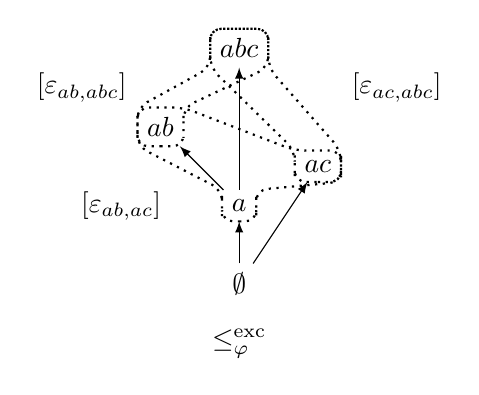
\begin{tikzpicture}
		\node at (0,-0.75){$\le^{\exc}_{\phi}$};
		\node at (0,0)(e){$\emptyset$};
		\node at (0,1)(a){$a$};
		\node at (-1,2)(ab){$ab$};
		\node at (0,3)(abc){$abc$};
		\node at (1,1.5)(ac){$ac$};
		\node at (-2,2.5){$[\px_{ab,abc}]$};
		\node at (2,2.5){$[\px_{ac,abc}]$};
		\node at (-1.5,1){$[\px_{ab,ac}]$};
		\path[-latex] 
		(e) edge (a)
		(a) edge (ab)
		(a) edge (abc)
		(e) edge (ac);
		\draw[thick, dotted, rounded corners=4pt]
			(ab.south)--
			(ab.south east)--
			(ab.east)--
			(ab.north east)--
			(abc.south east)--
			(abc.east)--
			(abc.north east)--
			(abc.north)--
			(abc.north west)--
			(abc.west)--
			(abc.south west)--
			(ab.north west)--
			(ab.west)--
			(ab.south west)--
			(ab.south);
		\draw[thick, dotted, rounded corners=4pt]
			(ac.south)--
			(ac.south east)--
			(ac.east)--
			(ac.north east)--
			(abc.south east)--
			(abc.east)--
			(abc.north east)--
			(abc.north)--
			(abc.north west)--
			(abc.west)--
			(abc.south west)--
			(ac.north west)--
			(ac.west)--
			(ac.south west)--
			(ac.south);
		\draw[thick, dotted, rounded corners=4pt]
			(a.south)--
			(a.south east)--
			(a.east)--
			(a.north east)--
			(ac.south east)--
			(ac.east)--
			(ac.north east)--
			(ac.north)--
			(ac.north west)--
			(ab.north east)--
			(ab.north)--
			(ab.north west)--
			(ab.west)--
			(ab.south west)--
			(a.north west)--
			(a.west)--
			(a.south west)--
			(a.south);
		\end{tikzpicture}
		\caption{
			Exclusive $\re$-revealed preorder $\le^{\exc}_{\phi}$ 
			that is invalidated by postulate $\ppr{\SCON}$,
			even though we would like to see $\le^{\exc}_{\phi}$
			allowed.
		}
		\label{fig:6-hhh-revision-scon-exh-not-good-for-excl}
\end{figure}

\begin{xmpl}{Postulate $\ppr{\SCON}$ does not work for partial preorders}{6-hhh-revision-scon-exh-not-good-for-excl}
	Consider an $\HHH$-revision operator $\re$
	and a Horn formula $\phi$ 
	with $[\phi]=\{\emptyset\}$,
	for which 
	$[\phi\re \px_{ab,abc}]=\{ab,abc\}$,
	$[\phi\re \px_{abc,ac}]=\{abc,ac\}$
	$[\phi\re \px_{ab,ac}]=\{a,ac\}$
	and $\phi\re \px_{\emptyset,w}=\{\emptyset\}$,
	for any interpretation $w$.
	Note that this set of revision results is perfectly consistent 
	with postulates $\ppr{5}$ and $\ppr{7-8}$
	and, furthermore, 
	induces the following exclusive ranking $\le^{\exc}_{\phi}$:
	$ab$, $abc$ and $ac$ are pairwise $\le^{\exc}_{\phi}$-incomparable,
	with the same going for $a$ and $ac$,
	$a<^{\exc}_{\phi}ab$.
	The preorder $\le^{\exc}_{\phi}$ is depicted
	in Figure \ref{fig:6-hhh-revision-scon-exh-not-good-for-excl}.
	This is a legitimate partial preorder, that should be allowed.
	However, under postulate $\ppr{\SCON}$, this setup
	is disallowed.
	Note, we have that: 
	\begin{align*}
		[(\phi\re \px_{ab,abc})\land\px_{ab}]&=\{ab\},\\
		[(\phi\re \px_{abc,ac})\land\px_{abc}]&=\{abc\},\\
		[(\phi\re \px_{ac,ab})\land\px_{ac}]&=\{ac\},\\
		[(\phi\re \px_{ac,ab})\land\px_{ab}]&=\emptyset.
	\end{align*}
	Thus, if we take $w_1 = ab$, $w_2 = abc$ and $w_3 = ac$,
	the setup summarized in Figure \ref{fig:6-hhh-revision-scon-exh-not-good-for-excl}
	would constitute a counter-example to 
	postulate $\ppr{\SCON}$,
	since in this case postulate $\ppr{\SCON}$
	implies that it is not possible to have 
	$(\phi\re \px_{ac,ab})\land\px_{ac}$ consistent
	and 
	$(\phi\re \px_{ac,ab})\land\px_{ab}$ inconsistent.
\end{xmpl}

Example \ref{ex:6-hhh-revision-scon-exh-not-good-for-excl} shows 
that postulate $\ppr{\SCON}$, in conjunction with postulates $\ppr{1-5}$
and $\ppr{7-8}$, leads to unwanted effects, as it eliminates 
preorders that we would like to allow.
Postulate $\ppr{\HSCON}$ is the postulate we need for this case.

That being said, property $\oor{\HSCON}$, which postulate $\ppr{\HSCON}$
guarantees, is still closely connected to Suzumura consistency, which property $\oor{\SCON}$
encodes. In particular, $\oor{\HSCON}$ can be seen as a more specialized version of 
Suzumura consistency, tweaked to work with preorders revealed by $\HHH$-revision operators.
Proposition \ref{prop:6-hhh-revision-HSCON-hscon} shows that, in this context,
property $\oor{\HSCON}$ actually implies Suzumura consistency.

\begin{prp}{}{6-hhh-revision-HSCON-hscon}%
	If $\re$ is an $\HHH$-revision operator that
	satisfies postulates $\ppr{1-5}$ and $\ppr{7-8}$,
	and the exclusive revealed assignment $\as^{\exc}$ satisfies 
	property $\oor{\HSCON}$, then
	$\as^{\exc}$ also satisfies property $\oor{\SCON}$.
\end{prp}
\begin{prf*}{}{}%
	Recall that, in the context of an exclusive revealed assignment $\as^{\exc}$,
	a preference order $\le^{\exc}_{\phi}$ is strict for any distinct interpretations 
	$w_1$ and $w_2$.
	Take, then, pairwise distinct interpretations 
	$w_1$, \dots, $w_n$ such that
	$w_1 <^{\exc}_{\phi}\dots <^{\exc}_{\phi} w_n$
	and suppose,
	in addition, that $w_n <^{\exc}_{\phi} w_1$.
	By the definition of the exclusive revealed 
	assignment, 
	this means that $w_n\in[\phi\re\px_{1,n}]$,
	which, by Lemma \ref{lem:6-hhh-revision-choice-min},
	implies that $w_n\in\min_{\le^{\exc}_{\phi}}\cl_{\horn}(\{w_1,w_n\})$.
	But this contradicts the fact that $\le^{\exc}_{\phi}$
	satisfies property $\oor{\HSCON}$.
\end{prf*}

One of the effects of Proposition \ref{prop:6-hhh-revision-HSCON-hscon}, 
when combined with Theorem \ref{thm:2-suzumura-consistency},
implies that the exclusive revealed preorders 
of an exclusive $\HHH$-revision operator can also be extended
to total preorders on outcomes, as long as the assignment can 
be shown to satisfy property $\oor{\HSCON}$.
For our purposes, though, total preorders are overkill,
since partial preorders are all we are looking for.
Theorem \ref{thm:6-hhh-revision-partial-repr} shows that,
given all the conceptual legwork done so far, 
such partial preorders is within easy reach:
though not exactly the exclusive revealed rankings,
they can be elicited from them by the transitive closure.

\begin{thm}{}{6-hhh-revision-partial-repr}
	An $\HHH$-revision operator $\re$ 
	satisfies postulates $\ppr{1-5}$, $\ppr{7-8}$ (i.e., is exclusive)
	and postulate $\ppr{\HSCON}$
	if and only if there exists
	an $\L_{\horn}$-assignment $\as$ on interpretations
	that 
	satisfies properties $\oor{1-2}$, $\oor{4}$, $\oor{6-7}$ and $\oor{\HC}$
	(i.e., is partial, syntax independent, r-faithful and 
	Horn compliant) 
	and that represents the operator $\re$.
\end{thm}
\begin{prf*}{}{}%
	(``$\Leftarrow$'')
	Take, first, an assignment $\as$ that satisfies the 
	specified conditions.
	Since $\as$ is Horn compliant, this
	implies that the $\as$-induced operator $\re^{\as}$ is an $\HHH$-revision operator.
	Checking that $\re^{\as}$ satisfies postulates $\ppr{1-5}$, $\ppr{7-8}$ is routine.
	Satisfaction of postulate $\ppr{\HSCON}$ 
	follows using Theorem \ref{thm:6-hhh-revision-HSCON-hscon}.

	(``$\Rightarrow$'')
	Take, now, an $\HHH$-revision operator $\re$ that satisfies 
	postulates $\ppr{1-5}$, $\ppr{7-8}$ and $\ppr{\HSCON}$,
	and the $\re$-revealed exclusive $\L_{\horn}$-assignment $\as^{\exc}$.
	If $\phi$ is a Horn formula,
	then the preorder $\le^{\exc}_{\phi}$ is neither complete, nor transitive.
	We know, however, by Theorem \ref{thm:6-hhh-revision-HSCON-hscon},
	that $\le^{\exc}_{\phi}$ satisfies property $\oor{\HSCON}$.

	We take $\le^{\ast}_{\phi}$ to be the transitive 
	and reflexive closure of $\le^{\exc}_{\phi}$,
	and the assignment $\as^{\ast}$ to be defined by $\as^{\ast}\!\!(\phi) \defeq \le^{\ast}_{\phi}$.
	We show, now, that $\as^{\ast}$ is the assignment we are looking for.
	We have that $\as^{\ast}$ is reflexive and transitive by definition,
	and using postulate $\ppr{2}$ it can be shown in the usual way that $\as^{\ast}$ is r-faithful.
	The only thing left to be shown is that $\as^{\ast}$ represents $\re$,
	i.e., that $[\phi\re\mu]=\min_{\le^{\ast}_{\phi}}[\mu]$.
	We show this by double inclusion.

	(``$\subseteq$'')
	Take $w\in[\phi\re\mu]$ and suppose $w\notin\min_{\le^{\ast}_{\phi}}[\mu]$.
	This means that there exists $w'\in[\mu]$ such that $w'<^{\ast}_{\phi}w$,
	i.e., that there exist pairwise distinct interpretations 
	$w_0$, \dots, $w_k$ such that:
	$$
		w'<^{\exc}_{\phi} w_0<^{\exc}_{\phi}\dots <^{\exc}_{\phi}w_k <^{\exc}_{\phi} w.
	$$
	Since $\le^{\exc}_{\phi}$ satisfies property $\oor{\HSCON}$,
	it follows that $w\notin\min_{\le^{\exc}_{\phi}}\cl_{\horn}(\{w_1,w_n\})$.
	At the same time, we have that:
	\begin{align*}
		(\phi\re\mu)\land\px_{w,w'}&\models \phi\re(\mu\land\px_{w,w'}) &\text{by}~\ppr{5}\\
										&\equiv \phi\re\px_{w,w'}. &\text{by}~\ppr{4}
	\end{align*}
	Since $w\in[\phi\re\mu]$, this implies that $w\in[\phi\re\px_{w,w'}]$
	and,
	using Lemma \ref{lem:6-hhh-revision-choice-min}
	we conclude that $w \in\min_{\le^{\exc}_{\phi}}\cl_{\horn}(\{w_1,w_n\})$,
	which creates a contradiction.

	(``$\supseteq$'')
	Take $w\in\min_{\le^{\ast}_{\phi}}[\mu]$ and an arbitrary interpretation 
	$w'\in[\mu]$. We will show first that $w\in[\phi\re\px_{w,w'}]$.
	Suppose that $w\notin[\phi\re\px_{w,w'}]$.
	Since $[\px_{w,w'}]=\cl_{\horn}(\{w,w'\})$,
	there are two relevant cases to look at.

	\emph{Case 1}.
	If $[\phi\re\px_{w,w'}]=\{w'\}$ or $[\phi\re\px_{w,w'}]=\{w',w\cap w'\}$,
	then, by the definition of $\le^{\exc}_{\phi}$
	it follows that $w'<^{\exc}_{\phi}w$,
	which implies that $w'<^{\ast}_{\phi}w$,
	contradicting the fact that $w\in\min_{\le^{\ast}_{\phi}}[\mu]$.

	\emph{Case 2}.
	If $[\phi\re\px_{w,w'}]=\{w\cap w'\}$, then we have that:
	\begin{align*}
		\phi\re\px_{w,w\cap w'} &\models \px_{w,w'},\\
		\phi\re\px_{w,w'} &\models \px_{w,w\cap w'}.
	\end{align*}
	Using postulate $\ppr{7}$, 
	it follows that 
	$\phi\re\px_{w,w\cap w'}\equiv \phi\re\px_{w,w'}$,
	i.e., $[\phi\re\px_{w,w\cap w'}]=\{w\cap w'\}$.
	This, now, implies that $(w\cap w')<^{\exc}_{\phi} w$,
	from which it follows that $(w\cap w')<^{\ast}_{\phi}w$.
	Since $w\in[\mu]$, $w'\in[\mu]$
	and the fact that $\mu$ is a Horn formula and 
	thus $[\mu]$ is closed under intersection, 
	we infer that $(w\cap w')\in[\mu]$ as well.
	But this, together with the previously inferred 
	statement that $(w\cap w')<^{\ast}_{\phi}w$,
	contradicts the fact that $w\in\min_{\le^{\ast}_{\phi}}[\mu]$.
	We conclude, therefore, that $w\in[\phi\re\px_{w,w'}]$.

	For the final step, we use postulate $\ppr{8}$
	and the fact that $\mu=\bigvee_{w'\in[\mu]}\px_{w,w'}$
	to conclude that $w\in[\phi\re(\bigvee_{w'\in[\mu]}\px_{w,w'})]$.
\end{prf*}

Theorem \ref{thm:6-hhh-revision-partial-repr} shows that 
partial preorders can be used to represent exclusive 
$\HHH$-revision operators, just like total preorders can be used to 
represent exhaustive $\HHH$-revision operators.
In doing so, some additions need to be made, both on the semantic side
and on the syntactic side. Firstly, Horn compliance 
works with both total and partial preorders, and guarantees that 
revision always falls within the Horn fragment.
Then, Suzumura consistency, together with its accompanying postulate,
kicks in to make sure that the revealed assignments do not contain cycles
or other unwanted side effects. Interestingly, Suzumura consistency needs 
to be slightly modified in order to work for partial preorders and postulates 
$\ppr{1-5}$ and $\ppr{7-8}$.









\section{Horn update by Horn formulas}\label{sec:6-hhh-update}
All the wisdom gained in Section \ref{sec:6-hhh-revision} can be put to 
use to understand update with Horn formulas,
and this section is dedicated to spelling out the details.
Since the primary plot points for Horn update are the same as for Horn revision with 
Horn formulas, we defer to the previous section for discussion and motivation.

An \emph{$\HHH$-update operator $\up$} is a function  
$\up\colon\L_{\horn}\times\L_{\horn}\rightarrow\L_{\horn}$,
taking as input two Horn formulas, 
typically denoted by $\phi$ and $\mu$
and referred to as the prior and new information, respectively,
and returning a Horn formula,
typically denoted by $\phi\up\mu$
and referred to as the posterior updated information.
The postulates for $\HHH$-update revision
are the standard update postulates $\ppu{1-9}$
as presented in Section \ref{sec:3-update},
and particularized, as for revision, to Horn formulas.
The postulates are expected to 
apply to any Horn formulas
$\phi$, $\phi_{1}$, $\phi_{2}$,
$\mu$, $\mu_{1}$ and $\mu_{2}$
and complete Horn formulas $\dot{\phi}$:

\begin{description}
	\item[($\ppu{1}$)] $\phi\up\mu\models\mu$.	
	\item[($\ppu{2}$)] If $\phi\models\mu$, then $\phi\up\mu\equiv\phi$.
	\item[($\ppu{3}$)] If $\phi$ and $\mu$ are consistent, 
		then $\phi\up\mu$ is consistent.
	\item[($\ppu{4}$)] If $\phi_1\equiv\phi_2$ and $\mu_1\equiv\mu_2$, 
		then $\phi_1\up\mu_1\equiv\phi_2\up\mu_2$.
	\item[($\ppu{5}$)] $(\phi\up\mu_1)\land\mu_2\models\phi\up(\mu_1\land\mu_2)$.
	\item[($\ppu{6}$)] If $(\dot{\phi}\up\mu_1)\land\mu_2$ is consistent, 
		then $\dot{\phi}\up(\mu_1\land\mu_2)\models(\dot{\phi}\up\mu_1)\land\mu_2$.
	\item[($\ppu{7}$)] If $\phi\up\mu_1\models\mu_2$ and $\phi\up\mu_2\models\mu_1$, 
		then $\phi\up\mu_1\equiv\phi\up\mu_2$
	\item[($\ppu{8}$)] If $\mu\equiv \mu_{1}\lor\mu_{2}$.
		then $(\dot{\phi}\up\mu_1)\land(\dot{\phi}\up\mu_2)\models\dot{\phi}\up\mu$.
	\item[($\ppu{9}$)] If $\phi\equiv\phi_1\lor\phi_2$,
		then $(\phi_{1}\lor\phi_{2})\up\mu\equiv(\phi_1\up\mu)\lor(\phi_2\up\mu)$.
\end{description}

As for $\L$-update, we are more interested in the variant of postulate
$\ppu{9}$ presented below.
Since we are working in the Horn fragment, 
this means that proxies are intended to be Horn formulas:
in other words, if $v$ is an interpretations, then 
$\px_{v}$ is an $\L_{\horn}$-proxy of $\{v\}$,
i.e., a Horn formula such that $[\px_{v}]=\cl_{\horn}(\{v\})=\{v\}$.

\begin{description}
	\item[($\ppu{10}$)] $\phi\up\mu\equiv \bigvee_{v\in[\phi]}(\px_{v}\up\mu)$.
\end{description}

Postulate $\ppu{10}$ is equivalent to postulate $\ppu{9}$ 
even when applied to Horn formulas, 
and says that $\phi\up\mu$ can be decomposed
in the results for $\px_{v}\up\mu$, for every $v\in[\phi]$.

On the semantic side we can use, as for $\L$-update, 
assignments on complete formulas: every complete formula is,
or can be thought of, as a Horn formula, 
in the sense that its set of models is $\horn$-closed.
Thus, we can work here with n \emph{$\L_{\comp}$ assignment $\as$ on interpretations}, 
which is a function $\as\colon\L_{\comp}\rightarrow 2^{\U\times\U}$,
taking as input a complete formula $\dot{\phi}$ and returning
a binary relation on interpretations.
The properties we are interested in are as follows, 
for any complete Horn propositional formulas $\dot{\phi}$, $\dot{\phi_{1}}$, $\dot{\phi_{2}}$
and interpretations $w$, $v$, $w_1$ and $w_2$:

\begin{description}
	\item[($\oou{1}$)] $w\le_{\dot{\phi}} w$.
	\item[($\oou{2}$)] If $w_1\le_{\dot{\phi}} w_2$ and $w_2\le_{\dot{\phi}} w_3$, 
		then $w_1\le_{\dot{\phi}} w_3$.
	\item[($\oou{3}$)] $w_1\le_{\dot{\phi}} w_2$ or $w_2\le_{\dot{\phi}} w_1$.
	\item[($\oou{4}$)] If $\dot{\phi_1}\equiv \dot{\phi_2}$, then $\le_{\dot{\phi_1}} = \le_{\dot{\phi_2}}$. 
	\item[($\oou{5}$)] If $[\dot{\phi}]=\{v\}$ and $w\neq v$, then $v<_{\dot{\phi}} w$.
\end{description}

As usual, an $\L_{\comp}$-assignment $\as$ on interpretations is 
\emph{partial} if it satisfies properties $\oou{1-2}$,
\emph{total} if it satisfies properties $\oou{1-3}$,
\emph{syntax insensitive} if it satisfies property $\oou{4}$
and \emph{u-faithful} if it satisfies property $\oou{5}$.

If $\up$ is an $\HHH$-update operator and 
$\as$ is an $\L_{\comp}$-assignment on interpretations,
then \emph{$\as$ represents $\up$}
(and \emph{$\up$ is represented by $\as$})
if, for any Horn formulas $\phi$ and $\mu$,
it holds that $[\phi\up\mu] = \bigcup_{v\in[\phi]}\min_{\le_{\px_{v}}}[\mu]$. 
Given an $\L_{\comp}$-assignment $\as$ on interpretations, 
the \emph{$\as$-induced $\L$-update operator $\re^\as$} is defined,
for any Horn formulas $\phi$ and $\mu$, 
by taking:
$$
	[\phi\up^\as\mu]\defeq\bigcup_{v\in[\phi]}\min_{\le_{\px_{v}}}[\mu].
$$
If $\up$ is an $\HHH$-update operator and $\dot{\phi}$ is a complete (Horn) formula,
the \emph{exhaustive $\up$-revealed plausibility relation $\le^\exh_{\dot{\phi}}$} 
and the \emph{exclusive $\up$-revealed plausibility relation $\le^\exc_{\dot{\phi}}$} 
are defined, for any interpretations $w_1$ and $w_2$, respectively, as:
\begin{align*}
	w_1\le^\exh_{\dot{\phi}} w_2 &~\text{if}~w_1\in[{\dot{\phi}}\up\px_{1,2}],\\
	w_1\le^\exc_{\dot{\phi}} w_2 &~\text{if either}~w_1=w_2,
			\text{or}~w_1\in[{\dot{\phi}}\up\px_{1,2}]~\text{and}~w_2\notin[{\dot{\phi}}\up\px_{1,2}].
\end{align*}
The \emph{exhaustive $\up$-revealed $\L_{\comp}$-assignment $\as^\exh$} 
and \emph{exclusive $\up$-revealed $\L_{\comp}$-assignment $\as^\exc$} 
are obtained by taking $\as^\exh\!\!(\dot{\phi})=\le^\exh_{\dot{\phi}}$ 
and $\as^\exc\!\!(\dot{\phi})=\le^\exc_{\dot{\phi}}$, for any complete 
Horn formula $\dot{\phi}$.
As for revision,
$\up^{\as}$ is defined as an $\L$-update operator,
i.e., an operator that returns propositional formulas and
not necessarily Horn formula,
because an assignment needs to be restricted if it is to deliver 
results compatible with the Horn fragment.

Since update becomes indistinguishable from revision when $\phi$
is complete, the same problems that plague $\HHH$-revision also occur 
when working with $\HHH$-update operators.
Note, for instance, that the prior information in 
Examples \ref{ex:6-hhh-revision-standard-ops-no-good} is complete:
this shows that this example is relevant to $\HHH$-update as well 
and, in particular, that existing update operators, such as Forbus and Winslett's
operators do not work as $\HHH$-update operators.
The solution, of course, is to restrict the assignments we are working with 
using a property that, 
as we might expect, is a version of Horn compliance adapted to the context 
of update.
This property says that the following must hold,
for any Horn formulas $\phi$ and $\mu$:

\begin{description}
	\item[($\oou{\HC}$)] $\bigcup_{v\in[\phi]}\min_{\le_{\px_{v}}}[\mu]$ is $\horn$-closed.
\end{description}


% This property applies for any interpretations $w_1$, $w_2$
% and complete Horn formulas $\dot{\phi_{1}}$ and $\dot{\phi_{2}}$:

% \begin{description}
% 	\item[($\oou{\dTCMPL}$)] If $w_1 \not<_{\dot{\phi}}w_2$ and $w_2\not<_{\dot{\phi}}w_1$, 
% 		then there exists a complete formula $\dot{\phi_{3}}$ such that		
% 		$(w_1\cap w_2) \in\min_{\le_{\dot{\phi_{3}}}}\cl_{\horn}(\{w_1,w_2\})$.
% \end{description}

Property $\oou{\HC}$, 
where `$\HC$' stands for \emph{Horn compliance},
works along the same lines as Horn compliance 
in the context of $\HHH$-revision \cite{DelgrandeP15},
and ensures that the $\as$-induced update operator 
is an $\HHH$-update operator.



% As with property $\oor{\TCMPL}$, the goal of property $\oou{\dTCMPL}$
% is to ensure that a $\L_{\comp}$-assignment on interpretations
% can represent an $\HHH$-update operator.

% \begin{thm}{}{6-hhh-update-dTCMPL-well-defined}
% 	If $\up$ is an $\L$-update operator
% 	and $\as$ is an $\L_{\comp}$-assignment on interpretations
% 	that represents it,
% 	then $\up$ is an $\HHH$-update operator, 
% 	when restricted to Horn formulas,
% 	if and only if $\up$ satisfies property $\oou{\dTCMPL}$,
% 	when restricted to Horn formulas.
% \end{thm}
% \begin{prf*}{}{}%
	
% \end{prf*}

Furthermore, Examples \ref{ex:6-hhh-revision-cycles} and \ref{ex:6-hhh-revision-scon-exh-not-good-for-excl}
can also be adapted to $\HHH$-update operator, 
showing that the standard postulates do not exclude unwanted assignments.
The fixes, as for $\HHH$-revision, involve 
a series of semantic properties on the revealed preference orders,
coupled with corresponding logical postulates.
The semantic properties are intended to apply for any 
complete Horn formulas $\dot{\phi}$
and interpretations $w_1$, \dots, $w_n$, and are as follows:

\begin{description}
	\item[($\oou{\SCON}$)] If $w_1 \le_{\dot{\phi}}\dots \le_{\dot{\phi}}w_n$,
	then $w_{n}\not<_{\dot{\phi}} w_{1}$.
	\item[($\oou{\HSCON}$)] If $w_1 <_{\dot{\phi}}\dots <_{\dot{\phi}} w_n$,
	then $w_n\notin\min_{\le_{\dot{\phi}}}\cl_{\horn}(\{w_1,w_n\})$.
\end{description}

These properties are equivalent to properties $\oor{\SCON}$ and $\oor{\HSCON}$,
with the only difference being that they are particularized to complete Horn formulas.
As expected, property $\oou{\SCON}$ is expected to hold for the exhaustive 
revealed assignment and $\oou{\HSCON}$ is intended to hold for the exclusive 
revealed assignment.

On the syntactic side 
we use the following postulates,
or more precesily postulate schemas,
intended to work for any complete Horn formulas $\dot{\phi}$,
interpretations $w_1$, \dots, $w_n$
and the corresponding $\L_{\horn}$-proxies:

\begin{description}
	\item[($\ppu{\SCON}$)]
	If $(\dot{\phi}\up\px_{1,2})\land\px_{1}$ is consistent,
		\dots,
		$(\dot{\phi}\up\px_{n-1,n})\land\px_{n-1}$ is consistent,
	then it does not hold both that
	$(\dot{\phi}\up\px_{n,1})\land\px_{n}$ is consistent
	and that $(\dot{\phi}\up\px_{n,1})\land\px_{1}$ is inconsistent.

	\item[($\ppu{\HSCON}$)]
	If 
		$(\dot{\phi}\up\px_{1,2})\land\px_{1}$ is consistent and
		$(\dot{\phi}\up\px_{1,2})\land\px_{2}$ is inconsistent,
		\dots,
		$(\dot{\phi}\up\px_{n-1,n})\land\px_{n-1}$ is consistent and
		$(\dot{\phi}\up\px_{n-1,n})\land\px_{n}$ is inconsistent,
	then $(\dot{\phi}\up\px_{n,1})\land\px_{n}$ is inconsistent.
\end{description}

Postulates $\ppu{\SCON}$ and $\ppu{\HSCON}$ are direct rewritings of postulates 
$\ppr{\SCON}$ and $\ppr{\HSCON}$ from $\HHH$-revision,
and the argument that they go hand in hand with propeerties $\oou{\SCON}$ and $\oou{\HSCON}$
is entirely similar.

With most of the theoretical groundwork having been laid in Section \ref{sec:6-hhh-revision},
the representation results can be stated now in quick succession.
The first result concerns $\HHH$-update operators that satisfy postulates $\ppu{1-6}$, $\ppu{9}$
and $\ppu{\SCON}$, and are represented using total assignments.

\begin{thm}{}{6-hhh-update-repr-total}
	An $\HHH$-update operator $\up$ 
	satisfies postulates $\ppu{1-6}$, $\ppu{9}$ and $\ppu{\SCON}$
	if and only if there exists
	an $\L_{\comp}$-assignment $\as$ on interpretations
	that satisfies properties $\oou{1-5}$ and $\oou{\HC}$
	(i.e., is total, syntax independent, u-faithful and Horn compliant)
	and that represents the operator $\up$.
\end{thm}
\begin{prf*}{}{}%
	Horn compliance of $\as$ guarantees that the $\as$-induced update operator $\up^{\as}$ 
	is an $\HHH$-update operator, and showing that $\up^{\as}$ satisfies postulates 
	$\ppu{1-6}$, $\ppu{9}$ and $\ppu{\SCON}$ is straightforward, and works in the same way 
	as for $\HHH$-revision operators.
	Conversely, if $\up$ satisfies postulates $\ppu{1-6}$, $\ppu{9}$ and $\ppu{\SCON}$,
	then we use the argument for $\HHH$-revision operators that satisfy postulates $\ppr{1-6}$,
	particularized to complete formulas.
	That is to say, using Theorem \ref{thm:6-hhh-revision-total-repr},
	we know that the $\up$-revealed exhaustive assignment represents $\up$ for the case of complete formulas,
	i.e., if $\dot{\phi}$ is a complete Horn formula,
	then $[\dot{\phi}\up\mu]=\min_{\le_{\dot{\phi}}}[\mu]$, for any Horn formula $\mu$.
	We now use postulate $\ppu{9}$ to extend this to the fact that 
	$[\phi\up\mu]=\bigcup_{v\in[\phi]}\min_{\le_{\px_{v}}}[\mu]$,
	for any Horn formula $\phi$.
	This shows that $\as^{\exh}$ represents the operator $\up$.
\end{prf*}

Accompanying this result is, of course, a result for 
$\HHH$-update operators that satisfy postulates $\ppu{1-5}$, $\ppu{7-8}$, $\ppu{9}$
and $\ppu{\HSCON}$, and are represented using partial assignments.

\begin{thm}{}{6-hhh-update-repr-partial}
	An $\HHH$-update operator $\up$ 
	satisfies postulates $\ppu{1-5}$, $\ppu{7-8}$, $\ppu{9}$ and $\ppu{\HSCON}$
	if and only if there exists
	an $\L_{\comp}$-assignment $\as$ on interpretations
	that satisfies properties $\oou{1-2}$, $\oou{4-5}$ and $\oou{\HC}$
	(i.e., is partial, syntax independent, u-faithful and Horn compliant)
	and that represents the operator $\up$.
\end{thm}
\begin{prf*}{}{}%
	The proof here follows the same lines as the proof for Theorem \ref{thm:6-hhh-update-repr-total},
	but using the results in Theorem \ref{thm:6-hhh-revision-partial-repr} to construct the 
	revealed assignment that ends up representing the operator $\up$.
\end{prf*}

Theorems \ref{thm:6-hhh-update-repr-total} and \ref{thm:6-hhh-update-repr-partial}
are straightforward applications of Theorems \ref{thm:6-hhh-revision-total-repr} 
and \ref{thm:6-hhh-revision-partial-repr}, but the insights gained in making these results 
work show that they are robust enough to function across different contexts.


























\section{Related work}\label{sec:6-rw}
Work on belief change for the Horn fragment began with 
work on contraction \cite{Delgrande08,DelgrandeW10,DelgrandeW13}, 
the conclusions of which, however, were that traditional AGM techniques,
such as ones based on remainder sets, did not work as expected
in the Horn fragment. Alternative constructions were proposed,
e.g., in terms of \emph{weak remainder sets}, which were later taken 
up and extended \cite{BoothMV09,BoothMVW11,ZhuangP14}.

Getting Horn contraction right is important for revision as well,
since contraction and revision are traditionally thought to be inter-definable
via the Levi and Harper identities \cite{Levi91,Harper76}.
However, these identities involve negations and, since the negation of a Horn formula
is not necessarily a Horn formula, their application to the Horn fragment is limited
\cite{Delgrande08,ZhuangPZ13,ZhuangPZ17}.

Thus, it seems that Horn revision is best thought of on its own.
In this, some of the most promising approaches to revision of Horn formulas 
have been model based: given our understanding of revision 
as a choice function on outcomes, this line of research is particularly apposite.
Indeed, our starting point has been the model developed originally 
by James Delgrande and Pavlos Peppas \cite{DelgrandeP15,DelgrandePW18},
which we have sought to emulate here using 
partial preorders and weaker versions of the classical postulates.
Our understanding of this model and its variations is thoroughly semantic, with the main 
actors, and guarantors of rationality, being the preorders on interpretations:
in our view, as long as we are able to get the right kinds of preorders 
(i.e., transitive, or at least non-cyclic), then we are on the right track.
In this light, the role of the additional postulates is to make sure 
that the preorders behave well: it is difficult to justify a postulate 
such as $\ppr{\SCON}$ or $\ppr{\HSCON}$ other than by appeal to the 
semantic property it induces. This is also why we choose to 
formulate these postulates using $\L_{\horn}$-proxies 
(i.e., as choices over pairs of interpretations)
rather than by using generic Horn formulas, as in \cite{DelgrandeP15,DelgrandePW18}.

This preorder-led view is also what led us to the rational choice literature,
where the relationship between choice functions and various types of preference 
relations has been a mainstay since the very early days. 
Suzumura consistency \cite{Suzumura76,Suzumura83,BossertS10} 
jumped out as the most obvious connecting element, but the rational choice literature 
is awash in distinctions and properties that could be useful to belief change as well. 
For instance, the acyclicity postulate presented in \cite{DelgrandeP15,DelgrandePW18}
occurs in an equivalent formulation in rational choice theory, as the 
\emph{Strong Axiom of Revealed Preference (SARP)} \cite{Hansson68,Suzumura16}.

Belief change in the Horn fragment, as we have seen, is caught in between 
two equally demanding requirements: one is the normative demands 
provided by the postulates,
i.e., the requirement that the revision operator should satisfy a set 
of desirable properties;
the other is the expressibility requirement,
i.e., we need to make sure that the result 
can be expressed as a Horn formula. 
In this chapter we have typically opted to hold fast to the postulates, and even 
complement them if needed, but this has had the effect of limiting the range 
of available operators: none of the tried and tested revision or update operators 
works in the Horn fragment. 
A different approach is to take the existing operators and repair their output when 
it does not fit into the Horn fragment, e.g., by taking the $\horn$-closure of 
the selected set of interpretations as the result. 
The advantage of this method is that it is guaranteed to produce $\horn$-closed
results; the disadvantage is that some of the postulates might not be satisfied 
\cite{CreignouPPW14,CreignouPRW16,CreignouKP18}.

It should also be mentioned that belief change in fragments is not 
confined to contraction and revision (or update), 
with existing work on merging in the Horn fragment
\cite{HaretRW15,HaretRW17},
and the Horn fragment is not the 
only formalism of interest,
with logic programs, Answer Set Programs and Description Logics 
all enjoying their own fifteen minutes of AGM fame
\cite{DelgrandeW13,ZhuangWWQ16,BinnewiesZWS18,ZhuangWWD19,ZheleznyakovKNC20}.










\section{Conclusion}\label{sec:6-conclusion}
In this chapter we have looked at revision of Horn formulas 
using both propositional and Horn formulas:
though the results have ultimately taken a familiar form
(i.e., as representation theorems),
the overall work surrounding them shows that restricting the 
language in which belief change occurs does not allow us 
to seamlessly derive the same conclusions.

Over and over, we have seen that the standard postulates 
do not generalize immediately to the Horn fragment.
For revision with propositional formulas, 
the standard postulate $\ppr{2}$ becomes problematic and 
the newly introduced neutrality postulate $\ppr{\NEUT}$
proves impossible to satisfy.
For revision, as well as update, with Horn formulas,
it is postulates $\ppr{5-6}$, and, respectively, $\ppu{5-6}$,
that end up being less powerful at forcing the assignments 
into the right shape.
The solution, we have seen, has been to complement the standard 
postulates by new ones: typically, a special postulate depending 
on whether we were working with total or partial preorders.
In doing so, we extended existing work on revision in the Horn fragment 
\cite{DelgrandeP15,DelgrandePW18},
and revealed some interesting principles that underlie belief change in fragments.

Lemma \ref{lem:6-hhh-revision-choice-min}, in particular, 
is interesting enough that it deserves more consideration:
in essence, it says that if a chain of comparisons 
favors an interpretation $w_1$ over $w_n$, then $w_n$ should not 
be chosen over $w_1$  when the choice 
is over the proxy of $w_1$ and $w_n$.
This property holds for all the settings we have encountered so far 
(total and partial orders, propositional logic as well as its Horn fragment),
but it was only for the Horn fragment with partial preorders that we had 
to spell it out explicitly.
As such, Lemma \ref{lem:6-hhh-revision-choice-min} captures a property that
is likely to prove important for belief change in formalisms other than
propositional logic and the Horn fragment.








\chapter{Preference Change}\label{ch:7}

Preferences play a central role in theories of decision making
as part of the mechanism underlying intentional behavior and rational choice:
they show up in economic models of rational 
agency \cite{MasColell95,Sen17},
as well as in formal models of artificial agents 
supposed to interact with the world and each 
other \cite{BoutilierBDHP04,DomshlakHKP11,RossiVW11,PigozziTV16}.
Since such interactions take place in dynamic environments, 
it can be expected that preferences change in response to new developments.

In this chapter we are interested in preference change 
occurring when new preference information,
denoted by $\o$, becomes available and has to be taken at face value, 
thereby prompting a change in prior preference information, denoted by $\p$.
The change, we require, should preserve as much useful information from $\p$
as can be afforded.

We believe that preference change thus described is a pervasive phenomenon, 
arising in many contexts straddling the realms of both human and artificial agency.
Thus, there is a distinguished tradition in economics and philosophy
puzzling over examples of conflict between an agent's subjective preference
(what we call here the initial, or prior preference $\p$) 
and a second-order preference,
often standing for a commitment or moral rule 
(what we call here the new preference information $\o$):
the need to reconcile such a conflict is widely acknowledged, but in the absence
of a concrete mechanism for doing so its presence is more often than not 
simply signaled as a problem that besets real life agents.
% \cite{Harsanyi55,Jeffrey74,Sen77,Frankfurt88,Nozick94}.

One example of the phenomenon that leads to preference revision
occurs in the philosopher Harry Frankfurt's discussion on  
\emph{second-order volitions}, which are desires about desires.
According to Frankfurt, an agent's second-order volition with respect 
to a desire $D$ is a desire that $D$ be the agent's will, 
i.e., that $D$ determines the agent's actions:
\begin{quote}
	Besides wanting and choosing and being moved to do this or that, 
	[people] may also want to have (or not to have) certain desires and motives. 
	They are capable of wanting to be different, 
	in their preferences and purposes, from what they are.
	\cite{Frankfurt88}
\end{quote}

The existence of second-order volitions is taken by Frankfurt 
to be a hallmark of personhood:

\begin{quote}
	\dots it is having second-order volitions [\dots] 
	that I regard as essential to being a person.
	\cite{Frankfurt88}
\end{quote}

Frankfurt does not mention preferences explicitly but, 
since in standard models of rational agency
preferences are taken to be part of what determines action, 
we can imagine that his point applies to preferences as well as desires.
Preferences do appear in subsequent discussions, for instance
in Robert Nozick's account of the same phenomenon:

\begin{quote}
	A person lacks rational integration when [they] prefer some alternative $x$ 
	to another alternative $y$, yet [they] prefer that [they] 
	did not have this preference, 
	that is, when [they] also prefer not preferring $x$ to $y$ 
	to preferring $x$ to $y$. 
	When such a second-order preference conflicts with a first-order one, 
	it is an open question which of these preferences should be changed. 
	What is clear is that they do not hang together well, 
	and a rational person would prefer that this not (continue to) be the case.
	\cite{Nozick94}
\end{quote}

Nozick's formulation brings us closer to the framework 
we will be using in this chapter, of preference orders battling it out.
If we assimilate his second order preferences to Frankfurt's second 
order volitions, then we have the same problem of a mismatch, 
or `lack of integration',
between the agent's preferences.
Nozick confines himself to just labeling the problem and does not tell 
us how to solve it, but we are led to understand that it is,
notwithstanding, a problem.
The same issue arises in economist John C. Harsanyi's
distinction between an individual's 
\emph{social welfare function} and their \emph{personal utility function},
two notions that refer to two distinct types of preferences:

\begin{quote}
	\dots the former [type of preference] 
	must express what this individual prefers 
	(or rather, would prefer) on the basis of 
	impersonal social considerations alone, 
	and the latter must express what he actually prefers, 
	whether on the basis of his personal 
	interests or on any other basis. 
	The former may be called his `ethical' preferences, 
	the latter his `subjective' preferences.
	\cite{Harsanyi55}
\end{quote}

In Harsanyi's phrasing, the problem is, as for Nozick, one of conflict
between preferences: humans are the kind of beings that can 
entertain two types of preferences at the same time,
and sometimes these preferences are not perfectly aligned.
At the same time, Harsanyi seems to suggest, the ethical preferences
(which we may assimilate with Frankfurt's second order desires
and Nozick's second order preferences)
enjoy a certain type of prestige over the other,
such that in a perfect world the subjective preferences 
would coincide with the ethical preferences,
but in the imperfect world we live in the two are sometimes 
at odds with one another.
That this is eminently possible is, of course, 
an old adage, and the phenomenon is sometimes called \emph{akrasia}
from the Greek term for lack of will.
A classical example of akrasia occurs with habits that people
want to get rid of, such as smoking: 
an agent smokes, which according to the revealed preference paradigm
we have been espousing in the previous chapters,
can be taken to indicate a preference of smoking over non-smoking;
but at the same time, the agent might want to quit,
i.e., to have the opposite preference.
In the context of decision theory, this problem shows up in the form 
of Richard C. Jeffrey's Akrates, 
who would rather be abstinent than smoke:

\begin{quote}
	\dots although Akrates cannot simply choose to prefer abstinence 
	on this occasion---and that, after all, is why his preference 
	for preferring abstinence is (uneasily) compatible with his 
	preference for smoking---he can undertake a project of modifying 
	his preferences over time, so that one day he may regularly prefer 
	abstinence, just as now he regularly prefers smoking. 
	The steps toward this desired end may involve hypnosis, 
	reading medical textbooks, discussing matters with like-minded friends, 
	or whatever. But in accounting for Akrates's undertaking of these 
	activities it seems natural to cite his preference for preferring 
	abstinence, just as in accounting for his activities as he flings 
	drawers open and searches through pockets of suits, 
	one may cite his preference for smoking\dots 
	\cite{Jeffrey74}
\end{quote}

Jeffrey, just like Frankfurt, Nozick and Harsanyi,
is interested here only in pointing out the basic fact 
that Akrates can prefer smoking to abstinence, 
while wishing he had the opposite preference.
Jeffrey assumes that Akrates' problem will be solved 
if Akrates can only get himself, by whatever means necessary,
to change his disposition such that he comes to 
prefers abstinence to smoking.
The challenge Akrates is facing is that he needs to
make sure that his priorities 
are aligned with the preferences specific to a respected source.
The same challenge can occur in technological applications, 
from updating CP-nets~\cite{CadilhacALB15}
to changing the order in which search results 
are displayed on a page in response to user provided specifications.
Similar topics are emerging in the discussion 
on ethical decision making for artificial agents \cite{RossiM19}.
Thus, far from being an issue of narrow interest, 
the problem of changing preferences and 
resolving conflicts along the way is an important 
component of rational agency.

Whether it is the internal conflict between 
an agent's private leanings and the better angels of its nature,
or a content provider wanting to tailor its products 
for a better user experience, 
many cases of preference change involve a conflict
between two types of preferences, one of which is 
perceived as having priority over the other:
we will call this type of change 
\emph{preference revision}, due to its similarity 
with revision as presented in Section \ref{sec:3-revision}.

Up to this point we have been arguing that 
cases of preference revision can arise in several contexts, 
but have not seen any actual mechanism for handling them.
What is Akrates to do?
Indeed, if there are only two alternatives 
to work with,
e.g., smoking and abstinence, 
then it is difficult to see what more can be said,
at the formal level, other than that smoking and abstinence 
should be swapped in Akrates' preference order.
To see that there is more at stake here, 
we must look at an example with more than two alternatives.

\begin{figure}\centering
	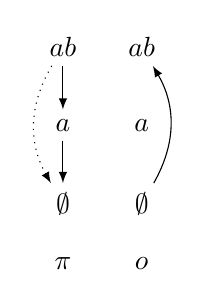
\begin{tikzpicture}
	\node at (0,-0.75){$\p$};
	\node at (0,2)(1){$ab$};
	\node at (0,1)(2){$a$};
	\node at (0,0)(3){$\emptyset$};
	\path[-latex](1)edge(2)(2)edge(3)(1)edge[bend right,dotted](3);
	
	\node at (1,-0.75){$\o$};
	\node at (1,2)(1){$ab$};
	\node at (1,1)(2){$a$};
	\node at (1,0)(3){$\emptyset$};
	\path[-latex](3)edge[bend right](1);
	
	\end{tikzpicture}		
	\caption{
		Preference order $\p$ has to be revised by
		preference $\o$.
		A direct comparison ranking $i$ better than $j$ is
		depicted by a solid arrow from $i$ to $j$, 
		with comparisons inferred by transitivity depicted by dotted arrows.
		To distinguish these types of preference orders 
		from the preference orders used to model belief change operators 
		in assignments, we draw the better elements on top here.
		}
	\label{fig:7-pref-change-3-alternatives}
\end{figure}

\begin{xmpl}{}{7-pref-change-3-alternatives}
	Consider the scenario from Example \ref{ex:1-pref-change-motivation},
	where a doctor is considering treatments for a novel disease. The 
	doctor has two drugs, $a$ and $b$, that can be prescribed alone 
	or in combination with each other. For the purposes of this illustration,
	let us assume the doctor is considering three alternatives:
	either to administer $a$ and $b$ together, denoted by the interpretation $ab$,
	or $a$ alone, denoted by the interpretation $a$,
	or nothing, denoted by $\emptyset$.

	The doctor's initial assessment is that 
	$a$ and $b$ together work better than $a$ alone, which 
	by itself is better than doing nothing.
	This ranking constitutes a preference order, 
	and by virtue of transitivity we can conclude 
	that $a$ and $b$ together are better
	than administering nothing.
	We can write the doctor's preferences as the set 
	$\p=\{(ab,a),(a,\emptyset),(ab,\emptyset)\}$
	of comparisons the doctor bases its assessment on.
	The comparison $(ab,a)$, for instance, is to be read 
	that $ab$ is strictly better than $a$.
	Of the comparisons in $\p$, we may assume that $(ab,a)$ and $(a,\emptyset)$
	are established by the doctor directly,
	while $(ab,\emptyset)$ is inferred by transitivity from the other two.
	The preference order $\p$ is depicted in Figure \ref{fig:7-pref-change-3-alternatives}.

	Afer a while, the doctor becomes convinced that $\emptyset$ is better than $ab$,
	and hence has to modify its initial assessment $\p$ accordingly.
	We can represent the new information as a preference order $\o$ in its own right.
	The preference order $\o$ consists of the comparison $(\emptyset,ab)$,
	i.e., $\o=\{(\emptyset, ab)\}$, 
	and is likewise depicted in Figure \ref{fig:7-pref-change-3-alternatives}.
	Note that simply adding $\o$ to $\p$
	leads to a cycle between the three alternatives,
	i.e., the transitive closure of $\p\cup\o$ implies that 
	$ab$ is strictly better than itself.
	Since the doctor is committed to accepting $\o$,
	then they will have to give up something from $\p$ in order to maintain 
	consistency. 	
\end{xmpl}

Example \ref{fig:7-pref-change-3-alternatives} is not a case of akrasia,
but illustrates the problem just as well:
if new preference information contradicts an existing preference,
in the sense that it leads to a preference cycle,
then some of the comparisons involved in the cycle have to be given up.
The challenge for Akrates, then, is that even after fitting 
the second order preference into his schedule,
he still needs to figure out what the rest of his preference order
looks like. In other words, Akrates has a decision problem on his hands:
since there is no unique way, on logical grounds alone, 
of breaking a preference cycle, some extra information needs to be brought in.
What should this extra information concern?

Based on our experience so far, 
we should expect the answer to be preferences:
indeed, preferences on preferences themselves.
This strategy, which we will be pursuing in the 
rest of this chapter,
has already been anticipated by Amartya Sen:

\begin{quote}
	...we need to consider rankings of preference rankings to express our moral judgments.
	\cite{Sen77}
\end{quote}

We want to pick up Sen's suggestion and 
suggest that preferences over the basic building
blocks of a preference order, 
i.e., the comparisons it is made of, 
offer a way of understanding preference revision.

\begin{figure}\centering
	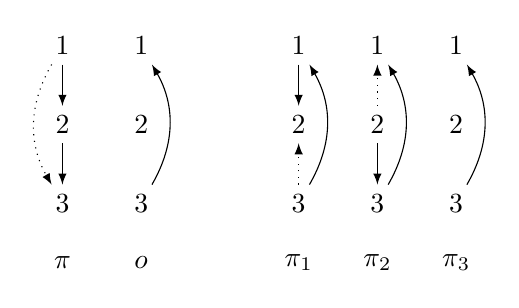
\begin{tikzpicture}
	\node at (0,-0.75){$\p$};
	\node at (0,2)(1){$1$};
	\node at (0,1)(2){$2$};
	\node at (0,0)(3){$3$};
	\path[-latex](1)edge(2)(2)edge(3)(1)edge[bend right,dotted](3);
	
	\node at (1,-0.75){$\o$};
	\node at (1,2)(1){$1$};
	\node at (1,1)(2){$2$};
	\node at (1,0)(3){$3$};
	\path[-latex](3)edge[bend right](1);
	
	\node at (3,-0.75){$\p_1$};
	\node at (3,2)(1){$1$};
	\node at (3,1)(2){$2$};
	\node at (3,0)(3){$3$};
	\path[-latex](3)edge[bend right](1)(1)edge(2)(3)edge[dotted](2);
	
	\node at (4,-0.75){$\p_2$};
	\node at (4,2)(1){$1$};
	\node at (4,1)(2){$2$};
	\node at (4,0)(3){$3$};
	\path[-latex](3)edge[bend right](1)(2)edge(3)(2)edge[dotted](1);
	
	\node at (5,-0.75){$\p_3$};
	\node at (5,2)(1){$1$};
	\node at (5,1)(2){$2$};
	\node at (5,0)(3){$3$};
	\path[-latex](3)edge[bend right](1);
	\end{tikzpicture}		
	\caption{
		Revising preference order $\p$ by $\o$: 
		simply adding $\o$ to $\p$ leads to a cycle,
		so if $\o$ is accepted then a choice needs 
		to be made regarding which of the initial comparisons of $\p$ to keep;
		potential candidates for the revised order are $\p_1$, $\p_2$ or $\p_3$.
		A direct comparison ranking $i$ better than $j$ is	depicted by a solid arrow from $i$ to $j$, 
		with comparisons inferred by transitivity depicted by dotted arrows.
		}
	\label{fig:7-pref-change-3-alternatives-ctd}
\end{figure}

\begin{xmpl}{}{7-pref-change-3-alternatives-ctd}
	We revisit the scenarion in Example \ref{ex:7-pref-change-3-alternatives},
	with a doctor revising their preferences over three treatment options:
	$ab$, $a$ and $\emptyset$.
	To further simplify the problem, we denote the alternatives by 
	integers, such that $1$ stands for $ab$, $2$ stands for $a$ and $3$ stands for $\emptyset$. 
	The initial preference $\p$ is such that,
	as a result of direct comparison, 
	alternative $1$ is ranked better than $2$ 
	and $2$ is ranked better than $3$;
	by virtue of transitivity, it is also inferred that 
	$1$ is considered better than $3$.
	We want to revise $\p$ by a preference $\o$, 
	according to which $3$ is better than $1$. 
	Both preference orders $\p$ and $\o$ are depicted in 
	Figure \ref{fig:7-pref-change-3-alternatives-ctd}.
	%	this means that $\p$ has to be modified to incorporate the comparisons contained in $\o$,
	%	but without giving up more information than strictly necessary.

	The simplest solution is to add $\o$ to $\p$ 
	(i.e., include the comparisons contained in both),
	but the transitivity requirement leads to a cycle between $1$, $2$ and $3$, 
	%	and thus the result fails to be a preference order.
	which we would like to avoid.
	We are thus in a situation where $\p$ and $\o$ cannot be jointly accepted,
	but since $\o$, we stipulate, must be accepted,
	something must be given up from $\p$ (though,
	we ask, no more than strictly necessary). How is the decision to be made?
	We suggest that an implicit preference over the comparisons of 
	$\p$ that were explicitly provided
	can provide an answer: if the comparison of $1$-vs-$2$ 
	(the edge from $1$ to $2$ in Figure \ref{fig:7-pref-change-3-alternatives-ctd})
	is preferred to the one of $2$-vs-$3$ then the result is $\p_1$, which
	holds on to $1$-vs-$2$ from $\p$ and together with $\o$ infers, by transitivity, 
	that $3$ is better than $2$;
	alternatively, a preference for $2$-vs-$3$ over $1$-vs-$2$
	leads to $\p_2$ as the result, while indifference between the two comparisons
	means that both are given up, resulting in $\p_3$.
	Thus, preference over comparisons in $\p$ translates as choice over how to go about revising $\p$.
	Interestingly, we may also reason in the opposite direction:
	observing choice behavior across different instances of revision allows us to infer preferences 
	over comparisons in $\p$, e.g., revising to $\p_1$, rather than to $\p_2$ or $\p_3$,
	can be rationalized as saying that the comparison of $1$-vs-$2$
	is considered better than $2$-vs-$3$.
\end{xmpl}

Our aim in this chapter is to formalize the type of 
reasoning illustrated in Example \ref{ex:7-pref-change-3-alternatives-ctd}
by rationalizing preference change as a type of choice function 
on what we will call the \emph{direct comparisons of $\p$},
i.e., the explicit preferences assumed to be given in $\p$.
Since a conflict between $\p$ and $\o$ forces some of the direct comparisons of $\p$
to be renounced, additional information in the form of a preference order over the direct comparisons
of $\p$ will serve as guide to the choice function.
%Revising an initial preference $\p$ by new preference information $\o$,
%especially if $\p$ and $\o$ are conflicting,
%opens up a range of options, as Example \ref{ex:preferences-3-items} illustrates.
Our purpose, in this, is not to legislate on what is the right choice to make;
rather, it is to make sure that whatever the choice is, it is made in a coherent way.
To this end, we present a set of rationality postulates 
to capture conditions under which the preference order on direct comparisons of $\p$ 
exists and has desired properties.
Thus, the significance of our approach lies in laying bare the theoretical requirements
and basic assumptions for mechanisms intended to revise preferences.

The postulates we put forward bear a distinct resemblance to the AGM postulates 
employed for belief revision
\cite{AlchourronGM85,KatsunoM92,Hansson17,FermeH18}:
given that changing one's mind involves choosing some parts 
of a belief to keep and some to remove,
this is no coincidence. 
Indeed, the two problems are similar, 
though the structural particularities of preferences
(in particular, the requirement that they are transitive) 
mean that transfer of insights from belief revision 
to preference revision is by no means straightforward.

%In this paper, we model preference change arising out of an interaction between two elements:
%the first is an initial preference ranking, typically denoted by $\p$,
%which encodes a pre-existing attitude;
%the second element is new preference information $\o$ signaling input from an authoritative source,
%which may come into conflict with the information in $\p$.
%The assumption is that $\o$ has priority,
%but that $\p$ contains useful information which should not be discarded unless absolutely necessary.
%Thus, the presence of $\o$ triggers a change in $\p$, 
%the latter having to be modified in an efficient way such that it accommodates $\o$:
%the end goal is to bring $\p$ in line with $\o$, without having to give up more of $\p$ than is needed.
%Formally, this is performed by a change operator $\en$,
%the result of which is a new preference order, typically denoted by $\p\en\o$,
%which fully incorporates $\o$ while preserving as much as possible from the pre-existing order $\p$. 


% The rest of the paper contains our contributions, summarized as follows. 
% In Section \ref{sec:preliminaries}
% we introduce basic notation.
% In Section \ref{sec:semantics} we provide a constructive way of revising a preference order,
% based on rankings of the direct comparisons.
% In Section \ref{sec:postulates} we provide a set of intuitive postulates 
% and we show that they characterize the procedure described in Section \ref{sec:semantics}.
% Section \ref{sec:concrete-operator} discusses concrete preference revision operators,
% and Section \ref{sec:conclusion} offers concluding remarks.














\section{Strict partial orders}\label{sec:7-spos}
We assume a finite set $V$ of items, 
standing for the objects an agent can have preferences over.
In keeping with the pattern established so far, 
a preference order is construed as a transitive binary relation on $V$, 
though in a break with standard practice 
the preferences that undergo change are denoted here by 
$\p$ and $\o$, rather than $\le$, to avoid confusion with the 
preferences used to model a belief change operator. 
Preferences that undergo revision are expected to
satisfy, for any $x$, $x_1$ and $x_2$ in $V$,
some combination of the following properties:
\begin{description}
	\item[($\oop{2}$)] If $x_1\le x_2$ and $x_2\le x_3$, then $x_1\le x_3$. \hfill(transitivity)
	\item[($\oop{3}$)] If $x_1\neq x_2$, 
		then $x_1 \le x_{2}$ or $x_{2} \le x_{1}$. \hfill(totality)
	\item[($\oop{4}$)] $x\not\le x$. \hfill(irreflexivity)
\end{description}

Properties $\oop{2-4}$ accompany the properties provided in Section \ref{sec:2-preferences},
which is why $\oop{1}$ is absent from the current lineup.
If $\p$ is a binary relation on a set $V$ of items,
then $\p$ is a \emph{strict partial order (spo) on $V$}
if $\p$ satisfies properties $\oop{2}$ and $\oop{4}$,
i.e., if $\p$ is transitive and irreflexive.
We write $\SPO_V$ for the set of strict partial orders on $V$.
If $\p$ is an spo on a set $V$ of items, 
then $\p$ is a \emph{strict linear order on $X$} if $\p$
also satisfies property $\oop{3}$,
i.e., if $\p$ is total, in addition to being transitive and irreflexive.
A \emph{chain on $V$} is a strict linear order on a subset of $V$.
We write $\CHN_V$ for the set of chains on $V$.
% Note that if $\le$ is a linear order on $X'\subseteq X$, then 
% property $\oop{3}$ implies that $\le$ also satisfies property $\oop{1}$ on $X'$.

If $\p$ is an spo on a set of items $V$,
then a \emph{comparison $(i,j)$ of $\p$} 
is an element $(i,j)\in\p$, for some items $i,j\in V$,
interpreted as saying that, in the context of $\p$, 
$i$ is considered strictly better than $j$.
To simplify notation, 
we sometimes also refer to comparisons with the letter $c$.
We often have to consider the union $\p_1\cup\p_2$ of two spos,
which is not guaranteed to be an spo, 
since transitivity is not preserved under unions.
If this is the case, we typically have to 
substitute $\p_1\cup\p_2$ for its 
\emph{transitive closure}, denoted by $(\p_1\cup\p_2)^+$.
%is the relation obtained 
%by adding to $\rho$ all elements $(i,j)$ such that there exist items $k_1$, \dots, $k$ in $V$
%such that $i=k_1$, $j=k$ and $(k_1,k_2)$, $(k_2,k_3)$, \dots, $(k_{m{-}1},k_m)$ are in $\rho$. 
% Mostly for technical reasons we will ignore comparisons $(i,i)$, for $i\in V$, whenever they occur.
%i.e.,
%we stipulate that $(i,i)=\emptyset$.
% We will assume that the initial preference order $\p$ 
% is a linear order on a subset of $V$,
% with $\CHN_V$ being the set of all such linear orders,
% while the new preference order $\o$ is a strict partial order (spo) on $V$,
% with $\SPO_V$ being the set of all such spos.
% Additionally, $\TPRE_{V\times V}$ and $\CHN_{V\times V}$ are the sets 
% of total preorders and linear orders, respectively, over subsets of $V\times V$.
%Note that a preference ranking in $\CHN_V$ is not required to rank all items in $V$.
Since preferences are required to be transitive, we write a sequence of comparisons
$\{(1,2),(2,3)\dots,(m{-}1,m)\}^+$ as $(1,\dots, m)$.

%We will find it useful to distinguish between the comparisons in a preference order.
If $\p = (i_1,\dots, i_m)$ is a chain on $V$,
a \emph{direct comparison of $\p$} is a comparison 
$(i_k,i_{k+1})\in\p$,
i.e., a comparison between $i_k$ and its direct successor in $\p$,
with $\dir_\p$ being the set of direct comparisons of $\p$.
The assumption is that direct comparisons are the result of explicit information, 
and are basic in the sense that they cannot 
be inferred by transitivity using other comparisons in $\p$.
Given preference orders $\p\in\CHN_V$ and $\o\in\SPO_V$, we want to carve out the
possible options for the revision of $\p$ by $\o$.
For this we use the set $\upper{\o}_\p$ of \emph{$\p$-completions of $\o$}, defined as:
$$
\upper{\o}_\p = \{(\o\cup\d)^+\in\SPO_V\mid\d\subseteq\dir_\p\}.
$$
The intuition is that a $\p$-completion of $\o$ is a preference order
constructed from $\o$ using some, and only, direct comparisons in $\p$, i.e., information
originating exclusively from the two sources given as input.
We will expect that a preference revision operator selects one element of this set as
the revision result.
%More motivation on why this these are the results worth wanting is
%given in Section \ref{sec:postulates}.  
%Note, for now, that $\o\subseteq\o'$, for any $\o'\in\upper{\o}_\p$.

Though taking $(\p\cup\o)^+$ as the result of revising $\p$ by $\o$ is not, in general, feasible,
we still want to identify parts of $(\p\cup\o)^+$ that are uncontroversial.
To that end, the \emph{cycle-free part $\cycfree{\p}{\o}$ of $(\p\cup\o)^+$} is defined as:
$$
\cycfree{\p}{\o} = \{\drc{i}\in(\p\cup\o)^+\mid(\tightplus{i}{1},i)\notin(\p\cup\o)^+\},
$$
i.e., the set of comparisons of $(\p\cup\o)^+$ not involved in a cycle with the comparisons of $\o$.
The \emph{cyclic part $\cyc{\p}{\o}$ of $\p$ with respect to $\o$} is defined as:
$$
\cyc{\p}{\o} = \{\drc{i}\in\dir_\p\mid(\tightplus{i}{1},i)\in(\p\cup\o)^+\},
$$
i.e., the set of direct comparisons of $\p$ involved in a cycle with $\o$.

\begin{xmpl}{}{7-completions}
	For $\p$ and $\o$ as in Example \ref{ex:7-pref-change-3-alternatives-ctd}, 
	we have that $\dir_\p=\{(1,2),(2,3)\}$,
	while the $\p$-completions of $\o$ are 
	$\upper{\o}_\p=\{(3,1,2), (2,3,1), (3,1)\}$,
	i.e., the spos obtained by adding to $\o$ either of the elements of $\dir_\p$, or none
	(corresponding to $\p_1$, $\p_2$ and $\p_3$).
	The cyclic part of $\p$ with respect to $\o$ is 
	$\cyc{\p}{\o}=\dir_\p=\{(1,2),(2,3)\}$
	and
	the cycle-free part of $\p$ with respect to $\o$ is
	$\cycfree{\p}{\o}=\emptyset$.
\end{xmpl}


% For reasons of space we do not include here the model of propositional belief revision,
% though readers familiar with it will notice common themes and interesting departures.

















\section{A general method for revising preferences}\label{sec:7-semantics}
A \emph{preference revision operator $\en$}
is a function
$\en\colon\CHN_V\times\SPO_V\rightarrow\SPO_V$ 
taking a chain $\p$ and an spo $\o$ as input, 
and returning an spo $\p\en\o$ as output.
The choice of input and output can be motivated by a short nod to the 
material that is to come: since we will be rationalizing 
preference revision operators using preferences (i.e., preorders) on comparisons,
an spo as output reflects the fact that certain comparisons are 
considered equally good, and must be given up together. 
The unfortunate effect of this, of course, is that the input and output formats do not match,
which makes it impossible to iterate the revision operation.
That being said, the output could be tightened to a chain: provided that the preferences 
guiding revision are a linear order (i.e., there are no ties); this will be touched on 
at the end of Section \ref{sec:7-representation}.
Making both the input and output spos would be desirable, 
but intricacies of getting details right here means that this is best left for future work.

We start, then, by presenting a general procedure for revising preferences that, as advertised,
utilizes total preorders on the set $\dir_\p$ of direct comparisons of $\p$:
thus, a \emph{preference assignment $\as$} is a function 
$\as\colon\CHN_V\rightarrow\TPRE_{V\times V}$ mapping
every preference $\p\in\CHN_V$ to a 
total preorder $\le_\p$ on elements of $V\times V$, 
i.e., on pairwise comparisons on the items of $V$, 
of which we are interested only in the preorder on $\dir_\p$.
In typical AGM manner, a comparison $c_i\le_\p c_j$ 
in the context of a preorder $\le_\p$ on $\dir_\p$ means
that $c_i$ is \emph{better} than $c_j$.

If $\p\in\CHN_V$, $\o\in\SPO_V$ and $\le_\p$ is a total preorder on 	$\dir_\p$,
then, for $i\geq 1$, the \emph{$\le_\p$-level $i$ of $\dir_\p$}, denoted $\lvl_\le^i(\dir_\p)$,
contains the $i^\text{th}$ best elements of $\dir_\p$ according to $\le_\p$,
i.e., 
$\lvl^1_{\le_\p}(\dir_\p)=\min_{\le_\p}(\dir_\p)$,
$\lvl^{i+1}_{\le_\p}(\dir_\p)=\min_{\le_\p}(\dir_\p\setminus\bigcup_{1\leq j\leq i}\lvl^j_{\le_\p}(\dir_\p))$, etc.
%\begin{align*}
%\lvl_{\le_\p}^1(\p) &= \min_{\le_\p}(\dir_\p),\\
%\lvl_{\le_\p}^{i+1}(\p) &= \min(\dir_\p\setminus\lvl_{\le_\p}^i(\dir_\p)).
%\end{align*}
Note that the $\le_\p$-levels of $\dir_\p$ partition $\dir_\p$ and, since $\dir_\p$ is finite,
there exists a $j>0$ 
%after which there is nothing left to partition, i.e., 
such that $\lvl^i_{\le_\p}(\dir_\p)=\emptyset$, for all $i\ge j$.
%We then introduce 
The \emph{addition operator $\add^i_{\le_\p}(\o)$} is defined, 
for any $\o\in\SPO_V$ and $i\geq 0$, as follows:
\begin{align*}
\add_{\le_\p}^0(\o) &= (\o\cup\cycfree{\p}{\o})^+,\\
\add_{\le_\p}^i(\o) &= 
\begin{cases}
(\add^{i-1}_{\le_\p}(\o)\cup(\lvl_{\le_\p}^i(\dir_\p)\cap\cyc{\p}{\o}))^+,~\text{if in}~\SPO_V,\\
\add_{\le_\p}^{i-1}(\o),~\text{otherwise}.
\end{cases}
\end{align*}
\noindent
Intuitively, the addition operator starts by adding to $\o$ 
all the direct comparisons of $\p$ that are not involved in a cycle with it,
i.e., which are not under contention by the accrual of new preference information.
Then, at every further step $i>0$, the addition operator 
tries to add all comparisons on level $i$ of $\dir_\p$
that are involved in a cycle with $\o$:
if the resulting set of comparisons can be construed as a spo 
(by taking its transitive closure) the operation is successful, and the new comparisons are added;
if not, the addition operator does nothing.
Since the addition of new comparison follows the order $\le_\p$, this ensures
that better quality comparisons are considered before lower quality ones.

Note, this procedure guarantees that there are always \emph{some} comparisons in $\p\en\o$, i.e.,
$\o\subseteq\p\en\o$ regardless of anything else.
Note, also, that the number of non-empty levels in $\dir_\p$ is finite and
the addition operation eventually reaches a fixed point, i.e., there exists $j\ge 0$ such that
$\add^i_{\le_\p}(\o)=\add^j_{\le_\p}(\o)$, for any $i\ge j$.
We denote by $\add_{\le_\p}^\ast(\o)$ the fixed point of this operator and take it as the defining expression of
a preference revision operator: if $\as$ is a preference assignment,
then the \emph{$\as$-induced preference revision operator $\en^\as$} 
is defined, for any $\p\in\CHN_V$
and $\o\in\SPO_V$, as:
$$
	\p\en^\as\o\defeq\add^\ast_{\le_\p}(\o).
$$
Note that, by design, $\add^\ast_{\le_\p}(\o)\in\SPO_V$, i.e., the operator $\en$ is well defined.

\begin{figure}\centering
	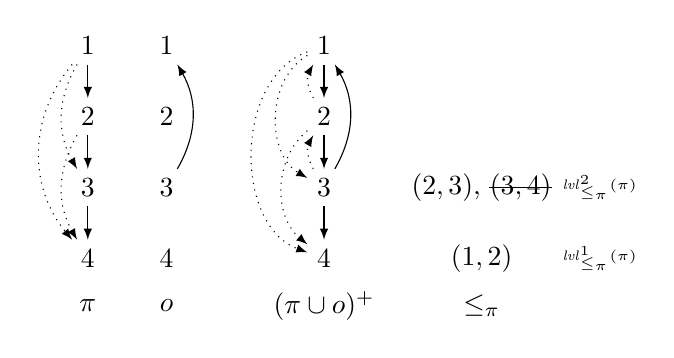
\begin{tikzpicture}
	\node at (0,-1.5){$\p$};
	\node at (0,1.8)(1){$1$};
	\node at (0,0.9)(2){$2$};
	\node at (0,0)(3){$3$};
	\node at (0,-0.9)(4){$4$};
	\path[-latex](1)edge(2)(2)edge(3)(3)edge(4);
	\path[-latex,dotted](1)edge[bend right](3)(2)edge[bend right](4)(1)edge[bend right=40](4);
	
	\node at (1,-1.5){$\o$};
	\node at (1,1.8)(1){$1$};
	\node at (1,0.9)(2){$2$};
	\node at (1,0)(3){$3$};
	\node at (1,-0.9)(4){$4$};
	\path[-latex](3)edge[bend right](1);
	
	\node at (3,-1.5){$(\p\cup\o)^+$};
	\node at (3,1.8)(1){$1$};
	\node at (3,0.9)(2){$2$};
	\node at (3,0)(3){$3$};
	\node at (3,-0.9)(4){$4$};
	\path[-latex](1)edge(2)(2)edge(3)(3)edge(4)(3)edge[bend right](1);
	\path[-latex,dotted]
	(1)edge[bend right=60](3)(2)edge[bend right=50](4)
	(1)edge[bend right=70](4)(2)edge[bend left=30](1)
	(3)edge[bend left=30](2);
	
	\node at (5, -1.5){$\le_\p$};		
	\node at (5,-0.9){$(1,2)$};
	\node at (5,0){$(2,3)$, \sout{$(3,4)$}};
	\node at (6.5,-0.9){\tiny $\lvl^1_{\le_\p}(\p)$};
	\node at (6.5,0){\tiny $\lvl^2_{\le_\p}(\p)$};
	\end{tikzpicture}	
	\caption{
		Preference revision by adding direct comparisons from $\p$ to $\o$, using the preorder $\le_\p$.
		In $\le_\p$ lower means better; the comparison $(3,4)$ is ignored by the addition operator because it
		is not involved in a cycle with $\o$ (and is added at the beginning anyway).
	}
	\label{fig:7-preferences-4-items}
\end{figure}

\begin{xmpl}{}{7-preferences-4-items}
	For 
	%	$V=\{1,2,3,4\}$ and 
	$\p=(1,2,3,4)$, $\o=(3,1)$,
	we obtain that $\dir_\p=\{(1,2),(2,3),(3,4)\}$ .
	Suppose that there is a total preorder $\le_\p$ on $\dir_\p$ according to which
	$(1,2)<_\p (2,3)\approx_\p (3,4)$ (see Figure \ref{fig:7-preferences-4-items}).
	To construct $\p\en\o$, the addition operator starts from
	$\add^0_{\le_\p}(\o)=(\{(3,1)\}\cup\{(1,4),(2,4),(3,4)\})^+$,
	i.e., $\o$ and $\cycfree{\p}{\o}$. At the next step it tries to add $(1,2)$,
	which it can do successfully; at the next step is adds $(2,3)$, after
	which it runs out of comparisons to add.	
\end{xmpl}












\section{Postulates}\label{sec:7-postulates}
We show now that the procedure described in Section \ref{sec:7-semantics}
can be characterized with a set of AGM-like postulates that 
do not reference any concrete revision procedure and are, by themselves,
intuitive enough to provide reasonable constraints on any preference revision operator.
The first two postulates apply to any $\p\in\CHN_V$, $\o\in\SPO_V$ 
and preference revision operator $\en\colon\CHN_V\times\SPO_V\rightarrow\SPO_V$, 
and are as follows:

\begin{description}
	\item[($\ppp{1}$)] $\pi\en\o\in\upper{\o}_\p$.
	\item[($\ppp{2}$)] $\cycfree{\p}{\o}\subseteq \p\en\o$.
\end{description}

Postulates $\ppp{1-2}$ are meant to capture preference revision in its most uncontroversial aspects,
yet they still require some careful unpacking.
Postulate $\ppp{1}$ states that $\p\en\o$ is a $\p$-completion of $\o$,
i.e., a preference order constructed only by adding direct comparisons from $\p$ to $\o$,
and, among other things, ensures that 
($i$) $\p\en\o\in\SPO_V$, 
($ii$) $\o\subseteq\p\en\o$, and
($iii$) $\p\en\o\subseteq(\p\cup\o)^+$. 
In terms of AGM propositional belief change, 
postulate $\ppp{1}$ does the same duty as 
the revision postulates $\ppr{1}$ and $\ppr{3}$
in Section \ref{sec:3-revision},
i.e., it sets limits for the revision result.
However, the closest analogue to postulates $\ppp{1-2}$ are 
enforcement postulates $\ppe{1}$ and $\ppe{3}$, respectively,
in that they require the result to be formed by adding elements to 
the new information, and by requiring the result to be of a certain 
admissible type (refutable in enforcement, an spo here).
Given this, a question emerges as to why not take
condition ($i$)-($iii$) as postulates instead of $\ppp{1}$:
the reason is that, by requiring $\p\en\o$ to be constructed using only direct comparisons 
of $\p$ (in addition to $\o$), postulate $\ppp{1}$ prevents $\p\en\o$ from having opinions on items
over which it had no opinions before, as illustrated in Example \ref{ex:7-P1}.

\begin{xmpl}{}{7-P1}
	For $\p$ and $\o$ as in 
	Example \ref{ex:7-pref-change-3-alternatives-ctd}, 
	note that $\p_4 = \{(3,1),(3,2)\}$
	is such that $\o\subseteq\p_4\subseteq(\p\cup\o)^+$. 
	However, the comparison $(3,2)$ occurs neither 
	in $\p$ nor in $\o$ as a direct comparison, 
	and is entirely unjustified. 
	By contrast, $(3,2)$ in $\p_1=(3,1,2)$ occurs 
	as the result of inference from $(3,1)$, 
	which is added from $\o$,
	and $(1,2)$, which is preserved from $\p$.
\end{xmpl} 

Postulate $\ppp{2}$ says that the cycle-free part of $\p$ with respect to 
$\o$ is to be preserved 
in $\p\en\o$, and is meant to preserve the parts of 
$(\p\cup\o)^+$ that are not up for dispute.
Note that in the case when $(\p\cup\o)^+$ 
does not contain a cycle then $\cycfree{\p}{\o}=(\p\cup\o)^+$,
and $\ppp{2}$ together with $\ppp{1}$ imply that $\p\en\o=(\p\cup\o)^+$: this is the case
when revision is easy, and nothing special needs to be done. In this, postulate $\ppp{2}$
serves the same function as the revision postulate $\ppr{2}$,
but comes closest to enforcement postulate $\ppe{2}$,
in the ideal case, when $\o$ can simply be added to $\p$, results in 
the union of the two structures.

So far we have established that, if there is no conflict between $\p$ and $\o$,
then we can simply add $\o$ to $\p$; and if there is a conflict, then $\en$ must choose
between the direct comparisons of $\p$ involved in the cycle.
This choice, however, must be coherent, in a very precise sense, 
illustrated by Example \ref{ex:7-choice}.

\begin{xmpl}{}{7-choice}
	Consider revising $\p=(1,2,3,4)$ from 
	Example \ref{ex:7-preferences-4-items} by $\o_1=(4,1)$.
	This requires a choice between comparisons $(1,2)$, $(2,3)$ and $(3,4)$:
	assume $(1,2)$ is chosen, suggesting $(1,2)$ is better than $(2,3)$ and $(3,4)$. 
	Suppose, now, that we revise $\p$ by $\o_2=\{(3,1)\}$. This requires a choice
	between $(1,2)$ and $(2,3)$: 
	in accordance with the previous decision, $(1,2)$ should be chosen 
	here as well.
\end{xmpl}

The choice has to reflect an implicit preference order over the direct comparisons of $\p$,
and this is handled by the following postulates, meant to apply to $\p\in\CHN_V$, $\o_1,\o_2\in\SPO_V$
such that $(\o_1\cup\o_2)^+\in\SPO_V$,
and a preference revision operator $\en$:

\begin{description}
	\item[($\ppp{3}$)] $\p\en(\o_1\cup\o_2)^+\subseteq((\p\en\o_1)\cup\o_2)^+$.
	\item[($\ppp{4}$)] If $((\p\en\o_1)\cup\o_2)^+\in\SPO_V$, then $((\p\en\o_1)\cup\o_2)^+\subseteq \p\en(\o_1\cup\o_2)^+$.
\end{description}

There is a similarity between postulates $\ppp{3-4}$ and the revision postulates 
$\ppr{5}$ and $\ppr{6}$ from Section \ref{sec:3-revision},
but the parallel is closest to enforcement postulates $\ppe{5-6}$ from Section \ref{sec:3-enforcement}.
These postulates ensure that the choice between two options is stable and independent of alternatives 
not directly involved. Postulates $\ppp{3-4}$ are meant to ensure the same here:
however, it turns out that in the present context
% of preference revision 
this happens only under a specific set of conditions.

If $\o_1$ and $\o_2$ are spos,
$\o_1$ and $\o_2$ are \emph{coordinated with respect to $\p$} 
if for any $\d\subseteq\cyc{\p}{\o_1}$
such that for every direct comparison $(i,\tightplus{i}{1})\in\delta$, 
neither $(i,\tightplus{i}{1})$ nor $(\tightplus{i}{1},i)$ is in $(\o_1\cup\o_2)^+$, 
it holds that if $(\o_1\cup\d)^+\in\SPO_V$,
then $((\o_1\cup\o_2)^+\cup\d)^+\in\SPO_V$.
In other words, if $\p$ and $\o_1$ form a cycle
and we want to add $\o_2$ as well,
then we look at the direct comparisons in $\p$
that are not directly ruled out by $(\o_1\cup\o_2)^+$,
i.e., such that neitherm them nor their inverses are 
contained in $(\o_1\cup\o_2)^+$.
The property of coordination says that 
if we can consistently add some of these 
comparisons to $\o_1$,
then we can also add them to $(\o_1\cup\o_2)^+$. 
Intuitively, coordination means that adding
extra information $\o_2$ does not step on $\o_1$'s toes 
by rendering unviable any
comparisons that were previously viable.
The following example makes this clearer.

\begin{figure}\centering
	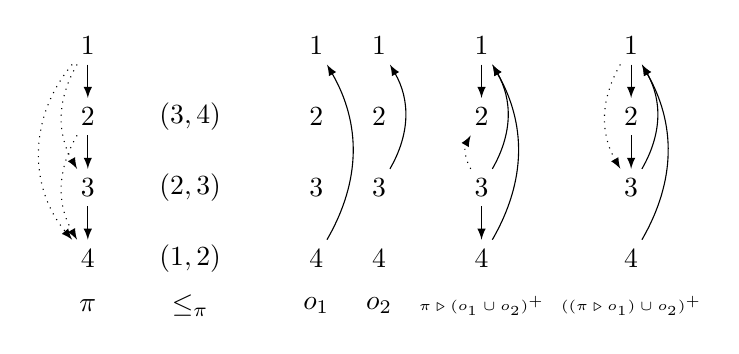
\begin{tikzpicture}
	\node at (0,-1.5){$\p$};
	\node at (0,1.8)(1){$1$};
	\node at (0,0.9)(2){$2$};
	\node at (0,0)(3){$3$};
	\node at (0,-0.9)(4){$4$};
	\path[-latex](1)edge(2)(2)edge(3)(3)edge(4);
	\path[-latex,dotted](1)edge[bend right](3)(2)edge[bend right](4)(1)edge[bend right=40](4);
	
	\node at (1.3,-1.5){$\le_\p$};		
	\node at (1.3,-0.9){$(1,2)$};
	\node at (1.3,0){$(2,3)$};
	\node at (1.3,0.9){$(3,4)$};
	%%	\node at (6.5,-0.9){\tiny $\lvl^1_{\le_\p}(\p)$};
	%%	\node at (6.5,0){\tiny $\lvl^2_{\le_\p}(\p)$};
	
	\node at (2.9,-1.5){$\o_1$};
	\node at (2.9,1.8)(1){$1$};
	\node at (2.9,0.9)(2){$2$};
	\node at (2.9,0)(3){$3$};
	\node at (2.9,-0.9)(4){$4$};
	\path[-latex](4)edge[bend right](1);
	
	\node at (3.7,-1.5){$\o_2$};
	\node at (3.7,1.8)(1){$1$};
	\node at (3.7,0.9)(2){$2$};
	\node at (3.7,0)(3){$3$};
	\node at (3.7,-0.9)(4){$4$};
	\path[-latex](3)edge[bend right](1);
	
	\node at (5,-1.5){\tiny $\p\en(\o_1\cup\o_2)^+$};
	\node at (5,1.8)(1){$1$};
	\node at (5,0.9)(2){$2$};
	\node at (5,0)(3){$3$};
	\node at (5,-0.9)(4){$4$};
	\path[-latex](4)edge[bend right](1);
	\path[-latex](3)edge[bend right](1);
	\path[-latex](1)edge(2)(3)edge[dotted,bend left](2);
	\path[-latex](3)edge(4);
	
	\node at (6.9,-1.5){\tiny $((\p\en\o_1)\cup\o_2)^+$};
	\node at (6.9,1.8)(1){$1$};
	\node at (6.9,0.9)(2){$2$};
	\node at (6.9,0)(3){$3$};
	\node at (6.9,-0.9)(4){$4$};
	\path[-latex](4)edge[bend right](1)(1)edge(2)(2)edge(3)(1)edge[dotted, bend right](3);
	\path[-latex](3)edge[bend right](1);
	\end{tikzpicture}	
	\caption{
		Postulates $\ppp{3-4}$ are satisfied only if $\o_1$ and $\o_2$ are coordinated with respect to $\p$.
		}
	\label{fig:7-non-coordination}
\end{figure}

\begin{xmpl}{}{7-coordination}
	Take $\p=(1,2,3,4)$ and $\o_1=(4,1)$, $\o_2=(3,1)$.
	The direct comparisons of $\p$ that are involved in a cycle
	with $\o_1$ are $\cyc{\p}{\o_1}=\{(1,2),(2,3),(3,4)\}$,
	so that revision by $\o_1$ requires making a choice between $(1,2)$, $(2,3)$ and $(3,4)$.
	Notice that neither of $(1,2)$, $(2,3)$ and $(3,4)$ is directly ruled out by 
	$(\o_1\cup\o_2)^+$: we have, for instance, that $(1,2)\notin(\o_1\cup\o_2)^+$
	and $(2,1)\notin(\o_1\cup\o_2)^+$, and the same holds for $(2,3)$ and $(3,4)$.
	The significance of this is that adding $\o_2$ to $\o_1$ still 
	makes the choice over which comparisons to keep be between 
	$(1,2)$, $(2,3)$ and $(3,4)$.
	
	However, consider the set
	$\d=\{(1,2),(2,3)\}$. We have that 
	$(\o_1\cup\d)^+\in\SPO_V$, but $((\o_1\cup\o_2)^+\cup\d)^+\notin\SPO_V$,
	meaning that $\o_1$ and $\o_2$ are not coordinated with respect to $\p$.
	In other words, whereas with $\o_1$ we can add $(1,2)$ and $(2,3)$ together,
	with $\o_1$ and $\o_2$ we cannot add them anymore.
	This, then, makes it possible to add $(3,4)$, irrespective of where it 
	is in the preorder on comparisons.
	
	At the same time, for the preorder $\le_\p$ in Figure \ref{fig:7-non-coordination}
	and the revision operator $\en$ induced by it,
	we have that $(3,4)\in\p\en(\o_1\cup\o_2)^+$, but $(3,4)\notin((\p\en\o_1)\cup\o_2)^+$,
	i.e., postulate $\ppp{3}$ is not satisfied.
	The two facts are related, as the addition of $\o_2$ tampers with the choice problem:
	though we can still add either one of the three comparisons, 
	as mentioned above,
	we cannot add $(1,2)$ and $(2,3)$
	together anymore, which in turn means that 
	$(3,4)$ can be added regardless of its position in $\le_\p$. 
\end{xmpl}

The significance of coordination, as the following theorem shows,
is that it is needed in order for postulates $\ppp{3-4}$ to be effective at 
ensuring that choice across different types of incoming preferences
is coherent.

\begin{thm}{}{7-P34-coordination}
	If $\as\colon\CHN_V\rightarrow\TPRE_{V\times V}$ 
	is a preference assignment and $\en^\as$ 
	is the $\as$-induced revision operator,
	then, 
	$\en^\as$ satisfies postulates $\ppp{3-4}$
	if and only if, 
	for any $\p\in\CHN_V$ and $\o_1,\o_2\in\SPO_V$, 
	it holds that $\o_1$ and $\o_2$ are coordinated with respect to $\p$.
\end{thm}
\begin{prf*}{}{}%
	(``$\Leftarrow$'')
	Take $\o_1,\o_2\in\SPO_V$ that are coordinated with respect to $\p$.
	We will show that, for any preorder $\le_\p$ on $\dir_\p$,
	the $\as$-induced revision operator $\en^\as$ satisfies postulates $\ppp{3-4}$.
	Since 
	%	the statement is trivially satisfied 
	$\en^\as$ satisfies postulates $\ppp{3-4}$ trivially
	if $(\p\cup\o_1)^+\in\SPO_V$,
	we look at the case when $\cyc{\p}{\o_1}\neq\emptyset$,
	i.e., when $(\p\cup\o_1)^+$ contains a cycle.
	
	For postulate $\ppp{3}$, assume there is a 
	comparison $c^\star\in\add^\ast_{\le_\p}(\o_1\cup\o_2)^+$
	such that $c^\star\notin(\add^\ast_{\le_\p}(\o_1)\cup\o_2)^+$.
	If $c^\star\in(\o_1\cup\o_2)^+$ then a contradiction follows immediately.
	We thus have to look 
	at the case when $c^\star\notin(\o_1\cup\o_2)^+$, which contains two subcases 
	of its own.

	\emph{Case 1}. 
	If $c^\star\in\dir_\p$, then by our assumption 
	we have that $c^\star\in\cyc{\p}{\o_1}$, i.e., 
	$c^\star$ is involved in some cycle with $\o_1$.
	From $c^\star\notin\add^\ast_{\le_\p}(\o_1)$ 
	we infer that there must be a set $\d\subseteq\dir_\p$
	of direct comparisons of $\p$ 
	that precede $c^\star$ in $\le_\p$, are added to $\o_1$ before it, 
	and prevent $c^\star$ itself from being added.
	In particular, this means that $(\o_1\cup\d)^+\in\SPO_V$, 
	but $((\o_1\cup\d)^+\cup\{c^\star\})^+\notin\SPO_V$. 
	At the same time, we know that $c^\star\in\add^\ast_{\le_\p}(\o_1\cup\o_2)^+$,
	i.e., $c^\star$ can be consistently added to $(\o_1\cup\o_2)^+$.
	Note that this happens after all the comparisons in $\d$, which precede it in $\le_\p$,
	have been considered as well.
	This implies that not all of the comparisons in $\d$ can be added to $(\o_1\cup\o_2)^+$,
	since if they could, then the cycle formed with $\o_1$, $\d$ and $c^\star$ would be reproduced here
	as well. 
	If not all of the comparisons in $\d$ can be added to $(\o_1\cup\o_2)^+$,
	this must be because $((\o_1\cup\o_2)^+\cup\d)^+$ contains a cycle,
	i.e., $((\o_1\cup\o_2)^+\cup\d)^+\notin\SPO_V$.
	This now contradicts the fact that $\o_1$ and $\o_2$ are coordinated with respect to $\p$.
	
	\emph{Case 2}. 
	If $c^\star$ is not a direct comparison of $\p$, then it is inferred 
	by transitivity using at least one direct comparison of $\p$ added previously. 
	We apply the reasoning in Case 1 to these direct comparisons to show that they are in 
	$(\add^\ast_{\le_\p}(\o_1)\cup\o_2)^+$, which implies the conclusion as well.
	%	 that 
	%	$c^\star\in(\add^\ast_{\le_\p}(\o_1)\cup\o_2)^+$ as well.	
	
	For postulate $\ppp{4}$, take $c^\star\in(\add^\ast_{\le_\p}(\o_1)\cup\o_2)^+$
	and assume $c^\star\notin\add^\ast_{\le_\p}(\o_1\cup\o_2)^+$.
	As before, the non-obvious case is when $c^\star\notin(\o_1\cup\o_2)^+$.
	If $c^\star\in\dir_\p$, 
	then from the assumption that $c^\star\notin\add^\ast_{\le_\p}(\o_1\cup\o_2)^+$
	we conclude that there is a set $\d\subseteq\cyc{\p}{\o_1}$ of comparisons 
	that precede $c^\star$ in $\le_\p$,
	are added to $(\o_1\cup\o_2)^+$ before it and, in concert with $(\o_1\cup\o_2)^+$, 
	block $c^\star$ from being added, i.e., 
	% such that
	$((\o_1\cup\o_2)^+\cup\d)^+\in\SPO_V$ but
	$((\o_1\cup\o_2)^+\cup\d')^+\notin\SPO_V$,
	where $\d'=\d\cup\{c_\star\}$.
	From the second to last result 
	we infer that $\d$ can be added consistently to $(\o_1\cup\o_2)^+$
	and, since we have that $c^\star\in(\add^\ast_{\le_\p}(\o_1)\cup\o_2)^+$ as well,
	we obtain that 
	and $c^\star$ can be added consistently to $\o_1$.
	In other words, it holds that 
	$(\o_1\cup\d')^+\in\SPO_V$,
	which contradicts the coordination assumption.
	%	
	%	Together with the previous result this contradicts the fact that $o_1$ and $\o_2$ are coordinated 
	%	with respect to $\p$.
	The case when $c^\star\notin(\o_1\cup\o_2)^+$ is 
	treated analogously as for postulate $\ppp{3}$.
	
	
	(``$\Rightarrow$'')
	Assume that there are $\o_1,\o_2\in\SPO_V$ not coordinated with respect to $\p$,
	i.e., there exists a set $\delta\subseteq\cyc{\p}{\o_1}$ of direct comparisons of $\p$
	that are involved in a cycle with $\o_1$ and are such that
	$(\o_1\cup\d)^+\in\SPO_V$ and $((\o_1\cup\o_2)^+\cup\d)^+\notin\SPO_V$.
	Additionally, we have that neither of the comparisons in $\delta$, 
	or their inverses, are in $(\o_1\cup\o_2)^+$.
	%	Since the comparisons in $\d$ can all be added consistently to $\o_1$,
	We infer that there must exist a comparison $c^\star\in(\cyc{\p}{\o_1}\setminus\d)$
	that completes the cycle. 
	We will show that there exists a preorder $\le_\p$ 
	such that the revision operator	induced by it does not satisfy $\ppp{3}$.
	Take a preorder $\le_\p$ on $\dir_\p$ that arranges the elements 
	of $\d$ in a linear order at the bottom of $\le_\p$, 
	i.e., such that $c_j<_\p c_l$, for any $c_j\in\d$ and $c_l\notin\d$,
	and $c^\star$ the maximal element in $\le_\p$,
	i.e., $c_j<_\p c^\star$, for any $c_j\in\d$.
	This implies, in particular, that $c_j<_\p c^\star$, for any $c_j\in\d$.
	Note, now, that $c^\star\in\add_{\le_\p}^\ast(\o_1\cup\o_2)^+$: 
	this is because, by assumption, not all of the comparisons in 
	$\d$ can be added to $(\o_1\cup\o_2)^+$,
	and this makes it possible for $c^\star$ to be added.
	On the other hand, $c^\star\notin(\add^\ast_{\le_\p}(\o_1)\cup\o_2)^+$:
	this is because here we can, again by assumption, consistently add $\d$ to $\o_1$ and,
	since $c^\star$ is the last in line to be added, the inevitability
	of creating a cycle with $\d$ and the rest of the comparisons of $\o_1$
	makes it impossible to do so consistently. 
	We obtain that $c^\star\in\add_{\le_\p}^\ast(\o_1\cup\o_2)^+$ but 
	$c^\star\notin(\add^\ast_{\le_\p}(\o_1)\cup\o_2)^+$, i.e., postulate $\ppp{3}$ is not satisfied.
	Concurrently, there will be a comparison in $\d$ that occurs in $(\add^\ast_{\le_\p}(\o_1)\cup\o_2)^+$
	that does not make it into $\add^\ast_{\le_\p}(\o_1\cup\o_2)^+$, 
	showing that $\ppp{4}$ is not satisfied either.
\end{prf*}

Theorem \ref{thm:7-P34-coordination} shows that coordination is needed in order to make
sure that postulates $\ppp{3-4}$ work, and we will henceforth assume that $\o_1$ and $\o_2$ 
are coordinated with respect to $\p$ whenever we apply these postulates.








\section{Preference revision as choice over comparisons}\label{sec:7-representation}
We show now that the procedure described in 
Section \ref{sec:7-semantics} is characterized
by the postulates introduced 
in Section \ref{sec:7-postulates}, under the restrictions
established through Theorem \ref{thm:7-P34-coordination}.
Theorem \ref{thm:7-repr-ties-lr} shows that the procedure in 
Section \ref{sec:7-semantics} 
yields preference revision operators that satisfy postulates $\ppp{1-4}$.
%under the restrictions considered previously.

\begin{thm}{}{7-repr-ties-lr}
	If $\as\colon\CHN_V\rightarrow\TPRE_{V\times V}$ is a preference assignment,
	then the revision operator $\en^\as$ induced by it satisfies postulates $\ppp{1-4}$,
	for any $\p\in\CHN_V$ and $\o,\o_1,\o_2\in\SPO_V$ such that $\o_1$, $\o_2$ are coordinated 
	with respect to $\p$.
\end{thm}
\begin{prf*}{}{}%
	Satisfaction of postulates $\ppp{1-2}$ is straightforward.
	For $\ppp{1}$, since at every step $\add^i_{\le_\p}$ 
	selects some direct comparisons in $\p$ to add to $\o$,
	the end result satisfies the condition for being in $\upper{\o}_\p$.
	For $\ppp{2}$, note that 
	$\cf(\p\cup\o)^+\subseteq\add^0_{\le_\p}(\o)\subseteq\add_{\le_\p}^\ast(\o)$.
	Since $\o_1$ and $\o_2$ are assumed to be coordinated with respect to $\p$, 
	satisfaction of postulates $\ppp{3-4}$ 
	is guaranteed by Theorem \ref{thm:7-P34-coordination}.	
\end{prf*}

For the converse, we want to show that any preference revision operator satisfying $\ppp{1-4}$
can be rationalized using a preference assignment.
To that end, we will construct the preorder $\le_\p$ from binary comparisons,
but we must first figure out how to compare two direct comparisons $\drc{k}$ and $\drc{l}$.
This is done by creating a situation where we cannot add both and hence one has to be given up.
We will use a special type of preference order to induce a choice between these comparisons.
If $\p\in\CHN_V$ and $\drc{k},\drc{l}\in\dir_\p$,
the \emph{choice inducing preference $\o_{k,l}$ for $\drc{k}$ and $\drc{l}$} is
defined as $\o_{k,l}=\{(\tightplus{k}{1},l),(l{+}1, k)\}$.
%added convention that if $\tightplus{k}{1} = l$, then the problem becomes of
%inducing a choice between $\drc{k}$ and $(\tightplus{k}{1},\tightplus{k}{2})$, and the choice inducing preference
%is $\o_{k,\tightplus{k}{1}}=\{(\tightplus{k}{2},k)\}$.

\begin{figure}\centering
	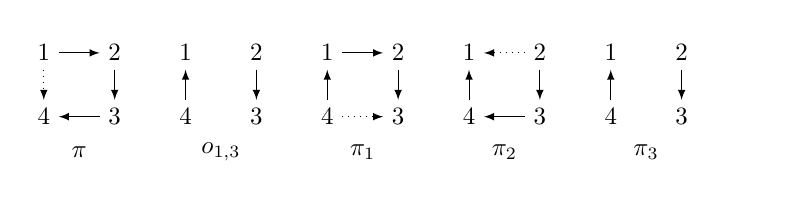
\begin{tikzpicture}
	\scalebox{0.9}{
		\node at (0.5,-0.5){$\p$};
		\node at (0,0.9)(1){$1$};
		\node at (1,0.9)(2){$2$};
		\node at (1,0)(3){$3$};
		\node at (0,0)(4){$4$};
		\path[-latex] (1)edge(2)(3)edge(4)(2)edge(3)(1)edge[dotted](4);
		
		\node at (2.5,-0.5){$\o_{1,3}$};
		\node at (2,0.9)(1){$1$};
		\node at (3,0.9)(2){$2$};
		\node at (3,0)(3){$3$};
		\node at (2,0)(4){$4$};
		\path[-latex] (2)edge(3)(4)edge(1);
		
		\node at (4.5,-0.5){$\p_1$};
		\node at (4,0.9)(1){$1$};
		\node at (5,0.9)(2){$2$};
		\node at (5,0)(3){$3$};
		\node at (4,0)(4){$4$};
		\path[-latex] (1)edge(2)(2)edge(3)(4)edge(1)(4)edge[dotted](3);
		
		\node at (6.5,-0.5){$\p_2$};
		\node at (6,0.9)(1){$1$};
		\node at (7,0.9)(2){$2$};
		\node at (7,0)(3){$3$};
		\node at (6,0)(4){$4$};
		\path[-latex] (4)edge(1)(2)edge(3)(3)edge(4)(2)edge[dotted](1);
		
		\node at (8.5,-0.5){$\p_3$};
		\node at (8,0.9)(1){$1$};
		\node at (9,0.9)(2){$2$};
		\node at (9,0)(3){$3$};
		\node at (8,0)(4){$4$};
		\path[-latex] (4)edge(1)(2)edge(3);
	}
	\end{tikzpicture}
	\caption{
		Revision of $\p$ by $o_{1,3}$ forces a choice between direct comparisons
		$(1,2)$ and $(3,4)$: since keeping both $(1,2)$ and $(3,4)$ is not possible, 
		at least one of them, potentially both, must be discarded.
		Depending on the choice made, possible results are $\p_1$, $\p_2$ and $\p_3$.
	}
	\label{fig:7-choice-inducing-preference}
\end{figure}

\begin{xmpl}{}{7-choice-inducing-preference}
	To induce a choice between direct comparisons 
	$(1,2)$ and $(3,4)$ in Figure \ref{fig:7-choice-inducing-preference}, revise by 
	$\o_{1,3}=\{(2,3),(4,1)\}$.
	Note that effectiveness of this maneuver hinges on the choice 
	being confined to the direct comparisons of $\p$:
	if inferred comparisons were allowed to be part of the choice, 
	$\o_{1,3}$ loses its power to discriminate between $(1,2)$ and $(3,4)$:
	if, for instance, $(1,3)$ and $(2,4)$ are chosen, then $(2,1)$ and $(4,3)$ 
	have to be inferred, leaving no space for a choice between $(1,2)$ and $(3,4)$,
	i.e., $\o_{1,3}$ would tell us nothing about the implicit preference between $(1,2)$ and $(3,4)$.
	We can also see that comparison of $(1,2)$ and $(2,3)$ is done by revising by $(3,1)$.	
\end{xmpl}

If $\drc{k},\drc{l}\in\dir_\p$
and $\en$ is a preference revision operator, then the 
\emph{revealed order $\le^\en_\p$ between $\drc{k}$ and $\drc{l}$} is defined as:
$$
	\drc{k}\le^\en_\p \drc{l}~\textnormal{if}~\drc{l}\notin\p\en\o_{k,l}.
$$
Intuitively, $\drc{l}$ being discarded from $\p\en\o_{k,l}$ signals 
that it is considered less
important than $\drc{k}$. 

\begin{figure}\centering
	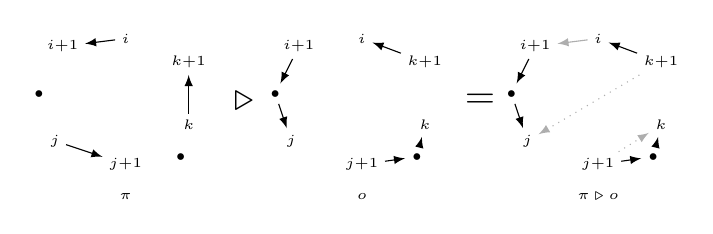
\begin{tikzpicture}\tiny
	\node at (0,-1.3){$\p$};
	\node at (0,0.7)(1){$i$};
	\node at (-0.8, 0.6)(2){$i{+}1$};
	\node at (-1.1,0)(3){$\bullet$};
	\node at (-0.9, -0.6)(4){$j$};
	\node at (0,-0.9)(5){$j{+}1$};
	\node at (0.7,-0.8)(6){$\bullet$};
	\node at (0.8,-0.4)(7){$k$};
	\node at (0.8,0.4)(8){$\tightplus{k}{1}$};
	\path[-latex] (1)edge(2)(4)edge(5)(7)edge(8);
	
	\node at (1.5,-0.1){\Large $\en$};
	
	\node at (3,-1.3){$\o$};
	\node at (3,0.7)(1){$i$};
	\node at (2.2, 0.6)(2){$i{+}1$};
	\node at (1.9,0)(3){$\bullet$};
	\node at (2.1, -0.6)(4){$j$};
	\node at (3,-0.9)(5){$j{+}1$};
	\node at (3.7,-0.8)(6){$\bullet$};
	\node at (3.8,-0.4)(7){$k$};
	\node at (3.8,0.4)(8){$\tightplus{k}{1}$};
	\path[-latex] (2)edge(3)(3)edge(4)(5)edge(6)(6)edge(7)(8)edge(1);
	
	\node at (4.5,-0.1){\Large $=$};
	
	\node at (6,-1.3){$\p\en\o$};
	\node at (6,0.7)(1){$i$};
	\node at (5.2, 0.6)(2){$i{+}1$};
	\node at (4.9,0)(3){$\bullet$};
	\node at (5.1, -0.6)(4){$j$};
	\node at (6,-0.9)(5){$j{+}1$};
	\node at (6.7,-0.8)(6){$\bullet$};
	\node at (6.8,-0.4)(7){$k$};
	\node at (6.8,0.4)(8){$\tightplus{k}{1}$};
	\path[-latex] (2)edge(3)(3)edge(4)(5)edge(6)(6)edge(7);
	\path[-latex] (1)edge[gray!60](2)(8)edge(1);
	\path[-latex] (8)edge[dotted,gray!60](4)(5)edge[dotted,gray!60](7);
	\end{tikzpicture}
	\caption{
		To show that $\le_\p^\en$ is transitive,
		we show first that $\drc{k}\notin\p\en\o$.
		Bullets indicate other potential items in $\p$;
		faded arrows indicate comparisons that may not be in $\p\en\o$,
		but can be consistently added to it.
	}
	\label{fig:7-acyclic-proof}
\end{figure}


\begin{lem}{}{7-revealed-preference-relation-transitive}
	If $\en$ satisfies postulates $\ppp{1-4}$, 
	then the revealed preference relation $\le_\p^\en$	
	is transitive.
\end{lem}
\begin{prf*}{}{}%	
	Take $\p\in\CHN_V$ and $\drc{i}, \drc{j}, \drc{k}\in\dir_\p$
	such that $\drc{i}\le^\en_\p\drc{j}\le^\en_\p\drc{k}$
	(we can assume that $i<j<k$).
	To show that $\drc{i}\le^\en_\p\drc{j}$,
	take $\o\in\SPO_V$ that contains all direct comparisons in $\p$
	up to $k$, except $\drc{i}$, $\drc{j}$ and $\drc{k}$, 
	plus the comparison $(\tightplus{k}{1},i)$. 
	In other words,
	$\o$ is such that if $\drc{i}$, $\drc{j}$ and $\drc{k}$ were added to it,
	a cycle would form.
	The first step involves showing that $\drc{k}\notin\p\en\o$.	
	To see why this is the case, 
	note first that, 
	by design, not all of $\drc{i}$, $\drc{j}$ and $\drc{k}$ can be in $\p\en\o$,
	i.e., at least one of them must be left out. 
	We now do a case analysis
	to show that,
	either way, $\drc{k}$ ends up being left out.
	
	\emph{Case 1}. If $\drc{k}\notin\p\en\o$, the conclusion is immediate.
	
	\emph{Case 2}. If $\drc{j}\notin\p\en\o$, then we can safely add $\drc{i}$ to $\p\en\o$:
	this is because the inference of 
	the opposite comparison, i.e., 
	$(i{+}1,i)$, can be done
	only by adding all comparisons on the path from $i{+}1$ to $i$, and the absence
	of $\drc{j}$ means this inference is blocked. Using $\ppp{3-4}$ we can now conclude that
	$((\p\en\o)\cup\{\drc{i}\})^+=\p\en(\o\cup\{\drc{i}\})^+$
	(see Figure \ref{fig:7-acyclic-proof}).
	Note, we can separate $\o\cup\{\drc{i}\}$ into $\o_{j,k}=\{(k{+}1,j), (j{+}1,k)\}$ and 
	all the comparisons on the path from $k{+}1$ to $j$, plus the comparisons on the path
	from $j{+}1$ to $k$. Call this latter preference $\o'$.
	We thus have that $(\o\cup\{\drc{i}\})^+=(\o_{j,k}\cup\o')^+$
	and, applying $\ppp{3}$, we obtain that:
	$$
	\p\en(\o\cup\{\drc{i}\})^+ = \p\en(\o_{j,k}\cup\o')^+\subseteq((\p\en\o_{j,k})\cup\o')^+.
	$$		
	Since, by definition, $\drc{k}\notin\p\en\o_{j,k}$ and $\drc{k}\notin\o'$,
	It follows that $\drc{k}\notin\p\en(\o\cup\{\drc{i}\})^+$,
	then $\drc{k}\notin((\p\en\o)\cup\{\drc{i}\})^+$,
	and, finally, that $\drc{k}\notin\p\en\o$.
	
	\emph{Case 3}. 
	If $\drc{i}\notin\p\en\o$, then we can safely add $\drc{k}$ to $\p\en\o$
	and, by reasoning similar to above, show that 
	$\drc{j}\notin\p\en\o$. Here we invoke Case 2.
	
	With the fact that $\drc{k}\notin\p\en\o$ in hand, 
	we can add $\drc{j}$ to $\p\en\o$ (by reasoning similar to above),
	because the path from $j{+1}$ to $j$ in $\p\en\o$ is blocked by the absence of $\drc{k}$.
	Using postulates $\ppp{3-4}$, we conclude that:
	% $$
	% ((\p\en\o)\cup\{\drc{j}\})^+ =\p\en(\o\cup\{\drc{j}\})^+
	% = \p\en(\{(i{+}1,\dots,k),(k{+1},i)\})^+
	% =((\p\en\o_{i,k})\cup\{(i{+}1,\dots,k)\})^+.	
	% $$
		\begin{align*}
			((\p\en\o)\cup\{\drc{j}\})^+ &=\p\en(\o\cup\{\drc{j}\})^+\\
			&= \p\en(\{(i{+}1,\dots,k),(k{+1},i)\})^+\\
			&=((\p\en\o_{i,k})\cup\{(i{+}1,\dots,k)\})^+.
		\end{align*}
	Since $\drc{k}\notin((\p\en\o)\cup\{\drc{j}\})^+$, we conclude that 
	$\drc{k}\notin\p\en\o_{i,k}$,
	which implies that $\drc{i}\le^\en_\p\drc{k}$.
\end{prf*}

Lemma \ref{lem:7-revealed-preference-relation-transitive} 
is crucial for the following 
representation result.

\begin{thm}{}{7-repr-ties-rl}
	If $\en$ is a revision operator satisfying postulates $\ppp{1-4}$,
	for any $\p\in\CHN_V$ and $\o,\o_1,\o_2\in\SPO_V$ such that $\o_1$, $\o_2$ are coordinated 
	with respect to $\p$,
	then there exists a preference assignment $\as$ 
	such that $\en$ is the $\as$-induced revision operator.
\end{thm}
\begin{prf*}{}{}%
	For any $\p\in\CHN_V$, take $\le_\p$ to be the revealed preference relation $\le^\en_\p$.
	By Lemma \ref{lem:7-revealed-preference-relation-transitive}, we know that 
	$\le_\p$ is transitive, 
	so the only thing left to is show is that $\p\en\o = \add^\ast_{\le_\p}(\o)$.
	We do this in two steps.
	
	(``$\subseteq$'') 
	For one direction, 
	Take $(j,k)\in\p\en\o$ and suppose 
	$(j,k)\notin\add^\ast_{\le_\p}(\o)$.
	Clearly, it cannot be the case that $(j,k)\in\o$, so we conclude that $(j,k)$
	is either a direct comparison of $\p$, or is inferred by transitivity using direct comparisons in $\p$
	and $\o$. 	
	
	\emph{Case 1}. If $(j,k)\in\dir_\p$, then we can write $(j,k)$ as $\drc{j}$,
	Suppose that $\drc{j}$ is on level $i$ of $\dir_\p$: this means that if $\drc{j}$ does not get added to 
	$\add^\ast_{\le_\p}(\o)$ at step $i$, then, since it cannot be inferred by transitivity,
	it does not get added at all. The fact that $\drc{j}\notin\add^\ast_{\le_\p}(\o)$ thus means that
	$\drc{j}$ forms a cycle with some comparisons in $\o$ and comparisons in $\p$ on levels $l\le i$.
	First, note that $\drc{j}$ cannot form a cycle with elements of $\o$ only, since that would imply
	that $(j{+}1,j)\in\o$ and that would exclude the possibility that $\drc{j}\in\p\en\o$.
	Thus, at least one other comparison in the cycle must come from $\p$.
	We can state, now, that, since $(j{+}1,j)\in\p\en\o$, then at least one of these comparisons 
	must be absent in $\p\en\o$,
	i.e., there exists a direct comparison $\drc{k}\in\dir_\p$ such that $\drc{k}\in\lvl^j_{\le_\p}(\p)$,
	for some $j\le i$, 
	$\drc{k}\notin\p\en\o$ and $\drc{j}$, $\drc{k}$, plus some other comparisons in $\o$ and $\p$ form a cycle.
	This means that it is safe to add $\o'$ to $\p\en\o$, where $\o'$ contains all comparisons on the path from $\tightplus{k}{1}$ to $j$,	plus the comparison on the path from $j{+}1$ to $k$.
	We can rewrite $\o'$ by separating out $(\tightplus{k}{1},j)$ and $(j{+}1,k)$, i.e., $\o'=(\o_{j,k}\cup\o')^+$.
	Applying postulates $\ppp{3-4}$, we now get that
	\begin{align*}
	((\p\en\o)\cup\o')^+ &= \p\en(\o\cup\o')^+\\
					   &= \p\en(\o_{j,k}\cup\o')^+\\
					   &\subseteq ((\p\en\o_{j,k})\cup\o')^+.						   
	\end{align*}
	Using the assumption that $\drc{j}\in\p\en\o$ and the fact that $\drc{j}\notin{\o'}$, 
	we can thus infer that $\drc{j}\in\p\en\o_{j,k}$.
	This, in turn, implies that $\drc{j}<_\p\drc{k}$ and hence $\drc{j}$ belongs to 
	a lower level of $\dir_\p$ than $\drc{k}$: but this contradicts the conclusion drawn earlier
	that $\drc{k}$ belongs to a level $l\le i$, where $i$ is the level of $\drc{j}$. 

	\emph{Case 2}. 
	If $(j,k)$ is not a direct comparison of $\p$, then it is inferred from some direct
	comparisons of $\p$ that end up in $\p\en\o$,
	together with comparisons in $\o$. We can now apply the reasoning from Case 1
	to the direct comparisons of $\p$ that go into inferring $(j,k)$, to show that they must be in 
	$\add^\ast_{\le_\p}(\o)$. 
	This, in turn, implies that $(j,k)$ will be in $\add^\ast_{\le_\p}(\o)$
	as well.
	
	The reasoning for the other direction is similar.
\end{prf*}


Theorems \ref{thm:7-repr-ties-lr} and \ref{thm:7-repr-ties-rl} 
describe preference revision operators that 
rely on total preorders $\le_\p$ on $\dir_\p$, where a tie between two direct comparisons 
means that if they cannot both be added, then they are both passed over.
We can eliminate this indeciseveness by using \emph{linear} orders on $\dir_\p$ instead of
preorders: this ensures that any two direct comparisons of $\p$ can be clearly ranked with respect
to each other, and that a revision operator is always in a position to choose among them.
On the postulate site, linear orders can be characterized by tightening the notion
of a $\p$-completion and, with it, postulate $\ppp{1}$.
Thus, a \emph{decisive $\p$-completion of $\o$} is
defined as: 
$$
\upperd{\o}_\p \defeq \{(\o\cup\d)^+\in\SPO_V\mid\emptyset\subset\d\subseteq\dir_\p\}.
$$
The decisive version of $\ppp{1}$ is written, for any $\p\in\CHN_V$ and $\o\in\SPO_V$, as:
\begin{description}
	\item[($\ppp{\mathsf{D}}$)] $\p\en\o\in\upperd{\o}_\p$. 
\end{description}

A \emph{decisive preference assignment $\as$} is a 
function $\as\colon\CHN_V\rightarrow\CHN_{V\times V}$ mapping every $\p\in\CHN_V$ to a linear preorder $<_\p$ on $\dir_\p$. We can now show the following result.

\begin{thm}{}{7-repr-decisive}
	A revision operator $\en$ satisfies postulates $\ppp{\mathsf{D}}$ and $\ppp{2-4}$ 
	if and only if
	there exists a decisive preference assignment $a$ such that, for any $\p\in\CHN_V$
	and $\o,\o_1,\o_2\in\SPO_V$ such that $\o_1$, $\o_2$ are coordinated 
	with respect to $\p$, $\en$ is the $\as$-induced preference revision operator.
\end{thm}
\begin{prf*}{}{}%
	The proofs for Theorems \ref{thm:7-repr-ties-lr} and \ref{thm:7-repr-ties-rl} 
	work here with minimal adjustments.
	Note that when choosing between two direct comparisons, postulate $\ppp{\mathsf{D}}$ does not allow $\en$ 
	to be indifferent anymore. This means that the revealed preference relation on $\dir_\p$ ends up being linear.
\end{prf*}






\section{Concrete preference revision operators}\label{sec:7-concrete-operator}
Theorems \ref{thm:7-repr-ties-lr}, 
\ref{thm:7-repr-ties-rl} and \ref{thm:7-repr-decisive} articulate an important lesson:
preference revision performed in a principled manner, 
i.e., in accordance with $\ppp{1-4}$ or $\ppp{\mathsf{D}}$ and $\ppp{2-4}$,
involves having preferences over comparisons.
Thus, to obtain concrete operators one must look at ways of 
ranking the comparisons in a preference $\p$.
We present here two simple solutions.

The \emph{trivial assignment $\as^\mathrm{t}$}
and the \emph{lexicographic assignment $\as^\mathrm{lex}$} 
are defined by taking $\drc{i}\approx^\mathrm{t}_\p\drc{j}$
and, respectively,
$
\drc{i}<^\mathrm{lex}_\p\drc{j}
$ if $i<j$,
for any $\p\in\CHN_V$ and $\drc{i},\drc{j}\in\p$,
These assignments induce the \emph{trivial} and \emph{lexicographic} operators $\en^\mathrm{t}$ and $\en^\mathrm{lex}$, respectively.
Note that $\le_{\p}^\mathrm{t}$ is a preorder and $<^\mathrm{lex}_\p$ is a linear order, prompting the following result.

\begin{prp}{}{7-trivial-lex}
	The operators $\en^\mathrm{t}$ and $\en^\mathrm{lex}$ satisfy postulates $\ppp{1-4}$
	and $\ppp{\mathsf{D}}$ and $\ppp{2-4}$, respectively.	
\end{prp}

\begin{xmpl}{}{7-trivial-lexi}
	For $\p$ and $\o$ as in Example \ref{ex:7-pref-change-3-alternatives-ctd}, 
	we obtain that
	$\p\en^\mathrm{t}\o=(31)$ and $\p\en^\mathrm{lex}\o=(312)$.
\end{xmpl}













\section{Related work}\label{sec:7-rw}
Our work comes on the heels of existing research, 
but manages to carve its own niche in an otherwise 
populated landscape.
Contrary to some previous work labeled as revision of preferences \cite{Bradley07,LangT08,Liu11}, 
we do not look at changes in preferences elicited by a change in beliefs: 
not because this is not an interesting topic, but because we are more interested 
in the mechanism of preference change independently of any other cognitive operations 
running at the same time.

More involved work \cite{CadilhacALB15} describe preference change when 
preferences are represented using CP-nets \cite{BoutilierBDHP04}
or dynamic epistemic logic \cite{BenthemL14}.
In contrast, we have opted to represent preferences as 
strict partial orders over a set of items: we believe this straightforward 
formulation allows the basic issue signaled by Amartya Sen \cite{Sen77},
and mentioned here in the beginning of the chapter, to be visible 
and tackled head on.

Apart from the examples presented here from economics and philosophy,
the basic phenomenon of preference change has also been raised
in explicit connection to belief change \cite{Hansson95,Grune-YanoffH09a,Grune-Yanoff13},
but a representation in terms of preferences on the comparisons present in 
the preference orders, along the lines we presented here, was not given.
Most existing work on the topic proceeds by putting forward some concrete
way of inserting some new preference into an existing one, 
possibly by shifting some elements of the original preference around,
and occasionally with a remark on the similarity between this operation
and a belief revision operation \cite{Freund04,ChomickiS05,Liu11,MaBL12}. 
None of these models, however,
provides an analysis in terms of postulates or representation results 
in the manner described here.
















\section{Conclusion}\label{sec:7-conclusion}
We have presented a model of preference change,
according to which revising a preference $\p$ 
goes in hand with having preferences over the comparisons of $\p$,
thereby providing a rigorous formal treatment to intuitions found elsewhere 
in the literature
\cite{Sen77,Grune-YanoffH09b}.
Interestingly, the postulates describing preference revision 
are analogous to the postulates for propositional enforcement,
presented in Section \ref{sec:3-enforcement}.
Our treatment unearthed interesting aspects of preference revision,
such as the issue of coordination between successive instances 
of new preference information (Section \ref{sec:7-postulates})
and the non-obvious solution to the question of how to rank two comparisons relative
to each other (Section \ref{sec:7-representation}).
These aspects are taken for granted in regular propositional revision, but prove key
to successful application of revision to the more specialized context of transitive relations
on a set of items, i.e., preference orders.
In this respect, preference revision is akin to revision for fragments of propositional logic
\cite{DelgrandePW18}, and raises the possibility of exporting this approach
to other formalisms in this family. The addition procedure in particular,
which is directly modeled from the addition operation for propositional enforcement,
lends itself to application in other formalisms by slight tweaking of the acceptance condition,
and could thus supply some interesting lessons for revision in general.

There is also ample space for future work with respect to the present framework itself.
To facilitate exposition of the main ideas we imposed certain restrictions on the primary notions.
Lifting these restrictions would yield broader results that would potentially cover more ground and apply
to a more diverse set of inputs. We can consider, for instance, revising strict partial orders in general
(not just linear orders), and using rankings that involve all comparisons of the initial preference order
(not just the direct ones).
As the space of possibilities becomes larger, the choice problems on this space become increasingly more complex
as well. Finding the right conditions under which the choice mechanism corresponds to a set of appealing postulates
requires a delicate balance of many elements, and holds the promise for interesting results.

\chapter{Conclusions}\label{ch:8}

In this final chapter we look back at the road traveled so far
and gather some thoughts about how things fit together, 
and where to go from here.
This chapter serves as a summary of the contents of the thesis,
a reflection on its connections to other, more broadly related work,
and a pointer to directions for future research.

In putting together the material for this thesis 
we took seriously a claim made by Hans Rott and others \cite{Rott01,Bonanno09,Arlo-CostaP10}
that changing beliefs is like making a decision. 
According to this viewpoint, revision is analogous to a single agent
making a decision as to what possible outcomes out of a given menu it will focus on,
where the menu consists of the allowed outcomes provided by the new information;
update is a variation on this, according to which the final decision
is distributed across all the models of the prior information;
and merging is analogous to a group of agents 
deciding on the collective set of acceptable outcomes,
subject to a constraint.
The parallel with decision making was facilitated by the fact that 
the revision postulates $\ppr{1}$, $\ppr{3}$ and $\ppr{5-6}$,
as well as the update postulates $\ppu{1}$, $\ppu{3}$ and $\ppu{5-6}$,
are close analogues of axioms $\ooch{1-4}$ for individual rational choice,
and that merging postulates $\ppm{0-8}$, besides rehashing the revision postulates,
also closely track properties typically employed to characterize voting rules.
This parallel, we argued in Chapters \ref{ch:1} and \ref{ch:3}, 
also makes sense on a conceptual level:
the preferences that lie at the heart of rational choice, individual as well as social,
reappear in belief change as preorders over outcomes, 
encoding the agents' assessments of the plausibility, or desirability,
of outcomes relative to each other.

More broadly, the idea that agents use something along the lines of preference 
information when drawing inferences in the wild fits with a distinct 
line of research on the way in which non-monotonic logics look like at the semantic level
\cite{StrasserA19}.
The idea, simply put, is that when agents use their background information,
which we may call $\phi$, to figure out whether something, which we may call $\mu$, holds
in the real world, 
what they do is that they pick \emph{some} models of $\phi$ on top of which to reason.
What exactly this picking represents has never been entirely settled,
but we can readily see that,
from a cognitive point of view,
it makes eminent sense:
% if $\phi$ represents the entirety of an agent's background knowledge,
if the agent had to consult all the models of $\phi$ before it could
make up its mind as to whether $\mu$ follows from it,
as classical logic instructs,
then it would probably never reach any conclusion,
since the number of possibilities is likely to be astronomically high;
and even if the agent did manage to reach a conclusion in efficient time,
the answer would probably be, more often than not, \emph{no}, since most real world inferences do not account for all the subtle,
but entirely irrelevant, ways in which a scenario can be varied.
Rather, we can imagine that real world agents draw inferences by 
picking something like 
the most `normal', `typical', or `probable' models of $\phi$
and checking those to see if $\mu$ holds in them.
Of course, the agent does not literally go 
through a list and picks out models of $\phi$: 
a specialized module of its cognitive apparatus, 
e.g., its memory, attention or social background, 
does this for it.
Thus, it could be argued, ambitiously, that all of non-monotonic reasoning,
in general, is about choice: 
choice over which of the myriad possible configurations of the world 
to use in a specific reasoning task.
And we can picture the rational choice theorists of yore 
pointing out that this process can be described,
as it actually has been \cite{Shoham87,Pearl89,KrausLM90},
using choice functions and preference orders.

In Sections \ref{sec:3-revision}, \ref{sec:3-update} and \ref{sec:3-merging}
we presented the formal models for revision, update and merging, respectively,
in the light of this preference-driven, choice theoretic approach.
In doing so, we merely retraced steps 
taken by our predecessors \cite{Rott01,Bonanno09,Arlo-CostaP10,KoniecznyP11},
steps that were present even in the original models of 
belief revision \cite{AlchourronGM85,KatsunoM92}.

In Section \ref{sec:3-enforcement} we showed that the choice theoretic
perspective can also be useful for the design of new belief change operators,
and exemplified this on \emph{enforcement}, a dual version of revision 
that sits somewhere on the spectrum of non-prioritized belief change operators.
The main challenge, for us, of figuring out what enforcement does
was to understand it at the semantic level: what do the preorders look like?
And what kind of choice function best fits enforcement?
Originally, we opted for a representation in terms of partial orders on 
formulas, or sets of interpretations \cite{HaretWW18},
with the choice function picking out the one set that was best, given the 
new information: the partial order, then, had to be designed in such a 
way that there would always be a unique best set of interpretations out of 
any lineup that could be presented, and the specification of the
conditions under which this held true ended up being rather opaque.
In this work we switched to a more standard representation,
in terms of preorders on the interpretations themselves; what had to be changed, then, 
was the choice function: we could not use something that selected models of 
$\mu$, since the models of $\mu$ needed to be left in place. What we needed 
was a function that added models to $\mu$ in as greedy manner as possible, 
and this led us to the idea of the addition operator.
The idea behind enforcement proved to be more fertile than we thought it would be,
as it plied itself naturally to revision of preferences, 
described in Chapter \ref{ch:7}.
The original aim for enforcement, which was to provide a principled 
approach to enforcement in abstract argumentation \cite{Baumann12}, 
ended up being sidelined, but is a promising direction for future work.

The same choice theoretic perspective, applied back to revision,
led us to think about the role of the different postulates in 
the grand scheme of things. It became clear that postulate $\ppr{2}$
was not a rationality constraint in the same manner as the other postulates were,
in the sense that it concerned exclusively the placement of the models of $\phi$
in the agent's ranking on outcomes, and corresponded to something like the agent's 
attitude, or bias, about how privileged these models should be when revision needed to occur:
in this perspective, $\ppr{2}$ could be seen as one attitude among many.
A more systematic attempt to generate such biases, using simple variations of the 
functions used to rank outcomes relative to $\phi$, 
i.e., the \emph{aggregation functions} in Section \ref{sec:2-distances},
led to Chapter \ref{ch:4}.
Of course, more sophisticated variations,
corresponding to more psychologically realistic biases
can be imagined, and it is an exciting prospect to 
think of revision along these parameters.
At the same time,
the more fine grained view on the types of biases
an agent can have towards its initial beliefs raises the question of what these attitudes 
are good for, i.e., whether they can be used for tasks 
such as learning or tracking the truth \cite{Kelly98,BaltagGS19}.
The idea here is to view 
%Here one views
revision as part of an ongoing process by which the agent 
continuously refines its representation of the outside 
world,
with the aim of settling on stable, correct information.
Such a task, we think, provides a natural benchmark for revision operators,
and it has the potential to connect belief revision 
to other topics of importance to
the field of AI.
It would also be interesting to study the complexity of these operators,
and see how it compares to the complexity of 
existing belief change operators \cite{EiterG92,PfandlerRWW15}.

In Chapter \ref{ch:5} we looked at merging, which is to revision 
as social choice is to individual rational choice.
From the onset we opted to look at merging as a collective decision 
process, whose aim is to be fair, rather than as an information aggregation
process, whose aim would be to be right, or accurate. Postulates $\ppm{0-8}$ 
are, largely, compatible with both approaches.
The idea of looking at merging as a kind of voting scenario, where the candidates 
are the outcomes, suggested that postulates $\ppm{0-8}$ were only a starting point, and 
that merging was fair game for the large variety of 
properties studied in social choice.
This led to the original paper \cite{HaretPW16} and to Sections \ref{sec:5-syntax}, 
\ref{sec:5-evenhandedness} and \ref{sec:5-responsiveness}, which are based on it.
Shortly after, the \emph{Handbook of Computational Social Choice} \cite{BrandtCELP2016} 
and the volume on \emph{Trends in Computational Social Choice} \cite{Endriss17} came out, 
and it became clear that merging occupied a place somewhere in between 
combinatorial voting \cite{LangX16} and multiwinner voting \cite{FaliszewskiSST17},
and that the transfer of knowledge from the classical voting models to more 
sophisticated settings was a matter of considerable interest,
so we set our sights on strategyproofness.
At the same time, our interests were equally stoked by the idea that merging, 
or a merging-like framework, could be used to aggregate other types of formalisms of 
interest to the AI community, such as Horn formulas \cite{HaretRW15,HaretRW17} or 
abstract argumentation frameworks \cite{DelobelleHKMRW16}. 
This led us to consider applying acceptance notions 
(such as the skeptical and credulous notions presented in Sections \ref{sec:5-strategyproofness})
to the results of a merging operator, and to see what happened to the 
existing strategyproofness results \cite{EveraereKM07}. Since our methods for calculating 
satisfaction with respect to the merging results were different from the original setting \cite{EveraereKM07},
there was no promise that its results would be instantly applicable. What we found, however, was that 
the situation was even worse, in the sense that, with one exception, 
restrictions that guaranteed strategyproofness in \cite{EveraereKM07} 
failed to do so in our setting.

The main goal for future research here is to tie the properties in
Sections \ref{sec:5-syntax}, 
\ref{sec:5-evenhandedness} and \ref{sec:5-responsiveness} 
together with the notions of strategyproofness in Section \ref{sec:5-strategyproofness}
for a general result along the lines of the classical theorems of 
social choice theory \cite{Gibbard73,Satterthwaite75,DugganS00}.
Our aim is to also consider extended settings of manipulation,
e.g., bribery~\cite{BaumeisterEER15}, where sets of agents can be 
incentivized to form a joint manipulating coalition.
Our work on merging and proportionality also suggests several directions for future research.
Even though the two proportionality postulates $\ppm{\CPROP}$ and $\ppm{\BPROP}$ 
we proposed apply only to very restricted instances,
% One the one hand, 
experience has shown that even weak proportionality postulates 
have proven sufficient for axiomatic characterizations
\cite{LacknerS18b}.
In our work, as well, 
these two postulates are sufficient to distinguish proportional from non-proportional operators.
On the other hand, stronger postulates are desirable 
to determine to which degree proportionality guarantees can be given.
This has recently been investigated in the context of approval-based 
committee elections \cite{AzizBCEFW17,AzizEHLFS18,FernandezELGABS17}, 
and this line of work can serve as a basis for a similar analysis for belief merging operators.
Coming back to manipulation,
it can be fully expected that proportional belief merging 
operators are prone to strategic voting, 
as in the setting of approval-based committee elections 
even weak forms of proportionality and strategy-proofness have been shown to be incompatible \cite{Peters18}.
Still, it has been found that the percentage of 
manipulable instances depends strongly on the choice of voting rules~\cite{LacknerS18}, indicating that 
a detailed analysis of vulnerabilities is an interesting avenue for future work.
Finally, it would be interesting to see if the framework of merging can be used 
in different social choice contexts, e.g., resource allocation \cite{ChevaleyreEM17}.

Chapters \ref{ch:4} and \ref{ch:5} are both concerned with foundational issues in the theory of belief change.
The remaining chapters have a more applied bent.
Chapter \ref{ch:6} takes us back to the single-agent belief change operations of 
revision and update, this time applied to the Horn fragment. 
Section \ref{sec:6-revision-hph} developed alongside Chapter \ref{ch:4}.
It was clear to us that in certain situations postulate $\ppr{2}$ would make an $\HPH$-revision operator
choose a set of interpretations that could not be expressed as a Horn formula,
but a weaker version of postulate $\ppr{2}$, which allowed the operator to select some 
portion of that set that could be expressed as a Horn formula, might work.
The catch, of course, was that such a discriminatory behavior was bound 
to violate postulate $\ppr{\NEUT}$.
Sections \ref{sec:6-hhh-revision} and \ref{sec:6-hhh-update} grew out of an attempt to extend 
the basic framework for revision in fragments in \cite{DelgrandeP15,DelgrandePW18} to other settings:
first of all to update, and then to the weaker postulates $\ppr{7-8}$ (and $\ppu{7-8}$),
describing partial preorders. The latter turned out to be more challenging.
The main challenge for the future, in this case, is to flesh out the properties that are essential 
for the representation results to work, and extend these results to other fragments,
in the manner of existing models \cite{DelgrandePW18}. 

Chapter \ref{ch:7} applies the principles of belief change to preferences.
Since belief change, as described in Chapter \ref{ch:3}, is itself about 
choice and preferences, preference change ended up being characterized in terms 
of preferences on preferences,
which coincided with thoughts about the dynamics of preferences from Sen and others \cite{Sen77}.
Interestingly, the principles that were best suited for this type of operation 
were not the revision postulates $\ppr{1-6}$, but their dual versions $\ppe{1-6}$,
used for enforcement.
This formulation also suggested the right kind of choice function for preference revision 
operators, with the addition operator in Chapter \ref{ch:7} being adapted directly 
from the addition operator in Section \ref{sec:3-enforcement}.
In general, due to its flipped choice function
that adds elements to the new information rather than removing them, 
enforcement is more suited to describe the dynamics of types of objects 
that are constructed out of some building block-like elements, in the way in which strict partial orders 
are constructed out of their comparisons.
By contrast, a propositional formula is not `made up of' its models in the same way in which
a partial order is constructed out of its comparisons:
a propositional formula is more like a set of specifications, with its models 
being the outcomes that meet those specifications.

To put this differently, we could have have approached preference revision 
in an alternative way, by using a logical formalism
in which the object being revised would be something like 
a preference formula $\phi$, 
whose models are all the 
different preference orders that satisfy it. 
Such a formalism could be a fragment of propositional logic, e.g., of acyclic definite Horn clauses 
consisting of two variables, where one such clause $a\rightarrow b$ encodes the comparison 
that $a$ is at least as good as $b$. Such a fragment, however, is not closed 
under conjunction, and therefore does not fall within the purview of 
existing work on revision in fragments \cite{DelgrandePW18}.
Another option would be to use a formalism specifically tailored to 
talk about preference orders, such as the language $\mathrm{PL}$ \cite{BienvenuLW10},
but there we would encounter the same problems of expressibility, 
i.e., of making sure that the output will be expressible in the target language. 
Either way, if we proceeded in this way, the revision problem would 
have amounted to selecting some models of the new information $\mu$,
and in this case the revision postulate 
$\ppr{1-6}$ would be the appropriate postulates to use. 
This is definitely a viable alternative, and a promising direction for further work.

More generally, one lesson that can be drawn from this thesis is that a belief change 
operator arises out of a combination of a few basic elements: 
a language for representing the information,
a set of logical postulates,
a set of semantic properties describing the preferences over outcomes, 
and a choice procedure connecting the two.
For propositional revision we have propositional logic, 
postulates $\ppr{1-8}$, properties $\oor{1-7}$ and the choice procedure 
that selects the minimal elements of $\mu$.
In the Horn fragment we have the same choice procedures
but a different representation language,
which then requires that the postulates and properties be supplemented to make up 
for the expressive limitations of Horn formulas.
For enforcement and its offshoots, the postulates are $\ppe{1-6}$, the properties are $\ooe{1-6}$
and the choice function is given by the addition operator, with additional quirks depending on the 
type of representation language used.
Designing a belief change operator requires all these elements to work together, 
in what is usually a delicate and fragile balance: modifying one element, even slightly, usually requires 
rethinking most of the other elements as well. At the moment, a universal, foolproof recipe 
for applying belief change to any Knowledge Representation formalism we might be interested in
still seems slightly out of reach. Hopefully, as more work becomes available, the gap will become narrower.







%\backmatter

% Use an optional list of figures.
%\listoffigures % Starred version, i.e., \listoffigures*, removes the toc entry.

% Use an optional list of tables.
%\cleardoublepage % Start list of tables on the next empty right hand page.
%\listoftables % Starred version, i.e., \listoftables*, removes the toc entry.

% Use an optional list of alogrithms.
%\listofalgorithms
%\addcontentsline{toc}{chapter}{List of Algorithms}

% Add an index.
%\printindex

% Add a glossary.
%\printglossaries

% Add a bibliography.
\bibliographystyle{apalike}
\bibliography{bibliography}

\end{document}